\documentclass[twoside]{book}

% Packages required by doxygen
\usepackage{fixltx2e}
\usepackage{calc}
\usepackage{doxygen}
\usepackage[export]{adjustbox} % also loads graphicx
\usepackage{graphicx}
\usepackage[utf8]{inputenc}
\usepackage{makeidx}
\usepackage{multicol}
\usepackage{multirow}
\PassOptionsToPackage{warn}{textcomp}
\usepackage{textcomp}
\usepackage[nointegrals]{wasysym}
\usepackage[table]{xcolor}

% Font selection
\usepackage[T1]{fontenc}
\usepackage[scaled=.90]{helvet}
\usepackage{courier}
\usepackage{amssymb}
\usepackage{sectsty}
\renewcommand{\familydefault}{\sfdefault}
\allsectionsfont{%
  \fontseries{bc}\selectfont%
  \color{darkgray}%
}
\renewcommand{\DoxyLabelFont}{%
  \fontseries{bc}\selectfont%
  \color{darkgray}%
}
\newcommand{\+}{\discretionary{\mbox{\scriptsize$\hookleftarrow$}}{}{}}

% Page & text layout
\usepackage{geometry}
\geometry{%
  a4paper,%
  top=2.5cm,%
  bottom=2.5cm,%
  left=2.5cm,%
  right=2.5cm%
}
\tolerance=750
\hfuzz=15pt
\hbadness=750
\setlength{\emergencystretch}{15pt}
\setlength{\parindent}{0cm}
\setlength{\parskip}{3ex plus 2ex minus 2ex}
\makeatletter
\renewcommand{\paragraph}{%
  \@startsection{paragraph}{4}{0ex}{-1.0ex}{1.0ex}{%
    \normalfont\normalsize\bfseries\SS@parafont%
  }%
}
\renewcommand{\subparagraph}{%
  \@startsection{subparagraph}{5}{0ex}{-1.0ex}{1.0ex}{%
    \normalfont\normalsize\bfseries\SS@subparafont%
  }%
}
\makeatother

% Headers & footers
\usepackage{fancyhdr}
\pagestyle{fancyplain}
\fancyhead[LE]{\fancyplain{}{\bfseries\thepage}}
\fancyhead[CE]{\fancyplain{}{}}
\fancyhead[RE]{\fancyplain{}{\bfseries\leftmark}}
\fancyhead[LO]{\fancyplain{}{\bfseries\rightmark}}
\fancyhead[CO]{\fancyplain{}{}}
\fancyhead[RO]{\fancyplain{}{\bfseries\thepage}}
\fancyfoot[LE]{\fancyplain{}{}}
\fancyfoot[CE]{\fancyplain{}{}}
\fancyfoot[RE]{\fancyplain{}{\bfseries\scriptsize Generated by Doxygen }}
\fancyfoot[LO]{\fancyplain{}{\bfseries\scriptsize Generated by Doxygen }}
\fancyfoot[CO]{\fancyplain{}{}}
\fancyfoot[RO]{\fancyplain{}{}}
\renewcommand{\footrulewidth}{0.4pt}
\renewcommand{\chaptermark}[1]{%
  \markboth{#1}{}%
}
\renewcommand{\sectionmark}[1]{%
  \markright{\thesection\ #1}%
}

% Indices & bibliography
\usepackage{natbib}
\usepackage[titles]{tocloft}
\setcounter{tocdepth}{3}
\setcounter{secnumdepth}{5}
\makeindex

% Hyperlinks (required, but should be loaded last)
\usepackage{ifpdf}
\ifpdf
  \usepackage[pdftex,pagebackref=true]{hyperref}
\else
  \usepackage[ps2pdf,pagebackref=true]{hyperref}
\fi
\hypersetup{%
  colorlinks=true,%
  linkcolor=blue,%
  citecolor=blue,%
  unicode%
}

% Custom commands
\newcommand{\clearemptydoublepage}{%
  \newpage{\pagestyle{empty}\cleardoublepage}%
}

\usepackage{caption}
\captionsetup{labelsep=space,justification=centering,font={bf},singlelinecheck=off,skip=4pt,position=top}

%===== C O N T E N T S =====

\begin{document}

% Titlepage & ToC
\hypersetup{pageanchor=false,
             bookmarksnumbered=true,
             pdfencoding=unicode
            }
\pagenumbering{alph}
\begin{titlepage}
\vspace*{7cm}
\begin{center}%
{\Large Auto\+Mask \\[1ex]\large 1.\+0 }\\
\vspace*{1cm}
{\large Generated by Doxygen 1.8.13}\\
\end{center}
\end{titlepage}
\clearemptydoublepage
\pagenumbering{roman}
\tableofcontents
\clearemptydoublepage
\pagenumbering{arabic}
\hypersetup{pageanchor=true}

%--- Begin generated contents ---
\chapter{Namespace Index}
\section{Packages}
Here are the packages with brief descriptions (if available)\+:\begin{DoxyCompactList}
\item\contentsline{section}{\hyperlink{namespaceastNodes}{ast\+Nodes} }{\pageref{namespaceastNodes}}{}
\item\contentsline{section}{\hyperlink{namespaceblockHandlers}{block\+Handlers} }{\pageref{namespaceblockHandlers}}{}
\item\contentsline{section}{\hyperlink{namespaceDiGraph}{Di\+Graph} }{\pageref{namespaceDiGraph}}{}
\item\contentsline{section}{\hyperlink{namespaceinliner}{inliner} }{\pageref{namespaceinliner}}{}
\item\contentsline{section}{\hyperlink{namespaceparser__1}{parser\+\_\+1} }{\pageref{namespaceparser__1}}{}
\item\contentsline{section}{\hyperlink{namespacePostProcessor}{Post\+Processor} }{\pageref{namespacePostProcessor}}{}
\item\contentsline{section}{\hyperlink{namespacePostProcessor_1_1astNodes}{Post\+Processor.\+ast\+Nodes} }{\pageref{namespacePostProcessor_1_1astNodes}}{}
\item\contentsline{section}{\hyperlink{namespacePostProcessor_1_1globalVariables}{Post\+Processor.\+global\+Variables} }{\pageref{namespacePostProcessor_1_1globalVariables}}{}
\item\contentsline{section}{\hyperlink{namespacePostProcessor_1_1processor}{Post\+Processor.\+processor} }{\pageref{namespacePostProcessor_1_1processor}}{}
\item\contentsline{section}{\hyperlink{namespacePostProcessor_1_1utils}{Post\+Processor.\+utils} }{\pageref{namespacePostProcessor_1_1utils}}{}
\item\contentsline{section}{\hyperlink{namespacePostProcessor_1_1Visitor}{Post\+Processor.\+Visitor} }{\pageref{namespacePostProcessor_1_1Visitor}}{}
\item\contentsline{section}{\hyperlink{namespaceRegBalancer}{Reg\+Balancer} }{\pageref{namespaceRegBalancer}}{}
\item\contentsline{section}{\hyperlink{namespaceRegBalancer_1_1src}{Reg\+Balancer.\+src} }{\pageref{namespaceRegBalancer_1_1src}}{}
\item\contentsline{section}{\hyperlink{namespaceRegBalancer_1_1src_1_1composibility}{Reg\+Balancer.\+src.\+composibility} }{\pageref{namespaceRegBalancer_1_1src_1_1composibility}}{}
\item\contentsline{section}{\hyperlink{namespaceRegBalancer_1_1src_1_1main}{Reg\+Balancer.\+src.\+main} }{\pageref{namespaceRegBalancer_1_1src_1_1main}}{}
\item\contentsline{section}{\hyperlink{namespaceRegBalancer_1_1src_1_1test__retiming}{Reg\+Balancer.\+src.\+test\+\_\+retiming} }{\pageref{namespaceRegBalancer_1_1src_1_1test__retiming}}{}
\item\contentsline{section}{\hyperlink{namespaceutils}{utils} }{\pageref{namespaceutils}}{}
\item\contentsline{section}{\hyperlink{namespaceVisitors}{Visitors} }{\pageref{namespaceVisitors}}{}
\end{DoxyCompactList}

\chapter{Hierarchical Index}
\section{Class Hierarchy}
This inheritance list is sorted roughly, but not completely, alphabetically\+:\begin{DoxyCompactList}
\item \contentsline{section}{Di\+Graph}{\pageref{classDiGraph_1_1DiGraph}}{}
\item Node\+Visitor\begin{DoxyCompactList}
\item \contentsline{section}{Binary\+Op\+In\+Reg\+Handler}{\pageref{classPostProcessor_1_1Visitor_1_1BinaryOpInRegHandler}}{}
\item \contentsline{section}{Negation\+Visitor}{\pageref{classPostProcessor_1_1Visitor_1_1NegationVisitor}}{}
\item \contentsline{section}{Source\+Reg\+Handler}{\pageref{classPostProcessor_1_1Visitor_1_1SourceRegHandler}}{}
\item \contentsline{section}{Unary\+Op\+Node\+Changer}{\pageref{classPostProcessor_1_1Visitor_1_1UnaryOpNodeChanger}}{}
\item \contentsline{section}{Array\+Value\+Replacer}{\pageref{classVisitors_1_1ArrayValueReplacer}}{}
\item \contentsline{section}{Assignment\+Checker}{\pageref{classVisitors_1_1AssignmentChecker}}{}
\item \contentsline{section}{Constant\+Merger}{\pageref{classVisitors_1_1ConstantMerger}}{}
\item \contentsline{section}{Const\+To\+Var}{\pageref{classVisitors_1_1ConstToVar}}{}
\item \contentsline{section}{Decl\+Visitor}{\pageref{classVisitors_1_1DeclVisitor}}{}
\item \contentsline{section}{Function\+Visitor}{\pageref{classVisitors_1_1FunctionVisitor}}{}
\item \contentsline{section}{Id\+Visitor}{\pageref{classVisitors_1_1IdVisitor}}{}
\item \contentsline{section}{Input\+Param\+Modifier}{\pageref{classVisitors_1_1InputParamModifier}}{}
\item \contentsline{section}{Local\+Variables\+Modifier}{\pageref{classVisitors_1_1LocalVariablesModifier}}{}
\end{DoxyCompactList}
\end{DoxyCompactList}

\chapter{Class Index}
\section{Class List}
Here are the classes, structs, unions and interfaces with brief descriptions\+:\begin{DoxyCompactList}
\item\contentsline{section}{\hyperlink{classVisitors_1_1ArrayValueReplacer}{Array\+Value\+Replacer} }{\pageref{classVisitors_1_1ArrayValueReplacer}}{}
\item\contentsline{section}{\hyperlink{classVisitors_1_1AssignmentChecker}{Assignment\+Checker} }{\pageref{classVisitors_1_1AssignmentChecker}}{}
\item\contentsline{section}{\hyperlink{classPostProcessor_1_1Visitor_1_1BinaryOpInRegHandler}{Binary\+Op\+In\+Reg\+Handler} }{\pageref{classPostProcessor_1_1Visitor_1_1BinaryOpInRegHandler}}{}
\item\contentsline{section}{\hyperlink{classVisitors_1_1ConstantMerger}{Constant\+Merger} }{\pageref{classVisitors_1_1ConstantMerger}}{}
\item\contentsline{section}{\hyperlink{classVisitors_1_1ConstToVar}{Const\+To\+Var} }{\pageref{classVisitors_1_1ConstToVar}}{}
\item\contentsline{section}{\hyperlink{classVisitors_1_1DeclVisitor}{Decl\+Visitor} }{\pageref{classVisitors_1_1DeclVisitor}}{}
\item\contentsline{section}{\hyperlink{classDiGraph_1_1DiGraph}{Di\+Graph} }{\pageref{classDiGraph_1_1DiGraph}}{}
\item\contentsline{section}{\hyperlink{classVisitors_1_1FunctionVisitor}{Function\+Visitor} }{\pageref{classVisitors_1_1FunctionVisitor}}{}
\item\contentsline{section}{\hyperlink{classVisitors_1_1IdVisitor}{Id\+Visitor} }{\pageref{classVisitors_1_1IdVisitor}}{}
\item\contentsline{section}{\hyperlink{classVisitors_1_1InputParamModifier}{Input\+Param\+Modifier} }{\pageref{classVisitors_1_1InputParamModifier}}{}
\item\contentsline{section}{\hyperlink{classVisitors_1_1LocalVariablesModifier}{Local\+Variables\+Modifier} }{\pageref{classVisitors_1_1LocalVariablesModifier}}{}
\item\contentsline{section}{\hyperlink{classPostProcessor_1_1Visitor_1_1NegationVisitor}{Negation\+Visitor} }{\pageref{classPostProcessor_1_1Visitor_1_1NegationVisitor}}{}
\item\contentsline{section}{\hyperlink{classPostProcessor_1_1Visitor_1_1SourceRegHandler}{Source\+Reg\+Handler} }{\pageref{classPostProcessor_1_1Visitor_1_1SourceRegHandler}}{}
\item\contentsline{section}{\hyperlink{classPostProcessor_1_1Visitor_1_1UnaryOpNodeChanger}{Unary\+Op\+Node\+Changer} }{\pageref{classPostProcessor_1_1Visitor_1_1UnaryOpNodeChanger}}{}
\end{DoxyCompactList}

\chapter{File Index}
\section{File List}
Here is a list of all files with brief descriptions\+:\begin{DoxyCompactList}
\item\contentsline{section}{Compiler/\hyperlink{blockHandlers_8py}{block\+Handlers.\+py} }{\pageref{blockHandlers_8py}}{}
\item\contentsline{section}{Compiler/\hyperlink{parser__1_8py}{parser\+\_\+1.\+py} }{\pageref{parser__1_8py}}{}
\item\contentsline{section}{Compiler/\hyperlink{sbox_8c}{sbox.\+c} }{\pageref{sbox_8c}}{}
\item\contentsline{section}{Compiler/\hyperlink{testbench_8c}{testbench.\+c} }{\pageref{testbench_8c}}{}
\item\contentsline{section}{Compiler/\hyperlink{Compiler_2utils_8py}{utils.\+py} }{\pageref{Compiler_2utils_8py}}{}
\item\contentsline{section}{Inliner/\hyperlink{Inliner_2astNodes_8py}{ast\+Nodes.\+py} }{\pageref{Inliner_2astNodes_8py}}{}
\item\contentsline{section}{Inliner/\hyperlink{DiGraph_8py}{Di\+Graph.\+py} }{\pageref{DiGraph_8py}}{}
\item\contentsline{section}{Inliner/\hyperlink{inliner_8py}{inliner.\+py} }{\pageref{inliner_8py}}{}
\item\contentsline{section}{Inliner/\hyperlink{Inliner_2utils_8py}{utils.\+py} }{\pageref{Inliner_2utils_8py}}{}
\item\contentsline{section}{Inliner/\hyperlink{Visitors_8py}{Visitors.\+py} }{\pageref{Visitors_8py}}{}
\item\contentsline{section}{Post\+Processor/\hyperlink{PostProcessor_2____init_____8py}{\+\_\+\+\_\+init\+\_\+\+\_\+.\+py} }{\pageref{PostProcessor_2____init_____8py}}{}
\item\contentsline{section}{Post\+Processor/\hyperlink{PostProcessor_2astNodes_8py}{ast\+Nodes.\+py} }{\pageref{PostProcessor_2astNodes_8py}}{}
\item\contentsline{section}{Post\+Processor/\hyperlink{globalVariables_8py}{global\+Variables.\+py} }{\pageref{globalVariables_8py}}{}
\item\contentsline{section}{Post\+Processor/\hyperlink{PostProcessor_2output_8c}{output.\+c} }{\pageref{PostProcessor_2output_8c}}{}
\item\contentsline{section}{Post\+Processor/\hyperlink{processor_8py}{processor.\+py} }{\pageref{processor_8py}}{}
\item\contentsline{section}{Post\+Processor/\hyperlink{test_8c}{test.\+c} }{\pageref{test_8c}}{}
\item\contentsline{section}{Post\+Processor/\hyperlink{PostProcessor_2utils_8py}{utils.\+py} }{\pageref{PostProcessor_2utils_8py}}{}
\item\contentsline{section}{Post\+Processor/\hyperlink{Visitor_8py}{Visitor.\+py} }{\pageref{Visitor_8py}}{}
\item\contentsline{section}{Reg\+Balancer/\hyperlink{RegBalancer_2____init_____8py}{\+\_\+\+\_\+init\+\_\+\+\_\+.\+py} }{\pageref{RegBalancer_2____init_____8py}}{}
\item\contentsline{section}{Reg\+Balancer/\hyperlink{RegBalancer_2output_8c}{output.\+c} }{\pageref{RegBalancer_2output_8c}}{}
\item\contentsline{section}{Reg\+Balancer/src/\hyperlink{RegBalancer_2src_2____init_____8py}{\+\_\+\+\_\+init\+\_\+\+\_\+.\+py} }{\pageref{RegBalancer_2src_2____init_____8py}}{}
\item\contentsline{section}{Reg\+Balancer/src/\hyperlink{bal__domand_8c}{bal\+\_\+domand.\+c} }{\pageref{bal__domand_8c}}{}
\item\contentsline{section}{Reg\+Balancer/src/\hyperlink{composibility_8py}{composibility.\+py} }{\pageref{composibility_8py}}{}
\item\contentsline{section}{Reg\+Balancer/src/\hyperlink{domand_8c}{domand.\+c} }{\pageref{domand_8c}}{}
\item\contentsline{section}{Reg\+Balancer/src/\hyperlink{input_8c}{input.\+c} }{\pageref{input_8c}}{}
\item\contentsline{section}{Reg\+Balancer/src/\hyperlink{main_8py}{main.\+py} }{\pageref{main_8py}}{}
\item\contentsline{section}{Reg\+Balancer/src/\hyperlink{test__retiming_8py}{test\+\_\+retiming.\+py} }{\pageref{test__retiming_8py}}{}
\end{DoxyCompactList}

\chapter{Namespace Documentation}
\hypertarget{namespaceastNodes}{}\section{ast\+Nodes Namespace Reference}
\label{namespaceastNodes}\index{ast\+Nodes@{ast\+Nodes}}
\subsection*{Functions}
\begin{DoxyCompactItemize}
\item 
def \hyperlink{namespaceastNodes_a95c339903d1831fd083d074239667d3e}{get\+Const\+Assignment\+Node} (lvalue, rvalue)
\item 
def \hyperlink{namespaceastNodes_ae5e5c7f09a1586002b20db6d72f6d30b}{get\+Declaration\+Node} (id\+Name, type)
\item 
def \hyperlink{namespaceastNodes_a2403f5d006e54f20e614226280cb6cbc}{get\+Simple\+Assignment\+Node} (lvalue, rvalue)
\end{DoxyCompactItemize}


\subsection{Function Documentation}
\mbox{\Hypertarget{namespaceastNodes_a95c339903d1831fd083d074239667d3e}\label{namespaceastNodes_a95c339903d1831fd083d074239667d3e}} 
\index{ast\+Nodes@{ast\+Nodes}!get\+Const\+Assignment\+Node@{get\+Const\+Assignment\+Node}}
\index{get\+Const\+Assignment\+Node@{get\+Const\+Assignment\+Node}!ast\+Nodes@{ast\+Nodes}}
\subsubsection{\texorpdfstring{get\+Const\+Assignment\+Node()}{getConstAssignmentNode()}}
{\footnotesize\ttfamily def ast\+Nodes.\+get\+Const\+Assignment\+Node (\begin{DoxyParamCaption}\item[{}]{lvalue,  }\item[{}]{rvalue }\end{DoxyParamCaption})}

\begin{DoxyVerb}Creates an assignment node where the right-hand side is a constant integer.

@param lvalue: The left-hand side of the assignment, typically a variable name.
@type lvalue: str
@param rvalue: The constant integer value for the right-hand side of the assignment.
@type rvalue: int

@return: A `c_ast.Assignment` node representing the assignment of a constant integer value.
@rtype: c_ast.Assignment
\end{DoxyVerb}
 

Definition at line 21 of file ast\+Nodes.\+py.


\begin{DoxyCode}
21 \textcolor{keyword}{def }\hyperlink{namespaceastNodes_a95c339903d1831fd083d074239667d3e}{getConstAssignmentNode}(lvalue,rvalue):
22     \textcolor{stringliteral}{"""
}
23 \textcolor{stringliteral}{    Creates an assignment node where the right-hand side is a constant integer.
}
24 \textcolor{stringliteral}{
}
25 \textcolor{stringliteral}{    @param lvalue: The left-hand side of the assignment, typically a variable name.
}
26 \textcolor{stringliteral}{    @type lvalue: str
}
27 \textcolor{stringliteral}{    @param rvalue: The constant integer value for the right-hand side of the assignment.
}
28 \textcolor{stringliteral}{    @type rvalue: int
}
29 \textcolor{stringliteral}{
}
30 \textcolor{stringliteral}{    @return: A `c\_ast.Assignment` node representing the assignment of a constant integer value.
}
31 \textcolor{stringliteral}{    @rtype: c\_ast.Assignment
}
32 \textcolor{stringliteral}{    """}
33     \textcolor{keywordflow}{return} c\_ast.Assignment(lvalue=c\_ast.ID(name=lvalue),rvalue=c\_ast.Constant(type=\textcolor{stringliteral}{"int"},value=rvalue),op=\textcolor{stringliteral}{
      '='})
34 
\end{DoxyCode}
\mbox{\Hypertarget{namespaceastNodes_ae5e5c7f09a1586002b20db6d72f6d30b}\label{namespaceastNodes_ae5e5c7f09a1586002b20db6d72f6d30b}} 
\index{ast\+Nodes@{ast\+Nodes}!get\+Declaration\+Node@{get\+Declaration\+Node}}
\index{get\+Declaration\+Node@{get\+Declaration\+Node}!ast\+Nodes@{ast\+Nodes}}
\subsubsection{\texorpdfstring{get\+Declaration\+Node()}{getDeclarationNode()}}
{\footnotesize\ttfamily def ast\+Nodes.\+get\+Declaration\+Node (\begin{DoxyParamCaption}\item[{}]{id\+Name,  }\item[{}]{type }\end{DoxyParamCaption})}

\begin{DoxyVerb}Creates a declaration node for a variable with the specified name and type.

@param idName: The name of the variable to declare.
@type idName: str
@param type: The type of the variable, e.g., 'int' or 'float'.
@type type: str

@return: A `c_ast.Decl` node representing the variable declaration.
@rtype: c_ast.Decl
\end{DoxyVerb}
 

Definition at line 35 of file ast\+Nodes.\+py.


\begin{DoxyCode}
35 \textcolor{keyword}{def }\hyperlink{namespacePostProcessor_1_1astNodes_aebd6602b5bdafed24833f298500fd85c}{getDeclarationNode}(idName,type):
36     \textcolor{stringliteral}{"""
}
37 \textcolor{stringliteral}{    Creates a declaration node for a variable with the specified name and type.
}
38 \textcolor{stringliteral}{
}
39 \textcolor{stringliteral}{    @param idName: The name of the variable to declare.
}
40 \textcolor{stringliteral}{    @type idName: str
}
41 \textcolor{stringliteral}{    @param type: The type of the variable, e.g., 'int' or 'float'.
}
42 \textcolor{stringliteral}{    @type type: str
}
43 \textcolor{stringliteral}{
}
44 \textcolor{stringliteral}{    @return: A `c\_ast.Decl` node representing the variable declaration.
}
45 \textcolor{stringliteral}{    @rtype: c\_ast.Decl
}
46 \textcolor{stringliteral}{    """}
47 
48     typeDeclNode = c\_ast.TypeDecl(declname = idName,quals = [],align = \textcolor{keywordtype}{None},
49                                                   type=c\_ast.IdentifierType(names=[type]))
50     declNode = c\_ast.Decl(name=idName, quals=[], storage=[], funcspec=[],
51                 type=typeDeclNode, init=\textcolor{keywordtype}{None},
52                 bitsize=\textcolor{keywordtype}{None}, align=[])
53     \textcolor{keywordflow}{return} declNode
\end{DoxyCode}
Here is the caller graph for this function\+:\nopagebreak
\begin{figure}[H]
\begin{center}
\leavevmode
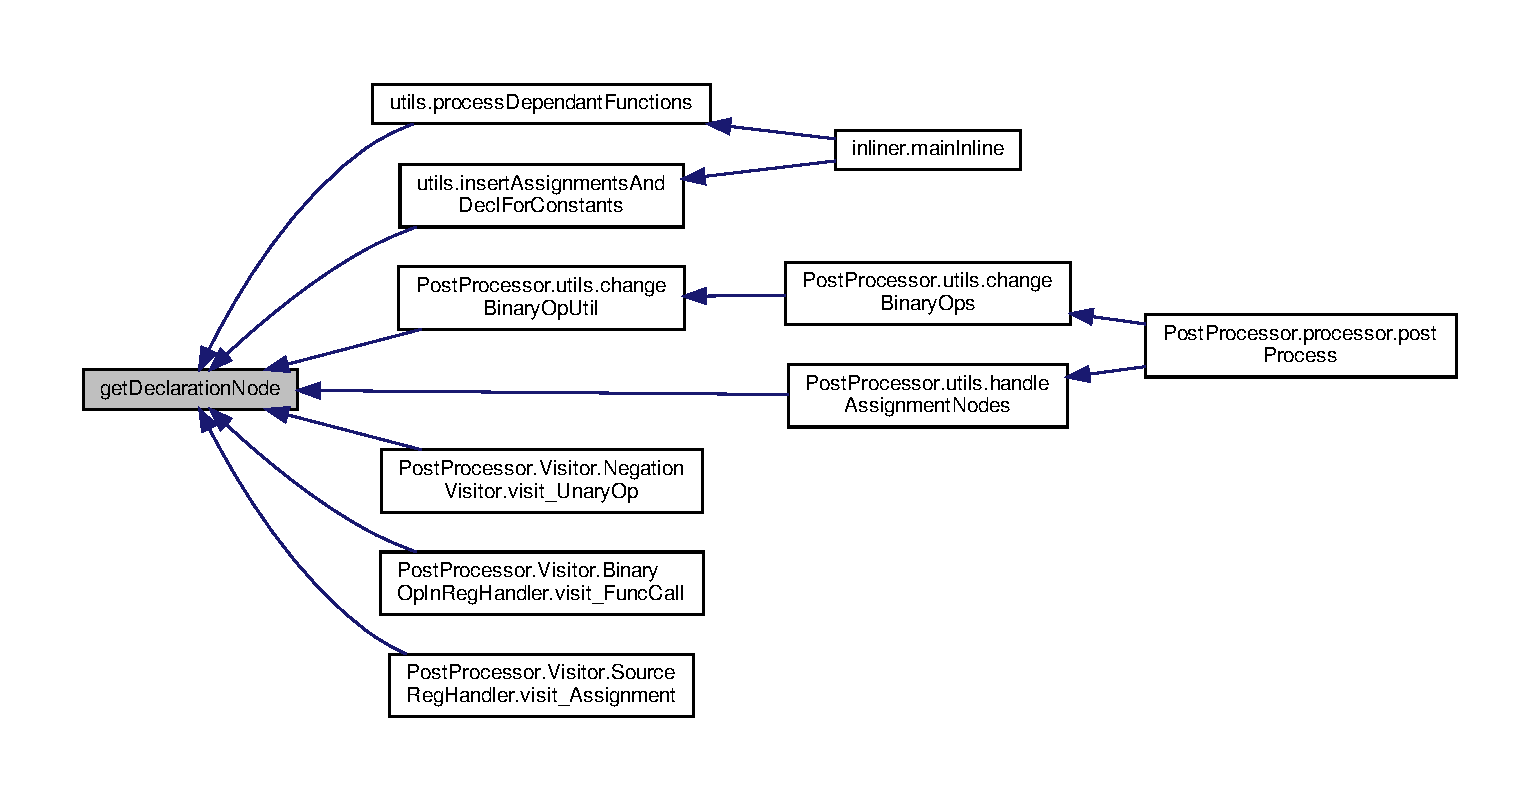
\includegraphics[width=350pt]{namespaceastNodes_ae5e5c7f09a1586002b20db6d72f6d30b_icgraph}
\end{center}
\end{figure}
\mbox{\Hypertarget{namespaceastNodes_a2403f5d006e54f20e614226280cb6cbc}\label{namespaceastNodes_a2403f5d006e54f20e614226280cb6cbc}} 
\index{ast\+Nodes@{ast\+Nodes}!get\+Simple\+Assignment\+Node@{get\+Simple\+Assignment\+Node}}
\index{get\+Simple\+Assignment\+Node@{get\+Simple\+Assignment\+Node}!ast\+Nodes@{ast\+Nodes}}
\subsubsection{\texorpdfstring{get\+Simple\+Assignment\+Node()}{getSimpleAssignmentNode()}}
{\footnotesize\ttfamily def ast\+Nodes.\+get\+Simple\+Assignment\+Node (\begin{DoxyParamCaption}\item[{}]{lvalue,  }\item[{}]{rvalue }\end{DoxyParamCaption})}

\begin{DoxyVerb}Creates a simple assignment node with the specified left-hand side and right-hand side.

@param lvalue: The left-hand side of the assignment, typically a variable name.
@type lvalue: str
@param rvalue: The right-hand side of the assignment, typically a variable name or expression.
@type rvalue: str

@return: A `c_ast.Assignment` node representing the assignment operation.
@rtype: c_ast.Assignment
\end{DoxyVerb}
 

Definition at line 7 of file ast\+Nodes.\+py.


\begin{DoxyCode}
7 \textcolor{keyword}{def }\hyperlink{namespacePostProcessor_1_1astNodes_a1fc39a0ad420aefababe0a8ee2907f4e}{getSimpleAssignmentNode}(lvalue,rvalue):
8     \textcolor{stringliteral}{"""
}
9 \textcolor{stringliteral}{    Creates a simple assignment node with the specified left-hand side and right-hand side.
}
10 \textcolor{stringliteral}{
}
11 \textcolor{stringliteral}{    @param lvalue: The left-hand side of the assignment, typically a variable name.
}
12 \textcolor{stringliteral}{    @type lvalue: str
}
13 \textcolor{stringliteral}{    @param rvalue: The right-hand side of the assignment, typically a variable name or expression.
}
14 \textcolor{stringliteral}{    @type rvalue: str
}
15 \textcolor{stringliteral}{
}
16 \textcolor{stringliteral}{    @return: A `c\_ast.Assignment` node representing the assignment operation.
}
17 \textcolor{stringliteral}{    @rtype: c\_ast.Assignment
}
18 \textcolor{stringliteral}{    """}
19     \textcolor{keywordflow}{return} c\_ast.Assignment(lvalue=c\_ast.ID(name=lvalue),rvalue=c\_ast.ID(name=rvalue),op=\textcolor{stringliteral}{'='})
20 
\end{DoxyCode}
Here is the caller graph for this function\+:\nopagebreak
\begin{figure}[H]
\begin{center}
\leavevmode
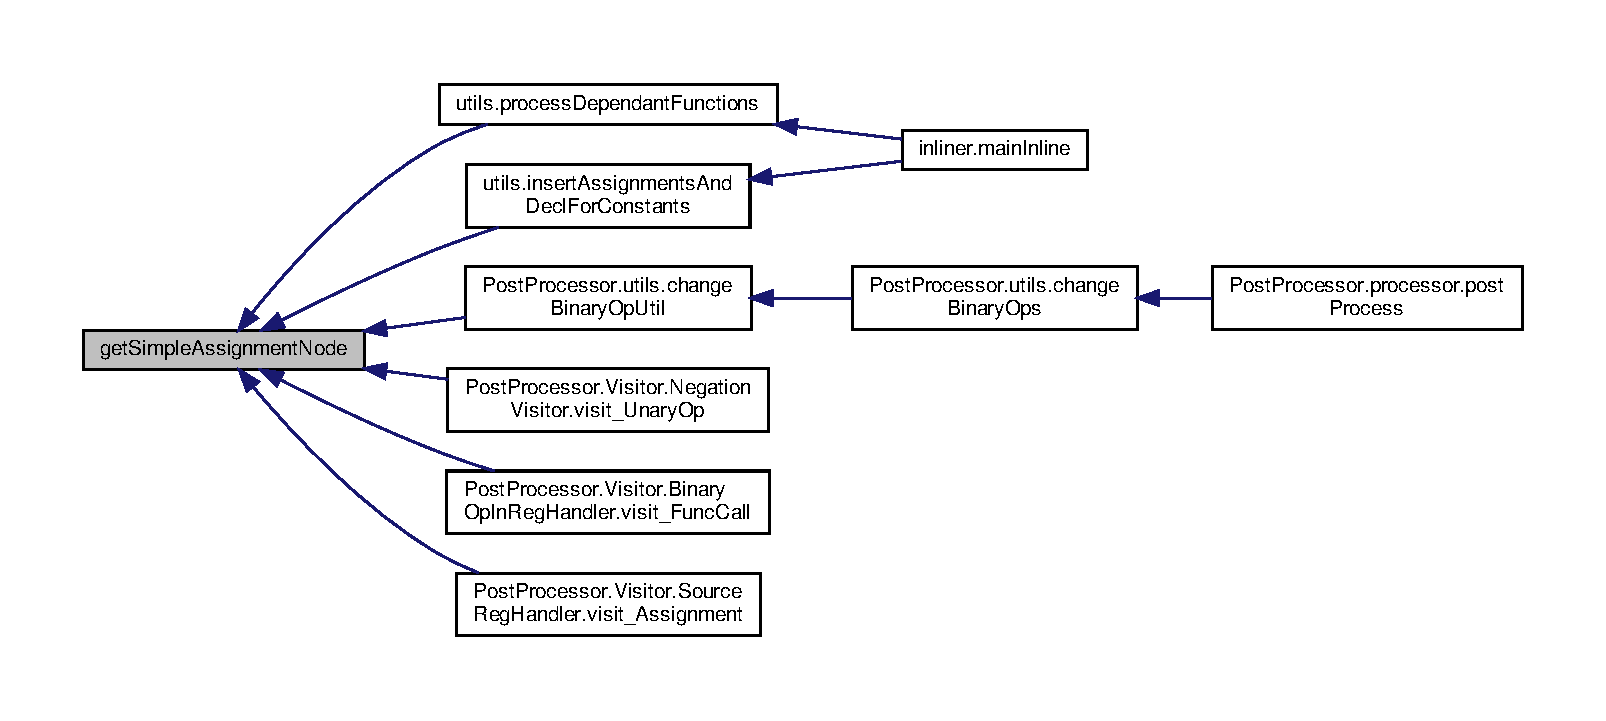
\includegraphics[width=350pt]{namespaceastNodes_a2403f5d006e54f20e614226280cb6cbc_icgraph}
\end{center}
\end{figure}

\hypertarget{namespaceblockHandlers}{}\section{block\+Handlers Namespace Reference}
\label{namespaceblockHandlers}\index{block\+Handlers@{block\+Handlers}}
\subsection*{Functions}
\begin{DoxyCompactItemize}
\item 
def \hyperlink{namespaceblockHandlers_ac54cbd08eb8b12eed0c801fa775911dd}{handle\+Assignment\+Block} (node, internal\+Variables)
\item 
def \hyperlink{namespaceblockHandlers_ad92852be9f2eee24eb76b2dd747e7584}{handle\+Decl\+Block} (node, internal\+Variables)
\item 
def \hyperlink{namespaceblockHandlers_ac034bd474478ead202ae756242b4348c}{handle\+Func\+Call\+Block} (node, functions, f\+Name, function\+Calls, internal\+Variables)
\item 
def \hyperlink{namespaceblockHandlers_a9a619208834c3d0aa0861354376f5208}{handle\+Return\+Block} (node, internal\+Variables, functions, f\+Name)
\item 
def \hyperlink{namespaceblockHandlers_a5dcb5985c58176982a44686f616daa7f}{reconstruct\+\_\+expression} (node, internal\+Variables)
\end{DoxyCompactItemize}


\subsection{Function Documentation}
\mbox{\Hypertarget{namespaceblockHandlers_ac54cbd08eb8b12eed0c801fa775911dd}\label{namespaceblockHandlers_ac54cbd08eb8b12eed0c801fa775911dd}} 
\index{block\+Handlers@{block\+Handlers}!handle\+Assignment\+Block@{handle\+Assignment\+Block}}
\index{handle\+Assignment\+Block@{handle\+Assignment\+Block}!block\+Handlers@{block\+Handlers}}
\subsubsection{\texorpdfstring{handle\+Assignment\+Block()}{handleAssignmentBlock()}}
{\footnotesize\ttfamily def block\+Handlers.\+handle\+Assignment\+Block (\begin{DoxyParamCaption}\item[{}]{node,  }\item[{}]{internal\+Variables }\end{DoxyParamCaption})}

\begin{DoxyVerb}@brief Handles assignment blocks in the AST and updates internal variables.

This function processes assignment nodes to determine the type of the variable (either "reg" or "wire") and reconstructs its assigned value.

@param node: The assignment node being processed.
@type node: pycparser.c_ast.Assignment
@param internalVariables: A dictionary to store and manage internal variables.
@type internalVariables: dict
@return: Boolean indicating if a register variable is present.
@rtype: bool
\end{DoxyVerb}
 

Definition at line 70 of file block\+Handlers.\+py.


\begin{DoxyCode}
70 \textcolor{keyword}{def }\hyperlink{namespaceblockHandlers_ac54cbd08eb8b12eed0c801fa775911dd}{handleAssignmentBlock}(node,internalVariables):
71     \textcolor{stringliteral}{"""
}
72 \textcolor{stringliteral}{    @brief Handles assignment blocks in the AST and updates internal variables.
}
73 \textcolor{stringliteral}{
}
74 \textcolor{stringliteral}{    This function processes assignment nodes to determine the type of the variable (either "reg" or "wire")
       and reconstructs its assigned value.
}
75 \textcolor{stringliteral}{
}
76 \textcolor{stringliteral}{    @param node: The assignment node being processed.
}
77 \textcolor{stringliteral}{    @type node: pycparser.c\_ast.Assignment
}
78 \textcolor{stringliteral}{    @param internalVariables: A dictionary to store and manage internal variables.
}
79 \textcolor{stringliteral}{    @type internalVariables: dict
}
80 \textcolor{stringliteral}{    @return: Boolean indicating if a register variable is present.
}
81 \textcolor{stringliteral}{    @rtype: bool
}
82 \textcolor{stringliteral}{    """}
83     regPresent = \textcolor{keyword}{False}
84     lval = node.lvalue.name \textcolor{keywordflow}{if} isinstance(node.lvalue,c\_ast.ID) \textcolor{keywordflow}{else} node.lvalue.expr.name
85     
86     \textcolor{keywordflow}{if} isinstance(node.rvalue,c\_ast.FuncCall) \textcolor{keywordflow}{and} node.rvalue.name.name == \textcolor{stringliteral}{"reg"}:
87         exp = \hyperlink{namespaceblockHandlers_a5dcb5985c58176982a44686f616daa7f}{reconstruct\_expression}(node.rvalue.args.exprs[0],internalVariables)
88         internalVariables[lval] = \{\}
89         internalVariables[lval][\textcolor{stringliteral}{"type"}] = \textcolor{stringliteral}{"reg"}
90         regPresent = \textcolor{keyword}{True}
91     \textcolor{keywordflow}{else}:
92         exp = \hyperlink{namespaceblockHandlers_a5dcb5985c58176982a44686f616daa7f}{reconstruct\_expression}(node.rvalue,internalVariables)
93         internalVariables[lval] = \{\}
94         \textcolor{keywordflow}{if} isinstance(node.lvalue,c\_ast.UnaryOp):
95             internalVariables[lval][\textcolor{stringliteral}{"type"}] = \textcolor{stringliteral}{"reg"}
96             regPresent = \textcolor{keyword}{True}
97         \textcolor{keywordflow}{else}:
98             internalVariables[lval][\textcolor{stringliteral}{"type"}] = \textcolor{stringliteral}{"wire"}
99         
100     internalVariables[lval][\textcolor{stringliteral}{"value"}] = exp
101     \textcolor{keywordflow}{return} regPresent
102 
\end{DoxyCode}
Here is the call graph for this function\+:\nopagebreak
\begin{figure}[H]
\begin{center}
\leavevmode
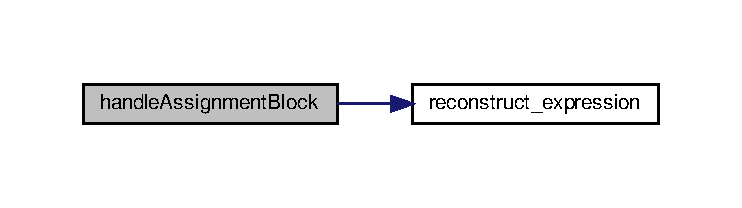
\includegraphics[width=350pt]{namespaceblockHandlers_ac54cbd08eb8b12eed0c801fa775911dd_cgraph}
\end{center}
\end{figure}
Here is the caller graph for this function\+:\nopagebreak
\begin{figure}[H]
\begin{center}
\leavevmode
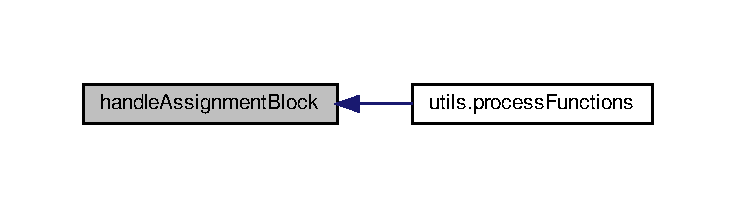
\includegraphics[width=350pt]{namespaceblockHandlers_ac54cbd08eb8b12eed0c801fa775911dd_icgraph}
\end{center}
\end{figure}
\mbox{\Hypertarget{namespaceblockHandlers_ad92852be9f2eee24eb76b2dd747e7584}\label{namespaceblockHandlers_ad92852be9f2eee24eb76b2dd747e7584}} 
\index{block\+Handlers@{block\+Handlers}!handle\+Decl\+Block@{handle\+Decl\+Block}}
\index{handle\+Decl\+Block@{handle\+Decl\+Block}!block\+Handlers@{block\+Handlers}}
\subsubsection{\texorpdfstring{handle\+Decl\+Block()}{handleDeclBlock()}}
{\footnotesize\ttfamily def block\+Handlers.\+handle\+Decl\+Block (\begin{DoxyParamCaption}\item[{}]{node,  }\item[{}]{internal\+Variables }\end{DoxyParamCaption})}

\begin{DoxyVerb}@brief Handles declaration blocks in the AST and updates internal variables.

This function processes declaration nodes to determine the type of the variable (either "reg" or "wire") and reconstructs its initial value.

@param node: The declaration node being processed.
@type node: pycparser.c_ast.Decl
@param internalVariables: A dictionary to store and manage internal variables.
@type internalVariables: dict
@return: Boolean indicating if a register variable is present.
@rtype: bool
\end{DoxyVerb}
 

Definition at line 41 of file block\+Handlers.\+py.


\begin{DoxyCode}
41 \textcolor{keyword}{def }\hyperlink{namespaceblockHandlers_ad92852be9f2eee24eb76b2dd747e7584}{handleDeclBlock}(node,internalVariables):
42     \textcolor{stringliteral}{"""
}
43 \textcolor{stringliteral}{    @brief Handles declaration blocks in the AST and updates internal variables.
}
44 \textcolor{stringliteral}{
}
45 \textcolor{stringliteral}{    This function processes declaration nodes to determine the type of the variable (either "reg" or "wire"
      ) and reconstructs its initial value.
}
46 \textcolor{stringliteral}{
}
47 \textcolor{stringliteral}{    @param node: The declaration node being processed.
}
48 \textcolor{stringliteral}{    @type node: pycparser.c\_ast.Decl
}
49 \textcolor{stringliteral}{    @param internalVariables: A dictionary to store and manage internal variables.
}
50 \textcolor{stringliteral}{    @type internalVariables: dict
}
51 \textcolor{stringliteral}{    @return: Boolean indicating if a register variable is present.
}
52 \textcolor{stringliteral}{    @rtype: bool
}
53 \textcolor{stringliteral}{    """}
54     regPresent = \textcolor{keyword}{False}
55     \textcolor{keywordflow}{if} node.name \textcolor{keywordflow}{not} \textcolor{keywordflow}{in} internalVariables:
56         internalVariables[node.name] = \{
57             \textcolor{stringliteral}{"type"} : \textcolor{stringliteral}{""},
58             \textcolor{stringliteral}{"value"} : \textcolor{stringliteral}{""}
59         \}
60     \textcolor{keywordflow}{if} isinstance(node.init,c\_ast.FuncCall) \textcolor{keywordflow}{and} node.init.name.name == \textcolor{stringliteral}{"reg"}:
61         internalVariables[node.name][\textcolor{stringliteral}{"type"}] = \textcolor{stringliteral}{"reg"}
62         regPresent = \textcolor{keyword}{True}
63         exp = \hyperlink{namespaceblockHandlers_a5dcb5985c58176982a44686f616daa7f}{reconstruct\_expression}(node.init.args.exprs[0],internalVariables)
64     \textcolor{keywordflow}{else}:
65         internalVariables[node.name][\textcolor{stringliteral}{"type"}] = \textcolor{stringliteral}{"wire"}
66         exp = \hyperlink{namespaceblockHandlers_a5dcb5985c58176982a44686f616daa7f}{reconstruct\_expression}(node.init,internalVariables)
67     internalVariables[node.name][\textcolor{stringliteral}{"value"}] = exp
68     \textcolor{keywordflow}{return} regPresent
69 
\end{DoxyCode}
Here is the call graph for this function\+:\nopagebreak
\begin{figure}[H]
\begin{center}
\leavevmode
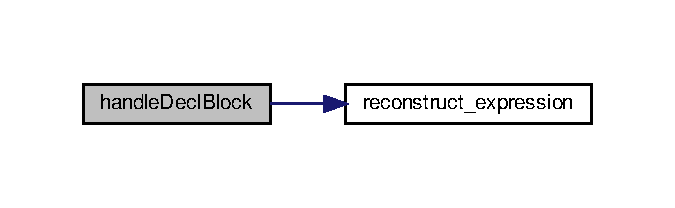
\includegraphics[width=324pt]{namespaceblockHandlers_ad92852be9f2eee24eb76b2dd747e7584_cgraph}
\end{center}
\end{figure}
Here is the caller graph for this function\+:\nopagebreak
\begin{figure}[H]
\begin{center}
\leavevmode
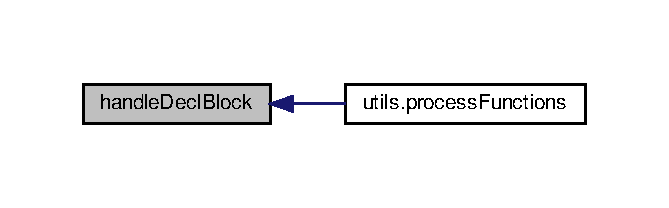
\includegraphics[width=321pt]{namespaceblockHandlers_ad92852be9f2eee24eb76b2dd747e7584_icgraph}
\end{center}
\end{figure}
\mbox{\Hypertarget{namespaceblockHandlers_ac034bd474478ead202ae756242b4348c}\label{namespaceblockHandlers_ac034bd474478ead202ae756242b4348c}} 
\index{block\+Handlers@{block\+Handlers}!handle\+Func\+Call\+Block@{handle\+Func\+Call\+Block}}
\index{handle\+Func\+Call\+Block@{handle\+Func\+Call\+Block}!block\+Handlers@{block\+Handlers}}
\subsubsection{\texorpdfstring{handle\+Func\+Call\+Block()}{handleFuncCallBlock()}}
{\footnotesize\ttfamily def block\+Handlers.\+handle\+Func\+Call\+Block (\begin{DoxyParamCaption}\item[{}]{node,  }\item[{}]{functions,  }\item[{}]{f\+Name,  }\item[{}]{function\+Calls,  }\item[{}]{internal\+Variables }\end{DoxyParamCaption})}

\begin{DoxyVerb}@brief Handles function call blocks in the AST and updates the function calls list.

This function processes function call nodes to record the function instance, parameter list, and update the function call information.

@param node: The function call node being processed.
@type node: pycparser.c_ast.FuncCall
@param functions: A dictionary containing function information.
@type functions: dict
@param fName: The name of the function making the call.
@type fName: str
@param functionCalls: A dictionary to store function calls information.
@type functionCalls: dict
@param internalVariables: A dictionary to store and manage internal variables.
@type internalVariables: dict
\end{DoxyVerb}
 

Definition at line 126 of file block\+Handlers.\+py.


\begin{DoxyCode}
126 \textcolor{keyword}{def }\hyperlink{namespaceblockHandlers_ac034bd474478ead202ae756242b4348c}{handleFuncCallBlock}(node,functions,fName,functionCalls,internalVariables):
127     \textcolor{stringliteral}{"""
}
128 \textcolor{stringliteral}{    @brief Handles function call blocks in the AST and updates the function calls list.
}
129 \textcolor{stringliteral}{
}
130 \textcolor{stringliteral}{    This function processes function call nodes to record the function instance, parameter list, and update
       the function call information.
}
131 \textcolor{stringliteral}{
}
132 \textcolor{stringliteral}{    @param node: The function call node being processed.
}
133 \textcolor{stringliteral}{    @type node: pycparser.c\_ast.FuncCall
}
134 \textcolor{stringliteral}{    @param functions: A dictionary containing function information.
}
135 \textcolor{stringliteral}{    @type functions: dict
}
136 \textcolor{stringliteral}{    @param fName: The name of the function making the call.
}
137 \textcolor{stringliteral}{    @type fName: str
}
138 \textcolor{stringliteral}{    @param functionCalls: A dictionary to store function calls information.
}
139 \textcolor{stringliteral}{    @type functionCalls: dict
}
140 \textcolor{stringliteral}{    @param internalVariables: A dictionary to store and manage internal variables.
}
141 \textcolor{stringliteral}{    @type internalVariables: dict
}
142 \textcolor{stringliteral}{    """}
143     called = functions[fName][\textcolor{stringliteral}{"called"}];
144     called = called + 1
145     inst = node.name.name + str(called)
146     functions[fName][\textcolor{stringliteral}{"called"}] = called
147     paramList = []
148     paramList.append(\textcolor{stringliteral}{"clk"})
149     \textcolor{keywordflow}{for} expr \textcolor{keywordflow}{in} node.args.exprs:
150         \textcolor{keywordflow}{if} isinstance(expr,c\_ast.UnaryOp):
151             exp = \hyperlink{namespaceblockHandlers_a5dcb5985c58176982a44686f616daa7f}{reconstruct\_expression}(expr.expr,internalVariables)
152         \textcolor{keywordflow}{else}:
153             exp = \hyperlink{namespaceblockHandlers_a5dcb5985c58176982a44686f616daa7f}{reconstruct\_expression}(expr,internalVariables)
154         paramList.append(exp)
155     functionCalls[fName].append(\{
156         \textcolor{stringliteral}{"instanceName"} : inst,
157         \textcolor{stringliteral}{"paramList"} : paramList,
158         \textcolor{stringliteral}{"callee"} : node.name.name
159     \}
\end{DoxyCode}
Here is the call graph for this function\+:\nopagebreak
\begin{figure}[H]
\begin{center}
\leavevmode
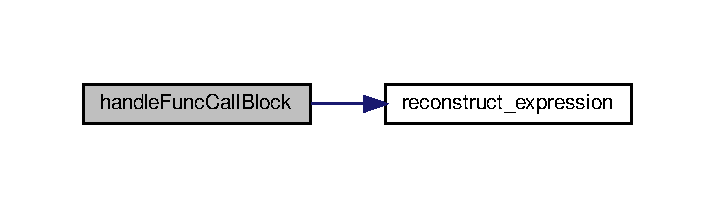
\includegraphics[width=343pt]{namespaceblockHandlers_ac034bd474478ead202ae756242b4348c_cgraph}
\end{center}
\end{figure}
Here is the caller graph for this function\+:\nopagebreak
\begin{figure}[H]
\begin{center}
\leavevmode
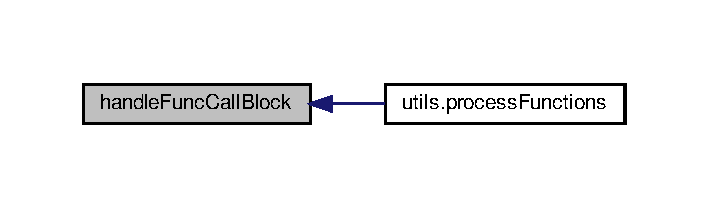
\includegraphics[width=340pt]{namespaceblockHandlers_ac034bd474478ead202ae756242b4348c_icgraph}
\end{center}
\end{figure}
\mbox{\Hypertarget{namespaceblockHandlers_a9a619208834c3d0aa0861354376f5208}\label{namespaceblockHandlers_a9a619208834c3d0aa0861354376f5208}} 
\index{block\+Handlers@{block\+Handlers}!handle\+Return\+Block@{handle\+Return\+Block}}
\index{handle\+Return\+Block@{handle\+Return\+Block}!block\+Handlers@{block\+Handlers}}
\subsubsection{\texorpdfstring{handle\+Return\+Block()}{handleReturnBlock()}}
{\footnotesize\ttfamily def block\+Handlers.\+handle\+Return\+Block (\begin{DoxyParamCaption}\item[{}]{node,  }\item[{}]{internal\+Variables,  }\item[{}]{functions,  }\item[{}]{f\+Name }\end{DoxyParamCaption})}

\begin{DoxyVerb}@brief Handles return blocks in the AST and updates function outputs.

This function processes return nodes to identify output variables and updates the function's output list or internal variables accordingly.

@param node: The return node being processed.
@type node: pycparser.c_ast.Return
@param internalVariables: A dictionary to store and manage internal variables.
@type internalVariables: dict
@param functions: A dictionary containing function information.
@type functions: dict
@param fName: The name of the function being processed.
@type fName: str
\end{DoxyVerb}
 

Definition at line 103 of file block\+Handlers.\+py.


\begin{DoxyCode}
103 \textcolor{keyword}{def }\hyperlink{namespaceblockHandlers_a9a619208834c3d0aa0861354376f5208}{handleReturnBlock}(node,internalVariables,functions,fName):
104     \textcolor{stringliteral}{"""
}
105 \textcolor{stringliteral}{    @brief Handles return blocks in the AST and updates function outputs.
}
106 \textcolor{stringliteral}{
}
107 \textcolor{stringliteral}{    This function processes return nodes to identify output variables and updates the function's output
       list or internal variables accordingly.
}
108 \textcolor{stringliteral}{
}
109 \textcolor{stringliteral}{    @param node: The return node being processed.
}
110 \textcolor{stringliteral}{    @type node: pycparser.c\_ast.Return
}
111 \textcolor{stringliteral}{    @param internalVariables: A dictionary to store and manage internal variables.
}
112 \textcolor{stringliteral}{    @type internalVariables: dict
}
113 \textcolor{stringliteral}{    @param functions: A dictionary containing function information.
}
114 \textcolor{stringliteral}{    @type functions: dict
}
115 \textcolor{stringliteral}{    @param fName: The name of the function being processed.
}
116 \textcolor{stringliteral}{    @type fName: str
}
117 \textcolor{stringliteral}{    """}
118     \textcolor{keywordflow}{if} isinstance(node.expr,c\_ast.ID):
119         \textcolor{keywordflow}{if} node.expr.name \textcolor{keywordflow}{not} \textcolor{keywordflow}{in} functions[fName][\textcolor{stringliteral}{"outputs"}]:
120             functions[fName][\textcolor{stringliteral}{"outputs"}].append(node.expr.name)
121     \textcolor{keywordflow}{elif} isinstance(node.expr, c\_ast.BinaryOp):
122         internalVariables[\textcolor{stringliteral}{"r\_val"}] = \{\}
123         internalVariables[\textcolor{stringliteral}{"r\_val"}][\textcolor{stringliteral}{"type"}] = \textcolor{stringliteral}{"wire"}
124         internalVariables[\textcolor{stringliteral}{"r\_val"}][\textcolor{stringliteral}{"value"}] = \hyperlink{namespaceblockHandlers_a5dcb5985c58176982a44686f616daa7f}{reconstruct\_expression}(node.expr,
      internalVariables)
125 
\end{DoxyCode}
Here is the call graph for this function\+:\nopagebreak
\begin{figure}[H]
\begin{center}
\leavevmode
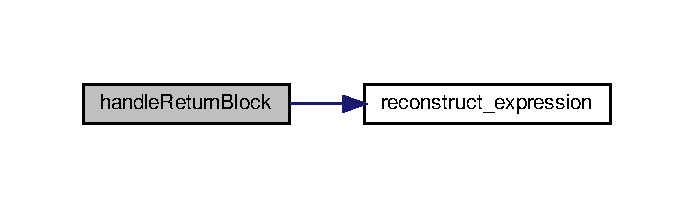
\includegraphics[width=333pt]{namespaceblockHandlers_a9a619208834c3d0aa0861354376f5208_cgraph}
\end{center}
\end{figure}
Here is the caller graph for this function\+:\nopagebreak
\begin{figure}[H]
\begin{center}
\leavevmode
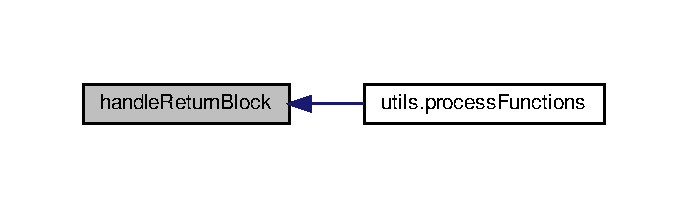
\includegraphics[width=330pt]{namespaceblockHandlers_a9a619208834c3d0aa0861354376f5208_icgraph}
\end{center}
\end{figure}
\mbox{\Hypertarget{namespaceblockHandlers_a5dcb5985c58176982a44686f616daa7f}\label{namespaceblockHandlers_a5dcb5985c58176982a44686f616daa7f}} 
\index{block\+Handlers@{block\+Handlers}!reconstruct\+\_\+expression@{reconstruct\+\_\+expression}}
\index{reconstruct\+\_\+expression@{reconstruct\+\_\+expression}!block\+Handlers@{block\+Handlers}}
\subsubsection{\texorpdfstring{reconstruct\+\_\+expression()}{reconstruct\_expression()}}
{\footnotesize\ttfamily def block\+Handlers.\+reconstruct\+\_\+expression (\begin{DoxyParamCaption}\item[{}]{node,  }\item[{}]{internal\+Variables }\end{DoxyParamCaption})}

\begin{DoxyVerb}@brief Recursively reconstructs expressions from AST nodes.

This function converts AST nodes into a string representation of the expression they represent. It supports binary operations, unary operations, constants, identifiers, and function calls.

@param node: The AST node representing an expression.
@type node: pycparser.c_ast.Node
@param internalVariables: A dictionary to store and manage internal variables.
@type internalVariables: dict
@return: A string representing the reconstructed expression.
@rtype: str
@raises ValueError: If the node type is unsupported.
\end{DoxyVerb}
 

Definition at line 4 of file block\+Handlers.\+py.


\begin{DoxyCode}
4 \textcolor{keyword}{def }\hyperlink{namespaceblockHandlers_a5dcb5985c58176982a44686f616daa7f}{reconstruct\_expression}(node,internalVariables):
5     \textcolor{stringliteral}{"""
}
6 \textcolor{stringliteral}{    @brief Recursively reconstructs expressions from AST nodes.
}
7 \textcolor{stringliteral}{
}
8 \textcolor{stringliteral}{    This function converts AST nodes into a string representation of the expression they represent. It
       supports binary operations, unary operations, constants, identifiers, and function calls.
}
9 \textcolor{stringliteral}{
}
10 \textcolor{stringliteral}{    @param node: The AST node representing an expression.
}
11 \textcolor{stringliteral}{    @type node: pycparser.c\_ast.Node
}
12 \textcolor{stringliteral}{    @param internalVariables: A dictionary to store and manage internal variables.
}
13 \textcolor{stringliteral}{    @type internalVariables: dict
}
14 \textcolor{stringliteral}{    @return: A string representing the reconstructed expression.
}
15 \textcolor{stringliteral}{    @rtype: str
}
16 \textcolor{stringliteral}{    @raises ValueError: If the node type is unsupported.
}
17 \textcolor{stringliteral}{    """}
18     \textcolor{keywordflow}{if} isinstance(node, c\_ast.BinaryOp):
19         leftExpr = \hyperlink{namespaceblockHandlers_a5dcb5985c58176982a44686f616daa7f}{reconstruct\_expression}(node.left,internalVariables)
20         rightExpr = \hyperlink{namespaceblockHandlers_a5dcb5985c58176982a44686f616daa7f}{reconstruct\_expression}(node.right,internalVariables)
21         \textcolor{keywordflow}{return} f\textcolor{stringliteral}{"(\{leftExpr\} \{node.op\} \{rightExpr\})"}
22     \textcolor{keywordflow}{elif} isinstance(node, c\_ast.ID):
23         \textcolor{keywordflow}{return} node.name
24     \textcolor{keywordflow}{elif} isinstance(node,c\_ast.Constant):
25         \textcolor{keywordflow}{return} node.value
26     \textcolor{keywordflow}{elif} isinstance(node,c\_ast.UnaryOp):
27         \textcolor{keywordflow}{return} \textcolor{stringliteral}{"!"} + \hyperlink{namespaceblockHandlers_a5dcb5985c58176982a44686f616daa7f}{reconstruct\_expression}(node.expr,internalVariables)
28     \textcolor{keywordflow}{elif} isinstance(node,c\_ast.FuncCall):
29         \textcolor{keywordflow}{if} node.name.name == \textcolor{stringliteral}{"reg"}:
30             varName = str(node.args.exprs[0].name) + \textcolor{stringliteral}{"\_reg"};
31             \textcolor{keywordflow}{if} varName \textcolor{keywordflow}{not} \textcolor{keywordflow}{in} internalVariables:
32                 internalVariables[varName] = \{
33                     \textcolor{stringliteral}{"type"} : \textcolor{stringliteral}{"reg"},
34                     \textcolor{stringliteral}{"value"} : str(node.args.exprs[0].name)
35                 \}
36             \textcolor{keywordflow}{return} varName;
37     \textcolor{keywordflow}{else}:
38         \textcolor{keywordflow}{raise} ValueError(f\textcolor{stringliteral}{"Unsupported node type: \{type(node).\_\_name\_\_\}"})
39 
40 \textcolor{comment}{#block handlers for corresponding blocks/nodes
}
\end{DoxyCode}
Here is the caller graph for this function\+:\nopagebreak
\begin{figure}[H]
\begin{center}
\leavevmode
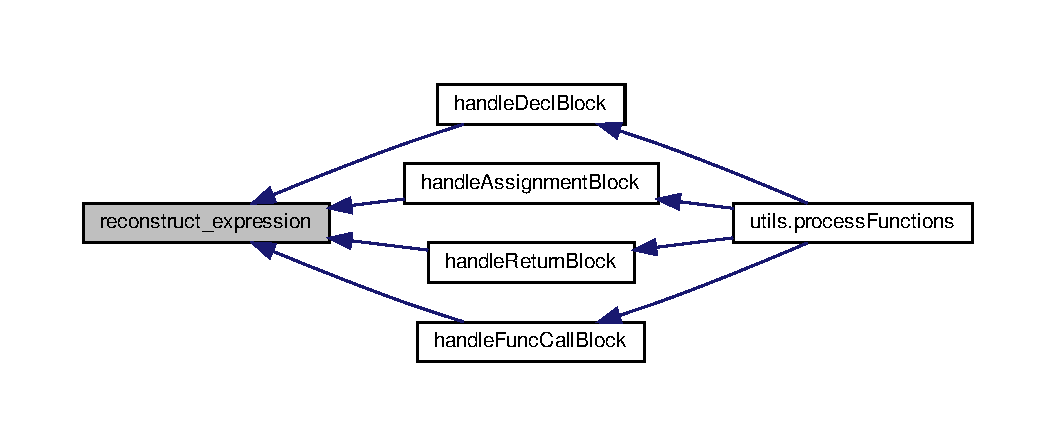
\includegraphics[width=350pt]{namespaceblockHandlers_a5dcb5985c58176982a44686f616daa7f_icgraph}
\end{center}
\end{figure}

\hypertarget{namespaceDiGraph}{}\section{Di\+Graph Namespace Reference}
\label{namespaceDiGraph}\index{Di\+Graph@{Di\+Graph}}
\subsection*{Classes}
\begin{DoxyCompactItemize}
\item 
class \hyperlink{classDiGraph_1_1DiGraph}{Di\+Graph}
\end{DoxyCompactItemize}

\hypertarget{namespaceinliner}{}\section{inliner Namespace Reference}
\label{namespaceinliner}\index{inliner@{inliner}}
\subsection*{Functions}
\begin{DoxyCompactItemize}
\item 
def \hyperlink{namespaceinliner_a85ff5417ce309a641abfa41d26e8d7f3}{main\+Inline} (input\+File, output\+File, top\+Module)
\end{DoxyCompactItemize}
\subsection*{Variables}
\begin{DoxyCompactItemize}
\item 
\hyperlink{namespaceinliner_a8187411843a6284ffb964ef3fb9fcab3}{args} = json.\+load(file)
\end{DoxyCompactItemize}


\subsection{Function Documentation}
\mbox{\Hypertarget{namespaceinliner_a85ff5417ce309a641abfa41d26e8d7f3}\label{namespaceinliner_a85ff5417ce309a641abfa41d26e8d7f3}} 
\index{inliner@{inliner}!main\+Inline@{main\+Inline}}
\index{main\+Inline@{main\+Inline}!inliner@{inliner}}
\subsubsection{\texorpdfstring{main\+Inline()}{mainInline()}}
{\footnotesize\ttfamily def inliner.\+main\+Inline (\begin{DoxyParamCaption}\item[{}]{input\+File,  }\item[{}]{output\+File,  }\item[{}]{top\+Module }\end{DoxyParamCaption})}

\begin{DoxyVerb}@brief Processes a C source file to inline functions, handle constants, and generate a new C file.

This function parses the provided C source file, constructs a directed graph of functions, performs topological
sorting, processes functions based on dependencies, handles array and constant values, and finally generates
an updated C source file.

@param inputFile: The path to the input C source file to be processed.
@type inputFile: str
@param outputFile: The path where the processed C source file will be saved.
@type outputFile: str
@param topModule: The name of the top-level module (function) to be used as the entry point.
@type topModule: str

@raises SystemExit: If the top module is not found in the sorted function list or if no functions are present.
\end{DoxyVerb}
 

Definition at line 12 of file inliner.\+py.


\begin{DoxyCode}
12 \textcolor{keyword}{def }\hyperlink{namespaceinliner_a85ff5417ce309a641abfa41d26e8d7f3}{mainInline}(inputFile,outputFile,topModule):
13     \textcolor{stringliteral}{"""
}
14 \textcolor{stringliteral}{    @brief Processes a C source file to inline functions, handle constants, and generate a new C file.
}
15 \textcolor{stringliteral}{
}
16 \textcolor{stringliteral}{    This function parses the provided C source file, constructs a directed graph of functions, performs
       topological
}
17 \textcolor{stringliteral}{    sorting, processes functions based on dependencies, handles array and constant values, and finally
       generates
}
18 \textcolor{stringliteral}{    an updated C source file.
}
19 \textcolor{stringliteral}{
}
20 \textcolor{stringliteral}{    @param inputFile: The path to the input C source file to be processed.
}
21 \textcolor{stringliteral}{    @type inputFile: str
}
22 \textcolor{stringliteral}{    @param outputFile: The path where the processed C source file will be saved.
}
23 \textcolor{stringliteral}{    @type outputFile: str
}
24 \textcolor{stringliteral}{    @param topModule: The name of the top-level module (function) to be used as the entry point.
}
25 \textcolor{stringliteral}{    @type topModule: str
}
26 \textcolor{stringliteral}{
}
27 \textcolor{stringliteral}{    @raises SystemExit: If the top module is not found in the sorted function list or if no functions are
       present.
}
28 \textcolor{stringliteral}{    """}
29     ast = parse\_file(inputFile, use\_cpp=\textcolor{keyword}{True})
30     arrMap = \{\}
31     arrVisitor = DeclVisitor(arrayMap=arrMap,ast=ast)
32     arrVisitor.visit(ast)
33     functionGraph = \hyperlink{namespaceDiGraph}{DiGraph}()
34     functionInfo = \{\}
35 
36     \textcolor{keywordflow}{for} fDef \textcolor{keywordflow}{in} ast.ext:
37         \textcolor{keywordflow}{if} isinstance(fDef,c\_ast.FuncDef):
38             functionGraph.addFunction(fDef.decl.name)
39             visitor = FunctionVisitor(functionGraph,fDef.decl.name)
40             visitor.visit(fDef)
41 
42     sortedList = functionGraph.topoSort()
43     \textcolor{keywordflow}{if} topModule \textcolor{keywordflow}{not} \textcolor{keywordflow}{in} sortedList:
44         print(f\textcolor{stringliteral}{"No top module named \{topModule\} in given input file."})
45         print(\textcolor{stringliteral}{"Note : The name of module is case sensitive"})
46         sys.exit(1)
47     if(len(sortedList) == 1):
48         \hyperlink{namespaceutils_a5ab527c9affdfd39949f2e88c4299989}{generate\_c\_file}(ast,outputFile)
49 
50 
51     \textcolor{keywordflow}{for} function \textcolor{keywordflow}{in} sortedList:
52         inDegree = functionGraph.getIndegreeOf(function)
53         \textcolor{keywordflow}{if} inDegree == 0:
54             \textcolor{keywordflow}{for} fDef \textcolor{keywordflow}{in} ast.ext[:]:
55                 \textcolor{keywordflow}{if} isinstance(fDef,c\_ast.FuncDef) \textcolor{keywordflow}{and} fDef.decl.name == function:
56                     \hyperlink{namespaceutils_a01c8b36149daaab35946bf42cf90fcc1}{extractFunctionInfo}(fDef,functionInfo)
57                     ast.ext.remove(fDef)
58                     \textcolor{keywordflow}{break}
59         
60         \textcolor{keywordflow}{elif} function != topModule:
61             \textcolor{keywordflow}{for} fDef \textcolor{keywordflow}{in} ast.ext[:]:
62                 \textcolor{keywordflow}{if} isinstance(fDef,c\_ast.FuncDef) \textcolor{keywordflow}{and} fDef.decl.name == function:
63                     \hyperlink{namespaceutils_a6c1d5e886507ec0741fb0fce3f642c5b}{processDependantFunctions}(fDef,functionInfo,\textcolor{keyword}{False})
64                     \hyperlink{namespaceutils_a01c8b36149daaab35946bf42cf90fcc1}{extractFunctionInfo}(fDef,functionInfo)
65                     ast.ext.remove(fDef)
66                     \textcolor{keywordflow}{break}
67         \textcolor{keywordflow}{else}:
68             \textcolor{keywordflow}{for} fDef \textcolor{keywordflow}{in} ast.ext[:]:
69                 \textcolor{keywordflow}{if} isinstance(fDef,c\_ast.FuncDef) \textcolor{keywordflow}{and} fDef.decl.name == function:
70                     \hyperlink{namespaceutils_a6c1d5e886507ec0741fb0fce3f642c5b}{processDependantFunctions}(fDef,functionInfo,\textcolor{keyword}{True})
71     
72     \textcolor{keywordflow}{for} fDef \textcolor{keywordflow}{in} ast.ext[:]:
73         \textcolor{keywordflow}{if} isinstance(fDef,c\_ast.Decl) \textcolor{keywordflow}{and} isinstance(fDef.type,c\_ast.ArrayDecl):
74             ast.ext.remove(fDef)
75 
76     constArr = []
77     arrValueReplacer = ArrayValueReplacer(arrMap,constArr)
78     arrValueReplacer.visit(ast)
79 
80     constToVar = ConstToVar()
81     constToVar.visit(ast)
82     \hyperlink{namespaceutils_a694fa47d55cc41b3f9e86ab2f90e98f3}{insertAssignmentsAndDeclForConstants}(ast,constArr)
83 
84     assignmentChecker = AssignmentChecker();
85     assignmentChecker.visit(ast)
86     \hyperlink{namespaceutils_a5ab527c9affdfd39949f2e88c4299989}{generate\_c\_file}(ast,outputFile)
87 
88 
89 
\end{DoxyCode}
Here is the call graph for this function\+:\nopagebreak
\begin{figure}[H]
\begin{center}
\leavevmode
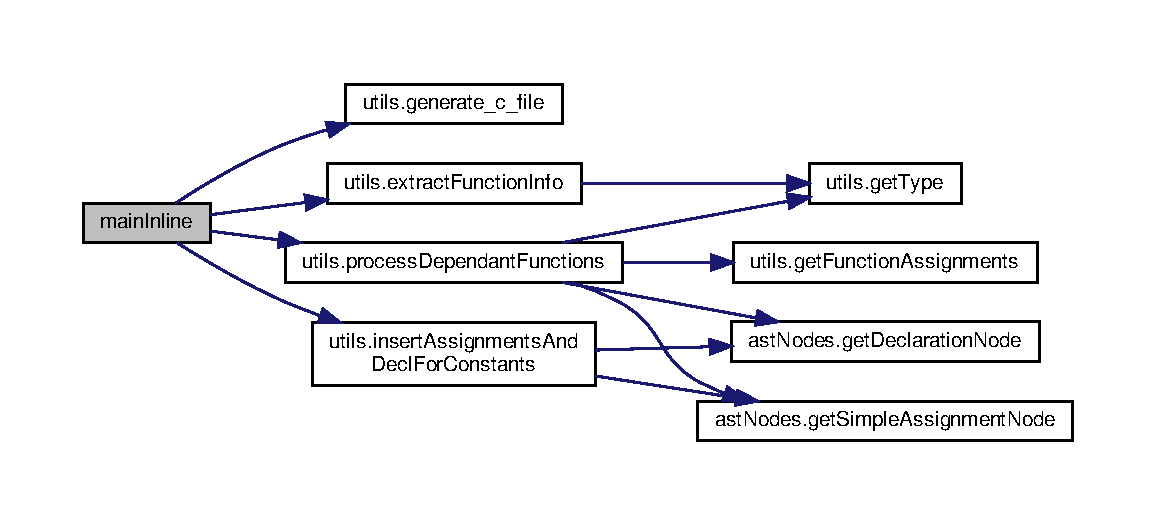
\includegraphics[width=350pt]{namespaceinliner_a85ff5417ce309a641abfa41d26e8d7f3_cgraph}
\end{center}
\end{figure}


\subsection{Variable Documentation}
\mbox{\Hypertarget{namespaceinliner_a8187411843a6284ffb964ef3fb9fcab3}\label{namespaceinliner_a8187411843a6284ffb964ef3fb9fcab3}} 
\index{inliner@{inliner}!args@{args}}
\index{args@{args}!inliner@{inliner}}
\subsubsection{\texorpdfstring{args}{args}}
{\footnotesize\ttfamily args = json.\+load(file)}



Definition at line 92 of file inliner.\+py.


\hypertarget{namespaceparser__1}{}\section{parser\+\_\+1 Namespace Reference}
\label{namespaceparser__1}\index{parser\+\_\+1@{parser\+\_\+1}}
\subsection*{Variables}
\begin{DoxyCompactItemize}
\item 
\hyperlink{namespaceparser__1_a8187411843a6284ffb964ef3fb9fcab3}{args} = json.\+load(file)
\item 
\hyperlink{namespaceparser__1_a83d838e3813fb5999c0492e0d9474bd9}{ast} = parse\+\_\+file(\hyperlink{namespaceparser__1_a8187411843a6284ffb964ef3fb9fcab3}{args}\mbox{[}\char`\"{}post\+Processor\+Output\char`\"{}\mbox{]}, use\+\_\+cpp=True)
\item 
dictionary \hyperlink{namespaceparser__1_a8915929c38e1651aaa8c716f8f8a2f0f}{function\+Calls} = \{\}
\item 
dictionary \hyperlink{namespaceparser__1_ac310aa598d85b31cc0acea80dcc3c083}{functions} = \{\}
\item 
dictionary \hyperlink{namespaceparser__1_a91478035202a21bdb18a2e8f291ab7b5}{intermediate\+Assignments} = \{\}
\item 
\hyperlink{namespaceparser__1_a5558ace5433f9aabbf0a0ec059900d94}{width} = str(\hyperlink{namespaceparser__1_a8187411843a6284ffb964ef3fb9fcab3}{args}\mbox{[}\char`\"{}bit\+Width\char`\"{}\mbox{]} -\/ 1)
\end{DoxyCompactItemize}


\subsection{Variable Documentation}
\mbox{\Hypertarget{namespaceparser__1_a8187411843a6284ffb964ef3fb9fcab3}\label{namespaceparser__1_a8187411843a6284ffb964ef3fb9fcab3}} 
\index{parser\+\_\+1@{parser\+\_\+1}!args@{args}}
\index{args@{args}!parser\+\_\+1@{parser\+\_\+1}}
\subsubsection{\texorpdfstring{args}{args}}
{\footnotesize\ttfamily args = json.\+load(file)}



Definition at line 27 of file parser\+\_\+1.\+py.

\mbox{\Hypertarget{namespaceparser__1_a83d838e3813fb5999c0492e0d9474bd9}\label{namespaceparser__1_a83d838e3813fb5999c0492e0d9474bd9}} 
\index{parser\+\_\+1@{parser\+\_\+1}!ast@{ast}}
\index{ast@{ast}!parser\+\_\+1@{parser\+\_\+1}}
\subsubsection{\texorpdfstring{ast}{ast}}
{\footnotesize\ttfamily ast = parse\+\_\+file(\hyperlink{namespaceparser__1_a8187411843a6284ffb964ef3fb9fcab3}{args}\mbox{[}\char`\"{}post\+Processor\+Output\char`\"{}\mbox{]}, use\+\_\+cpp=True)}



Definition at line 32 of file parser\+\_\+1.\+py.

\mbox{\Hypertarget{namespaceparser__1_a8915929c38e1651aaa8c716f8f8a2f0f}\label{namespaceparser__1_a8915929c38e1651aaa8c716f8f8a2f0f}} 
\index{parser\+\_\+1@{parser\+\_\+1}!function\+Calls@{function\+Calls}}
\index{function\+Calls@{function\+Calls}!parser\+\_\+1@{parser\+\_\+1}}
\subsubsection{\texorpdfstring{function\+Calls}{functionCalls}}
{\footnotesize\ttfamily dictionary function\+Calls = \{\}}



Definition at line 31 of file parser\+\_\+1.\+py.

\mbox{\Hypertarget{namespaceparser__1_ac310aa598d85b31cc0acea80dcc3c083}\label{namespaceparser__1_ac310aa598d85b31cc0acea80dcc3c083}} 
\index{parser\+\_\+1@{parser\+\_\+1}!functions@{functions}}
\index{functions@{functions}!parser\+\_\+1@{parser\+\_\+1}}
\subsubsection{\texorpdfstring{functions}{functions}}
{\footnotesize\ttfamily dictionary functions = \{\}}



Definition at line 30 of file parser\+\_\+1.\+py.

\mbox{\Hypertarget{namespaceparser__1_a91478035202a21bdb18a2e8f291ab7b5}\label{namespaceparser__1_a91478035202a21bdb18a2e8f291ab7b5}} 
\index{parser\+\_\+1@{parser\+\_\+1}!intermediate\+Assignments@{intermediate\+Assignments}}
\index{intermediate\+Assignments@{intermediate\+Assignments}!parser\+\_\+1@{parser\+\_\+1}}
\subsubsection{\texorpdfstring{intermediate\+Assignments}{intermediateAssignments}}
{\footnotesize\ttfamily dictionary intermediate\+Assignments = \{\}}



Definition at line 34 of file parser\+\_\+1.\+py.

\mbox{\Hypertarget{namespaceparser__1_a5558ace5433f9aabbf0a0ec059900d94}\label{namespaceparser__1_a5558ace5433f9aabbf0a0ec059900d94}} 
\index{parser\+\_\+1@{parser\+\_\+1}!width@{width}}
\index{width@{width}!parser\+\_\+1@{parser\+\_\+1}}
\subsubsection{\texorpdfstring{width}{width}}
{\footnotesize\ttfamily width = str(\hyperlink{namespaceparser__1_a8187411843a6284ffb964ef3fb9fcab3}{args}\mbox{[}\char`\"{}bit\+Width\char`\"{}\mbox{]} -\/ 1)}



Definition at line 29 of file parser\+\_\+1.\+py.


\hypertarget{namespacePostProcessor}{}\section{Post\+Processor Namespace Reference}
\label{namespacePostProcessor}\index{Post\+Processor@{Post\+Processor}}
\subsection*{Namespaces}
\begin{DoxyCompactItemize}
\item 
 \hyperlink{namespacePostProcessor_1_1astNodes}{ast\+Nodes}
\item 
 \hyperlink{namespacePostProcessor_1_1globalVariables}{global\+Variables}
\item 
 \hyperlink{namespacePostProcessor_1_1processor}{processor}
\item 
 \hyperlink{namespacePostProcessor_1_1utils}{utils}
\item 
 \hyperlink{namespacePostProcessor_1_1Visitor}{Visitor}
\end{DoxyCompactItemize}

\hypertarget{namespacePostProcessor_1_1astNodes}{}\section{Post\+Processor.\+ast\+Nodes Namespace Reference}
\label{namespacePostProcessor_1_1astNodes}\index{Post\+Processor.\+ast\+Nodes@{Post\+Processor.\+ast\+Nodes}}
\subsection*{Functions}
\begin{DoxyCompactItemize}
\item 
def \hyperlink{namespacePostProcessor_1_1astNodes_aa6c634c9a1dceb3e9cc65cadadf5f450}{get\+Assignment\+Node} (operands, operator, var\+To\+Assign)
\item 
def \hyperlink{namespacePostProcessor_1_1astNodes_aebd6602b5bdafed24833f298500fd85c}{get\+Declaration\+Node} (id\+Name)
\item 
def \hyperlink{namespacePostProcessor_1_1astNodes_afb1489449acb633bf78b48165fe578be}{get\+Left\+Or\+Right\+Node\+Of\+Assignment} (operand)
\item 
def \hyperlink{namespacePostProcessor_1_1astNodes_a30de65f8e1753733f88a01d42927ef1b}{get\+Reg\+Func\+Call\+Node} (name)
\item 
def \hyperlink{namespacePostProcessor_1_1astNodes_a1fc39a0ad420aefababe0a8ee2907f4e}{get\+Simple\+Assignment\+Node} (lvalue, rvalue)
\end{DoxyCompactItemize}


\subsection{Function Documentation}
\mbox{\Hypertarget{namespacePostProcessor_1_1astNodes_aa6c634c9a1dceb3e9cc65cadadf5f450}\label{namespacePostProcessor_1_1astNodes_aa6c634c9a1dceb3e9cc65cadadf5f450}} 
\index{Post\+Processor\+::ast\+Nodes@{Post\+Processor\+::ast\+Nodes}!get\+Assignment\+Node@{get\+Assignment\+Node}}
\index{get\+Assignment\+Node@{get\+Assignment\+Node}!Post\+Processor\+::ast\+Nodes@{Post\+Processor\+::ast\+Nodes}}
\subsubsection{\texorpdfstring{get\+Assignment\+Node()}{getAssignmentNode()}}
{\footnotesize\ttfamily def Post\+Processor.\+ast\+Nodes.\+get\+Assignment\+Node (\begin{DoxyParamCaption}\item[{}]{operands,  }\item[{}]{operator,  }\item[{}]{var\+To\+Assign }\end{DoxyParamCaption})}

\begin{DoxyVerb}Creates an assignment node with a binary operation if there are multiple operands, or a single operand otherwise.

@param operands: A list of operands for the assignment.
@type operands: list of str
@param operator: The operator to use if there are multiple operands.
@type operator: str
@param varToAssign: The variable name to which the result is assigned.
@type varToAssign: str

@return: A `c_ast.Assignment` node with the specified operands and operator.
@rtype: c_ast.Assignment
\end{DoxyVerb}
 

Definition at line 53 of file ast\+Nodes.\+py.


\begin{DoxyCode}
53 \textcolor{keyword}{def }\hyperlink{namespacePostProcessor_1_1astNodes_aa6c634c9a1dceb3e9cc65cadadf5f450}{getAssignmentNode}(operands,operator,varToAssign):
54     \textcolor{stringliteral}{"""
}
55 \textcolor{stringliteral}{    Creates an assignment node with a binary operation if there are multiple operands, or a single operand
       otherwise.
}
56 \textcolor{stringliteral}{
}
57 \textcolor{stringliteral}{    @param operands: A list of operands for the assignment.
}
58 \textcolor{stringliteral}{    @type operands: list of str
}
59 \textcolor{stringliteral}{    @param operator: The operator to use if there are multiple operands.
}
60 \textcolor{stringliteral}{    @type operator: str
}
61 \textcolor{stringliteral}{    @param varToAssign: The variable name to which the result is assigned.
}
62 \textcolor{stringliteral}{    @type varToAssign: str
}
63 \textcolor{stringliteral}{
}
64 \textcolor{stringliteral}{    @return: A `c\_ast.Assignment` node with the specified operands and operator.
}
65 \textcolor{stringliteral}{    @rtype: c\_ast.Assignment
}
66 \textcolor{stringliteral}{    """}
67     left = \textcolor{keywordtype}{None}
68     right = \textcolor{keywordtype}{None}
69     rvalue = \textcolor{keywordtype}{None}
70 
71     left = \hyperlink{namespacePostProcessor_1_1astNodes_afb1489449acb633bf78b48165fe578be}{getLeftOrRightNodeOfAssignment}(operands[0])
72     \textcolor{keywordflow}{if} len(operands) > 1:
73         right = \hyperlink{namespacePostProcessor_1_1astNodes_afb1489449acb633bf78b48165fe578be}{getLeftOrRightNodeOfAssignment}(operands[1])
74     
75     \textcolor{keywordflow}{if} right \textcolor{keywordflow}{is} \textcolor{keywordflow}{not} \textcolor{keywordtype}{None}:
76         rvalue = c\_ast.BinaryOp(op=operator,left=left,right=right)
77     \textcolor{keywordflow}{else}:
78         rvalue = left
79     
80     \textcolor{keywordflow}{return} c\_ast.Assignment(op=\textcolor{stringliteral}{"="},lvalue=c\_ast.ID(name=varToAssign),rvalue=rvalue)
81 
\end{DoxyCode}
Here is the call graph for this function\+:\nopagebreak
\begin{figure}[H]
\begin{center}
\leavevmode
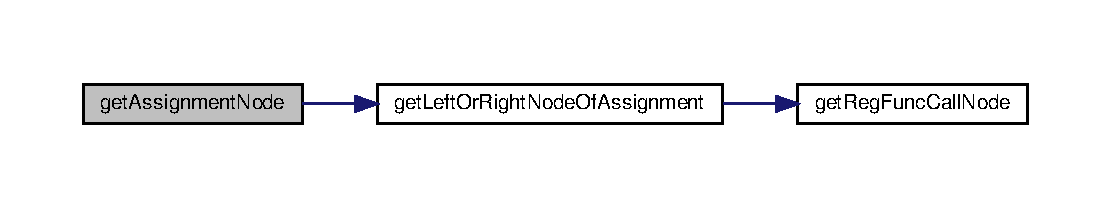
\includegraphics[width=350pt]{namespacePostProcessor_1_1astNodes_aa6c634c9a1dceb3e9cc65cadadf5f450_cgraph}
\end{center}
\end{figure}
Here is the caller graph for this function\+:\nopagebreak
\begin{figure}[H]
\begin{center}
\leavevmode
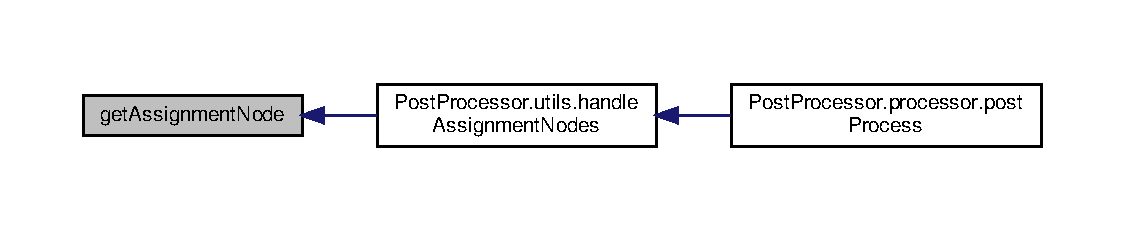
\includegraphics[width=350pt]{namespacePostProcessor_1_1astNodes_aa6c634c9a1dceb3e9cc65cadadf5f450_icgraph}
\end{center}
\end{figure}
\mbox{\Hypertarget{namespacePostProcessor_1_1astNodes_aebd6602b5bdafed24833f298500fd85c}\label{namespacePostProcessor_1_1astNodes_aebd6602b5bdafed24833f298500fd85c}} 
\index{Post\+Processor\+::ast\+Nodes@{Post\+Processor\+::ast\+Nodes}!get\+Declaration\+Node@{get\+Declaration\+Node}}
\index{get\+Declaration\+Node@{get\+Declaration\+Node}!Post\+Processor\+::ast\+Nodes@{Post\+Processor\+::ast\+Nodes}}
\subsubsection{\texorpdfstring{get\+Declaration\+Node()}{getDeclarationNode()}}
{\footnotesize\ttfamily def Post\+Processor.\+ast\+Nodes.\+get\+Declaration\+Node (\begin{DoxyParamCaption}\item[{}]{id\+Name }\end{DoxyParamCaption})}

\begin{DoxyVerb}Creates a declaration node for a variable with the specified name and the global type.

@param idName: The name of the variable to declare.
@type idName: str

@return: A `c_ast.Decl` node representing the variable declaration.
@rtype: c_ast.Decl
\end{DoxyVerb}
 

Definition at line 82 of file ast\+Nodes.\+py.


\begin{DoxyCode}
82 \textcolor{keyword}{def }\hyperlink{namespacePostProcessor_1_1astNodes_aebd6602b5bdafed24833f298500fd85c}{getDeclarationNode}(idName):
83     \textcolor{stringliteral}{"""
}
84 \textcolor{stringliteral}{    Creates a declaration node for a variable with the specified name and the global type.
}
85 \textcolor{stringliteral}{
}
86 \textcolor{stringliteral}{    @param idName: The name of the variable to declare.
}
87 \textcolor{stringliteral}{    @type idName: str
}
88 \textcolor{stringliteral}{
}
89 \textcolor{stringliteral}{    @return: A `c\_ast.Decl` node representing the variable declaration.
}
90 \textcolor{stringliteral}{    @rtype: c\_ast.Decl
}
91 \textcolor{stringliteral}{    """}
92     
93     \textcolor{comment}{# print(globalVariables.globalType)
}
94     typeDeclNode = c\_ast.TypeDecl(declname = idName,quals = [],align = \textcolor{keywordtype}{None},
95                                                 type=c\_ast.IdentifierType(names=[globalVariables.globalType
      ]))
96     declNode = c\_ast.Decl(name=idName, quals=[], storage=[], funcspec=[],
97                 type=typeDeclNode, init=\textcolor{keywordtype}{None},
98                 bitsize=\textcolor{keywordtype}{None}, align=[])
99     \textcolor{keywordflow}{return} declNode
\end{DoxyCode}
\mbox{\Hypertarget{namespacePostProcessor_1_1astNodes_afb1489449acb633bf78b48165fe578be}\label{namespacePostProcessor_1_1astNodes_afb1489449acb633bf78b48165fe578be}} 
\index{Post\+Processor\+::ast\+Nodes@{Post\+Processor\+::ast\+Nodes}!get\+Left\+Or\+Right\+Node\+Of\+Assignment@{get\+Left\+Or\+Right\+Node\+Of\+Assignment}}
\index{get\+Left\+Or\+Right\+Node\+Of\+Assignment@{get\+Left\+Or\+Right\+Node\+Of\+Assignment}!Post\+Processor\+::ast\+Nodes@{Post\+Processor\+::ast\+Nodes}}
\subsubsection{\texorpdfstring{get\+Left\+Or\+Right\+Node\+Of\+Assignment()}{getLeftOrRightNodeOfAssignment()}}
{\footnotesize\ttfamily def Post\+Processor.\+ast\+Nodes.\+get\+Left\+Or\+Right\+Node\+Of\+Assignment (\begin{DoxyParamCaption}\item[{}]{operand }\end{DoxyParamCaption})}

\begin{DoxyVerb}Generates the corresponding AST node for a given operand based on its type.

@param operand: The operand for which to create the AST node.
@type operand: str

@return: A `c_ast.ID`, `c_ast.UnaryOp`, or `c_ast.FuncCall` node based on the operand's prefix.
@rtype: c_ast.ID | c_ast.UnaryOp | c_ast.FuncCall
\end{DoxyVerb}
 

Definition at line 21 of file ast\+Nodes.\+py.


\begin{DoxyCode}
21 \textcolor{keyword}{def }\hyperlink{namespacePostProcessor_1_1astNodes_afb1489449acb633bf78b48165fe578be}{getLeftOrRightNodeOfAssignment}(operand):
22     \textcolor{stringliteral}{"""
}
23 \textcolor{stringliteral}{    Generates the corresponding AST node for a given operand based on its type.
}
24 \textcolor{stringliteral}{
}
25 \textcolor{stringliteral}{    @param operand: The operand for which to create the AST node.
}
26 \textcolor{stringliteral}{    @type operand: str
}
27 \textcolor{stringliteral}{
}
28 \textcolor{stringliteral}{    @return: A `c\_ast.ID`, `c\_ast.UnaryOp`, or `c\_ast.FuncCall` node based on the operand's prefix.
}
29 \textcolor{stringliteral}{    @rtype: c\_ast.ID | c\_ast.UnaryOp | c\_ast.FuncCall
}
30 \textcolor{stringliteral}{    """}
31     \textcolor{keywordflow}{if} operand.startswith(\textcolor{stringliteral}{"v\_reg"}):
32         node = \hyperlink{namespacePostProcessor_1_1astNodes_a30de65f8e1753733f88a01d42927ef1b}{getRegFuncCallNode}(operand[6:])
33     \textcolor{keywordflow}{elif} operand.startswith(\textcolor{stringliteral}{"v\_neg"}):
34             node = c\_ast.UnaryOp(op=\textcolor{stringliteral}{'!'},expr=c\_ast.ID(name=operand[6:]))
35     \textcolor{keywordflow}{else}:
36         node = c\_ast.ID(name=operand)
37     \textcolor{keywordflow}{return} node
38 
\end{DoxyCode}
Here is the call graph for this function\+:\nopagebreak
\begin{figure}[H]
\begin{center}
\leavevmode
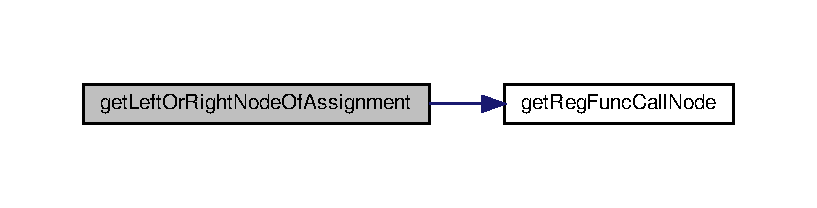
\includegraphics[width=350pt]{namespacePostProcessor_1_1astNodes_afb1489449acb633bf78b48165fe578be_cgraph}
\end{center}
\end{figure}
Here is the caller graph for this function\+:\nopagebreak
\begin{figure}[H]
\begin{center}
\leavevmode
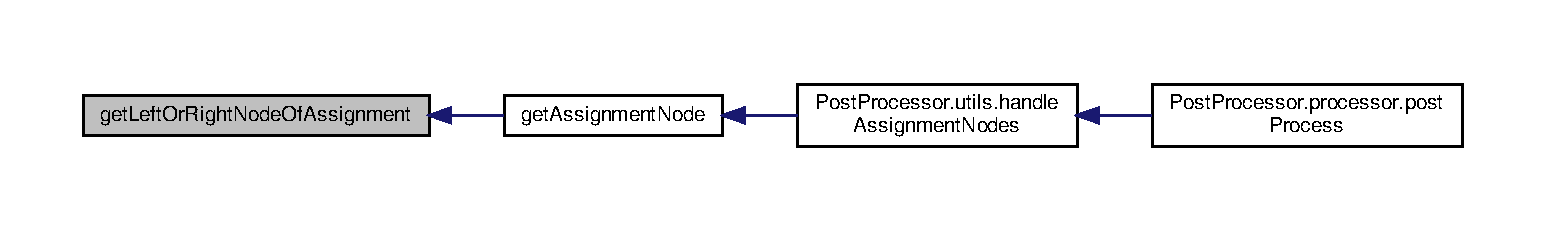
\includegraphics[width=350pt]{namespacePostProcessor_1_1astNodes_afb1489449acb633bf78b48165fe578be_icgraph}
\end{center}
\end{figure}
\mbox{\Hypertarget{namespacePostProcessor_1_1astNodes_a30de65f8e1753733f88a01d42927ef1b}\label{namespacePostProcessor_1_1astNodes_a30de65f8e1753733f88a01d42927ef1b}} 
\index{Post\+Processor\+::ast\+Nodes@{Post\+Processor\+::ast\+Nodes}!get\+Reg\+Func\+Call\+Node@{get\+Reg\+Func\+Call\+Node}}
\index{get\+Reg\+Func\+Call\+Node@{get\+Reg\+Func\+Call\+Node}!Post\+Processor\+::ast\+Nodes@{Post\+Processor\+::ast\+Nodes}}
\subsubsection{\texorpdfstring{get\+Reg\+Func\+Call\+Node()}{getRegFuncCallNode()}}
{\footnotesize\ttfamily def Post\+Processor.\+ast\+Nodes.\+get\+Reg\+Func\+Call\+Node (\begin{DoxyParamCaption}\item[{}]{name }\end{DoxyParamCaption})}

\begin{DoxyVerb}Creates a function call node for the 'reg' function with a given argument.

@param name: The argument name for the 'reg' function.
@type name: str

@return: A `c_ast.FuncCall` node representing a function call to 'reg' with the specified argument.
@rtype: c_ast.FuncCall
\end{DoxyVerb}
 

Definition at line 8 of file ast\+Nodes.\+py.


\begin{DoxyCode}
8 \textcolor{keyword}{def }\hyperlink{namespacePostProcessor_1_1astNodes_a30de65f8e1753733f88a01d42927ef1b}{getRegFuncCallNode}(name):
9     \textcolor{stringliteral}{"""
}
10 \textcolor{stringliteral}{    Creates a function call node for the 'reg' function with a given argument.
}
11 \textcolor{stringliteral}{
}
12 \textcolor{stringliteral}{    @param name: The argument name for the 'reg' function.
}
13 \textcolor{stringliteral}{    @type name: str
}
14 \textcolor{stringliteral}{
}
15 \textcolor{stringliteral}{    @return: A `c\_ast.FuncCall` node representing a function call to 'reg' with the specified argument.
}
16 \textcolor{stringliteral}{    @rtype: c\_ast.FuncCall
}
17 \textcolor{stringliteral}{    """}
18     node = c\_ast.FuncCall(name=c\_ast.ID(name=\textcolor{stringliteral}{'reg'}),args=c\_ast.ExprList(exprs=[c\_ast.ID(name=name)]))
19     \textcolor{keywordflow}{return} node
20 
\end{DoxyCode}
Here is the caller graph for this function\+:\nopagebreak
\begin{figure}[H]
\begin{center}
\leavevmode
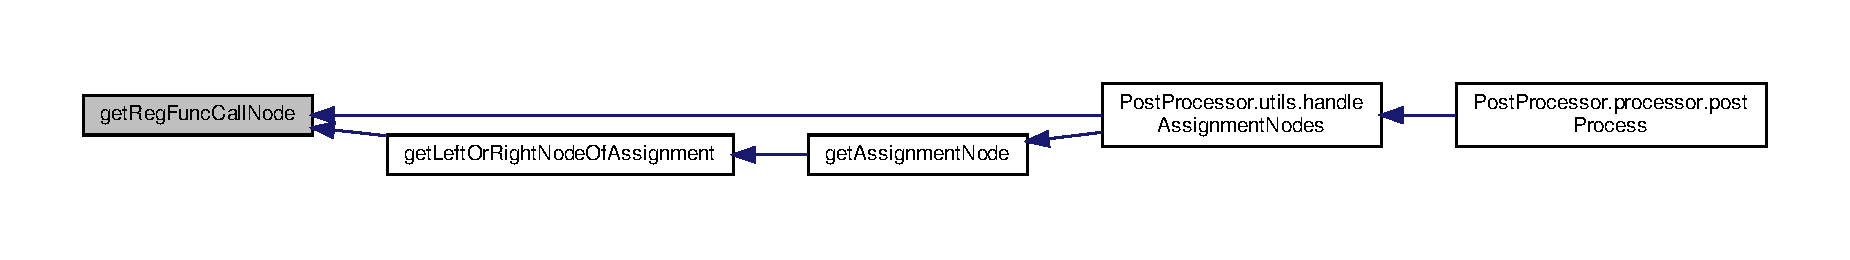
\includegraphics[width=350pt]{namespacePostProcessor_1_1astNodes_a30de65f8e1753733f88a01d42927ef1b_icgraph}
\end{center}
\end{figure}
\mbox{\Hypertarget{namespacePostProcessor_1_1astNodes_a1fc39a0ad420aefababe0a8ee2907f4e}\label{namespacePostProcessor_1_1astNodes_a1fc39a0ad420aefababe0a8ee2907f4e}} 
\index{Post\+Processor\+::ast\+Nodes@{Post\+Processor\+::ast\+Nodes}!get\+Simple\+Assignment\+Node@{get\+Simple\+Assignment\+Node}}
\index{get\+Simple\+Assignment\+Node@{get\+Simple\+Assignment\+Node}!Post\+Processor\+::ast\+Nodes@{Post\+Processor\+::ast\+Nodes}}
\subsubsection{\texorpdfstring{get\+Simple\+Assignment\+Node()}{getSimpleAssignmentNode()}}
{\footnotesize\ttfamily def Post\+Processor.\+ast\+Nodes.\+get\+Simple\+Assignment\+Node (\begin{DoxyParamCaption}\item[{}]{lvalue,  }\item[{}]{rvalue }\end{DoxyParamCaption})}

\begin{DoxyVerb}Creates a simple assignment node with the specified left-hand side and right-hand side.

@param lvalue: The left-hand side of the assignment.
@type lvalue: str
@param rvalue: The right-hand side of the assignment.
@type rvalue: c_ast.Node

@return: A `c_ast.Assignment` node representing the assignment operation.
@rtype: c_ast.Assignment
\end{DoxyVerb}
 

Definition at line 39 of file ast\+Nodes.\+py.


\begin{DoxyCode}
39 \textcolor{keyword}{def }\hyperlink{namespacePostProcessor_1_1astNodes_a1fc39a0ad420aefababe0a8ee2907f4e}{getSimpleAssignmentNode}(lvalue,rvalue):
40     \textcolor{stringliteral}{"""
}
41 \textcolor{stringliteral}{    Creates a simple assignment node with the specified left-hand side and right-hand side.
}
42 \textcolor{stringliteral}{
}
43 \textcolor{stringliteral}{    @param lvalue: The left-hand side of the assignment.
}
44 \textcolor{stringliteral}{    @type lvalue: str
}
45 \textcolor{stringliteral}{    @param rvalue: The right-hand side of the assignment.
}
46 \textcolor{stringliteral}{    @type rvalue: c\_ast.Node
}
47 \textcolor{stringliteral}{
}
48 \textcolor{stringliteral}{    @return: A `c\_ast.Assignment` node representing the assignment operation.
}
49 \textcolor{stringliteral}{    @rtype: c\_ast.Assignment
}
50 \textcolor{stringliteral}{    """}
51     \textcolor{keywordflow}{return} c\_ast.Assignment(op=\textcolor{stringliteral}{'='},lvalue=c\_ast.ID(name=lvalue),rvalue=rvalue)
52 
\end{DoxyCode}

\hypertarget{namespacePostProcessor_1_1globalVariables}{}\section{Post\+Processor.\+global\+Variables Namespace Reference}
\label{namespacePostProcessor_1_1globalVariables}\index{Post\+Processor.\+global\+Variables@{Post\+Processor.\+global\+Variables}}

\hypertarget{namespacePostProcessor_1_1processor}{}\section{Post\+Processor.\+processor Namespace Reference}
\label{namespacePostProcessor_1_1processor}\index{Post\+Processor.\+processor@{Post\+Processor.\+processor}}
\subsection*{Functions}
\begin{DoxyCompactItemize}
\item 
def \hyperlink{namespacePostProcessor_1_1processor_a3f18e4947e2313a8b23367f06f4b02c2}{post\+Process} (input\+File, output\+File)
\end{DoxyCompactItemize}
\subsection*{Variables}
\begin{DoxyCompactItemize}
\item 
\hyperlink{namespacePostProcessor_1_1processor_a8187411843a6284ffb964ef3fb9fcab3}{args} = json.\+load(file)
\item 
\hyperlink{namespacePostProcessor_1_1processor_a7e91ec681fdd5ff588de2f2d2c3dc3f6}{global\+Type}
\end{DoxyCompactItemize}


\subsection{Function Documentation}
\mbox{\Hypertarget{namespacePostProcessor_1_1processor_a3f18e4947e2313a8b23367f06f4b02c2}\label{namespacePostProcessor_1_1processor_a3f18e4947e2313a8b23367f06f4b02c2}} 
\index{Post\+Processor\+::processor@{Post\+Processor\+::processor}!post\+Process@{post\+Process}}
\index{post\+Process@{post\+Process}!Post\+Processor\+::processor@{Post\+Processor\+::processor}}
\subsubsection{\texorpdfstring{post\+Process()}{postProcess()}}
{\footnotesize\ttfamily def Post\+Processor.\+processor.\+post\+Process (\begin{DoxyParamCaption}\item[{}]{input\+File,  }\item[{}]{output\+File }\end{DoxyParamCaption})}

\begin{DoxyVerb}Processes the input C file, applies transformations, and generates the output C file.

@param inputFile: Path to the input C file to be processed.
@param outputFile: Path to the output C file where the processed code will be saved.

@raises FileNotFoundError: If the input file does not exist.
@raises IOError: If there is an issue with file reading or writing.
\end{DoxyVerb}
 

Definition at line 32 of file processor.\+py.


\begin{DoxyCode}
32 \textcolor{keyword}{def }\hyperlink{namespacePostProcessor_1_1processor_a3f18e4947e2313a8b23367f06f4b02c2}{postProcess}(inputFile,outputFile):
33     \textcolor{stringliteral}{"""
}
34 \textcolor{stringliteral}{    Processes the input C file, applies transformations, and generates the output C file.
}
35 \textcolor{stringliteral}{
}
36 \textcolor{stringliteral}{    @param inputFile: Path to the input C file to be processed.
}
37 \textcolor{stringliteral}{    @param outputFile: Path to the output C file where the processed code will be saved.
}
38 \textcolor{stringliteral}{
}
39 \textcolor{stringliteral}{    @raises FileNotFoundError: If the input file does not exist.
}
40 \textcolor{stringliteral}{    @raises IOError: If there is an issue with file reading or writing.
}
41 \textcolor{stringliteral}{    """}
42 
43     assgnNo = 1
44     ast = parse\_file(inputFile, use\_cpp=\textcolor{keyword}{True})
45     bodyNodes = []
46     with open(\textcolor{stringliteral}{'systemArgs.json'}, \textcolor{stringliteral}{'r') as file:
}
47 \textcolor{stringliteral}{        json\_data = file.read()
}
48 \textcolor{stringliteral}{    operatorNameMap = json.loads(json\_data)
}
49 \textcolor{stringliteral}{
}
50 \textcolor{stringliteral}{}\textcolor{comment}{#handling unary ops
}
51     negationVisitor = NegationVisitor(bodyNodes)
52     negationVisitor.visit(ast)
53     assgnNo = negationVisitor.assgnNo
54     ast.ext[0].body.block\_items = bodyNodes
55     bodyNodes = []
56 
57     unaryOpNodeChanger = UnaryOpNodeChanger(negationVisitor.unaryVarToNameMap)
58     unaryOpNodeChanger.visit(ast)
59 
60 \textcolor{comment}{#handling source regs
}
61     sourceRegHandler = SourceRegHandler(bodyNodes,assgnNo)
62     sourceRegHandler.visit(ast)
63     assgnNo = sourceRegHandler.assignNo
64     ast.ext[0].body.block\_items = bodyNodes
65     bodyNodes = []
66 
67 \textcolor{comment}{#handling nested reg binary op inside a reg call
}
68     binaryOpInRegHandler = BinaryOpInRegHandler(bodyNodes,assgnNo)
69     binaryOpInRegHandler.visit(ast)
70     assgnNo = binaryOpInRegHandler.assignNo
71     ast.ext[0].body.block\_items = bodyNodes
72     bodyNodes = []
73 
74 \textcolor{comment}{#handling nested reg binary op
}
75     \textcolor{keywordflow}{for} node \textcolor{keywordflow}{in} ast.ext[0].body.block\_items:
76         \textcolor{keywordflow}{if} \textcolor{keywordflow}{not} isinstance(node,c\_ast.Assignment):
77             bodyNodes.append(node)
78         \textcolor{keywordflow}{else}:
79             \hyperlink{namespacePostProcessor_1_1utils_a1ea8f909bf93721481e4fd1bd3f2dff1}{changeBinaryOps}(node,bodyNodes,assgnNo)
80             assgnNo += 2
81     ast.ext[0].body.block\_items = bodyNodes
82     \textcolor{comment}{# # print(ast)
}
83 
84     bodyNodes = []
85     \textcolor{keywordflow}{for} node \textcolor{keywordflow}{in} ast.ext[0].body.block\_items:
86         \textcolor{keywordflow}{if} \textcolor{keywordflow}{not} isinstance(node,c\_ast.Assignment):
87             bodyNodes.append(node)
88         \textcolor{keywordflow}{else}:
89             \hyperlink{namespacePostProcessor_1_1utils_a8b77a1f205d7dac14e6bdcccdb61e5f6}{handleAssignmentNodes}(node,bodyNodes,operatorNameMap,assgnNo)
90             assgnNo += 2
91     \textcolor{comment}{# print(bodyNodes)
}
92     ast.ext[0].body.block\_items = bodyNodes
93     \textcolor{comment}{# print(ast)
}
94     \hyperlink{namespaceutils_a5ab527c9affdfd39949f2e88c4299989}{generate\_c\_file}(ast,outputFile)
95 
96 
\end{DoxyCode}
Here is the call graph for this function\+:\nopagebreak
\begin{figure}[H]
\begin{center}
\leavevmode
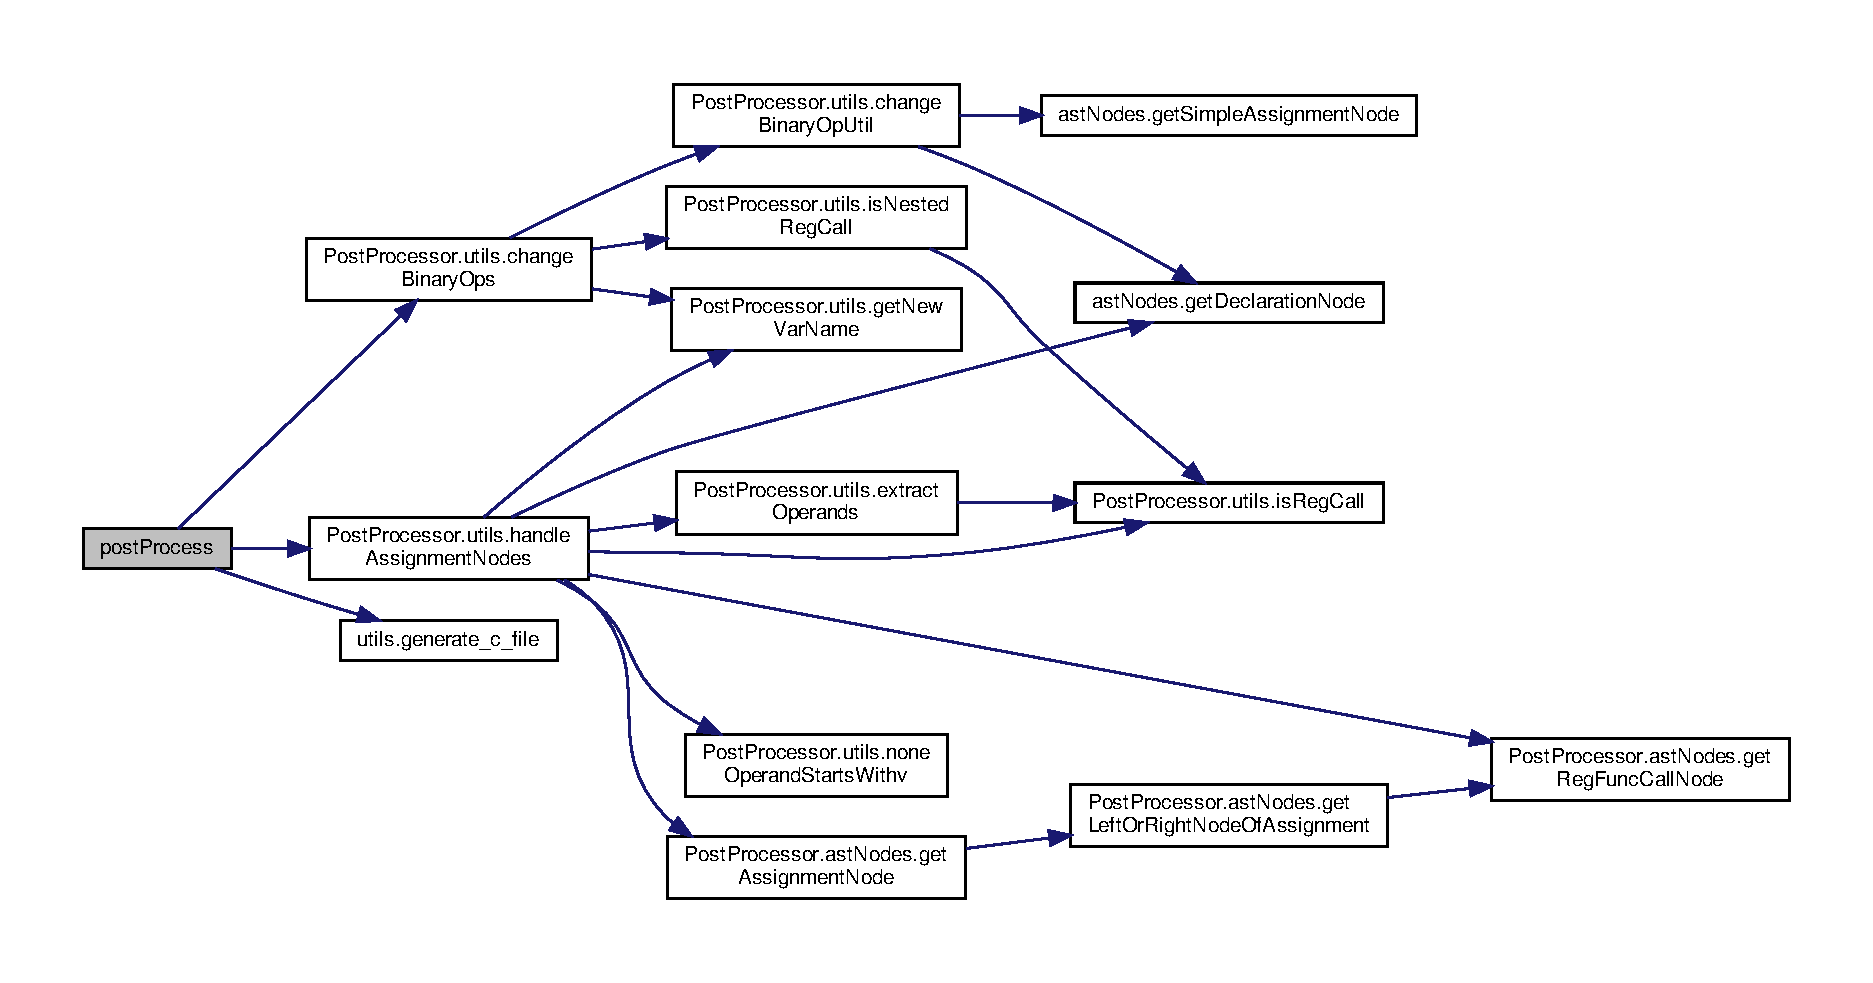
\includegraphics[width=350pt]{namespacePostProcessor_1_1processor_a3f18e4947e2313a8b23367f06f4b02c2_cgraph}
\end{center}
\end{figure}


\subsection{Variable Documentation}
\mbox{\Hypertarget{namespacePostProcessor_1_1processor_a8187411843a6284ffb964ef3fb9fcab3}\label{namespacePostProcessor_1_1processor_a8187411843a6284ffb964ef3fb9fcab3}} 
\index{Post\+Processor\+::processor@{Post\+Processor\+::processor}!args@{args}}
\index{args@{args}!Post\+Processor\+::processor@{Post\+Processor\+::processor}}
\subsubsection{\texorpdfstring{args}{args}}
{\footnotesize\ttfamily args = json.\+load(file)}



Definition at line 105 of file processor.\+py.

\mbox{\Hypertarget{namespacePostProcessor_1_1processor_a7e91ec681fdd5ff588de2f2d2c3dc3f6}\label{namespacePostProcessor_1_1processor_a7e91ec681fdd5ff588de2f2d2c3dc3f6}} 
\index{Post\+Processor\+::processor@{Post\+Processor\+::processor}!global\+Type@{global\+Type}}
\index{global\+Type@{global\+Type}!Post\+Processor\+::processor@{Post\+Processor\+::processor}}
\subsubsection{\texorpdfstring{global\+Type}{globalType}}
{\footnotesize\ttfamily global\+Type}



Definition at line 108 of file processor.\+py.


\hypertarget{namespacePostProcessor_1_1utils}{}\section{Post\+Processor.\+utils Namespace Reference}
\label{namespacePostProcessor_1_1utils}\index{Post\+Processor.\+utils@{Post\+Processor.\+utils}}
\subsection*{Functions}
\begin{DoxyCompactItemize}
\item 
def \hyperlink{namespacePostProcessor_1_1utils_a1ea8f909bf93721481e4fd1bd3f2dff1}{change\+Binary\+Ops} (node, body\+Nodes, assgn\+No)
\item 
def \hyperlink{namespacePostProcessor_1_1utils_ab12ae71cedd8ec3fcbfedd7a6dbe6599}{change\+Binary\+Op\+Util} (node, var\+For\+Binary\+Op, body\+Nodes)
\item 
def \hyperlink{namespacePostProcessor_1_1utils_a756305ef1f9ed9b8a0f01428433e026e}{extract\+Operands} (node)
\item 
def \hyperlink{namespacePostProcessor_1_1utils_a998fb471074ff747973a0d974eb9fbd1}{generate\+\_\+c\+\_\+file} (ast, filename)
\item 
def \hyperlink{namespacePostProcessor_1_1utils_a69c4094b747eccefbd43b8011b1c3626}{get\+New\+Var\+Name} (assgn\+No)
\item 
def \hyperlink{namespacePostProcessor_1_1utils_a9d9413cee00e1440bd03c215f3ebbaff}{get\+Variable\+Name\+From\+Operands} (operands, operator\+Name\+Map, operator=\char`\"{}\char`\"{})
\item 
def \hyperlink{namespacePostProcessor_1_1utils_a8b77a1f205d7dac14e6bdcccdb61e5f6}{handle\+Assignment\+Nodes} (node, body\+Nodes, operator\+Name\+Map, assgn\+No)
\item 
def \hyperlink{namespacePostProcessor_1_1utils_a86292ec94138d20acb13a3c9c136a468}{is\+Nested\+Reg\+Call} (node)
\item 
def \hyperlink{namespacePostProcessor_1_1utils_a89d6f2461251261de6b862c69fe3c44a}{is\+Reg\+Call} (node)
\item 
def \hyperlink{namespacePostProcessor_1_1utils_a379c264b5800e073d327d90d53cb854f}{none\+Operand\+Starts\+Withv} (operands)
\end{DoxyCompactItemize}


\subsection{Function Documentation}
\mbox{\Hypertarget{namespacePostProcessor_1_1utils_a1ea8f909bf93721481e4fd1bd3f2dff1}\label{namespacePostProcessor_1_1utils_a1ea8f909bf93721481e4fd1bd3f2dff1}} 
\index{Post\+Processor\+::utils@{Post\+Processor\+::utils}!change\+Binary\+Ops@{change\+Binary\+Ops}}
\index{change\+Binary\+Ops@{change\+Binary\+Ops}!Post\+Processor\+::utils@{Post\+Processor\+::utils}}
\subsubsection{\texorpdfstring{change\+Binary\+Ops()}{changeBinaryOps()}}
{\footnotesize\ttfamily def Post\+Processor.\+utils.\+change\+Binary\+Ops (\begin{DoxyParamCaption}\item[{}]{node,  }\item[{}]{body\+Nodes,  }\item[{}]{assgn\+No }\end{DoxyParamCaption})}

\begin{DoxyVerb}Modifies binary operations in the AST.

@param node: The node containing the binary operation to modify.
@param bodyNodes: The list of body nodes to append the modified nodes to.
@param assgnNo: The current assignment number used for generating new variable names.
\end{DoxyVerb}
 

Definition at line 114 of file utils.\+py.


\begin{DoxyCode}
114 \textcolor{keyword}{def }\hyperlink{namespacePostProcessor_1_1utils_a1ea8f909bf93721481e4fd1bd3f2dff1}{changeBinaryOps}(node,bodyNodes,assgnNo):
115     \textcolor{stringliteral}{"""
}
116 \textcolor{stringliteral}{    Modifies binary operations in the AST.
}
117 \textcolor{stringliteral}{
}
118 \textcolor{stringliteral}{    @param node: The node containing the binary operation to modify.
}
119 \textcolor{stringliteral}{    @param bodyNodes: The list of body nodes to append the modified nodes to.
}
120 \textcolor{stringliteral}{    @param assgnNo: The current assignment number used for generating new variable names.
}
121 \textcolor{stringliteral}{    """}
122     currNode = node.rvalue
123     \textcolor{keywordflow}{if} isinstance(currNode,c\_ast.BinaryOp):
124         origLeft = currNode.left
125         origRight = currNode.right
126         
127         \textcolor{keywordflow}{if} \hyperlink{namespacePostProcessor_1_1utils_a86292ec94138d20acb13a3c9c136a468}{isNestedRegCall}(currNode.right):
128             varForBinaryOp = \hyperlink{namespacePostProcessor_1_1utils_a69c4094b747eccefbd43b8011b1c3626}{getNewVarName}(assgnNo)
129             \hyperlink{namespacePostProcessor_1_1utils_ab12ae71cedd8ec3fcbfedd7a6dbe6599}{changeBinaryOpUtil}(currNode.right,varForBinaryOp,bodyNodes)
130             origRight = c\_ast.ID(varForBinaryOp)
131         \textcolor{keywordflow}{if} \hyperlink{namespacePostProcessor_1_1utils_a86292ec94138d20acb13a3c9c136a468}{isNestedRegCall}(currNode.left):
132             varForBinaryOp = \hyperlink{namespacePostProcessor_1_1utils_a69c4094b747eccefbd43b8011b1c3626}{getNewVarName}(assgnNo+1)
133             \hyperlink{namespacePostProcessor_1_1utils_ab12ae71cedd8ec3fcbfedd7a6dbe6599}{changeBinaryOpUtil}(currNode.left,varForBinaryOp,bodyNodes)
134             origLeft = c\_ast.ID(varForBinaryOp)
135         binaryOpNode = c\_ast.BinaryOp(op=currNode.op,left=origLeft,right=origRight)
136         bodyNodes.append(c\_ast.Assignment(op=\textcolor{stringliteral}{'='},lvalue=node.lvalue,rvalue=binaryOpNode))
137     \textcolor{keywordflow}{else}:
138         bodyNodes.append(node)
139 
\end{DoxyCode}
Here is the call graph for this function\+:\nopagebreak
\begin{figure}[H]
\begin{center}
\leavevmode
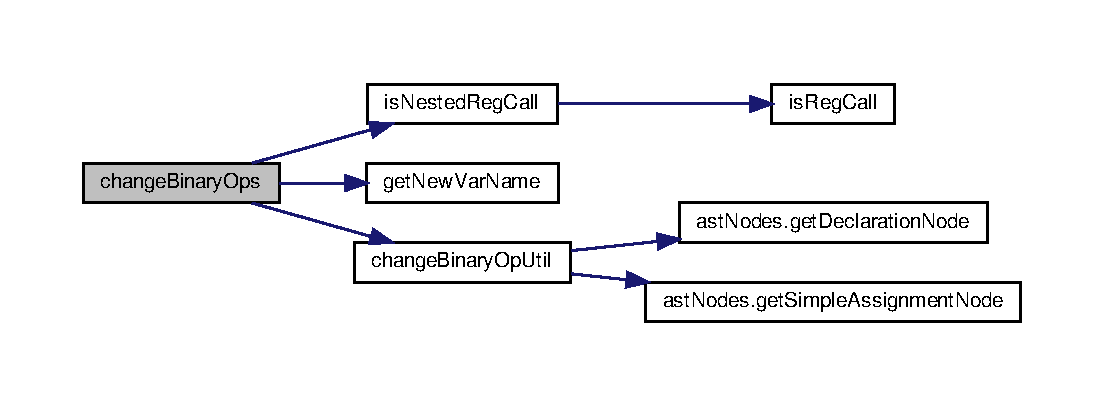
\includegraphics[width=350pt]{namespacePostProcessor_1_1utils_a1ea8f909bf93721481e4fd1bd3f2dff1_cgraph}
\end{center}
\end{figure}
Here is the caller graph for this function\+:\nopagebreak
\begin{figure}[H]
\begin{center}
\leavevmode
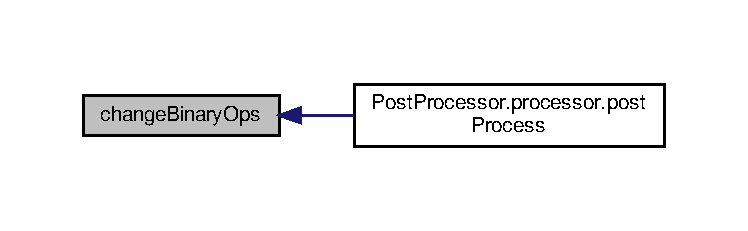
\includegraphics[width=350pt]{namespacePostProcessor_1_1utils_a1ea8f909bf93721481e4fd1bd3f2dff1_icgraph}
\end{center}
\end{figure}
\mbox{\Hypertarget{namespacePostProcessor_1_1utils_ab12ae71cedd8ec3fcbfedd7a6dbe6599}\label{namespacePostProcessor_1_1utils_ab12ae71cedd8ec3fcbfedd7a6dbe6599}} 
\index{Post\+Processor\+::utils@{Post\+Processor\+::utils}!change\+Binary\+Op\+Util@{change\+Binary\+Op\+Util}}
\index{change\+Binary\+Op\+Util@{change\+Binary\+Op\+Util}!Post\+Processor\+::utils@{Post\+Processor\+::utils}}
\subsubsection{\texorpdfstring{change\+Binary\+Op\+Util()}{changeBinaryOpUtil()}}
{\footnotesize\ttfamily def Post\+Processor.\+utils.\+change\+Binary\+Op\+Util (\begin{DoxyParamCaption}\item[{}]{node,  }\item[{}]{var\+For\+Binary\+Op,  }\item[{}]{body\+Nodes }\end{DoxyParamCaption})}

\begin{DoxyVerb}Utility function for changing binary operations.

@param node: The node representing the binary operation.
@param varForBinaryOp: The variable name for the binary operation.
@param bodyNodes: The list of body nodes to append the new nodes to.
\end{DoxyVerb}
 

Definition at line 103 of file utils.\+py.


\begin{DoxyCode}
103 \textcolor{keyword}{def }\hyperlink{namespacePostProcessor_1_1utils_ab12ae71cedd8ec3fcbfedd7a6dbe6599}{changeBinaryOpUtil}(node,varForBinaryOp,bodyNodes):
104     \textcolor{stringliteral}{"""
}
105 \textcolor{stringliteral}{    Utility function for changing binary operations.
}
106 \textcolor{stringliteral}{
}
107 \textcolor{stringliteral}{    @param node: The node representing the binary operation.
}
108 \textcolor{stringliteral}{    @param varForBinaryOp: The variable name for the binary operation.
}
109 \textcolor{stringliteral}{    @param bodyNodes: The list of body nodes to append the new nodes to.
}
110 \textcolor{stringliteral}{    """}
111     bodyNodes.append(\hyperlink{namespaceastNodes_ae5e5c7f09a1586002b20db6d72f6d30b}{getDeclarationNode}(varForBinaryOp))
112     bodyNodes.append(\hyperlink{namespaceastNodes_a2403f5d006e54f20e614226280cb6cbc}{getSimpleAssignmentNode}(varForBinaryOp,node))
113 
\end{DoxyCode}
Here is the call graph for this function\+:\nopagebreak
\begin{figure}[H]
\begin{center}
\leavevmode
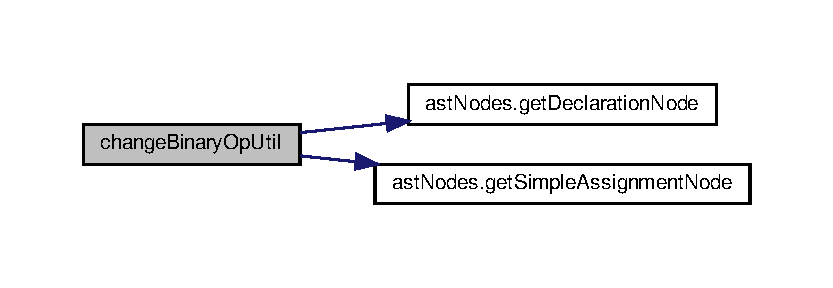
\includegraphics[width=350pt]{namespacePostProcessor_1_1utils_ab12ae71cedd8ec3fcbfedd7a6dbe6599_cgraph}
\end{center}
\end{figure}
Here is the caller graph for this function\+:\nopagebreak
\begin{figure}[H]
\begin{center}
\leavevmode
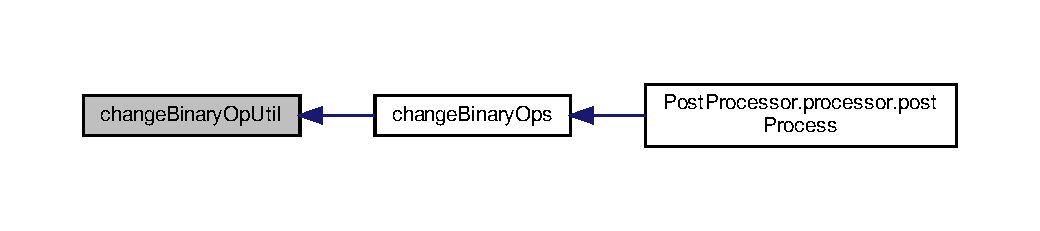
\includegraphics[width=350pt]{namespacePostProcessor_1_1utils_ab12ae71cedd8ec3fcbfedd7a6dbe6599_icgraph}
\end{center}
\end{figure}
\mbox{\Hypertarget{namespacePostProcessor_1_1utils_a756305ef1f9ed9b8a0f01428433e026e}\label{namespacePostProcessor_1_1utils_a756305ef1f9ed9b8a0f01428433e026e}} 
\index{Post\+Processor\+::utils@{Post\+Processor\+::utils}!extract\+Operands@{extract\+Operands}}
\index{extract\+Operands@{extract\+Operands}!Post\+Processor\+::utils@{Post\+Processor\+::utils}}
\subsubsection{\texorpdfstring{extract\+Operands()}{extractOperands()}}
{\footnotesize\ttfamily def Post\+Processor.\+utils.\+extract\+Operands (\begin{DoxyParamCaption}\item[{}]{node }\end{DoxyParamCaption})}

\begin{DoxyVerb}Extracts operands from a node, handling different node types.

@param node: The node from which to extract operands.

@return: A list of operands or a string representing the operand.
@raises ValueError: If the node type is unsupported.
\end{DoxyVerb}
 

Definition at line 43 of file utils.\+py.


\begin{DoxyCode}
43 \textcolor{keyword}{def }\hyperlink{namespacePostProcessor_1_1utils_a756305ef1f9ed9b8a0f01428433e026e}{extractOperands}(node):
44     \textcolor{stringliteral}{"""
}
45 \textcolor{stringliteral}{    Extracts operands from a node, handling different node types.
}
46 \textcolor{stringliteral}{
}
47 \textcolor{stringliteral}{    @param node: The node from which to extract operands.
}
48 \textcolor{stringliteral}{
}
49 \textcolor{stringliteral}{    @return: A list of operands or a string representing the operand.
}
50 \textcolor{stringliteral}{    @raises ValueError: If the node type is unsupported.
}
51 \textcolor{stringliteral}{    """}
52     \textcolor{keywordflow}{if} (isinstance(node, c\_ast.BinaryOp)):
53         leftOperand = \hyperlink{namespacePostProcessor_1_1utils_a756305ef1f9ed9b8a0f01428433e026e}{extractOperands}(node.left) 
54         rightOperand = \hyperlink{namespacePostProcessor_1_1utils_a756305ef1f9ed9b8a0f01428433e026e}{extractOperands}(node.right)
55         \textcolor{keywordflow}{return} [leftOperand,rightOperand]
56     \textcolor{keywordflow}{elif} \hyperlink{namespacePostProcessor_1_1utils_a89d6f2461251261de6b862c69fe3c44a}{isRegCall}(node):
57         \textcolor{keywordflow}{return} \textcolor{stringliteral}{"v\_reg\_"} + node.args.exprs[0].name
58     \textcolor{keywordflow}{elif} isinstance(node,c\_ast.ID):
59         \textcolor{keywordflow}{return} node.name
60     \textcolor{keywordflow}{elif} isinstance(node,c\_ast.UnaryOp):
61         \textcolor{keywordflow}{return} \textcolor{stringliteral}{"v\_neg\_"} + \hyperlink{namespacePostProcessor_1_1utils_a756305ef1f9ed9b8a0f01428433e026e}{extractOperands}(node.expr)
62     \textcolor{keywordflow}{else}:
63         \textcolor{keywordflow}{raise} ValueError(f\textcolor{stringliteral}{"Unsupported node type: \{type(node).\_\_name\_\_\}"})
64     
\end{DoxyCode}
Here is the call graph for this function\+:\nopagebreak
\begin{figure}[H]
\begin{center}
\leavevmode
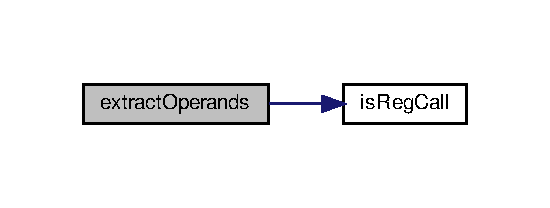
\includegraphics[width=264pt]{namespacePostProcessor_1_1utils_a756305ef1f9ed9b8a0f01428433e026e_cgraph}
\end{center}
\end{figure}
Here is the caller graph for this function\+:\nopagebreak
\begin{figure}[H]
\begin{center}
\leavevmode
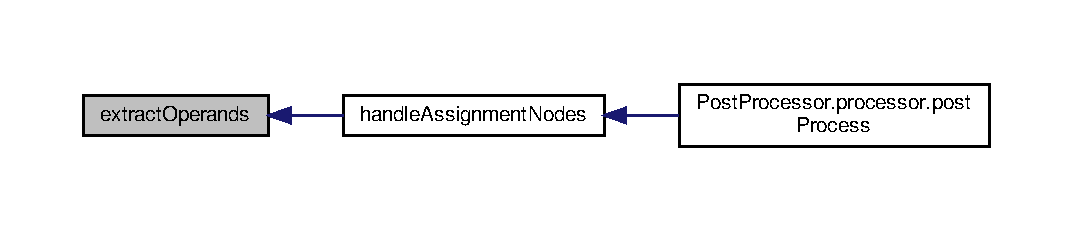
\includegraphics[width=350pt]{namespacePostProcessor_1_1utils_a756305ef1f9ed9b8a0f01428433e026e_icgraph}
\end{center}
\end{figure}
\mbox{\Hypertarget{namespacePostProcessor_1_1utils_a998fb471074ff747973a0d974eb9fbd1}\label{namespacePostProcessor_1_1utils_a998fb471074ff747973a0d974eb9fbd1}} 
\index{Post\+Processor\+::utils@{Post\+Processor\+::utils}!generate\+\_\+c\+\_\+file@{generate\+\_\+c\+\_\+file}}
\index{generate\+\_\+c\+\_\+file@{generate\+\_\+c\+\_\+file}!Post\+Processor\+::utils@{Post\+Processor\+::utils}}
\subsubsection{\texorpdfstring{generate\+\_\+c\+\_\+file()}{generate\_c\_file()}}
{\footnotesize\ttfamily def Post\+Processor.\+utils.\+generate\+\_\+c\+\_\+file (\begin{DoxyParamCaption}\item[{}]{ast,  }\item[{}]{filename }\end{DoxyParamCaption})}

\begin{DoxyVerb}Generates C code from the provided Abstract Syntax Tree (AST) and saves it to a file.

@param ast: The Abstract Syntax Tree (AST) to generate C code from.
@param filename: The path to the file where the generated C code will be saved.
\end{DoxyVerb}
 

Definition at line 140 of file utils.\+py.


\begin{DoxyCode}
140 \textcolor{keyword}{def }\hyperlink{namespacePostProcessor_1_1utils_a998fb471074ff747973a0d974eb9fbd1}{generate\_c\_file}(ast,filename):
141     \textcolor{stringliteral}{"""
}
142 \textcolor{stringliteral}{    Generates C code from the provided Abstract Syntax Tree (AST) and saves it to a file.
}
143 \textcolor{stringliteral}{
}
144 \textcolor{stringliteral}{    @param ast: The Abstract Syntax Tree (AST) to generate C code from.
}
145 \textcolor{stringliteral}{    @param filename: The path to the file where the generated C code will be saved.
}
146 \textcolor{stringliteral}{    """}
147     generator = c\_generator.CGenerator()
148     with open(filename, \textcolor{stringliteral}{'w'}) \textcolor{keyword}{as} output\_file:
149         print(generator.visit(ast), file=output\_file)
150 
151 
\end{DoxyCode}
\mbox{\Hypertarget{namespacePostProcessor_1_1utils_a69c4094b747eccefbd43b8011b1c3626}\label{namespacePostProcessor_1_1utils_a69c4094b747eccefbd43b8011b1c3626}} 
\index{Post\+Processor\+::utils@{Post\+Processor\+::utils}!get\+New\+Var\+Name@{get\+New\+Var\+Name}}
\index{get\+New\+Var\+Name@{get\+New\+Var\+Name}!Post\+Processor\+::utils@{Post\+Processor\+::utils}}
\subsubsection{\texorpdfstring{get\+New\+Var\+Name()}{getNewVarName()}}
{\footnotesize\ttfamily def Post\+Processor.\+utils.\+get\+New\+Var\+Name (\begin{DoxyParamCaption}\item[{}]{assgn\+No }\end{DoxyParamCaption})}

\begin{DoxyVerb}Generates a new variable name for assignments.

@param assgnNo: The assignment number to include in the variable name.

@return: A string representing the new variable name.
\end{DoxyVerb}
 

Definition at line 93 of file utils.\+py.


\begin{DoxyCode}
93 \textcolor{keyword}{def }\hyperlink{namespacePostProcessor_1_1utils_a69c4094b747eccefbd43b8011b1c3626}{getNewVarName}(assgnNo):
94     \textcolor{stringliteral}{"""
}
95 \textcolor{stringliteral}{    Generates a new variable name for assignments.
}
96 \textcolor{stringliteral}{
}
97 \textcolor{stringliteral}{    @param assgnNo: The assignment number to include in the variable name.
}
98 \textcolor{stringliteral}{
}
99 \textcolor{stringliteral}{    @return: A string representing the new variable name.
}
100 \textcolor{stringliteral}{    """}
101     \textcolor{keywordflow}{return} \textcolor{stringliteral}{"z"} + str(assgnNo) + \textcolor{stringliteral}{"\_assgn"} + str(assgnNo)
102 
\end{DoxyCode}
Here is the caller graph for this function\+:\nopagebreak
\begin{figure}[H]
\begin{center}
\leavevmode
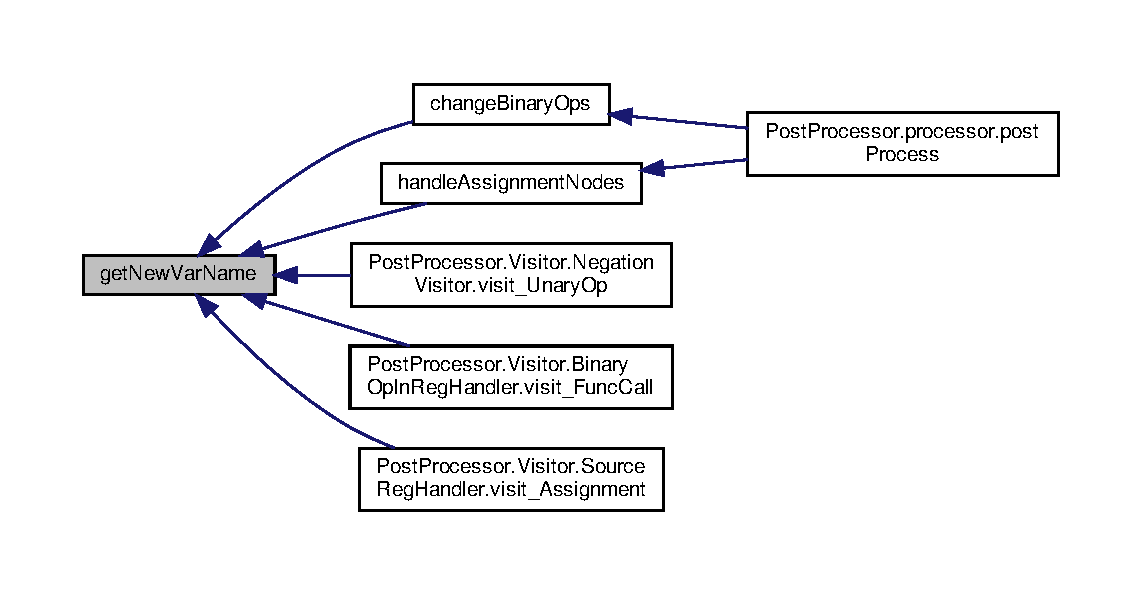
\includegraphics[width=350pt]{namespacePostProcessor_1_1utils_a69c4094b747eccefbd43b8011b1c3626_icgraph}
\end{center}
\end{figure}
\mbox{\Hypertarget{namespacePostProcessor_1_1utils_a9d9413cee00e1440bd03c215f3ebbaff}\label{namespacePostProcessor_1_1utils_a9d9413cee00e1440bd03c215f3ebbaff}} 
\index{Post\+Processor\+::utils@{Post\+Processor\+::utils}!get\+Variable\+Name\+From\+Operands@{get\+Variable\+Name\+From\+Operands}}
\index{get\+Variable\+Name\+From\+Operands@{get\+Variable\+Name\+From\+Operands}!Post\+Processor\+::utils@{Post\+Processor\+::utils}}
\subsubsection{\texorpdfstring{get\+Variable\+Name\+From\+Operands()}{getVariableNameFromOperands()}}
{\footnotesize\ttfamily def Post\+Processor.\+utils.\+get\+Variable\+Name\+From\+Operands (\begin{DoxyParamCaption}\item[{}]{operands,  }\item[{}]{operator\+Name\+Map,  }\item[{}]{operator = {\ttfamily \char`\"{}\char`\"{}} }\end{DoxyParamCaption})}

\begin{DoxyVerb}Constructs a variable name based on operands and operator.

@param operands: The list of operands.
@param operatorNameMap: A dictionary mapping operators to their names.
@param operator: The operator to include in the variable name.

@return: A string representing the variable name.
\end{DoxyVerb}
 

Definition at line 65 of file utils.\+py.


\begin{DoxyCode}
65 \textcolor{keyword}{def }\hyperlink{namespacePostProcessor_1_1utils_a9d9413cee00e1440bd03c215f3ebbaff}{getVariableNameFromOperands}(operands,operatorNameMap,operator = ""):
66     \textcolor{stringliteral}{"""
}
67 \textcolor{stringliteral}{    Constructs a variable name based on operands and operator.
}
68 \textcolor{stringliteral}{
}
69 \textcolor{stringliteral}{    @param operands: The list of operands.
}
70 \textcolor{stringliteral}{    @param operatorNameMap: A dictionary mapping operators to their names.
}
71 \textcolor{stringliteral}{    @param operator: The operator to include in the variable name.
}
72 \textcolor{stringliteral}{
}
73 \textcolor{stringliteral}{    @return: A string representing the variable name.
}
74 \textcolor{stringliteral}{    """}
75     variableName = operands[0]
76     if(len(operands) > 1):
77         variableName += (\textcolor{stringliteral}{"\_"} + operatorNameMap[operator] + \textcolor{stringliteral}{"\_"} + operands[1])
78     \textcolor{keywordflow}{return} variableName
79 
\end{DoxyCode}
\mbox{\Hypertarget{namespacePostProcessor_1_1utils_a8b77a1f205d7dac14e6bdcccdb61e5f6}\label{namespacePostProcessor_1_1utils_a8b77a1f205d7dac14e6bdcccdb61e5f6}} 
\index{Post\+Processor\+::utils@{Post\+Processor\+::utils}!handle\+Assignment\+Nodes@{handle\+Assignment\+Nodes}}
\index{handle\+Assignment\+Nodes@{handle\+Assignment\+Nodes}!Post\+Processor\+::utils@{Post\+Processor\+::utils}}
\subsubsection{\texorpdfstring{handle\+Assignment\+Nodes()}{handleAssignmentNodes()}}
{\footnotesize\ttfamily def Post\+Processor.\+utils.\+handle\+Assignment\+Nodes (\begin{DoxyParamCaption}\item[{}]{node,  }\item[{}]{body\+Nodes,  }\item[{}]{operator\+Name\+Map,  }\item[{}]{assgn\+No }\end{DoxyParamCaption})}

\begin{DoxyVerb}Processes and handles assignment nodes in the AST.

@param node: The assignment node to process.
@param bodyNodes: The list of body nodes to append the processed nodes to.
@param operatorNameMap: A dictionary mapping operators to their names.
@param assgnNo: The current assignment number used for generating new variable names.
\end{DoxyVerb}
 

Definition at line 152 of file utils.\+py.


\begin{DoxyCode}
152 \textcolor{keyword}{def }\hyperlink{namespacePostProcessor_1_1utils_a8b77a1f205d7dac14e6bdcccdb61e5f6}{handleAssignmentNodes}(node,bodyNodes,operatorNameMap,assgnNo):
153     \textcolor{stringliteral}{"""
}
154 \textcolor{stringliteral}{    Processes and handles assignment nodes in the AST.
}
155 \textcolor{stringliteral}{
}
156 \textcolor{stringliteral}{    @param node: The assignment node to process.
}
157 \textcolor{stringliteral}{    @param bodyNodes: The list of body nodes to append the processed nodes to.
}
158 \textcolor{stringliteral}{    @param operatorNameMap: A dictionary mapping operators to their names.
}
159 \textcolor{stringliteral}{    @param assgnNo: The current assignment number used for generating new variable names.
}
160 \textcolor{stringliteral}{    """}
161     count = 1;
162     currNode = node.rvalue
163     \textcolor{keywordflow}{if} \hyperlink{namespacePostProcessor_1_1utils_a89d6f2461251261de6b862c69fe3c44a}{isRegCall}(currNode):
164         \textcolor{keywordflow}{while} \hyperlink{namespacePostProcessor_1_1utils_a89d6f2461251261de6b862c69fe3c44a}{isRegCall}(currNode.args.exprs[0]):
165             count += 1
166             currNode = currNode.args.exprs[0]
167         currNode = currNode.args.exprs[0]
168         operands = \hyperlink{namespacePostProcessor_1_1utils_a756305ef1f9ed9b8a0f01428433e026e}{extractOperands}(currNode)
169         \textcolor{keywordflow}{if} \textcolor{keywordflow}{not} isinstance(operands,list):
170             operands = [operands]
171 
172         \textcolor{keywordflow}{if} count == 1 \textcolor{keywordflow}{and} \hyperlink{namespacePostProcessor_1_1utils_a379c264b5800e073d327d90d53cb854f}{noneOperandStartsWithv}(operands):
173              bodyNodes.append(node)
174              \textcolor{keywordflow}{return}
175 
176         op = currNode.op \textcolor{keywordflow}{if} isinstance(currNode, c\_ast.BinaryOp) \textcolor{keywordflow}{else} \textcolor{stringliteral}{""}
177         variableName = \hyperlink{namespacePostProcessor_1_1utils_a69c4094b747eccefbd43b8011b1c3626}{getNewVarName}(assgnNo)
178         assignmentNode = \hyperlink{namespacePostProcessor_1_1astNodes_aa6c634c9a1dceb3e9cc65cadadf5f450}{getAssignmentNode}(operands,op,variableName)
179         \textcolor{comment}{# if len(operands) > 1:
}
180         bodyNodes.append(\hyperlink{namespaceastNodes_ae5e5c7f09a1586002b20db6d72f6d30b}{getDeclarationNode}(variableName))
181         bodyNodes.append(assignmentNode)
182         prevVarName = variableName
183 
184         \textcolor{keywordflow}{for} index \textcolor{keywordflow}{in} range(count):
185             newVarName = variableName + str(index)
186             \textcolor{keywordflow}{if} index != count - 1:
187                 bodyNodes.append(\hyperlink{namespaceastNodes_ae5e5c7f09a1586002b20db6d72f6d30b}{getDeclarationNode}(newVarName))
188             regCallNode = \hyperlink{namespacePostProcessor_1_1astNodes_a30de65f8e1753733f88a01d42927ef1b}{getRegFuncCallNode}(prevVarName)
189             lvalue = c\_ast.ID(newVarName) \textcolor{keywordflow}{if} index != count -1 \textcolor{keywordflow}{else} node.lvalue
190             bodyNodes.append(c\_ast.Assignment(op=\textcolor{stringliteral}{'='},lvalue=lvalue,rvalue=regCallNode))
191             prevVarName = newVarName
192         
193     \textcolor{keywordflow}{else}:
194         bodyNodes.append(node)
195     
\end{DoxyCode}
Here is the call graph for this function\+:\nopagebreak
\begin{figure}[H]
\begin{center}
\leavevmode
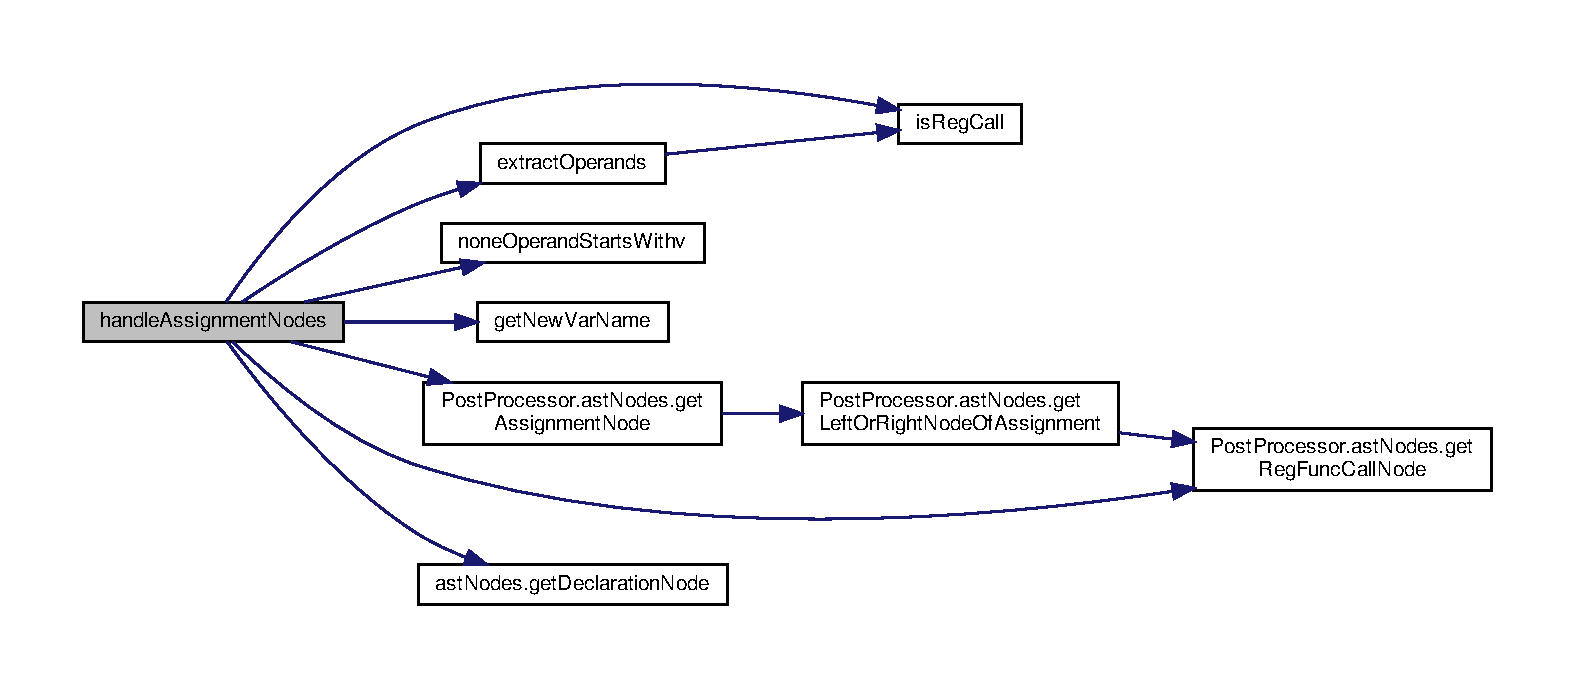
\includegraphics[width=350pt]{namespacePostProcessor_1_1utils_a8b77a1f205d7dac14e6bdcccdb61e5f6_cgraph}
\end{center}
\end{figure}
Here is the caller graph for this function\+:\nopagebreak
\begin{figure}[H]
\begin{center}
\leavevmode
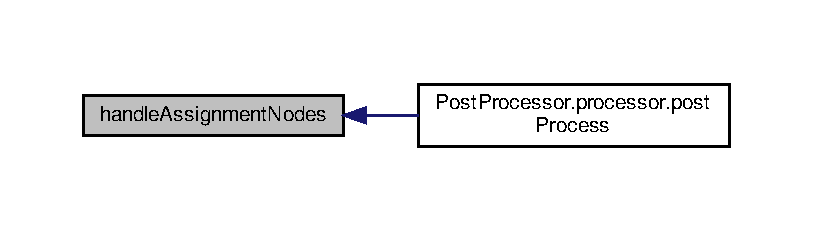
\includegraphics[width=350pt]{namespacePostProcessor_1_1utils_a8b77a1f205d7dac14e6bdcccdb61e5f6_icgraph}
\end{center}
\end{figure}
\mbox{\Hypertarget{namespacePostProcessor_1_1utils_a86292ec94138d20acb13a3c9c136a468}\label{namespacePostProcessor_1_1utils_a86292ec94138d20acb13a3c9c136a468}} 
\index{Post\+Processor\+::utils@{Post\+Processor\+::utils}!is\+Nested\+Reg\+Call@{is\+Nested\+Reg\+Call}}
\index{is\+Nested\+Reg\+Call@{is\+Nested\+Reg\+Call}!Post\+Processor\+::utils@{Post\+Processor\+::utils}}
\subsubsection{\texorpdfstring{is\+Nested\+Reg\+Call()}{isNestedRegCall()}}
{\footnotesize\ttfamily def Post\+Processor.\+utils.\+is\+Nested\+Reg\+Call (\begin{DoxyParamCaption}\item[{}]{node }\end{DoxyParamCaption})}

\begin{DoxyVerb}Checks if a node is a nested register function call.

@param node: The node to check.

@return: True if the node is a nested `reg` function call, False otherwise.
\end{DoxyVerb}
 

Definition at line 33 of file utils.\+py.


\begin{DoxyCode}
33 \textcolor{keyword}{def }\hyperlink{namespacePostProcessor_1_1utils_a86292ec94138d20acb13a3c9c136a468}{isNestedRegCall}(node):
34     \textcolor{stringliteral}{"""
}
35 \textcolor{stringliteral}{    Checks if a node is a nested register function call.
}
36 \textcolor{stringliteral}{
}
37 \textcolor{stringliteral}{    @param node: The node to check.
}
38 \textcolor{stringliteral}{
}
39 \textcolor{stringliteral}{    @return: True if the node is a nested `reg` function call, False otherwise.
}
40 \textcolor{stringliteral}{    """}
41     \textcolor{keywordflow}{return} \hyperlink{namespacePostProcessor_1_1utils_a89d6f2461251261de6b862c69fe3c44a}{isRegCall}(node) \textcolor{keywordflow}{and} \hyperlink{namespacePostProcessor_1_1utils_a89d6f2461251261de6b862c69fe3c44a}{isRegCall}(node.args.exprs[0])
42 
\end{DoxyCode}
Here is the call graph for this function\+:\nopagebreak
\begin{figure}[H]
\begin{center}
\leavevmode
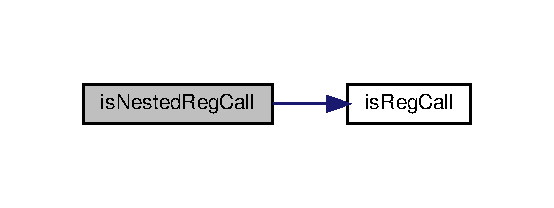
\includegraphics[width=266pt]{namespacePostProcessor_1_1utils_a86292ec94138d20acb13a3c9c136a468_cgraph}
\end{center}
\end{figure}
Here is the caller graph for this function\+:\nopagebreak
\begin{figure}[H]
\begin{center}
\leavevmode
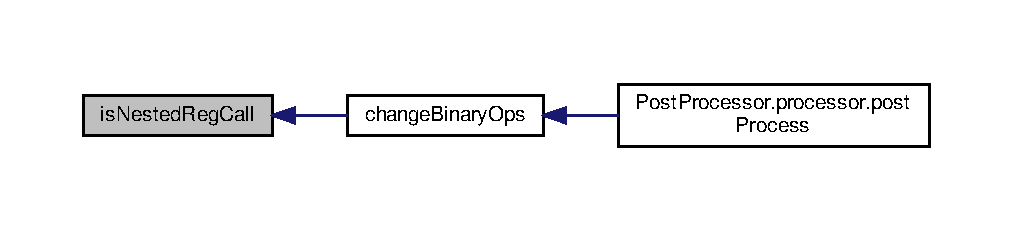
\includegraphics[width=350pt]{namespacePostProcessor_1_1utils_a86292ec94138d20acb13a3c9c136a468_icgraph}
\end{center}
\end{figure}
\mbox{\Hypertarget{namespacePostProcessor_1_1utils_a89d6f2461251261de6b862c69fe3c44a}\label{namespacePostProcessor_1_1utils_a89d6f2461251261de6b862c69fe3c44a}} 
\index{Post\+Processor\+::utils@{Post\+Processor\+::utils}!is\+Reg\+Call@{is\+Reg\+Call}}
\index{is\+Reg\+Call@{is\+Reg\+Call}!Post\+Processor\+::utils@{Post\+Processor\+::utils}}
\subsubsection{\texorpdfstring{is\+Reg\+Call()}{isRegCall()}}
{\footnotesize\ttfamily def Post\+Processor.\+utils.\+is\+Reg\+Call (\begin{DoxyParamCaption}\item[{}]{node }\end{DoxyParamCaption})}

\begin{DoxyVerb}Checks if a node represents a call to the "reg" function.

@param node: The node to check.

@return: True if the node is a `reg` function call, False otherwise.
\end{DoxyVerb}
 

Definition at line 23 of file utils.\+py.


\begin{DoxyCode}
23 \textcolor{keyword}{def }\hyperlink{namespacePostProcessor_1_1utils_a89d6f2461251261de6b862c69fe3c44a}{isRegCall}(node):
24     \textcolor{stringliteral}{"""
}
25 \textcolor{stringliteral}{    Checks if a node represents a call to the "reg" function.
}
26 \textcolor{stringliteral}{
}
27 \textcolor{stringliteral}{    @param node: The node to check.
}
28 \textcolor{stringliteral}{
}
29 \textcolor{stringliteral}{    @return: True if the node is a `reg` function call, False otherwise.
}
30 \textcolor{stringliteral}{    """}
31     \textcolor{keywordflow}{return} isinstance(node,c\_ast.FuncCall) \textcolor{keywordflow}{and} node.name.name == \textcolor{stringliteral}{'reg'}
32 
\end{DoxyCode}
Here is the caller graph for this function\+:\nopagebreak
\begin{figure}[H]
\begin{center}
\leavevmode
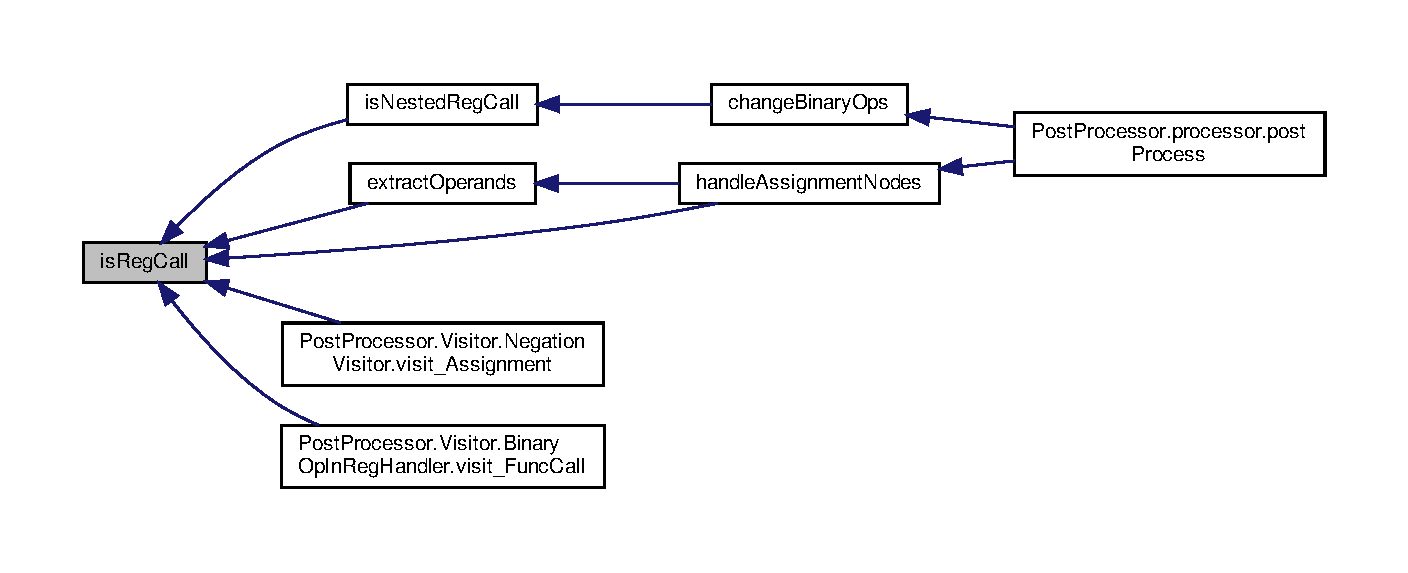
\includegraphics[width=350pt]{namespacePostProcessor_1_1utils_a89d6f2461251261de6b862c69fe3c44a_icgraph}
\end{center}
\end{figure}
\mbox{\Hypertarget{namespacePostProcessor_1_1utils_a379c264b5800e073d327d90d53cb854f}\label{namespacePostProcessor_1_1utils_a379c264b5800e073d327d90d53cb854f}} 
\index{Post\+Processor\+::utils@{Post\+Processor\+::utils}!none\+Operand\+Starts\+Withv@{none\+Operand\+Starts\+Withv}}
\index{none\+Operand\+Starts\+Withv@{none\+Operand\+Starts\+Withv}!Post\+Processor\+::utils@{Post\+Processor\+::utils}}
\subsubsection{\texorpdfstring{none\+Operand\+Starts\+Withv()}{noneOperandStartsWithv()}}
{\footnotesize\ttfamily def Post\+Processor.\+utils.\+none\+Operand\+Starts\+Withv (\begin{DoxyParamCaption}\item[{}]{operands }\end{DoxyParamCaption})}

\begin{DoxyVerb}Checks if none of the operands start with 'v'.

@param operands: The list of operands.

@return: True if none of the operands start with 'v', False otherwise.
\end{DoxyVerb}
 

Definition at line 80 of file utils.\+py.


\begin{DoxyCode}
80 \textcolor{keyword}{def }\hyperlink{namespacePostProcessor_1_1utils_a379c264b5800e073d327d90d53cb854f}{noneOperandStartsWithv}(operands):
81     \textcolor{stringliteral}{"""
}
82 \textcolor{stringliteral}{    Checks if none of the operands start with 'v'.
}
83 \textcolor{stringliteral}{
}
84 \textcolor{stringliteral}{    @param operands: The list of operands.
}
85 \textcolor{stringliteral}{
}
86 \textcolor{stringliteral}{    @return: True if none of the operands start with 'v', False otherwise.
}
87 \textcolor{stringliteral}{    """}
88     \textcolor{keywordflow}{for} operand \textcolor{keywordflow}{in} operands:
89         \textcolor{keywordflow}{if} operand.startswith(\textcolor{stringliteral}{"v"}):
90             \textcolor{keywordflow}{return} \textcolor{keyword}{False}
91     \textcolor{keywordflow}{return} \textcolor{keyword}{True}
92 
\end{DoxyCode}
Here is the caller graph for this function\+:\nopagebreak
\begin{figure}[H]
\begin{center}
\leavevmode
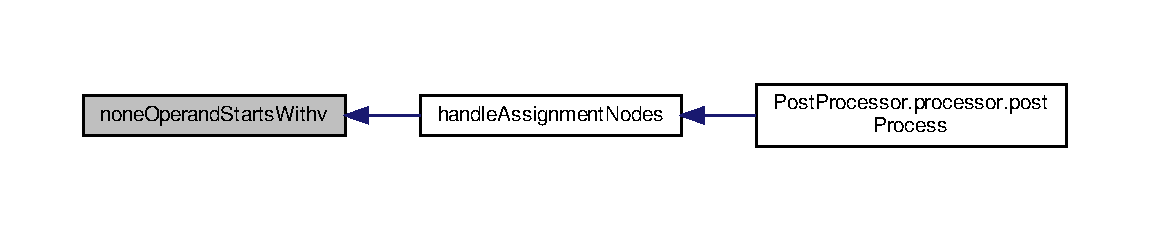
\includegraphics[width=350pt]{namespacePostProcessor_1_1utils_a379c264b5800e073d327d90d53cb854f_icgraph}
\end{center}
\end{figure}

\hypertarget{namespacePostProcessor_1_1Visitor}{}\section{Post\+Processor.\+Visitor Namespace Reference}
\label{namespacePostProcessor_1_1Visitor}\index{Post\+Processor.\+Visitor@{Post\+Processor.\+Visitor}}
\subsection*{Classes}
\begin{DoxyCompactItemize}
\item 
class \hyperlink{classPostProcessor_1_1Visitor_1_1BinaryOpInRegHandler}{Binary\+Op\+In\+Reg\+Handler}
\item 
class \hyperlink{classPostProcessor_1_1Visitor_1_1NegationVisitor}{Negation\+Visitor}
\item 
class \hyperlink{classPostProcessor_1_1Visitor_1_1SourceRegHandler}{Source\+Reg\+Handler}
\item 
class \hyperlink{classPostProcessor_1_1Visitor_1_1UnaryOpNodeChanger}{Unary\+Op\+Node\+Changer}
\end{DoxyCompactItemize}

\hypertarget{namespaceRegBalancer}{}\section{Reg\+Balancer Namespace Reference}
\label{namespaceRegBalancer}\index{Reg\+Balancer@{Reg\+Balancer}}
\subsection*{Namespaces}
\begin{DoxyCompactItemize}
\item 
 \hyperlink{namespaceRegBalancer_1_1src}{src}
\end{DoxyCompactItemize}

\hypertarget{namespaceRegBalancer_1_1src}{}\section{Reg\+Balancer.\+src Namespace Reference}
\label{namespaceRegBalancer_1_1src}\index{Reg\+Balancer.\+src@{Reg\+Balancer.\+src}}
\subsection*{Namespaces}
\begin{DoxyCompactItemize}
\item 
 \hyperlink{namespaceRegBalancer_1_1src_1_1composibility}{composibility}
\item 
 \hyperlink{namespaceRegBalancer_1_1src_1_1main}{main}
\item 
 \hyperlink{namespaceRegBalancer_1_1src_1_1test__retiming}{test\+\_\+retiming}
\end{DoxyCompactItemize}

\hypertarget{namespaceRegBalancer_1_1src_1_1composibility}{}\section{Reg\+Balancer.\+src.\+composibility Namespace Reference}
\label{namespaceRegBalancer_1_1src_1_1composibility}\index{Reg\+Balancer.\+src.\+composibility@{Reg\+Balancer.\+src.\+composibility}}
\subsection*{Variables}
\begin{DoxyCompactItemize}
\item 
\hyperlink{namespaceRegBalancer_1_1src_1_1composibility_a66fdaaee4f1e3923f619ce48cda79c4b}{all\+\_\+functions} = ast.\+ext
\item 
\hyperlink{namespaceRegBalancer_1_1src_1_1composibility_a83d838e3813fb5999c0492e0d9474bd9}{ast} = parse\+\_\+file(\hyperlink{namespaceRegBalancer_1_1src_1_1composibility_ad0ede32ef292a83cc0fde90bb81978c4}{filepath}, use\+\_\+cpp=False)
\item 
\hyperlink{namespaceRegBalancer_1_1src_1_1composibility_aef6cb15d000f3eb44586433c8b067068}{block\+\_\+items}
\item 
\hyperlink{namespaceRegBalancer_1_1src_1_1composibility_a3f696370e9fad0f95d9d7fef40cf2bcc}{c\+\_\+gen} = c\+\_\+generator.\+C\+Generator()
\item 
\hyperlink{namespaceRegBalancer_1_1src_1_1composibility_ac5c76c0448d4b265e8faf0bd0319ed41}{declname}
\item 
\hyperlink{namespaceRegBalancer_1_1src_1_1composibility_a40a5d58ffa6e88aa578d6683ac413105}{file}
\item 
string \hyperlink{namespaceRegBalancer_1_1src_1_1composibility_ad0ede32ef292a83cc0fde90bb81978c4}{filepath} = \textquotesingle{}../test/composibility/mult4.\+c\textquotesingle{}
\item 
list \hyperlink{namespaceRegBalancer_1_1src_1_1composibility_ab591e3ac73982297a6110aac7105546f}{func\+\_\+call\+\_\+outputs} = \mbox{[}$\,$\mbox{]}
\item 
\hyperlink{namespaceRegBalancer_1_1src_1_1composibility_a2ca84f740f9f5532d08ce6706ab8c818}{func\+\_\+def} = \hyperlink{namespaceRegBalancer_1_1src_1_1composibility_a66fdaaee4f1e3923f619ce48cda79c4b}{all\+\_\+functions}\mbox{[}0\mbox{]}
\item 
\hyperlink{namespaceRegBalancer_1_1src_1_1composibility_a204f446339af7929852f44df41484be5}{lhs} = line.\+lvalue
\item 
\hyperlink{namespaceRegBalancer_1_1src_1_1composibility_ab74e6bf80237ddc4109968cedc58c151}{name}
\item 
list \hyperlink{namespaceRegBalancer_1_1src_1_1composibility_a8ad9b335145f9b7a76cc1e6e2423cf0c}{new\+\_\+block\+\_\+items} = \mbox{[}$\,$\mbox{]}
\item 
\hyperlink{namespaceRegBalancer_1_1src_1_1composibility_a1653f591881c9ae74c9113cd4af0e30f}{new\+\_\+decl} = deepcopy(\hyperlink{namespaceRegBalancer_1_1src_1_1composibility_a3993b1a481d9e52328b2399c5ec6c791}{type\+\_\+decl}\mbox{[}arg.\+name\mbox{]})
\item 
string \hyperlink{namespaceRegBalancer_1_1src_1_1composibility_aa6afe46260181a45f14175dd7c70dc5e}{new\+\_\+filepath} = f\char`\"{}\{filepath\mbox{[}\+:-\/2\mbox{]}\}\+\_\+output.\+c\char`\"{}
\item 
\hyperlink{namespaceRegBalancer_1_1src_1_1composibility_ac7f01b5df0ebd2339035b77990cda224}{rhs} = line.\+rvalue
\item 
\hyperlink{namespaceRegBalancer_1_1src_1_1composibility_ac08a79afda9b81d9c7649a4d2134905f}{rslt} = c\+\_\+gen.\+visit(\hyperlink{namespaceRegBalancer_1_1src_1_1composibility_a83d838e3813fb5999c0492e0d9474bd9}{ast})
\item 
dictionary \hyperlink{namespaceRegBalancer_1_1src_1_1composibility_a3993b1a481d9e52328b2399c5ec6c791}{type\+\_\+decl} = \{\}
\end{DoxyCompactItemize}


\subsection{Variable Documentation}
\mbox{\Hypertarget{namespaceRegBalancer_1_1src_1_1composibility_a66fdaaee4f1e3923f619ce48cda79c4b}\label{namespaceRegBalancer_1_1src_1_1composibility_a66fdaaee4f1e3923f619ce48cda79c4b}} 
\index{Reg\+Balancer\+::src\+::composibility@{Reg\+Balancer\+::src\+::composibility}!all\+\_\+functions@{all\+\_\+functions}}
\index{all\+\_\+functions@{all\+\_\+functions}!Reg\+Balancer\+::src\+::composibility@{Reg\+Balancer\+::src\+::composibility}}
\subsubsection{\texorpdfstring{all\+\_\+functions}{all\_functions}}
{\footnotesize\ttfamily all\+\_\+functions = ast.\+ext}



Definition at line 24 of file composibility.\+py.

\mbox{\Hypertarget{namespaceRegBalancer_1_1src_1_1composibility_a83d838e3813fb5999c0492e0d9474bd9}\label{namespaceRegBalancer_1_1src_1_1composibility_a83d838e3813fb5999c0492e0d9474bd9}} 
\index{Reg\+Balancer\+::src\+::composibility@{Reg\+Balancer\+::src\+::composibility}!ast@{ast}}
\index{ast@{ast}!Reg\+Balancer\+::src\+::composibility@{Reg\+Balancer\+::src\+::composibility}}
\subsubsection{\texorpdfstring{ast}{ast}}
{\footnotesize\ttfamily ast = parse\+\_\+file(\hyperlink{namespaceRegBalancer_1_1src_1_1composibility_ad0ede32ef292a83cc0fde90bb81978c4}{filepath}, use\+\_\+cpp=False)}



Definition at line 23 of file composibility.\+py.

\mbox{\Hypertarget{namespaceRegBalancer_1_1src_1_1composibility_aef6cb15d000f3eb44586433c8b067068}\label{namespaceRegBalancer_1_1src_1_1composibility_aef6cb15d000f3eb44586433c8b067068}} 
\index{Reg\+Balancer\+::src\+::composibility@{Reg\+Balancer\+::src\+::composibility}!block\+\_\+items@{block\+\_\+items}}
\index{block\+\_\+items@{block\+\_\+items}!Reg\+Balancer\+::src\+::composibility@{Reg\+Balancer\+::src\+::composibility}}
\subsubsection{\texorpdfstring{block\+\_\+items}{block\_items}}
{\footnotesize\ttfamily block\+\_\+items}



Definition at line 48 of file composibility.\+py.

\mbox{\Hypertarget{namespaceRegBalancer_1_1src_1_1composibility_a3f696370e9fad0f95d9d7fef40cf2bcc}\label{namespaceRegBalancer_1_1src_1_1composibility_a3f696370e9fad0f95d9d7fef40cf2bcc}} 
\index{Reg\+Balancer\+::src\+::composibility@{Reg\+Balancer\+::src\+::composibility}!c\+\_\+gen@{c\+\_\+gen}}
\index{c\+\_\+gen@{c\+\_\+gen}!Reg\+Balancer\+::src\+::composibility@{Reg\+Balancer\+::src\+::composibility}}
\subsubsection{\texorpdfstring{c\+\_\+gen}{c\_gen}}
{\footnotesize\ttfamily c\+\_\+gen = c\+\_\+generator.\+C\+Generator()}



Definition at line 49 of file composibility.\+py.

\mbox{\Hypertarget{namespaceRegBalancer_1_1src_1_1composibility_ac5c76c0448d4b265e8faf0bd0319ed41}\label{namespaceRegBalancer_1_1src_1_1composibility_ac5c76c0448d4b265e8faf0bd0319ed41}} 
\index{Reg\+Balancer\+::src\+::composibility@{Reg\+Balancer\+::src\+::composibility}!declname@{declname}}
\index{declname@{declname}!Reg\+Balancer\+::src\+::composibility@{Reg\+Balancer\+::src\+::composibility}}
\subsubsection{\texorpdfstring{declname}{declname}}
{\footnotesize\ttfamily declname}



Definition at line 40 of file composibility.\+py.

\mbox{\Hypertarget{namespaceRegBalancer_1_1src_1_1composibility_a40a5d58ffa6e88aa578d6683ac413105}\label{namespaceRegBalancer_1_1src_1_1composibility_a40a5d58ffa6e88aa578d6683ac413105}} 
\index{Reg\+Balancer\+::src\+::composibility@{Reg\+Balancer\+::src\+::composibility}!file@{file}}
\index{file@{file}!Reg\+Balancer\+::src\+::composibility@{Reg\+Balancer\+::src\+::composibility}}
\subsubsection{\texorpdfstring{file}{file}}
{\footnotesize\ttfamily file}



Definition at line 53 of file composibility.\+py.

\mbox{\Hypertarget{namespaceRegBalancer_1_1src_1_1composibility_ad0ede32ef292a83cc0fde90bb81978c4}\label{namespaceRegBalancer_1_1src_1_1composibility_ad0ede32ef292a83cc0fde90bb81978c4}} 
\index{Reg\+Balancer\+::src\+::composibility@{Reg\+Balancer\+::src\+::composibility}!filepath@{filepath}}
\index{filepath@{filepath}!Reg\+Balancer\+::src\+::composibility@{Reg\+Balancer\+::src\+::composibility}}
\subsubsection{\texorpdfstring{filepath}{filepath}}
{\footnotesize\ttfamily string filepath = \textquotesingle{}../test/composibility/mult4.\+c\textquotesingle{}}



Definition at line 22 of file composibility.\+py.

\mbox{\Hypertarget{namespaceRegBalancer_1_1src_1_1composibility_ab591e3ac73982297a6110aac7105546f}\label{namespaceRegBalancer_1_1src_1_1composibility_ab591e3ac73982297a6110aac7105546f}} 
\index{Reg\+Balancer\+::src\+::composibility@{Reg\+Balancer\+::src\+::composibility}!func\+\_\+call\+\_\+outputs@{func\+\_\+call\+\_\+outputs}}
\index{func\+\_\+call\+\_\+outputs@{func\+\_\+call\+\_\+outputs}!Reg\+Balancer\+::src\+::composibility@{Reg\+Balancer\+::src\+::composibility}}
\subsubsection{\texorpdfstring{func\+\_\+call\+\_\+outputs}{func\_call\_outputs}}
{\footnotesize\ttfamily list func\+\_\+call\+\_\+outputs = \mbox{[}$\,$\mbox{]}}



Definition at line 26 of file composibility.\+py.

\mbox{\Hypertarget{namespaceRegBalancer_1_1src_1_1composibility_a2ca84f740f9f5532d08ce6706ab8c818}\label{namespaceRegBalancer_1_1src_1_1composibility_a2ca84f740f9f5532d08ce6706ab8c818}} 
\index{Reg\+Balancer\+::src\+::composibility@{Reg\+Balancer\+::src\+::composibility}!func\+\_\+def@{func\+\_\+def}}
\index{func\+\_\+def@{func\+\_\+def}!Reg\+Balancer\+::src\+::composibility@{Reg\+Balancer\+::src\+::composibility}}
\subsubsection{\texorpdfstring{func\+\_\+def}{func\_def}}
{\footnotesize\ttfamily func\+\_\+def = \hyperlink{namespaceRegBalancer_1_1src_1_1composibility_a66fdaaee4f1e3923f619ce48cda79c4b}{all\+\_\+functions}\mbox{[}0\mbox{]}}



Definition at line 25 of file composibility.\+py.

\mbox{\Hypertarget{namespaceRegBalancer_1_1src_1_1composibility_a204f446339af7929852f44df41484be5}\label{namespaceRegBalancer_1_1src_1_1composibility_a204f446339af7929852f44df41484be5}} 
\index{Reg\+Balancer\+::src\+::composibility@{Reg\+Balancer\+::src\+::composibility}!lhs@{lhs}}
\index{lhs@{lhs}!Reg\+Balancer\+::src\+::composibility@{Reg\+Balancer\+::src\+::composibility}}
\subsubsection{\texorpdfstring{lhs}{lhs}}
{\footnotesize\ttfamily lhs = line.\+lvalue}



Definition at line 33 of file composibility.\+py.

\mbox{\Hypertarget{namespaceRegBalancer_1_1src_1_1composibility_ab74e6bf80237ddc4109968cedc58c151}\label{namespaceRegBalancer_1_1src_1_1composibility_ab74e6bf80237ddc4109968cedc58c151}} 
\index{Reg\+Balancer\+::src\+::composibility@{Reg\+Balancer\+::src\+::composibility}!name@{name}}
\index{name@{name}!Reg\+Balancer\+::src\+::composibility@{Reg\+Balancer\+::src\+::composibility}}
\subsubsection{\texorpdfstring{name}{name}}
{\footnotesize\ttfamily name}



Definition at line 44 of file composibility.\+py.

\mbox{\Hypertarget{namespaceRegBalancer_1_1src_1_1composibility_a8ad9b335145f9b7a76cc1e6e2423cf0c}\label{namespaceRegBalancer_1_1src_1_1composibility_a8ad9b335145f9b7a76cc1e6e2423cf0c}} 
\index{Reg\+Balancer\+::src\+::composibility@{Reg\+Balancer\+::src\+::composibility}!new\+\_\+block\+\_\+items@{new\+\_\+block\+\_\+items}}
\index{new\+\_\+block\+\_\+items@{new\+\_\+block\+\_\+items}!Reg\+Balancer\+::src\+::composibility@{Reg\+Balancer\+::src\+::composibility}}
\subsubsection{\texorpdfstring{new\+\_\+block\+\_\+items}{new\_block\_items}}
{\footnotesize\ttfamily list new\+\_\+block\+\_\+items = \mbox{[}$\,$\mbox{]}}



Definition at line 27 of file composibility.\+py.

\mbox{\Hypertarget{namespaceRegBalancer_1_1src_1_1composibility_a1653f591881c9ae74c9113cd4af0e30f}\label{namespaceRegBalancer_1_1src_1_1composibility_a1653f591881c9ae74c9113cd4af0e30f}} 
\index{Reg\+Balancer\+::src\+::composibility@{Reg\+Balancer\+::src\+::composibility}!new\+\_\+decl@{new\+\_\+decl}}
\index{new\+\_\+decl@{new\+\_\+decl}!Reg\+Balancer\+::src\+::composibility@{Reg\+Balancer\+::src\+::composibility}}
\subsubsection{\texorpdfstring{new\+\_\+decl}{new\_decl}}
{\footnotesize\ttfamily new\+\_\+decl = deepcopy(\hyperlink{namespaceRegBalancer_1_1src_1_1composibility_a3993b1a481d9e52328b2399c5ec6c791}{type\+\_\+decl}\mbox{[}arg.\+name\mbox{]})}



Definition at line 39 of file composibility.\+py.

\mbox{\Hypertarget{namespaceRegBalancer_1_1src_1_1composibility_aa6afe46260181a45f14175dd7c70dc5e}\label{namespaceRegBalancer_1_1src_1_1composibility_aa6afe46260181a45f14175dd7c70dc5e}} 
\index{Reg\+Balancer\+::src\+::composibility@{Reg\+Balancer\+::src\+::composibility}!new\+\_\+filepath@{new\+\_\+filepath}}
\index{new\+\_\+filepath@{new\+\_\+filepath}!Reg\+Balancer\+::src\+::composibility@{Reg\+Balancer\+::src\+::composibility}}
\subsubsection{\texorpdfstring{new\+\_\+filepath}{new\_filepath}}
{\footnotesize\ttfamily string new\+\_\+filepath = f\char`\"{}\{filepath\mbox{[}\+:-\/2\mbox{]}\}\+\_\+output.\+c\char`\"{}}



Definition at line 51 of file composibility.\+py.

\mbox{\Hypertarget{namespaceRegBalancer_1_1src_1_1composibility_ac7f01b5df0ebd2339035b77990cda224}\label{namespaceRegBalancer_1_1src_1_1composibility_ac7f01b5df0ebd2339035b77990cda224}} 
\index{Reg\+Balancer\+::src\+::composibility@{Reg\+Balancer\+::src\+::composibility}!rhs@{rhs}}
\index{rhs@{rhs}!Reg\+Balancer\+::src\+::composibility@{Reg\+Balancer\+::src\+::composibility}}
\subsubsection{\texorpdfstring{rhs}{rhs}}
{\footnotesize\ttfamily rhs = line.\+rvalue}



Definition at line 34 of file composibility.\+py.

\mbox{\Hypertarget{namespaceRegBalancer_1_1src_1_1composibility_ac08a79afda9b81d9c7649a4d2134905f}\label{namespaceRegBalancer_1_1src_1_1composibility_ac08a79afda9b81d9c7649a4d2134905f}} 
\index{Reg\+Balancer\+::src\+::composibility@{Reg\+Balancer\+::src\+::composibility}!rslt@{rslt}}
\index{rslt@{rslt}!Reg\+Balancer\+::src\+::composibility@{Reg\+Balancer\+::src\+::composibility}}
\subsubsection{\texorpdfstring{rslt}{rslt}}
{\footnotesize\ttfamily rslt = c\+\_\+gen.\+visit(\hyperlink{namespaceRegBalancer_1_1src_1_1composibility_a83d838e3813fb5999c0492e0d9474bd9}{ast})}



Definition at line 50 of file composibility.\+py.

\mbox{\Hypertarget{namespaceRegBalancer_1_1src_1_1composibility_a3993b1a481d9e52328b2399c5ec6c791}\label{namespaceRegBalancer_1_1src_1_1composibility_a3993b1a481d9e52328b2399c5ec6c791}} 
\index{Reg\+Balancer\+::src\+::composibility@{Reg\+Balancer\+::src\+::composibility}!type\+\_\+decl@{type\+\_\+decl}}
\index{type\+\_\+decl@{type\+\_\+decl}!Reg\+Balancer\+::src\+::composibility@{Reg\+Balancer\+::src\+::composibility}}
\subsubsection{\texorpdfstring{type\+\_\+decl}{type\_decl}}
{\footnotesize\ttfamily dictionary type\+\_\+decl = \{\}}



Definition at line 28 of file composibility.\+py.


\hypertarget{namespaceRegBalancer_1_1src_1_1main}{}\section{Reg\+Balancer.\+src.\+main Namespace Reference}
\label{namespaceRegBalancer_1_1src_1_1main}\index{Reg\+Balancer.\+src.\+main@{Reg\+Balancer.\+src.\+main}}
\subsection*{Variables}
\begin{DoxyCompactItemize}
\item 
\hyperlink{namespaceRegBalancer_1_1src_1_1main_a8187411843a6284ffb964ef3fb9fcab3}{args} = json.\+load(file)
\item 
\hyperlink{namespaceRegBalancer_1_1src_1_1main_a83d838e3813fb5999c0492e0d9474bd9}{ast} = parse\+\_\+file(\hyperlink{namespaceRegBalancer_1_1src_1_1main_a7b981d9b48acf5de0d1fefa71978ce4a}{file\+To\+Parse}, use\+\_\+cpp=True)
\item 
\hyperlink{namespaceRegBalancer_1_1src_1_1main_aa5d70a518fbbc3f1e03d57deb06db2e4}{dfg\+\_\+gen} = Generate\+D\+FG()
\item 
\hyperlink{namespaceRegBalancer_1_1src_1_1main_afb358f48b1646c750fb9da6c6585be2b}{end}
\item 
\hyperlink{namespaceRegBalancer_1_1src_1_1main_a7b981d9b48acf5de0d1fefa71978ce4a}{file\+To\+Parse} = \hyperlink{namespaceRegBalancer_1_1src_1_1main_a8187411843a6284ffb964ef3fb9fcab3}{args}\mbox{[}\char`\"{}post\+Processor\+Output\char`\"{}\mbox{]} if(\hyperlink{namespaceRegBalancer_1_1src_1_1main_a8187411843a6284ffb964ef3fb9fcab3}{args}\mbox{[}\char`\"{}check\+Balancing\char`\"{}\mbox{]}) else \hyperlink{namespaceRegBalancer_1_1src_1_1main_a8187411843a6284ffb964ef3fb9fcab3}{args}\mbox{[}\char`\"{}inliner\+Output\char`\"{}\mbox{]}
\item 
\hyperlink{namespaceRegBalancer_1_1src_1_1main_a6f1918359d19ff0f2ae80e155c83c951}{func\+\_\+body} = extract\+\_\+func\+\_\+body(\hyperlink{namespaceRegBalancer_1_1src_1_1main_a83d838e3813fb5999c0492e0d9474bd9}{ast})
\item 
\hyperlink{namespaceRegBalancer_1_1src_1_1main_aa9c65458d6900b176c9ff9b1ef34bed0}{manual\+Registers} = no\+Of\+Registers\+Manually(dfg\+\_\+gen.\+dfg)
\item 
\hyperlink{namespaceRegBalancer_1_1src_1_1main_a1209559bbc0dbee87e2e3044b791a287}{retimer} = Retime\+D\+FG(dfg\+\_\+gen.\+dfg)
\item 
\hyperlink{namespaceRegBalancer_1_1src_1_1main_a2530c3908f0179486a4c2255f792e27a}{start\+\_\+time} = time.\+time()
\item 
string \hyperlink{namespaceRegBalancer_1_1src_1_1main_a8feea255809654e1028144a6b312c9e8}{use\+Linear\+Algo} = \char`\"{}true\char`\"{}
\end{DoxyCompactItemize}


\subsection{Variable Documentation}
\mbox{\Hypertarget{namespaceRegBalancer_1_1src_1_1main_a8187411843a6284ffb964ef3fb9fcab3}\label{namespaceRegBalancer_1_1src_1_1main_a8187411843a6284ffb964ef3fb9fcab3}} 
\index{Reg\+Balancer\+::src\+::main@{Reg\+Balancer\+::src\+::main}!args@{args}}
\index{args@{args}!Reg\+Balancer\+::src\+::main@{Reg\+Balancer\+::src\+::main}}
\subsubsection{\texorpdfstring{args}{args}}
{\footnotesize\ttfamily args = json.\+load(file)}



Definition at line 45 of file main.\+py.

\mbox{\Hypertarget{namespaceRegBalancer_1_1src_1_1main_a83d838e3813fb5999c0492e0d9474bd9}\label{namespaceRegBalancer_1_1src_1_1main_a83d838e3813fb5999c0492e0d9474bd9}} 
\index{Reg\+Balancer\+::src\+::main@{Reg\+Balancer\+::src\+::main}!ast@{ast}}
\index{ast@{ast}!Reg\+Balancer\+::src\+::main@{Reg\+Balancer\+::src\+::main}}
\subsubsection{\texorpdfstring{ast}{ast}}
{\footnotesize\ttfamily ast = parse\+\_\+file(\hyperlink{namespaceRegBalancer_1_1src_1_1main_a7b981d9b48acf5de0d1fefa71978ce4a}{file\+To\+Parse}, use\+\_\+cpp=True)}



Definition at line 49 of file main.\+py.

\mbox{\Hypertarget{namespaceRegBalancer_1_1src_1_1main_aa5d70a518fbbc3f1e03d57deb06db2e4}\label{namespaceRegBalancer_1_1src_1_1main_aa5d70a518fbbc3f1e03d57deb06db2e4}} 
\index{Reg\+Balancer\+::src\+::main@{Reg\+Balancer\+::src\+::main}!dfg\+\_\+gen@{dfg\+\_\+gen}}
\index{dfg\+\_\+gen@{dfg\+\_\+gen}!Reg\+Balancer\+::src\+::main@{Reg\+Balancer\+::src\+::main}}
\subsubsection{\texorpdfstring{dfg\+\_\+gen}{dfg\_gen}}
{\footnotesize\ttfamily dfg\+\_\+gen = Generate\+D\+FG()}



Definition at line 52 of file main.\+py.

\mbox{\Hypertarget{namespaceRegBalancer_1_1src_1_1main_afb358f48b1646c750fb9da6c6585be2b}\label{namespaceRegBalancer_1_1src_1_1main_afb358f48b1646c750fb9da6c6585be2b}} 
\index{Reg\+Balancer\+::src\+::main@{Reg\+Balancer\+::src\+::main}!end@{end}}
\index{end@{end}!Reg\+Balancer\+::src\+::main@{Reg\+Balancer\+::src\+::main}}
\subsubsection{\texorpdfstring{end}{end}}
{\footnotesize\ttfamily end}



Definition at line 77 of file main.\+py.

\mbox{\Hypertarget{namespaceRegBalancer_1_1src_1_1main_a7b981d9b48acf5de0d1fefa71978ce4a}\label{namespaceRegBalancer_1_1src_1_1main_a7b981d9b48acf5de0d1fefa71978ce4a}} 
\index{Reg\+Balancer\+::src\+::main@{Reg\+Balancer\+::src\+::main}!file\+To\+Parse@{file\+To\+Parse}}
\index{file\+To\+Parse@{file\+To\+Parse}!Reg\+Balancer\+::src\+::main@{Reg\+Balancer\+::src\+::main}}
\subsubsection{\texorpdfstring{file\+To\+Parse}{fileToParse}}
{\footnotesize\ttfamily file\+To\+Parse = \hyperlink{namespaceRegBalancer_1_1src_1_1main_a8187411843a6284ffb964ef3fb9fcab3}{args}\mbox{[}\char`\"{}post\+Processor\+Output\char`\"{}\mbox{]} if(\hyperlink{namespaceRegBalancer_1_1src_1_1main_a8187411843a6284ffb964ef3fb9fcab3}{args}\mbox{[}\char`\"{}check\+Balancing\char`\"{}\mbox{]}) else \hyperlink{namespaceRegBalancer_1_1src_1_1main_a8187411843a6284ffb964ef3fb9fcab3}{args}\mbox{[}\char`\"{}inliner\+Output\char`\"{}\mbox{]}}



Definition at line 48 of file main.\+py.

\mbox{\Hypertarget{namespaceRegBalancer_1_1src_1_1main_a6f1918359d19ff0f2ae80e155c83c951}\label{namespaceRegBalancer_1_1src_1_1main_a6f1918359d19ff0f2ae80e155c83c951}} 
\index{Reg\+Balancer\+::src\+::main@{Reg\+Balancer\+::src\+::main}!func\+\_\+body@{func\+\_\+body}}
\index{func\+\_\+body@{func\+\_\+body}!Reg\+Balancer\+::src\+::main@{Reg\+Balancer\+::src\+::main}}
\subsubsection{\texorpdfstring{func\+\_\+body}{func\_body}}
{\footnotesize\ttfamily func\+\_\+body = extract\+\_\+func\+\_\+body(\hyperlink{namespaceRegBalancer_1_1src_1_1main_a83d838e3813fb5999c0492e0d9474bd9}{ast})}



Definition at line 50 of file main.\+py.

\mbox{\Hypertarget{namespaceRegBalancer_1_1src_1_1main_aa9c65458d6900b176c9ff9b1ef34bed0}\label{namespaceRegBalancer_1_1src_1_1main_aa9c65458d6900b176c9ff9b1ef34bed0}} 
\index{Reg\+Balancer\+::src\+::main@{Reg\+Balancer\+::src\+::main}!manual\+Registers@{manual\+Registers}}
\index{manual\+Registers@{manual\+Registers}!Reg\+Balancer\+::src\+::main@{Reg\+Balancer\+::src\+::main}}
\subsubsection{\texorpdfstring{manual\+Registers}{manualRegisters}}
{\footnotesize\ttfamily manual\+Registers = no\+Of\+Registers\+Manually(dfg\+\_\+gen.\+dfg)}



Definition at line 63 of file main.\+py.

\mbox{\Hypertarget{namespaceRegBalancer_1_1src_1_1main_a1209559bbc0dbee87e2e3044b791a287}\label{namespaceRegBalancer_1_1src_1_1main_a1209559bbc0dbee87e2e3044b791a287}} 
\index{Reg\+Balancer\+::src\+::main@{Reg\+Balancer\+::src\+::main}!retimer@{retimer}}
\index{retimer@{retimer}!Reg\+Balancer\+::src\+::main@{Reg\+Balancer\+::src\+::main}}
\subsubsection{\texorpdfstring{retimer}{retimer}}
{\footnotesize\ttfamily retimer = Retime\+D\+FG(dfg\+\_\+gen.\+dfg)}



Definition at line 69 of file main.\+py.

\mbox{\Hypertarget{namespaceRegBalancer_1_1src_1_1main_a2530c3908f0179486a4c2255f792e27a}\label{namespaceRegBalancer_1_1src_1_1main_a2530c3908f0179486a4c2255f792e27a}} 
\index{Reg\+Balancer\+::src\+::main@{Reg\+Balancer\+::src\+::main}!start\+\_\+time@{start\+\_\+time}}
\index{start\+\_\+time@{start\+\_\+time}!Reg\+Balancer\+::src\+::main@{Reg\+Balancer\+::src\+::main}}
\subsubsection{\texorpdfstring{start\+\_\+time}{start\_time}}
{\footnotesize\ttfamily start\+\_\+time = time.\+time()}



Definition at line 47 of file main.\+py.

\mbox{\Hypertarget{namespaceRegBalancer_1_1src_1_1main_a8feea255809654e1028144a6b312c9e8}\label{namespaceRegBalancer_1_1src_1_1main_a8feea255809654e1028144a6b312c9e8}} 
\index{Reg\+Balancer\+::src\+::main@{Reg\+Balancer\+::src\+::main}!use\+Linear\+Algo@{use\+Linear\+Algo}}
\index{use\+Linear\+Algo@{use\+Linear\+Algo}!Reg\+Balancer\+::src\+::main@{Reg\+Balancer\+::src\+::main}}
\subsubsection{\texorpdfstring{use\+Linear\+Algo}{useLinearAlgo}}
{\footnotesize\ttfamily string use\+Linear\+Algo = \char`\"{}true\char`\"{}}



Definition at line 68 of file main.\+py.


\hypertarget{namespaceRegBalancer_1_1src_1_1test__retiming}{}\section{Reg\+Balancer.\+src.\+test\+\_\+retiming Namespace Reference}
\label{namespaceRegBalancer_1_1src_1_1test__retiming}\index{Reg\+Balancer.\+src.\+test\+\_\+retiming@{Reg\+Balancer.\+src.\+test\+\_\+retiming}}
\subsection*{Variables}
\begin{DoxyCompactItemize}
\item 
\hyperlink{namespaceRegBalancer_1_1src_1_1test__retiming_a8d509c28896865f8640f328f30f15721}{dfg} = rx.\+Py\+Di\+Graph()
\item 
\hyperlink{namespaceRegBalancer_1_1src_1_1test__retiming_a64aa603bc3c6c1587e7c6542452481ac}{fig} = graphviz\+\_\+draw(\hyperlink{namespaceRegBalancer_1_1src_1_1test__retiming_a8d509c28896865f8640f328f30f15721}{dfg}, node\+\_\+attr\+\_\+fn=lambda n\+: \{\char`\"{}label\char`\"{}\+: n.\+label()\})
\item 
\hyperlink{namespaceRegBalancer_1_1src_1_1test__retiming_a9932f6d3a67f65e538d7ae56541a85da}{node1} = dfg.\+add\+\_\+node(Text\+Graph\+Node(\char`\"{}Source\char`\"{}))
\item 
\hyperlink{namespaceRegBalancer_1_1src_1_1test__retiming_a6f72570c732db7d8ffbb64f7eef9dea3}{node2} = dfg.\+add\+\_\+node(Text\+Graph\+Node(\char`\"{}Sink\char`\"{}))
\item 
\hyperlink{namespaceRegBalancer_1_1src_1_1test__retiming_a18dee1ca5dda5195c4e2e7f663a3a1dd}{node3} = dfg.\+add\+\_\+node(Text\+Graph\+Node(\char`\"{}3\char`\"{}, 1))
\item 
\hyperlink{namespaceRegBalancer_1_1src_1_1test__retiming_a5a06a6e27e760a838df9849e283cdb4c}{node4} = dfg.\+add\+\_\+node(Text\+Graph\+Node(\char`\"{}4\char`\"{}))
\item 
\hyperlink{namespaceRegBalancer_1_1src_1_1test__retiming_ae47890d9ef0dda045dc2824bd221ff36}{node5} = dfg.\+add\+\_\+node(Text\+Graph\+Node(\char`\"{}Dummy\char`\"{}, 1))
\item 
\hyperlink{namespaceRegBalancer_1_1src_1_1test__retiming_a1209559bbc0dbee87e2e3044b791a287}{retimer} = Retime\+D\+FG(\hyperlink{namespaceRegBalancer_1_1src_1_1test__retiming_a8d509c28896865f8640f328f30f15721}{dfg})
\end{DoxyCompactItemize}


\subsection{Variable Documentation}
\mbox{\Hypertarget{namespaceRegBalancer_1_1src_1_1test__retiming_a8d509c28896865f8640f328f30f15721}\label{namespaceRegBalancer_1_1src_1_1test__retiming_a8d509c28896865f8640f328f30f15721}} 
\index{Reg\+Balancer\+::src\+::test\+\_\+retiming@{Reg\+Balancer\+::src\+::test\+\_\+retiming}!dfg@{dfg}}
\index{dfg@{dfg}!Reg\+Balancer\+::src\+::test\+\_\+retiming@{Reg\+Balancer\+::src\+::test\+\_\+retiming}}
\subsubsection{\texorpdfstring{dfg}{dfg}}
{\footnotesize\ttfamily dfg = rx.\+Py\+Di\+Graph()}



Definition at line 26 of file test\+\_\+retiming.\+py.

\mbox{\Hypertarget{namespaceRegBalancer_1_1src_1_1test__retiming_a64aa603bc3c6c1587e7c6542452481ac}\label{namespaceRegBalancer_1_1src_1_1test__retiming_a64aa603bc3c6c1587e7c6542452481ac}} 
\index{Reg\+Balancer\+::src\+::test\+\_\+retiming@{Reg\+Balancer\+::src\+::test\+\_\+retiming}!fig@{fig}}
\index{fig@{fig}!Reg\+Balancer\+::src\+::test\+\_\+retiming@{Reg\+Balancer\+::src\+::test\+\_\+retiming}}
\subsubsection{\texorpdfstring{fig}{fig}}
{\footnotesize\ttfamily fig = graphviz\+\_\+draw(\hyperlink{namespaceRegBalancer_1_1src_1_1test__retiming_a8d509c28896865f8640f328f30f15721}{dfg}, node\+\_\+attr\+\_\+fn=lambda n\+: \{\char`\"{}label\char`\"{}\+: n.\+label()\})}



Definition at line 44 of file test\+\_\+retiming.\+py.

\mbox{\Hypertarget{namespaceRegBalancer_1_1src_1_1test__retiming_a9932f6d3a67f65e538d7ae56541a85da}\label{namespaceRegBalancer_1_1src_1_1test__retiming_a9932f6d3a67f65e538d7ae56541a85da}} 
\index{Reg\+Balancer\+::src\+::test\+\_\+retiming@{Reg\+Balancer\+::src\+::test\+\_\+retiming}!node1@{node1}}
\index{node1@{node1}!Reg\+Balancer\+::src\+::test\+\_\+retiming@{Reg\+Balancer\+::src\+::test\+\_\+retiming}}
\subsubsection{\texorpdfstring{node1}{node1}}
{\footnotesize\ttfamily node1 = dfg.\+add\+\_\+node(Text\+Graph\+Node(\char`\"{}Source\char`\"{}))}



Definition at line 27 of file test\+\_\+retiming.\+py.

\mbox{\Hypertarget{namespaceRegBalancer_1_1src_1_1test__retiming_a6f72570c732db7d8ffbb64f7eef9dea3}\label{namespaceRegBalancer_1_1src_1_1test__retiming_a6f72570c732db7d8ffbb64f7eef9dea3}} 
\index{Reg\+Balancer\+::src\+::test\+\_\+retiming@{Reg\+Balancer\+::src\+::test\+\_\+retiming}!node2@{node2}}
\index{node2@{node2}!Reg\+Balancer\+::src\+::test\+\_\+retiming@{Reg\+Balancer\+::src\+::test\+\_\+retiming}}
\subsubsection{\texorpdfstring{node2}{node2}}
{\footnotesize\ttfamily node2 = dfg.\+add\+\_\+node(Text\+Graph\+Node(\char`\"{}Sink\char`\"{}))}



Definition at line 28 of file test\+\_\+retiming.\+py.

\mbox{\Hypertarget{namespaceRegBalancer_1_1src_1_1test__retiming_a18dee1ca5dda5195c4e2e7f663a3a1dd}\label{namespaceRegBalancer_1_1src_1_1test__retiming_a18dee1ca5dda5195c4e2e7f663a3a1dd}} 
\index{Reg\+Balancer\+::src\+::test\+\_\+retiming@{Reg\+Balancer\+::src\+::test\+\_\+retiming}!node3@{node3}}
\index{node3@{node3}!Reg\+Balancer\+::src\+::test\+\_\+retiming@{Reg\+Balancer\+::src\+::test\+\_\+retiming}}
\subsubsection{\texorpdfstring{node3}{node3}}
{\footnotesize\ttfamily node3 = dfg.\+add\+\_\+node(Text\+Graph\+Node(\char`\"{}3\char`\"{}, 1))}



Definition at line 29 of file test\+\_\+retiming.\+py.

\mbox{\Hypertarget{namespaceRegBalancer_1_1src_1_1test__retiming_a5a06a6e27e760a838df9849e283cdb4c}\label{namespaceRegBalancer_1_1src_1_1test__retiming_a5a06a6e27e760a838df9849e283cdb4c}} 
\index{Reg\+Balancer\+::src\+::test\+\_\+retiming@{Reg\+Balancer\+::src\+::test\+\_\+retiming}!node4@{node4}}
\index{node4@{node4}!Reg\+Balancer\+::src\+::test\+\_\+retiming@{Reg\+Balancer\+::src\+::test\+\_\+retiming}}
\subsubsection{\texorpdfstring{node4}{node4}}
{\footnotesize\ttfamily node4 = dfg.\+add\+\_\+node(Text\+Graph\+Node(\char`\"{}4\char`\"{}))}



Definition at line 30 of file test\+\_\+retiming.\+py.

\mbox{\Hypertarget{namespaceRegBalancer_1_1src_1_1test__retiming_ae47890d9ef0dda045dc2824bd221ff36}\label{namespaceRegBalancer_1_1src_1_1test__retiming_ae47890d9ef0dda045dc2824bd221ff36}} 
\index{Reg\+Balancer\+::src\+::test\+\_\+retiming@{Reg\+Balancer\+::src\+::test\+\_\+retiming}!node5@{node5}}
\index{node5@{node5}!Reg\+Balancer\+::src\+::test\+\_\+retiming@{Reg\+Balancer\+::src\+::test\+\_\+retiming}}
\subsubsection{\texorpdfstring{node5}{node5}}
{\footnotesize\ttfamily node5 = dfg.\+add\+\_\+node(Text\+Graph\+Node(\char`\"{}Dummy\char`\"{}, 1))}



Definition at line 31 of file test\+\_\+retiming.\+py.

\mbox{\Hypertarget{namespaceRegBalancer_1_1src_1_1test__retiming_a1209559bbc0dbee87e2e3044b791a287}\label{namespaceRegBalancer_1_1src_1_1test__retiming_a1209559bbc0dbee87e2e3044b791a287}} 
\index{Reg\+Balancer\+::src\+::test\+\_\+retiming@{Reg\+Balancer\+::src\+::test\+\_\+retiming}!retimer@{retimer}}
\index{retimer@{retimer}!Reg\+Balancer\+::src\+::test\+\_\+retiming@{Reg\+Balancer\+::src\+::test\+\_\+retiming}}
\subsubsection{\texorpdfstring{retimer}{retimer}}
{\footnotesize\ttfamily retimer = Retime\+D\+FG(\hyperlink{namespaceRegBalancer_1_1src_1_1test__retiming_a8d509c28896865f8640f328f30f15721}{dfg})}



Definition at line 38 of file test\+\_\+retiming.\+py.


\hypertarget{namespaceutils}{}\section{utils Namespace Reference}
\label{namespaceutils}\index{utils@{utils}}
\subsection*{Functions}
\begin{DoxyCompactItemize}
\item 
def \hyperlink{namespaceutils_ad890ef664f4412df3dbe4f96f71261bd}{define\+Inputs\+And\+Outputs} (f\+Name, functions, function\+\_\+decl)
\item 
def \hyperlink{namespaceutils_a01c8b36149daaab35946bf42cf90fcc1}{extract\+Function\+Info} (node, function\+Info)
\item 
def \hyperlink{namespaceutils_a5ab527c9affdfd39949f2e88c4299989}{generate\+\_\+c\+\_\+file} (ast, filename)
\item 
def \hyperlink{namespaceutils_a04fa4bbfa41595f584571fb61a6047c5}{get\+Function\+Assignments} (function\+Info, argument\+Map, local\+Variables\+Map, assignment\+Nodes)
\item 
def \hyperlink{namespaceutils_a63a441384eb62bbf51329ab7e1b212a6}{get\+Type} (node)
\item 
def \hyperlink{namespaceutils_a694fa47d55cc41b3f9e86ab2f90e98f3}{insert\+Assignments\+And\+Decl\+For\+Constants} (ast, const\+Arr)
\item 
def \hyperlink{namespaceutils_aaebca5d3cb4f9c54ab10670ed1ce52a9}{merge\+Constants} (ast)
\item 
def \hyperlink{namespaceutils_a6c1d5e886507ec0741fb0fce3f642c5b}{process\+Dependant\+Functions} (node, function\+Info, is\+Top\+Module)
\item 
def \hyperlink{namespaceutils_a4934e690de4b9b81cb16a1df0dbd73b9}{process\+Functions} (functions, f\+Def, function\+Calls, intermediate\+Assignments)
\item 
def \hyperlink{namespaceutils_a6f07e72ab5f460900eea8da9ad34aeec}{write\+Verilog\+To\+File} (func\+Name, functions, internal\+Variables, function\+Calls, filename, width)
\end{DoxyCompactItemize}


\subsection{Function Documentation}
\mbox{\Hypertarget{namespaceutils_ad890ef664f4412df3dbe4f96f71261bd}\label{namespaceutils_ad890ef664f4412df3dbe4f96f71261bd}} 
\index{utils@{utils}!define\+Inputs\+And\+Outputs@{define\+Inputs\+And\+Outputs}}
\index{define\+Inputs\+And\+Outputs@{define\+Inputs\+And\+Outputs}!utils@{utils}}
\subsubsection{\texorpdfstring{define\+Inputs\+And\+Outputs()}{defineInputsAndOutputs()}}
{\footnotesize\ttfamily def utils.\+define\+Inputs\+And\+Outputs (\begin{DoxyParamCaption}\item[{}]{f\+Name,  }\item[{}]{functions,  }\item[{}]{function\+\_\+decl }\end{DoxyParamCaption})}

\begin{DoxyVerb}@brief Defines the inputs and outputs for a function based on its declaration.

This function updates the `functions` dictionary with the input and output ports of the function,
and also stores the order of parameters.

@param fName: The name of the function being processed.
@param functions: A dictionary to store information about functions.
@param function_decl: The function declaration node from the C Abstract Syntax Tree (AST).

@raises ValueError: If the return type of the function is other than `void`.
\end{DoxyVerb}
 

Definition at line 137 of file utils.\+py.


\begin{DoxyCode}
137 \textcolor{keyword}{def }\hyperlink{namespaceutils_ad890ef664f4412df3dbe4f96f71261bd}{defineInputsAndOutputs}(fName,functions,function\_decl):
138     \textcolor{stringliteral}{"""
}
139 \textcolor{stringliteral}{    @brief Defines the inputs and outputs for a function based on its declaration.
}
140 \textcolor{stringliteral}{
}
141 \textcolor{stringliteral}{    This function updates the `functions` dictionary with the input and output ports of the function,
}
142 \textcolor{stringliteral}{    and also stores the order of parameters.
}
143 \textcolor{stringliteral}{
}
144 \textcolor{stringliteral}{    @param fName: The name of the function being processed.
}
145 \textcolor{stringliteral}{    @param functions: A dictionary to store information about functions.
}
146 \textcolor{stringliteral}{    @param function\_decl: The function declaration node from the C Abstract Syntax Tree (AST).
}
147 \textcolor{stringliteral}{
}
148 \textcolor{stringliteral}{    @raises ValueError: If the return type of the function is other than `void`.
}
149 \textcolor{stringliteral}{    """}
150     functions[fName][\textcolor{stringliteral}{"inputs"}].append(\textcolor{stringliteral}{"clk"})
151     functions[fName][\textcolor{stringliteral}{"paramOrder"}].append(\textcolor{stringliteral}{"clk"})
152     params = function\_decl.type.args.params
153     \textcolor{keywordflow}{for} param\_decl \textcolor{keywordflow}{in} params:
154         node = param\_decl.type;
155         \textcolor{keywordflow}{if} isinstance(node,c\_ast.TypeDecl):
156             functions[fName][\textcolor{stringliteral}{"inputs"}].append(node.declname)
157             functions[fName][\textcolor{stringliteral}{"paramOrder"}].append(node.declname)
158         \textcolor{keywordflow}{else}:
159             functions[fName][\textcolor{stringliteral}{"outputs"}].append(node.type.declname)
160             functions[fName][\textcolor{stringliteral}{"paramOrder"}].append(node.type.declname)
161     if(function\_decl.type.type.type.names[0] != \textcolor{stringliteral}{"void"}):
162         print(\textcolor{stringliteral}{"Return type other than void not supported."})
163         sys.exit(1)
\end{DoxyCode}
Here is the caller graph for this function\+:\nopagebreak
\begin{figure}[H]
\begin{center}
\leavevmode
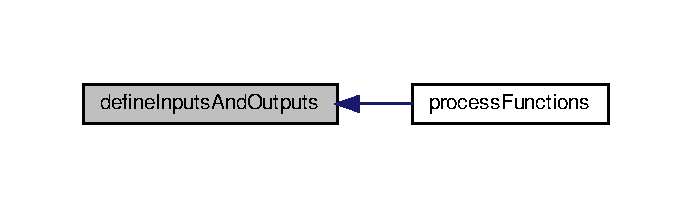
\includegraphics[width=332pt]{namespaceutils_ad890ef664f4412df3dbe4f96f71261bd_icgraph}
\end{center}
\end{figure}
\mbox{\Hypertarget{namespaceutils_a01c8b36149daaab35946bf42cf90fcc1}\label{namespaceutils_a01c8b36149daaab35946bf42cf90fcc1}} 
\index{utils@{utils}!extract\+Function\+Info@{extract\+Function\+Info}}
\index{extract\+Function\+Info@{extract\+Function\+Info}!utils@{utils}}
\subsubsection{\texorpdfstring{extract\+Function\+Info()}{extractFunctionInfo()}}
{\footnotesize\ttfamily def utils.\+extract\+Function\+Info (\begin{DoxyParamCaption}\item[{}]{node,  }\item[{}]{function\+Info }\end{DoxyParamCaption})}

\begin{DoxyVerb}@brief Extracts information about a function, including parameters, local variables, and assignment nodes.

This function collects parameters, local variables, and assignment nodes from a function definition node and
stores the information in the functionInfo dictionary.

@param node: The function definition node to extract information from.
@type node: pycparser.c_ast.FuncDef
@param functionInfo: Dictionary to store extracted function information.
@type functionInfo: dict
\end{DoxyVerb}
 

Definition at line 44 of file utils.\+py.


\begin{DoxyCode}
44 \textcolor{keyword}{def }\hyperlink{namespaceutils_a01c8b36149daaab35946bf42cf90fcc1}{extractFunctionInfo}(node,functionInfo):
45     \textcolor{stringliteral}{"""
}
46 \textcolor{stringliteral}{    @brief Extracts information about a function, including parameters, local variables, and assignment
       nodes.
}
47 \textcolor{stringliteral}{
}
48 \textcolor{stringliteral}{    This function collects parameters, local variables, and assignment nodes from a function definition
       node and
}
49 \textcolor{stringliteral}{    stores the information in the functionInfo dictionary.
}
50 \textcolor{stringliteral}{
}
51 \textcolor{stringliteral}{    @param node: The function definition node to extract information from.
}
52 \textcolor{stringliteral}{    @type node: pycparser.c\_ast.FuncDef
}
53 \textcolor{stringliteral}{    @param functionInfo: Dictionary to store extracted function information.
}
54 \textcolor{stringliteral}{    @type functionInfo: dict
}
55 \textcolor{stringliteral}{    """}
56     function\_name = node.decl.name
57     parameters = []
58     localVariables = []
59     localVariablesType = []
60     assignmentNodes = []
61 
62     \textcolor{keywordflow}{if} node.decl.type.args:
63         \textcolor{keywordflow}{for} param\_decl \textcolor{keywordflow}{in} node.decl.type.args.params:
64             parameters.append(param\_decl.name)
65     
66     functionBody = node.body
67     \textcolor{keywordflow}{for} blockItem \textcolor{keywordflow}{in} functionBody.block\_items:
68         \textcolor{keywordflow}{if} isinstance(blockItem,c\_ast.Decl):
69             typeOfId = \hyperlink{namespaceutils_a63a441384eb62bbf51329ab7e1b212a6}{getType}(blockItem.type.type)
70             localVariablesType.append(typeOfId)
71             localVariables.append(blockItem.name)
72         \textcolor{keywordflow}{if} isinstance(blockItem,c\_ast.Assignment):
73             \textcolor{keywordflow}{if} isinstance(blockItem.lvalue,c\_ast.UnaryOp):
74                 blockItem.lvalue = c\_ast.ID(blockItem.lvalue.expr.name)
75             visitor = LocalVariablesModifier(localVariables,function\_name)
76             visitor.visit(blockItem)
77             assignmentNodes.append(blockItem)
78     
79     \textcolor{keywordflow}{for} index \textcolor{keywordflow}{in} range(len(localVariables)):
80         localVariables[index] += (\textcolor{stringliteral}{'\_'} + function\_name)
81 
82     functionInfo[function\_name] = \{
83         \textcolor{stringliteral}{'parameters'} : parameters,
84         \textcolor{stringliteral}{'localVariables'} : localVariables,
85         \textcolor{stringliteral}{'localVariablesType'} : localVariablesType,
86         \textcolor{stringliteral}{'assignmentNodes'} : assignmentNodes,
87         \textcolor{stringliteral}{'firstTimeProcessing'} : \textcolor{keyword}{True},
88         \textcolor{stringliteral}{'timesCalled'} : 0
89     \}
90 
\end{DoxyCode}
Here is the call graph for this function\+:\nopagebreak
\begin{figure}[H]
\begin{center}
\leavevmode
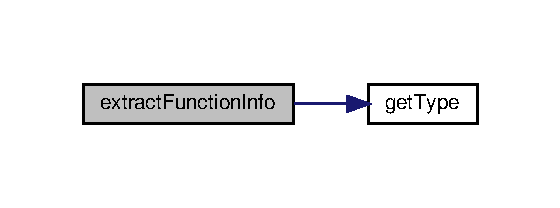
\includegraphics[width=269pt]{namespaceutils_a01c8b36149daaab35946bf42cf90fcc1_cgraph}
\end{center}
\end{figure}
Here is the caller graph for this function\+:\nopagebreak
\begin{figure}[H]
\begin{center}
\leavevmode
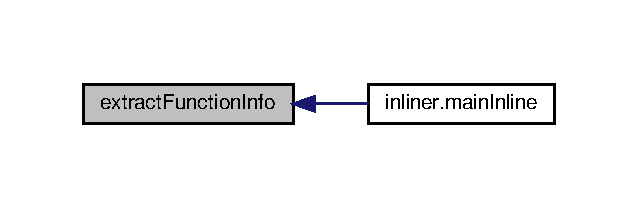
\includegraphics[width=306pt]{namespaceutils_a01c8b36149daaab35946bf42cf90fcc1_icgraph}
\end{center}
\end{figure}
\mbox{\Hypertarget{namespaceutils_a5ab527c9affdfd39949f2e88c4299989}\label{namespaceutils_a5ab527c9affdfd39949f2e88c4299989}} 
\index{utils@{utils}!generate\+\_\+c\+\_\+file@{generate\+\_\+c\+\_\+file}}
\index{generate\+\_\+c\+\_\+file@{generate\+\_\+c\+\_\+file}!utils@{utils}}
\subsubsection{\texorpdfstring{generate\+\_\+c\+\_\+file()}{generate\_c\_file()}}
{\footnotesize\ttfamily def utils.\+generate\+\_\+c\+\_\+file (\begin{DoxyParamCaption}\item[{}]{ast,  }\item[{}]{filename }\end{DoxyParamCaption})}

\begin{DoxyVerb}@brief Generates C code from the provided Abstract Syntax Tree (AST) and writes it to a file.

This function uses the C generator to convert the AST into C code and saves the generated code to the specified file.

@param ast: The Abstract Syntax Tree to be converted into C code.
@type ast: pycparser.c_ast.FileAST
@param filename: The name of the file where the generated C code will be saved.
@type filename: str
\end{DoxyVerb}
 

Definition at line 200 of file utils.\+py.


\begin{DoxyCode}
200 \textcolor{keyword}{def }\hyperlink{namespacePostProcessor_1_1utils_a998fb471074ff747973a0d974eb9fbd1}{generate\_c\_file}(ast,filename):
201     \textcolor{stringliteral}{"""
}
202 \textcolor{stringliteral}{    @brief Generates C code from the provided Abstract Syntax Tree (AST) and writes it to a file.
}
203 \textcolor{stringliteral}{
}
204 \textcolor{stringliteral}{    This function uses the C generator to convert the AST into C code and saves the generated code to the
       specified file.
}
205 \textcolor{stringliteral}{
}
206 \textcolor{stringliteral}{    @param ast: The Abstract Syntax Tree to be converted into C code.
}
207 \textcolor{stringliteral}{    @type ast: pycparser.c\_ast.FileAST
}
208 \textcolor{stringliteral}{    @param filename: The name of the file where the generated C code will be saved.
}
209 \textcolor{stringliteral}{    @type filename: str
}
210 \textcolor{stringliteral}{    """}
211     generator = c\_generator.CGenerator()
212     with open(filename, \textcolor{stringliteral}{'w'}) \textcolor{keyword}{as} output\_file:
213         print(generator.visit(ast), file=output\_file)
\end{DoxyCode}
Here is the caller graph for this function\+:\nopagebreak
\begin{figure}[H]
\begin{center}
\leavevmode
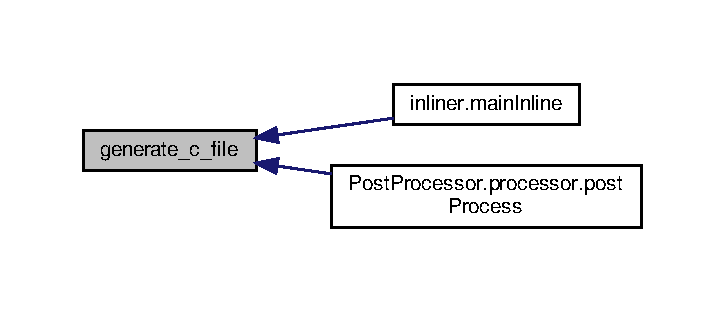
\includegraphics[width=348pt]{namespaceutils_a5ab527c9affdfd39949f2e88c4299989_icgraph}
\end{center}
\end{figure}
\mbox{\Hypertarget{namespaceutils_a04fa4bbfa41595f584571fb61a6047c5}\label{namespaceutils_a04fa4bbfa41595f584571fb61a6047c5}} 
\index{utils@{utils}!get\+Function\+Assignments@{get\+Function\+Assignments}}
\index{get\+Function\+Assignments@{get\+Function\+Assignments}!utils@{utils}}
\subsubsection{\texorpdfstring{get\+Function\+Assignments()}{getFunctionAssignments()}}
{\footnotesize\ttfamily def utils.\+get\+Function\+Assignments (\begin{DoxyParamCaption}\item[{}]{function\+Info,  }\item[{}]{argument\+Map,  }\item[{}]{local\+Variables\+Map,  }\item[{}]{assignment\+Nodes }\end{DoxyParamCaption})}

\begin{DoxyVerb}@brief Extracts and modifies function assignment nodes based on argument and local variable mappings.

This function processes the assignment nodes of a given function, updating identifiers according to the provided 
argument and local variable mappings, and appends the modified nodes to the assignmentNodes list.

@param functionInfo: Dictionary containing function information, including assignment nodes.
@type functionInfo: dict
@param argumentMap: Mapping from function parameters to argument names.
@type argumentMap: dict
@param localVariablesMap: Mapping from local variables to new variable names.
@type localVariablesMap: dict
@param assignmentNodes: List to which modified assignment nodes will be appended.
@type assignmentNodes: list
\end{DoxyVerb}
 

Definition at line 6 of file utils.\+py.


\begin{DoxyCode}
6 \textcolor{keyword}{def }\hyperlink{namespaceutils_a04fa4bbfa41595f584571fb61a6047c5}{getFunctionAssignments}(functionInfo,argumentMap,localVariablesMap,assignmentNodes
      ):
7     \textcolor{stringliteral}{"""
}
8 \textcolor{stringliteral}{    @brief Extracts and modifies function assignment nodes based on argument and local variable mappings.
}
9 \textcolor{stringliteral}{
}
10 \textcolor{stringliteral}{    This function processes the assignment nodes of a given function, updating identifiers according to the
       provided 
}
11 \textcolor{stringliteral}{    argument and local variable mappings, and appends the modified nodes to the assignmentNodes list.
}
12 \textcolor{stringliteral}{
}
13 \textcolor{stringliteral}{    @param functionInfo: Dictionary containing function information, including assignment nodes.
}
14 \textcolor{stringliteral}{    @type functionInfo: dict
}
15 \textcolor{stringliteral}{    @param argumentMap: Mapping from function parameters to argument names.
}
16 \textcolor{stringliteral}{    @type argumentMap: dict
}
17 \textcolor{stringliteral}{    @param localVariablesMap: Mapping from local variables to new variable names.
}
18 \textcolor{stringliteral}{    @type localVariablesMap: dict
}
19 \textcolor{stringliteral}{    @param assignmentNodes: List to which modified assignment nodes will be appended.
}
20 \textcolor{stringliteral}{    @type assignmentNodes: list
}
21 \textcolor{stringliteral}{    """}
22     copyAssignmentNodes = copy.deepcopy(functionInfo[\textcolor{stringliteral}{'assignmentNodes'}])
23     \textcolor{keywordflow}{for} node \textcolor{keywordflow}{in} copyAssignmentNodes:
24         visitor = IdVisitor(argumentMap,localVariablesMap)
25         visitor.visit(node)
26         assignmentNodes.append(node);
27 
\end{DoxyCode}
Here is the caller graph for this function\+:\nopagebreak
\begin{figure}[H]
\begin{center}
\leavevmode
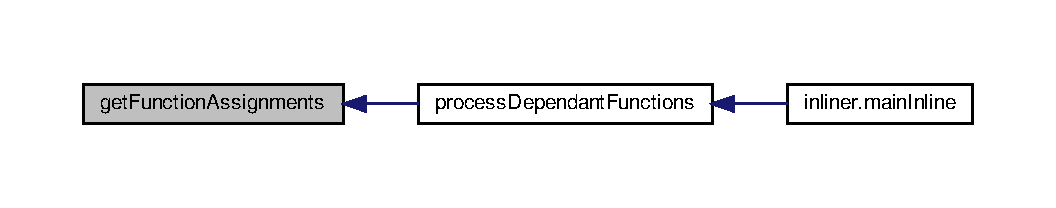
\includegraphics[width=350pt]{namespaceutils_a04fa4bbfa41595f584571fb61a6047c5_icgraph}
\end{center}
\end{figure}
\mbox{\Hypertarget{namespaceutils_a63a441384eb62bbf51329ab7e1b212a6}\label{namespaceutils_a63a441384eb62bbf51329ab7e1b212a6}} 
\index{utils@{utils}!get\+Type@{get\+Type}}
\index{get\+Type@{get\+Type}!utils@{utils}}
\subsubsection{\texorpdfstring{get\+Type()}{getType()}}
{\footnotesize\ttfamily def utils.\+get\+Type (\begin{DoxyParamCaption}\item[{}]{node }\end{DoxyParamCaption})}

\begin{DoxyVerb}@brief Retrieves the type name from a type node.

This function extracts the type name from a given node. It supports both IdentifierType and other type nodes.

@param node: The type node from which to extract the type name.
@type node: pycparser.c_ast.Type
@return: The type name as a string.
@rtype: str
\end{DoxyVerb}
 

Definition at line 28 of file utils.\+py.


\begin{DoxyCode}
28 \textcolor{keyword}{def }\hyperlink{namespaceutils_a63a441384eb62bbf51329ab7e1b212a6}{getType}(node):
29     \textcolor{stringliteral}{"""
}
30 \textcolor{stringliteral}{    @brief Retrieves the type name from a type node.
}
31 \textcolor{stringliteral}{
}
32 \textcolor{stringliteral}{    This function extracts the type name from a given node. It supports both IdentifierType and other type
       nodes.
}
33 \textcolor{stringliteral}{
}
34 \textcolor{stringliteral}{    @param node: The type node from which to extract the type name.
}
35 \textcolor{stringliteral}{    @type node: pycparser.c\_ast.Type
}
36 \textcolor{stringliteral}{    @return: The type name as a string.
}
37 \textcolor{stringliteral}{    @rtype: str
}
38 \textcolor{stringliteral}{    """}
39     \textcolor{keywordflow}{if} isinstance(node,c\_ast.IdentifierType):
40         \textcolor{keywordflow}{return} node.names[0]
41     \textcolor{keywordflow}{else}:
42         \textcolor{keywordflow}{return} node.type.names[0]
43 
\end{DoxyCode}
Here is the caller graph for this function\+:\nopagebreak
\begin{figure}[H]
\begin{center}
\leavevmode
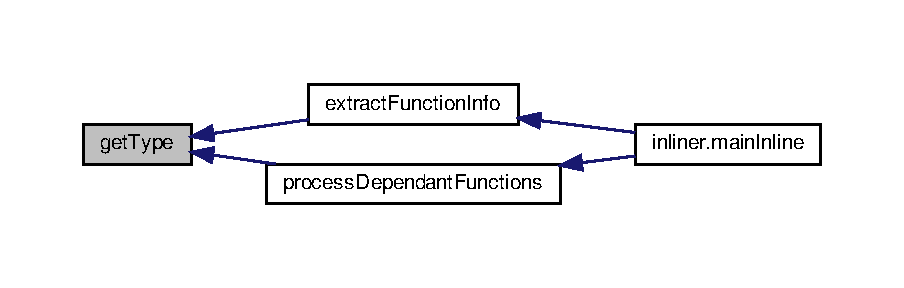
\includegraphics[width=350pt]{namespaceutils_a63a441384eb62bbf51329ab7e1b212a6_icgraph}
\end{center}
\end{figure}
\mbox{\Hypertarget{namespaceutils_a694fa47d55cc41b3f9e86ab2f90e98f3}\label{namespaceutils_a694fa47d55cc41b3f9e86ab2f90e98f3}} 
\index{utils@{utils}!insert\+Assignments\+And\+Decl\+For\+Constants@{insert\+Assignments\+And\+Decl\+For\+Constants}}
\index{insert\+Assignments\+And\+Decl\+For\+Constants@{insert\+Assignments\+And\+Decl\+For\+Constants}!utils@{utils}}
\subsubsection{\texorpdfstring{insert\+Assignments\+And\+Decl\+For\+Constants()}{insertAssignmentsAndDeclForConstants()}}
{\footnotesize\ttfamily def utils.\+insert\+Assignments\+And\+Decl\+For\+Constants (\begin{DoxyParamCaption}\item[{}]{ast,  }\item[{}]{const\+Arr }\end{DoxyParamCaption})}

\begin{DoxyVerb}@brief Inserts assignments and declarations for constants into the AST.

This function adds declarations and assignments for constants into the function's parameter list and body nodes.

@param ast: The Abstract Syntax Tree to be updated.
@type ast: pycparser.c_ast.FileAST
@param constArr: List of constant names to be added to the AST.
@type constArr: list of str
@return: The updated Abstract Syntax Tree.
@rtype: pycparser.c_ast.FileAST
\end{DoxyVerb}
 

Definition at line 176 of file utils.\+py.


\begin{DoxyCode}
176 \textcolor{keyword}{def }\hyperlink{namespaceutils_a694fa47d55cc41b3f9e86ab2f90e98f3}{insertAssignmentsAndDeclForConstants}(ast,constArr):
177     \textcolor{stringliteral}{"""
}
178 \textcolor{stringliteral}{    @brief Inserts assignments and declarations for constants into the AST.
}
179 \textcolor{stringliteral}{
}
180 \textcolor{stringliteral}{    This function adds declarations and assignments for constants into the function's parameter list and
       body nodes.
}
181 \textcolor{stringliteral}{
}
182 \textcolor{stringliteral}{    @param ast: The Abstract Syntax Tree to be updated.
}
183 \textcolor{stringliteral}{    @type ast: pycparser.c\_ast.FileAST
}
184 \textcolor{stringliteral}{    @param constArr: List of constant names to be added to the AST.
}
185 \textcolor{stringliteral}{    @type constArr: list of str
}
186 \textcolor{stringliteral}{    @return: The updated Abstract Syntax Tree.
}
187 \textcolor{stringliteral}{    @rtype: pycparser.c\_ast.FileAST
}
188 \textcolor{stringliteral}{    """}
189     paramList = ast.ext[0].decl.type.args.params
190     bodyNodes = ast.ext[0].body.block\_items
191     \textcolor{keywordflow}{for} const \textcolor{keywordflow}{in} constArr:
192         bodyNodes.insert(0,\hyperlink{namespaceastNodes_a2403f5d006e54f20e614226280cb6cbc}{getSimpleAssignmentNode}(const + \textcolor{stringliteral}{"\_inp"},const))
193     \textcolor{keywordflow}{for} const \textcolor{keywordflow}{in} constArr:
194         bodyNodes.insert(0,\hyperlink{namespaceastNodes_ae5e5c7f09a1586002b20db6d72f6d30b}{getDeclarationNode}(const + \textcolor{stringliteral}{"\_inp"},\textcolor{stringliteral}{"int"}))
195     \textcolor{keywordflow}{for} const \textcolor{keywordflow}{in} constArr:
196         paramList.append(\hyperlink{namespaceastNodes_ae5e5c7f09a1586002b20db6d72f6d30b}{getDeclarationNode}(const,\textcolor{stringliteral}{"int"}))
197     \textcolor{keywordflow}{return} ast
198 
199 
\end{DoxyCode}
Here is the call graph for this function\+:\nopagebreak
\begin{figure}[H]
\begin{center}
\leavevmode
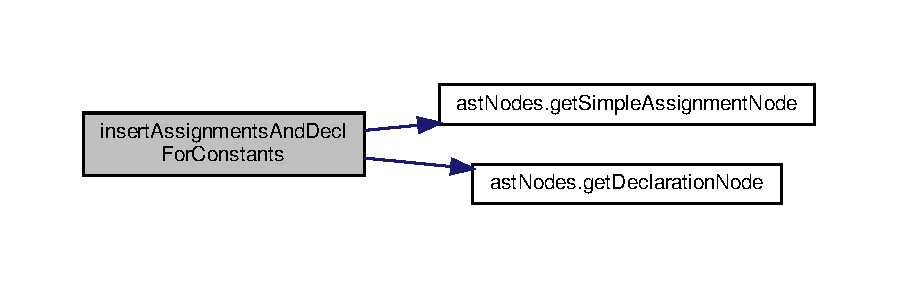
\includegraphics[width=350pt]{namespaceutils_a694fa47d55cc41b3f9e86ab2f90e98f3_cgraph}
\end{center}
\end{figure}
Here is the caller graph for this function\+:\nopagebreak
\begin{figure}[H]
\begin{center}
\leavevmode
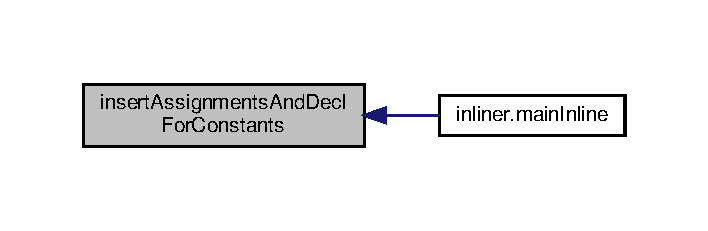
\includegraphics[width=340pt]{namespaceutils_a694fa47d55cc41b3f9e86ab2f90e98f3_icgraph}
\end{center}
\end{figure}
\mbox{\Hypertarget{namespaceutils_aaebca5d3cb4f9c54ab10670ed1ce52a9}\label{namespaceutils_aaebca5d3cb4f9c54ab10670ed1ce52a9}} 
\index{utils@{utils}!merge\+Constants@{merge\+Constants}}
\index{merge\+Constants@{merge\+Constants}!utils@{utils}}
\subsubsection{\texorpdfstring{merge\+Constants()}{mergeConstants()}}
{\footnotesize\ttfamily def utils.\+merge\+Constants (\begin{DoxyParamCaption}\item[{}]{ast }\end{DoxyParamCaption})}

\begin{DoxyVerb}@brief Placeholder function for merging constants.

This function currently does nothing and is intended to be implemented with logic for merging constants in the AST.

@param ast: The Abstract Syntax Tree to be processed.
@type ast: pycparser.c_ast.FileAST
\end{DoxyVerb}
 

Definition at line 165 of file utils.\+py.


\begin{DoxyCode}
165 \textcolor{keyword}{def }\hyperlink{namespaceutils_aaebca5d3cb4f9c54ab10670ed1ce52a9}{mergeConstants}(ast):
166     \textcolor{stringliteral}{"""
}
167 \textcolor{stringliteral}{    @brief Placeholder function for merging constants.
}
168 \textcolor{stringliteral}{
}
169 \textcolor{stringliteral}{    This function currently does nothing and is intended to be implemented with logic for merging constants
       in the AST.
}
170 \textcolor{stringliteral}{
}
171 \textcolor{stringliteral}{    @param ast: The Abstract Syntax Tree to be processed.
}
172 \textcolor{stringliteral}{    @type ast: pycparser.c\_ast.FileAST
}
173 \textcolor{stringliteral}{    """}
174     a = 1
175 
\end{DoxyCode}
\mbox{\Hypertarget{namespaceutils_a6c1d5e886507ec0741fb0fce3f642c5b}\label{namespaceutils_a6c1d5e886507ec0741fb0fce3f642c5b}} 
\index{utils@{utils}!process\+Dependant\+Functions@{process\+Dependant\+Functions}}
\index{process\+Dependant\+Functions@{process\+Dependant\+Functions}!utils@{utils}}
\subsubsection{\texorpdfstring{process\+Dependant\+Functions()}{processDependantFunctions()}}
{\footnotesize\ttfamily def utils.\+process\+Dependant\+Functions (\begin{DoxyParamCaption}\item[{}]{node,  }\item[{}]{function\+Info,  }\item[{}]{is\+Top\+Module }\end{DoxyParamCaption})}

\begin{DoxyVerb}@brief Processes function calls within a given function, handling parameter and local variable modifications.

This function modifies function calls within the function body, updates the parameter and local variable mappings,
and inserts appropriate declarations and assignments into the function body.

@param node: The function definition node to process.
@type node: pycparser.c_ast.FuncDef
@param functionInfo: Dictionary containing information about all functions.
@type functionInfo: dict
@param isTopModule: Boolean indicating if the function is the top module.
@type isTopModule: bool
\end{DoxyVerb}
 

Definition at line 91 of file utils.\+py.


\begin{DoxyCode}
91 \textcolor{keyword}{def }\hyperlink{namespaceutils_a6c1d5e886507ec0741fb0fce3f642c5b}{processDependantFunctions}(node,functionInfo,isTopModule):
92     \textcolor{stringliteral}{"""
}
93 \textcolor{stringliteral}{    @brief Processes function calls within a given function, handling parameter and local variable
       modifications.
}
94 \textcolor{stringliteral}{
}
95 \textcolor{stringliteral}{    This function modifies function calls within the function body, updates the parameter and local
       variable mappings,
}
96 \textcolor{stringliteral}{    and inserts appropriate declarations and assignments into the function body.
}
97 \textcolor{stringliteral}{
}
98 \textcolor{stringliteral}{    @param node: The function definition node to process.
}
99 \textcolor{stringliteral}{    @type node: pycparser.c\_ast.FuncDef
}
100 \textcolor{stringliteral}{    @param functionInfo: Dictionary containing information about all functions.
}
101 \textcolor{stringliteral}{    @type functionInfo: dict
}
102 \textcolor{stringliteral}{    @param isTopModule: Boolean indicating if the function is the top module.
}
103 \textcolor{stringliteral}{    @type isTopModule: bool
}
104 \textcolor{stringliteral}{    """}
105     functionBody = node.body
106     changedInputMap = \{\}
107     bodyNodes = []
108 
109     \textcolor{keywordflow}{if} isTopModule:
110         \textcolor{keywordflow}{if} node.decl.type.args:
111             \textcolor{keywordflow}{for} param\_decl \textcolor{keywordflow}{in} node.decl.type.args.params:
112                 visitor = DeclVisitor()
113                 visitor.visit(param\_decl)
114                 declType = param\_decl.type
115                 \textcolor{keywordflow}{if} isinstance(declType,c\_ast.TypeDecl):
116                     typeOfId = \hyperlink{namespaceutils_a63a441384eb62bbf51329ab7e1b212a6}{getType}(declType.type)
117                     bodyNodes.append(\hyperlink{namespaceastNodes_ae5e5c7f09a1586002b20db6d72f6d30b}{getDeclarationNode}(param\_decl.name + \textcolor{stringliteral}{'\_inp'},typeOfId
      ))
118                     changedInputMap[param\_decl.name] = param\_decl.name + \textcolor{stringliteral}{'\_inp'}
119             \textcolor{keywordflow}{for} param\_decl \textcolor{keywordflow}{in} node.decl.type.args.params:
120                 declType = param\_decl.type
121                 \textcolor{keywordflow}{if} isinstance(declType,c\_ast.TypeDecl):
122                     bodyNodes.append(\hyperlink{namespaceastNodes_a2403f5d006e54f20e614226280cb6cbc}{getSimpleAssignmentNode}(param\_decl.name + \textcolor{stringliteral}{'\_inp
      '},param\_decl.name))
123     
124     \textcolor{keywordflow}{for} blockItem \textcolor{keywordflow}{in} functionBody.block\_items:
125         \textcolor{keywordflow}{if} isinstance(blockItem,c\_ast.Decl):
126             visitor = DeclVisitor()
127             visitor.visit(blockItem)
128             bodyNodes.append(blockItem)
129         
130         \textcolor{keywordflow}{if} isinstance(blockItem,c\_ast.Assignment):
131             visitor = InputParamModifier(changedInputMap)
132             visitor.visit(blockItem)
133             bodyNodes.append(blockItem)
134 
135         \textcolor{keywordflow}{if} isinstance(blockItem,c\_ast.FuncCall):
136             argumentMap = \{\}
137             localVariablesMap = \{\}
138             
139             functionName = blockItem.name.name
140             parameters = functionInfo[functionName][\textcolor{stringliteral}{'parameters'}]
141             localVariables = functionInfo[functionName][\textcolor{stringliteral}{'localVariables'}]
142             localVariablesType = functionInfo[functionName][\textcolor{stringliteral}{'localVariablesType'}]
143             timesCalled = functionInfo[functionName][\textcolor{stringliteral}{'timesCalled'}]
144             arguments = blockItem.args.exprs
145             \textcolor{keywordflow}{for} index \textcolor{keywordflow}{in} range(len(arguments)):
146                 \textcolor{keywordflow}{if} isinstance(arguments[index],c\_ast.UnaryOp):
147                     arguments[index] = c\_ast.ID(arguments[index].expr.name)
148 
149             \textcolor{keywordflow}{for} localVariable,localVariableType \textcolor{keywordflow}{in} zip(localVariables,localVariablesType):
150                 declNode = \hyperlink{namespaceastNodes_ae5e5c7f09a1586002b20db6d72f6d30b}{getDeclarationNode}(localVariable + str(timesCalled),
      localVariableType)
151                 localVariablesMap[localVariable] = localVariable + str(timesCalled)
152                 bodyNodes.append(declNode)
153             
154             \textcolor{keywordflow}{for} index \textcolor{keywordflow}{in} range(len(parameters)):
155                 \textcolor{keywordflow}{if} arguments[index].name \textcolor{keywordflow}{in} changedInputMap:
156                     argName = arguments[index].name + \textcolor{stringliteral}{'\_inp'}
157                 \textcolor{keywordflow}{else}:
158                     argName = arguments[index].name
159                 argumentMap[parameters[index]] = argName
160             
161             \hyperlink{namespaceutils_a04fa4bbfa41595f584571fb61a6047c5}{getFunctionAssignments}(functionInfo[functionName],argumentMap,
      localVariablesMap,bodyNodes)
162             functionInfo[functionName][\textcolor{stringliteral}{'timesCalled'}] += 1
163     node.body = c\_ast.Compound(block\_items=bodyNodes)
164 
\end{DoxyCode}
Here is the call graph for this function\+:\nopagebreak
\begin{figure}[H]
\begin{center}
\leavevmode
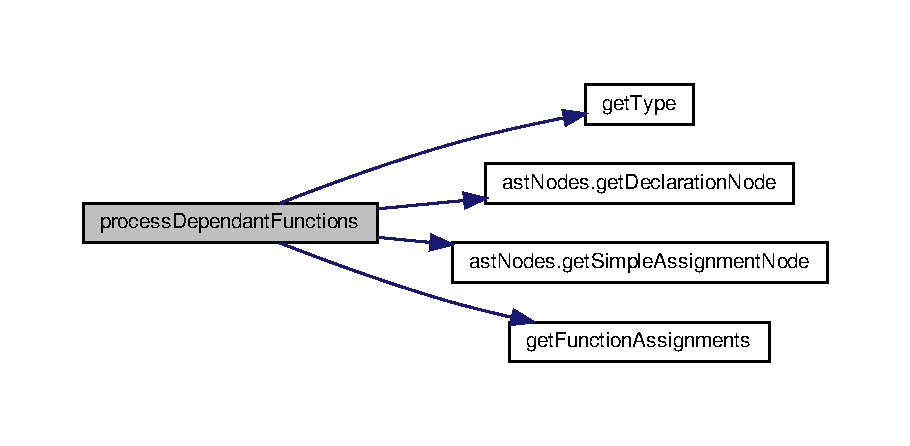
\includegraphics[width=350pt]{namespaceutils_a6c1d5e886507ec0741fb0fce3f642c5b_cgraph}
\end{center}
\end{figure}
Here is the caller graph for this function\+:\nopagebreak
\begin{figure}[H]
\begin{center}
\leavevmode
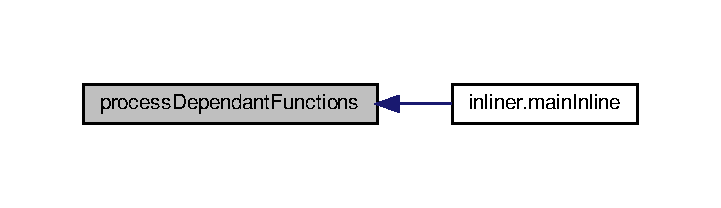
\includegraphics[width=346pt]{namespaceutils_a6c1d5e886507ec0741fb0fce3f642c5b_icgraph}
\end{center}
\end{figure}
\mbox{\Hypertarget{namespaceutils_a4934e690de4b9b81cb16a1df0dbd73b9}\label{namespaceutils_a4934e690de4b9b81cb16a1df0dbd73b9}} 
\index{utils@{utils}!process\+Functions@{process\+Functions}}
\index{process\+Functions@{process\+Functions}!utils@{utils}}
\subsubsection{\texorpdfstring{process\+Functions()}{processFunctions()}}
{\footnotesize\ttfamily def utils.\+process\+Functions (\begin{DoxyParamCaption}\item[{}]{functions,  }\item[{}]{f\+Def,  }\item[{}]{function\+Calls,  }\item[{}]{intermediate\+Assignments }\end{DoxyParamCaption})}

\begin{DoxyVerb}@brief Processes a function definition to extract its inputs, outputs, intermediate variables, and function calls.

This function analyzes the function definition to build a dictionary of function information, including
the inputs, outputs, and function calls. It also updates intermediate variable assignments based on the function body.

@param functions: A dictionary to store information about functions, including their inputs, outputs, and parameter order.
@param fDef: The function definition node from the C Abstract Syntax Tree (AST).
@param functionCalls: A dictionary to store function calls made within the function.
@param intermediateAssignments: A dictionary to store intermediate variable assignments for the function.

@raises ValueError: If the return type of the function is other than `void`.
\end{DoxyVerb}
 

Definition at line 87 of file utils.\+py.


\begin{DoxyCode}
87 \textcolor{keyword}{def }\hyperlink{namespaceutils_a4934e690de4b9b81cb16a1df0dbd73b9}{processFunctions}(functions,fDef,functionCalls,intermediateAssignments):
88     \textcolor{stringliteral}{"""
}
89 \textcolor{stringliteral}{    @brief Processes a function definition to extract its inputs, outputs, intermediate variables, and
       function calls.
}
90 \textcolor{stringliteral}{
}
91 \textcolor{stringliteral}{    This function analyzes the function definition to build a dictionary of function information,
       including
}
92 \textcolor{stringliteral}{    the inputs, outputs, and function calls. It also updates intermediate variable assignments based on the
       function body.
}
93 \textcolor{stringliteral}{
}
94 \textcolor{stringliteral}{    @param functions: A dictionary to store information about functions, including their inputs, outputs,
       and parameter order.
}
95 \textcolor{stringliteral}{    @param fDef: The function definition node from the C Abstract Syntax Tree (AST).
}
96 \textcolor{stringliteral}{    @param functionCalls: A dictionary to store function calls made within the function.
}
97 \textcolor{stringliteral}{    @param intermediateAssignments: A dictionary to store intermediate variable assignments for the
       function.
}
98 \textcolor{stringliteral}{
}
99 \textcolor{stringliteral}{    @raises ValueError: If the return type of the function is other than `void`.
}
100 \textcolor{stringliteral}{    """}
101     regPresent = \textcolor{keyword}{False}
102     function\_decl = fDef.decl
103     fName = function\_decl.name
104     functions[fName] = \{
105         \textcolor{stringliteral}{"inputs"} : [],
106         \textcolor{stringliteral}{"outputs"} : [],
107         \textcolor{stringliteral}{"paramOrder"} : [],
108         \textcolor{stringliteral}{"called"} : 0,
109         \textcolor{stringliteral}{"regPresent"} : \textcolor{keyword}{False}
110     \}
111     functionCalls[fName] = []
112     intermediateAssignments[fName] = \{\}
113 
114     \hyperlink{namespaceutils_ad890ef664f4412df3dbe4f96f71261bd}{defineInputsAndOutputs}(fName,functions,function\_decl)
115 
116     \textcolor{comment}{#type, value
}
117     internalVariables = \{\}
118     exp = \textcolor{stringliteral}{""}
119     function\_body = fDef.body
120     \textcolor{keywordflow}{for} node \textcolor{keywordflow}{in} function\_body.block\_items:
121         \textcolor{keywordflow}{if} isinstance(node,c\_ast.Decl) \textcolor{keywordflow}{and} node.init \textcolor{keywordflow}{is} \textcolor{keywordflow}{not} \textcolor{keywordtype}{None}:
122             regPresent = \hyperlink{namespaceblockHandlers_ad92852be9f2eee24eb76b2dd747e7584}{handleDeclBlock}(node,internalVariables)
123 
124         \textcolor{keywordflow}{elif} isinstance(node,c\_ast.Assignment):
125             regPresent = \hyperlink{namespaceblockHandlers_ac54cbd08eb8b12eed0c801fa775911dd}{handleAssignmentBlock}(node,internalVariables)
126 
127         \textcolor{keywordflow}{elif} isinstance(node,c\_ast.Return):
128             \hyperlink{namespaceblockHandlers_a9a619208834c3d0aa0861354376f5208}{handleReturnBlock}(node,internalVariables,functions,fName)
129 
130         \textcolor{keywordflow}{elif} isinstance(node,c\_ast.FuncCall):
131             \hyperlink{namespaceblockHandlers_ac034bd474478ead202ae756242b4348c}{handleFuncCallBlock}(node,functions,fName,functionCalls,internalVariables)
132 
133         if(regPresent):
134             functions[fName][\textcolor{stringliteral}{"regPresent"}] = regPresent
135     intermediateAssignments[fName] = internalVariables
136     
\end{DoxyCode}
Here is the call graph for this function\+:\nopagebreak
\begin{figure}[H]
\begin{center}
\leavevmode
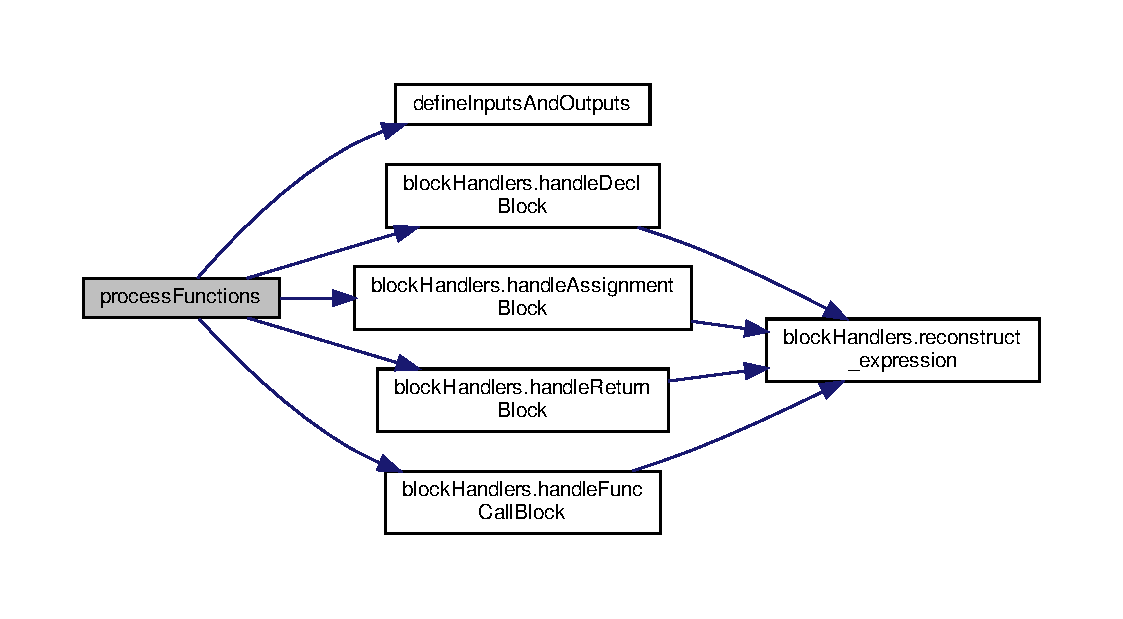
\includegraphics[width=350pt]{namespaceutils_a4934e690de4b9b81cb16a1df0dbd73b9_cgraph}
\end{center}
\end{figure}
\mbox{\Hypertarget{namespaceutils_a6f07e72ab5f460900eea8da9ad34aeec}\label{namespaceutils_a6f07e72ab5f460900eea8da9ad34aeec}} 
\index{utils@{utils}!write\+Verilog\+To\+File@{write\+Verilog\+To\+File}}
\index{write\+Verilog\+To\+File@{write\+Verilog\+To\+File}!utils@{utils}}
\subsubsection{\texorpdfstring{write\+Verilog\+To\+File()}{writeVerilogToFile()}}
{\footnotesize\ttfamily def utils.\+write\+Verilog\+To\+File (\begin{DoxyParamCaption}\item[{}]{func\+Name,  }\item[{}]{functions,  }\item[{}]{internal\+Variables,  }\item[{}]{function\+Calls,  }\item[{}]{filename,  }\item[{}]{width }\end{DoxyParamCaption})}

\begin{DoxyVerb}@brief Writes the Verilog code for a given function to a file.

This function generates a Verilog module for the specified function based on its inputs, outputs,
intermediate variables, and function calls. It writes the module declaration, input and output ports,
intermediate value declarations, wire and reg assignments, and instantiations of other modules.

@param funcName: The name of the function for which the Verilog code is generated.
@param functions: A dictionary containing information about functions, including their inputs, outputs, and parameter order.
@param internalVariables: A dictionary of internal variables used in the function, including their types and values.
@param functionCalls: A dictionary of function calls made within the function, including the instance names and parameter lists.
@param filename: The name of the file to which the Verilog code will be written.
@param width: The bit width for the variables. If '0', no width is added; otherwise, a range is added to the variable declaration.

@raises IOError: If the file cannot be opened or written to.
\end{DoxyVerb}
 

Definition at line 5 of file utils.\+py.


\begin{DoxyCode}
5 \textcolor{keyword}{def }\hyperlink{namespaceutils_a6f07e72ab5f460900eea8da9ad34aeec}{writeVerilogToFile}(funcName, functions, internalVariables, functionCalls, 
      filename,width):
6     \textcolor{comment}{#width = " [7:0] " if width=='int' else " "
}
7     \textcolor{stringliteral}{"""
}
8 \textcolor{stringliteral}{    @brief Writes the Verilog code for a given function to a file.
}
9 \textcolor{stringliteral}{
}
10 \textcolor{stringliteral}{    This function generates a Verilog module for the specified function based on its inputs, outputs,
}
11 \textcolor{stringliteral}{    intermediate variables, and function calls. It writes the module declaration, input and output ports,
}
12 \textcolor{stringliteral}{    intermediate value declarations, wire and reg assignments, and instantiations of other modules.
}
13 \textcolor{stringliteral}{
}
14 \textcolor{stringliteral}{    @param funcName: The name of the function for which the Verilog code is generated.
}
15 \textcolor{stringliteral}{    @param functions: A dictionary containing information about functions, including their inputs, outputs,
       and parameter order.
}
16 \textcolor{stringliteral}{    @param internalVariables: A dictionary of internal variables used in the function, including their
       types and values.
}
17 \textcolor{stringliteral}{    @param functionCalls: A dictionary of function calls made within the function, including the instance
       names and parameter lists.
}
18 \textcolor{stringliteral}{    @param filename: The name of the file to which the Verilog code will be written.
}
19 \textcolor{stringliteral}{    @param width: The bit width for the variables. If '0', no width is added; otherwise, a range is added
       to the variable declaration.
}
20 \textcolor{stringliteral}{
}
21 \textcolor{stringliteral}{    @raises IOError: If the file cannot be opened or written to.
}
22 \textcolor{stringliteral}{    """}
23     width = \textcolor{stringliteral}{" "} \textcolor{keywordflow}{if} width==\textcolor{stringliteral}{'0'} \textcolor{keywordflow}{else} \textcolor{stringliteral}{" ["} + width + \textcolor{stringliteral}{":0] "}
24     with open(filename, \textcolor{stringliteral}{'w'}) \textcolor{keyword}{as} file:
25         \textcolor{comment}{# Redirect print output to the file
}
26         print(\textcolor{stringliteral}{"module "} + funcName + \textcolor{stringliteral}{"("}, file=file)
27         \textcolor{keywordflow}{for} ip \textcolor{keywordflow}{in} functions[funcName][\textcolor{stringliteral}{"inputs"}]:
28             print(\textcolor{stringliteral}{"    "} + ip + \textcolor{stringliteral}{","}, file=file)
29         \textcolor{keywordflow}{for} op \textcolor{keywordflow}{in} functions[funcName][\textcolor{stringliteral}{"outputs"}]:
30             print(\textcolor{stringliteral}{"    "} + op + \textcolor{stringliteral}{","}, file=file)
31         print(\textcolor{stringliteral}{");"}, file=file)
32 
33         print(\textcolor{stringliteral}{"//INPUTS"}, file=file)
34         \textcolor{keywordflow}{for} ip \textcolor{keywordflow}{in} functions[funcName][\textcolor{stringliteral}{"inputs"}]:
35             \textcolor{keywordflow}{if} (ip==\textcolor{stringliteral}{"clk"}):
36                 print(\textcolor{stringliteral}{"    input "} +ip + \textcolor{stringliteral}{";"}, file=file)
37             \textcolor{keywordflow}{else}:
38                 print(\textcolor{stringliteral}{"    input "} + width +ip + \textcolor{stringliteral}{";"}, file=file)
39 
40         print(\textcolor{stringliteral}{"//OUTPUTS"}, file=file)
41         \textcolor{keywordflow}{for} op \textcolor{keywordflow}{in} functions[funcName][\textcolor{stringliteral}{"outputs"}]:
42             \textcolor{keywordflow}{if} internalVariables[op][\textcolor{stringliteral}{"type"}] == \textcolor{stringliteral}{"reg"}:
43                 print(\textcolor{stringliteral}{"    output reg "} + width + op + \textcolor{stringliteral}{";"}, file=file)
44             \textcolor{keywordflow}{else}:
45                 print(\textcolor{stringliteral}{"    output "} + width + op + \textcolor{stringliteral}{";"}, file=file)
46 
47         \textcolor{comment}{# intermediate value decl
}
48         print(\textcolor{stringliteral}{"//Intermediate values"}, file=file)
49         \textcolor{keywordflow}{for} key \textcolor{keywordflow}{in} internalVariables.keys():
50             \textcolor{keywordflow}{if} key \textcolor{keywordflow}{not} \textcolor{keywordflow}{in} functions[funcName][\textcolor{stringliteral}{"outputs"}]:
51                 print(\textcolor{stringliteral}{"    "} + internalVariables[key][\textcolor{stringliteral}{"type"}] + width + key + \textcolor{stringliteral}{";"}, file=file)
52 
53         \textcolor{comment}{# wire assignments
}
54         print(\textcolor{stringliteral}{""}, file=file)
55         \textcolor{keywordflow}{for} key \textcolor{keywordflow}{in} internalVariables.keys():
56             \textcolor{keywordflow}{if} internalVariables[key][\textcolor{stringliteral}{"type"}] == \textcolor{stringliteral}{"wire"}:
57                 print(\textcolor{stringliteral}{"    assign "} + key + \textcolor{stringliteral}{" = "} + internalVariables[key][\textcolor{stringliteral}{"value"}] + \textcolor{stringliteral}{";"}, file=file)
58 
59         \textcolor{comment}{# reg assignments
}
60         print(\textcolor{stringliteral}{""}, file=file)
61         \textcolor{keywordflow}{if} functions[funcName][\textcolor{stringliteral}{"regPresent"}] \textcolor{keywordflow}{is} \textcolor{keyword}{True}:
62             print(\textcolor{stringliteral}{"    always @(posedge clk) begin"}, file=file)
63             \textcolor{keywordflow}{for} key \textcolor{keywordflow}{in} internalVariables.keys():
64                 \textcolor{keywordflow}{if} internalVariables[key][\textcolor{stringliteral}{"type"}] == \textcolor{stringliteral}{"reg"}:
65                     print(\textcolor{stringliteral}{"        "} + key + \textcolor{stringliteral}{" <= "} + internalVariables[key][\textcolor{stringliteral}{"value"}] + \textcolor{stringliteral}{";"}, file=file)
66             print(\textcolor{stringliteral}{"    end"}, file=file)
67 
68         \textcolor{comment}{# module instantiations
}
69         print(\textcolor{stringliteral}{""}, file=file)
70         \textcolor{keywordflow}{for} func\_calls \textcolor{keywordflow}{in} functionCalls[funcName]:
71             callee = func\_calls[\textcolor{stringliteral}{"callee"}]
72             inst = func\_calls[\textcolor{stringliteral}{"instanceName"}]
73             paramList = func\_calls[\textcolor{stringliteral}{"paramList"}]
74             print(\textcolor{stringliteral}{"    "} + callee + \textcolor{stringliteral}{" "} + inst + \textcolor{stringliteral}{"("}, end=\textcolor{stringliteral}{""}, file=file)
75             paramOrder = functions[callee][\textcolor{stringliteral}{"paramOrder"}]
76             \textcolor{keywordflow}{for} i \textcolor{keywordflow}{in} range(len(paramOrder)):
77                 print(\textcolor{stringliteral}{"."} + paramOrder[i] + \textcolor{stringliteral}{"("} + paramList[i] + \textcolor{stringliteral}{")"}, end=\textcolor{stringliteral}{""}, file=file)
78                 \textcolor{keywordflow}{if} i != len(paramOrder) - 1:
79                     print(\textcolor{stringliteral}{", "}, end=\textcolor{stringliteral}{""}, file=file)
80                 \textcolor{keywordflow}{else}:
81                     print(\textcolor{stringliteral}{");"}, file=file)
82 
83         print(\textcolor{stringliteral}{"endmodule"}, file=file)
84         print(\textcolor{stringliteral}{""},file=file)
85 
86 
\end{DoxyCode}

\hypertarget{namespaceVisitors}{}\section{Visitors Namespace Reference}
\label{namespaceVisitors}\index{Visitors@{Visitors}}
\subsection*{Classes}
\begin{DoxyCompactItemize}
\item 
class \hyperlink{classVisitors_1_1ArrayValueReplacer}{Array\+Value\+Replacer}
\item 
class \hyperlink{classVisitors_1_1AssignmentChecker}{Assignment\+Checker}
\item 
class \hyperlink{classVisitors_1_1ConstantMerger}{Constant\+Merger}
\item 
class \hyperlink{classVisitors_1_1ConstToVar}{Const\+To\+Var}
\item 
class \hyperlink{classVisitors_1_1DeclVisitor}{Decl\+Visitor}
\item 
class \hyperlink{classVisitors_1_1FunctionVisitor}{Function\+Visitor}
\item 
class \hyperlink{classVisitors_1_1IdVisitor}{Id\+Visitor}
\item 
class \hyperlink{classVisitors_1_1InputParamModifier}{Input\+Param\+Modifier}
\item 
class \hyperlink{classVisitors_1_1LocalVariablesModifier}{Local\+Variables\+Modifier}
\end{DoxyCompactItemize}

\chapter{Class Documentation}
\hypertarget{classVisitors_1_1ArrayValueReplacer}{}\section{Array\+Value\+Replacer Class Reference}
\label{classVisitors_1_1ArrayValueReplacer}\index{Array\+Value\+Replacer@{Array\+Value\+Replacer}}


Inheritance diagram for Array\+Value\+Replacer\+:\nopagebreak
\begin{figure}[H]
\begin{center}
\leavevmode
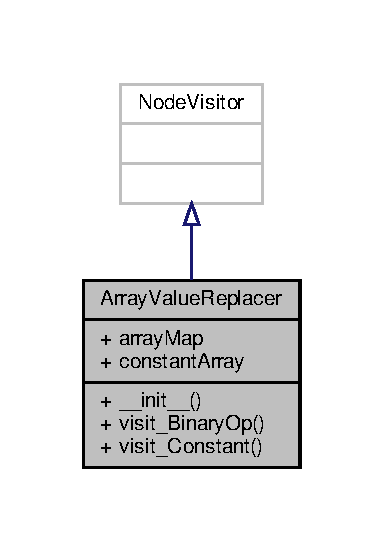
\includegraphics[width=184pt]{classVisitors_1_1ArrayValueReplacer__inherit__graph}
\end{center}
\end{figure}


Collaboration diagram for Array\+Value\+Replacer\+:\nopagebreak
\begin{figure}[H]
\begin{center}
\leavevmode
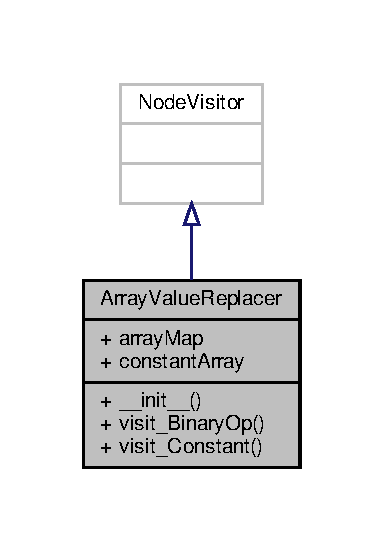
\includegraphics[width=184pt]{classVisitors_1_1ArrayValueReplacer__coll__graph}
\end{center}
\end{figure}
\subsection*{Public Member Functions}
\begin{DoxyCompactItemize}
\item 
def \hyperlink{classVisitors_1_1ArrayValueReplacer_a5f91e1838a4820870ae39478f6195cdc}{\+\_\+\+\_\+init\+\_\+\+\_\+} (self, \hyperlink{classVisitors_1_1ArrayValueReplacer_a3c14dac355802b0266a75f0ee417c14b}{array\+Map}, \hyperlink{classVisitors_1_1ArrayValueReplacer_af8146ce56c53debb8b28c2c19e357077}{constant\+Array})
\item 
def \hyperlink{classVisitors_1_1ArrayValueReplacer_a6329fbf13e2d22de5384fbca843113b8}{visit\+\_\+\+Binary\+Op} (self, node)
\item 
def \hyperlink{classVisitors_1_1ArrayValueReplacer_af527c76a7bf39f449d92deb30bf74144}{visit\+\_\+\+Constant} (self, node)
\end{DoxyCompactItemize}
\subsection*{Public Attributes}
\begin{DoxyCompactItemize}
\item 
\hyperlink{classVisitors_1_1ArrayValueReplacer_a3c14dac355802b0266a75f0ee417c14b}{array\+Map}
\item 
\hyperlink{classVisitors_1_1ArrayValueReplacer_af8146ce56c53debb8b28c2c19e357077}{constant\+Array}
\end{DoxyCompactItemize}


\subsection{Detailed Description}
\begin{DoxyVerb}@brief Replaces array references with their actual values.

This visitor converts array references in expressions to their constant values.

@param arrayMap: Dictionary mapping array names to their values.
@type arrayMap: dict
@param constantArray: List to store unique constants found during replacement.
@type constantArray: list of str
\end{DoxyVerb}
 

Definition at line 152 of file Visitors.\+py.



\subsection{Constructor \& Destructor Documentation}
\mbox{\Hypertarget{classVisitors_1_1ArrayValueReplacer_a5f91e1838a4820870ae39478f6195cdc}\label{classVisitors_1_1ArrayValueReplacer_a5f91e1838a4820870ae39478f6195cdc}} 
\index{Visitors\+::\+Array\+Value\+Replacer@{Visitors\+::\+Array\+Value\+Replacer}!\+\_\+\+\_\+init\+\_\+\+\_\+@{\+\_\+\+\_\+init\+\_\+\+\_\+}}
\index{\+\_\+\+\_\+init\+\_\+\+\_\+@{\+\_\+\+\_\+init\+\_\+\+\_\+}!Visitors\+::\+Array\+Value\+Replacer@{Visitors\+::\+Array\+Value\+Replacer}}
\subsubsection{\texorpdfstring{\+\_\+\+\_\+init\+\_\+\+\_\+()}{\_\_init\_\_()}}
{\footnotesize\ttfamily def \+\_\+\+\_\+init\+\_\+\+\_\+ (\begin{DoxyParamCaption}\item[{}]{self,  }\item[{}]{array\+Map,  }\item[{}]{constant\+Array }\end{DoxyParamCaption})}



Definition at line 163 of file Visitors.\+py.


\begin{DoxyCode}
163     \textcolor{keyword}{def }\_\_init\_\_(self,arrayMap,constantArray):
164         self.arrayMap = arrayMap
165         self.constantArray = constantArray
166 
\end{DoxyCode}


\subsection{Member Function Documentation}
\mbox{\Hypertarget{classVisitors_1_1ArrayValueReplacer_a6329fbf13e2d22de5384fbca843113b8}\label{classVisitors_1_1ArrayValueReplacer_a6329fbf13e2d22de5384fbca843113b8}} 
\index{Visitors\+::\+Array\+Value\+Replacer@{Visitors\+::\+Array\+Value\+Replacer}!visit\+\_\+\+Binary\+Op@{visit\+\_\+\+Binary\+Op}}
\index{visit\+\_\+\+Binary\+Op@{visit\+\_\+\+Binary\+Op}!Visitors\+::\+Array\+Value\+Replacer@{Visitors\+::\+Array\+Value\+Replacer}}
\subsubsection{\texorpdfstring{visit\+\_\+\+Binary\+Op()}{visit\_BinaryOp()}}
{\footnotesize\ttfamily def visit\+\_\+\+Binary\+Op (\begin{DoxyParamCaption}\item[{}]{self,  }\item[{}]{node }\end{DoxyParamCaption})}

\begin{DoxyVerb}@brief Replaces array references in binary operations with their constant values.

@param node: The binary operation node containing the array reference.
@type node: pycparser.c_ast.BinaryOp
\end{DoxyVerb}
 

Definition at line 167 of file Visitors.\+py.


\begin{DoxyCode}
167     \textcolor{keyword}{def }visit\_BinaryOp(self,node):
168         \textcolor{stringliteral}{"""
}
169 \textcolor{stringliteral}{        @brief Replaces array references in binary operations with their constant values.
}
170 \textcolor{stringliteral}{
}
171 \textcolor{stringliteral}{        @param node: The binary operation node containing the array reference.
}
172 \textcolor{stringliteral}{        @type node: pycparser.c\_ast.BinaryOp
}
173 \textcolor{stringliteral}{        """}
174         \textcolor{keywordflow}{if} isinstance(node.right,c\_ast.ArrayRef):
175             arrName = node.right.name.name
176             contents = self.arrayMap[arrName]
177             value = contents[int(node.right.subscript.value)]
178             node.right = c\_ast.Constant(type=\textcolor{stringliteral}{'int'},value=str(value))
179         self.generic\_visit(node)
180     
\end{DoxyCode}
\mbox{\Hypertarget{classVisitors_1_1ArrayValueReplacer_af527c76a7bf39f449d92deb30bf74144}\label{classVisitors_1_1ArrayValueReplacer_af527c76a7bf39f449d92deb30bf74144}} 
\index{Visitors\+::\+Array\+Value\+Replacer@{Visitors\+::\+Array\+Value\+Replacer}!visit\+\_\+\+Constant@{visit\+\_\+\+Constant}}
\index{visit\+\_\+\+Constant@{visit\+\_\+\+Constant}!Visitors\+::\+Array\+Value\+Replacer@{Visitors\+::\+Array\+Value\+Replacer}}
\subsubsection{\texorpdfstring{visit\+\_\+\+Constant()}{visit\_Constant()}}
{\footnotesize\ttfamily def visit\+\_\+\+Constant (\begin{DoxyParamCaption}\item[{}]{self,  }\item[{}]{node }\end{DoxyParamCaption})}

\begin{DoxyVerb}@brief Converts constant values to decimal and stores unique constants.

@param node: The constant node being processed.
@type node: pycparser.c_ast.Constant
\end{DoxyVerb}
 

Definition at line 181 of file Visitors.\+py.


\begin{DoxyCode}
181     \textcolor{keyword}{def }visit\_Constant(self,node):
182         \textcolor{stringliteral}{"""
}
183 \textcolor{stringliteral}{        @brief Converts constant values to decimal and stores unique constants.
}
184 \textcolor{stringliteral}{
}
185 \textcolor{stringliteral}{        @param node: The constant node being processed.
}
186 \textcolor{stringliteral}{        @type node: pycparser.c\_ast.Constant
}
187 \textcolor{stringliteral}{        """}
188         value = node.value
189         \textcolor{keywordflow}{if} value.startswith(\textcolor{stringliteral}{"0x"}):
190             decVal = str(int(value[2:],16))
191         \textcolor{keywordflow}{else}:
192             decVal = value
193         node.value = decVal
194         const = \textcolor{stringliteral}{"dec\_"} + decVal
195         \textcolor{keywordflow}{if} const \textcolor{keywordflow}{not} \textcolor{keywordflow}{in} self.constantArray:
196             self.constantArray.append(\textcolor{stringliteral}{"dec\_"} + decVal)
197 
\end{DoxyCode}


\subsection{Member Data Documentation}
\mbox{\Hypertarget{classVisitors_1_1ArrayValueReplacer_a3c14dac355802b0266a75f0ee417c14b}\label{classVisitors_1_1ArrayValueReplacer_a3c14dac355802b0266a75f0ee417c14b}} 
\index{Visitors\+::\+Array\+Value\+Replacer@{Visitors\+::\+Array\+Value\+Replacer}!array\+Map@{array\+Map}}
\index{array\+Map@{array\+Map}!Visitors\+::\+Array\+Value\+Replacer@{Visitors\+::\+Array\+Value\+Replacer}}
\subsubsection{\texorpdfstring{array\+Map}{arrayMap}}
{\footnotesize\ttfamily array\+Map}



Definition at line 164 of file Visitors.\+py.

\mbox{\Hypertarget{classVisitors_1_1ArrayValueReplacer_af8146ce56c53debb8b28c2c19e357077}\label{classVisitors_1_1ArrayValueReplacer_af8146ce56c53debb8b28c2c19e357077}} 
\index{Visitors\+::\+Array\+Value\+Replacer@{Visitors\+::\+Array\+Value\+Replacer}!constant\+Array@{constant\+Array}}
\index{constant\+Array@{constant\+Array}!Visitors\+::\+Array\+Value\+Replacer@{Visitors\+::\+Array\+Value\+Replacer}}
\subsubsection{\texorpdfstring{constant\+Array}{constantArray}}
{\footnotesize\ttfamily constant\+Array}



Definition at line 165 of file Visitors.\+py.



The documentation for this class was generated from the following file\+:\begin{DoxyCompactItemize}
\item 
Inliner/\hyperlink{Visitors_8py}{Visitors.\+py}\end{DoxyCompactItemize}

\hypertarget{classVisitors_1_1AssignmentChecker}{}\section{Assignment\+Checker Class Reference}
\label{classVisitors_1_1AssignmentChecker}\index{Assignment\+Checker@{Assignment\+Checker}}


Inheritance diagram for Assignment\+Checker\+:\nopagebreak
\begin{figure}[H]
\begin{center}
\leavevmode
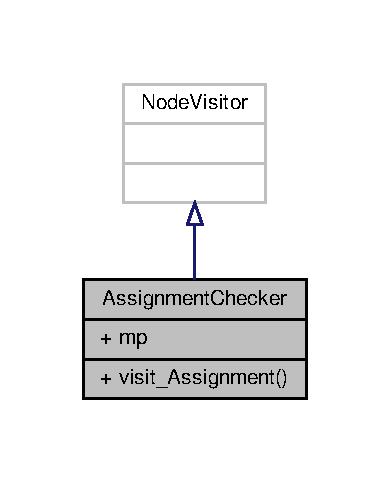
\includegraphics[width=187pt]{classVisitors_1_1AssignmentChecker__inherit__graph}
\end{center}
\end{figure}


Collaboration diagram for Assignment\+Checker\+:\nopagebreak
\begin{figure}[H]
\begin{center}
\leavevmode
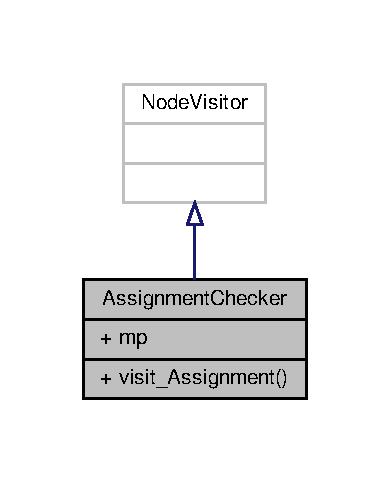
\includegraphics[width=187pt]{classVisitors_1_1AssignmentChecker__coll__graph}
\end{center}
\end{figure}
\subsection*{Public Member Functions}
\begin{DoxyCompactItemize}
\item 
def \hyperlink{classVisitors_1_1AssignmentChecker_adae6ad6f5b94c4acd95924bb3df9ebc8}{visit\+\_\+\+Assignment} (self, node)
\end{DoxyCompactItemize}
\subsection*{Static Public Attributes}
\begin{DoxyCompactItemize}
\item 
dictionary \hyperlink{classVisitors_1_1AssignmentChecker_a7e7d1763667f44cb9cc57584f035aaf0}{mp} = \{\}
\end{DoxyCompactItemize}


\subsection{Detailed Description}
\begin{DoxyVerb}@brief Checks for multiple instantiations of the same variable in assignments.

This visitor detects if a variable is assigned multiple times in the code.

@param mp: Dictionary to track variables and their assignment status.
@type mp: dict
\end{DoxyVerb}
 

Definition at line 278 of file Visitors.\+py.



\subsection{Member Function Documentation}
\mbox{\Hypertarget{classVisitors_1_1AssignmentChecker_adae6ad6f5b94c4acd95924bb3df9ebc8}\label{classVisitors_1_1AssignmentChecker_adae6ad6f5b94c4acd95924bb3df9ebc8}} 
\index{Visitors\+::\+Assignment\+Checker@{Visitors\+::\+Assignment\+Checker}!visit\+\_\+\+Assignment@{visit\+\_\+\+Assignment}}
\index{visit\+\_\+\+Assignment@{visit\+\_\+\+Assignment}!Visitors\+::\+Assignment\+Checker@{Visitors\+::\+Assignment\+Checker}}
\subsubsection{\texorpdfstring{visit\+\_\+\+Assignment()}{visit\_Assignment()}}
{\footnotesize\ttfamily def visit\+\_\+\+Assignment (\begin{DoxyParamCaption}\item[{}]{self,  }\item[{}]{node }\end{DoxyParamCaption})}

\begin{DoxyVerb}@brief Detects multiple instantiations of the same variable.

@param node: The assignment node being processed.
@type node: pycparser.c_ast.Assignment
\end{DoxyVerb}
 

Definition at line 288 of file Visitors.\+py.


\begin{DoxyCode}
288     \textcolor{keyword}{def }visit\_Assignment(self,node):
289         \textcolor{stringliteral}{"""
}
290 \textcolor{stringliteral}{        @brief Detects multiple instantiations of the same variable.
}
291 \textcolor{stringliteral}{
}
292 \textcolor{stringliteral}{        @param node: The assignment node being processed.
}
293 \textcolor{stringliteral}{        @type node: pycparser.c\_ast.Assignment
}
294 \textcolor{stringliteral}{        """}
295         \textcolor{keywordflow}{if} isinstance(node.lvalue,c\_ast.ID):
296             \textcolor{keywordflow}{if} node.lvalue.name \textcolor{keywordflow}{in} self.mp:
297                 print(f\textcolor{stringliteral}{"\{node.lvalue.name\} instantiated twice"})
298             \textcolor{keywordflow}{else}:
299                 self.mp[node.lvalue.name] = \textcolor{keyword}{True}
300 \end{DoxyCode}


\subsection{Member Data Documentation}
\mbox{\Hypertarget{classVisitors_1_1AssignmentChecker_a7e7d1763667f44cb9cc57584f035aaf0}\label{classVisitors_1_1AssignmentChecker_a7e7d1763667f44cb9cc57584f035aaf0}} 
\index{Visitors\+::\+Assignment\+Checker@{Visitors\+::\+Assignment\+Checker}!mp@{mp}}
\index{mp@{mp}!Visitors\+::\+Assignment\+Checker@{Visitors\+::\+Assignment\+Checker}}
\subsubsection{\texorpdfstring{mp}{mp}}
{\footnotesize\ttfamily dictionary mp = \{\}\hspace{0.3cm}{\ttfamily [static]}}



Definition at line 287 of file Visitors.\+py.



The documentation for this class was generated from the following file\+:\begin{DoxyCompactItemize}
\item 
Inliner/\hyperlink{Visitors_8py}{Visitors.\+py}\end{DoxyCompactItemize}

\hypertarget{classPostProcessor_1_1Visitor_1_1BinaryOpInRegHandler}{}\section{Binary\+Op\+In\+Reg\+Handler Class Reference}
\label{classPostProcessor_1_1Visitor_1_1BinaryOpInRegHandler}\index{Binary\+Op\+In\+Reg\+Handler@{Binary\+Op\+In\+Reg\+Handler}}


Inheritance diagram for Binary\+Op\+In\+Reg\+Handler\+:\nopagebreak
\begin{figure}[H]
\begin{center}
\leavevmode
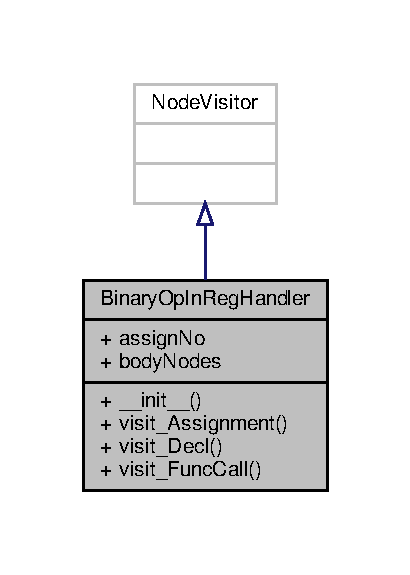
\includegraphics[width=197pt]{classPostProcessor_1_1Visitor_1_1BinaryOpInRegHandler__inherit__graph}
\end{center}
\end{figure}


Collaboration diagram for Binary\+Op\+In\+Reg\+Handler\+:\nopagebreak
\begin{figure}[H]
\begin{center}
\leavevmode
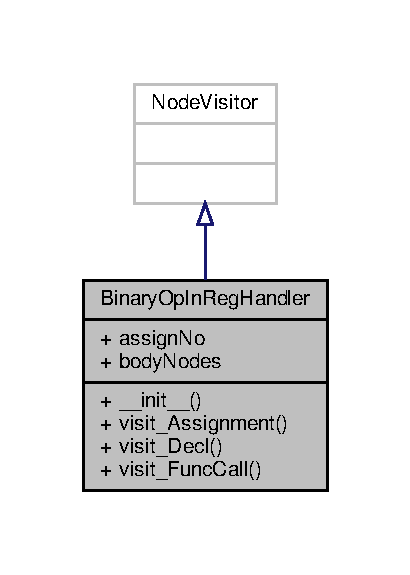
\includegraphics[width=197pt]{classPostProcessor_1_1Visitor_1_1BinaryOpInRegHandler__coll__graph}
\end{center}
\end{figure}
\subsection*{Public Member Functions}
\begin{DoxyCompactItemize}
\item 
def \hyperlink{classPostProcessor_1_1Visitor_1_1BinaryOpInRegHandler_a3328eb3718a1907a8a24087b075a2062}{\+\_\+\+\_\+init\+\_\+\+\_\+} (self, \hyperlink{classPostProcessor_1_1Visitor_1_1BinaryOpInRegHandler_afde190707204b09a99ff642a6afa5695}{body\+Nodes}, \hyperlink{classPostProcessor_1_1Visitor_1_1BinaryOpInRegHandler_a58eaabd0374c4bb1e31a844d27cc020e}{assign\+No})
\item 
def \hyperlink{classPostProcessor_1_1Visitor_1_1BinaryOpInRegHandler_adae6ad6f5b94c4acd95924bb3df9ebc8}{visit\+\_\+\+Assignment} (self, node)
\item 
def \hyperlink{classPostProcessor_1_1Visitor_1_1BinaryOpInRegHandler_a6568bead87923bbcaa593e5f226920f0}{visit\+\_\+\+Decl} (self, node)
\item 
def \hyperlink{classPostProcessor_1_1Visitor_1_1BinaryOpInRegHandler_a48e7baeee3968db14598ff72b6be63bd}{visit\+\_\+\+Func\+Call} (self, node)
\end{DoxyCompactItemize}
\subsection*{Public Attributes}
\begin{DoxyCompactItemize}
\item 
\hyperlink{classPostProcessor_1_1Visitor_1_1BinaryOpInRegHandler_a58eaabd0374c4bb1e31a844d27cc020e}{assign\+No}
\item 
\hyperlink{classPostProcessor_1_1Visitor_1_1BinaryOpInRegHandler_afde190707204b09a99ff642a6afa5695}{body\+Nodes}
\end{DoxyCompactItemize}


\subsection{Detailed Description}
\begin{DoxyVerb}Visitor for handling binary operations inside register function calls.

@param bodyNodes: A list to store transformed nodes.
@param assignNo: The current assignment number used for generating new variable names.
\end{DoxyVerb}
 

Definition at line 125 of file Visitor.\+py.



\subsection{Constructor \& Destructor Documentation}
\mbox{\Hypertarget{classPostProcessor_1_1Visitor_1_1BinaryOpInRegHandler_a3328eb3718a1907a8a24087b075a2062}\label{classPostProcessor_1_1Visitor_1_1BinaryOpInRegHandler_a3328eb3718a1907a8a24087b075a2062}} 
\index{Post\+Processor\+::\+Visitor\+::\+Binary\+Op\+In\+Reg\+Handler@{Post\+Processor\+::\+Visitor\+::\+Binary\+Op\+In\+Reg\+Handler}!\+\_\+\+\_\+init\+\_\+\+\_\+@{\+\_\+\+\_\+init\+\_\+\+\_\+}}
\index{\+\_\+\+\_\+init\+\_\+\+\_\+@{\+\_\+\+\_\+init\+\_\+\+\_\+}!Post\+Processor\+::\+Visitor\+::\+Binary\+Op\+In\+Reg\+Handler@{Post\+Processor\+::\+Visitor\+::\+Binary\+Op\+In\+Reg\+Handler}}
\subsubsection{\texorpdfstring{\+\_\+\+\_\+init\+\_\+\+\_\+()}{\_\_init\_\_()}}
{\footnotesize\ttfamily def \+\_\+\+\_\+init\+\_\+\+\_\+ (\begin{DoxyParamCaption}\item[{}]{self,  }\item[{}]{body\+Nodes,  }\item[{}]{assign\+No }\end{DoxyParamCaption})}

\begin{DoxyVerb}Initializes the BinaryOpInRegHandler.

@param bodyNodes: A list to store transformed nodes.
@param assignNo: The current assignment number used for generating new variable names.
\end{DoxyVerb}
 

Definition at line 132 of file Visitor.\+py.


\begin{DoxyCode}
132     \textcolor{keyword}{def }\_\_init\_\_(self,bodyNodes,assignNo):
133         \textcolor{stringliteral}{"""
}
134 \textcolor{stringliteral}{        Initializes the BinaryOpInRegHandler.
}
135 \textcolor{stringliteral}{
}
136 \textcolor{stringliteral}{        @param bodyNodes: A list to store transformed nodes.
}
137 \textcolor{stringliteral}{        @param assignNo: The current assignment number used for generating new variable names.
}
138 \textcolor{stringliteral}{        """}
139         self.bodyNodes = bodyNodes
140         self.assignNo = assignNo
141 
\end{DoxyCode}


\subsection{Member Function Documentation}
\mbox{\Hypertarget{classPostProcessor_1_1Visitor_1_1BinaryOpInRegHandler_adae6ad6f5b94c4acd95924bb3df9ebc8}\label{classPostProcessor_1_1Visitor_1_1BinaryOpInRegHandler_adae6ad6f5b94c4acd95924bb3df9ebc8}} 
\index{Post\+Processor\+::\+Visitor\+::\+Binary\+Op\+In\+Reg\+Handler@{Post\+Processor\+::\+Visitor\+::\+Binary\+Op\+In\+Reg\+Handler}!visit\+\_\+\+Assignment@{visit\+\_\+\+Assignment}}
\index{visit\+\_\+\+Assignment@{visit\+\_\+\+Assignment}!Post\+Processor\+::\+Visitor\+::\+Binary\+Op\+In\+Reg\+Handler@{Post\+Processor\+::\+Visitor\+::\+Binary\+Op\+In\+Reg\+Handler}}
\subsubsection{\texorpdfstring{visit\+\_\+\+Assignment()}{visit\_Assignment()}}
{\footnotesize\ttfamily def visit\+\_\+\+Assignment (\begin{DoxyParamCaption}\item[{}]{self,  }\item[{}]{node }\end{DoxyParamCaption})}

\begin{DoxyVerb}Visits assignment nodes and processes them based on their right-hand side type.

@param node: The assignment node to visit.
\end{DoxyVerb}
 

Definition at line 152 of file Visitor.\+py.


\begin{DoxyCode}
152     \textcolor{keyword}{def }visit\_Assignment(self,node):
153         \textcolor{stringliteral}{"""
}
154 \textcolor{stringliteral}{        Visits assignment nodes and processes them based on their right-hand side type.
}
155 \textcolor{stringliteral}{
}
156 \textcolor{stringliteral}{        @param node: The assignment node to visit.
}
157 \textcolor{stringliteral}{        """}
158         \textcolor{keywordflow}{if} \textcolor{keywordflow}{not} isinstance(node.rvalue,c\_ast.FuncCall):
159             self.bodyNodes.append(node)
160             \textcolor{keywordflow}{return}
161         self.generic\_visit(node)
162         self.bodyNodes.append(node)
163     
\end{DoxyCode}
\mbox{\Hypertarget{classPostProcessor_1_1Visitor_1_1BinaryOpInRegHandler_a6568bead87923bbcaa593e5f226920f0}\label{classPostProcessor_1_1Visitor_1_1BinaryOpInRegHandler_a6568bead87923bbcaa593e5f226920f0}} 
\index{Post\+Processor\+::\+Visitor\+::\+Binary\+Op\+In\+Reg\+Handler@{Post\+Processor\+::\+Visitor\+::\+Binary\+Op\+In\+Reg\+Handler}!visit\+\_\+\+Decl@{visit\+\_\+\+Decl}}
\index{visit\+\_\+\+Decl@{visit\+\_\+\+Decl}!Post\+Processor\+::\+Visitor\+::\+Binary\+Op\+In\+Reg\+Handler@{Post\+Processor\+::\+Visitor\+::\+Binary\+Op\+In\+Reg\+Handler}}
\subsubsection{\texorpdfstring{visit\+\_\+\+Decl()}{visit\_Decl()}}
{\footnotesize\ttfamily def visit\+\_\+\+Decl (\begin{DoxyParamCaption}\item[{}]{self,  }\item[{}]{node }\end{DoxyParamCaption})}

\begin{DoxyVerb}Visits declaration nodes and appends them to the body nodes list.

@param node: The declaration node to visit.
\end{DoxyVerb}
 

Definition at line 142 of file Visitor.\+py.


\begin{DoxyCode}
142     \textcolor{keyword}{def }visit\_Decl(self,node):
143         \textcolor{stringliteral}{"""
}
144 \textcolor{stringliteral}{        Visits declaration nodes and appends them to the body nodes list.
}
145 \textcolor{stringliteral}{
}
146 \textcolor{stringliteral}{        @param node: The declaration node to visit.
}
147 \textcolor{stringliteral}{        """}
148         \textcolor{keywordflow}{if} isinstance(node.type,c\_ast.TypeDecl):
149             self.bodyNodes.append(node)
150         \textcolor{keywordflow}{return}
151 
\end{DoxyCode}
\mbox{\Hypertarget{classPostProcessor_1_1Visitor_1_1BinaryOpInRegHandler_a48e7baeee3968db14598ff72b6be63bd}\label{classPostProcessor_1_1Visitor_1_1BinaryOpInRegHandler_a48e7baeee3968db14598ff72b6be63bd}} 
\index{Post\+Processor\+::\+Visitor\+::\+Binary\+Op\+In\+Reg\+Handler@{Post\+Processor\+::\+Visitor\+::\+Binary\+Op\+In\+Reg\+Handler}!visit\+\_\+\+Func\+Call@{visit\+\_\+\+Func\+Call}}
\index{visit\+\_\+\+Func\+Call@{visit\+\_\+\+Func\+Call}!Post\+Processor\+::\+Visitor\+::\+Binary\+Op\+In\+Reg\+Handler@{Post\+Processor\+::\+Visitor\+::\+Binary\+Op\+In\+Reg\+Handler}}
\subsubsection{\texorpdfstring{visit\+\_\+\+Func\+Call()}{visit\_FuncCall()}}
{\footnotesize\ttfamily def visit\+\_\+\+Func\+Call (\begin{DoxyParamCaption}\item[{}]{self,  }\item[{}]{node }\end{DoxyParamCaption})}

\begin{DoxyVerb}Visits function call nodes and processes binary operations within register function calls.

@param node: The function call node to visit.
\end{DoxyVerb}
 

Definition at line 164 of file Visitor.\+py.


\begin{DoxyCode}
164     \textcolor{keyword}{def }visit\_FuncCall(self,node):
165         \textcolor{stringliteral}{"""
}
166 \textcolor{stringliteral}{        Visits function call nodes and processes binary operations within register function calls.
}
167 \textcolor{stringliteral}{
}
168 \textcolor{stringliteral}{        @param node: The function call node to visit.
}
169 \textcolor{stringliteral}{        """}
170         currNode = node
171         \textcolor{keywordflow}{while} \hyperlink{namespacePostProcessor_1_1utils_a89d6f2461251261de6b862c69fe3c44a}{isRegCall}(currNode.args.exprs[0]):
172             currNode = currNode.args.exprs[0]
173         insideNode = currNode.args.exprs[0]
174         \textcolor{keywordflow}{if} isinstance(insideNode,c\_ast.BinaryOp):
175             \textcolor{keywordflow}{if} \hyperlink{namespacePostProcessor_1_1utils_a89d6f2461251261de6b862c69fe3c44a}{isRegCall}(insideNode.right) \textcolor{keywordflow}{or} \hyperlink{namespacePostProcessor_1_1utils_a89d6f2461251261de6b862c69fe3c44a}{isRegCall}(insideNode.left):
176                 varName = \hyperlink{namespacePostProcessor_1_1utils_a69c4094b747eccefbd43b8011b1c3626}{getNewVarName}(self.assignNo)
177                 self.assignNo += 2
178                 currNode.args.exprs[0] = c\_ast.ID(name=varName)
179                 self.bodyNodes.append(\hyperlink{namespaceastNodes_ae5e5c7f09a1586002b20db6d72f6d30b}{getDeclarationNode}(varName))
180                 self.bodyNodes.append(\hyperlink{namespaceastNodes_a2403f5d006e54f20e614226280cb6cbc}{getSimpleAssignmentNode}(lvalue=varName,rvalue=
      insideNode))
181 
\end{DoxyCode}
Here is the call graph for this function\+:\nopagebreak
\begin{figure}[H]
\begin{center}
\leavevmode
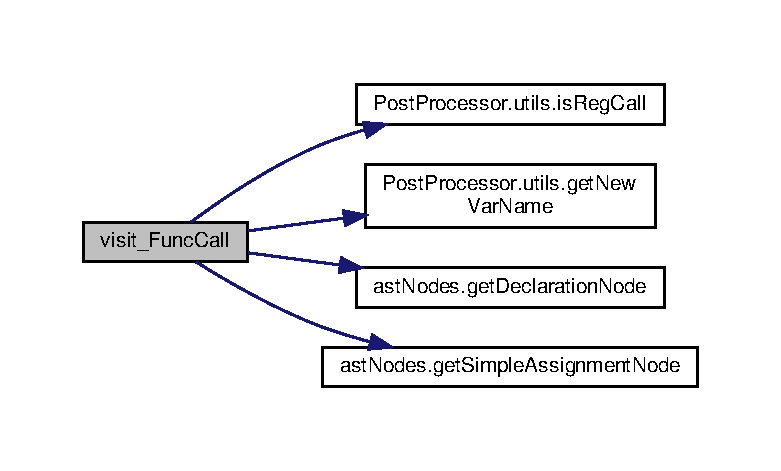
\includegraphics[width=350pt]{classPostProcessor_1_1Visitor_1_1BinaryOpInRegHandler_a48e7baeee3968db14598ff72b6be63bd_cgraph}
\end{center}
\end{figure}


\subsection{Member Data Documentation}
\mbox{\Hypertarget{classPostProcessor_1_1Visitor_1_1BinaryOpInRegHandler_a58eaabd0374c4bb1e31a844d27cc020e}\label{classPostProcessor_1_1Visitor_1_1BinaryOpInRegHandler_a58eaabd0374c4bb1e31a844d27cc020e}} 
\index{Post\+Processor\+::\+Visitor\+::\+Binary\+Op\+In\+Reg\+Handler@{Post\+Processor\+::\+Visitor\+::\+Binary\+Op\+In\+Reg\+Handler}!assign\+No@{assign\+No}}
\index{assign\+No@{assign\+No}!Post\+Processor\+::\+Visitor\+::\+Binary\+Op\+In\+Reg\+Handler@{Post\+Processor\+::\+Visitor\+::\+Binary\+Op\+In\+Reg\+Handler}}
\subsubsection{\texorpdfstring{assign\+No}{assignNo}}
{\footnotesize\ttfamily assign\+No}



Definition at line 140 of file Visitor.\+py.

\mbox{\Hypertarget{classPostProcessor_1_1Visitor_1_1BinaryOpInRegHandler_afde190707204b09a99ff642a6afa5695}\label{classPostProcessor_1_1Visitor_1_1BinaryOpInRegHandler_afde190707204b09a99ff642a6afa5695}} 
\index{Post\+Processor\+::\+Visitor\+::\+Binary\+Op\+In\+Reg\+Handler@{Post\+Processor\+::\+Visitor\+::\+Binary\+Op\+In\+Reg\+Handler}!body\+Nodes@{body\+Nodes}}
\index{body\+Nodes@{body\+Nodes}!Post\+Processor\+::\+Visitor\+::\+Binary\+Op\+In\+Reg\+Handler@{Post\+Processor\+::\+Visitor\+::\+Binary\+Op\+In\+Reg\+Handler}}
\subsubsection{\texorpdfstring{body\+Nodes}{bodyNodes}}
{\footnotesize\ttfamily body\+Nodes}



Definition at line 139 of file Visitor.\+py.



The documentation for this class was generated from the following file\+:\begin{DoxyCompactItemize}
\item 
Post\+Processor/\hyperlink{Visitor_8py}{Visitor.\+py}\end{DoxyCompactItemize}

\hypertarget{classVisitors_1_1ConstantMerger}{}\section{Constant\+Merger Class Reference}
\label{classVisitors_1_1ConstantMerger}\index{Constant\+Merger@{Constant\+Merger}}


Inheritance diagram for Constant\+Merger\+:\nopagebreak
\begin{figure}[H]
\begin{center}
\leavevmode
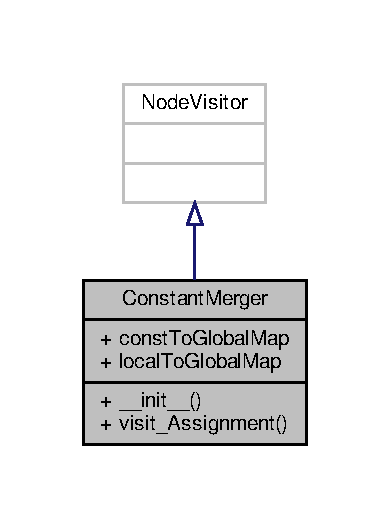
\includegraphics[width=187pt]{classVisitors_1_1ConstantMerger__inherit__graph}
\end{center}
\end{figure}


Collaboration diagram for Constant\+Merger\+:\nopagebreak
\begin{figure}[H]
\begin{center}
\leavevmode
\includegraphics[width=187pt]{classVisitors_1_1ConstantMerger__coll__graph}
\end{center}
\end{figure}
\subsection*{Public Member Functions}
\begin{DoxyCompactItemize}
\item 
def \hyperlink{classVisitors_1_1ConstantMerger_af7415dba49be733196acc4fe0274fb1f}{\+\_\+\+\_\+init\+\_\+\+\_\+} (self, \hyperlink{classVisitors_1_1ConstantMerger_a09a8838a26160063ff7f70a6d8ca53f8}{const\+To\+Global\+Map}, \hyperlink{classVisitors_1_1ConstantMerger_a6aa7ad73b0ac6388e786fd93172a1421}{local\+To\+Global\+Map})
\item 
def \hyperlink{classVisitors_1_1ConstantMerger_adae6ad6f5b94c4acd95924bb3df9ebc8}{visit\+\_\+\+Assignment} (self, node)
\end{DoxyCompactItemize}
\subsection*{Public Attributes}
\begin{DoxyCompactItemize}
\item 
\hyperlink{classVisitors_1_1ConstantMerger_a09a8838a26160063ff7f70a6d8ca53f8}{const\+To\+Global\+Map}
\item 
\hyperlink{classVisitors_1_1ConstantMerger_a6aa7ad73b0ac6388e786fd93172a1421}{local\+To\+Global\+Map}
\end{DoxyCompactItemize}


\subsection{Detailed Description}
\begin{DoxyVerb}@brief Merges constants into global variables and updates local variable mappings.

This visitor consolidates constant values into global variables and updates local variable mappings accordingly.

@param constToGlobalMap: Mapping of constant values to global variable names.
@type constToGlobalMap: dict
@param localToGlobalMap: Mapping of local variable names to global variable names.
@type localToGlobalMap: dict
\end{DoxyVerb}
 

Definition at line 232 of file Visitors.\+py.



\subsection{Constructor \& Destructor Documentation}
\mbox{\Hypertarget{classVisitors_1_1ConstantMerger_af7415dba49be733196acc4fe0274fb1f}\label{classVisitors_1_1ConstantMerger_af7415dba49be733196acc4fe0274fb1f}} 
\index{Visitors\+::\+Constant\+Merger@{Visitors\+::\+Constant\+Merger}!\+\_\+\+\_\+init\+\_\+\+\_\+@{\+\_\+\+\_\+init\+\_\+\+\_\+}}
\index{\+\_\+\+\_\+init\+\_\+\+\_\+@{\+\_\+\+\_\+init\+\_\+\+\_\+}!Visitors\+::\+Constant\+Merger@{Visitors\+::\+Constant\+Merger}}
\subsubsection{\texorpdfstring{\+\_\+\+\_\+init\+\_\+\+\_\+()}{\_\_init\_\_()}}
{\footnotesize\ttfamily def \+\_\+\+\_\+init\+\_\+\+\_\+ (\begin{DoxyParamCaption}\item[{}]{self,  }\item[{}]{const\+To\+Global\+Map,  }\item[{}]{local\+To\+Global\+Map }\end{DoxyParamCaption})}



Definition at line 243 of file Visitors.\+py.


\begin{DoxyCode}
243     \textcolor{keyword}{def }\_\_init\_\_(self,constToGlobalMap,localToGlobalMap):
244         self.constToGlobalMap = constToGlobalMap
245         self.localToGlobalMap = localToGlobalMap
246 
\end{DoxyCode}


\subsection{Member Function Documentation}
\mbox{\Hypertarget{classVisitors_1_1ConstantMerger_adae6ad6f5b94c4acd95924bb3df9ebc8}\label{classVisitors_1_1ConstantMerger_adae6ad6f5b94c4acd95924bb3df9ebc8}} 
\index{Visitors\+::\+Constant\+Merger@{Visitors\+::\+Constant\+Merger}!visit\+\_\+\+Assignment@{visit\+\_\+\+Assignment}}
\index{visit\+\_\+\+Assignment@{visit\+\_\+\+Assignment}!Visitors\+::\+Constant\+Merger@{Visitors\+::\+Constant\+Merger}}
\subsubsection{\texorpdfstring{visit\+\_\+\+Assignment()}{visit\_Assignment()}}
{\footnotesize\ttfamily def visit\+\_\+\+Assignment (\begin{DoxyParamCaption}\item[{}]{self,  }\item[{}]{node }\end{DoxyParamCaption})}

\begin{DoxyVerb}@brief Converts constant values in assignments to global variable names.

@param node: The assignment node being processed.
@type node: pycparser.c_ast.Assignment
\end{DoxyVerb}
 

Definition at line 261 of file Visitors.\+py.


\begin{DoxyCode}
261     \textcolor{keyword}{def }visit\_Assignment(self,node):
262         \textcolor{stringliteral}{"""
}
263 \textcolor{stringliteral}{        @brief Converts constant values in assignments to global variable names.
}
264 \textcolor{stringliteral}{
}
265 \textcolor{stringliteral}{        @param node: The assignment node being processed.
}
266 \textcolor{stringliteral}{        @type node: pycparser.c\_ast.Assignment
}
267 \textcolor{stringliteral}{        """}
268         \textcolor{keywordflow}{if} isinstance(node.rvalue,c\_ast.Constant):
269             constValue = node.rvalue.value
270             idConstValue = self.\_\_getNameForConstants(constValue)
271             \textcolor{keywordflow}{if} constValue \textcolor{keywordflow}{not} \textcolor{keywordflow}{in} self.constToGlobalMap:
272                 self.constToGlobalMap[constValue] = idConstValue
273             self.localToGlobalMap[node.lvalue.name] = idConstValue
274         \textcolor{keywordflow}{if} isinstance(node.rvalue,c\_ast.BinaryOp):
275             constName = node.rvalue.right.name
276             node.rvalue.right.name = self.localToGlobalMap[constName]
277 
\end{DoxyCode}
Here is the call graph for this function\+:\nopagebreak
\begin{figure}[H]
\begin{center}
\leavevmode
\includegraphics[width=334pt]{classVisitors_1_1ConstantMerger_adae6ad6f5b94c4acd95924bb3df9ebc8_cgraph}
\end{center}
\end{figure}


\subsection{Member Data Documentation}
\mbox{\Hypertarget{classVisitors_1_1ConstantMerger_a09a8838a26160063ff7f70a6d8ca53f8}\label{classVisitors_1_1ConstantMerger_a09a8838a26160063ff7f70a6d8ca53f8}} 
\index{Visitors\+::\+Constant\+Merger@{Visitors\+::\+Constant\+Merger}!const\+To\+Global\+Map@{const\+To\+Global\+Map}}
\index{const\+To\+Global\+Map@{const\+To\+Global\+Map}!Visitors\+::\+Constant\+Merger@{Visitors\+::\+Constant\+Merger}}
\subsubsection{\texorpdfstring{const\+To\+Global\+Map}{constToGlobalMap}}
{\footnotesize\ttfamily const\+To\+Global\+Map}



Definition at line 244 of file Visitors.\+py.

\mbox{\Hypertarget{classVisitors_1_1ConstantMerger_a6aa7ad73b0ac6388e786fd93172a1421}\label{classVisitors_1_1ConstantMerger_a6aa7ad73b0ac6388e786fd93172a1421}} 
\index{Visitors\+::\+Constant\+Merger@{Visitors\+::\+Constant\+Merger}!local\+To\+Global\+Map@{local\+To\+Global\+Map}}
\index{local\+To\+Global\+Map@{local\+To\+Global\+Map}!Visitors\+::\+Constant\+Merger@{Visitors\+::\+Constant\+Merger}}
\subsubsection{\texorpdfstring{local\+To\+Global\+Map}{localToGlobalMap}}
{\footnotesize\ttfamily local\+To\+Global\+Map}



Definition at line 245 of file Visitors.\+py.



The documentation for this class was generated from the following file\+:\begin{DoxyCompactItemize}
\item 
Inliner/\hyperlink{Visitors_8py}{Visitors.\+py}\end{DoxyCompactItemize}

\hypertarget{classVisitors_1_1ConstToVar}{}\section{Const\+To\+Var Class Reference}
\label{classVisitors_1_1ConstToVar}\index{Const\+To\+Var@{Const\+To\+Var}}


Inheritance diagram for Const\+To\+Var\+:\nopagebreak
\begin{figure}[H]
\begin{center}
\leavevmode
\includegraphics[width=187pt]{classVisitors_1_1ConstToVar__inherit__graph}
\end{center}
\end{figure}


Collaboration diagram for Const\+To\+Var\+:\nopagebreak
\begin{figure}[H]
\begin{center}
\leavevmode
\includegraphics[width=187pt]{classVisitors_1_1ConstToVar__coll__graph}
\end{center}
\end{figure}
\subsection*{Public Member Functions}
\begin{DoxyCompactItemize}
\item 
def \hyperlink{classVisitors_1_1ConstToVar_adae6ad6f5b94c4acd95924bb3df9ebc8}{visit\+\_\+\+Assignment} (self, node)
\item 
def \hyperlink{classVisitors_1_1ConstToVar_a6329fbf13e2d22de5384fbca843113b8}{visit\+\_\+\+Binary\+Op} (self, node)
\end{DoxyCompactItemize}


\subsection{Detailed Description}
\begin{DoxyVerb}@brief Converts constant values in the AST to variable names.

This visitor replaces constant values in assignments and binary operations with corresponding variable names.\end{DoxyVerb}
 

Definition at line 198 of file Visitors.\+py.



\subsection{Member Function Documentation}
\mbox{\Hypertarget{classVisitors_1_1ConstToVar_adae6ad6f5b94c4acd95924bb3df9ebc8}\label{classVisitors_1_1ConstToVar_adae6ad6f5b94c4acd95924bb3df9ebc8}} 
\index{Visitors\+::\+Const\+To\+Var@{Visitors\+::\+Const\+To\+Var}!visit\+\_\+\+Assignment@{visit\+\_\+\+Assignment}}
\index{visit\+\_\+\+Assignment@{visit\+\_\+\+Assignment}!Visitors\+::\+Const\+To\+Var@{Visitors\+::\+Const\+To\+Var}}
\subsubsection{\texorpdfstring{visit\+\_\+\+Assignment()}{visit\_Assignment()}}
{\footnotesize\ttfamily def visit\+\_\+\+Assignment (\begin{DoxyParamCaption}\item[{}]{self,  }\item[{}]{node }\end{DoxyParamCaption})}

\begin{DoxyVerb}@brief Replaces constant values in assignment operations with variable names.

@param node: The assignment node being processed.
@type node: pycparser.c_ast.Assignment
\end{DoxyVerb}
 

Definition at line 205 of file Visitors.\+py.


\begin{DoxyCode}
205     \textcolor{keyword}{def }visit\_Assignment(self,node):
206         \textcolor{stringliteral}{"""
}
207 \textcolor{stringliteral}{        @brief Replaces constant values in assignment operations with variable names.
}
208 \textcolor{stringliteral}{
}
209 \textcolor{stringliteral}{        @param node: The assignment node being processed.
}
210 \textcolor{stringliteral}{        @type node: pycparser.c\_ast.Assignment
}
211 \textcolor{stringliteral}{        """}
212         \textcolor{keywordflow}{if} isinstance(node.rvalue,c\_ast.Constant):
213             constName = node.rvalue.value
214             node.rvalue = c\_ast.ID(name=\textcolor{stringliteral}{"dec\_"} + constName + \textcolor{stringliteral}{"\_inp"})
215             \textcolor{keywordflow}{return}
216         \textcolor{keywordflow}{else}:
217             self.generic\_visit(node)
\end{DoxyCode}
\mbox{\Hypertarget{classVisitors_1_1ConstToVar_a6329fbf13e2d22de5384fbca843113b8}\label{classVisitors_1_1ConstToVar_a6329fbf13e2d22de5384fbca843113b8}} 
\index{Visitors\+::\+Const\+To\+Var@{Visitors\+::\+Const\+To\+Var}!visit\+\_\+\+Binary\+Op@{visit\+\_\+\+Binary\+Op}}
\index{visit\+\_\+\+Binary\+Op@{visit\+\_\+\+Binary\+Op}!Visitors\+::\+Const\+To\+Var@{Visitors\+::\+Const\+To\+Var}}
\subsubsection{\texorpdfstring{visit\+\_\+\+Binary\+Op()}{visit\_BinaryOp()}}
{\footnotesize\ttfamily def visit\+\_\+\+Binary\+Op (\begin{DoxyParamCaption}\item[{}]{self,  }\item[{}]{node }\end{DoxyParamCaption})}

\begin{DoxyVerb}@brief Replaces constant values in binary operations with variable names.

@param node: The binary operation node being processed.
@type node: pycparser.c_ast.BinaryOp
\end{DoxyVerb}
 

Definition at line 218 of file Visitors.\+py.


\begin{DoxyCode}
218     \textcolor{keyword}{def }visit\_BinaryOp(self,node):
219         \textcolor{stringliteral}{"""
}
220 \textcolor{stringliteral}{        @brief Replaces constant values in binary operations with variable names.
}
221 \textcolor{stringliteral}{
}
222 \textcolor{stringliteral}{        @param node: The binary operation node being processed.
}
223 \textcolor{stringliteral}{        @type node: pycparser.c\_ast.BinaryOp
}
224 \textcolor{stringliteral}{        """}
225         \textcolor{keywordflow}{if} isinstance(node.right,c\_ast.Constant):
226             constName = node.right.value
227             node.right = c\_ast.ID(name=\textcolor{stringliteral}{"dec\_"} + constName + \textcolor{stringliteral}{"\_inp"})
228         \textcolor{keywordflow}{if} isinstance(node.left,c\_ast.Constant):
229             constName = node.left.value
230             node.left = c\_ast.ID(name=\textcolor{stringliteral}{"dec\_"} + constName + \textcolor{stringliteral}{"\_inp"})
231 
\end{DoxyCode}


The documentation for this class was generated from the following file\+:\begin{DoxyCompactItemize}
\item 
Inliner/\hyperlink{Visitors_8py}{Visitors.\+py}\end{DoxyCompactItemize}

\hypertarget{classVisitors_1_1DeclVisitor}{}\section{Decl\+Visitor Class Reference}
\label{classVisitors_1_1DeclVisitor}\index{Decl\+Visitor@{Decl\+Visitor}}


Inheritance diagram for Decl\+Visitor\+:\nopagebreak
\begin{figure}[H]
\begin{center}
\leavevmode
\includegraphics[width=157pt]{classVisitors_1_1DeclVisitor__inherit__graph}
\end{center}
\end{figure}


Collaboration diagram for Decl\+Visitor\+:\nopagebreak
\begin{figure}[H]
\begin{center}
\leavevmode
\includegraphics[width=157pt]{classVisitors_1_1DeclVisitor__coll__graph}
\end{center}
\end{figure}
\subsection*{Public Member Functions}
\begin{DoxyCompactItemize}
\item 
def \hyperlink{classVisitors_1_1DeclVisitor_a0997355e72bfeeb0091a98ad9b380dd6}{\+\_\+\+\_\+init\+\_\+\+\_\+} (self, \hyperlink{classVisitors_1_1DeclVisitor_a3c14dac355802b0266a75f0ee417c14b}{array\+Map}=None, \hyperlink{classVisitors_1_1DeclVisitor_a83d838e3813fb5999c0492e0d9474bd9}{ast}=None)
\item 
def \hyperlink{classVisitors_1_1DeclVisitor_a9e0516fab7677e7c20e7761b239d5a88}{store\+Array} (self, node)
\item 
def \hyperlink{classVisitors_1_1DeclVisitor_a6568bead87923bbcaa593e5f226920f0}{visit\+\_\+\+Decl} (self, node)
\end{DoxyCompactItemize}
\subsection*{Public Attributes}
\begin{DoxyCompactItemize}
\item 
\hyperlink{classVisitors_1_1DeclVisitor_a3c14dac355802b0266a75f0ee417c14b}{array\+Map}
\item 
\hyperlink{classVisitors_1_1DeclVisitor_a83d838e3813fb5999c0492e0d9474bd9}{ast}
\end{DoxyCompactItemize}


\subsection{Detailed Description}
\begin{DoxyVerb}@brief Visits declaration nodes to store array initialization values.

This visitor collects initialization values for array declarations and stores them in a map.

@param arrayMap: Dictionary to store array names and their corresponding values.
@type arrayMap: dict
@param ast: The Abstract Syntax Tree being processed.
@type ast: pycparser.c_ast.FileAST
\end{DoxyVerb}
 

Definition at line 57 of file Visitors.\+py.



\subsection{Constructor \& Destructor Documentation}
\mbox{\Hypertarget{classVisitors_1_1DeclVisitor_a0997355e72bfeeb0091a98ad9b380dd6}\label{classVisitors_1_1DeclVisitor_a0997355e72bfeeb0091a98ad9b380dd6}} 
\index{Visitors\+::\+Decl\+Visitor@{Visitors\+::\+Decl\+Visitor}!\+\_\+\+\_\+init\+\_\+\+\_\+@{\+\_\+\+\_\+init\+\_\+\+\_\+}}
\index{\+\_\+\+\_\+init\+\_\+\+\_\+@{\+\_\+\+\_\+init\+\_\+\+\_\+}!Visitors\+::\+Decl\+Visitor@{Visitors\+::\+Decl\+Visitor}}
\subsubsection{\texorpdfstring{\+\_\+\+\_\+init\+\_\+\+\_\+()}{\_\_init\_\_()}}
{\footnotesize\ttfamily def \+\_\+\+\_\+init\+\_\+\+\_\+ (\begin{DoxyParamCaption}\item[{}]{self,  }\item[{}]{array\+Map = {\ttfamily None},  }\item[{}]{ast = {\ttfamily None} }\end{DoxyParamCaption})}



Definition at line 68 of file Visitors.\+py.


\begin{DoxyCode}
68     \textcolor{keyword}{def }\_\_init\_\_(self,arrayMap = None,ast = None):
69         self.arrayMap = arrayMap
70         self.ast = ast
71 
\end{DoxyCode}


\subsection{Member Function Documentation}
\mbox{\Hypertarget{classVisitors_1_1DeclVisitor_a9e0516fab7677e7c20e7761b239d5a88}\label{classVisitors_1_1DeclVisitor_a9e0516fab7677e7c20e7761b239d5a88}} 
\index{Visitors\+::\+Decl\+Visitor@{Visitors\+::\+Decl\+Visitor}!store\+Array@{store\+Array}}
\index{store\+Array@{store\+Array}!Visitors\+::\+Decl\+Visitor@{Visitors\+::\+Decl\+Visitor}}
\subsubsection{\texorpdfstring{store\+Array()}{storeArray()}}
{\footnotesize\ttfamily def store\+Array (\begin{DoxyParamCaption}\item[{}]{self,  }\item[{}]{node }\end{DoxyParamCaption})}

\begin{DoxyVerb}@brief Stores the values of an array declaration in the array map.

@param node: The array declaration node to process.
@type node: pycparser.c_ast.Decl
\end{DoxyVerb}
 

Definition at line 72 of file Visitors.\+py.


\begin{DoxyCode}
72     \textcolor{keyword}{def }storeArray(self,node):
73         \textcolor{stringliteral}{"""
}
74 \textcolor{stringliteral}{        @brief Stores the values of an array declaration in the array map.
}
75 \textcolor{stringliteral}{
}
76 \textcolor{stringliteral}{        @param node: The array declaration node to process.
}
77 \textcolor{stringliteral}{        @type node: pycparser.c\_ast.Decl
}
78 \textcolor{stringliteral}{        """}
79         arrName = node.name
80         contents = []
81         \textcolor{keywordflow}{for} item \textcolor{keywordflow}{in} node.init.exprs:
82             \textcolor{keywordflow}{if} item.value.startswith(\textcolor{stringliteral}{"0x"}):
83                 decVal = int(item.value[2:],16)
84             \textcolor{keywordflow}{else}:
85                 decVal = int(item.value)
86             contents.append(decVal)
87         self.arrayMap[arrName] = contents
88 
\end{DoxyCode}
Here is the caller graph for this function\+:\nopagebreak
\begin{figure}[H]
\begin{center}
\leavevmode
\includegraphics[width=238pt]{classVisitors_1_1DeclVisitor_a9e0516fab7677e7c20e7761b239d5a88_icgraph}
\end{center}
\end{figure}
\mbox{\Hypertarget{classVisitors_1_1DeclVisitor_a6568bead87923bbcaa593e5f226920f0}\label{classVisitors_1_1DeclVisitor_a6568bead87923bbcaa593e5f226920f0}} 
\index{Visitors\+::\+Decl\+Visitor@{Visitors\+::\+Decl\+Visitor}!visit\+\_\+\+Decl@{visit\+\_\+\+Decl}}
\index{visit\+\_\+\+Decl@{visit\+\_\+\+Decl}!Visitors\+::\+Decl\+Visitor@{Visitors\+::\+Decl\+Visitor}}
\subsubsection{\texorpdfstring{visit\+\_\+\+Decl()}{visit\_Decl()}}
{\footnotesize\ttfamily def visit\+\_\+\+Decl (\begin{DoxyParamCaption}\item[{}]{self,  }\item[{}]{node }\end{DoxyParamCaption})}

\begin{DoxyVerb}@brief Processes declaration nodes to handle array declarations.

Calls the storeArray method if the declaration is an array.

@param node: The declaration node being visited.
@type node: pycparser.c_ast.Decl
\end{DoxyVerb}
 

Definition at line 89 of file Visitors.\+py.


\begin{DoxyCode}
89     \textcolor{keyword}{def }visit\_Decl(self,node):
90         \textcolor{stringliteral}{"""
}
91 \textcolor{stringliteral}{        @brief Processes declaration nodes to handle array declarations.
}
92 \textcolor{stringliteral}{
}
93 \textcolor{stringliteral}{        Calls the storeArray method if the declaration is an array.
}
94 \textcolor{stringliteral}{
}
95 \textcolor{stringliteral}{        @param node: The declaration node being visited.
}
96 \textcolor{stringliteral}{        @type node: pycparser.c\_ast.Decl
}
97 \textcolor{stringliteral}{        """}
98         declType = node.type.type
99 
100         \textcolor{keywordflow}{if} isinstance(node.type,c\_ast.ArrayDecl):
101             self.storeArray(node)
102 
\end{DoxyCode}
Here is the call graph for this function\+:\nopagebreak
\begin{figure}[H]
\begin{center}
\leavevmode
\includegraphics[width=238pt]{classVisitors_1_1DeclVisitor_a6568bead87923bbcaa593e5f226920f0_cgraph}
\end{center}
\end{figure}


\subsection{Member Data Documentation}
\mbox{\Hypertarget{classVisitors_1_1DeclVisitor_a3c14dac355802b0266a75f0ee417c14b}\label{classVisitors_1_1DeclVisitor_a3c14dac355802b0266a75f0ee417c14b}} 
\index{Visitors\+::\+Decl\+Visitor@{Visitors\+::\+Decl\+Visitor}!array\+Map@{array\+Map}}
\index{array\+Map@{array\+Map}!Visitors\+::\+Decl\+Visitor@{Visitors\+::\+Decl\+Visitor}}
\subsubsection{\texorpdfstring{array\+Map}{arrayMap}}
{\footnotesize\ttfamily array\+Map}



Definition at line 69 of file Visitors.\+py.

\mbox{\Hypertarget{classVisitors_1_1DeclVisitor_a83d838e3813fb5999c0492e0d9474bd9}\label{classVisitors_1_1DeclVisitor_a83d838e3813fb5999c0492e0d9474bd9}} 
\index{Visitors\+::\+Decl\+Visitor@{Visitors\+::\+Decl\+Visitor}!ast@{ast}}
\index{ast@{ast}!Visitors\+::\+Decl\+Visitor@{Visitors\+::\+Decl\+Visitor}}
\subsubsection{\texorpdfstring{ast}{ast}}
{\footnotesize\ttfamily ast}



Definition at line 70 of file Visitors.\+py.



The documentation for this class was generated from the following file\+:\begin{DoxyCompactItemize}
\item 
Inliner/\hyperlink{Visitors_8py}{Visitors.\+py}\end{DoxyCompactItemize}

\hypertarget{classDiGraph_1_1DiGraph}{}\section{Di\+Graph Class Reference}
\label{classDiGraph_1_1DiGraph}\index{Di\+Graph@{Di\+Graph}}


Collaboration diagram for Di\+Graph\+:\nopagebreak
\begin{figure}[H]
\begin{center}
\leavevmode
\includegraphics[width=188pt]{classDiGraph_1_1DiGraph__coll__graph}
\end{center}
\end{figure}
\subsection*{Public Member Functions}
\begin{DoxyCompactItemize}
\item 
def \hyperlink{classDiGraph_1_1DiGraph_ae64f0875afe3067b97ba370b354b9213}{\+\_\+\+\_\+init\+\_\+\+\_\+} (self)
\item 
def \hyperlink{classDiGraph_1_1DiGraph_ab064bb6af6f4d1916413e2ab9ef9cdb4}{add\+Edge\+Between} (self, f1, f2)
\item 
def \hyperlink{classDiGraph_1_1DiGraph_a9e00e5549f827c5cbba05adaa49d7e57}{add\+Function} (self, f\+Name)
\item 
def \hyperlink{classDiGraph_1_1DiGraph_a02f36c0ebca9e0e4fab9591c7d43130b}{get\+Indegree\+Of} (self, f\+Name)
\item 
def \hyperlink{classDiGraph_1_1DiGraph_ab37be01195a3d4a4cb7c992114e93219}{topo\+Sort} (self)
\end{DoxyCompactItemize}
\subsection*{Public Attributes}
\begin{DoxyCompactItemize}
\item 
\hyperlink{classDiGraph_1_1DiGraph_af9bd6d4d8ecd1b0563241fd648435e14}{num\+Nodes}
\end{DoxyCompactItemize}


\subsection{Detailed Description}
\begin{DoxyVerb}@brief A class representing a directed graph with nodes and edges.

This class provides methods for adding nodes and edges, retrieving in-degrees, and performing topological sorting.
\end{DoxyVerb}
 

Definition at line 5 of file Di\+Graph.\+py.



\subsection{Constructor \& Destructor Documentation}
\mbox{\Hypertarget{classDiGraph_1_1DiGraph_ae64f0875afe3067b97ba370b354b9213}\label{classDiGraph_1_1DiGraph_ae64f0875afe3067b97ba370b354b9213}} 
\index{Di\+Graph\+::\+Di\+Graph@{Di\+Graph\+::\+Di\+Graph}!\+\_\+\+\_\+init\+\_\+\+\_\+@{\+\_\+\+\_\+init\+\_\+\+\_\+}}
\index{\+\_\+\+\_\+init\+\_\+\+\_\+@{\+\_\+\+\_\+init\+\_\+\+\_\+}!Di\+Graph\+::\+Di\+Graph@{Di\+Graph\+::\+Di\+Graph}}
\subsubsection{\texorpdfstring{\+\_\+\+\_\+init\+\_\+\+\_\+()}{\_\_init\_\_()}}
{\footnotesize\ttfamily def \+\_\+\+\_\+init\+\_\+\+\_\+ (\begin{DoxyParamCaption}\item[{}]{self }\end{DoxyParamCaption})}

\begin{DoxyVerb}@brief Initializes an empty directed graph.

Sets up internal data structures to keep track of nodes, adjacency lists, and in-degrees.
\end{DoxyVerb}
 

Definition at line 11 of file Di\+Graph.\+py.


\begin{DoxyCode}
11     \textcolor{keyword}{def }\_\_init\_\_(self):
12         \textcolor{stringliteral}{"""
}
13 \textcolor{stringliteral}{        @brief Initializes an empty directed graph.
}
14 \textcolor{stringliteral}{
}
15 \textcolor{stringliteral}{        Sets up internal data structures to keep track of nodes, adjacency lists, and in-degrees.
}
16 \textcolor{stringliteral}{        """}
17         self.\_\_inEdges = []
18         self.\_\_functionIndexMap = \{\}
19         self.\_\_indexFunctionMap = \{\}
20         self.\_\_adjacencyList = []
21         self.numNodes = 0
22     
\end{DoxyCode}


\subsection{Member Function Documentation}
\mbox{\Hypertarget{classDiGraph_1_1DiGraph_ab064bb6af6f4d1916413e2ab9ef9cdb4}\label{classDiGraph_1_1DiGraph_ab064bb6af6f4d1916413e2ab9ef9cdb4}} 
\index{Di\+Graph\+::\+Di\+Graph@{Di\+Graph\+::\+Di\+Graph}!add\+Edge\+Between@{add\+Edge\+Between}}
\index{add\+Edge\+Between@{add\+Edge\+Between}!Di\+Graph\+::\+Di\+Graph@{Di\+Graph\+::\+Di\+Graph}}
\subsubsection{\texorpdfstring{add\+Edge\+Between()}{addEdgeBetween()}}
{\footnotesize\ttfamily def add\+Edge\+Between (\begin{DoxyParamCaption}\item[{}]{self,  }\item[{}]{f1,  }\item[{}]{f2 }\end{DoxyParamCaption})}

\begin{DoxyVerb}@brief Adds a directed edge from function f1 to function f2.

Updates the adjacency list and the in-degree of function f2.

@param f1: The name of the source function.
@type f1: str
@param f2: The name of the target function.
@type f2: str

@raises KeyError: If either function name is not present in the graph.
\end{DoxyVerb}
 

Definition at line 41 of file Di\+Graph.\+py.


\begin{DoxyCode}
41     \textcolor{keyword}{def }addEdgeBetween(self,f1,f2):
42         \textcolor{stringliteral}{"""
}
43 \textcolor{stringliteral}{        @brief Adds a directed edge from function f1 to function f2.
}
44 \textcolor{stringliteral}{
}
45 \textcolor{stringliteral}{        Updates the adjacency list and the in-degree of function f2.
}
46 \textcolor{stringliteral}{
}
47 \textcolor{stringliteral}{        @param f1: The name of the source function.
}
48 \textcolor{stringliteral}{        @type f1: str
}
49 \textcolor{stringliteral}{        @param f2: The name of the target function.
}
50 \textcolor{stringliteral}{        @type f2: str
}
51 \textcolor{stringliteral}{
}
52 \textcolor{stringliteral}{        @raises KeyError: If either function name is not present in the graph.
}
53 \textcolor{stringliteral}{        """}
54         f1Index = self.\_\_functionIndexMap[f1]
55         f2Index = self.\_\_functionIndexMap[f2]
56         \textcolor{keywordflow}{if} f2Index \textcolor{keywordflow}{not} \textcolor{keywordflow}{in} self.\_\_adjacencyList[f1Index]:
57             self.\_\_adjacencyList[f1Index].append(f2Index)
58             self.\_\_inEdges[f2Index] += 1
59     
\end{DoxyCode}
\mbox{\Hypertarget{classDiGraph_1_1DiGraph_a9e00e5549f827c5cbba05adaa49d7e57}\label{classDiGraph_1_1DiGraph_a9e00e5549f827c5cbba05adaa49d7e57}} 
\index{Di\+Graph\+::\+Di\+Graph@{Di\+Graph\+::\+Di\+Graph}!add\+Function@{add\+Function}}
\index{add\+Function@{add\+Function}!Di\+Graph\+::\+Di\+Graph@{Di\+Graph\+::\+Di\+Graph}}
\subsubsection{\texorpdfstring{add\+Function()}{addFunction()}}
{\footnotesize\ttfamily def add\+Function (\begin{DoxyParamCaption}\item[{}]{self,  }\item[{}]{f\+Name }\end{DoxyParamCaption})}

\begin{DoxyVerb}@brief Adds a function as a node to the graph.

If the function is not already present, it adds it and initializes its adjacency list and in-degree.

@param fName: The name of the function to be added as a node.
@type fName: str

@raises KeyError: If the function name is already in the graph.
\end{DoxyVerb}
 

Definition at line 23 of file Di\+Graph.\+py.


\begin{DoxyCode}
23     \textcolor{keyword}{def }addFunction(self,fName):
24         \textcolor{stringliteral}{"""
}
25 \textcolor{stringliteral}{        @brief Adds a function as a node to the graph.
}
26 \textcolor{stringliteral}{
}
27 \textcolor{stringliteral}{        If the function is not already present, it adds it and initializes its adjacency list and
       in-degree.
}
28 \textcolor{stringliteral}{
}
29 \textcolor{stringliteral}{        @param fName: The name of the function to be added as a node.
}
30 \textcolor{stringliteral}{        @type fName: str
}
31 \textcolor{stringliteral}{
}
32 \textcolor{stringliteral}{        @raises KeyError: If the function name is already in the graph.
}
33 \textcolor{stringliteral}{        """}
34         \textcolor{keywordflow}{if} fName \textcolor{keywordflow}{not} \textcolor{keywordflow}{in} self.\_\_functionIndexMap:
35             self.\_\_functionIndexMap[fName] = self.numNodes
36             self.\_\_indexFunctionMap[self.numNodes] = fName
37             self.numNodes += 1
38             self.\_\_adjacencyList.append([])
39             self.\_\_inEdges.append(0)
40     
\end{DoxyCode}
\mbox{\Hypertarget{classDiGraph_1_1DiGraph_a02f36c0ebca9e0e4fab9591c7d43130b}\label{classDiGraph_1_1DiGraph_a02f36c0ebca9e0e4fab9591c7d43130b}} 
\index{Di\+Graph\+::\+Di\+Graph@{Di\+Graph\+::\+Di\+Graph}!get\+Indegree\+Of@{get\+Indegree\+Of}}
\index{get\+Indegree\+Of@{get\+Indegree\+Of}!Di\+Graph\+::\+Di\+Graph@{Di\+Graph\+::\+Di\+Graph}}
\subsubsection{\texorpdfstring{get\+Indegree\+Of()}{getIndegreeOf()}}
{\footnotesize\ttfamily def get\+Indegree\+Of (\begin{DoxyParamCaption}\item[{}]{self,  }\item[{}]{f\+Name }\end{DoxyParamCaption})}

\begin{DoxyVerb}@brief Retrieves the in-degree of the specified function.

@param fName: The name of the function whose in-degree is to be retrieved.
@type fName: str

@return: The in-degree of the specified function.
@rtype: int

@raises KeyError: If the function name is not present in the graph.
\end{DoxyVerb}
 

Definition at line 60 of file Di\+Graph.\+py.


\begin{DoxyCode}
60     \textcolor{keyword}{def }getIndegreeOf(self,fName):
61         \textcolor{stringliteral}{"""
}
62 \textcolor{stringliteral}{        @brief Retrieves the in-degree of the specified function.
}
63 \textcolor{stringliteral}{
}
64 \textcolor{stringliteral}{        @param fName: The name of the function whose in-degree is to be retrieved.
}
65 \textcolor{stringliteral}{        @type fName: str
}
66 \textcolor{stringliteral}{
}
67 \textcolor{stringliteral}{        @return: The in-degree of the specified function.
}
68 \textcolor{stringliteral}{        @rtype: int
}
69 \textcolor{stringliteral}{
}
70 \textcolor{stringliteral}{        @raises KeyError: If the function name is not present in the graph.
}
71 \textcolor{stringliteral}{        """}
72         \textcolor{keywordflow}{return} self.\_\_inEdges[self.\_\_functionIndexMap[fName]]
73     
\end{DoxyCode}
\mbox{\Hypertarget{classDiGraph_1_1DiGraph_ab37be01195a3d4a4cb7c992114e93219}\label{classDiGraph_1_1DiGraph_ab37be01195a3d4a4cb7c992114e93219}} 
\index{Di\+Graph\+::\+Di\+Graph@{Di\+Graph\+::\+Di\+Graph}!topo\+Sort@{topo\+Sort}}
\index{topo\+Sort@{topo\+Sort}!Di\+Graph\+::\+Di\+Graph@{Di\+Graph\+::\+Di\+Graph}}
\subsubsection{\texorpdfstring{topo\+Sort()}{topoSort()}}
{\footnotesize\ttfamily def topo\+Sort (\begin{DoxyParamCaption}\item[{}]{self }\end{DoxyParamCaption})}

\begin{DoxyVerb}@brief Performs a topological sort on the graph.

Uses Kahn's algorithm to return a list of nodes in topologically sorted order.

@return: A list of function names in topologically sorted order.
@rtype: list of str
\end{DoxyVerb}
 

Definition at line 74 of file Di\+Graph.\+py.


\begin{DoxyCode}
74     \textcolor{keyword}{def }topoSort(self):
75         \textcolor{stringliteral}{"""
}
76 \textcolor{stringliteral}{        @brief Performs a topological sort on the graph.
}
77 \textcolor{stringliteral}{
}
78 \textcolor{stringliteral}{        Uses Kahn's algorithm to return a list of nodes in topologically sorted order.
}
79 \textcolor{stringliteral}{
}
80 \textcolor{stringliteral}{        @return: A list of function names in topologically sorted order.
}
81 \textcolor{stringliteral}{        @rtype: list of str
}
82 \textcolor{stringliteral}{        """}
83         q = deque()
84         inEdges = copy.deepcopy(self.\_\_inEdges)
85         \textcolor{keywordflow}{for} index \textcolor{keywordflow}{in} range(self.numNodes):
86             if(inEdges[index] == 0):
87                 q.append(index)
88         sortedList = []
89         \textcolor{keywordflow}{while} q:
90             node = q.popleft()
91             sortedList.append(self.\_\_indexFunctionMap[node])
92             \textcolor{keywordflow}{for} adj \textcolor{keywordflow}{in} self.\_\_adjacencyList[node]:
93                 inEdges[adj] -= 1
94                 if(inEdges[adj] == 0):
95                     q.append(adj)
96         \textcolor{keywordflow}{return} sortedList
97 
98 \end{DoxyCode}


\subsection{Member Data Documentation}
\mbox{\Hypertarget{classDiGraph_1_1DiGraph_af9bd6d4d8ecd1b0563241fd648435e14}\label{classDiGraph_1_1DiGraph_af9bd6d4d8ecd1b0563241fd648435e14}} 
\index{Di\+Graph\+::\+Di\+Graph@{Di\+Graph\+::\+Di\+Graph}!num\+Nodes@{num\+Nodes}}
\index{num\+Nodes@{num\+Nodes}!Di\+Graph\+::\+Di\+Graph@{Di\+Graph\+::\+Di\+Graph}}
\subsubsection{\texorpdfstring{num\+Nodes}{numNodes}}
{\footnotesize\ttfamily num\+Nodes}



Definition at line 21 of file Di\+Graph.\+py.



The documentation for this class was generated from the following file\+:\begin{DoxyCompactItemize}
\item 
Inliner/\hyperlink{DiGraph_8py}{Di\+Graph.\+py}\end{DoxyCompactItemize}

\hypertarget{classVisitors_1_1FunctionVisitor}{}\section{Function\+Visitor Class Reference}
\label{classVisitors_1_1FunctionVisitor}\index{Function\+Visitor@{Function\+Visitor}}


Inheritance diagram for Function\+Visitor\+:\nopagebreak
\begin{figure}[H]
\begin{center}
\leavevmode
\includegraphics[width=174pt]{classVisitors_1_1FunctionVisitor__inherit__graph}
\end{center}
\end{figure}


Collaboration diagram for Function\+Visitor\+:\nopagebreak
\begin{figure}[H]
\begin{center}
\leavevmode
\includegraphics[width=174pt]{classVisitors_1_1FunctionVisitor__coll__graph}
\end{center}
\end{figure}
\subsection*{Public Member Functions}
\begin{DoxyCompactItemize}
\item 
def \hyperlink{classVisitors_1_1FunctionVisitor_ac775ee34451fdfa742b318538164070e}{\+\_\+\+\_\+init\+\_\+\+\_\+}
\item 
def \hyperlink{classVisitors_1_1FunctionVisitor_a48e7baeee3968db14598ff72b6be63bd}{visit\+\_\+\+Func\+Call} (self, node)
\end{DoxyCompactItemize}
\subsection*{Public Attributes}
\begin{DoxyCompactItemize}
\item 
\hyperlink{classVisitors_1_1FunctionVisitor_a773d3c032f7708247230d5a2e169fe4d}{di\+Graph}
\item 
\hyperlink{classVisitors_1_1FunctionVisitor_ab781b0aec3a9de0632eb6afda1e10288}{function\+Name}
\end{DoxyCompactItemize}


\subsection{Detailed Description}
\begin{DoxyVerb}@brief Visits function call nodes in the AST and updates the dependency graph.

This visitor traverses the function call nodes in the AST to build a dependency graph of functions.

@param diGraph: The directed graph that tracks function dependencies.
@type diGraph: DiGraph
@param functionName: The name of the current function being processed.
@type functionName: str
\end{DoxyVerb}
 

Definition at line 4 of file Visitors.\+py.



\subsection{Constructor \& Destructor Documentation}
\mbox{\Hypertarget{classVisitors_1_1FunctionVisitor_ac775ee34451fdfa742b318538164070e}\label{classVisitors_1_1FunctionVisitor_ac775ee34451fdfa742b318538164070e}} 
\index{Visitors\+::\+Function\+Visitor@{Visitors\+::\+Function\+Visitor}!\+\_\+\+\_\+init\+\_\+\+\_\+@{\+\_\+\+\_\+init\+\_\+\+\_\+}}
\index{\+\_\+\+\_\+init\+\_\+\+\_\+@{\+\_\+\+\_\+init\+\_\+\+\_\+}!Visitors\+::\+Function\+Visitor@{Visitors\+::\+Function\+Visitor}}
\subsubsection{\texorpdfstring{\+\_\+\+\_\+init\+\_\+\+\_\+()}{\_\_init\_\_()}}
{\footnotesize\ttfamily def \+\_\+\+\_\+init\+\_\+\+\_\+ (\begin{DoxyParamCaption}\item[{}]{self,  }\item[{}]{di\+Graph }\end{DoxyParamCaption})}



Definition at line 15 of file Visitors.\+py.


\begin{DoxyCode}
15     \textcolor{keyword}{def }\_\_init\_\_(self,diGraph : DiGraph,functionName):
16         self.diGraph = diGraph
17         self.functionName = functionName
\end{DoxyCode}


\subsection{Member Function Documentation}
\mbox{\Hypertarget{classVisitors_1_1FunctionVisitor_a48e7baeee3968db14598ff72b6be63bd}\label{classVisitors_1_1FunctionVisitor_a48e7baeee3968db14598ff72b6be63bd}} 
\index{Visitors\+::\+Function\+Visitor@{Visitors\+::\+Function\+Visitor}!visit\+\_\+\+Func\+Call@{visit\+\_\+\+Func\+Call}}
\index{visit\+\_\+\+Func\+Call@{visit\+\_\+\+Func\+Call}!Visitors\+::\+Function\+Visitor@{Visitors\+::\+Function\+Visitor}}
\subsubsection{\texorpdfstring{visit\+\_\+\+Func\+Call()}{visit\_FuncCall()}}
{\footnotesize\ttfamily def visit\+\_\+\+Func\+Call (\begin{DoxyParamCaption}\item[{}]{self,  }\item[{}]{node }\end{DoxyParamCaption})}

\begin{DoxyVerb}@brief Processes function call nodes and updates the function dependency graph.

Adds the function called to the graph and creates an edge from the called function to the current function.

@param node: The function call node being visited.
@type node: pycparser.c_ast.FuncCall
\end{DoxyVerb}
 

Definition at line 18 of file Visitors.\+py.


\begin{DoxyCode}
18     \textcolor{keyword}{def }visit\_FuncCall(self,node):
19         \textcolor{stringliteral}{"""
}
20 \textcolor{stringliteral}{        @brief Processes function call nodes and updates the function dependency graph.
}
21 \textcolor{stringliteral}{
}
22 \textcolor{stringliteral}{        Adds the function called to the graph and creates an edge from the called function to the current
       function.
}
23 \textcolor{stringliteral}{
}
24 \textcolor{stringliteral}{        @param node: The function call node being visited.
}
25 \textcolor{stringliteral}{        @type node: pycparser.c\_ast.FuncCall
}
26 \textcolor{stringliteral}{        """}
27         \textcolor{keywordflow}{if} node.name.name != \textcolor{stringliteral}{'reg'}:
28             self.diGraph.addFunction(node.name.name)
29             self.diGraph.addEdgeBetween(node.name.name,self.functionName)
30 
\end{DoxyCode}


\subsection{Member Data Documentation}
\mbox{\Hypertarget{classVisitors_1_1FunctionVisitor_a773d3c032f7708247230d5a2e169fe4d}\label{classVisitors_1_1FunctionVisitor_a773d3c032f7708247230d5a2e169fe4d}} 
\index{Visitors\+::\+Function\+Visitor@{Visitors\+::\+Function\+Visitor}!di\+Graph@{di\+Graph}}
\index{di\+Graph@{di\+Graph}!Visitors\+::\+Function\+Visitor@{Visitors\+::\+Function\+Visitor}}
\subsubsection{\texorpdfstring{di\+Graph}{diGraph}}
{\footnotesize\ttfamily di\+Graph}



Definition at line 16 of file Visitors.\+py.

\mbox{\Hypertarget{classVisitors_1_1FunctionVisitor_ab781b0aec3a9de0632eb6afda1e10288}\label{classVisitors_1_1FunctionVisitor_ab781b0aec3a9de0632eb6afda1e10288}} 
\index{Visitors\+::\+Function\+Visitor@{Visitors\+::\+Function\+Visitor}!function\+Name@{function\+Name}}
\index{function\+Name@{function\+Name}!Visitors\+::\+Function\+Visitor@{Visitors\+::\+Function\+Visitor}}
\subsubsection{\texorpdfstring{function\+Name}{functionName}}
{\footnotesize\ttfamily function\+Name}



Definition at line 17 of file Visitors.\+py.



The documentation for this class was generated from the following file\+:\begin{DoxyCompactItemize}
\item 
Inliner/\hyperlink{Visitors_8py}{Visitors.\+py}\end{DoxyCompactItemize}

\hypertarget{classVisitors_1_1IdVisitor}{}\section{Id\+Visitor Class Reference}
\label{classVisitors_1_1IdVisitor}\index{Id\+Visitor@{Id\+Visitor}}


Inheritance diagram for Id\+Visitor\+:\nopagebreak
\begin{figure}[H]
\begin{center}
\leavevmode
\includegraphics[width=185pt]{classVisitors_1_1IdVisitor__inherit__graph}
\end{center}
\end{figure}


Collaboration diagram for Id\+Visitor\+:\nopagebreak
\begin{figure}[H]
\begin{center}
\leavevmode
\includegraphics[width=185pt]{classVisitors_1_1IdVisitor__coll__graph}
\end{center}
\end{figure}
\subsection*{Public Member Functions}
\begin{DoxyCompactItemize}
\item 
def \hyperlink{classVisitors_1_1IdVisitor_a649fc0ef07aae1d9fc3a510d3fe85c7f}{\+\_\+\+\_\+init\+\_\+\+\_\+} (self, \hyperlink{classVisitors_1_1IdVisitor_a976941a4c7ae422cebf58ddfd2e8b479}{argument\+Map}, \hyperlink{classVisitors_1_1IdVisitor_ad7cca8103c884420bac50cbb68183848}{local\+Variables\+Map})
\item 
def \hyperlink{classVisitors_1_1IdVisitor_a876b22ca4502c2197e9881ebf8fb6288}{visit\+\_\+\+ID} (self, node)
\end{DoxyCompactItemize}
\subsection*{Public Attributes}
\begin{DoxyCompactItemize}
\item 
\hyperlink{classVisitors_1_1IdVisitor_a976941a4c7ae422cebf58ddfd2e8b479}{argument\+Map}
\item 
\hyperlink{classVisitors_1_1IdVisitor_ad7cca8103c884420bac50cbb68183848}{local\+Variables\+Map}
\end{DoxyCompactItemize}


\subsection{Detailed Description}
\begin{DoxyVerb}@brief Visits identifier nodes and updates their names based on provided mappings.

This visitor changes the names of identifiers according to the argument and local variable mappings.

@param argumentMap: Mapping of argument names to new names.
@type argumentMap: dict
@param localVariablesMap: Mapping of local variable names to new names.
@type localVariablesMap: dict
\end{DoxyVerb}
 

Definition at line 126 of file Visitors.\+py.



\subsection{Constructor \& Destructor Documentation}
\mbox{\Hypertarget{classVisitors_1_1IdVisitor_a649fc0ef07aae1d9fc3a510d3fe85c7f}\label{classVisitors_1_1IdVisitor_a649fc0ef07aae1d9fc3a510d3fe85c7f}} 
\index{Visitors\+::\+Id\+Visitor@{Visitors\+::\+Id\+Visitor}!\+\_\+\+\_\+init\+\_\+\+\_\+@{\+\_\+\+\_\+init\+\_\+\+\_\+}}
\index{\+\_\+\+\_\+init\+\_\+\+\_\+@{\+\_\+\+\_\+init\+\_\+\+\_\+}!Visitors\+::\+Id\+Visitor@{Visitors\+::\+Id\+Visitor}}
\subsubsection{\texorpdfstring{\+\_\+\+\_\+init\+\_\+\+\_\+()}{\_\_init\_\_()}}
{\footnotesize\ttfamily def \+\_\+\+\_\+init\+\_\+\+\_\+ (\begin{DoxyParamCaption}\item[{}]{self,  }\item[{}]{argument\+Map,  }\item[{}]{local\+Variables\+Map }\end{DoxyParamCaption})}



Definition at line 137 of file Visitors.\+py.


\begin{DoxyCode}
137     \textcolor{keyword}{def }\_\_init\_\_(self,argumentMap,localVariablesMap):
138         self.localVariablesMap = localVariablesMap
139         self.argumentMap = argumentMap
\end{DoxyCode}


\subsection{Member Function Documentation}
\mbox{\Hypertarget{classVisitors_1_1IdVisitor_a876b22ca4502c2197e9881ebf8fb6288}\label{classVisitors_1_1IdVisitor_a876b22ca4502c2197e9881ebf8fb6288}} 
\index{Visitors\+::\+Id\+Visitor@{Visitors\+::\+Id\+Visitor}!visit\+\_\+\+ID@{visit\+\_\+\+ID}}
\index{visit\+\_\+\+ID@{visit\+\_\+\+ID}!Visitors\+::\+Id\+Visitor@{Visitors\+::\+Id\+Visitor}}
\subsubsection{\texorpdfstring{visit\+\_\+\+I\+D()}{visit\_ID()}}
{\footnotesize\ttfamily def visit\+\_\+\+ID (\begin{DoxyParamCaption}\item[{}]{self,  }\item[{}]{node }\end{DoxyParamCaption})}

\begin{DoxyVerb}@brief Updates identifier names based on argument and local variable mappings.

@param node: The identifier node to be updated.
@type node: pycparser.c_ast.ID
\end{DoxyVerb}
 

Definition at line 140 of file Visitors.\+py.


\begin{DoxyCode}
140     \textcolor{keyword}{def }visit\_ID(self, node):
141         \textcolor{stringliteral}{"""
}
142 \textcolor{stringliteral}{        @brief Updates identifier names based on argument and local variable mappings.
}
143 \textcolor{stringliteral}{
}
144 \textcolor{stringliteral}{        @param node: The identifier node to be updated.
}
145 \textcolor{stringliteral}{        @type node: pycparser.c\_ast.ID
}
146 \textcolor{stringliteral}{        """}
147         \textcolor{keywordflow}{if} node.name \textcolor{keywordflow}{in} self.argumentMap:
148             node.name = self.argumentMap[node.name]
149         \textcolor{keywordflow}{if} node.name \textcolor{keywordflow}{in} self.localVariablesMap:
150             node.name = self.localVariablesMap[node.name]
151 
\end{DoxyCode}


\subsection{Member Data Documentation}
\mbox{\Hypertarget{classVisitors_1_1IdVisitor_a976941a4c7ae422cebf58ddfd2e8b479}\label{classVisitors_1_1IdVisitor_a976941a4c7ae422cebf58ddfd2e8b479}} 
\index{Visitors\+::\+Id\+Visitor@{Visitors\+::\+Id\+Visitor}!argument\+Map@{argument\+Map}}
\index{argument\+Map@{argument\+Map}!Visitors\+::\+Id\+Visitor@{Visitors\+::\+Id\+Visitor}}
\subsubsection{\texorpdfstring{argument\+Map}{argumentMap}}
{\footnotesize\ttfamily argument\+Map}



Definition at line 139 of file Visitors.\+py.

\mbox{\Hypertarget{classVisitors_1_1IdVisitor_ad7cca8103c884420bac50cbb68183848}\label{classVisitors_1_1IdVisitor_ad7cca8103c884420bac50cbb68183848}} 
\index{Visitors\+::\+Id\+Visitor@{Visitors\+::\+Id\+Visitor}!local\+Variables\+Map@{local\+Variables\+Map}}
\index{local\+Variables\+Map@{local\+Variables\+Map}!Visitors\+::\+Id\+Visitor@{Visitors\+::\+Id\+Visitor}}
\subsubsection{\texorpdfstring{local\+Variables\+Map}{localVariablesMap}}
{\footnotesize\ttfamily local\+Variables\+Map}



Definition at line 138 of file Visitors.\+py.



The documentation for this class was generated from the following file\+:\begin{DoxyCompactItemize}
\item 
Inliner/\hyperlink{Visitors_8py}{Visitors.\+py}\end{DoxyCompactItemize}

\hypertarget{classVisitors_1_1InputParamModifier}{}\section{Input\+Param\+Modifier Class Reference}
\label{classVisitors_1_1InputParamModifier}\index{Input\+Param\+Modifier@{Input\+Param\+Modifier}}


Inheritance diagram for Input\+Param\+Modifier\+:\nopagebreak
\begin{figure}[H]
\begin{center}
\leavevmode
\includegraphics[width=183pt]{classVisitors_1_1InputParamModifier__inherit__graph}
\end{center}
\end{figure}


Collaboration diagram for Input\+Param\+Modifier\+:\nopagebreak
\begin{figure}[H]
\begin{center}
\leavevmode
\includegraphics[width=183pt]{classVisitors_1_1InputParamModifier__coll__graph}
\end{center}
\end{figure}
\subsection*{Public Member Functions}
\begin{DoxyCompactItemize}
\item 
def \hyperlink{classVisitors_1_1InputParamModifier_a1e3784a2a4444d63be94163c3a8508d5}{\+\_\+\+\_\+init\+\_\+\+\_\+} (self, \hyperlink{classVisitors_1_1InputParamModifier_a4ca1ea41a954d2675cd3c1915c9568e9}{changed\+Input\+Map})
\item 
def \hyperlink{classVisitors_1_1InputParamModifier_a876b22ca4502c2197e9881ebf8fb6288}{visit\+\_\+\+ID} (self, node)
\end{DoxyCompactItemize}
\subsection*{Public Attributes}
\begin{DoxyCompactItemize}
\item 
\hyperlink{classVisitors_1_1InputParamModifier_a4ca1ea41a954d2675cd3c1915c9568e9}{changed\+Input\+Map}
\end{DoxyCompactItemize}


\subsection{Detailed Description}
\begin{DoxyVerb}@brief Modifies input parameter names based on a mapping.

This visitor updates the names of input parameters according to a provided mapping.

@param changedInputMap: Mapping of original input parameter names to new names.
@type changedInputMap: dict
\end{DoxyVerb}
 

Definition at line 103 of file Visitors.\+py.



\subsection{Constructor \& Destructor Documentation}
\mbox{\Hypertarget{classVisitors_1_1InputParamModifier_a1e3784a2a4444d63be94163c3a8508d5}\label{classVisitors_1_1InputParamModifier_a1e3784a2a4444d63be94163c3a8508d5}} 
\index{Visitors\+::\+Input\+Param\+Modifier@{Visitors\+::\+Input\+Param\+Modifier}!\+\_\+\+\_\+init\+\_\+\+\_\+@{\+\_\+\+\_\+init\+\_\+\+\_\+}}
\index{\+\_\+\+\_\+init\+\_\+\+\_\+@{\+\_\+\+\_\+init\+\_\+\+\_\+}!Visitors\+::\+Input\+Param\+Modifier@{Visitors\+::\+Input\+Param\+Modifier}}
\subsubsection{\texorpdfstring{\+\_\+\+\_\+init\+\_\+\+\_\+()}{\_\_init\_\_()}}
{\footnotesize\ttfamily def \+\_\+\+\_\+init\+\_\+\+\_\+ (\begin{DoxyParamCaption}\item[{}]{self,  }\item[{}]{changed\+Input\+Map }\end{DoxyParamCaption})}



Definition at line 112 of file Visitors.\+py.


\begin{DoxyCode}
112     \textcolor{keyword}{def }\_\_init\_\_(self,changedInputMap):
113         self.changedInputMap = changedInputMap
\end{DoxyCode}


\subsection{Member Function Documentation}
\mbox{\Hypertarget{classVisitors_1_1InputParamModifier_a876b22ca4502c2197e9881ebf8fb6288}\label{classVisitors_1_1InputParamModifier_a876b22ca4502c2197e9881ebf8fb6288}} 
\index{Visitors\+::\+Input\+Param\+Modifier@{Visitors\+::\+Input\+Param\+Modifier}!visit\+\_\+\+ID@{visit\+\_\+\+ID}}
\index{visit\+\_\+\+ID@{visit\+\_\+\+ID}!Visitors\+::\+Input\+Param\+Modifier@{Visitors\+::\+Input\+Param\+Modifier}}
\subsubsection{\texorpdfstring{visit\+\_\+\+I\+D()}{visit\_ID()}}
{\footnotesize\ttfamily def visit\+\_\+\+ID (\begin{DoxyParamCaption}\item[{}]{self,  }\item[{}]{node }\end{DoxyParamCaption})}

\begin{DoxyVerb}@brief Updates input parameter names based on the mapping.

Replaces the parameter name with the new name from the mapping if it exists.

@param node: The identifier node representing an input parameter.
@type node: pycparser.c_ast.ID
\end{DoxyVerb}
 

Definition at line 114 of file Visitors.\+py.


\begin{DoxyCode}
114     \textcolor{keyword}{def }visit\_ID(self,node):
115         \textcolor{stringliteral}{"""
}
116 \textcolor{stringliteral}{        @brief Updates input parameter names based on the mapping.
}
117 \textcolor{stringliteral}{
}
118 \textcolor{stringliteral}{        Replaces the parameter name with the new name from the mapping if it exists.
}
119 \textcolor{stringliteral}{
}
120 \textcolor{stringliteral}{        @param node: The identifier node representing an input parameter.
}
121 \textcolor{stringliteral}{        @type node: pycparser.c\_ast.ID
}
122 \textcolor{stringliteral}{        """}
123         \textcolor{keywordflow}{if} node.name \textcolor{keywordflow}{in} self.changedInputMap:
124             node.name = self.changedInputMap[node.name]
125 
\end{DoxyCode}


\subsection{Member Data Documentation}
\mbox{\Hypertarget{classVisitors_1_1InputParamModifier_a4ca1ea41a954d2675cd3c1915c9568e9}\label{classVisitors_1_1InputParamModifier_a4ca1ea41a954d2675cd3c1915c9568e9}} 
\index{Visitors\+::\+Input\+Param\+Modifier@{Visitors\+::\+Input\+Param\+Modifier}!changed\+Input\+Map@{changed\+Input\+Map}}
\index{changed\+Input\+Map@{changed\+Input\+Map}!Visitors\+::\+Input\+Param\+Modifier@{Visitors\+::\+Input\+Param\+Modifier}}
\subsubsection{\texorpdfstring{changed\+Input\+Map}{changedInputMap}}
{\footnotesize\ttfamily changed\+Input\+Map}



Definition at line 113 of file Visitors.\+py.



The documentation for this class was generated from the following file\+:\begin{DoxyCompactItemize}
\item 
Inliner/\hyperlink{Visitors_8py}{Visitors.\+py}\end{DoxyCompactItemize}

\hypertarget{classVisitors_1_1LocalVariablesModifier}{}\section{Local\+Variables\+Modifier Class Reference}
\label{classVisitors_1_1LocalVariablesModifier}\index{Local\+Variables\+Modifier@{Local\+Variables\+Modifier}}


Inheritance diagram for Local\+Variables\+Modifier\+:\nopagebreak
\begin{figure}[H]
\begin{center}
\leavevmode
\includegraphics[width=195pt]{classVisitors_1_1LocalVariablesModifier__inherit__graph}
\end{center}
\end{figure}


Collaboration diagram for Local\+Variables\+Modifier\+:\nopagebreak
\begin{figure}[H]
\begin{center}
\leavevmode
\includegraphics[width=195pt]{classVisitors_1_1LocalVariablesModifier__coll__graph}
\end{center}
\end{figure}
\subsection*{Public Member Functions}
\begin{DoxyCompactItemize}
\item 
def \hyperlink{classVisitors_1_1LocalVariablesModifier_a914dde44586c626013d9734045573409}{\+\_\+\+\_\+init\+\_\+\+\_\+} (self, \hyperlink{classVisitors_1_1LocalVariablesModifier_af117185a96147e67251924514b93a25e}{local\+Variables}, \hyperlink{classVisitors_1_1LocalVariablesModifier_a5a5ccf2ed83be1d582eba6e7797690a5}{f\+Name})
\item 
def \hyperlink{classVisitors_1_1LocalVariablesModifier_a876b22ca4502c2197e9881ebf8fb6288}{visit\+\_\+\+ID} (self, node)
\end{DoxyCompactItemize}
\subsection*{Public Attributes}
\begin{DoxyCompactItemize}
\item 
\hyperlink{classVisitors_1_1LocalVariablesModifier_a5a5ccf2ed83be1d582eba6e7797690a5}{f\+Name}
\item 
\hyperlink{classVisitors_1_1LocalVariablesModifier_af117185a96147e67251924514b93a25e}{local\+Variables}
\end{DoxyCompactItemize}


\subsection{Detailed Description}
\begin{DoxyVerb}@brief Modifies local variable names by appending the function name.

This visitor updates the names of local variables by appending the function name to ensure uniqueness.

@param localVariables: List of local variable names to be modified.
@type localVariables: list of str
@param fName: The name of the function to append to local variable names.
@type fName: str
\end{DoxyVerb}
 

Definition at line 31 of file Visitors.\+py.



\subsection{Constructor \& Destructor Documentation}
\mbox{\Hypertarget{classVisitors_1_1LocalVariablesModifier_a914dde44586c626013d9734045573409}\label{classVisitors_1_1LocalVariablesModifier_a914dde44586c626013d9734045573409}} 
\index{Visitors\+::\+Local\+Variables\+Modifier@{Visitors\+::\+Local\+Variables\+Modifier}!\+\_\+\+\_\+init\+\_\+\+\_\+@{\+\_\+\+\_\+init\+\_\+\+\_\+}}
\index{\+\_\+\+\_\+init\+\_\+\+\_\+@{\+\_\+\+\_\+init\+\_\+\+\_\+}!Visitors\+::\+Local\+Variables\+Modifier@{Visitors\+::\+Local\+Variables\+Modifier}}
\subsubsection{\texorpdfstring{\+\_\+\+\_\+init\+\_\+\+\_\+()}{\_\_init\_\_()}}
{\footnotesize\ttfamily def \+\_\+\+\_\+init\+\_\+\+\_\+ (\begin{DoxyParamCaption}\item[{}]{self,  }\item[{}]{local\+Variables,  }\item[{}]{f\+Name }\end{DoxyParamCaption})}



Definition at line 42 of file Visitors.\+py.


\begin{DoxyCode}
42     \textcolor{keyword}{def }\_\_init\_\_(self,localVariables,fName):
43         self.localVariables = localVariables
44         self.fName = fName
\end{DoxyCode}


\subsection{Member Function Documentation}
\mbox{\Hypertarget{classVisitors_1_1LocalVariablesModifier_a876b22ca4502c2197e9881ebf8fb6288}\label{classVisitors_1_1LocalVariablesModifier_a876b22ca4502c2197e9881ebf8fb6288}} 
\index{Visitors\+::\+Local\+Variables\+Modifier@{Visitors\+::\+Local\+Variables\+Modifier}!visit\+\_\+\+ID@{visit\+\_\+\+ID}}
\index{visit\+\_\+\+ID@{visit\+\_\+\+ID}!Visitors\+::\+Local\+Variables\+Modifier@{Visitors\+::\+Local\+Variables\+Modifier}}
\subsubsection{\texorpdfstring{visit\+\_\+\+I\+D()}{visit\_ID()}}
{\footnotesize\ttfamily def visit\+\_\+\+ID (\begin{DoxyParamCaption}\item[{}]{self,  }\item[{}]{node }\end{DoxyParamCaption})}

\begin{DoxyVerb}@brief Updates local variable names with function name suffix.

Appends the function name to the local variable name if it is found in the list of local variables.

@param node: The identifier node representing a local variable.
@type node: pycparser.c_ast.ID
\end{DoxyVerb}
 

Definition at line 45 of file Visitors.\+py.


\begin{DoxyCode}
45     \textcolor{keyword}{def }visit\_ID(self,node):
46         \textcolor{stringliteral}{"""
}
47 \textcolor{stringliteral}{        @brief Updates local variable names with function name suffix.
}
48 \textcolor{stringliteral}{
}
49 \textcolor{stringliteral}{        Appends the function name to the local variable name if it is found in the list of local
       variables.
}
50 \textcolor{stringliteral}{
}
51 \textcolor{stringliteral}{        @param node: The identifier node representing a local variable.
}
52 \textcolor{stringliteral}{        @type node: pycparser.c\_ast.ID
}
53 \textcolor{stringliteral}{        """}
54         if(node.name \textcolor{keywordflow}{in} self.localVariables):
55             node.name = node.name + \textcolor{stringliteral}{'\_'} + self.fName
56 
\end{DoxyCode}


\subsection{Member Data Documentation}
\mbox{\Hypertarget{classVisitors_1_1LocalVariablesModifier_a5a5ccf2ed83be1d582eba6e7797690a5}\label{classVisitors_1_1LocalVariablesModifier_a5a5ccf2ed83be1d582eba6e7797690a5}} 
\index{Visitors\+::\+Local\+Variables\+Modifier@{Visitors\+::\+Local\+Variables\+Modifier}!f\+Name@{f\+Name}}
\index{f\+Name@{f\+Name}!Visitors\+::\+Local\+Variables\+Modifier@{Visitors\+::\+Local\+Variables\+Modifier}}
\subsubsection{\texorpdfstring{f\+Name}{fName}}
{\footnotesize\ttfamily f\+Name}



Definition at line 44 of file Visitors.\+py.

\mbox{\Hypertarget{classVisitors_1_1LocalVariablesModifier_af117185a96147e67251924514b93a25e}\label{classVisitors_1_1LocalVariablesModifier_af117185a96147e67251924514b93a25e}} 
\index{Visitors\+::\+Local\+Variables\+Modifier@{Visitors\+::\+Local\+Variables\+Modifier}!local\+Variables@{local\+Variables}}
\index{local\+Variables@{local\+Variables}!Visitors\+::\+Local\+Variables\+Modifier@{Visitors\+::\+Local\+Variables\+Modifier}}
\subsubsection{\texorpdfstring{local\+Variables}{localVariables}}
{\footnotesize\ttfamily local\+Variables}



Definition at line 43 of file Visitors.\+py.



The documentation for this class was generated from the following file\+:\begin{DoxyCompactItemize}
\item 
Inliner/\hyperlink{Visitors_8py}{Visitors.\+py}\end{DoxyCompactItemize}

\hypertarget{classPostProcessor_1_1Visitor_1_1NegationVisitor}{}\section{Negation\+Visitor Class Reference}
\label{classPostProcessor_1_1Visitor_1_1NegationVisitor}\index{Negation\+Visitor@{Negation\+Visitor}}


Inheritance diagram for Negation\+Visitor\+:\nopagebreak
\begin{figure}[H]
\begin{center}
\leavevmode
\includegraphics[width=201pt]{classPostProcessor_1_1Visitor_1_1NegationVisitor__inherit__graph}
\end{center}
\end{figure}


Collaboration diagram for Negation\+Visitor\+:\nopagebreak
\begin{figure}[H]
\begin{center}
\leavevmode
\includegraphics[width=201pt]{classPostProcessor_1_1Visitor_1_1NegationVisitor__coll__graph}
\end{center}
\end{figure}
\subsection*{Public Member Functions}
\begin{DoxyCompactItemize}
\item 
def \hyperlink{classPostProcessor_1_1Visitor_1_1NegationVisitor_a2ed95e2a3a463515d5383413f46a06ad}{\+\_\+\+\_\+init\+\_\+\+\_\+} (self, \hyperlink{classPostProcessor_1_1Visitor_1_1NegationVisitor_afde190707204b09a99ff642a6afa5695}{body\+Nodes})
\item 
def \hyperlink{classPostProcessor_1_1Visitor_1_1NegationVisitor_adae6ad6f5b94c4acd95924bb3df9ebc8}{visit\+\_\+\+Assignment} (self, node)
\item 
def \hyperlink{classPostProcessor_1_1Visitor_1_1NegationVisitor_a6568bead87923bbcaa593e5f226920f0}{visit\+\_\+\+Decl} (self, node)
\item 
def \hyperlink{classPostProcessor_1_1Visitor_1_1NegationVisitor_a49d407ef465dd0eba624f0f54fb18041}{visit\+\_\+\+Func\+Def} (self, node)
\item 
def \hyperlink{classPostProcessor_1_1Visitor_1_1NegationVisitor_ad32412c74dc29affe693267c23ea968a}{visit\+\_\+\+Unary\+Op} (self, node)
\end{DoxyCompactItemize}
\subsection*{Public Attributes}
\begin{DoxyCompactItemize}
\item 
\hyperlink{classPostProcessor_1_1Visitor_1_1NegationVisitor_a8e21c5a928a9743b32315c26ab87b613}{assgn\+No}
\item 
\hyperlink{classPostProcessor_1_1Visitor_1_1NegationVisitor_afde190707204b09a99ff642a6afa5695}{body\+Nodes}
\item 
\hyperlink{classPostProcessor_1_1Visitor_1_1NegationVisitor_a4c1b0115a62793d277d164b911165b46}{unary\+Var\+To\+Name\+Map}
\end{DoxyCompactItemize}


\subsection{Detailed Description}
\begin{DoxyVerb}Visitor for handling negation operations and replacing unary operations with equivalent assignments.

@param bodyNodes: A list to store transformed nodes.
\end{DoxyVerb}
 

Definition at line 61 of file Visitor.\+py.



\subsection{Constructor \& Destructor Documentation}
\mbox{\Hypertarget{classPostProcessor_1_1Visitor_1_1NegationVisitor_a2ed95e2a3a463515d5383413f46a06ad}\label{classPostProcessor_1_1Visitor_1_1NegationVisitor_a2ed95e2a3a463515d5383413f46a06ad}} 
\index{Post\+Processor\+::\+Visitor\+::\+Negation\+Visitor@{Post\+Processor\+::\+Visitor\+::\+Negation\+Visitor}!\+\_\+\+\_\+init\+\_\+\+\_\+@{\+\_\+\+\_\+init\+\_\+\+\_\+}}
\index{\+\_\+\+\_\+init\+\_\+\+\_\+@{\+\_\+\+\_\+init\+\_\+\+\_\+}!Post\+Processor\+::\+Visitor\+::\+Negation\+Visitor@{Post\+Processor\+::\+Visitor\+::\+Negation\+Visitor}}
\subsubsection{\texorpdfstring{\+\_\+\+\_\+init\+\_\+\+\_\+()}{\_\_init\_\_()}}
{\footnotesize\ttfamily def \+\_\+\+\_\+init\+\_\+\+\_\+ (\begin{DoxyParamCaption}\item[{}]{self,  }\item[{}]{body\+Nodes }\end{DoxyParamCaption})}

\begin{DoxyVerb}Initializes the NegationVisitor.

@param bodyNodes: A list to store transformed nodes.
\end{DoxyVerb}
 

Definition at line 67 of file Visitor.\+py.


\begin{DoxyCode}
67     \textcolor{keyword}{def }\_\_init\_\_(self,bodyNodes):
68         \textcolor{stringliteral}{"""
}
69 \textcolor{stringliteral}{        Initializes the NegationVisitor.
}
70 \textcolor{stringliteral}{
}
71 \textcolor{stringliteral}{        @param bodyNodes: A list to store transformed nodes.
}
72 \textcolor{stringliteral}{        """}
73         self.bodyNodes = bodyNodes
74         self.assgnNo = 1
75         self.unaryVarToNameMap = \{\}
76 
\end{DoxyCode}


\subsection{Member Function Documentation}
\mbox{\Hypertarget{classPostProcessor_1_1Visitor_1_1NegationVisitor_adae6ad6f5b94c4acd95924bb3df9ebc8}\label{classPostProcessor_1_1Visitor_1_1NegationVisitor_adae6ad6f5b94c4acd95924bb3df9ebc8}} 
\index{Post\+Processor\+::\+Visitor\+::\+Negation\+Visitor@{Post\+Processor\+::\+Visitor\+::\+Negation\+Visitor}!visit\+\_\+\+Assignment@{visit\+\_\+\+Assignment}}
\index{visit\+\_\+\+Assignment@{visit\+\_\+\+Assignment}!Post\+Processor\+::\+Visitor\+::\+Negation\+Visitor@{Post\+Processor\+::\+Visitor\+::\+Negation\+Visitor}}
\subsubsection{\texorpdfstring{visit\+\_\+\+Assignment()}{visit\_Assignment()}}
{\footnotesize\ttfamily def visit\+\_\+\+Assignment (\begin{DoxyParamCaption}\item[{}]{self,  }\item[{}]{node }\end{DoxyParamCaption})}

\begin{DoxyVerb}Visits assignment nodes and processes the right-hand side based on its type.

@param node: The assignment node to visit.
\end{DoxyVerb}
 

Definition at line 95 of file Visitor.\+py.


\begin{DoxyCode}
95     \textcolor{keyword}{def }visit\_Assignment(self,node):
96         \textcolor{stringliteral}{"""
}
97 \textcolor{stringliteral}{        Visits assignment nodes and processes the right-hand side based on its type.
}
98 \textcolor{stringliteral}{
}
99 \textcolor{stringliteral}{        @param node: The assignment node to visit.
}
100 \textcolor{stringliteral}{        """}
101         \textcolor{keywordflow}{if} isinstance(node.rvalue,c\_ast.BinaryOp) \textcolor{keywordflow}{or} \hyperlink{namespacePostProcessor_1_1utils_a89d6f2461251261de6b862c69fe3c44a}{isRegCall}(node.rvalue):
102             self.generic\_visit(node.rvalue)
103             self.bodyNodes.append(node)
104         \textcolor{keywordflow}{else}:
105             self.bodyNodes.append(node)
106             \textcolor{keywordflow}{return}
107 
\end{DoxyCode}
Here is the call graph for this function\+:\nopagebreak
\begin{figure}[H]
\begin{center}
\leavevmode
\includegraphics[width=350pt]{classPostProcessor_1_1Visitor_1_1NegationVisitor_adae6ad6f5b94c4acd95924bb3df9ebc8_cgraph}
\end{center}
\end{figure}
\mbox{\Hypertarget{classPostProcessor_1_1Visitor_1_1NegationVisitor_a6568bead87923bbcaa593e5f226920f0}\label{classPostProcessor_1_1Visitor_1_1NegationVisitor_a6568bead87923bbcaa593e5f226920f0}} 
\index{Post\+Processor\+::\+Visitor\+::\+Negation\+Visitor@{Post\+Processor\+::\+Visitor\+::\+Negation\+Visitor}!visit\+\_\+\+Decl@{visit\+\_\+\+Decl}}
\index{visit\+\_\+\+Decl@{visit\+\_\+\+Decl}!Post\+Processor\+::\+Visitor\+::\+Negation\+Visitor@{Post\+Processor\+::\+Visitor\+::\+Negation\+Visitor}}
\subsubsection{\texorpdfstring{visit\+\_\+\+Decl()}{visit\_Decl()}}
{\footnotesize\ttfamily def visit\+\_\+\+Decl (\begin{DoxyParamCaption}\item[{}]{self,  }\item[{}]{node }\end{DoxyParamCaption})}

\begin{DoxyVerb}Visits declaration nodes and appends them to the body nodes list.

@param node: The declaration node to visit.
\end{DoxyVerb}
 

Definition at line 85 of file Visitor.\+py.


\begin{DoxyCode}
85     \textcolor{keyword}{def }visit\_Decl(self,node):
86         \textcolor{stringliteral}{"""
}
87 \textcolor{stringliteral}{        Visits declaration nodes and appends them to the body nodes list.
}
88 \textcolor{stringliteral}{
}
89 \textcolor{stringliteral}{        @param node: The declaration node to visit.
}
90 \textcolor{stringliteral}{        """}
91         \textcolor{keywordflow}{if} isinstance(node.type,c\_ast.TypeDecl):
92             self.bodyNodes.append(node)
93         \textcolor{keywordflow}{return}
94         
\end{DoxyCode}
\mbox{\Hypertarget{classPostProcessor_1_1Visitor_1_1NegationVisitor_a49d407ef465dd0eba624f0f54fb18041}\label{classPostProcessor_1_1Visitor_1_1NegationVisitor_a49d407ef465dd0eba624f0f54fb18041}} 
\index{Post\+Processor\+::\+Visitor\+::\+Negation\+Visitor@{Post\+Processor\+::\+Visitor\+::\+Negation\+Visitor}!visit\+\_\+\+Func\+Def@{visit\+\_\+\+Func\+Def}}
\index{visit\+\_\+\+Func\+Def@{visit\+\_\+\+Func\+Def}!Post\+Processor\+::\+Visitor\+::\+Negation\+Visitor@{Post\+Processor\+::\+Visitor\+::\+Negation\+Visitor}}
\subsubsection{\texorpdfstring{visit\+\_\+\+Func\+Def()}{visit\_FuncDef()}}
{\footnotesize\ttfamily def visit\+\_\+\+Func\+Def (\begin{DoxyParamCaption}\item[{}]{self,  }\item[{}]{node }\end{DoxyParamCaption})}

\begin{DoxyVerb}Visits function definition nodes and continues traversal.

@param node: The function definition node to visit.
\end{DoxyVerb}
 

Definition at line 77 of file Visitor.\+py.


\begin{DoxyCode}
77     \textcolor{keyword}{def }visit\_FuncDef(self,node):
78         \textcolor{stringliteral}{"""
}
79 \textcolor{stringliteral}{        Visits function definition nodes and continues traversal.
}
80 \textcolor{stringliteral}{
}
81 \textcolor{stringliteral}{        @param node: The function definition node to visit.
}
82 \textcolor{stringliteral}{        """}
83         self.generic\_visit(node)
84 
\end{DoxyCode}
\mbox{\Hypertarget{classPostProcessor_1_1Visitor_1_1NegationVisitor_ad32412c74dc29affe693267c23ea968a}\label{classPostProcessor_1_1Visitor_1_1NegationVisitor_ad32412c74dc29affe693267c23ea968a}} 
\index{Post\+Processor\+::\+Visitor\+::\+Negation\+Visitor@{Post\+Processor\+::\+Visitor\+::\+Negation\+Visitor}!visit\+\_\+\+Unary\+Op@{visit\+\_\+\+Unary\+Op}}
\index{visit\+\_\+\+Unary\+Op@{visit\+\_\+\+Unary\+Op}!Post\+Processor\+::\+Visitor\+::\+Negation\+Visitor@{Post\+Processor\+::\+Visitor\+::\+Negation\+Visitor}}
\subsubsection{\texorpdfstring{visit\+\_\+\+Unary\+Op()}{visit\_UnaryOp()}}
{\footnotesize\ttfamily def visit\+\_\+\+Unary\+Op (\begin{DoxyParamCaption}\item[{}]{self,  }\item[{}]{node }\end{DoxyParamCaption})}

\begin{DoxyVerb}Visits unary operation nodes and replaces them with equivalent assignments.

@param node: The unary operation node to visit.
\end{DoxyVerb}
 

Definition at line 108 of file Visitor.\+py.


\begin{DoxyCode}
108     \textcolor{keyword}{def }visit\_UnaryOp(self,node):
109         \textcolor{stringliteral}{"""
}
110 \textcolor{stringliteral}{        Visits unary operation nodes and replaces them with equivalent assignments.
}
111 \textcolor{stringliteral}{
}
112 \textcolor{stringliteral}{        @param node: The unary operation node to visit.
}
113 \textcolor{stringliteral}{        """}
114         \textcolor{keywordflow}{if} node.expr.name \textcolor{keywordflow}{in} self.unaryVarToNameMap:
115             \textcolor{keywordflow}{return}
116         \textcolor{keywordflow}{if} node.op == \textcolor{stringliteral}{'!'} \textcolor{keywordflow}{or} node.op == \textcolor{stringliteral}{'~'}:
117             varName = \hyperlink{namespacePostProcessor_1_1utils_a69c4094b747eccefbd43b8011b1c3626}{getNewVarName}(self.assgnNo)
118             declNode = \hyperlink{namespaceastNodes_ae5e5c7f09a1586002b20db6d72f6d30b}{getDeclarationNode}(varName)
119             self.bodyNodes.append(declNode)
120             assgnNode = \hyperlink{namespaceastNodes_a2403f5d006e54f20e614226280cb6cbc}{getSimpleAssignmentNode}(varName,node)
121             self.bodyNodes.append(assgnNode)
122             self.unaryVarToNameMap[node.expr.name] = varName
123             self.assgnNo += 1
124 
\end{DoxyCode}
Here is the call graph for this function\+:\nopagebreak
\begin{figure}[H]
\begin{center}
\leavevmode
\includegraphics[width=350pt]{classPostProcessor_1_1Visitor_1_1NegationVisitor_ad32412c74dc29affe693267c23ea968a_cgraph}
\end{center}
\end{figure}


\subsection{Member Data Documentation}
\mbox{\Hypertarget{classPostProcessor_1_1Visitor_1_1NegationVisitor_a8e21c5a928a9743b32315c26ab87b613}\label{classPostProcessor_1_1Visitor_1_1NegationVisitor_a8e21c5a928a9743b32315c26ab87b613}} 
\index{Post\+Processor\+::\+Visitor\+::\+Negation\+Visitor@{Post\+Processor\+::\+Visitor\+::\+Negation\+Visitor}!assgn\+No@{assgn\+No}}
\index{assgn\+No@{assgn\+No}!Post\+Processor\+::\+Visitor\+::\+Negation\+Visitor@{Post\+Processor\+::\+Visitor\+::\+Negation\+Visitor}}
\subsubsection{\texorpdfstring{assgn\+No}{assgnNo}}
{\footnotesize\ttfamily assgn\+No}



Definition at line 74 of file Visitor.\+py.

\mbox{\Hypertarget{classPostProcessor_1_1Visitor_1_1NegationVisitor_afde190707204b09a99ff642a6afa5695}\label{classPostProcessor_1_1Visitor_1_1NegationVisitor_afde190707204b09a99ff642a6afa5695}} 
\index{Post\+Processor\+::\+Visitor\+::\+Negation\+Visitor@{Post\+Processor\+::\+Visitor\+::\+Negation\+Visitor}!body\+Nodes@{body\+Nodes}}
\index{body\+Nodes@{body\+Nodes}!Post\+Processor\+::\+Visitor\+::\+Negation\+Visitor@{Post\+Processor\+::\+Visitor\+::\+Negation\+Visitor}}
\subsubsection{\texorpdfstring{body\+Nodes}{bodyNodes}}
{\footnotesize\ttfamily body\+Nodes}



Definition at line 73 of file Visitor.\+py.

\mbox{\Hypertarget{classPostProcessor_1_1Visitor_1_1NegationVisitor_a4c1b0115a62793d277d164b911165b46}\label{classPostProcessor_1_1Visitor_1_1NegationVisitor_a4c1b0115a62793d277d164b911165b46}} 
\index{Post\+Processor\+::\+Visitor\+::\+Negation\+Visitor@{Post\+Processor\+::\+Visitor\+::\+Negation\+Visitor}!unary\+Var\+To\+Name\+Map@{unary\+Var\+To\+Name\+Map}}
\index{unary\+Var\+To\+Name\+Map@{unary\+Var\+To\+Name\+Map}!Post\+Processor\+::\+Visitor\+::\+Negation\+Visitor@{Post\+Processor\+::\+Visitor\+::\+Negation\+Visitor}}
\subsubsection{\texorpdfstring{unary\+Var\+To\+Name\+Map}{unaryVarToNameMap}}
{\footnotesize\ttfamily unary\+Var\+To\+Name\+Map}



Definition at line 75 of file Visitor.\+py.



The documentation for this class was generated from the following file\+:\begin{DoxyCompactItemize}
\item 
Post\+Processor/\hyperlink{Visitor_8py}{Visitor.\+py}\end{DoxyCompactItemize}

\hypertarget{classPostProcessor_1_1Visitor_1_1SourceRegHandler}{}\section{Source\+Reg\+Handler Class Reference}
\label{classPostProcessor_1_1Visitor_1_1SourceRegHandler}\index{Source\+Reg\+Handler@{Source\+Reg\+Handler}}


Inheritance diagram for Source\+Reg\+Handler\+:\nopagebreak
\begin{figure}[H]
\begin{center}
\leavevmode
\includegraphics[width=187pt]{classPostProcessor_1_1Visitor_1_1SourceRegHandler__inherit__graph}
\end{center}
\end{figure}


Collaboration diagram for Source\+Reg\+Handler\+:\nopagebreak
\begin{figure}[H]
\begin{center}
\leavevmode
\includegraphics[width=187pt]{classPostProcessor_1_1Visitor_1_1SourceRegHandler__coll__graph}
\end{center}
\end{figure}
\subsection*{Public Member Functions}
\begin{DoxyCompactItemize}
\item 
def \hyperlink{classPostProcessor_1_1Visitor_1_1SourceRegHandler_a3328eb3718a1907a8a24087b075a2062}{\+\_\+\+\_\+init\+\_\+\+\_\+} (self, \hyperlink{classPostProcessor_1_1Visitor_1_1SourceRegHandler_afde190707204b09a99ff642a6afa5695}{body\+Nodes}, \hyperlink{classPostProcessor_1_1Visitor_1_1SourceRegHandler_a58eaabd0374c4bb1e31a844d27cc020e}{assign\+No})
\item 
def \hyperlink{classPostProcessor_1_1Visitor_1_1SourceRegHandler_adae6ad6f5b94c4acd95924bb3df9ebc8}{visit\+\_\+\+Assignment} (self, node)
\item 
def \hyperlink{classPostProcessor_1_1Visitor_1_1SourceRegHandler_a6568bead87923bbcaa593e5f226920f0}{visit\+\_\+\+Decl} (self, node)
\item 
def \hyperlink{classPostProcessor_1_1Visitor_1_1SourceRegHandler_a876b22ca4502c2197e9881ebf8fb6288}{visit\+\_\+\+ID} (self, node)
\end{DoxyCompactItemize}
\subsection*{Public Attributes}
\begin{DoxyCompactItemize}
\item 
\hyperlink{classPostProcessor_1_1Visitor_1_1SourceRegHandler_a58eaabd0374c4bb1e31a844d27cc020e}{assign\+No}
\item 
\hyperlink{classPostProcessor_1_1Visitor_1_1SourceRegHandler_afde190707204b09a99ff642a6afa5695}{body\+Nodes}
\item 
\hyperlink{classPostProcessor_1_1Visitor_1_1SourceRegHandler_a5335ddea83c9830542ef485915e73445}{source\+Reg\+Map}
\end{DoxyCompactItemize}


\subsection{Detailed Description}
\begin{DoxyVerb}Visitor for handling source register operations, including adjustments for input registers.

@param bodyNodes: A list to store transformed nodes.
@param assignNo: The current assignment number used for generating new variable names.
\end{DoxyVerb}
 

Definition at line 182 of file Visitor.\+py.



\subsection{Constructor \& Destructor Documentation}
\mbox{\Hypertarget{classPostProcessor_1_1Visitor_1_1SourceRegHandler_a3328eb3718a1907a8a24087b075a2062}\label{classPostProcessor_1_1Visitor_1_1SourceRegHandler_a3328eb3718a1907a8a24087b075a2062}} 
\index{Post\+Processor\+::\+Visitor\+::\+Source\+Reg\+Handler@{Post\+Processor\+::\+Visitor\+::\+Source\+Reg\+Handler}!\+\_\+\+\_\+init\+\_\+\+\_\+@{\+\_\+\+\_\+init\+\_\+\+\_\+}}
\index{\+\_\+\+\_\+init\+\_\+\+\_\+@{\+\_\+\+\_\+init\+\_\+\+\_\+}!Post\+Processor\+::\+Visitor\+::\+Source\+Reg\+Handler@{Post\+Processor\+::\+Visitor\+::\+Source\+Reg\+Handler}}
\subsubsection{\texorpdfstring{\+\_\+\+\_\+init\+\_\+\+\_\+()}{\_\_init\_\_()}}
{\footnotesize\ttfamily def \+\_\+\+\_\+init\+\_\+\+\_\+ (\begin{DoxyParamCaption}\item[{}]{self,  }\item[{}]{body\+Nodes,  }\item[{}]{assign\+No }\end{DoxyParamCaption})}

\begin{DoxyVerb}Initializes the SourceRegHandler.

@param bodyNodes: A list to store transformed nodes.
@param assignNo: The current assignment number used for generating new variable names.
\end{DoxyVerb}
 

Definition at line 189 of file Visitor.\+py.


\begin{DoxyCode}
189     \textcolor{keyword}{def }\_\_init\_\_(self,bodyNodes,assignNo):
190         \textcolor{stringliteral}{"""
}
191 \textcolor{stringliteral}{        Initializes the SourceRegHandler.
}
192 \textcolor{stringliteral}{
}
193 \textcolor{stringliteral}{        @param bodyNodes: A list to store transformed nodes.
}
194 \textcolor{stringliteral}{        @param assignNo: The current assignment number used for generating new variable names.
}
195 \textcolor{stringliteral}{        """}
196         self.bodyNodes = bodyNodes
197         self.assignNo = assignNo
198         self.sourceRegMap = \{\}
199     
\end{DoxyCode}


\subsection{Member Function Documentation}
\mbox{\Hypertarget{classPostProcessor_1_1Visitor_1_1SourceRegHandler_adae6ad6f5b94c4acd95924bb3df9ebc8}\label{classPostProcessor_1_1Visitor_1_1SourceRegHandler_adae6ad6f5b94c4acd95924bb3df9ebc8}} 
\index{Post\+Processor\+::\+Visitor\+::\+Source\+Reg\+Handler@{Post\+Processor\+::\+Visitor\+::\+Source\+Reg\+Handler}!visit\+\_\+\+Assignment@{visit\+\_\+\+Assignment}}
\index{visit\+\_\+\+Assignment@{visit\+\_\+\+Assignment}!Post\+Processor\+::\+Visitor\+::\+Source\+Reg\+Handler@{Post\+Processor\+::\+Visitor\+::\+Source\+Reg\+Handler}}
\subsubsection{\texorpdfstring{visit\+\_\+\+Assignment()}{visit\_Assignment()}}
{\footnotesize\ttfamily def visit\+\_\+\+Assignment (\begin{DoxyParamCaption}\item[{}]{self,  }\item[{}]{node }\end{DoxyParamCaption})}

\begin{DoxyVerb}Visits assignment nodes and processes source register operations.

@param node: The assignment node to visit.
\end{DoxyVerb}
 

Definition at line 219 of file Visitor.\+py.


\begin{DoxyCode}
219     \textcolor{keyword}{def }visit\_Assignment(self,node):
220         \textcolor{stringliteral}{"""
}
221 \textcolor{stringliteral}{        Visits assignment nodes and processes source register operations.
}
222 \textcolor{stringliteral}{
}
223 \textcolor{stringliteral}{        @param node: The assignment node to visit.
}
224 \textcolor{stringliteral}{        """}
225         \textcolor{keywordflow}{if} isinstance(node.lvalue,c\_ast.ID) \textcolor{keywordflow}{and} node.lvalue.name.endswith(\textcolor{stringliteral}{"inp"}):
226             \textcolor{keywordflow}{if} isinstance(node.rvalue,c\_ast.FuncCall) \textcolor{keywordflow}{and} \textcolor{keywordflow}{not} isinstance(node.rvalue.args.exprs[0],
      c\_ast.FuncCall):
227                 nodeCopy = copy.deepcopy(node.rvalue)
228                 nodeCopy.args.exprs[0].name += \textcolor{stringliteral}{"\_inp"}
229                 node.rvalue = c\_ast.ID(name=node.lvalue.name[:-4])
230                 self.bodyNodes.append(node)
231                 varName = \hyperlink{namespacePostProcessor_1_1utils_a69c4094b747eccefbd43b8011b1c3626}{getNewVarName}(self.assignNo)
232                 self.bodyNodes.append(\hyperlink{namespaceastNodes_ae5e5c7f09a1586002b20db6d72f6d30b}{getDeclarationNode}(varName))
233                 self.bodyNodes.append(\hyperlink{namespaceastNodes_a2403f5d006e54f20e614226280cb6cbc}{getSimpleAssignmentNode}(varName,nodeCopy))
234                 self.assignNo += 2
235                 self.sourceRegMap[node.lvalue.name] = varName
236             \textcolor{keywordflow}{else}:
237                 self.bodyNodes.append(node)
238             \textcolor{keywordflow}{return}
239         \textcolor{keywordflow}{else}:
240             self.generic\_visit(node)
241             self.bodyNodes.append(node)
242 \end{DoxyCode}
Here is the call graph for this function\+:\nopagebreak
\begin{figure}[H]
\begin{center}
\leavevmode
\includegraphics[width=350pt]{classPostProcessor_1_1Visitor_1_1SourceRegHandler_adae6ad6f5b94c4acd95924bb3df9ebc8_cgraph}
\end{center}
\end{figure}
\mbox{\Hypertarget{classPostProcessor_1_1Visitor_1_1SourceRegHandler_a6568bead87923bbcaa593e5f226920f0}\label{classPostProcessor_1_1Visitor_1_1SourceRegHandler_a6568bead87923bbcaa593e5f226920f0}} 
\index{Post\+Processor\+::\+Visitor\+::\+Source\+Reg\+Handler@{Post\+Processor\+::\+Visitor\+::\+Source\+Reg\+Handler}!visit\+\_\+\+Decl@{visit\+\_\+\+Decl}}
\index{visit\+\_\+\+Decl@{visit\+\_\+\+Decl}!Post\+Processor\+::\+Visitor\+::\+Source\+Reg\+Handler@{Post\+Processor\+::\+Visitor\+::\+Source\+Reg\+Handler}}
\subsubsection{\texorpdfstring{visit\+\_\+\+Decl()}{visit\_Decl()}}
{\footnotesize\ttfamily def visit\+\_\+\+Decl (\begin{DoxyParamCaption}\item[{}]{self,  }\item[{}]{node }\end{DoxyParamCaption})}

\begin{DoxyVerb}Visits declaration nodes and appends them to the body nodes list.

@param node: The declaration node to visit.
\end{DoxyVerb}
 

Definition at line 200 of file Visitor.\+py.


\begin{DoxyCode}
200     \textcolor{keyword}{def }visit\_Decl(self,node):
201         \textcolor{stringliteral}{"""
}
202 \textcolor{stringliteral}{        Visits declaration nodes and appends them to the body nodes list.
}
203 \textcolor{stringliteral}{
}
204 \textcolor{stringliteral}{        @param node: The declaration node to visit.
}
205 \textcolor{stringliteral}{        """}
206         \textcolor{keywordflow}{if} isinstance(node.type,c\_ast.TypeDecl):
207             self.bodyNodes.append(node)
208         \textcolor{keywordflow}{return}
209     
\end{DoxyCode}
\mbox{\Hypertarget{classPostProcessor_1_1Visitor_1_1SourceRegHandler_a876b22ca4502c2197e9881ebf8fb6288}\label{classPostProcessor_1_1Visitor_1_1SourceRegHandler_a876b22ca4502c2197e9881ebf8fb6288}} 
\index{Post\+Processor\+::\+Visitor\+::\+Source\+Reg\+Handler@{Post\+Processor\+::\+Visitor\+::\+Source\+Reg\+Handler}!visit\+\_\+\+ID@{visit\+\_\+\+ID}}
\index{visit\+\_\+\+ID@{visit\+\_\+\+ID}!Post\+Processor\+::\+Visitor\+::\+Source\+Reg\+Handler@{Post\+Processor\+::\+Visitor\+::\+Source\+Reg\+Handler}}
\subsubsection{\texorpdfstring{visit\+\_\+\+I\+D()}{visit\_ID()}}
{\footnotesize\ttfamily def visit\+\_\+\+ID (\begin{DoxyParamCaption}\item[{}]{self,  }\item[{}]{node }\end{DoxyParamCaption})}

\begin{DoxyVerb}Visits ID nodes and updates their names based on the source register map.

@param node: The ID node to visit.
\end{DoxyVerb}
 

Definition at line 210 of file Visitor.\+py.


\begin{DoxyCode}
210     \textcolor{keyword}{def }visit\_ID(self,node):
211         \textcolor{stringliteral}{"""
}
212 \textcolor{stringliteral}{        Visits ID nodes and updates their names based on the source register map.
}
213 \textcolor{stringliteral}{
}
214 \textcolor{stringliteral}{        @param node: The ID node to visit.
}
215 \textcolor{stringliteral}{        """}
216         \textcolor{keywordflow}{if} node.name \textcolor{keywordflow}{in} self.sourceRegMap:
217             node.name = self.sourceRegMap[node.name]
218     
\end{DoxyCode}


\subsection{Member Data Documentation}
\mbox{\Hypertarget{classPostProcessor_1_1Visitor_1_1SourceRegHandler_a58eaabd0374c4bb1e31a844d27cc020e}\label{classPostProcessor_1_1Visitor_1_1SourceRegHandler_a58eaabd0374c4bb1e31a844d27cc020e}} 
\index{Post\+Processor\+::\+Visitor\+::\+Source\+Reg\+Handler@{Post\+Processor\+::\+Visitor\+::\+Source\+Reg\+Handler}!assign\+No@{assign\+No}}
\index{assign\+No@{assign\+No}!Post\+Processor\+::\+Visitor\+::\+Source\+Reg\+Handler@{Post\+Processor\+::\+Visitor\+::\+Source\+Reg\+Handler}}
\subsubsection{\texorpdfstring{assign\+No}{assignNo}}
{\footnotesize\ttfamily assign\+No}



Definition at line 197 of file Visitor.\+py.

\mbox{\Hypertarget{classPostProcessor_1_1Visitor_1_1SourceRegHandler_afde190707204b09a99ff642a6afa5695}\label{classPostProcessor_1_1Visitor_1_1SourceRegHandler_afde190707204b09a99ff642a6afa5695}} 
\index{Post\+Processor\+::\+Visitor\+::\+Source\+Reg\+Handler@{Post\+Processor\+::\+Visitor\+::\+Source\+Reg\+Handler}!body\+Nodes@{body\+Nodes}}
\index{body\+Nodes@{body\+Nodes}!Post\+Processor\+::\+Visitor\+::\+Source\+Reg\+Handler@{Post\+Processor\+::\+Visitor\+::\+Source\+Reg\+Handler}}
\subsubsection{\texorpdfstring{body\+Nodes}{bodyNodes}}
{\footnotesize\ttfamily body\+Nodes}



Definition at line 196 of file Visitor.\+py.

\mbox{\Hypertarget{classPostProcessor_1_1Visitor_1_1SourceRegHandler_a5335ddea83c9830542ef485915e73445}\label{classPostProcessor_1_1Visitor_1_1SourceRegHandler_a5335ddea83c9830542ef485915e73445}} 
\index{Post\+Processor\+::\+Visitor\+::\+Source\+Reg\+Handler@{Post\+Processor\+::\+Visitor\+::\+Source\+Reg\+Handler}!source\+Reg\+Map@{source\+Reg\+Map}}
\index{source\+Reg\+Map@{source\+Reg\+Map}!Post\+Processor\+::\+Visitor\+::\+Source\+Reg\+Handler@{Post\+Processor\+::\+Visitor\+::\+Source\+Reg\+Handler}}
\subsubsection{\texorpdfstring{source\+Reg\+Map}{sourceRegMap}}
{\footnotesize\ttfamily source\+Reg\+Map}



Definition at line 198 of file Visitor.\+py.



The documentation for this class was generated from the following file\+:\begin{DoxyCompactItemize}
\item 
Post\+Processor/\hyperlink{Visitor_8py}{Visitor.\+py}\end{DoxyCompactItemize}

\hypertarget{classPostProcessor_1_1Visitor_1_1UnaryOpNodeChanger}{}\section{Unary\+Op\+Node\+Changer Class Reference}
\label{classPostProcessor_1_1Visitor_1_1UnaryOpNodeChanger}\index{Unary\+Op\+Node\+Changer@{Unary\+Op\+Node\+Changer}}


Inheritance diagram for Unary\+Op\+Node\+Changer\+:\nopagebreak
\begin{figure}[H]
\begin{center}
\leavevmode
\includegraphics[width=196pt]{classPostProcessor_1_1Visitor_1_1UnaryOpNodeChanger__inherit__graph}
\end{center}
\end{figure}


Collaboration diagram for Unary\+Op\+Node\+Changer\+:\nopagebreak
\begin{figure}[H]
\begin{center}
\leavevmode
\includegraphics[width=196pt]{classPostProcessor_1_1Visitor_1_1UnaryOpNodeChanger__coll__graph}
\end{center}
\end{figure}
\subsection*{Public Member Functions}
\begin{DoxyCompactItemize}
\item 
def \hyperlink{classPostProcessor_1_1Visitor_1_1UnaryOpNodeChanger_a5c7851b11b60cfafc8885d45b07ead44}{\+\_\+\+\_\+init\+\_\+\+\_\+} (self, \hyperlink{classPostProcessor_1_1Visitor_1_1UnaryOpNodeChanger_a45d99513007ccd4190a027d805a8d0db}{unary\+Node\+Map})
\item 
def \hyperlink{classPostProcessor_1_1Visitor_1_1UnaryOpNodeChanger_a6329fbf13e2d22de5384fbca843113b8}{visit\+\_\+\+Binary\+Op} (self, node)
\item 
def \hyperlink{classPostProcessor_1_1Visitor_1_1UnaryOpNodeChanger_a48e7baeee3968db14598ff72b6be63bd}{visit\+\_\+\+Func\+Call} (self, node)
\end{DoxyCompactItemize}
\subsection*{Public Attributes}
\begin{DoxyCompactItemize}
\item 
\hyperlink{classPostProcessor_1_1Visitor_1_1UnaryOpNodeChanger_a45d99513007ccd4190a027d805a8d0db}{unary\+Node\+Map}
\end{DoxyCompactItemize}


\subsection{Detailed Description}
\begin{DoxyVerb}Visitor for changing unary operation nodes in the AST based on a provided map.

@param unaryNodeMap: A dictionary mapping unary operation variable names to new variable names.
\end{DoxyVerb}
 

Definition at line 20 of file Visitor.\+py.



\subsection{Constructor \& Destructor Documentation}
\mbox{\Hypertarget{classPostProcessor_1_1Visitor_1_1UnaryOpNodeChanger_a5c7851b11b60cfafc8885d45b07ead44}\label{classPostProcessor_1_1Visitor_1_1UnaryOpNodeChanger_a5c7851b11b60cfafc8885d45b07ead44}} 
\index{Post\+Processor\+::\+Visitor\+::\+Unary\+Op\+Node\+Changer@{Post\+Processor\+::\+Visitor\+::\+Unary\+Op\+Node\+Changer}!\+\_\+\+\_\+init\+\_\+\+\_\+@{\+\_\+\+\_\+init\+\_\+\+\_\+}}
\index{\+\_\+\+\_\+init\+\_\+\+\_\+@{\+\_\+\+\_\+init\+\_\+\+\_\+}!Post\+Processor\+::\+Visitor\+::\+Unary\+Op\+Node\+Changer@{Post\+Processor\+::\+Visitor\+::\+Unary\+Op\+Node\+Changer}}
\subsubsection{\texorpdfstring{\+\_\+\+\_\+init\+\_\+\+\_\+()}{\_\_init\_\_()}}
{\footnotesize\ttfamily def \+\_\+\+\_\+init\+\_\+\+\_\+ (\begin{DoxyParamCaption}\item[{}]{self,  }\item[{}]{unary\+Node\+Map }\end{DoxyParamCaption})}

\begin{DoxyVerb}Initializes the UnaryOpNodeChanger.

@param unaryNodeMap: A dictionary mapping unary operation variable names to new variable names.
\end{DoxyVerb}
 

Definition at line 26 of file Visitor.\+py.


\begin{DoxyCode}
26     \textcolor{keyword}{def }\_\_init\_\_(self,unaryNodeMap):
27         \textcolor{stringliteral}{"""
}
28 \textcolor{stringliteral}{        Initializes the UnaryOpNodeChanger.
}
29 \textcolor{stringliteral}{
}
30 \textcolor{stringliteral}{        @param unaryNodeMap: A dictionary mapping unary operation variable names to new variable names.
}
31 \textcolor{stringliteral}{        """}
32         self.unaryNodeMap = unaryNodeMap
33     
\end{DoxyCode}


\subsection{Member Function Documentation}
\mbox{\Hypertarget{classPostProcessor_1_1Visitor_1_1UnaryOpNodeChanger_a6329fbf13e2d22de5384fbca843113b8}\label{classPostProcessor_1_1Visitor_1_1UnaryOpNodeChanger_a6329fbf13e2d22de5384fbca843113b8}} 
\index{Post\+Processor\+::\+Visitor\+::\+Unary\+Op\+Node\+Changer@{Post\+Processor\+::\+Visitor\+::\+Unary\+Op\+Node\+Changer}!visit\+\_\+\+Binary\+Op@{visit\+\_\+\+Binary\+Op}}
\index{visit\+\_\+\+Binary\+Op@{visit\+\_\+\+Binary\+Op}!Post\+Processor\+::\+Visitor\+::\+Unary\+Op\+Node\+Changer@{Post\+Processor\+::\+Visitor\+::\+Unary\+Op\+Node\+Changer}}
\subsubsection{\texorpdfstring{visit\+\_\+\+Binary\+Op()}{visit\_BinaryOp()}}
{\footnotesize\ttfamily def visit\+\_\+\+Binary\+Op (\begin{DoxyParamCaption}\item[{}]{self,  }\item[{}]{node }\end{DoxyParamCaption})}

\begin{DoxyVerb}Visits binary operation nodes and replaces unary operation nodes with corresponding IDs.

@param node: The binary operation node to visit.
\end{DoxyVerb}
 

Definition at line 34 of file Visitor.\+py.


\begin{DoxyCode}
34     \textcolor{keyword}{def }visit\_BinaryOp(self,node):
35         \textcolor{stringliteral}{"""
}
36 \textcolor{stringliteral}{        Visits binary operation nodes and replaces unary operation nodes with corresponding IDs.
}
37 \textcolor{stringliteral}{
}
38 \textcolor{stringliteral}{        @param node: The binary operation node to visit.
}
39 \textcolor{stringliteral}{        """}
40         \textcolor{keywordflow}{if} isinstance(node.right,c\_ast.UnaryOp):
41             node.right = c\_ast.ID(name=self.unaryNodeMap[node.right.expr.name])
42             \textcolor{comment}{# self.generic\_visit(node.left)
}
43         \textcolor{keywordflow}{if} isinstance(node.left,c\_ast.UnaryOp):
44             node.left = c\_ast.ID(name=self.unaryNodeMap[node.left.expr.name])
45             \textcolor{comment}{# self.generic\_visit(node.right)
}
46         self.generic\_visit(node)
47     
\end{DoxyCode}
\mbox{\Hypertarget{classPostProcessor_1_1Visitor_1_1UnaryOpNodeChanger_a48e7baeee3968db14598ff72b6be63bd}\label{classPostProcessor_1_1Visitor_1_1UnaryOpNodeChanger_a48e7baeee3968db14598ff72b6be63bd}} 
\index{Post\+Processor\+::\+Visitor\+::\+Unary\+Op\+Node\+Changer@{Post\+Processor\+::\+Visitor\+::\+Unary\+Op\+Node\+Changer}!visit\+\_\+\+Func\+Call@{visit\+\_\+\+Func\+Call}}
\index{visit\+\_\+\+Func\+Call@{visit\+\_\+\+Func\+Call}!Post\+Processor\+::\+Visitor\+::\+Unary\+Op\+Node\+Changer@{Post\+Processor\+::\+Visitor\+::\+Unary\+Op\+Node\+Changer}}
\subsubsection{\texorpdfstring{visit\+\_\+\+Func\+Call()}{visit\_FuncCall()}}
{\footnotesize\ttfamily def visit\+\_\+\+Func\+Call (\begin{DoxyParamCaption}\item[{}]{self,  }\item[{}]{node }\end{DoxyParamCaption})}

\begin{DoxyVerb}Visits function call nodes and replaces unary operation arguments with corresponding IDs.

@param node: The function call node to visit.
\end{DoxyVerb}
 

Definition at line 48 of file Visitor.\+py.


\begin{DoxyCode}
48     \textcolor{keyword}{def }visit\_FuncCall(self,node):
49         \textcolor{stringliteral}{"""
}
50 \textcolor{stringliteral}{        Visits function call nodes and replaces unary operation arguments with corresponding IDs.
}
51 \textcolor{stringliteral}{
}
52 \textcolor{stringliteral}{        @param node: The function call node to visit.
}
53 \textcolor{stringliteral}{        """}
54         param = node.args.exprs[0]
55         \textcolor{keywordflow}{if} isinstance(param,c\_ast.UnaryOp):
56             node.args.exprs[0] = c\_ast.ID(name=self.unaryNodeMap[param.expr.name])
57             \textcolor{keywordflow}{return}
58         \textcolor{keywordflow}{else}:
59             self.generic\_visit(node)
60 
\end{DoxyCode}


\subsection{Member Data Documentation}
\mbox{\Hypertarget{classPostProcessor_1_1Visitor_1_1UnaryOpNodeChanger_a45d99513007ccd4190a027d805a8d0db}\label{classPostProcessor_1_1Visitor_1_1UnaryOpNodeChanger_a45d99513007ccd4190a027d805a8d0db}} 
\index{Post\+Processor\+::\+Visitor\+::\+Unary\+Op\+Node\+Changer@{Post\+Processor\+::\+Visitor\+::\+Unary\+Op\+Node\+Changer}!unary\+Node\+Map@{unary\+Node\+Map}}
\index{unary\+Node\+Map@{unary\+Node\+Map}!Post\+Processor\+::\+Visitor\+::\+Unary\+Op\+Node\+Changer@{Post\+Processor\+::\+Visitor\+::\+Unary\+Op\+Node\+Changer}}
\subsubsection{\texorpdfstring{unary\+Node\+Map}{unaryNodeMap}}
{\footnotesize\ttfamily unary\+Node\+Map}



Definition at line 32 of file Visitor.\+py.



The documentation for this class was generated from the following file\+:\begin{DoxyCompactItemize}
\item 
Post\+Processor/\hyperlink{Visitor_8py}{Visitor.\+py}\end{DoxyCompactItemize}

\chapter{File Documentation}
\hypertarget{blockHandlers_8py}{}\section{Compiler/block\+Handlers.py File Reference}
\label{blockHandlers_8py}\index{Compiler/block\+Handlers.\+py@{Compiler/block\+Handlers.\+py}}
\subsection*{Namespaces}
\begin{DoxyCompactItemize}
\item 
 \hyperlink{namespaceblockHandlers}{block\+Handlers}
\end{DoxyCompactItemize}
\subsection*{Functions}
\begin{DoxyCompactItemize}
\item 
def \hyperlink{namespaceblockHandlers_ac54cbd08eb8b12eed0c801fa775911dd}{handle\+Assignment\+Block} (node, internal\+Variables)
\item 
def \hyperlink{namespaceblockHandlers_ad92852be9f2eee24eb76b2dd747e7584}{handle\+Decl\+Block} (node, internal\+Variables)
\item 
def \hyperlink{namespaceblockHandlers_ac034bd474478ead202ae756242b4348c}{handle\+Func\+Call\+Block} (node, functions, f\+Name, function\+Calls, internal\+Variables)
\item 
def \hyperlink{namespaceblockHandlers_a9a619208834c3d0aa0861354376f5208}{handle\+Return\+Block} (node, internal\+Variables, functions, f\+Name)
\item 
def \hyperlink{namespaceblockHandlers_a5dcb5985c58176982a44686f616daa7f}{reconstruct\+\_\+expression} (node, internal\+Variables)
\end{DoxyCompactItemize}

\hypertarget{parser__1_8py}{}\section{Compiler/parser\+\_\+1.py File Reference}
\label{parser__1_8py}\index{Compiler/parser\+\_\+1.\+py@{Compiler/parser\+\_\+1.\+py}}
\subsection*{Namespaces}
\begin{DoxyCompactItemize}
\item 
 \hyperlink{namespaceparser__1}{parser\+\_\+1}
\end{DoxyCompactItemize}
\subsection*{Variables}
\begin{DoxyCompactItemize}
\item 
\hyperlink{namespaceparser__1_a8187411843a6284ffb964ef3fb9fcab3}{args} = json.\+load(file)
\item 
\hyperlink{namespaceparser__1_a83d838e3813fb5999c0492e0d9474bd9}{ast} = parse\+\_\+file(args\mbox{[}\char`\"{}post\+Processor\+Output\char`\"{}\mbox{]}, use\+\_\+cpp=True)
\item 
dictionary \hyperlink{namespaceparser__1_a8915929c38e1651aaa8c716f8f8a2f0f}{function\+Calls} = \{\}
\item 
dictionary \hyperlink{namespaceparser__1_ac310aa598d85b31cc0acea80dcc3c083}{functions} = \{\}
\item 
dictionary \hyperlink{namespaceparser__1_a91478035202a21bdb18a2e8f291ab7b5}{intermediate\+Assignments} = \{\}
\item 
\hyperlink{namespaceparser__1_a5558ace5433f9aabbf0a0ec059900d94}{width} = str(args\mbox{[}\char`\"{}bit\+Width\char`\"{}\mbox{]} -\/ 1)
\end{DoxyCompactItemize}

\hypertarget{sbox_8c}{}\section{Compiler/sbox.c File Reference}
\label{sbox_8c}\index{Compiler/sbox.\+c@{Compiler/sbox.\+c}}
This graph shows which files directly or indirectly include this file\+:\nopagebreak
\begin{figure}[H]
\begin{center}
\leavevmode
\includegraphics[width=190pt]{sbox_8c__dep__incl}
\end{center}
\end{figure}
\subsection*{Functions}
\begin{DoxyCompactItemize}
\item 
void \hyperlink{sbox_8c_aef1f8336d50ebfaea6aac99c6b676214}{sbox} (int t0, int t1, int $\ast$y0, int $\ast$y1, int r0, int r1, int r2, int r3, int r4, int r5, int r6, int r7, int r8, int r9, int r10, int r11, int r12, int r13, int r14, int r15, int r16, int r17, int r18, int r19, int r20, int r21, int r22, int r23, int r24, int r25, int r26, int r27, int r28, int r29, int r30, int r31, int r32, int r33, int r34, int r35, int dec\+\_\+0, int dec\+\_\+1, int dec\+\_\+255, int dec\+\_\+169, int dec\+\_\+129, int dec\+\_\+9, int dec\+\_\+72, int dec\+\_\+242, int dec\+\_\+243, int dec\+\_\+152, int dec\+\_\+240, int dec\+\_\+4, int dec\+\_\+15, int dec\+\_\+12, int dec\+\_\+2, int dec\+\_\+3, int dec\+\_\+16, int dec\+\_\+36, int dec\+\_\+220, int dec\+\_\+11, int dec\+\_\+158, int dec\+\_\+45, int dec\+\_\+88, int dec\+\_\+99)
\end{DoxyCompactItemize}


\subsection{Function Documentation}
\mbox{\Hypertarget{sbox_8c_aef1f8336d50ebfaea6aac99c6b676214}\label{sbox_8c_aef1f8336d50ebfaea6aac99c6b676214}} 
\index{sbox.\+c@{sbox.\+c}!sbox@{sbox}}
\index{sbox@{sbox}!sbox.\+c@{sbox.\+c}}
\subsubsection{\texorpdfstring{sbox()}{sbox()}}
{\footnotesize\ttfamily void sbox (\begin{DoxyParamCaption}\item[{int}]{t0,  }\item[{int}]{t1,  }\item[{int $\ast$}]{y0,  }\item[{int $\ast$}]{y1,  }\item[{int}]{r0,  }\item[{int}]{r1,  }\item[{int}]{r2,  }\item[{int}]{r3,  }\item[{int}]{r4,  }\item[{int}]{r5,  }\item[{int}]{r6,  }\item[{int}]{r7,  }\item[{int}]{r8,  }\item[{int}]{r9,  }\item[{int}]{r10,  }\item[{int}]{r11,  }\item[{int}]{r12,  }\item[{int}]{r13,  }\item[{int}]{r14,  }\item[{int}]{r15,  }\item[{int}]{r16,  }\item[{int}]{r17,  }\item[{int}]{r18,  }\item[{int}]{r19,  }\item[{int}]{r20,  }\item[{int}]{r21,  }\item[{int}]{r22,  }\item[{int}]{r23,  }\item[{int}]{r24,  }\item[{int}]{r25,  }\item[{int}]{r26,  }\item[{int}]{r27,  }\item[{int}]{r28,  }\item[{int}]{r29,  }\item[{int}]{r30,  }\item[{int}]{r31,  }\item[{int}]{r32,  }\item[{int}]{r33,  }\item[{int}]{r34,  }\item[{int}]{r35,  }\item[{int}]{dec\+\_\+0,  }\item[{int}]{dec\+\_\+1,  }\item[{int}]{dec\+\_\+255,  }\item[{int}]{dec\+\_\+169,  }\item[{int}]{dec\+\_\+129,  }\item[{int}]{dec\+\_\+9,  }\item[{int}]{dec\+\_\+72,  }\item[{int}]{dec\+\_\+242,  }\item[{int}]{dec\+\_\+243,  }\item[{int}]{dec\+\_\+152,  }\item[{int}]{dec\+\_\+240,  }\item[{int}]{dec\+\_\+4,  }\item[{int}]{dec\+\_\+15,  }\item[{int}]{dec\+\_\+12,  }\item[{int}]{dec\+\_\+2,  }\item[{int}]{dec\+\_\+3,  }\item[{int}]{dec\+\_\+16,  }\item[{int}]{dec\+\_\+36,  }\item[{int}]{dec\+\_\+220,  }\item[{int}]{dec\+\_\+11,  }\item[{int}]{dec\+\_\+158,  }\item[{int}]{dec\+\_\+45,  }\item[{int}]{dec\+\_\+88,  }\item[{int}]{dec\+\_\+99 }\end{DoxyParamCaption})}



Definition at line 1 of file sbox.\+c.


\begin{DoxyCode}
2 \{
3   \textcolor{keywordtype}{int} dec\_99\_inp;
4   \textcolor{keywordtype}{int} dec\_88\_inp;
5   \textcolor{keywordtype}{int} dec\_45\_inp;
6   \textcolor{keywordtype}{int} dec\_158\_inp;
7   \textcolor{keywordtype}{int} dec\_11\_inp;
8   \textcolor{keywordtype}{int} dec\_220\_inp;
9   \textcolor{keywordtype}{int} dec\_36\_inp;
10   \textcolor{keywordtype}{int} dec\_16\_inp;
11   \textcolor{keywordtype}{int} dec\_3\_inp;
12   \textcolor{keywordtype}{int} dec\_2\_inp;
13   \textcolor{keywordtype}{int} dec\_12\_inp;
14   \textcolor{keywordtype}{int} dec\_15\_inp;
15   \textcolor{keywordtype}{int} dec\_4\_inp;
16   \textcolor{keywordtype}{int} dec\_240\_inp;
17   \textcolor{keywordtype}{int} dec\_152\_inp;
18   \textcolor{keywordtype}{int} dec\_243\_inp;
19   \textcolor{keywordtype}{int} dec\_242\_inp;
20   \textcolor{keywordtype}{int} dec\_72\_inp;
21   \textcolor{keywordtype}{int} dec\_9\_inp;
22   \textcolor{keywordtype}{int} dec\_129\_inp;
23   \textcolor{keywordtype}{int} dec\_169\_inp;
24   \textcolor{keywordtype}{int} dec\_255\_inp;
25   \textcolor{keywordtype}{int} dec\_1\_inp;
26   \textcolor{keywordtype}{int} dec\_0\_inp;
27   \_Bool z2945\_assgn2945;
28   z2945\_assgn2945 = dec\_99;
29   \_Bool z2945\_assgn29450;
30   z2945\_assgn29450 = reg(z2945\_assgn2945);
31   \_Bool z2945\_assgn29451;
32   z2945\_assgn29451 = reg(z2945\_assgn29450);
33   \_Bool z2945\_assgn29452;
34   z2945\_assgn29452 = reg(z2945\_assgn29451);
35   \_Bool z2945\_assgn29453;
36   z2945\_assgn29453 = reg(z2945\_assgn29452);
37   \_Bool z2945\_assgn29454;
38   z2945\_assgn29454 = reg(z2945\_assgn29453);
39   \_Bool z2945\_assgn29455;
40   z2945\_assgn29455 = reg(z2945\_assgn29454);
41   \_Bool z2945\_assgn29456;
42   z2945\_assgn29456 = reg(z2945\_assgn29455);
43   \_Bool z2945\_assgn29457;
44   z2945\_assgn29457 = reg(z2945\_assgn29456);
45   \_Bool z2945\_assgn29458;
46   z2945\_assgn29458 = reg(z2945\_assgn29457);
47   dec\_99\_inp = reg(z2945\_assgn29458);
48   \_Bool z2947\_assgn2947;
49   z2947\_assgn2947 = dec\_88;
50   \_Bool z2947\_assgn29470;
51   z2947\_assgn29470 = reg(z2947\_assgn2947);
52   \_Bool z2947\_assgn29471;
53   z2947\_assgn29471 = reg(z2947\_assgn29470);
54   \_Bool z2947\_assgn29472;
55   z2947\_assgn29472 = reg(z2947\_assgn29471);
56   \_Bool z2947\_assgn29473;
57   z2947\_assgn29473 = reg(z2947\_assgn29472);
58   \_Bool z2947\_assgn29474;
59   z2947\_assgn29474 = reg(z2947\_assgn29473);
60   \_Bool z2947\_assgn29475;
61   z2947\_assgn29475 = reg(z2947\_assgn29474);
62   \_Bool z2947\_assgn29476;
63   z2947\_assgn29476 = reg(z2947\_assgn29475);
64   \_Bool z2947\_assgn29477;
65   z2947\_assgn29477 = reg(z2947\_assgn29476);
66   \_Bool z2947\_assgn29478;
67   z2947\_assgn29478 = reg(z2947\_assgn29477);
68   dec\_88\_inp = reg(z2947\_assgn29478);
69   \_Bool z2949\_assgn2949;
70   z2949\_assgn2949 = dec\_45;
71   \_Bool z2949\_assgn29490;
72   z2949\_assgn29490 = reg(z2949\_assgn2949);
73   \_Bool z2949\_assgn29491;
74   z2949\_assgn29491 = reg(z2949\_assgn29490);
75   \_Bool z2949\_assgn29492;
76   z2949\_assgn29492 = reg(z2949\_assgn29491);
77   \_Bool z2949\_assgn29493;
78   z2949\_assgn29493 = reg(z2949\_assgn29492);
79   \_Bool z2949\_assgn29494;
80   z2949\_assgn29494 = reg(z2949\_assgn29493);
81   \_Bool z2949\_assgn29495;
82   z2949\_assgn29495 = reg(z2949\_assgn29494);
83   \_Bool z2949\_assgn29496;
84   z2949\_assgn29496 = reg(z2949\_assgn29495);
85   \_Bool z2949\_assgn29497;
86   z2949\_assgn29497 = reg(z2949\_assgn29496);
87   \_Bool z2949\_assgn29498;
88   z2949\_assgn29498 = reg(z2949\_assgn29497);
89   dec\_45\_inp = reg(z2949\_assgn29498);
90   \_Bool z2951\_assgn2951;
91   z2951\_assgn2951 = dec\_158;
92   \_Bool z2951\_assgn29510;
93   z2951\_assgn29510 = reg(z2951\_assgn2951);
94   \_Bool z2951\_assgn29511;
95   z2951\_assgn29511 = reg(z2951\_assgn29510);
96   \_Bool z2951\_assgn29512;
97   z2951\_assgn29512 = reg(z2951\_assgn29511);
98   \_Bool z2951\_assgn29513;
99   z2951\_assgn29513 = reg(z2951\_assgn29512);
100   \_Bool z2951\_assgn29514;
101   z2951\_assgn29514 = reg(z2951\_assgn29513);
102   \_Bool z2951\_assgn29515;
103   z2951\_assgn29515 = reg(z2951\_assgn29514);
104   \_Bool z2951\_assgn29516;
105   z2951\_assgn29516 = reg(z2951\_assgn29515);
106   \_Bool z2951\_assgn29517;
107   z2951\_assgn29517 = reg(z2951\_assgn29516);
108   \_Bool z2951\_assgn29518;
109   z2951\_assgn29518 = reg(z2951\_assgn29517);
110   dec\_158\_inp = reg(z2951\_assgn29518);
111   \_Bool z2953\_assgn2953;
112   z2953\_assgn2953 = dec\_11;
113   \_Bool z2953\_assgn29530;
114   z2953\_assgn29530 = reg(z2953\_assgn2953);
115   \_Bool z2953\_assgn29531;
116   z2953\_assgn29531 = reg(z2953\_assgn29530);
117   \_Bool z2953\_assgn29532;
118   z2953\_assgn29532 = reg(z2953\_assgn29531);
119   \_Bool z2953\_assgn29533;
120   z2953\_assgn29533 = reg(z2953\_assgn29532);
121   \_Bool z2953\_assgn29534;
122   z2953\_assgn29534 = reg(z2953\_assgn29533);
123   \_Bool z2953\_assgn29535;
124   z2953\_assgn29535 = reg(z2953\_assgn29534);
125   \_Bool z2953\_assgn29536;
126   z2953\_assgn29536 = reg(z2953\_assgn29535);
127   \_Bool z2953\_assgn29537;
128   z2953\_assgn29537 = reg(z2953\_assgn29536);
129   \_Bool z2953\_assgn29538;
130   z2953\_assgn29538 = reg(z2953\_assgn29537);
131   dec\_11\_inp = reg(z2953\_assgn29538);
132   \_Bool z2955\_assgn2955;
133   z2955\_assgn2955 = dec\_220;
134   \_Bool z2955\_assgn29550;
135   z2955\_assgn29550 = reg(z2955\_assgn2955);
136   \_Bool z2955\_assgn29551;
137   z2955\_assgn29551 = reg(z2955\_assgn29550);
138   \_Bool z2955\_assgn29552;
139   z2955\_assgn29552 = reg(z2955\_assgn29551);
140   \_Bool z2955\_assgn29553;
141   z2955\_assgn29553 = reg(z2955\_assgn29552);
142   \_Bool z2955\_assgn29554;
143   z2955\_assgn29554 = reg(z2955\_assgn29553);
144   \_Bool z2955\_assgn29555;
145   z2955\_assgn29555 = reg(z2955\_assgn29554);
146   \_Bool z2955\_assgn29556;
147   z2955\_assgn29556 = reg(z2955\_assgn29555);
148   \_Bool z2955\_assgn29557;
149   z2955\_assgn29557 = reg(z2955\_assgn29556);
150   \_Bool z2955\_assgn29558;
151   z2955\_assgn29558 = reg(z2955\_assgn29557);
152   dec\_220\_inp = reg(z2955\_assgn29558);
153   \_Bool z2957\_assgn2957;
154   z2957\_assgn2957 = dec\_36;
155   \_Bool z2957\_assgn29570;
156   z2957\_assgn29570 = reg(z2957\_assgn2957);
157   \_Bool z2957\_assgn29571;
158   z2957\_assgn29571 = reg(z2957\_assgn29570);
159   \_Bool z2957\_assgn29572;
160   z2957\_assgn29572 = reg(z2957\_assgn29571);
161   \_Bool z2957\_assgn29573;
162   z2957\_assgn29573 = reg(z2957\_assgn29572);
163   \_Bool z2957\_assgn29574;
164   z2957\_assgn29574 = reg(z2957\_assgn29573);
165   \_Bool z2957\_assgn29575;
166   z2957\_assgn29575 = reg(z2957\_assgn29574);
167   \_Bool z2957\_assgn29576;
168   z2957\_assgn29576 = reg(z2957\_assgn29575);
169   \_Bool z2957\_assgn29577;
170   z2957\_assgn29577 = reg(z2957\_assgn29576);
171   \_Bool z2957\_assgn29578;
172   z2957\_assgn29578 = reg(z2957\_assgn29577);
173   dec\_36\_inp = reg(z2957\_assgn29578);
174   dec\_16\_inp = dec\_16;
175   \_Bool z1\_assgn1;
176   z1\_assgn1 = reg(dec\_16\_inp);
177   dec\_3\_inp = dec\_3;
178   dec\_2\_inp = dec\_2;
179   dec\_12\_inp = dec\_12;
180   dec\_15\_inp = dec\_15;
181   dec\_4\_inp = dec\_4;
182   \_Bool z3\_assgn3;
183   z3\_assgn3 = reg(dec\_4\_inp);
184   \_Bool z2975\_assgn2975;
185   z2975\_assgn2975 = dec\_240;
186   \_Bool z2975\_assgn29750;
187   z2975\_assgn29750 = reg(z2975\_assgn2975);
188   \_Bool z2975\_assgn29751;
189   z2975\_assgn29751 = reg(z2975\_assgn29750);
190   dec\_240\_inp = reg(z2975\_assgn29751);
191   dec\_152\_inp = dec\_152;
192   dec\_243\_inp = dec\_243;
193   dec\_242\_inp = dec\_242;
194   dec\_72\_inp = dec\_72;
195   dec\_9\_inp = dec\_9;
196   dec\_129\_inp = dec\_129;
197   dec\_169\_inp = dec\_169;
198   dec\_255\_inp = dec\_255;
199   dec\_1\_inp = dec\_1;
200   dec\_0\_inp = dec\_0;
201   \textcolor{keywordtype}{int} t0\_inp;
202   \textcolor{keywordtype}{int} t1\_inp;
203   \textcolor{keywordtype}{int} r0\_inp;
204   \textcolor{keywordtype}{int} r1\_inp;
205   \textcolor{keywordtype}{int} r2\_inp;
206   \textcolor{keywordtype}{int} r3\_inp;
207   \textcolor{keywordtype}{int} r4\_inp;
208   \textcolor{keywordtype}{int} r5\_inp;
209   \textcolor{keywordtype}{int} r6\_inp;
210   \textcolor{keywordtype}{int} r7\_inp;
211   \textcolor{keywordtype}{int} r8\_inp;
212   \textcolor{keywordtype}{int} r9\_inp;
213   \textcolor{keywordtype}{int} r10\_inp;
214   \textcolor{keywordtype}{int} r11\_inp;
215   \textcolor{keywordtype}{int} r12\_inp;
216   \textcolor{keywordtype}{int} r13\_inp;
217   \textcolor{keywordtype}{int} r14\_inp;
218   \textcolor{keywordtype}{int} r15\_inp;
219   \textcolor{keywordtype}{int} r16\_inp;
220   \textcolor{keywordtype}{int} r17\_inp;
221   \textcolor{keywordtype}{int} r18\_inp;
222   \textcolor{keywordtype}{int} r19\_inp;
223   \textcolor{keywordtype}{int} r20\_inp;
224   \textcolor{keywordtype}{int} r21\_inp;
225   \textcolor{keywordtype}{int} r22\_inp;
226   \textcolor{keywordtype}{int} r23\_inp;
227   \textcolor{keywordtype}{int} r24\_inp;
228   \textcolor{keywordtype}{int} r25\_inp;
229   \textcolor{keywordtype}{int} r26\_inp;
230   \textcolor{keywordtype}{int} r27\_inp;
231   \textcolor{keywordtype}{int} r28\_inp;
232   \textcolor{keywordtype}{int} r29\_inp;
233   \textcolor{keywordtype}{int} r30\_inp;
234   \textcolor{keywordtype}{int} r31\_inp;
235   \textcolor{keywordtype}{int} r32\_inp;
236   \textcolor{keywordtype}{int} r33\_inp;
237   \textcolor{keywordtype}{int} r34\_inp;
238   \textcolor{keywordtype}{int} r35\_inp;
239   t0\_inp = t0;
240   t1\_inp = t1;
241   r0\_inp = r0;
242   \_Bool z5\_assgn5;
243   z5\_assgn5 = reg(r0\_inp);
244   r1\_inp = r1;
245   \_Bool z7\_assgn7;
246   z7\_assgn7 = reg(r1\_inp);
247   r2\_inp = r2;
248   \_Bool z9\_assgn9;
249   z9\_assgn9 = reg(r2\_inp);
250   r3\_inp = r3;
251   \_Bool z11\_assgn11;
252   z11\_assgn11 = reg(r3\_inp);
253   r4\_inp = r4;
254   \_Bool z13\_assgn13;
255   z13\_assgn13 = reg(r4\_inp);
256   r5\_inp = r5;
257   \_Bool z15\_assgn15;
258   z15\_assgn15 = reg(r5\_inp);
259   r6\_inp = r6;
260   \_Bool z17\_assgn17;
261   z17\_assgn17 = reg(r6\_inp);
262   r7\_inp = r7;
263   \_Bool z19\_assgn19;
264   z19\_assgn19 = reg(r7\_inp);
265   r8\_inp = r8;
266   \_Bool z21\_assgn21;
267   z21\_assgn21 = reg(r8\_inp);
268   \_Bool z3037\_assgn3037;
269   z3037\_assgn3037 = r9;
270   \_Bool z3037\_assgn30370;
271   z3037\_assgn30370 = reg(z3037\_assgn3037);
272   \_Bool z3037\_assgn30371;
273   z3037\_assgn30371 = reg(z3037\_assgn30370);
274   \_Bool z3037\_assgn30372;
275   z3037\_assgn30372 = reg(z3037\_assgn30371);
276   \_Bool z3037\_assgn30373;
277   z3037\_assgn30373 = reg(z3037\_assgn30372);
278   r9\_inp = reg(z3037\_assgn30373);
279   \_Bool z3039\_assgn3039;
280   z3039\_assgn3039 = r10;
281   \_Bool z3039\_assgn30390;
282   z3039\_assgn30390 = reg(z3039\_assgn3039);
283   \_Bool z3039\_assgn30391;
284   z3039\_assgn30391 = reg(z3039\_assgn30390);
285   \_Bool z3039\_assgn30392;
286   z3039\_assgn30392 = reg(z3039\_assgn30391);
287   \_Bool z3039\_assgn30393;
288   z3039\_assgn30393 = reg(z3039\_assgn30392);
289   r10\_inp = reg(z3039\_assgn30393);
290   \_Bool z3041\_assgn3041;
291   z3041\_assgn3041 = r11;
292   \_Bool z3041\_assgn30410;
293   z3041\_assgn30410 = reg(z3041\_assgn3041);
294   \_Bool z3041\_assgn30411;
295   z3041\_assgn30411 = reg(z3041\_assgn30410);
296   \_Bool z3041\_assgn30412;
297   z3041\_assgn30412 = reg(z3041\_assgn30411);
298   \_Bool z3041\_assgn30413;
299   z3041\_assgn30413 = reg(z3041\_assgn30412);
300   r11\_inp = reg(z3041\_assgn30413);
301   \_Bool z3043\_assgn3043;
302   z3043\_assgn3043 = r12;
303   \_Bool z3043\_assgn30430;
304   z3043\_assgn30430 = reg(z3043\_assgn3043);
305   \_Bool z3043\_assgn30431;
306   z3043\_assgn30431 = reg(z3043\_assgn30430);
307   \_Bool z3043\_assgn30432;
308   z3043\_assgn30432 = reg(z3043\_assgn30431);
309   \_Bool z3043\_assgn30433;
310   z3043\_assgn30433 = reg(z3043\_assgn30432);
311   \_Bool z3043\_assgn30434;
312   z3043\_assgn30434 = reg(z3043\_assgn30433);
313   r12\_inp = reg(z3043\_assgn30434);
314   \_Bool z3045\_assgn3045;
315   z3045\_assgn3045 = r13;
316   \_Bool z3045\_assgn30450;
317   z3045\_assgn30450 = reg(z3045\_assgn3045);
318   \_Bool z3045\_assgn30451;
319   z3045\_assgn30451 = reg(z3045\_assgn30450);
320   \_Bool z3045\_assgn30452;
321   z3045\_assgn30452 = reg(z3045\_assgn30451);
322   \_Bool z3045\_assgn30453;
323   z3045\_assgn30453 = reg(z3045\_assgn30452);
324   \_Bool z3045\_assgn30454;
325   z3045\_assgn30454 = reg(z3045\_assgn30453);
326   r13\_inp = reg(z3045\_assgn30454);
327   \_Bool z3047\_assgn3047;
328   z3047\_assgn3047 = r14;
329   \_Bool z3047\_assgn30470;
330   z3047\_assgn30470 = reg(z3047\_assgn3047);
331   \_Bool z3047\_assgn30471;
332   z3047\_assgn30471 = reg(z3047\_assgn30470);
333   \_Bool z3047\_assgn30472;
334   z3047\_assgn30472 = reg(z3047\_assgn30471);
335   \_Bool z3047\_assgn30473;
336   z3047\_assgn30473 = reg(z3047\_assgn30472);
337   \_Bool z3047\_assgn30474;
338   z3047\_assgn30474 = reg(z3047\_assgn30473);
339   r14\_inp = reg(z3047\_assgn30474);
340   \_Bool z3049\_assgn3049;
341   z3049\_assgn3049 = r15;
342   \_Bool z3049\_assgn30490;
343   z3049\_assgn30490 = reg(z3049\_assgn3049);
344   \_Bool z3049\_assgn30491;
345   z3049\_assgn30491 = reg(z3049\_assgn30490);
346   \_Bool z3049\_assgn30492;
347   z3049\_assgn30492 = reg(z3049\_assgn30491);
348   \_Bool z3049\_assgn30493;
349   z3049\_assgn30493 = reg(z3049\_assgn30492);
350   \_Bool z3049\_assgn30494;
351   z3049\_assgn30494 = reg(z3049\_assgn30493);
352   r15\_inp = reg(z3049\_assgn30494);
353   \_Bool z3051\_assgn3051;
354   z3051\_assgn3051 = r16;
355   \_Bool z3051\_assgn30510;
356   z3051\_assgn30510 = reg(z3051\_assgn3051);
357   \_Bool z3051\_assgn30511;
358   z3051\_assgn30511 = reg(z3051\_assgn30510);
359   \_Bool z3051\_assgn30512;
360   z3051\_assgn30512 = reg(z3051\_assgn30511);
361   \_Bool z3051\_assgn30513;
362   z3051\_assgn30513 = reg(z3051\_assgn30512);
363   \_Bool z3051\_assgn30514;
364   z3051\_assgn30514 = reg(z3051\_assgn30513);
365   r16\_inp = reg(z3051\_assgn30514);
366   \_Bool z3053\_assgn3053;
367   z3053\_assgn3053 = r17;
368   \_Bool z3053\_assgn30530;
369   z3053\_assgn30530 = reg(z3053\_assgn3053);
370   \_Bool z3053\_assgn30531;
371   z3053\_assgn30531 = reg(z3053\_assgn30530);
372   \_Bool z3053\_assgn30532;
373   z3053\_assgn30532 = reg(z3053\_assgn30531);
374   \_Bool z3053\_assgn30533;
375   z3053\_assgn30533 = reg(z3053\_assgn30532);
376   \_Bool z3053\_assgn30534;
377   z3053\_assgn30534 = reg(z3053\_assgn30533);
378   r17\_inp = reg(z3053\_assgn30534);
379   \_Bool z3055\_assgn3055;
380   z3055\_assgn3055 = r18;
381   \_Bool z3055\_assgn30550;
382   z3055\_assgn30550 = reg(z3055\_assgn3055);
383   \_Bool z3055\_assgn30551;
384   z3055\_assgn30551 = reg(z3055\_assgn30550);
385   \_Bool z3055\_assgn30552;
386   z3055\_assgn30552 = reg(z3055\_assgn30551);
387   \_Bool z3055\_assgn30553;
388   z3055\_assgn30553 = reg(z3055\_assgn30552);
389   \_Bool z3055\_assgn30554;
390   z3055\_assgn30554 = reg(z3055\_assgn30553);
391   \_Bool z3055\_assgn30555;
392   z3055\_assgn30555 = reg(z3055\_assgn30554);
393   r18\_inp = reg(z3055\_assgn30555);
394   \_Bool z3057\_assgn3057;
395   z3057\_assgn3057 = r19;
396   \_Bool z3057\_assgn30570;
397   z3057\_assgn30570 = reg(z3057\_assgn3057);
398   \_Bool z3057\_assgn30571;
399   z3057\_assgn30571 = reg(z3057\_assgn30570);
400   \_Bool z3057\_assgn30572;
401   z3057\_assgn30572 = reg(z3057\_assgn30571);
402   \_Bool z3057\_assgn30573;
403   z3057\_assgn30573 = reg(z3057\_assgn30572);
404   \_Bool z3057\_assgn30574;
405   z3057\_assgn30574 = reg(z3057\_assgn30573);
406   \_Bool z3057\_assgn30575;
407   z3057\_assgn30575 = reg(z3057\_assgn30574);
408   r19\_inp = reg(z3057\_assgn30575);
409   \_Bool z3059\_assgn3059;
410   z3059\_assgn3059 = r20;
411   \_Bool z3059\_assgn30590;
412   z3059\_assgn30590 = reg(z3059\_assgn3059);
413   \_Bool z3059\_assgn30591;
414   z3059\_assgn30591 = reg(z3059\_assgn30590);
415   \_Bool z3059\_assgn30592;
416   z3059\_assgn30592 = reg(z3059\_assgn30591);
417   \_Bool z3059\_assgn30593;
418   z3059\_assgn30593 = reg(z3059\_assgn30592);
419   \_Bool z3059\_assgn30594;
420   z3059\_assgn30594 = reg(z3059\_assgn30593);
421   \_Bool z3059\_assgn30595;
422   z3059\_assgn30595 = reg(z3059\_assgn30594);
423   r20\_inp = reg(z3059\_assgn30595);
424   \_Bool z3061\_assgn3061;
425   z3061\_assgn3061 = r21;
426   \_Bool z3061\_assgn30610;
427   z3061\_assgn30610 = reg(z3061\_assgn3061);
428   \_Bool z3061\_assgn30611;
429   z3061\_assgn30611 = reg(z3061\_assgn30610);
430   \_Bool z3061\_assgn30612;
431   z3061\_assgn30612 = reg(z3061\_assgn30611);
432   \_Bool z3061\_assgn30613;
433   z3061\_assgn30613 = reg(z3061\_assgn30612);
434   \_Bool z3061\_assgn30614;
435   z3061\_assgn30614 = reg(z3061\_assgn30613);
436   \_Bool z3061\_assgn30615;
437   z3061\_assgn30615 = reg(z3061\_assgn30614);
438   r21\_inp = reg(z3061\_assgn30615);
439   \_Bool z3063\_assgn3063;
440   z3063\_assgn3063 = r22;
441   \_Bool z3063\_assgn30630;
442   z3063\_assgn30630 = reg(z3063\_assgn3063);
443   \_Bool z3063\_assgn30631;
444   z3063\_assgn30631 = reg(z3063\_assgn30630);
445   \_Bool z3063\_assgn30632;
446   z3063\_assgn30632 = reg(z3063\_assgn30631);
447   \_Bool z3063\_assgn30633;
448   z3063\_assgn30633 = reg(z3063\_assgn30632);
449   \_Bool z3063\_assgn30634;
450   z3063\_assgn30634 = reg(z3063\_assgn30633);
451   \_Bool z3063\_assgn30635;
452   z3063\_assgn30635 = reg(z3063\_assgn30634);
453   r22\_inp = reg(z3063\_assgn30635);
454   \_Bool z3065\_assgn3065;
455   z3065\_assgn3065 = r23;
456   \_Bool z3065\_assgn30650;
457   z3065\_assgn30650 = reg(z3065\_assgn3065);
458   \_Bool z3065\_assgn30651;
459   z3065\_assgn30651 = reg(z3065\_assgn30650);
460   \_Bool z3065\_assgn30652;
461   z3065\_assgn30652 = reg(z3065\_assgn30651);
462   \_Bool z3065\_assgn30653;
463   z3065\_assgn30653 = reg(z3065\_assgn30652);
464   \_Bool z3065\_assgn30654;
465   z3065\_assgn30654 = reg(z3065\_assgn30653);
466   \_Bool z3065\_assgn30655;
467   z3065\_assgn30655 = reg(z3065\_assgn30654);
468   r23\_inp = reg(z3065\_assgn30655);
469   \_Bool z3067\_assgn3067;
470   z3067\_assgn3067 = r24;
471   \_Bool z3067\_assgn30670;
472   z3067\_assgn30670 = reg(z3067\_assgn3067);
473   \_Bool z3067\_assgn30671;
474   z3067\_assgn30671 = reg(z3067\_assgn30670);
475   \_Bool z3067\_assgn30672;
476   z3067\_assgn30672 = reg(z3067\_assgn30671);
477   \_Bool z3067\_assgn30673;
478   z3067\_assgn30673 = reg(z3067\_assgn30672);
479   \_Bool z3067\_assgn30674;
480   z3067\_assgn30674 = reg(z3067\_assgn30673);
481   \_Bool z3067\_assgn30675;
482   z3067\_assgn30675 = reg(z3067\_assgn30674);
483   r24\_inp = reg(z3067\_assgn30675);
484   \_Bool z3069\_assgn3069;
485   z3069\_assgn3069 = r25;
486   \_Bool z3069\_assgn30690;
487   z3069\_assgn30690 = reg(z3069\_assgn3069);
488   \_Bool z3069\_assgn30691;
489   z3069\_assgn30691 = reg(z3069\_assgn30690);
490   \_Bool z3069\_assgn30692;
491   z3069\_assgn30692 = reg(z3069\_assgn30691);
492   \_Bool z3069\_assgn30693;
493   z3069\_assgn30693 = reg(z3069\_assgn30692);
494   \_Bool z3069\_assgn30694;
495   z3069\_assgn30694 = reg(z3069\_assgn30693);
496   \_Bool z3069\_assgn30695;
497   z3069\_assgn30695 = reg(z3069\_assgn30694);
498   r25\_inp = reg(z3069\_assgn30695);
499   \_Bool z3071\_assgn3071;
500   z3071\_assgn3071 = r26;
501   \_Bool z3071\_assgn30710;
502   z3071\_assgn30710 = reg(z3071\_assgn3071);
503   \_Bool z3071\_assgn30711;
504   z3071\_assgn30711 = reg(z3071\_assgn30710);
505   \_Bool z3071\_assgn30712;
506   z3071\_assgn30712 = reg(z3071\_assgn30711);
507   \_Bool z3071\_assgn30713;
508   z3071\_assgn30713 = reg(z3071\_assgn30712);
509   \_Bool z3071\_assgn30714;
510   z3071\_assgn30714 = reg(z3071\_assgn30713);
511   \_Bool z3071\_assgn30715;
512   z3071\_assgn30715 = reg(z3071\_assgn30714);
513   r26\_inp = reg(z3071\_assgn30715);
514   \_Bool z3073\_assgn3073;
515   z3073\_assgn3073 = r27;
516   \_Bool z3073\_assgn30730;
517   z3073\_assgn30730 = reg(z3073\_assgn3073);
518   \_Bool z3073\_assgn30731;
519   z3073\_assgn30731 = reg(z3073\_assgn30730);
520   \_Bool z3073\_assgn30732;
521   z3073\_assgn30732 = reg(z3073\_assgn30731);
522   \_Bool z3073\_assgn30733;
523   z3073\_assgn30733 = reg(z3073\_assgn30732);
524   \_Bool z3073\_assgn30734;
525   z3073\_assgn30734 = reg(z3073\_assgn30733);
526   \_Bool z3073\_assgn30735;
527   z3073\_assgn30735 = reg(z3073\_assgn30734);
528   r27\_inp = reg(z3073\_assgn30735);
529   \_Bool z3075\_assgn3075;
530   z3075\_assgn3075 = r28;
531   \_Bool z3075\_assgn30750;
532   z3075\_assgn30750 = reg(z3075\_assgn3075);
533   \_Bool z3075\_assgn30751;
534   z3075\_assgn30751 = reg(z3075\_assgn30750);
535   \_Bool z3075\_assgn30752;
536   z3075\_assgn30752 = reg(z3075\_assgn30751);
537   \_Bool z3075\_assgn30753;
538   z3075\_assgn30753 = reg(z3075\_assgn30752);
539   \_Bool z3075\_assgn30754;
540   z3075\_assgn30754 = reg(z3075\_assgn30753);
541   \_Bool z3075\_assgn30755;
542   z3075\_assgn30755 = reg(z3075\_assgn30754);
543   r28\_inp = reg(z3075\_assgn30755);
544   \_Bool z3077\_assgn3077;
545   z3077\_assgn3077 = r29;
546   \_Bool z3077\_assgn30770;
547   z3077\_assgn30770 = reg(z3077\_assgn3077);
548   \_Bool z3077\_assgn30771;
549   z3077\_assgn30771 = reg(z3077\_assgn30770);
550   \_Bool z3077\_assgn30772;
551   z3077\_assgn30772 = reg(z3077\_assgn30771);
552   \_Bool z3077\_assgn30773;
553   z3077\_assgn30773 = reg(z3077\_assgn30772);
554   \_Bool z3077\_assgn30774;
555   z3077\_assgn30774 = reg(z3077\_assgn30773);
556   \_Bool z3077\_assgn30775;
557   z3077\_assgn30775 = reg(z3077\_assgn30774);
558   r29\_inp = reg(z3077\_assgn30775);
559   \_Bool z3079\_assgn3079;
560   z3079\_assgn3079 = r30;
561   \_Bool z3079\_assgn30790;
562   z3079\_assgn30790 = reg(z3079\_assgn3079);
563   \_Bool z3079\_assgn30791;
564   z3079\_assgn30791 = reg(z3079\_assgn30790);
565   \_Bool z3079\_assgn30792;
566   z3079\_assgn30792 = reg(z3079\_assgn30791);
567   \_Bool z3079\_assgn30793;
568   z3079\_assgn30793 = reg(z3079\_assgn30792);
569   \_Bool z3079\_assgn30794;
570   z3079\_assgn30794 = reg(z3079\_assgn30793);
571   \_Bool z3079\_assgn30795;
572   z3079\_assgn30795 = reg(z3079\_assgn30794);
573   r30\_inp = reg(z3079\_assgn30795);
574   \_Bool z3081\_assgn3081;
575   z3081\_assgn3081 = r31;
576   \_Bool z3081\_assgn30810;
577   z3081\_assgn30810 = reg(z3081\_assgn3081);
578   \_Bool z3081\_assgn30811;
579   z3081\_assgn30811 = reg(z3081\_assgn30810);
580   \_Bool z3081\_assgn30812;
581   z3081\_assgn30812 = reg(z3081\_assgn30811);
582   \_Bool z3081\_assgn30813;
583   z3081\_assgn30813 = reg(z3081\_assgn30812);
584   \_Bool z3081\_assgn30814;
585   z3081\_assgn30814 = reg(z3081\_assgn30813);
586   \_Bool z3081\_assgn30815;
587   z3081\_assgn30815 = reg(z3081\_assgn30814);
588   r31\_inp = reg(z3081\_assgn30815);
589   \_Bool z3083\_assgn3083;
590   z3083\_assgn3083 = r32;
591   \_Bool z3083\_assgn30830;
592   z3083\_assgn30830 = reg(z3083\_assgn3083);
593   \_Bool z3083\_assgn30831;
594   z3083\_assgn30831 = reg(z3083\_assgn30830);
595   \_Bool z3083\_assgn30832;
596   z3083\_assgn30832 = reg(z3083\_assgn30831);
597   \_Bool z3083\_assgn30833;
598   z3083\_assgn30833 = reg(z3083\_assgn30832);
599   \_Bool z3083\_assgn30834;
600   z3083\_assgn30834 = reg(z3083\_assgn30833);
601   \_Bool z3083\_assgn30835;
602   z3083\_assgn30835 = reg(z3083\_assgn30834);
603   r32\_inp = reg(z3083\_assgn30835);
604   \_Bool z3085\_assgn3085;
605   z3085\_assgn3085 = r33;
606   \_Bool z3085\_assgn30850;
607   z3085\_assgn30850 = reg(z3085\_assgn3085);
608   \_Bool z3085\_assgn30851;
609   z3085\_assgn30851 = reg(z3085\_assgn30850);
610   \_Bool z3085\_assgn30852;
611   z3085\_assgn30852 = reg(z3085\_assgn30851);
612   \_Bool z3085\_assgn30853;
613   z3085\_assgn30853 = reg(z3085\_assgn30852);
614   \_Bool z3085\_assgn30854;
615   z3085\_assgn30854 = reg(z3085\_assgn30853);
616   \_Bool z3085\_assgn30855;
617   z3085\_assgn30855 = reg(z3085\_assgn30854);
618   r33\_inp = reg(z3085\_assgn30855);
619   \_Bool z3087\_assgn3087;
620   z3087\_assgn3087 = r34;
621   \_Bool z3087\_assgn30870;
622   z3087\_assgn30870 = reg(z3087\_assgn3087);
623   \_Bool z3087\_assgn30871;
624   z3087\_assgn30871 = reg(z3087\_assgn30870);
625   \_Bool z3087\_assgn30872;
626   z3087\_assgn30872 = reg(z3087\_assgn30871);
627   \_Bool z3087\_assgn30873;
628   z3087\_assgn30873 = reg(z3087\_assgn30872);
629   \_Bool z3087\_assgn30874;
630   z3087\_assgn30874 = reg(z3087\_assgn30873);
631   \_Bool z3087\_assgn30875;
632   z3087\_assgn30875 = reg(z3087\_assgn30874);
633   r34\_inp = reg(z3087\_assgn30875);
634   \_Bool z3089\_assgn3089;
635   z3089\_assgn3089 = r35;
636   \_Bool z3089\_assgn30890;
637   z3089\_assgn30890 = reg(z3089\_assgn3089);
638   \_Bool z3089\_assgn30891;
639   z3089\_assgn30891 = reg(z3089\_assgn30890);
640   \_Bool z3089\_assgn30892;
641   z3089\_assgn30892 = reg(z3089\_assgn30891);
642   \_Bool z3089\_assgn30893;
643   z3089\_assgn30893 = reg(z3089\_assgn30892);
644   \_Bool z3089\_assgn30894;
645   z3089\_assgn30894 = reg(z3089\_assgn30893);
646   \_Bool z3089\_assgn30895;
647   z3089\_assgn30895 = reg(z3089\_assgn30894);
648   r35\_inp = reg(z3089\_assgn30895);
649   \textcolor{keywordtype}{int} t2;
650   \textcolor{keywordtype}{int} t3;
651   \textcolor{keywordtype}{int} t4;
652   \textcolor{keywordtype}{int} t5;
653   \textcolor{keywordtype}{int} t6;
654   \textcolor{keywordtype}{int} t7;
655   \textcolor{keywordtype}{int} y\_G256\_newbasis0;
656   \textcolor{keywordtype}{int} cond\_G256\_newbasis0;
657   \textcolor{keywordtype}{int} yxorb\_G256\_newbasis0;
658   \textcolor{keywordtype}{int} negCond\_G256\_newbasis0;
659   \textcolor{keywordtype}{int} tempy\_G256\_newbasis0;
660   \textcolor{keywordtype}{int} tempyIntoNegCond\_G256\_newbasis0;
661   \textcolor{keywordtype}{int} y1\_G256\_newbasis0;
662   \textcolor{keywordtype}{int} y2\_G256\_newbasis0;
663   \textcolor{keywordtype}{int} y3\_G256\_newbasis0;
664   \textcolor{keywordtype}{int} y4\_G256\_newbasis0;
665   \textcolor{keywordtype}{int} y5\_G256\_newbasis0;
666   \textcolor{keywordtype}{int} y6\_G256\_newbasis0;
667   \textcolor{keywordtype}{int} y7\_G256\_newbasis0;
668   \textcolor{keywordtype}{int} y8\_G256\_newbasis0;
669   \textcolor{keywordtype}{int} cond1\_G256\_newbasis0;
670   \textcolor{keywordtype}{int} cond2\_G256\_newbasis0;
671   \textcolor{keywordtype}{int} cond3\_G256\_newbasis0;
672   \textcolor{keywordtype}{int} cond4\_G256\_newbasis0;
673   \textcolor{keywordtype}{int} cond5\_G256\_newbasis0;
674   \textcolor{keywordtype}{int} cond6\_G256\_newbasis0;
675   \textcolor{keywordtype}{int} cond7\_G256\_newbasis0;
676   \textcolor{keywordtype}{int} cond8\_G256\_newbasis0;
677   \textcolor{keywordtype}{int} yxorb1\_G256\_newbasis0;
678   \textcolor{keywordtype}{int} yxorb2\_G256\_newbasis0;
679   \textcolor{keywordtype}{int} yxorb3\_G256\_newbasis0;
680   \textcolor{keywordtype}{int} yxorb4\_G256\_newbasis0;
681   \textcolor{keywordtype}{int} yxorb5\_G256\_newbasis0;
682   \textcolor{keywordtype}{int} yxorb6\_G256\_newbasis0;
683   \textcolor{keywordtype}{int} yxorb7\_G256\_newbasis0;
684   \textcolor{keywordtype}{int} yxorb8\_G256\_newbasis0;
685   \textcolor{keywordtype}{int} negCond1\_G256\_newbasis0;
686   \textcolor{keywordtype}{int} negCond2\_G256\_newbasis0;
687   \textcolor{keywordtype}{int} negCond3\_G256\_newbasis0;
688   \textcolor{keywordtype}{int} negCond4\_G256\_newbasis0;
689   \textcolor{keywordtype}{int} negCond5\_G256\_newbasis0;
690   \textcolor{keywordtype}{int} negCond6\_G256\_newbasis0;
691   \textcolor{keywordtype}{int} negCond7\_G256\_newbasis0;
692   \textcolor{keywordtype}{int} negCond8\_G256\_newbasis0;
693   \textcolor{keywordtype}{int} tempy1\_G256\_newbasis0;
694   \textcolor{keywordtype}{int} tempy2\_G256\_newbasis0;
695   \textcolor{keywordtype}{int} tempy3\_G256\_newbasis0;
696   \textcolor{keywordtype}{int} tempy4\_G256\_newbasis0;
697   \textcolor{keywordtype}{int} tempy5\_G256\_newbasis0;
698   \textcolor{keywordtype}{int} tempy6\_G256\_newbasis0;
699   \textcolor{keywordtype}{int} tempy7\_G256\_newbasis0;
700   \textcolor{keywordtype}{int} tempy8\_G256\_newbasis0;
701   \textcolor{keywordtype}{int} ny1\_G256\_newbasis0;
702   \textcolor{keywordtype}{int} ny2\_G256\_newbasis0;
703   \textcolor{keywordtype}{int} ny3\_G256\_newbasis0;
704   \textcolor{keywordtype}{int} ny4\_G256\_newbasis0;
705   \textcolor{keywordtype}{int} ny5\_G256\_newbasis0;
706   \textcolor{keywordtype}{int} ny6\_G256\_newbasis0;
707   \textcolor{keywordtype}{int} ny7\_G256\_newbasis0;
708   \textcolor{keywordtype}{int} ny8\_G256\_newbasis0;
709   \textcolor{keywordtype}{int} tempyIntoNegCond1\_G256\_newbasis0;
710   \textcolor{keywordtype}{int} tempyIntoNegCond2\_G256\_newbasis0;
711   \textcolor{keywordtype}{int} tempyIntoNegCond3\_G256\_newbasis0;
712   \textcolor{keywordtype}{int} tempyIntoNegCond4\_G256\_newbasis0;
713   \textcolor{keywordtype}{int} tempyIntoNegCond5\_G256\_newbasis0;
714   \textcolor{keywordtype}{int} tempyIntoNegCond6\_G256\_newbasis0;
715   \textcolor{keywordtype}{int} tempyIntoNegCond7\_G256\_newbasis0;
716   \textcolor{keywordtype}{int} tempyIntoNegCond8\_G256\_newbasis0;
717   \textcolor{keywordtype}{int} x1\_G256\_newbasis0;
718   \textcolor{keywordtype}{int} x2\_G256\_newbasis0;
719   \textcolor{keywordtype}{int} x3\_G256\_newbasis0;
720   \textcolor{keywordtype}{int} x4\_G256\_newbasis0;
721   \textcolor{keywordtype}{int} x5\_G256\_newbasis0;
722   \textcolor{keywordtype}{int} x6\_G256\_newbasis0;
723   \textcolor{keywordtype}{int} x7\_G256\_newbasis0;
724   \textcolor{keywordtype}{int} x8\_G256\_newbasis0;
725   \textcolor{keywordtype}{int} z\_y\_G256\_newbasis0;
726   \textcolor{keywordtype}{int} z\_cond\_G256\_newbasis0;
727   \textcolor{keywordtype}{int} z\_yxorb\_G256\_newbasis0;
728   \textcolor{keywordtype}{int} z\_negCond\_G256\_newbasis0;
729   \textcolor{keywordtype}{int} z\_tempy\_G256\_newbasis0;
730   \textcolor{keywordtype}{int} z\_tempyIntoNegCond\_G256\_newbasis0;
731   \textcolor{keywordtype}{int} z\_y1\_G256\_newbasis0;
732   \textcolor{keywordtype}{int} z\_y2\_G256\_newbasis0;
733   \textcolor{keywordtype}{int} z\_y3\_G256\_newbasis0;
734   \textcolor{keywordtype}{int} z\_y4\_G256\_newbasis0;
735   \textcolor{keywordtype}{int} z\_y5\_G256\_newbasis0;
736   \textcolor{keywordtype}{int} z\_y6\_G256\_newbasis0;
737   \textcolor{keywordtype}{int} z\_y7\_G256\_newbasis0;
738   \textcolor{keywordtype}{int} z\_y8\_G256\_newbasis0;
739   \textcolor{keywordtype}{int} z\_cond1\_G256\_newbasis0;
740   \textcolor{keywordtype}{int} z\_cond2\_G256\_newbasis0;
741   \textcolor{keywordtype}{int} z\_cond3\_G256\_newbasis0;
742   \textcolor{keywordtype}{int} z\_cond4\_G256\_newbasis0;
743   \textcolor{keywordtype}{int} z\_cond5\_G256\_newbasis0;
744   \textcolor{keywordtype}{int} z\_cond6\_G256\_newbasis0;
745   \textcolor{keywordtype}{int} z\_cond7\_G256\_newbasis0;
746   \textcolor{keywordtype}{int} z\_cond8\_G256\_newbasis0;
747   \textcolor{keywordtype}{int} z\_yxorb1\_G256\_newbasis0;
748   \textcolor{keywordtype}{int} z\_yxorb2\_G256\_newbasis0;
749   \textcolor{keywordtype}{int} z\_yxorb3\_G256\_newbasis0;
750   \textcolor{keywordtype}{int} z\_yxorb4\_G256\_newbasis0;
751   \textcolor{keywordtype}{int} z\_yxorb5\_G256\_newbasis0;
752   \textcolor{keywordtype}{int} z\_yxorb6\_G256\_newbasis0;
753   \textcolor{keywordtype}{int} z\_yxorb7\_G256\_newbasis0;
754   \textcolor{keywordtype}{int} z\_yxorb8\_G256\_newbasis0;
755   \textcolor{keywordtype}{int} z\_negCond1\_G256\_newbasis0;
756   \textcolor{keywordtype}{int} z\_negCond2\_G256\_newbasis0;
757   \textcolor{keywordtype}{int} z\_negCond3\_G256\_newbasis0;
758   \textcolor{keywordtype}{int} z\_negCond4\_G256\_newbasis0;
759   \textcolor{keywordtype}{int} z\_negCond5\_G256\_newbasis0;
760   \textcolor{keywordtype}{int} z\_negCond6\_G256\_newbasis0;
761   \textcolor{keywordtype}{int} z\_negCond7\_G256\_newbasis0;
762   \textcolor{keywordtype}{int} z\_negCond8\_G256\_newbasis0;
763   \textcolor{keywordtype}{int} z\_tempy1\_G256\_newbasis0;
764   \textcolor{keywordtype}{int} z\_tempy2\_G256\_newbasis0;
765   \textcolor{keywordtype}{int} z\_tempy3\_G256\_newbasis0;
766   \textcolor{keywordtype}{int} z\_tempy4\_G256\_newbasis0;
767   \textcolor{keywordtype}{int} z\_tempy5\_G256\_newbasis0;
768   \textcolor{keywordtype}{int} z\_tempy6\_G256\_newbasis0;
769   \textcolor{keywordtype}{int} z\_tempy7\_G256\_newbasis0;
770   \textcolor{keywordtype}{int} z\_tempy8\_G256\_newbasis0;
771   \textcolor{keywordtype}{int} z\_ny1\_G256\_newbasis0;
772   \textcolor{keywordtype}{int} z\_ny2\_G256\_newbasis0;
773   \textcolor{keywordtype}{int} z\_ny3\_G256\_newbasis0;
774   \textcolor{keywordtype}{int} z\_ny4\_G256\_newbasis0;
775   \textcolor{keywordtype}{int} z\_ny5\_G256\_newbasis0;
776   \textcolor{keywordtype}{int} z\_ny6\_G256\_newbasis0;
777   \textcolor{keywordtype}{int} z\_ny7\_G256\_newbasis0;
778   \textcolor{keywordtype}{int} z\_ny8\_G256\_newbasis0;
779   \textcolor{keywordtype}{int} z\_tempyIntoNegCond1\_G256\_newbasis0;
780   \textcolor{keywordtype}{int} z\_tempyIntoNegCond2\_G256\_newbasis0;
781   \textcolor{keywordtype}{int} z\_tempyIntoNegCond3\_G256\_newbasis0;
782   \textcolor{keywordtype}{int} z\_tempyIntoNegCond4\_G256\_newbasis0;
783   \textcolor{keywordtype}{int} z\_tempyIntoNegCond5\_G256\_newbasis0;
784   \textcolor{keywordtype}{int} z\_tempyIntoNegCond6\_G256\_newbasis0;
785   \textcolor{keywordtype}{int} z\_tempyIntoNegCond7\_G256\_newbasis0;
786   \textcolor{keywordtype}{int} z\_tempyIntoNegCond8\_G256\_newbasis0;
787   \textcolor{keywordtype}{int} z\_x1\_G256\_newbasis0;
788   \textcolor{keywordtype}{int} z\_x2\_G256\_newbasis0;
789   \textcolor{keywordtype}{int} z\_x3\_G256\_newbasis0;
790   \textcolor{keywordtype}{int} z\_x4\_G256\_newbasis0;
791   \textcolor{keywordtype}{int} z\_x5\_G256\_newbasis0;
792   \textcolor{keywordtype}{int} z\_x6\_G256\_newbasis0;
793   \textcolor{keywordtype}{int} z\_x7\_G256\_newbasis0;
794   \textcolor{keywordtype}{int} z\_x8\_G256\_newbasis0;
795   y\_G256\_newbasis0 = dec\_0\_inp;
796   tempy1\_G256\_newbasis0 = y\_G256\_newbasis0;
797   cond1\_G256\_newbasis0 = t0\_inp & dec\_1\_inp;
798   negCond1\_G256\_newbasis0 = !cond1\_G256\_newbasis0;
799   yxorb1\_G256\_newbasis0 = y\_G256\_newbasis0 ^ dec\_255\_inp;
800   ny1\_G256\_newbasis0 = cond1\_G256\_newbasis0 * yxorb1\_G256\_newbasis0;
801   tempyIntoNegCond1\_G256\_newbasis0 = tempy1\_G256\_newbasis0 * negCond1\_G256\_newbasis0;
802   y1\_G256\_newbasis0 = ny1\_G256\_newbasis0 + tempyIntoNegCond1\_G256\_newbasis0;
803   x1\_G256\_newbasis0 = t0\_inp >> dec\_1\_inp;
804   tempy2\_G256\_newbasis0 = y1\_G256\_newbasis0;
805   cond2\_G256\_newbasis0 = x1\_G256\_newbasis0 & dec\_1\_inp;
806   negCond2\_G256\_newbasis0 = !cond2\_G256\_newbasis0;
807   yxorb2\_G256\_newbasis0 = y1\_G256\_newbasis0 ^ dec\_169\_inp;
808   ny2\_G256\_newbasis0 = cond2\_G256\_newbasis0 * yxorb2\_G256\_newbasis0;
809   tempyIntoNegCond2\_G256\_newbasis0 = tempy2\_G256\_newbasis0 * negCond2\_G256\_newbasis0;
810   y2\_G256\_newbasis0 = ny2\_G256\_newbasis0 + tempyIntoNegCond2\_G256\_newbasis0;
811   x2\_G256\_newbasis0 = x1\_G256\_newbasis0 >> dec\_1\_inp;
812   tempy3\_G256\_newbasis0 = y2\_G256\_newbasis0;
813   cond3\_G256\_newbasis0 = x2\_G256\_newbasis0 & dec\_1\_inp;
814   negCond3\_G256\_newbasis0 = !cond3\_G256\_newbasis0;
815   yxorb3\_G256\_newbasis0 = y2\_G256\_newbasis0 ^ dec\_129\_inp;
816   ny3\_G256\_newbasis0 = cond3\_G256\_newbasis0 * yxorb3\_G256\_newbasis0;
817   tempyIntoNegCond3\_G256\_newbasis0 = tempy3\_G256\_newbasis0 * negCond3\_G256\_newbasis0;
818   y3\_G256\_newbasis0 = ny3\_G256\_newbasis0 + tempyIntoNegCond3\_G256\_newbasis0;
819   x3\_G256\_newbasis0 = x2\_G256\_newbasis0 >> dec\_1\_inp;
820   tempy4\_G256\_newbasis0 = y3\_G256\_newbasis0;
821   cond4\_G256\_newbasis0 = x3\_G256\_newbasis0 & dec\_1\_inp;
822   negCond4\_G256\_newbasis0 = !cond4\_G256\_newbasis0;
823   yxorb4\_G256\_newbasis0 = y3\_G256\_newbasis0 ^ dec\_9\_inp;
824   ny4\_G256\_newbasis0 = cond4\_G256\_newbasis0 * yxorb4\_G256\_newbasis0;
825   tempyIntoNegCond4\_G256\_newbasis0 = tempy4\_G256\_newbasis0 * negCond4\_G256\_newbasis0;
826   y4\_G256\_newbasis0 = ny4\_G256\_newbasis0 + tempyIntoNegCond4\_G256\_newbasis0;
827   x4\_G256\_newbasis0 = x3\_G256\_newbasis0 >> dec\_1\_inp;
828   tempy5\_G256\_newbasis0 = y4\_G256\_newbasis0;
829   cond5\_G256\_newbasis0 = x4\_G256\_newbasis0 & dec\_1\_inp;
830   negCond5\_G256\_newbasis0 = !cond5\_G256\_newbasis0;
831   yxorb5\_G256\_newbasis0 = y4\_G256\_newbasis0 ^ dec\_72\_inp;
832   ny5\_G256\_newbasis0 = cond5\_G256\_newbasis0 * yxorb5\_G256\_newbasis0;
833   tempyIntoNegCond5\_G256\_newbasis0 = tempy5\_G256\_newbasis0 * negCond5\_G256\_newbasis0;
834   y5\_G256\_newbasis0 = ny5\_G256\_newbasis0 + tempyIntoNegCond5\_G256\_newbasis0;
835   x5\_G256\_newbasis0 = x4\_G256\_newbasis0 >> dec\_1\_inp;
836   tempy6\_G256\_newbasis0 = y5\_G256\_newbasis0;
837   cond6\_G256\_newbasis0 = x5\_G256\_newbasis0 & dec\_1\_inp;
838   negCond6\_G256\_newbasis0 = !cond6\_G256\_newbasis0;
839   yxorb6\_G256\_newbasis0 = y5\_G256\_newbasis0 ^ dec\_242\_inp;
840   ny6\_G256\_newbasis0 = cond6\_G256\_newbasis0 * yxorb6\_G256\_newbasis0;
841   tempyIntoNegCond6\_G256\_newbasis0 = tempy6\_G256\_newbasis0 * negCond6\_G256\_newbasis0;
842   y6\_G256\_newbasis0 = ny6\_G256\_newbasis0 + tempyIntoNegCond6\_G256\_newbasis0;
843   x6\_G256\_newbasis0 = x5\_G256\_newbasis0 >> dec\_1\_inp;
844   tempy7\_G256\_newbasis0 = y6\_G256\_newbasis0;
845   cond7\_G256\_newbasis0 = x6\_G256\_newbasis0 & dec\_1\_inp;
846   negCond7\_G256\_newbasis0 = !cond7\_G256\_newbasis0;
847   yxorb7\_G256\_newbasis0 = y6\_G256\_newbasis0 ^ dec\_243\_inp;
848   ny7\_G256\_newbasis0 = cond7\_G256\_newbasis0 * yxorb7\_G256\_newbasis0;
849   tempyIntoNegCond7\_G256\_newbasis0 = tempy7\_G256\_newbasis0 * negCond7\_G256\_newbasis0;
850   y7\_G256\_newbasis0 = ny7\_G256\_newbasis0 + tempyIntoNegCond7\_G256\_newbasis0;
851   x7\_G256\_newbasis0 = x6\_G256\_newbasis0 >> dec\_1\_inp;
852   tempy8\_G256\_newbasis0 = y7\_G256\_newbasis0;
853   cond8\_G256\_newbasis0 = x7\_G256\_newbasis0 & dec\_1\_inp;
854   negCond8\_G256\_newbasis0 = !cond8\_G256\_newbasis0;
855   yxorb8\_G256\_newbasis0 = y7\_G256\_newbasis0 ^ dec\_152\_inp;
856   ny8\_G256\_newbasis0 = cond8\_G256\_newbasis0 * yxorb8\_G256\_newbasis0;
857   tempyIntoNegCond8\_G256\_newbasis0 = tempy8\_G256\_newbasis0 * negCond8\_G256\_newbasis0;
858   y8\_G256\_newbasis0 = ny8\_G256\_newbasis0 + tempyIntoNegCond8\_G256\_newbasis0;
859   \_Bool z297\_assgn297;
860   \_Bool z3219\_assgn3219;
861   z3219\_assgn3219 = dec\_1\_inp;
862   \_Bool z3219\_assgn32190;
863   z3219\_assgn32190 = reg(z3219\_assgn3219);
864   \_Bool z3219\_assgn32191;
865   z3219\_assgn32191 = reg(z3219\_assgn32190);
866   \_Bool z3219\_assgn32192;
867   z3219\_assgn32192 = reg(z3219\_assgn32191);
868   \_Bool z3219\_assgn32193;
869   z3219\_assgn32193 = reg(z3219\_assgn32192);
870   \_Bool z3219\_assgn32194;
871   z3219\_assgn32194 = reg(z3219\_assgn32193);
872   \_Bool z3219\_assgn32195;
873   z3219\_assgn32195 = reg(z3219\_assgn32194);
874   \_Bool z3219\_assgn32196;
875   z3219\_assgn32196 = reg(z3219\_assgn32195);
876   \_Bool z3219\_assgn32197;
877   z3219\_assgn32197 = reg(z3219\_assgn32196);
878   \_Bool z3219\_assgn32198;
879   z3219\_assgn32198 = reg(z3219\_assgn32197);
880   z297\_assgn297 = reg(z3219\_assgn32198);
881   \_Bool z298\_assgn298;
882   \_Bool z3221\_assgn3221;
883   z3221\_assgn3221 = x7\_G256\_newbasis0;
884   \_Bool z3221\_assgn32210;
885   z3221\_assgn32210 = reg(z3221\_assgn3221);
886   \_Bool z3221\_assgn32211;
887   z3221\_assgn32211 = reg(z3221\_assgn32210);
888   \_Bool z3221\_assgn32212;
889   z3221\_assgn32212 = reg(z3221\_assgn32211);
890   \_Bool z3221\_assgn32213;
891   z3221\_assgn32213 = reg(z3221\_assgn32212);
892   \_Bool z3221\_assgn32214;
893   z3221\_assgn32214 = reg(z3221\_assgn32213);
894   \_Bool z3221\_assgn32215;
895   z3221\_assgn32215 = reg(z3221\_assgn32214);
896   \_Bool z3221\_assgn32216;
897   z3221\_assgn32216 = reg(z3221\_assgn32215);
898   \_Bool z3221\_assgn32217;
899   z3221\_assgn32217 = reg(z3221\_assgn32216);
900   \_Bool z3221\_assgn32218;
901   z3221\_assgn32218 = reg(z3221\_assgn32217);
902   z298\_assgn298 = reg(z3221\_assgn32218);
903   x8\_G256\_newbasis0 = z298\_assgn298 >> z297\_assgn297;
904   t2 = y8\_G256\_newbasis0;
905   z\_y\_G256\_newbasis0 = dec\_0\_inp;
906   z\_tempy1\_G256\_newbasis0 = z\_y\_G256\_newbasis0;
907   z\_cond1\_G256\_newbasis0 = t1\_inp & dec\_1\_inp;
908   z\_negCond1\_G256\_newbasis0 = !z\_cond1\_G256\_newbasis0;
909   z\_yxorb1\_G256\_newbasis0 = z\_y\_G256\_newbasis0 ^ dec\_255\_inp;
910   z\_ny1\_G256\_newbasis0 = z\_cond1\_G256\_newbasis0 * z\_yxorb1\_G256\_newbasis0;
911   z\_tempyIntoNegCond1\_G256\_newbasis0 = z\_tempy1\_G256\_newbasis0 * z\_negCond1\_G256\_newbasis0;
912   z\_y1\_G256\_newbasis0 = z\_ny1\_G256\_newbasis0 + z\_tempyIntoNegCond1\_G256\_newbasis0;
913   z\_x1\_G256\_newbasis0 = t1\_inp >> dec\_1\_inp;
914   z\_tempy2\_G256\_newbasis0 = z\_y1\_G256\_newbasis0;
915   z\_cond2\_G256\_newbasis0 = z\_x1\_G256\_newbasis0 & dec\_1\_inp;
916   z\_negCond2\_G256\_newbasis0 = !z\_cond2\_G256\_newbasis0;
917   z\_yxorb2\_G256\_newbasis0 = z\_y1\_G256\_newbasis0 ^ dec\_169\_inp;
918   z\_ny2\_G256\_newbasis0 = z\_cond2\_G256\_newbasis0 * z\_yxorb2\_G256\_newbasis0;
919   z\_tempyIntoNegCond2\_G256\_newbasis0 = z\_tempy2\_G256\_newbasis0 * z\_negCond2\_G256\_newbasis0;
920   z\_y2\_G256\_newbasis0 = z\_ny2\_G256\_newbasis0 + z\_tempyIntoNegCond2\_G256\_newbasis0;
921   z\_x2\_G256\_newbasis0 = z\_x1\_G256\_newbasis0 >> dec\_1\_inp;
922   z\_tempy3\_G256\_newbasis0 = z\_y2\_G256\_newbasis0;
923   z\_cond3\_G256\_newbasis0 = z\_x2\_G256\_newbasis0 & dec\_1\_inp;
924   z\_negCond3\_G256\_newbasis0 = !z\_cond3\_G256\_newbasis0;
925   z\_yxorb3\_G256\_newbasis0 = z\_y2\_G256\_newbasis0 ^ dec\_129\_inp;
926   z\_ny3\_G256\_newbasis0 = z\_cond3\_G256\_newbasis0 * z\_yxorb3\_G256\_newbasis0;
927   z\_tempyIntoNegCond3\_G256\_newbasis0 = z\_tempy3\_G256\_newbasis0 * z\_negCond3\_G256\_newbasis0;
928   z\_y3\_G256\_newbasis0 = z\_ny3\_G256\_newbasis0 + z\_tempyIntoNegCond3\_G256\_newbasis0;
929   z\_x3\_G256\_newbasis0 = z\_x2\_G256\_newbasis0 >> dec\_1\_inp;
930   z\_tempy4\_G256\_newbasis0 = z\_y3\_G256\_newbasis0;
931   z\_cond4\_G256\_newbasis0 = z\_x3\_G256\_newbasis0 & dec\_1\_inp;
932   z\_negCond4\_G256\_newbasis0 = !z\_cond4\_G256\_newbasis0;
933   z\_yxorb4\_G256\_newbasis0 = z\_y3\_G256\_newbasis0 ^ dec\_9\_inp;
934   z\_ny4\_G256\_newbasis0 = z\_cond4\_G256\_newbasis0 * z\_yxorb4\_G256\_newbasis0;
935   z\_tempyIntoNegCond4\_G256\_newbasis0 = z\_tempy4\_G256\_newbasis0 * z\_negCond4\_G256\_newbasis0;
936   z\_y4\_G256\_newbasis0 = z\_ny4\_G256\_newbasis0 + z\_tempyIntoNegCond4\_G256\_newbasis0;
937   z\_x4\_G256\_newbasis0 = z\_x3\_G256\_newbasis0 >> dec\_1\_inp;
938   z\_tempy5\_G256\_newbasis0 = z\_y4\_G256\_newbasis0;
939   z\_cond5\_G256\_newbasis0 = z\_x4\_G256\_newbasis0 & dec\_1\_inp;
940   z\_negCond5\_G256\_newbasis0 = !z\_cond5\_G256\_newbasis0;
941   z\_yxorb5\_G256\_newbasis0 = z\_y4\_G256\_newbasis0 ^ dec\_72\_inp;
942   z\_ny5\_G256\_newbasis0 = z\_cond5\_G256\_newbasis0 * z\_yxorb5\_G256\_newbasis0;
943   z\_tempyIntoNegCond5\_G256\_newbasis0 = z\_tempy5\_G256\_newbasis0 * z\_negCond5\_G256\_newbasis0;
944   z\_y5\_G256\_newbasis0 = z\_ny5\_G256\_newbasis0 + z\_tempyIntoNegCond5\_G256\_newbasis0;
945   z\_x5\_G256\_newbasis0 = z\_x4\_G256\_newbasis0 >> dec\_1\_inp;
946   z\_tempy6\_G256\_newbasis0 = z\_y5\_G256\_newbasis0;
947   z\_cond6\_G256\_newbasis0 = z\_x5\_G256\_newbasis0 & dec\_1\_inp;
948   z\_negCond6\_G256\_newbasis0 = !z\_cond6\_G256\_newbasis0;
949   z\_yxorb6\_G256\_newbasis0 = z\_y5\_G256\_newbasis0 ^ dec\_242\_inp;
950   z\_ny6\_G256\_newbasis0 = z\_cond6\_G256\_newbasis0 * z\_yxorb6\_G256\_newbasis0;
951   z\_tempyIntoNegCond6\_G256\_newbasis0 = z\_tempy6\_G256\_newbasis0 * z\_negCond6\_G256\_newbasis0;
952   z\_y6\_G256\_newbasis0 = z\_ny6\_G256\_newbasis0 + z\_tempyIntoNegCond6\_G256\_newbasis0;
953   z\_x6\_G256\_newbasis0 = z\_x5\_G256\_newbasis0 >> dec\_1\_inp;
954   z\_tempy7\_G256\_newbasis0 = z\_y6\_G256\_newbasis0;
955   z\_cond7\_G256\_newbasis0 = z\_x6\_G256\_newbasis0 & dec\_1\_inp;
956   z\_negCond7\_G256\_newbasis0 = !z\_cond7\_G256\_newbasis0;
957   z\_yxorb7\_G256\_newbasis0 = z\_y6\_G256\_newbasis0 ^ dec\_243\_inp;
958   z\_ny7\_G256\_newbasis0 = z\_cond7\_G256\_newbasis0 * z\_yxorb7\_G256\_newbasis0;
959   z\_tempyIntoNegCond7\_G256\_newbasis0 = z\_tempy7\_G256\_newbasis0 * z\_negCond7\_G256\_newbasis0;
960   z\_y7\_G256\_newbasis0 = z\_ny7\_G256\_newbasis0 + z\_tempyIntoNegCond7\_G256\_newbasis0;
961   z\_x7\_G256\_newbasis0 = z\_x6\_G256\_newbasis0 >> dec\_1\_inp;
962   z\_tempy8\_G256\_newbasis0 = z\_y7\_G256\_newbasis0;
963   z\_cond8\_G256\_newbasis0 = z\_x7\_G256\_newbasis0 & dec\_1\_inp;
964   z\_negCond8\_G256\_newbasis0 = !z\_cond8\_G256\_newbasis0;
965   z\_yxorb8\_G256\_newbasis0 = z\_y7\_G256\_newbasis0 ^ dec\_152\_inp;
966   z\_ny8\_G256\_newbasis0 = z\_cond8\_G256\_newbasis0 * z\_yxorb8\_G256\_newbasis0;
967   z\_tempyIntoNegCond8\_G256\_newbasis0 = z\_tempy8\_G256\_newbasis0 * z\_negCond8\_G256\_newbasis0;
968   z\_y8\_G256\_newbasis0 = z\_ny8\_G256\_newbasis0 + z\_tempyIntoNegCond8\_G256\_newbasis0;
969   \_Bool z429\_assgn429;
970   \_Bool z3355\_assgn3355;
971   z3355\_assgn3355 = dec\_1\_inp;
972   \_Bool z3355\_assgn33550;
973   z3355\_assgn33550 = reg(z3355\_assgn3355);
974   \_Bool z3355\_assgn33551;
975   z3355\_assgn33551 = reg(z3355\_assgn33550);
976   \_Bool z3355\_assgn33552;
977   z3355\_assgn33552 = reg(z3355\_assgn33551);
978   \_Bool z3355\_assgn33553;
979   z3355\_assgn33553 = reg(z3355\_assgn33552);
980   \_Bool z3355\_assgn33554;
981   z3355\_assgn33554 = reg(z3355\_assgn33553);
982   \_Bool z3355\_assgn33555;
983   z3355\_assgn33555 = reg(z3355\_assgn33554);
984   \_Bool z3355\_assgn33556;
985   z3355\_assgn33556 = reg(z3355\_assgn33555);
986   \_Bool z3355\_assgn33557;
987   z3355\_assgn33557 = reg(z3355\_assgn33556);
988   \_Bool z3355\_assgn33558;
989   z3355\_assgn33558 = reg(z3355\_assgn33557);
990   z429\_assgn429 = reg(z3355\_assgn33558);
991   \_Bool z430\_assgn430;
992   \_Bool z3357\_assgn3357;
993   z3357\_assgn3357 = z\_x7\_G256\_newbasis0;
994   \_Bool z3357\_assgn33570;
995   z3357\_assgn33570 = reg(z3357\_assgn3357);
996   \_Bool z3357\_assgn33571;
997   z3357\_assgn33571 = reg(z3357\_assgn33570);
998   \_Bool z3357\_assgn33572;
999   z3357\_assgn33572 = reg(z3357\_assgn33571);
1000   \_Bool z3357\_assgn33573;
1001   z3357\_assgn33573 = reg(z3357\_assgn33572);
1002   \_Bool z3357\_assgn33574;
1003   z3357\_assgn33574 = reg(z3357\_assgn33573);
1004   \_Bool z3357\_assgn33575;
1005   z3357\_assgn33575 = reg(z3357\_assgn33574);
1006   \_Bool z3357\_assgn33576;
1007   z3357\_assgn33576 = reg(z3357\_assgn33575);
1008   \_Bool z3357\_assgn33577;
1009   z3357\_assgn33577 = reg(z3357\_assgn33576);
1010   \_Bool z3357\_assgn33578;
1011   z3357\_assgn33578 = reg(z3357\_assgn33577);
1012   z430\_assgn430 = reg(z3357\_assgn33578);
1013   z\_x8\_G256\_newbasis0 = z430\_assgn430 >> z429\_assgn429;
1014   t3 = z\_y8\_G256\_newbasis0;
1015   \textcolor{keywordtype}{int} a0\_G256\_inv0;
1016   \textcolor{keywordtype}{int} a1\_G256\_inv0;
1017   \textcolor{keywordtype}{int} a0\_0\_G256\_inv0;
1018   \textcolor{keywordtype}{int} a1\_0\_G256\_inv0;
1019   \textcolor{keywordtype}{int} b0\_G256\_inv0;
1020   \textcolor{keywordtype}{int} b1\_G256\_inv0;
1021   \textcolor{keywordtype}{int} c0\_G256\_inv0;
1022   \textcolor{keywordtype}{int} c1\_G256\_inv0;
1023   \textcolor{keywordtype}{int} d0\_G256\_inv0;
1024   \textcolor{keywordtype}{int} d1\_G256\_inv0;
1025   \textcolor{keywordtype}{int} e0\_G256\_inv0;
1026   \textcolor{keywordtype}{int} e1\_G256\_inv0;
1027   \textcolor{keywordtype}{int} p0\_G256\_inv0;
1028   \textcolor{keywordtype}{int} p1\_G256\_inv0;
1029   \textcolor{keywordtype}{int} q0\_G256\_inv0;
1030   \textcolor{keywordtype}{int} q1\_G256\_inv0;
1031   \textcolor{keywordtype}{int} a0xorb0\_G256\_inv0;
1032   \textcolor{keywordtype}{int} a1xorb1\_G256\_inv0;
1033   \textcolor{keywordtype}{int} c0xord0\_G256\_inv0;
1034   \textcolor{keywordtype}{int} c1xord1\_G256\_inv0;
1035   \textcolor{keywordtype}{int} a0\_G16\_sq\_scl0\_G256\_inv0;
1036   \textcolor{keywordtype}{int} a1\_G16\_sq\_scl0\_G256\_inv0;
1037   \textcolor{keywordtype}{int} b0\_G16\_sq\_scl0\_G256\_inv0;
1038   \textcolor{keywordtype}{int} b1\_G16\_sq\_scl0\_G256\_inv0;
1039   \textcolor{keywordtype}{int} p0\_0\_G16\_sq\_scl0\_G256\_inv0;
1040   \textcolor{keywordtype}{int} p1\_0\_G16\_sq\_scl0\_G256\_inv0;
1041   \textcolor{keywordtype}{int} a0\_0\_G16\_sq\_scl0\_G256\_inv0;
1042   \textcolor{keywordtype}{int} a1\_0\_G16\_sq\_scl0\_G256\_inv0;
1043   \textcolor{keywordtype}{int} q0\_0\_G16\_sq\_scl0\_G256\_inv0;
1044   \textcolor{keywordtype}{int} q1\_0\_G16\_sq\_scl0\_G256\_inv0;
1045   \textcolor{keywordtype}{int} p0\_G16\_sq\_scl0\_G256\_inv0;
1046   \textcolor{keywordtype}{int} p1\_G16\_sq\_scl0\_G256\_inv0;
1047   \textcolor{keywordtype}{int} q0\_G16\_sq\_scl0\_G256\_inv0;
1048   \textcolor{keywordtype}{int} q1\_G16\_sq\_scl0\_G256\_inv0;
1049   \textcolor{keywordtype}{int} a0\_G4\_sq0\_G16\_sq\_scl0\_G256\_inv0;
1050   \textcolor{keywordtype}{int} a1\_G4\_sq0\_G16\_sq\_scl0\_G256\_inv0;
1051   \textcolor{keywordtype}{int} b0\_G4\_sq0\_G16\_sq\_scl0\_G256\_inv0;
1052   \textcolor{keywordtype}{int} b1\_G4\_sq0\_G16\_sq\_scl0\_G256\_inv0;
1053   \textcolor{keywordtype}{int} a0\_0\_G4\_sq0\_G16\_sq\_scl0\_G256\_inv0;
1054   \textcolor{keywordtype}{int} a1\_0\_G4\_sq0\_G16\_sq\_scl0\_G256\_inv0;
1055   \textcolor{keywordtype}{int} b0ls1\_G4\_sq0\_G16\_sq\_scl0\_G256\_inv0;
1056   \textcolor{keywordtype}{int} b1ls1\_G4\_sq0\_G16\_sq\_scl0\_G256\_inv0;
1057   \textcolor{keywordtype}{int} a0\_G4\_sq1\_G16\_sq\_scl0\_G256\_inv0;
1058   \textcolor{keywordtype}{int} a1\_G4\_sq1\_G16\_sq\_scl0\_G256\_inv0;
1059   \textcolor{keywordtype}{int} b0\_G4\_sq1\_G16\_sq\_scl0\_G256\_inv0;
1060   \textcolor{keywordtype}{int} b1\_G4\_sq1\_G16\_sq\_scl0\_G256\_inv0;
1061   \textcolor{keywordtype}{int} a0\_0\_G4\_sq1\_G16\_sq\_scl0\_G256\_inv0;
1062   \textcolor{keywordtype}{int} a1\_0\_G4\_sq1\_G16\_sq\_scl0\_G256\_inv0;
1063   \textcolor{keywordtype}{int} b0ls1\_G4\_sq1\_G16\_sq\_scl0\_G256\_inv0;
1064   \textcolor{keywordtype}{int} b1ls1\_G4\_sq1\_G16\_sq\_scl0\_G256\_inv0;
1065   \textcolor{keywordtype}{int} a0\_G4\_scl\_N20\_G16\_sq\_scl0\_G256\_inv0;
1066   \textcolor{keywordtype}{int} a1\_G4\_scl\_N20\_G16\_sq\_scl0\_G256\_inv0;
1067   \textcolor{keywordtype}{int} b0\_G4\_scl\_N20\_G16\_sq\_scl0\_G256\_inv0;
1068   \textcolor{keywordtype}{int} b1\_G4\_scl\_N20\_G16\_sq\_scl0\_G256\_inv0;
1069   \textcolor{keywordtype}{int} p1\_G4\_scl\_N20\_G16\_sq\_scl0\_G256\_inv0;
1070   \textcolor{keywordtype}{int} p2\_G4\_scl\_N20\_G16\_sq\_scl0\_G256\_inv0;
1071   \textcolor{keywordtype}{int} q1\_G4\_scl\_N20\_G16\_sq\_scl0\_G256\_inv0;
1072   \textcolor{keywordtype}{int} q2\_G4\_scl\_N20\_G16\_sq\_scl0\_G256\_inv0;
1073   \textcolor{keywordtype}{int} a0\_0\_G4\_scl\_N20\_G16\_sq\_scl0\_G256\_inv0;
1074   \textcolor{keywordtype}{int} a1\_0\_G4\_scl\_N20\_G16\_sq\_scl0\_G256\_inv0;
1075   \textcolor{keywordtype}{int} p0\_G4\_scl\_N20\_G16\_sq\_scl0\_G256\_inv0;
1076   \textcolor{keywordtype}{int} q0\_G4\_scl\_N20\_G16\_sq\_scl0\_G256\_inv0;
1077   \textcolor{keywordtype}{int} p0ls1\_G4\_scl\_N20\_G16\_sq\_scl0\_G256\_inv0;
1078   \textcolor{keywordtype}{int} p1ls1\_G4\_scl\_N20\_G16\_sq\_scl0\_G256\_inv0;
1079   \textcolor{keywordtype}{int} p0ls2\_G16\_sq\_scl0\_G256\_inv0;
1080   \textcolor{keywordtype}{int} p1ls2\_G16\_sq\_scl0\_G256\_inv0;
1081   \textcolor{keywordtype}{int} r00\_G16\_mul0\_G256\_inv0;
1082   \textcolor{keywordtype}{int} r10\_G16\_mul0\_G256\_inv0;
1083   \textcolor{keywordtype}{int} r20\_G16\_mul0\_G256\_inv0;
1084   \textcolor{keywordtype}{int} r30\_G16\_mul0\_G256\_inv0;
1085   \textcolor{keywordtype}{int} r40\_G16\_mul0\_G256\_inv0;
1086   \textcolor{keywordtype}{int} r50\_G16\_mul0\_G256\_inv0;
1087   \textcolor{keywordtype}{int} r60\_G16\_mul0\_G256\_inv0;
1088   \textcolor{keywordtype}{int} r70\_G16\_mul0\_G256\_inv0;
1089   \textcolor{keywordtype}{int} r80\_G16\_mul0\_G256\_inv0;
1090   \textcolor{keywordtype}{int} a0\_G16\_mul0\_G256\_inv0;
1091   \textcolor{keywordtype}{int} a1\_G16\_mul0\_G256\_inv0;
1092   \textcolor{keywordtype}{int} b0\_G16\_mul0\_G256\_inv0;
1093   \textcolor{keywordtype}{int} b1\_G16\_mul0\_G256\_inv0;
1094   \textcolor{keywordtype}{int} c0\_G16\_mul0\_G256\_inv0;
1095   \textcolor{keywordtype}{int} c1\_G16\_mul0\_G256\_inv0;
1096   \textcolor{keywordtype}{int} d0\_G16\_mul0\_G256\_inv0;
1097   \textcolor{keywordtype}{int} d1\_G16\_mul0\_G256\_inv0;
1098   \textcolor{keywordtype}{int} p0\_G16\_mul0\_G256\_inv0;
1099   \textcolor{keywordtype}{int} p1\_G16\_mul0\_G256\_inv0;
1100   \textcolor{keywordtype}{int} q0\_G16\_mul0\_G256\_inv0;
1101   \textcolor{keywordtype}{int} q1\_G16\_mul0\_G256\_inv0;
1102   \textcolor{keywordtype}{int} axorb\_0\_G16\_mul0\_G256\_inv0;
1103   \textcolor{keywordtype}{int} cxord\_0\_G16\_mul0\_G256\_inv0;
1104   \textcolor{keywordtype}{int} axorb\_1\_G16\_mul0\_G256\_inv0;
1105   \textcolor{keywordtype}{int} cxord\_1\_G16\_mul0\_G256\_inv0;
1106   \textcolor{keywordtype}{int} a0\_0\_G16\_mul0\_G256\_inv0;
1107   \textcolor{keywordtype}{int} a1\_0\_G16\_mul0\_G256\_inv0;
1108   \textcolor{keywordtype}{int} c0\_0\_G16\_mul0\_G256\_inv0;
1109   \textcolor{keywordtype}{int} c1\_0\_G16\_mul0\_G256\_inv0;
1110   \textcolor{keywordtype}{int} e0\_G16\_mul0\_G256\_inv0;
1111   \textcolor{keywordtype}{int} e1\_G16\_mul0\_G256\_inv0;
1112   \textcolor{keywordtype}{int} p0\_0\_G16\_mul0\_G256\_inv0;
1113   \textcolor{keywordtype}{int} p1\_0\_G16\_mul0\_G256\_inv0;
1114   \textcolor{keywordtype}{int} q0\_0\_G16\_mul0\_G256\_inv0;
1115   \textcolor{keywordtype}{int} q1\_0\_G16\_mul0\_G256\_inv0;
1116   \textcolor{keywordtype}{int} r00\_G4\_mul0\_G16\_mul0\_G256\_inv0;
1117   \textcolor{keywordtype}{int} r10\_G4\_mul0\_G16\_mul0\_G256\_inv0;
1118   \textcolor{keywordtype}{int} r20\_G4\_mul0\_G16\_mul0\_G256\_inv0;
1119   \textcolor{keywordtype}{int} a0\_G4\_mul0\_G16\_mul0\_G256\_inv0;
1120   \textcolor{keywordtype}{int} a0\_0\_G4\_mul0\_G16\_mul0\_G256\_inv0;
1121   \textcolor{keywordtype}{int} b0\_G4\_mul0\_G16\_mul0\_G256\_inv0;
1122   \textcolor{keywordtype}{int} c0\_G4\_mul0\_G16\_mul0\_G256\_inv0;
1123   \textcolor{keywordtype}{int} c0\_0\_G4\_mul0\_G16\_mul0\_G256\_inv0;
1124   \textcolor{keywordtype}{int} c1\_0\_G4\_mul0\_G16\_mul0\_G256\_inv0;
1125   \textcolor{keywordtype}{int} d0\_G4\_mul0\_G16\_mul0\_G256\_inv0;
1126   \textcolor{keywordtype}{int} p0\_G4\_mul0\_G16\_mul0\_G256\_inv0;
1127   \textcolor{keywordtype}{int} q0\_G4\_mul0\_G16\_mul0\_G256\_inv0;
1128   \textcolor{keywordtype}{int} a1\_G4\_mul0\_G16\_mul0\_G256\_inv0;
1129   \textcolor{keywordtype}{int} a1\_0\_G4\_mul0\_G16\_mul0\_G256\_inv0;
1130   \textcolor{keywordtype}{int} b1\_G4\_mul0\_G16\_mul0\_G256\_inv0;
1131   \textcolor{keywordtype}{int} c1\_G4\_mul0\_G16\_mul0\_G256\_inv0;
1132   \textcolor{keywordtype}{int} d1\_G4\_mul0\_G16\_mul0\_G256\_inv0;
1133   \textcolor{keywordtype}{int} p1\_G4\_mul0\_G16\_mul0\_G256\_inv0;
1134   \textcolor{keywordtype}{int} q1\_G4\_mul0\_G16\_mul0\_G256\_inv0;
1135   \textcolor{keywordtype}{int} axorb\_0\_G4\_mul0\_G16\_mul0\_G256\_inv0;
1136   \textcolor{keywordtype}{int} cxord\_0\_G4\_mul0\_G16\_mul0\_G256\_inv0;
1137   \textcolor{keywordtype}{int} axorb\_1\_G4\_mul0\_G16\_mul0\_G256\_inv0;
1138   \textcolor{keywordtype}{int} cxord\_1\_G4\_mul0\_G16\_mul0\_G256\_inv0;
1139   \textcolor{keywordtype}{int} e0\_G4\_mul0\_G16\_mul0\_G256\_inv0;
1140   \textcolor{keywordtype}{int} e1\_G4\_mul0\_G16\_mul0\_G256\_inv0;
1141   \textcolor{keywordtype}{int} p0\_0\_G4\_mul0\_G16\_mul0\_G256\_inv0;
1142   \textcolor{keywordtype}{int} p1\_0\_G4\_mul0\_G16\_mul0\_G256\_inv0;
1143   \textcolor{keywordtype}{int} q0\_0\_G4\_mul0\_G16\_mul0\_G256\_inv0;
1144   \textcolor{keywordtype}{int} q1\_0\_G4\_mul0\_G16\_mul0\_G256\_inv0;
1145   \textcolor{keywordtype}{int} r0\_hpc20\_G4\_mul0\_G16\_mul0\_G256\_inv0;
1146   \textcolor{keywordtype}{int} u0\_hpc20\_G4\_mul0\_G16\_mul0\_G256\_inv0;
1147   \textcolor{keywordtype}{int} u1\_hpc20\_G4\_mul0\_G16\_mul0\_G256\_inv0;
1148   \textcolor{keywordtype}{int} i0\_hpc20\_G4\_mul0\_G16\_mul0\_G256\_inv0;
1149   \textcolor{keywordtype}{int} i1\_hpc20\_G4\_mul0\_G16\_mul0\_G256\_inv0;
1150   \textcolor{keywordtype}{int} v0\_hpc20\_G4\_mul0\_G16\_mul0\_G256\_inv0;
1151   \textcolor{keywordtype}{int} v1\_hpc20\_G4\_mul0\_G16\_mul0\_G256\_inv0;
1152   \textcolor{keywordtype}{int} p0\_hpc20\_G4\_mul0\_G16\_mul0\_G256\_inv0;
1153   \textcolor{keywordtype}{int} p1\_hpc20\_G4\_mul0\_G16\_mul0\_G256\_inv0;
1154   \textcolor{keywordtype}{int} p01\_hpc20\_G4\_mul0\_G16\_mul0\_G256\_inv0;
1155   \textcolor{keywordtype}{int} p2\_hpc20\_G4\_mul0\_G16\_mul0\_G256\_inv0;
1156   \textcolor{keywordtype}{int} p3\_hpc20\_G4\_mul0\_G16\_mul0\_G256\_inv0;
1157   \textcolor{keywordtype}{int} p23\_hpc20\_G4\_mul0\_G16\_mul0\_G256\_inv0;
1158   \textcolor{keywordtype}{int} a0\_neg\_hpc20\_G4\_mul0\_G16\_mul0\_G256\_inv0;
1159   \textcolor{keywordtype}{int} a1\_neg\_hpc20\_G4\_mul0\_G16\_mul0\_G256\_inv0;
1160   \textcolor{keywordtype}{int} r0\_hpc21\_G4\_mul0\_G16\_mul0\_G256\_inv0;
1161   \textcolor{keywordtype}{int} u0\_hpc21\_G4\_mul0\_G16\_mul0\_G256\_inv0;
1162   \textcolor{keywordtype}{int} u1\_hpc21\_G4\_mul0\_G16\_mul0\_G256\_inv0;
1163   \textcolor{keywordtype}{int} i0\_hpc21\_G4\_mul0\_G16\_mul0\_G256\_inv0;
1164   \textcolor{keywordtype}{int} i1\_hpc21\_G4\_mul0\_G16\_mul0\_G256\_inv0;
1165   \textcolor{keywordtype}{int} v0\_hpc21\_G4\_mul0\_G16\_mul0\_G256\_inv0;
1166   \textcolor{keywordtype}{int} v1\_hpc21\_G4\_mul0\_G16\_mul0\_G256\_inv0;
1167   \textcolor{keywordtype}{int} p0\_hpc21\_G4\_mul0\_G16\_mul0\_G256\_inv0;
1168   \textcolor{keywordtype}{int} p1\_hpc21\_G4\_mul0\_G16\_mul0\_G256\_inv0;
1169   \textcolor{keywordtype}{int} p01\_hpc21\_G4\_mul0\_G16\_mul0\_G256\_inv0;
1170   \textcolor{keywordtype}{int} p2\_hpc21\_G4\_mul0\_G16\_mul0\_G256\_inv0;
1171   \textcolor{keywordtype}{int} p3\_hpc21\_G4\_mul0\_G16\_mul0\_G256\_inv0;
1172   \textcolor{keywordtype}{int} p23\_hpc21\_G4\_mul0\_G16\_mul0\_G256\_inv0;
1173   \textcolor{keywordtype}{int} a0\_neg\_hpc21\_G4\_mul0\_G16\_mul0\_G256\_inv0;
1174   \textcolor{keywordtype}{int} a1\_neg\_hpc21\_G4\_mul0\_G16\_mul0\_G256\_inv0;
1175   \textcolor{keywordtype}{int} r0\_hpc22\_G4\_mul0\_G16\_mul0\_G256\_inv0;
1176   \textcolor{keywordtype}{int} u0\_hpc22\_G4\_mul0\_G16\_mul0\_G256\_inv0;
1177   \textcolor{keywordtype}{int} u1\_hpc22\_G4\_mul0\_G16\_mul0\_G256\_inv0;
1178   \textcolor{keywordtype}{int} i0\_hpc22\_G4\_mul0\_G16\_mul0\_G256\_inv0;
1179   \textcolor{keywordtype}{int} i1\_hpc22\_G4\_mul0\_G16\_mul0\_G256\_inv0;
1180   \textcolor{keywordtype}{int} v0\_hpc22\_G4\_mul0\_G16\_mul0\_G256\_inv0;
1181   \textcolor{keywordtype}{int} v1\_hpc22\_G4\_mul0\_G16\_mul0\_G256\_inv0;
1182   \textcolor{keywordtype}{int} p0\_hpc22\_G4\_mul0\_G16\_mul0\_G256\_inv0;
1183   \textcolor{keywordtype}{int} p1\_hpc22\_G4\_mul0\_G16\_mul0\_G256\_inv0;
1184   \textcolor{keywordtype}{int} p01\_hpc22\_G4\_mul0\_G16\_mul0\_G256\_inv0;
1185   \textcolor{keywordtype}{int} p2\_hpc22\_G4\_mul0\_G16\_mul0\_G256\_inv0;
1186   \textcolor{keywordtype}{int} p3\_hpc22\_G4\_mul0\_G16\_mul0\_G256\_inv0;
1187   \textcolor{keywordtype}{int} p23\_hpc22\_G4\_mul0\_G16\_mul0\_G256\_inv0;
1188   \textcolor{keywordtype}{int} a0\_neg\_hpc22\_G4\_mul0\_G16\_mul0\_G256\_inv0;
1189   \textcolor{keywordtype}{int} a1\_neg\_hpc22\_G4\_mul0\_G16\_mul0\_G256\_inv0;
1190   \textcolor{keywordtype}{int} p0ls1\_G4\_mul0\_G16\_mul0\_G256\_inv0;
1191   \textcolor{keywordtype}{int} p1ls1\_G4\_mul0\_G16\_mul0\_G256\_inv0;
1192   \textcolor{keywordtype}{int} e01\_G16\_mul0\_G256\_inv0;
1193   \textcolor{keywordtype}{int} e11\_G16\_mul0\_G256\_inv0;
1194   \textcolor{keywordtype}{int} a0\_G4\_scl\_N0\_G16\_mul0\_G256\_inv0;
1195   \textcolor{keywordtype}{int} a1\_G4\_scl\_N0\_G16\_mul0\_G256\_inv0;
1196   \textcolor{keywordtype}{int} b0\_G4\_scl\_N0\_G16\_mul0\_G256\_inv0;
1197   \textcolor{keywordtype}{int} b1\_G4\_scl\_N0\_G16\_mul0\_G256\_inv0;
1198   \textcolor{keywordtype}{int} p0\_G4\_scl\_N0\_G16\_mul0\_G256\_inv0;
1199   \textcolor{keywordtype}{int} p1\_G4\_scl\_N0\_G16\_mul0\_G256\_inv0;
1200   \textcolor{keywordtype}{int} q0\_G4\_scl\_N0\_G16\_mul0\_G256\_inv0;
1201   \textcolor{keywordtype}{int} q1\_G4\_scl\_N0\_G16\_mul0\_G256\_inv0;
1202   \textcolor{keywordtype}{int} a0\_0\_G4\_scl\_N0\_G16\_mul0\_G256\_inv0;
1203   \textcolor{keywordtype}{int} a1\_0\_G4\_scl\_N0\_G16\_mul0\_G256\_inv0;
1204   \textcolor{keywordtype}{int} p0ls1\_G4\_scl\_N0\_G16\_mul0\_G256\_inv0;
1205   \textcolor{keywordtype}{int} p1ls1\_G4\_scl\_N0\_G16\_mul0\_G256\_inv0;
1206   \textcolor{keywordtype}{int} r00\_G4\_mul1\_G16\_mul0\_G256\_inv0;
1207   \textcolor{keywordtype}{int} r10\_G4\_mul1\_G16\_mul0\_G256\_inv0;
1208   \textcolor{keywordtype}{int} r20\_G4\_mul1\_G16\_mul0\_G256\_inv0;
1209   \textcolor{keywordtype}{int} a0\_G4\_mul1\_G16\_mul0\_G256\_inv0;
1210   \textcolor{keywordtype}{int} a0\_0\_G4\_mul1\_G16\_mul0\_G256\_inv0;
1211   \textcolor{keywordtype}{int} b0\_G4\_mul1\_G16\_mul0\_G256\_inv0;
1212   \textcolor{keywordtype}{int} c0\_G4\_mul1\_G16\_mul0\_G256\_inv0;
1213   \textcolor{keywordtype}{int} c0\_0\_G4\_mul1\_G16\_mul0\_G256\_inv0;
1214   \textcolor{keywordtype}{int} c1\_0\_G4\_mul1\_G16\_mul0\_G256\_inv0;
1215   \textcolor{keywordtype}{int} d0\_G4\_mul1\_G16\_mul0\_G256\_inv0;
1216   \textcolor{keywordtype}{int} p0\_G4\_mul1\_G16\_mul0\_G256\_inv0;
1217   \textcolor{keywordtype}{int} q0\_G4\_mul1\_G16\_mul0\_G256\_inv0;
1218   \textcolor{keywordtype}{int} a1\_G4\_mul1\_G16\_mul0\_G256\_inv0;
1219   \textcolor{keywordtype}{int} a1\_0\_G4\_mul1\_G16\_mul0\_G256\_inv0;
1220   \textcolor{keywordtype}{int} b1\_G4\_mul1\_G16\_mul0\_G256\_inv0;
1221   \textcolor{keywordtype}{int} c1\_G4\_mul1\_G16\_mul0\_G256\_inv0;
1222   \textcolor{keywordtype}{int} d1\_G4\_mul1\_G16\_mul0\_G256\_inv0;
1223   \textcolor{keywordtype}{int} p1\_G4\_mul1\_G16\_mul0\_G256\_inv0;
1224   \textcolor{keywordtype}{int} q1\_G4\_mul1\_G16\_mul0\_G256\_inv0;
1225   \textcolor{keywordtype}{int} axorb\_0\_G4\_mul1\_G16\_mul0\_G256\_inv0;
1226   \textcolor{keywordtype}{int} cxord\_0\_G4\_mul1\_G16\_mul0\_G256\_inv0;
1227   \textcolor{keywordtype}{int} axorb\_1\_G4\_mul1\_G16\_mul0\_G256\_inv0;
1228   \textcolor{keywordtype}{int} cxord\_1\_G4\_mul1\_G16\_mul0\_G256\_inv0;
1229   \textcolor{keywordtype}{int} e0\_G4\_mul1\_G16\_mul0\_G256\_inv0;
1230   \textcolor{keywordtype}{int} e1\_G4\_mul1\_G16\_mul0\_G256\_inv0;
1231   \textcolor{keywordtype}{int} p0\_0\_G4\_mul1\_G16\_mul0\_G256\_inv0;
1232   \textcolor{keywordtype}{int} p1\_0\_G4\_mul1\_G16\_mul0\_G256\_inv0;
1233   \textcolor{keywordtype}{int} q0\_0\_G4\_mul1\_G16\_mul0\_G256\_inv0;
1234   \textcolor{keywordtype}{int} q1\_0\_G4\_mul1\_G16\_mul0\_G256\_inv0;
1235   \textcolor{keywordtype}{int} r0\_hpc20\_G4\_mul1\_G16\_mul0\_G256\_inv0;
1236   \textcolor{keywordtype}{int} u0\_hpc20\_G4\_mul1\_G16\_mul0\_G256\_inv0;
1237   \textcolor{keywordtype}{int} u1\_hpc20\_G4\_mul1\_G16\_mul0\_G256\_inv0;
1238   \textcolor{keywordtype}{int} i0\_hpc20\_G4\_mul1\_G16\_mul0\_G256\_inv0;
1239   \textcolor{keywordtype}{int} i1\_hpc20\_G4\_mul1\_G16\_mul0\_G256\_inv0;
1240   \textcolor{keywordtype}{int} v0\_hpc20\_G4\_mul1\_G16\_mul0\_G256\_inv0;
1241   \textcolor{keywordtype}{int} v1\_hpc20\_G4\_mul1\_G16\_mul0\_G256\_inv0;
1242   \textcolor{keywordtype}{int} p0\_hpc20\_G4\_mul1\_G16\_mul0\_G256\_inv0;
1243   \textcolor{keywordtype}{int} p1\_hpc20\_G4\_mul1\_G16\_mul0\_G256\_inv0;
1244   \textcolor{keywordtype}{int} p01\_hpc20\_G4\_mul1\_G16\_mul0\_G256\_inv0;
1245   \textcolor{keywordtype}{int} p2\_hpc20\_G4\_mul1\_G16\_mul0\_G256\_inv0;
1246   \textcolor{keywordtype}{int} p3\_hpc20\_G4\_mul1\_G16\_mul0\_G256\_inv0;
1247   \textcolor{keywordtype}{int} p23\_hpc20\_G4\_mul1\_G16\_mul0\_G256\_inv0;
1248   \textcolor{keywordtype}{int} a0\_neg\_hpc20\_G4\_mul1\_G16\_mul0\_G256\_inv0;
1249   \textcolor{keywordtype}{int} a1\_neg\_hpc20\_G4\_mul1\_G16\_mul0\_G256\_inv0;
1250   \textcolor{keywordtype}{int} r0\_hpc21\_G4\_mul1\_G16\_mul0\_G256\_inv0;
1251   \textcolor{keywordtype}{int} u0\_hpc21\_G4\_mul1\_G16\_mul0\_G256\_inv0;
1252   \textcolor{keywordtype}{int} u1\_hpc21\_G4\_mul1\_G16\_mul0\_G256\_inv0;
1253   \textcolor{keywordtype}{int} i0\_hpc21\_G4\_mul1\_G16\_mul0\_G256\_inv0;
1254   \textcolor{keywordtype}{int} i1\_hpc21\_G4\_mul1\_G16\_mul0\_G256\_inv0;
1255   \textcolor{keywordtype}{int} v0\_hpc21\_G4\_mul1\_G16\_mul0\_G256\_inv0;
1256   \textcolor{keywordtype}{int} v1\_hpc21\_G4\_mul1\_G16\_mul0\_G256\_inv0;
1257   \textcolor{keywordtype}{int} p0\_hpc21\_G4\_mul1\_G16\_mul0\_G256\_inv0;
1258   \textcolor{keywordtype}{int} p1\_hpc21\_G4\_mul1\_G16\_mul0\_G256\_inv0;
1259   \textcolor{keywordtype}{int} p01\_hpc21\_G4\_mul1\_G16\_mul0\_G256\_inv0;
1260   \textcolor{keywordtype}{int} p2\_hpc21\_G4\_mul1\_G16\_mul0\_G256\_inv0;
1261   \textcolor{keywordtype}{int} p3\_hpc21\_G4\_mul1\_G16\_mul0\_G256\_inv0;
1262   \textcolor{keywordtype}{int} p23\_hpc21\_G4\_mul1\_G16\_mul0\_G256\_inv0;
1263   \textcolor{keywordtype}{int} a0\_neg\_hpc21\_G4\_mul1\_G16\_mul0\_G256\_inv0;
1264   \textcolor{keywordtype}{int} a1\_neg\_hpc21\_G4\_mul1\_G16\_mul0\_G256\_inv0;
1265   \textcolor{keywordtype}{int} r0\_hpc22\_G4\_mul1\_G16\_mul0\_G256\_inv0;
1266   \textcolor{keywordtype}{int} u0\_hpc22\_G4\_mul1\_G16\_mul0\_G256\_inv0;
1267   \textcolor{keywordtype}{int} u1\_hpc22\_G4\_mul1\_G16\_mul0\_G256\_inv0;
1268   \textcolor{keywordtype}{int} i0\_hpc22\_G4\_mul1\_G16\_mul0\_G256\_inv0;
1269   \textcolor{keywordtype}{int} i1\_hpc22\_G4\_mul1\_G16\_mul0\_G256\_inv0;
1270   \textcolor{keywordtype}{int} v0\_hpc22\_G4\_mul1\_G16\_mul0\_G256\_inv0;
1271   \textcolor{keywordtype}{int} v1\_hpc22\_G4\_mul1\_G16\_mul0\_G256\_inv0;
1272   \textcolor{keywordtype}{int} p0\_hpc22\_G4\_mul1\_G16\_mul0\_G256\_inv0;
1273   \textcolor{keywordtype}{int} p1\_hpc22\_G4\_mul1\_G16\_mul0\_G256\_inv0;
1274   \textcolor{keywordtype}{int} p01\_hpc22\_G4\_mul1\_G16\_mul0\_G256\_inv0;
1275   \textcolor{keywordtype}{int} p2\_hpc22\_G4\_mul1\_G16\_mul0\_G256\_inv0;
1276   \textcolor{keywordtype}{int} p3\_hpc22\_G4\_mul1\_G16\_mul0\_G256\_inv0;
1277   \textcolor{keywordtype}{int} p23\_hpc22\_G4\_mul1\_G16\_mul0\_G256\_inv0;
1278   \textcolor{keywordtype}{int} a0\_neg\_hpc22\_G4\_mul1\_G16\_mul0\_G256\_inv0;
1279   \textcolor{keywordtype}{int} a1\_neg\_hpc22\_G4\_mul1\_G16\_mul0\_G256\_inv0;
1280   \textcolor{keywordtype}{int} p0ls1\_G4\_mul1\_G16\_mul0\_G256\_inv0;
1281   \textcolor{keywordtype}{int} p1ls1\_G4\_mul1\_G16\_mul0\_G256\_inv0;
1282   \textcolor{keywordtype}{int} r00\_G4\_mul2\_G16\_mul0\_G256\_inv0;
1283   \textcolor{keywordtype}{int} r10\_G4\_mul2\_G16\_mul0\_G256\_inv0;
1284   \textcolor{keywordtype}{int} r20\_G4\_mul2\_G16\_mul0\_G256\_inv0;
1285   \textcolor{keywordtype}{int} a0\_G4\_mul2\_G16\_mul0\_G256\_inv0;
1286   \textcolor{keywordtype}{int} a0\_0\_G4\_mul2\_G16\_mul0\_G256\_inv0;
1287   \textcolor{keywordtype}{int} b0\_G4\_mul2\_G16\_mul0\_G256\_inv0;
1288   \textcolor{keywordtype}{int} c0\_G4\_mul2\_G16\_mul0\_G256\_inv0;
1289   \textcolor{keywordtype}{int} c0\_0\_G4\_mul2\_G16\_mul0\_G256\_inv0;
1290   \textcolor{keywordtype}{int} c1\_0\_G4\_mul2\_G16\_mul0\_G256\_inv0;
1291   \textcolor{keywordtype}{int} d0\_G4\_mul2\_G16\_mul0\_G256\_inv0;
1292   \textcolor{keywordtype}{int} p0\_G4\_mul2\_G16\_mul0\_G256\_inv0;
1293   \textcolor{keywordtype}{int} q0\_G4\_mul2\_G16\_mul0\_G256\_inv0;
1294   \textcolor{keywordtype}{int} a1\_G4\_mul2\_G16\_mul0\_G256\_inv0;
1295   \textcolor{keywordtype}{int} a1\_0\_G4\_mul2\_G16\_mul0\_G256\_inv0;
1296   \textcolor{keywordtype}{int} b1\_G4\_mul2\_G16\_mul0\_G256\_inv0;
1297   \textcolor{keywordtype}{int} c1\_G4\_mul2\_G16\_mul0\_G256\_inv0;
1298   \textcolor{keywordtype}{int} d1\_G4\_mul2\_G16\_mul0\_G256\_inv0;
1299   \textcolor{keywordtype}{int} p1\_G4\_mul2\_G16\_mul0\_G256\_inv0;
1300   \textcolor{keywordtype}{int} q1\_G4\_mul2\_G16\_mul0\_G256\_inv0;
1301   \textcolor{keywordtype}{int} axorb\_0\_G4\_mul2\_G16\_mul0\_G256\_inv0;
1302   \textcolor{keywordtype}{int} cxord\_0\_G4\_mul2\_G16\_mul0\_G256\_inv0;
1303   \textcolor{keywordtype}{int} axorb\_1\_G4\_mul2\_G16\_mul0\_G256\_inv0;
1304   \textcolor{keywordtype}{int} cxord\_1\_G4\_mul2\_G16\_mul0\_G256\_inv0;
1305   \textcolor{keywordtype}{int} e0\_G4\_mul2\_G16\_mul0\_G256\_inv0;
1306   \textcolor{keywordtype}{int} e1\_G4\_mul2\_G16\_mul0\_G256\_inv0;
1307   \textcolor{keywordtype}{int} p0\_0\_G4\_mul2\_G16\_mul0\_G256\_inv0;
1308   \textcolor{keywordtype}{int} p1\_0\_G4\_mul2\_G16\_mul0\_G256\_inv0;
1309   \textcolor{keywordtype}{int} q0\_0\_G4\_mul2\_G16\_mul0\_G256\_inv0;
1310   \textcolor{keywordtype}{int} q1\_0\_G4\_mul2\_G16\_mul0\_G256\_inv0;
1311   \textcolor{keywordtype}{int} r0\_hpc20\_G4\_mul2\_G16\_mul0\_G256\_inv0;
1312   \textcolor{keywordtype}{int} u0\_hpc20\_G4\_mul2\_G16\_mul0\_G256\_inv0;
1313   \textcolor{keywordtype}{int} u1\_hpc20\_G4\_mul2\_G16\_mul0\_G256\_inv0;
1314   \textcolor{keywordtype}{int} i0\_hpc20\_G4\_mul2\_G16\_mul0\_G256\_inv0;
1315   \textcolor{keywordtype}{int} i1\_hpc20\_G4\_mul2\_G16\_mul0\_G256\_inv0;
1316   \textcolor{keywordtype}{int} v0\_hpc20\_G4\_mul2\_G16\_mul0\_G256\_inv0;
1317   \textcolor{keywordtype}{int} v1\_hpc20\_G4\_mul2\_G16\_mul0\_G256\_inv0;
1318   \textcolor{keywordtype}{int} p0\_hpc20\_G4\_mul2\_G16\_mul0\_G256\_inv0;
1319   \textcolor{keywordtype}{int} p1\_hpc20\_G4\_mul2\_G16\_mul0\_G256\_inv0;
1320   \textcolor{keywordtype}{int} p01\_hpc20\_G4\_mul2\_G16\_mul0\_G256\_inv0;
1321   \textcolor{keywordtype}{int} p2\_hpc20\_G4\_mul2\_G16\_mul0\_G256\_inv0;
1322   \textcolor{keywordtype}{int} p3\_hpc20\_G4\_mul2\_G16\_mul0\_G256\_inv0;
1323   \textcolor{keywordtype}{int} p23\_hpc20\_G4\_mul2\_G16\_mul0\_G256\_inv0;
1324   \textcolor{keywordtype}{int} a0\_neg\_hpc20\_G4\_mul2\_G16\_mul0\_G256\_inv0;
1325   \textcolor{keywordtype}{int} a1\_neg\_hpc20\_G4\_mul2\_G16\_mul0\_G256\_inv0;
1326   \textcolor{keywordtype}{int} r0\_hpc21\_G4\_mul2\_G16\_mul0\_G256\_inv0;
1327   \textcolor{keywordtype}{int} u0\_hpc21\_G4\_mul2\_G16\_mul0\_G256\_inv0;
1328   \textcolor{keywordtype}{int} u1\_hpc21\_G4\_mul2\_G16\_mul0\_G256\_inv0;
1329   \textcolor{keywordtype}{int} i0\_hpc21\_G4\_mul2\_G16\_mul0\_G256\_inv0;
1330   \textcolor{keywordtype}{int} i1\_hpc21\_G4\_mul2\_G16\_mul0\_G256\_inv0;
1331   \textcolor{keywordtype}{int} v0\_hpc21\_G4\_mul2\_G16\_mul0\_G256\_inv0;
1332   \textcolor{keywordtype}{int} v1\_hpc21\_G4\_mul2\_G16\_mul0\_G256\_inv0;
1333   \textcolor{keywordtype}{int} p0\_hpc21\_G4\_mul2\_G16\_mul0\_G256\_inv0;
1334   \textcolor{keywordtype}{int} p1\_hpc21\_G4\_mul2\_G16\_mul0\_G256\_inv0;
1335   \textcolor{keywordtype}{int} p01\_hpc21\_G4\_mul2\_G16\_mul0\_G256\_inv0;
1336   \textcolor{keywordtype}{int} p2\_hpc21\_G4\_mul2\_G16\_mul0\_G256\_inv0;
1337   \textcolor{keywordtype}{int} p3\_hpc21\_G4\_mul2\_G16\_mul0\_G256\_inv0;
1338   \textcolor{keywordtype}{int} p23\_hpc21\_G4\_mul2\_G16\_mul0\_G256\_inv0;
1339   \textcolor{keywordtype}{int} a0\_neg\_hpc21\_G4\_mul2\_G16\_mul0\_G256\_inv0;
1340   \textcolor{keywordtype}{int} a1\_neg\_hpc21\_G4\_mul2\_G16\_mul0\_G256\_inv0;
1341   \textcolor{keywordtype}{int} r0\_hpc22\_G4\_mul2\_G16\_mul0\_G256\_inv0;
1342   \textcolor{keywordtype}{int} u0\_hpc22\_G4\_mul2\_G16\_mul0\_G256\_inv0;
1343   \textcolor{keywordtype}{int} u1\_hpc22\_G4\_mul2\_G16\_mul0\_G256\_inv0;
1344   \textcolor{keywordtype}{int} i0\_hpc22\_G4\_mul2\_G16\_mul0\_G256\_inv0;
1345   \textcolor{keywordtype}{int} i1\_hpc22\_G4\_mul2\_G16\_mul0\_G256\_inv0;
1346   \textcolor{keywordtype}{int} v0\_hpc22\_G4\_mul2\_G16\_mul0\_G256\_inv0;
1347   \textcolor{keywordtype}{int} v1\_hpc22\_G4\_mul2\_G16\_mul0\_G256\_inv0;
1348   \textcolor{keywordtype}{int} p0\_hpc22\_G4\_mul2\_G16\_mul0\_G256\_inv0;
1349   \textcolor{keywordtype}{int} p1\_hpc22\_G4\_mul2\_G16\_mul0\_G256\_inv0;
1350   \textcolor{keywordtype}{int} p01\_hpc22\_G4\_mul2\_G16\_mul0\_G256\_inv0;
1351   \textcolor{keywordtype}{int} p2\_hpc22\_G4\_mul2\_G16\_mul0\_G256\_inv0;
1352   \textcolor{keywordtype}{int} p3\_hpc22\_G4\_mul2\_G16\_mul0\_G256\_inv0;
1353   \textcolor{keywordtype}{int} p23\_hpc22\_G4\_mul2\_G16\_mul0\_G256\_inv0;
1354   \textcolor{keywordtype}{int} a0\_neg\_hpc22\_G4\_mul2\_G16\_mul0\_G256\_inv0;
1355   \textcolor{keywordtype}{int} a1\_neg\_hpc22\_G4\_mul2\_G16\_mul0\_G256\_inv0;
1356   \textcolor{keywordtype}{int} p0ls1\_G4\_mul2\_G16\_mul0\_G256\_inv0;
1357   \textcolor{keywordtype}{int} p1ls1\_G4\_mul2\_G16\_mul0\_G256\_inv0;
1358   \textcolor{keywordtype}{int} p0ls2\_G16\_mul0\_G256\_inv0;
1359   \textcolor{keywordtype}{int} p1ls2\_G16\_mul0\_G256\_inv0;
1360   \textcolor{keywordtype}{int} r00\_G16\_inv0\_G256\_inv0;
1361   \textcolor{keywordtype}{int} r10\_G16\_inv0\_G256\_inv0;
1362   \textcolor{keywordtype}{int} r20\_G16\_inv0\_G256\_inv0;
1363   \textcolor{keywordtype}{int} r30\_G16\_inv0\_G256\_inv0;
1364   \textcolor{keywordtype}{int} r40\_G16\_inv0\_G256\_inv0;
1365   \textcolor{keywordtype}{int} r50\_G16\_inv0\_G256\_inv0;
1366   \textcolor{keywordtype}{int} r60\_G16\_inv0\_G256\_inv0;
1367   \textcolor{keywordtype}{int} r70\_G16\_inv0\_G256\_inv0;
1368   \textcolor{keywordtype}{int} r80\_G16\_inv0\_G256\_inv0;
1369   \textcolor{keywordtype}{int} a0\_G16\_inv0\_G256\_inv0;
1370   \textcolor{keywordtype}{int} a1\_G16\_inv0\_G256\_inv0;
1371   \textcolor{keywordtype}{int} a0\_0\_G16\_inv0\_G256\_inv0;
1372   \textcolor{keywordtype}{int} a1\_0\_G16\_inv0\_G256\_inv0;
1373   \textcolor{keywordtype}{int} b0\_G16\_inv0\_G256\_inv0;
1374   \textcolor{keywordtype}{int} b1\_G16\_inv0\_G256\_inv0;
1375   \textcolor{keywordtype}{int} c0\_G16\_inv0\_G256\_inv0;
1376   \textcolor{keywordtype}{int} c1\_G16\_inv0\_G256\_inv0;
1377   \textcolor{keywordtype}{int} c0\_0\_G16\_inv0\_G256\_inv0;
1378   \textcolor{keywordtype}{int} c1\_0\_G16\_inv0\_G256\_inv0;
1379   \textcolor{keywordtype}{int} d0\_G16\_inv0\_G256\_inv0;
1380   \textcolor{keywordtype}{int} d1\_G16\_inv0\_G256\_inv0;
1381   \textcolor{keywordtype}{int} e0\_G16\_inv0\_G256\_inv0;
1382   \textcolor{keywordtype}{int} e1\_G16\_inv0\_G256\_inv0;
1383   \textcolor{keywordtype}{int} p0\_G16\_inv0\_G256\_inv0;
1384   \textcolor{keywordtype}{int} p1\_G16\_inv0\_G256\_inv0;
1385   \textcolor{keywordtype}{int} q0\_G16\_inv0\_G256\_inv0;
1386   \textcolor{keywordtype}{int} q1\_G16\_inv0\_G256\_inv0;
1387   \textcolor{keywordtype}{int} a0xorb0\_G16\_inv0\_G256\_inv0;
1388   \textcolor{keywordtype}{int} a1xorb1\_G16\_inv0\_G256\_inv0;
1389   \textcolor{keywordtype}{int} c0xord0\_G16\_inv0\_G256\_inv0;
1390   \textcolor{keywordtype}{int} c1xord1\_G16\_inv0\_G256\_inv0;
1391   \textcolor{keywordtype}{int} a0\_G4\_sq2\_G16\_inv0\_G256\_inv0;
1392   \textcolor{keywordtype}{int} a1\_G4\_sq2\_G16\_inv0\_G256\_inv0;
1393   \textcolor{keywordtype}{int} b0\_G4\_sq2\_G16\_inv0\_G256\_inv0;
1394   \textcolor{keywordtype}{int} b1\_G4\_sq2\_G16\_inv0\_G256\_inv0;
1395   \textcolor{keywordtype}{int} a0\_0\_G4\_sq2\_G16\_inv0\_G256\_inv0;
1396   \textcolor{keywordtype}{int} a1\_0\_G4\_sq2\_G16\_inv0\_G256\_inv0;
1397   \textcolor{keywordtype}{int} b0ls1\_G4\_sq2\_G16\_inv0\_G256\_inv0;
1398   \textcolor{keywordtype}{int} b1ls1\_G4\_sq2\_G16\_inv0\_G256\_inv0;
1399   \textcolor{keywordtype}{int} a0\_G4\_scl\_N1\_G16\_inv0\_G256\_inv0;
1400   \textcolor{keywordtype}{int} a1\_G4\_scl\_N1\_G16\_inv0\_G256\_inv0;
1401   \textcolor{keywordtype}{int} b0\_G4\_scl\_N1\_G16\_inv0\_G256\_inv0;
1402   \textcolor{keywordtype}{int} b1\_G4\_scl\_N1\_G16\_inv0\_G256\_inv0;
1403   \textcolor{keywordtype}{int} p0\_G4\_scl\_N1\_G16\_inv0\_G256\_inv0;
1404   \textcolor{keywordtype}{int} p1\_G4\_scl\_N1\_G16\_inv0\_G256\_inv0;
1405   \textcolor{keywordtype}{int} q0\_G4\_scl\_N1\_G16\_inv0\_G256\_inv0;
1406   \textcolor{keywordtype}{int} q1\_G4\_scl\_N1\_G16\_inv0\_G256\_inv0;
1407   \textcolor{keywordtype}{int} a0\_0\_G4\_scl\_N1\_G16\_inv0\_G256\_inv0;
1408   \textcolor{keywordtype}{int} a1\_0\_G4\_scl\_N1\_G16\_inv0\_G256\_inv0;
1409   \textcolor{keywordtype}{int} p0ls1\_G4\_scl\_N1\_G16\_inv0\_G256\_inv0;
1410   \textcolor{keywordtype}{int} p1ls1\_G4\_scl\_N1\_G16\_inv0\_G256\_inv0;
1411   \textcolor{keywordtype}{int} r00\_G4\_mul3\_G16\_inv0\_G256\_inv0;
1412   \textcolor{keywordtype}{int} r10\_G4\_mul3\_G16\_inv0\_G256\_inv0;
1413   \textcolor{keywordtype}{int} r20\_G4\_mul3\_G16\_inv0\_G256\_inv0;
1414   \textcolor{keywordtype}{int} a0\_G4\_mul3\_G16\_inv0\_G256\_inv0;
1415   \textcolor{keywordtype}{int} a0\_0\_G4\_mul3\_G16\_inv0\_G256\_inv0;
1416   \textcolor{keywordtype}{int} b0\_G4\_mul3\_G16\_inv0\_G256\_inv0;
1417   \textcolor{keywordtype}{int} c0\_G4\_mul3\_G16\_inv0\_G256\_inv0;
1418   \textcolor{keywordtype}{int} c0\_0\_G4\_mul3\_G16\_inv0\_G256\_inv0;
1419   \textcolor{keywordtype}{int} c1\_0\_G4\_mul3\_G16\_inv0\_G256\_inv0;
1420   \textcolor{keywordtype}{int} d0\_G4\_mul3\_G16\_inv0\_G256\_inv0;
1421   \textcolor{keywordtype}{int} p0\_G4\_mul3\_G16\_inv0\_G256\_inv0;
1422   \textcolor{keywordtype}{int} q0\_G4\_mul3\_G16\_inv0\_G256\_inv0;
1423   \textcolor{keywordtype}{int} a1\_G4\_mul3\_G16\_inv0\_G256\_inv0;
1424   \textcolor{keywordtype}{int} a1\_0\_G4\_mul3\_G16\_inv0\_G256\_inv0;
1425   \textcolor{keywordtype}{int} b1\_G4\_mul3\_G16\_inv0\_G256\_inv0;
1426   \textcolor{keywordtype}{int} c1\_G4\_mul3\_G16\_inv0\_G256\_inv0;
1427   \textcolor{keywordtype}{int} d1\_G4\_mul3\_G16\_inv0\_G256\_inv0;
1428   \textcolor{keywordtype}{int} p1\_G4\_mul3\_G16\_inv0\_G256\_inv0;
1429   \textcolor{keywordtype}{int} q1\_G4\_mul3\_G16\_inv0\_G256\_inv0;
1430   \textcolor{keywordtype}{int} axorb\_0\_G4\_mul3\_G16\_inv0\_G256\_inv0;
1431   \textcolor{keywordtype}{int} cxord\_0\_G4\_mul3\_G16\_inv0\_G256\_inv0;
1432   \textcolor{keywordtype}{int} axorb\_1\_G4\_mul3\_G16\_inv0\_G256\_inv0;
1433   \textcolor{keywordtype}{int} cxord\_1\_G4\_mul3\_G16\_inv0\_G256\_inv0;
1434   \textcolor{keywordtype}{int} e0\_G4\_mul3\_G16\_inv0\_G256\_inv0;
1435   \textcolor{keywordtype}{int} e1\_G4\_mul3\_G16\_inv0\_G256\_inv0;
1436   \textcolor{keywordtype}{int} p0\_0\_G4\_mul3\_G16\_inv0\_G256\_inv0;
1437   \textcolor{keywordtype}{int} p1\_0\_G4\_mul3\_G16\_inv0\_G256\_inv0;
1438   \textcolor{keywordtype}{int} q0\_0\_G4\_mul3\_G16\_inv0\_G256\_inv0;
1439   \textcolor{keywordtype}{int} q1\_0\_G4\_mul3\_G16\_inv0\_G256\_inv0;
1440   \textcolor{keywordtype}{int} r0\_hpc20\_G4\_mul3\_G16\_inv0\_G256\_inv0;
1441   \textcolor{keywordtype}{int} u0\_hpc20\_G4\_mul3\_G16\_inv0\_G256\_inv0;
1442   \textcolor{keywordtype}{int} u1\_hpc20\_G4\_mul3\_G16\_inv0\_G256\_inv0;
1443   \textcolor{keywordtype}{int} i0\_hpc20\_G4\_mul3\_G16\_inv0\_G256\_inv0;
1444   \textcolor{keywordtype}{int} i1\_hpc20\_G4\_mul3\_G16\_inv0\_G256\_inv0;
1445   \textcolor{keywordtype}{int} v0\_hpc20\_G4\_mul3\_G16\_inv0\_G256\_inv0;
1446   \textcolor{keywordtype}{int} v1\_hpc20\_G4\_mul3\_G16\_inv0\_G256\_inv0;
1447   \textcolor{keywordtype}{int} p0\_hpc20\_G4\_mul3\_G16\_inv0\_G256\_inv0;
1448   \textcolor{keywordtype}{int} p1\_hpc20\_G4\_mul3\_G16\_inv0\_G256\_inv0;
1449   \textcolor{keywordtype}{int} p01\_hpc20\_G4\_mul3\_G16\_inv0\_G256\_inv0;
1450   \textcolor{keywordtype}{int} p2\_hpc20\_G4\_mul3\_G16\_inv0\_G256\_inv0;
1451   \textcolor{keywordtype}{int} p3\_hpc20\_G4\_mul3\_G16\_inv0\_G256\_inv0;
1452   \textcolor{keywordtype}{int} p23\_hpc20\_G4\_mul3\_G16\_inv0\_G256\_inv0;
1453   \textcolor{keywordtype}{int} a0\_neg\_hpc20\_G4\_mul3\_G16\_inv0\_G256\_inv0;
1454   \textcolor{keywordtype}{int} a1\_neg\_hpc20\_G4\_mul3\_G16\_inv0\_G256\_inv0;
1455   \textcolor{keywordtype}{int} r0\_hpc21\_G4\_mul3\_G16\_inv0\_G256\_inv0;
1456   \textcolor{keywordtype}{int} u0\_hpc21\_G4\_mul3\_G16\_inv0\_G256\_inv0;
1457   \textcolor{keywordtype}{int} u1\_hpc21\_G4\_mul3\_G16\_inv0\_G256\_inv0;
1458   \textcolor{keywordtype}{int} i0\_hpc21\_G4\_mul3\_G16\_inv0\_G256\_inv0;
1459   \textcolor{keywordtype}{int} i1\_hpc21\_G4\_mul3\_G16\_inv0\_G256\_inv0;
1460   \textcolor{keywordtype}{int} v0\_hpc21\_G4\_mul3\_G16\_inv0\_G256\_inv0;
1461   \textcolor{keywordtype}{int} v1\_hpc21\_G4\_mul3\_G16\_inv0\_G256\_inv0;
1462   \textcolor{keywordtype}{int} p0\_hpc21\_G4\_mul3\_G16\_inv0\_G256\_inv0;
1463   \textcolor{keywordtype}{int} p1\_hpc21\_G4\_mul3\_G16\_inv0\_G256\_inv0;
1464   \textcolor{keywordtype}{int} p01\_hpc21\_G4\_mul3\_G16\_inv0\_G256\_inv0;
1465   \textcolor{keywordtype}{int} p2\_hpc21\_G4\_mul3\_G16\_inv0\_G256\_inv0;
1466   \textcolor{keywordtype}{int} p3\_hpc21\_G4\_mul3\_G16\_inv0\_G256\_inv0;
1467   \textcolor{keywordtype}{int} p23\_hpc21\_G4\_mul3\_G16\_inv0\_G256\_inv0;
1468   \textcolor{keywordtype}{int} a0\_neg\_hpc21\_G4\_mul3\_G16\_inv0\_G256\_inv0;
1469   \textcolor{keywordtype}{int} a1\_neg\_hpc21\_G4\_mul3\_G16\_inv0\_G256\_inv0;
1470   \textcolor{keywordtype}{int} r0\_hpc22\_G4\_mul3\_G16\_inv0\_G256\_inv0;
1471   \textcolor{keywordtype}{int} u0\_hpc22\_G4\_mul3\_G16\_inv0\_G256\_inv0;
1472   \textcolor{keywordtype}{int} u1\_hpc22\_G4\_mul3\_G16\_inv0\_G256\_inv0;
1473   \textcolor{keywordtype}{int} i0\_hpc22\_G4\_mul3\_G16\_inv0\_G256\_inv0;
1474   \textcolor{keywordtype}{int} i1\_hpc22\_G4\_mul3\_G16\_inv0\_G256\_inv0;
1475   \textcolor{keywordtype}{int} v0\_hpc22\_G4\_mul3\_G16\_inv0\_G256\_inv0;
1476   \textcolor{keywordtype}{int} v1\_hpc22\_G4\_mul3\_G16\_inv0\_G256\_inv0;
1477   \textcolor{keywordtype}{int} p0\_hpc22\_G4\_mul3\_G16\_inv0\_G256\_inv0;
1478   \textcolor{keywordtype}{int} p1\_hpc22\_G4\_mul3\_G16\_inv0\_G256\_inv0;
1479   \textcolor{keywordtype}{int} p01\_hpc22\_G4\_mul3\_G16\_inv0\_G256\_inv0;
1480   \textcolor{keywordtype}{int} p2\_hpc22\_G4\_mul3\_G16\_inv0\_G256\_inv0;
1481   \textcolor{keywordtype}{int} p3\_hpc22\_G4\_mul3\_G16\_inv0\_G256\_inv0;
1482   \textcolor{keywordtype}{int} p23\_hpc22\_G4\_mul3\_G16\_inv0\_G256\_inv0;
1483   \textcolor{keywordtype}{int} a0\_neg\_hpc22\_G4\_mul3\_G16\_inv0\_G256\_inv0;
1484   \textcolor{keywordtype}{int} a1\_neg\_hpc22\_G4\_mul3\_G16\_inv0\_G256\_inv0;
1485   \textcolor{keywordtype}{int} p0ls1\_G4\_mul3\_G16\_inv0\_G256\_inv0;
1486   \textcolor{keywordtype}{int} p1ls1\_G4\_mul3\_G16\_inv0\_G256\_inv0;
1487   \textcolor{keywordtype}{int} a0\_G4\_sq3\_G16\_inv0\_G256\_inv0;
1488   \textcolor{keywordtype}{int} a1\_G4\_sq3\_G16\_inv0\_G256\_inv0;
1489   \textcolor{keywordtype}{int} b0\_G4\_sq3\_G16\_inv0\_G256\_inv0;
1490   \textcolor{keywordtype}{int} b1\_G4\_sq3\_G16\_inv0\_G256\_inv0;
1491   \textcolor{keywordtype}{int} a0\_0\_G4\_sq3\_G16\_inv0\_G256\_inv0;
1492   \textcolor{keywordtype}{int} a1\_0\_G4\_sq3\_G16\_inv0\_G256\_inv0;
1493   \textcolor{keywordtype}{int} b0ls1\_G4\_sq3\_G16\_inv0\_G256\_inv0;
1494   \textcolor{keywordtype}{int} b1ls1\_G4\_sq3\_G16\_inv0\_G256\_inv0;
1495   \textcolor{keywordtype}{int} r00\_G4\_mul4\_G16\_inv0\_G256\_inv0;
1496   \textcolor{keywordtype}{int} r10\_G4\_mul4\_G16\_inv0\_G256\_inv0;
1497   \textcolor{keywordtype}{int} r20\_G4\_mul4\_G16\_inv0\_G256\_inv0;
1498   \textcolor{keywordtype}{int} a0\_G4\_mul4\_G16\_inv0\_G256\_inv0;
1499   \textcolor{keywordtype}{int} a0\_0\_G4\_mul4\_G16\_inv0\_G256\_inv0;
1500   \textcolor{keywordtype}{int} b0\_G4\_mul4\_G16\_inv0\_G256\_inv0;
1501   \textcolor{keywordtype}{int} c0\_G4\_mul4\_G16\_inv0\_G256\_inv0;
1502   \textcolor{keywordtype}{int} c0\_0\_G4\_mul4\_G16\_inv0\_G256\_inv0;
1503   \textcolor{keywordtype}{int} c1\_0\_G4\_mul4\_G16\_inv0\_G256\_inv0;
1504   \textcolor{keywordtype}{int} d0\_G4\_mul4\_G16\_inv0\_G256\_inv0;
1505   \textcolor{keywordtype}{int} p0\_G4\_mul4\_G16\_inv0\_G256\_inv0;
1506   \textcolor{keywordtype}{int} q0\_G4\_mul4\_G16\_inv0\_G256\_inv0;
1507   \textcolor{keywordtype}{int} a1\_G4\_mul4\_G16\_inv0\_G256\_inv0;
1508   \textcolor{keywordtype}{int} a1\_0\_G4\_mul4\_G16\_inv0\_G256\_inv0;
1509   \textcolor{keywordtype}{int} b1\_G4\_mul4\_G16\_inv0\_G256\_inv0;
1510   \textcolor{keywordtype}{int} c1\_G4\_mul4\_G16\_inv0\_G256\_inv0;
1511   \textcolor{keywordtype}{int} d1\_G4\_mul4\_G16\_inv0\_G256\_inv0;
1512   \textcolor{keywordtype}{int} p1\_G4\_mul4\_G16\_inv0\_G256\_inv0;
1513   \textcolor{keywordtype}{int} q1\_G4\_mul4\_G16\_inv0\_G256\_inv0;
1514   \textcolor{keywordtype}{int} axorb\_0\_G4\_mul4\_G16\_inv0\_G256\_inv0;
1515   \textcolor{keywordtype}{int} cxord\_0\_G4\_mul4\_G16\_inv0\_G256\_inv0;
1516   \textcolor{keywordtype}{int} axorb\_1\_G4\_mul4\_G16\_inv0\_G256\_inv0;
1517   \textcolor{keywordtype}{int} cxord\_1\_G4\_mul4\_G16\_inv0\_G256\_inv0;
1518   \textcolor{keywordtype}{int} e0\_G4\_mul4\_G16\_inv0\_G256\_inv0;
1519   \textcolor{keywordtype}{int} e1\_G4\_mul4\_G16\_inv0\_G256\_inv0;
1520   \textcolor{keywordtype}{int} p0\_0\_G4\_mul4\_G16\_inv0\_G256\_inv0;
1521   \textcolor{keywordtype}{int} p1\_0\_G4\_mul4\_G16\_inv0\_G256\_inv0;
1522   \textcolor{keywordtype}{int} q0\_0\_G4\_mul4\_G16\_inv0\_G256\_inv0;
1523   \textcolor{keywordtype}{int} q1\_0\_G4\_mul4\_G16\_inv0\_G256\_inv0;
1524   \textcolor{keywordtype}{int} r0\_hpc20\_G4\_mul4\_G16\_inv0\_G256\_inv0;
1525   \textcolor{keywordtype}{int} u0\_hpc20\_G4\_mul4\_G16\_inv0\_G256\_inv0;
1526   \textcolor{keywordtype}{int} u1\_hpc20\_G4\_mul4\_G16\_inv0\_G256\_inv0;
1527   \textcolor{keywordtype}{int} i0\_hpc20\_G4\_mul4\_G16\_inv0\_G256\_inv0;
1528   \textcolor{keywordtype}{int} i1\_hpc20\_G4\_mul4\_G16\_inv0\_G256\_inv0;
1529   \textcolor{keywordtype}{int} v0\_hpc20\_G4\_mul4\_G16\_inv0\_G256\_inv0;
1530   \textcolor{keywordtype}{int} v1\_hpc20\_G4\_mul4\_G16\_inv0\_G256\_inv0;
1531   \textcolor{keywordtype}{int} p0\_hpc20\_G4\_mul4\_G16\_inv0\_G256\_inv0;
1532   \textcolor{keywordtype}{int} p1\_hpc20\_G4\_mul4\_G16\_inv0\_G256\_inv0;
1533   \textcolor{keywordtype}{int} p01\_hpc20\_G4\_mul4\_G16\_inv0\_G256\_inv0;
1534   \textcolor{keywordtype}{int} p2\_hpc20\_G4\_mul4\_G16\_inv0\_G256\_inv0;
1535   \textcolor{keywordtype}{int} p3\_hpc20\_G4\_mul4\_G16\_inv0\_G256\_inv0;
1536   \textcolor{keywordtype}{int} p23\_hpc20\_G4\_mul4\_G16\_inv0\_G256\_inv0;
1537   \textcolor{keywordtype}{int} a0\_neg\_hpc20\_G4\_mul4\_G16\_inv0\_G256\_inv0;
1538   \textcolor{keywordtype}{int} a1\_neg\_hpc20\_G4\_mul4\_G16\_inv0\_G256\_inv0;
1539   \textcolor{keywordtype}{int} r0\_hpc21\_G4\_mul4\_G16\_inv0\_G256\_inv0;
1540   \textcolor{keywordtype}{int} u0\_hpc21\_G4\_mul4\_G16\_inv0\_G256\_inv0;
1541   \textcolor{keywordtype}{int} u1\_hpc21\_G4\_mul4\_G16\_inv0\_G256\_inv0;
1542   \textcolor{keywordtype}{int} i0\_hpc21\_G4\_mul4\_G16\_inv0\_G256\_inv0;
1543   \textcolor{keywordtype}{int} i1\_hpc21\_G4\_mul4\_G16\_inv0\_G256\_inv0;
1544   \textcolor{keywordtype}{int} v0\_hpc21\_G4\_mul4\_G16\_inv0\_G256\_inv0;
1545   \textcolor{keywordtype}{int} v1\_hpc21\_G4\_mul4\_G16\_inv0\_G256\_inv0;
1546   \textcolor{keywordtype}{int} p0\_hpc21\_G4\_mul4\_G16\_inv0\_G256\_inv0;
1547   \textcolor{keywordtype}{int} p1\_hpc21\_G4\_mul4\_G16\_inv0\_G256\_inv0;
1548   \textcolor{keywordtype}{int} p01\_hpc21\_G4\_mul4\_G16\_inv0\_G256\_inv0;
1549   \textcolor{keywordtype}{int} p2\_hpc21\_G4\_mul4\_G16\_inv0\_G256\_inv0;
1550   \textcolor{keywordtype}{int} p3\_hpc21\_G4\_mul4\_G16\_inv0\_G256\_inv0;
1551   \textcolor{keywordtype}{int} p23\_hpc21\_G4\_mul4\_G16\_inv0\_G256\_inv0;
1552   \textcolor{keywordtype}{int} a0\_neg\_hpc21\_G4\_mul4\_G16\_inv0\_G256\_inv0;
1553   \textcolor{keywordtype}{int} a1\_neg\_hpc21\_G4\_mul4\_G16\_inv0\_G256\_inv0;
1554   \textcolor{keywordtype}{int} r0\_hpc22\_G4\_mul4\_G16\_inv0\_G256\_inv0;
1555   \textcolor{keywordtype}{int} u0\_hpc22\_G4\_mul4\_G16\_inv0\_G256\_inv0;
1556   \textcolor{keywordtype}{int} u1\_hpc22\_G4\_mul4\_G16\_inv0\_G256\_inv0;
1557   \textcolor{keywordtype}{int} i0\_hpc22\_G4\_mul4\_G16\_inv0\_G256\_inv0;
1558   \textcolor{keywordtype}{int} i1\_hpc22\_G4\_mul4\_G16\_inv0\_G256\_inv0;
1559   \textcolor{keywordtype}{int} v0\_hpc22\_G4\_mul4\_G16\_inv0\_G256\_inv0;
1560   \textcolor{keywordtype}{int} v1\_hpc22\_G4\_mul4\_G16\_inv0\_G256\_inv0;
1561   \textcolor{keywordtype}{int} p0\_hpc22\_G4\_mul4\_G16\_inv0\_G256\_inv0;
1562   \textcolor{keywordtype}{int} p1\_hpc22\_G4\_mul4\_G16\_inv0\_G256\_inv0;
1563   \textcolor{keywordtype}{int} p01\_hpc22\_G4\_mul4\_G16\_inv0\_G256\_inv0;
1564   \textcolor{keywordtype}{int} p2\_hpc22\_G4\_mul4\_G16\_inv0\_G256\_inv0;
1565   \textcolor{keywordtype}{int} p3\_hpc22\_G4\_mul4\_G16\_inv0\_G256\_inv0;
1566   \textcolor{keywordtype}{int} p23\_hpc22\_G4\_mul4\_G16\_inv0\_G256\_inv0;
1567   \textcolor{keywordtype}{int} a0\_neg\_hpc22\_G4\_mul4\_G16\_inv0\_G256\_inv0;
1568   \textcolor{keywordtype}{int} a1\_neg\_hpc22\_G4\_mul4\_G16\_inv0\_G256\_inv0;
1569   \textcolor{keywordtype}{int} p0ls1\_G4\_mul4\_G16\_inv0\_G256\_inv0;
1570   \textcolor{keywordtype}{int} p1ls1\_G4\_mul4\_G16\_inv0\_G256\_inv0;
1571   \textcolor{keywordtype}{int} r00\_G4\_mul5\_G16\_inv0\_G256\_inv0;
1572   \textcolor{keywordtype}{int} r10\_G4\_mul5\_G16\_inv0\_G256\_inv0;
1573   \textcolor{keywordtype}{int} r20\_G4\_mul5\_G16\_inv0\_G256\_inv0;
1574   \textcolor{keywordtype}{int} a0\_G4\_mul5\_G16\_inv0\_G256\_inv0;
1575   \textcolor{keywordtype}{int} a0\_0\_G4\_mul5\_G16\_inv0\_G256\_inv0;
1576   \textcolor{keywordtype}{int} b0\_G4\_mul5\_G16\_inv0\_G256\_inv0;
1577   \textcolor{keywordtype}{int} c0\_G4\_mul5\_G16\_inv0\_G256\_inv0;
1578   \textcolor{keywordtype}{int} c0\_0\_G4\_mul5\_G16\_inv0\_G256\_inv0;
1579   \textcolor{keywordtype}{int} c1\_0\_G4\_mul5\_G16\_inv0\_G256\_inv0;
1580   \textcolor{keywordtype}{int} d0\_G4\_mul5\_G16\_inv0\_G256\_inv0;
1581   \textcolor{keywordtype}{int} p0\_G4\_mul5\_G16\_inv0\_G256\_inv0;
1582   \textcolor{keywordtype}{int} q0\_G4\_mul5\_G16\_inv0\_G256\_inv0;
1583   \textcolor{keywordtype}{int} a1\_G4\_mul5\_G16\_inv0\_G256\_inv0;
1584   \textcolor{keywordtype}{int} a1\_0\_G4\_mul5\_G16\_inv0\_G256\_inv0;
1585   \textcolor{keywordtype}{int} b1\_G4\_mul5\_G16\_inv0\_G256\_inv0;
1586   \textcolor{keywordtype}{int} c1\_G4\_mul5\_G16\_inv0\_G256\_inv0;
1587   \textcolor{keywordtype}{int} d1\_G4\_mul5\_G16\_inv0\_G256\_inv0;
1588   \textcolor{keywordtype}{int} p1\_G4\_mul5\_G16\_inv0\_G256\_inv0;
1589   \textcolor{keywordtype}{int} q1\_G4\_mul5\_G16\_inv0\_G256\_inv0;
1590   \textcolor{keywordtype}{int} axorb\_0\_G4\_mul5\_G16\_inv0\_G256\_inv0;
1591   \textcolor{keywordtype}{int} cxord\_0\_G4\_mul5\_G16\_inv0\_G256\_inv0;
1592   \textcolor{keywordtype}{int} axorb\_1\_G4\_mul5\_G16\_inv0\_G256\_inv0;
1593   \textcolor{keywordtype}{int} cxord\_1\_G4\_mul5\_G16\_inv0\_G256\_inv0;
1594   \textcolor{keywordtype}{int} e0\_G4\_mul5\_G16\_inv0\_G256\_inv0;
1595   \textcolor{keywordtype}{int} e1\_G4\_mul5\_G16\_inv0\_G256\_inv0;
1596   \textcolor{keywordtype}{int} p0\_0\_G4\_mul5\_G16\_inv0\_G256\_inv0;
1597   \textcolor{keywordtype}{int} p1\_0\_G4\_mul5\_G16\_inv0\_G256\_inv0;
1598   \textcolor{keywordtype}{int} q0\_0\_G4\_mul5\_G16\_inv0\_G256\_inv0;
1599   \textcolor{keywordtype}{int} q1\_0\_G4\_mul5\_G16\_inv0\_G256\_inv0;
1600   \textcolor{keywordtype}{int} r0\_hpc20\_G4\_mul5\_G16\_inv0\_G256\_inv0;
1601   \textcolor{keywordtype}{int} u0\_hpc20\_G4\_mul5\_G16\_inv0\_G256\_inv0;
1602   \textcolor{keywordtype}{int} u1\_hpc20\_G4\_mul5\_G16\_inv0\_G256\_inv0;
1603   \textcolor{keywordtype}{int} i0\_hpc20\_G4\_mul5\_G16\_inv0\_G256\_inv0;
1604   \textcolor{keywordtype}{int} i1\_hpc20\_G4\_mul5\_G16\_inv0\_G256\_inv0;
1605   \textcolor{keywordtype}{int} v0\_hpc20\_G4\_mul5\_G16\_inv0\_G256\_inv0;
1606   \textcolor{keywordtype}{int} v1\_hpc20\_G4\_mul5\_G16\_inv0\_G256\_inv0;
1607   \textcolor{keywordtype}{int} p0\_hpc20\_G4\_mul5\_G16\_inv0\_G256\_inv0;
1608   \textcolor{keywordtype}{int} p1\_hpc20\_G4\_mul5\_G16\_inv0\_G256\_inv0;
1609   \textcolor{keywordtype}{int} p01\_hpc20\_G4\_mul5\_G16\_inv0\_G256\_inv0;
1610   \textcolor{keywordtype}{int} p2\_hpc20\_G4\_mul5\_G16\_inv0\_G256\_inv0;
1611   \textcolor{keywordtype}{int} p3\_hpc20\_G4\_mul5\_G16\_inv0\_G256\_inv0;
1612   \textcolor{keywordtype}{int} p23\_hpc20\_G4\_mul5\_G16\_inv0\_G256\_inv0;
1613   \textcolor{keywordtype}{int} a0\_neg\_hpc20\_G4\_mul5\_G16\_inv0\_G256\_inv0;
1614   \textcolor{keywordtype}{int} a1\_neg\_hpc20\_G4\_mul5\_G16\_inv0\_G256\_inv0;
1615   \textcolor{keywordtype}{int} r0\_hpc21\_G4\_mul5\_G16\_inv0\_G256\_inv0;
1616   \textcolor{keywordtype}{int} u0\_hpc21\_G4\_mul5\_G16\_inv0\_G256\_inv0;
1617   \textcolor{keywordtype}{int} u1\_hpc21\_G4\_mul5\_G16\_inv0\_G256\_inv0;
1618   \textcolor{keywordtype}{int} i0\_hpc21\_G4\_mul5\_G16\_inv0\_G256\_inv0;
1619   \textcolor{keywordtype}{int} i1\_hpc21\_G4\_mul5\_G16\_inv0\_G256\_inv0;
1620   \textcolor{keywordtype}{int} v0\_hpc21\_G4\_mul5\_G16\_inv0\_G256\_inv0;
1621   \textcolor{keywordtype}{int} v1\_hpc21\_G4\_mul5\_G16\_inv0\_G256\_inv0;
1622   \textcolor{keywordtype}{int} p0\_hpc21\_G4\_mul5\_G16\_inv0\_G256\_inv0;
1623   \textcolor{keywordtype}{int} p1\_hpc21\_G4\_mul5\_G16\_inv0\_G256\_inv0;
1624   \textcolor{keywordtype}{int} p01\_hpc21\_G4\_mul5\_G16\_inv0\_G256\_inv0;
1625   \textcolor{keywordtype}{int} p2\_hpc21\_G4\_mul5\_G16\_inv0\_G256\_inv0;
1626   \textcolor{keywordtype}{int} p3\_hpc21\_G4\_mul5\_G16\_inv0\_G256\_inv0;
1627   \textcolor{keywordtype}{int} p23\_hpc21\_G4\_mul5\_G16\_inv0\_G256\_inv0;
1628   \textcolor{keywordtype}{int} a0\_neg\_hpc21\_G4\_mul5\_G16\_inv0\_G256\_inv0;
1629   \textcolor{keywordtype}{int} a1\_neg\_hpc21\_G4\_mul5\_G16\_inv0\_G256\_inv0;
1630   \textcolor{keywordtype}{int} r0\_hpc22\_G4\_mul5\_G16\_inv0\_G256\_inv0;
1631   \textcolor{keywordtype}{int} u0\_hpc22\_G4\_mul5\_G16\_inv0\_G256\_inv0;
1632   \textcolor{keywordtype}{int} u1\_hpc22\_G4\_mul5\_G16\_inv0\_G256\_inv0;
1633   \textcolor{keywordtype}{int} i0\_hpc22\_G4\_mul5\_G16\_inv0\_G256\_inv0;
1634   \textcolor{keywordtype}{int} i1\_hpc22\_G4\_mul5\_G16\_inv0\_G256\_inv0;
1635   \textcolor{keywordtype}{int} v0\_hpc22\_G4\_mul5\_G16\_inv0\_G256\_inv0;
1636   \textcolor{keywordtype}{int} v1\_hpc22\_G4\_mul5\_G16\_inv0\_G256\_inv0;
1637   \textcolor{keywordtype}{int} p0\_hpc22\_G4\_mul5\_G16\_inv0\_G256\_inv0;
1638   \textcolor{keywordtype}{int} p1\_hpc22\_G4\_mul5\_G16\_inv0\_G256\_inv0;
1639   \textcolor{keywordtype}{int} p01\_hpc22\_G4\_mul5\_G16\_inv0\_G256\_inv0;
1640   \textcolor{keywordtype}{int} p2\_hpc22\_G4\_mul5\_G16\_inv0\_G256\_inv0;
1641   \textcolor{keywordtype}{int} p3\_hpc22\_G4\_mul5\_G16\_inv0\_G256\_inv0;
1642   \textcolor{keywordtype}{int} p23\_hpc22\_G4\_mul5\_G16\_inv0\_G256\_inv0;
1643   \textcolor{keywordtype}{int} a0\_neg\_hpc22\_G4\_mul5\_G16\_inv0\_G256\_inv0;
1644   \textcolor{keywordtype}{int} a1\_neg\_hpc22\_G4\_mul5\_G16\_inv0\_G256\_inv0;
1645   \textcolor{keywordtype}{int} p0ls1\_G4\_mul5\_G16\_inv0\_G256\_inv0;
1646   \textcolor{keywordtype}{int} p1ls1\_G4\_mul5\_G16\_inv0\_G256\_inv0;
1647   \textcolor{keywordtype}{int} p0ls2\_G16\_inv0\_G256\_inv0;
1648   \textcolor{keywordtype}{int} p1ls2\_G16\_inv0\_G256\_inv0;
1649   \textcolor{keywordtype}{int} r00\_G16\_mul1\_G256\_inv0;
1650   \textcolor{keywordtype}{int} r10\_G16\_mul1\_G256\_inv0;
1651   \textcolor{keywordtype}{int} r20\_G16\_mul1\_G256\_inv0;
1652   \textcolor{keywordtype}{int} r30\_G16\_mul1\_G256\_inv0;
1653   \textcolor{keywordtype}{int} r40\_G16\_mul1\_G256\_inv0;
1654   \textcolor{keywordtype}{int} r50\_G16\_mul1\_G256\_inv0;
1655   \textcolor{keywordtype}{int} r60\_G16\_mul1\_G256\_inv0;
1656   \textcolor{keywordtype}{int} r70\_G16\_mul1\_G256\_inv0;
1657   \textcolor{keywordtype}{int} r80\_G16\_mul1\_G256\_inv0;
1658   \textcolor{keywordtype}{int} a0\_G16\_mul1\_G256\_inv0;
1659   \textcolor{keywordtype}{int} a1\_G16\_mul1\_G256\_inv0;
1660   \textcolor{keywordtype}{int} b0\_G16\_mul1\_G256\_inv0;
1661   \textcolor{keywordtype}{int} b1\_G16\_mul1\_G256\_inv0;
1662   \textcolor{keywordtype}{int} c0\_G16\_mul1\_G256\_inv0;
1663   \textcolor{keywordtype}{int} c1\_G16\_mul1\_G256\_inv0;
1664   \textcolor{keywordtype}{int} d0\_G16\_mul1\_G256\_inv0;
1665   \textcolor{keywordtype}{int} d1\_G16\_mul1\_G256\_inv0;
1666   \textcolor{keywordtype}{int} p0\_G16\_mul1\_G256\_inv0;
1667   \textcolor{keywordtype}{int} p1\_G16\_mul1\_G256\_inv0;
1668   \textcolor{keywordtype}{int} q0\_G16\_mul1\_G256\_inv0;
1669   \textcolor{keywordtype}{int} q1\_G16\_mul1\_G256\_inv0;
1670   \textcolor{keywordtype}{int} axorb\_0\_G16\_mul1\_G256\_inv0;
1671   \textcolor{keywordtype}{int} cxord\_0\_G16\_mul1\_G256\_inv0;
1672   \textcolor{keywordtype}{int} axorb\_1\_G16\_mul1\_G256\_inv0;
1673   \textcolor{keywordtype}{int} cxord\_1\_G16\_mul1\_G256\_inv0;
1674   \textcolor{keywordtype}{int} a0\_0\_G16\_mul1\_G256\_inv0;
1675   \textcolor{keywordtype}{int} a1\_0\_G16\_mul1\_G256\_inv0;
1676   \textcolor{keywordtype}{int} c0\_0\_G16\_mul1\_G256\_inv0;
1677   \textcolor{keywordtype}{int} c1\_0\_G16\_mul1\_G256\_inv0;
1678   \textcolor{keywordtype}{int} e0\_G16\_mul1\_G256\_inv0;
1679   \textcolor{keywordtype}{int} e1\_G16\_mul1\_G256\_inv0;
1680   \textcolor{keywordtype}{int} p0\_0\_G16\_mul1\_G256\_inv0;
1681   \textcolor{keywordtype}{int} p1\_0\_G16\_mul1\_G256\_inv0;
1682   \textcolor{keywordtype}{int} q0\_0\_G16\_mul1\_G256\_inv0;
1683   \textcolor{keywordtype}{int} q1\_0\_G16\_mul1\_G256\_inv0;
1684   \textcolor{keywordtype}{int} r00\_G4\_mul0\_G16\_mul1\_G256\_inv0;
1685   \textcolor{keywordtype}{int} r10\_G4\_mul0\_G16\_mul1\_G256\_inv0;
1686   \textcolor{keywordtype}{int} r20\_G4\_mul0\_G16\_mul1\_G256\_inv0;
1687   \textcolor{keywordtype}{int} a0\_G4\_mul0\_G16\_mul1\_G256\_inv0;
1688   \textcolor{keywordtype}{int} a0\_0\_G4\_mul0\_G16\_mul1\_G256\_inv0;
1689   \textcolor{keywordtype}{int} b0\_G4\_mul0\_G16\_mul1\_G256\_inv0;
1690   \textcolor{keywordtype}{int} c0\_G4\_mul0\_G16\_mul1\_G256\_inv0;
1691   \textcolor{keywordtype}{int} c0\_0\_G4\_mul0\_G16\_mul1\_G256\_inv0;
1692   \textcolor{keywordtype}{int} c1\_0\_G4\_mul0\_G16\_mul1\_G256\_inv0;
1693   \textcolor{keywordtype}{int} d0\_G4\_mul0\_G16\_mul1\_G256\_inv0;
1694   \textcolor{keywordtype}{int} p0\_G4\_mul0\_G16\_mul1\_G256\_inv0;
1695   \textcolor{keywordtype}{int} q0\_G4\_mul0\_G16\_mul1\_G256\_inv0;
1696   \textcolor{keywordtype}{int} a1\_G4\_mul0\_G16\_mul1\_G256\_inv0;
1697   \textcolor{keywordtype}{int} a1\_0\_G4\_mul0\_G16\_mul1\_G256\_inv0;
1698   \textcolor{keywordtype}{int} b1\_G4\_mul0\_G16\_mul1\_G256\_inv0;
1699   \textcolor{keywordtype}{int} c1\_G4\_mul0\_G16\_mul1\_G256\_inv0;
1700   \textcolor{keywordtype}{int} d1\_G4\_mul0\_G16\_mul1\_G256\_inv0;
1701   \textcolor{keywordtype}{int} p1\_G4\_mul0\_G16\_mul1\_G256\_inv0;
1702   \textcolor{keywordtype}{int} q1\_G4\_mul0\_G16\_mul1\_G256\_inv0;
1703   \textcolor{keywordtype}{int} axorb\_0\_G4\_mul0\_G16\_mul1\_G256\_inv0;
1704   \textcolor{keywordtype}{int} cxord\_0\_G4\_mul0\_G16\_mul1\_G256\_inv0;
1705   \textcolor{keywordtype}{int} axorb\_1\_G4\_mul0\_G16\_mul1\_G256\_inv0;
1706   \textcolor{keywordtype}{int} cxord\_1\_G4\_mul0\_G16\_mul1\_G256\_inv0;
1707   \textcolor{keywordtype}{int} e0\_G4\_mul0\_G16\_mul1\_G256\_inv0;
1708   \textcolor{keywordtype}{int} e1\_G4\_mul0\_G16\_mul1\_G256\_inv0;
1709   \textcolor{keywordtype}{int} p0\_0\_G4\_mul0\_G16\_mul1\_G256\_inv0;
1710   \textcolor{keywordtype}{int} p1\_0\_G4\_mul0\_G16\_mul1\_G256\_inv0;
1711   \textcolor{keywordtype}{int} q0\_0\_G4\_mul0\_G16\_mul1\_G256\_inv0;
1712   \textcolor{keywordtype}{int} q1\_0\_G4\_mul0\_G16\_mul1\_G256\_inv0;
1713   \textcolor{keywordtype}{int} r0\_hpc20\_G4\_mul0\_G16\_mul1\_G256\_inv0;
1714   \textcolor{keywordtype}{int} u0\_hpc20\_G4\_mul0\_G16\_mul1\_G256\_inv0;
1715   \textcolor{keywordtype}{int} u1\_hpc20\_G4\_mul0\_G16\_mul1\_G256\_inv0;
1716   \textcolor{keywordtype}{int} i0\_hpc20\_G4\_mul0\_G16\_mul1\_G256\_inv0;
1717   \textcolor{keywordtype}{int} i1\_hpc20\_G4\_mul0\_G16\_mul1\_G256\_inv0;
1718   \textcolor{keywordtype}{int} v0\_hpc20\_G4\_mul0\_G16\_mul1\_G256\_inv0;
1719   \textcolor{keywordtype}{int} v1\_hpc20\_G4\_mul0\_G16\_mul1\_G256\_inv0;
1720   \textcolor{keywordtype}{int} p0\_hpc20\_G4\_mul0\_G16\_mul1\_G256\_inv0;
1721   \textcolor{keywordtype}{int} p1\_hpc20\_G4\_mul0\_G16\_mul1\_G256\_inv0;
1722   \textcolor{keywordtype}{int} p01\_hpc20\_G4\_mul0\_G16\_mul1\_G256\_inv0;
1723   \textcolor{keywordtype}{int} p2\_hpc20\_G4\_mul0\_G16\_mul1\_G256\_inv0;
1724   \textcolor{keywordtype}{int} p3\_hpc20\_G4\_mul0\_G16\_mul1\_G256\_inv0;
1725   \textcolor{keywordtype}{int} p23\_hpc20\_G4\_mul0\_G16\_mul1\_G256\_inv0;
1726   \textcolor{keywordtype}{int} a0\_neg\_hpc20\_G4\_mul0\_G16\_mul1\_G256\_inv0;
1727   \textcolor{keywordtype}{int} a1\_neg\_hpc20\_G4\_mul0\_G16\_mul1\_G256\_inv0;
1728   \textcolor{keywordtype}{int} r0\_hpc21\_G4\_mul0\_G16\_mul1\_G256\_inv0;
1729   \textcolor{keywordtype}{int} u0\_hpc21\_G4\_mul0\_G16\_mul1\_G256\_inv0;
1730   \textcolor{keywordtype}{int} u1\_hpc21\_G4\_mul0\_G16\_mul1\_G256\_inv0;
1731   \textcolor{keywordtype}{int} i0\_hpc21\_G4\_mul0\_G16\_mul1\_G256\_inv0;
1732   \textcolor{keywordtype}{int} i1\_hpc21\_G4\_mul0\_G16\_mul1\_G256\_inv0;
1733   \textcolor{keywordtype}{int} v0\_hpc21\_G4\_mul0\_G16\_mul1\_G256\_inv0;
1734   \textcolor{keywordtype}{int} v1\_hpc21\_G4\_mul0\_G16\_mul1\_G256\_inv0;
1735   \textcolor{keywordtype}{int} p0\_hpc21\_G4\_mul0\_G16\_mul1\_G256\_inv0;
1736   \textcolor{keywordtype}{int} p1\_hpc21\_G4\_mul0\_G16\_mul1\_G256\_inv0;
1737   \textcolor{keywordtype}{int} p01\_hpc21\_G4\_mul0\_G16\_mul1\_G256\_inv0;
1738   \textcolor{keywordtype}{int} p2\_hpc21\_G4\_mul0\_G16\_mul1\_G256\_inv0;
1739   \textcolor{keywordtype}{int} p3\_hpc21\_G4\_mul0\_G16\_mul1\_G256\_inv0;
1740   \textcolor{keywordtype}{int} p23\_hpc21\_G4\_mul0\_G16\_mul1\_G256\_inv0;
1741   \textcolor{keywordtype}{int} a0\_neg\_hpc21\_G4\_mul0\_G16\_mul1\_G256\_inv0;
1742   \textcolor{keywordtype}{int} a1\_neg\_hpc21\_G4\_mul0\_G16\_mul1\_G256\_inv0;
1743   \textcolor{keywordtype}{int} r0\_hpc22\_G4\_mul0\_G16\_mul1\_G256\_inv0;
1744   \textcolor{keywordtype}{int} u0\_hpc22\_G4\_mul0\_G16\_mul1\_G256\_inv0;
1745   \textcolor{keywordtype}{int} u1\_hpc22\_G4\_mul0\_G16\_mul1\_G256\_inv0;
1746   \textcolor{keywordtype}{int} i0\_hpc22\_G4\_mul0\_G16\_mul1\_G256\_inv0;
1747   \textcolor{keywordtype}{int} i1\_hpc22\_G4\_mul0\_G16\_mul1\_G256\_inv0;
1748   \textcolor{keywordtype}{int} v0\_hpc22\_G4\_mul0\_G16\_mul1\_G256\_inv0;
1749   \textcolor{keywordtype}{int} v1\_hpc22\_G4\_mul0\_G16\_mul1\_G256\_inv0;
1750   \textcolor{keywordtype}{int} p0\_hpc22\_G4\_mul0\_G16\_mul1\_G256\_inv0;
1751   \textcolor{keywordtype}{int} p1\_hpc22\_G4\_mul0\_G16\_mul1\_G256\_inv0;
1752   \textcolor{keywordtype}{int} p01\_hpc22\_G4\_mul0\_G16\_mul1\_G256\_inv0;
1753   \textcolor{keywordtype}{int} p2\_hpc22\_G4\_mul0\_G16\_mul1\_G256\_inv0;
1754   \textcolor{keywordtype}{int} p3\_hpc22\_G4\_mul0\_G16\_mul1\_G256\_inv0;
1755   \textcolor{keywordtype}{int} p23\_hpc22\_G4\_mul0\_G16\_mul1\_G256\_inv0;
1756   \textcolor{keywordtype}{int} a0\_neg\_hpc22\_G4\_mul0\_G16\_mul1\_G256\_inv0;
1757   \textcolor{keywordtype}{int} a1\_neg\_hpc22\_G4\_mul0\_G16\_mul1\_G256\_inv0;
1758   \textcolor{keywordtype}{int} p0ls1\_G4\_mul0\_G16\_mul1\_G256\_inv0;
1759   \textcolor{keywordtype}{int} p1ls1\_G4\_mul0\_G16\_mul1\_G256\_inv0;
1760   \textcolor{keywordtype}{int} e01\_G16\_mul1\_G256\_inv0;
1761   \textcolor{keywordtype}{int} e11\_G16\_mul1\_G256\_inv0;
1762   \textcolor{keywordtype}{int} a0\_G4\_scl\_N0\_G16\_mul1\_G256\_inv0;
1763   \textcolor{keywordtype}{int} a1\_G4\_scl\_N0\_G16\_mul1\_G256\_inv0;
1764   \textcolor{keywordtype}{int} b0\_G4\_scl\_N0\_G16\_mul1\_G256\_inv0;
1765   \textcolor{keywordtype}{int} b1\_G4\_scl\_N0\_G16\_mul1\_G256\_inv0;
1766   \textcolor{keywordtype}{int} p0\_G4\_scl\_N0\_G16\_mul1\_G256\_inv0;
1767   \textcolor{keywordtype}{int} p1\_G4\_scl\_N0\_G16\_mul1\_G256\_inv0;
1768   \textcolor{keywordtype}{int} q0\_G4\_scl\_N0\_G16\_mul1\_G256\_inv0;
1769   \textcolor{keywordtype}{int} q1\_G4\_scl\_N0\_G16\_mul1\_G256\_inv0;
1770   \textcolor{keywordtype}{int} a0\_0\_G4\_scl\_N0\_G16\_mul1\_G256\_inv0;
1771   \textcolor{keywordtype}{int} a1\_0\_G4\_scl\_N0\_G16\_mul1\_G256\_inv0;
1772   \textcolor{keywordtype}{int} p0ls1\_G4\_scl\_N0\_G16\_mul1\_G256\_inv0;
1773   \textcolor{keywordtype}{int} p1ls1\_G4\_scl\_N0\_G16\_mul1\_G256\_inv0;
1774   \textcolor{keywordtype}{int} r00\_G4\_mul1\_G16\_mul1\_G256\_inv0;
1775   \textcolor{keywordtype}{int} r10\_G4\_mul1\_G16\_mul1\_G256\_inv0;
1776   \textcolor{keywordtype}{int} r20\_G4\_mul1\_G16\_mul1\_G256\_inv0;
1777   \textcolor{keywordtype}{int} a0\_G4\_mul1\_G16\_mul1\_G256\_inv0;
1778   \textcolor{keywordtype}{int} a0\_0\_G4\_mul1\_G16\_mul1\_G256\_inv0;
1779   \textcolor{keywordtype}{int} b0\_G4\_mul1\_G16\_mul1\_G256\_inv0;
1780   \textcolor{keywordtype}{int} c0\_G4\_mul1\_G16\_mul1\_G256\_inv0;
1781   \textcolor{keywordtype}{int} c0\_0\_G4\_mul1\_G16\_mul1\_G256\_inv0;
1782   \textcolor{keywordtype}{int} c1\_0\_G4\_mul1\_G16\_mul1\_G256\_inv0;
1783   \textcolor{keywordtype}{int} d0\_G4\_mul1\_G16\_mul1\_G256\_inv0;
1784   \textcolor{keywordtype}{int} p0\_G4\_mul1\_G16\_mul1\_G256\_inv0;
1785   \textcolor{keywordtype}{int} q0\_G4\_mul1\_G16\_mul1\_G256\_inv0;
1786   \textcolor{keywordtype}{int} a1\_G4\_mul1\_G16\_mul1\_G256\_inv0;
1787   \textcolor{keywordtype}{int} a1\_0\_G4\_mul1\_G16\_mul1\_G256\_inv0;
1788   \textcolor{keywordtype}{int} b1\_G4\_mul1\_G16\_mul1\_G256\_inv0;
1789   \textcolor{keywordtype}{int} c1\_G4\_mul1\_G16\_mul1\_G256\_inv0;
1790   \textcolor{keywordtype}{int} d1\_G4\_mul1\_G16\_mul1\_G256\_inv0;
1791   \textcolor{keywordtype}{int} p1\_G4\_mul1\_G16\_mul1\_G256\_inv0;
1792   \textcolor{keywordtype}{int} q1\_G4\_mul1\_G16\_mul1\_G256\_inv0;
1793   \textcolor{keywordtype}{int} axorb\_0\_G4\_mul1\_G16\_mul1\_G256\_inv0;
1794   \textcolor{keywordtype}{int} cxord\_0\_G4\_mul1\_G16\_mul1\_G256\_inv0;
1795   \textcolor{keywordtype}{int} axorb\_1\_G4\_mul1\_G16\_mul1\_G256\_inv0;
1796   \textcolor{keywordtype}{int} cxord\_1\_G4\_mul1\_G16\_mul1\_G256\_inv0;
1797   \textcolor{keywordtype}{int} e0\_G4\_mul1\_G16\_mul1\_G256\_inv0;
1798   \textcolor{keywordtype}{int} e1\_G4\_mul1\_G16\_mul1\_G256\_inv0;
1799   \textcolor{keywordtype}{int} p0\_0\_G4\_mul1\_G16\_mul1\_G256\_inv0;
1800   \textcolor{keywordtype}{int} p1\_0\_G4\_mul1\_G16\_mul1\_G256\_inv0;
1801   \textcolor{keywordtype}{int} q0\_0\_G4\_mul1\_G16\_mul1\_G256\_inv0;
1802   \textcolor{keywordtype}{int} q1\_0\_G4\_mul1\_G16\_mul1\_G256\_inv0;
1803   \textcolor{keywordtype}{int} r0\_hpc20\_G4\_mul1\_G16\_mul1\_G256\_inv0;
1804   \textcolor{keywordtype}{int} u0\_hpc20\_G4\_mul1\_G16\_mul1\_G256\_inv0;
1805   \textcolor{keywordtype}{int} u1\_hpc20\_G4\_mul1\_G16\_mul1\_G256\_inv0;
1806   \textcolor{keywordtype}{int} i0\_hpc20\_G4\_mul1\_G16\_mul1\_G256\_inv0;
1807   \textcolor{keywordtype}{int} i1\_hpc20\_G4\_mul1\_G16\_mul1\_G256\_inv0;
1808   \textcolor{keywordtype}{int} v0\_hpc20\_G4\_mul1\_G16\_mul1\_G256\_inv0;
1809   \textcolor{keywordtype}{int} v1\_hpc20\_G4\_mul1\_G16\_mul1\_G256\_inv0;
1810   \textcolor{keywordtype}{int} p0\_hpc20\_G4\_mul1\_G16\_mul1\_G256\_inv0;
1811   \textcolor{keywordtype}{int} p1\_hpc20\_G4\_mul1\_G16\_mul1\_G256\_inv0;
1812   \textcolor{keywordtype}{int} p01\_hpc20\_G4\_mul1\_G16\_mul1\_G256\_inv0;
1813   \textcolor{keywordtype}{int} p2\_hpc20\_G4\_mul1\_G16\_mul1\_G256\_inv0;
1814   \textcolor{keywordtype}{int} p3\_hpc20\_G4\_mul1\_G16\_mul1\_G256\_inv0;
1815   \textcolor{keywordtype}{int} p23\_hpc20\_G4\_mul1\_G16\_mul1\_G256\_inv0;
1816   \textcolor{keywordtype}{int} a0\_neg\_hpc20\_G4\_mul1\_G16\_mul1\_G256\_inv0;
1817   \textcolor{keywordtype}{int} a1\_neg\_hpc20\_G4\_mul1\_G16\_mul1\_G256\_inv0;
1818   \textcolor{keywordtype}{int} r0\_hpc21\_G4\_mul1\_G16\_mul1\_G256\_inv0;
1819   \textcolor{keywordtype}{int} u0\_hpc21\_G4\_mul1\_G16\_mul1\_G256\_inv0;
1820   \textcolor{keywordtype}{int} u1\_hpc21\_G4\_mul1\_G16\_mul1\_G256\_inv0;
1821   \textcolor{keywordtype}{int} i0\_hpc21\_G4\_mul1\_G16\_mul1\_G256\_inv0;
1822   \textcolor{keywordtype}{int} i1\_hpc21\_G4\_mul1\_G16\_mul1\_G256\_inv0;
1823   \textcolor{keywordtype}{int} v0\_hpc21\_G4\_mul1\_G16\_mul1\_G256\_inv0;
1824   \textcolor{keywordtype}{int} v1\_hpc21\_G4\_mul1\_G16\_mul1\_G256\_inv0;
1825   \textcolor{keywordtype}{int} p0\_hpc21\_G4\_mul1\_G16\_mul1\_G256\_inv0;
1826   \textcolor{keywordtype}{int} p1\_hpc21\_G4\_mul1\_G16\_mul1\_G256\_inv0;
1827   \textcolor{keywordtype}{int} p01\_hpc21\_G4\_mul1\_G16\_mul1\_G256\_inv0;
1828   \textcolor{keywordtype}{int} p2\_hpc21\_G4\_mul1\_G16\_mul1\_G256\_inv0;
1829   \textcolor{keywordtype}{int} p3\_hpc21\_G4\_mul1\_G16\_mul1\_G256\_inv0;
1830   \textcolor{keywordtype}{int} p23\_hpc21\_G4\_mul1\_G16\_mul1\_G256\_inv0;
1831   \textcolor{keywordtype}{int} a0\_neg\_hpc21\_G4\_mul1\_G16\_mul1\_G256\_inv0;
1832   \textcolor{keywordtype}{int} a1\_neg\_hpc21\_G4\_mul1\_G16\_mul1\_G256\_inv0;
1833   \textcolor{keywordtype}{int} r0\_hpc22\_G4\_mul1\_G16\_mul1\_G256\_inv0;
1834   \textcolor{keywordtype}{int} u0\_hpc22\_G4\_mul1\_G16\_mul1\_G256\_inv0;
1835   \textcolor{keywordtype}{int} u1\_hpc22\_G4\_mul1\_G16\_mul1\_G256\_inv0;
1836   \textcolor{keywordtype}{int} i0\_hpc22\_G4\_mul1\_G16\_mul1\_G256\_inv0;
1837   \textcolor{keywordtype}{int} i1\_hpc22\_G4\_mul1\_G16\_mul1\_G256\_inv0;
1838   \textcolor{keywordtype}{int} v0\_hpc22\_G4\_mul1\_G16\_mul1\_G256\_inv0;
1839   \textcolor{keywordtype}{int} v1\_hpc22\_G4\_mul1\_G16\_mul1\_G256\_inv0;
1840   \textcolor{keywordtype}{int} p0\_hpc22\_G4\_mul1\_G16\_mul1\_G256\_inv0;
1841   \textcolor{keywordtype}{int} p1\_hpc22\_G4\_mul1\_G16\_mul1\_G256\_inv0;
1842   \textcolor{keywordtype}{int} p01\_hpc22\_G4\_mul1\_G16\_mul1\_G256\_inv0;
1843   \textcolor{keywordtype}{int} p2\_hpc22\_G4\_mul1\_G16\_mul1\_G256\_inv0;
1844   \textcolor{keywordtype}{int} p3\_hpc22\_G4\_mul1\_G16\_mul1\_G256\_inv0;
1845   \textcolor{keywordtype}{int} p23\_hpc22\_G4\_mul1\_G16\_mul1\_G256\_inv0;
1846   \textcolor{keywordtype}{int} a0\_neg\_hpc22\_G4\_mul1\_G16\_mul1\_G256\_inv0;
1847   \textcolor{keywordtype}{int} a1\_neg\_hpc22\_G4\_mul1\_G16\_mul1\_G256\_inv0;
1848   \textcolor{keywordtype}{int} p0ls1\_G4\_mul1\_G16\_mul1\_G256\_inv0;
1849   \textcolor{keywordtype}{int} p1ls1\_G4\_mul1\_G16\_mul1\_G256\_inv0;
1850   \textcolor{keywordtype}{int} r00\_G4\_mul2\_G16\_mul1\_G256\_inv0;
1851   \textcolor{keywordtype}{int} r10\_G4\_mul2\_G16\_mul1\_G256\_inv0;
1852   \textcolor{keywordtype}{int} r20\_G4\_mul2\_G16\_mul1\_G256\_inv0;
1853   \textcolor{keywordtype}{int} a0\_G4\_mul2\_G16\_mul1\_G256\_inv0;
1854   \textcolor{keywordtype}{int} a0\_0\_G4\_mul2\_G16\_mul1\_G256\_inv0;
1855   \textcolor{keywordtype}{int} b0\_G4\_mul2\_G16\_mul1\_G256\_inv0;
1856   \textcolor{keywordtype}{int} c0\_G4\_mul2\_G16\_mul1\_G256\_inv0;
1857   \textcolor{keywordtype}{int} c0\_0\_G4\_mul2\_G16\_mul1\_G256\_inv0;
1858   \textcolor{keywordtype}{int} c1\_0\_G4\_mul2\_G16\_mul1\_G256\_inv0;
1859   \textcolor{keywordtype}{int} d0\_G4\_mul2\_G16\_mul1\_G256\_inv0;
1860   \textcolor{keywordtype}{int} p0\_G4\_mul2\_G16\_mul1\_G256\_inv0;
1861   \textcolor{keywordtype}{int} q0\_G4\_mul2\_G16\_mul1\_G256\_inv0;
1862   \textcolor{keywordtype}{int} a1\_G4\_mul2\_G16\_mul1\_G256\_inv0;
1863   \textcolor{keywordtype}{int} a1\_0\_G4\_mul2\_G16\_mul1\_G256\_inv0;
1864   \textcolor{keywordtype}{int} b1\_G4\_mul2\_G16\_mul1\_G256\_inv0;
1865   \textcolor{keywordtype}{int} c1\_G4\_mul2\_G16\_mul1\_G256\_inv0;
1866   \textcolor{keywordtype}{int} d1\_G4\_mul2\_G16\_mul1\_G256\_inv0;
1867   \textcolor{keywordtype}{int} p1\_G4\_mul2\_G16\_mul1\_G256\_inv0;
1868   \textcolor{keywordtype}{int} q1\_G4\_mul2\_G16\_mul1\_G256\_inv0;
1869   \textcolor{keywordtype}{int} axorb\_0\_G4\_mul2\_G16\_mul1\_G256\_inv0;
1870   \textcolor{keywordtype}{int} cxord\_0\_G4\_mul2\_G16\_mul1\_G256\_inv0;
1871   \textcolor{keywordtype}{int} axorb\_1\_G4\_mul2\_G16\_mul1\_G256\_inv0;
1872   \textcolor{keywordtype}{int} cxord\_1\_G4\_mul2\_G16\_mul1\_G256\_inv0;
1873   \textcolor{keywordtype}{int} e0\_G4\_mul2\_G16\_mul1\_G256\_inv0;
1874   \textcolor{keywordtype}{int} e1\_G4\_mul2\_G16\_mul1\_G256\_inv0;
1875   \textcolor{keywordtype}{int} p0\_0\_G4\_mul2\_G16\_mul1\_G256\_inv0;
1876   \textcolor{keywordtype}{int} p1\_0\_G4\_mul2\_G16\_mul1\_G256\_inv0;
1877   \textcolor{keywordtype}{int} q0\_0\_G4\_mul2\_G16\_mul1\_G256\_inv0;
1878   \textcolor{keywordtype}{int} q1\_0\_G4\_mul2\_G16\_mul1\_G256\_inv0;
1879   \textcolor{keywordtype}{int} r0\_hpc20\_G4\_mul2\_G16\_mul1\_G256\_inv0;
1880   \textcolor{keywordtype}{int} u0\_hpc20\_G4\_mul2\_G16\_mul1\_G256\_inv0;
1881   \textcolor{keywordtype}{int} u1\_hpc20\_G4\_mul2\_G16\_mul1\_G256\_inv0;
1882   \textcolor{keywordtype}{int} i0\_hpc20\_G4\_mul2\_G16\_mul1\_G256\_inv0;
1883   \textcolor{keywordtype}{int} i1\_hpc20\_G4\_mul2\_G16\_mul1\_G256\_inv0;
1884   \textcolor{keywordtype}{int} v0\_hpc20\_G4\_mul2\_G16\_mul1\_G256\_inv0;
1885   \textcolor{keywordtype}{int} v1\_hpc20\_G4\_mul2\_G16\_mul1\_G256\_inv0;
1886   \textcolor{keywordtype}{int} p0\_hpc20\_G4\_mul2\_G16\_mul1\_G256\_inv0;
1887   \textcolor{keywordtype}{int} p1\_hpc20\_G4\_mul2\_G16\_mul1\_G256\_inv0;
1888   \textcolor{keywordtype}{int} p01\_hpc20\_G4\_mul2\_G16\_mul1\_G256\_inv0;
1889   \textcolor{keywordtype}{int} p2\_hpc20\_G4\_mul2\_G16\_mul1\_G256\_inv0;
1890   \textcolor{keywordtype}{int} p3\_hpc20\_G4\_mul2\_G16\_mul1\_G256\_inv0;
1891   \textcolor{keywordtype}{int} p23\_hpc20\_G4\_mul2\_G16\_mul1\_G256\_inv0;
1892   \textcolor{keywordtype}{int} a0\_neg\_hpc20\_G4\_mul2\_G16\_mul1\_G256\_inv0;
1893   \textcolor{keywordtype}{int} a1\_neg\_hpc20\_G4\_mul2\_G16\_mul1\_G256\_inv0;
1894   \textcolor{keywordtype}{int} r0\_hpc21\_G4\_mul2\_G16\_mul1\_G256\_inv0;
1895   \textcolor{keywordtype}{int} u0\_hpc21\_G4\_mul2\_G16\_mul1\_G256\_inv0;
1896   \textcolor{keywordtype}{int} u1\_hpc21\_G4\_mul2\_G16\_mul1\_G256\_inv0;
1897   \textcolor{keywordtype}{int} i0\_hpc21\_G4\_mul2\_G16\_mul1\_G256\_inv0;
1898   \textcolor{keywordtype}{int} i1\_hpc21\_G4\_mul2\_G16\_mul1\_G256\_inv0;
1899   \textcolor{keywordtype}{int} v0\_hpc21\_G4\_mul2\_G16\_mul1\_G256\_inv0;
1900   \textcolor{keywordtype}{int} v1\_hpc21\_G4\_mul2\_G16\_mul1\_G256\_inv0;
1901   \textcolor{keywordtype}{int} p0\_hpc21\_G4\_mul2\_G16\_mul1\_G256\_inv0;
1902   \textcolor{keywordtype}{int} p1\_hpc21\_G4\_mul2\_G16\_mul1\_G256\_inv0;
1903   \textcolor{keywordtype}{int} p01\_hpc21\_G4\_mul2\_G16\_mul1\_G256\_inv0;
1904   \textcolor{keywordtype}{int} p2\_hpc21\_G4\_mul2\_G16\_mul1\_G256\_inv0;
1905   \textcolor{keywordtype}{int} p3\_hpc21\_G4\_mul2\_G16\_mul1\_G256\_inv0;
1906   \textcolor{keywordtype}{int} p23\_hpc21\_G4\_mul2\_G16\_mul1\_G256\_inv0;
1907   \textcolor{keywordtype}{int} a0\_neg\_hpc21\_G4\_mul2\_G16\_mul1\_G256\_inv0;
1908   \textcolor{keywordtype}{int} a1\_neg\_hpc21\_G4\_mul2\_G16\_mul1\_G256\_inv0;
1909   \textcolor{keywordtype}{int} r0\_hpc22\_G4\_mul2\_G16\_mul1\_G256\_inv0;
1910   \textcolor{keywordtype}{int} u0\_hpc22\_G4\_mul2\_G16\_mul1\_G256\_inv0;
1911   \textcolor{keywordtype}{int} u1\_hpc22\_G4\_mul2\_G16\_mul1\_G256\_inv0;
1912   \textcolor{keywordtype}{int} i0\_hpc22\_G4\_mul2\_G16\_mul1\_G256\_inv0;
1913   \textcolor{keywordtype}{int} i1\_hpc22\_G4\_mul2\_G16\_mul1\_G256\_inv0;
1914   \textcolor{keywordtype}{int} v0\_hpc22\_G4\_mul2\_G16\_mul1\_G256\_inv0;
1915   \textcolor{keywordtype}{int} v1\_hpc22\_G4\_mul2\_G16\_mul1\_G256\_inv0;
1916   \textcolor{keywordtype}{int} p0\_hpc22\_G4\_mul2\_G16\_mul1\_G256\_inv0;
1917   \textcolor{keywordtype}{int} p1\_hpc22\_G4\_mul2\_G16\_mul1\_G256\_inv0;
1918   \textcolor{keywordtype}{int} p01\_hpc22\_G4\_mul2\_G16\_mul1\_G256\_inv0;
1919   \textcolor{keywordtype}{int} p2\_hpc22\_G4\_mul2\_G16\_mul1\_G256\_inv0;
1920   \textcolor{keywordtype}{int} p3\_hpc22\_G4\_mul2\_G16\_mul1\_G256\_inv0;
1921   \textcolor{keywordtype}{int} p23\_hpc22\_G4\_mul2\_G16\_mul1\_G256\_inv0;
1922   \textcolor{keywordtype}{int} a0\_neg\_hpc22\_G4\_mul2\_G16\_mul1\_G256\_inv0;
1923   \textcolor{keywordtype}{int} a1\_neg\_hpc22\_G4\_mul2\_G16\_mul1\_G256\_inv0;
1924   \textcolor{keywordtype}{int} p0ls1\_G4\_mul2\_G16\_mul1\_G256\_inv0;
1925   \textcolor{keywordtype}{int} p1ls1\_G4\_mul2\_G16\_mul1\_G256\_inv0;
1926   \textcolor{keywordtype}{int} p0ls2\_G16\_mul1\_G256\_inv0;
1927   \textcolor{keywordtype}{int} p1ls2\_G16\_mul1\_G256\_inv0;
1928   \textcolor{keywordtype}{int} r00\_G16\_mul2\_G256\_inv0;
1929   \textcolor{keywordtype}{int} r10\_G16\_mul2\_G256\_inv0;
1930   \textcolor{keywordtype}{int} r20\_G16\_mul2\_G256\_inv0;
1931   \textcolor{keywordtype}{int} r30\_G16\_mul2\_G256\_inv0;
1932   \textcolor{keywordtype}{int} r40\_G16\_mul2\_G256\_inv0;
1933   \textcolor{keywordtype}{int} r50\_G16\_mul2\_G256\_inv0;
1934   \textcolor{keywordtype}{int} r60\_G16\_mul2\_G256\_inv0;
1935   \textcolor{keywordtype}{int} r70\_G16\_mul2\_G256\_inv0;
1936   \textcolor{keywordtype}{int} r80\_G16\_mul2\_G256\_inv0;
1937   \textcolor{keywordtype}{int} a0\_G16\_mul2\_G256\_inv0;
1938   \textcolor{keywordtype}{int} a1\_G16\_mul2\_G256\_inv0;
1939   \textcolor{keywordtype}{int} b0\_G16\_mul2\_G256\_inv0;
1940   \textcolor{keywordtype}{int} b1\_G16\_mul2\_G256\_inv0;
1941   \textcolor{keywordtype}{int} c0\_G16\_mul2\_G256\_inv0;
1942   \textcolor{keywordtype}{int} c1\_G16\_mul2\_G256\_inv0;
1943   \textcolor{keywordtype}{int} d0\_G16\_mul2\_G256\_inv0;
1944   \textcolor{keywordtype}{int} d1\_G16\_mul2\_G256\_inv0;
1945   \textcolor{keywordtype}{int} p0\_G16\_mul2\_G256\_inv0;
1946   \textcolor{keywordtype}{int} p1\_G16\_mul2\_G256\_inv0;
1947   \textcolor{keywordtype}{int} q0\_G16\_mul2\_G256\_inv0;
1948   \textcolor{keywordtype}{int} q1\_G16\_mul2\_G256\_inv0;
1949   \textcolor{keywordtype}{int} axorb\_0\_G16\_mul2\_G256\_inv0;
1950   \textcolor{keywordtype}{int} cxord\_0\_G16\_mul2\_G256\_inv0;
1951   \textcolor{keywordtype}{int} axorb\_1\_G16\_mul2\_G256\_inv0;
1952   \textcolor{keywordtype}{int} cxord\_1\_G16\_mul2\_G256\_inv0;
1953   \textcolor{keywordtype}{int} a0\_0\_G16\_mul2\_G256\_inv0;
1954   \textcolor{keywordtype}{int} a1\_0\_G16\_mul2\_G256\_inv0;
1955   \textcolor{keywordtype}{int} c0\_0\_G16\_mul2\_G256\_inv0;
1956   \textcolor{keywordtype}{int} c1\_0\_G16\_mul2\_G256\_inv0;
1957   \textcolor{keywordtype}{int} e0\_G16\_mul2\_G256\_inv0;
1958   \textcolor{keywordtype}{int} e1\_G16\_mul2\_G256\_inv0;
1959   \textcolor{keywordtype}{int} p0\_0\_G16\_mul2\_G256\_inv0;
1960   \textcolor{keywordtype}{int} p1\_0\_G16\_mul2\_G256\_inv0;
1961   \textcolor{keywordtype}{int} q0\_0\_G16\_mul2\_G256\_inv0;
1962   \textcolor{keywordtype}{int} q1\_0\_G16\_mul2\_G256\_inv0;
1963   \textcolor{keywordtype}{int} r00\_G4\_mul0\_G16\_mul2\_G256\_inv0;
1964   \textcolor{keywordtype}{int} r10\_G4\_mul0\_G16\_mul2\_G256\_inv0;
1965   \textcolor{keywordtype}{int} r20\_G4\_mul0\_G16\_mul2\_G256\_inv0;
1966   \textcolor{keywordtype}{int} a0\_G4\_mul0\_G16\_mul2\_G256\_inv0;
1967   \textcolor{keywordtype}{int} a0\_0\_G4\_mul0\_G16\_mul2\_G256\_inv0;
1968   \textcolor{keywordtype}{int} b0\_G4\_mul0\_G16\_mul2\_G256\_inv0;
1969   \textcolor{keywordtype}{int} c0\_G4\_mul0\_G16\_mul2\_G256\_inv0;
1970   \textcolor{keywordtype}{int} c0\_0\_G4\_mul0\_G16\_mul2\_G256\_inv0;
1971   \textcolor{keywordtype}{int} c1\_0\_G4\_mul0\_G16\_mul2\_G256\_inv0;
1972   \textcolor{keywordtype}{int} d0\_G4\_mul0\_G16\_mul2\_G256\_inv0;
1973   \textcolor{keywordtype}{int} p0\_G4\_mul0\_G16\_mul2\_G256\_inv0;
1974   \textcolor{keywordtype}{int} q0\_G4\_mul0\_G16\_mul2\_G256\_inv0;
1975   \textcolor{keywordtype}{int} a1\_G4\_mul0\_G16\_mul2\_G256\_inv0;
1976   \textcolor{keywordtype}{int} a1\_0\_G4\_mul0\_G16\_mul2\_G256\_inv0;
1977   \textcolor{keywordtype}{int} b1\_G4\_mul0\_G16\_mul2\_G256\_inv0;
1978   \textcolor{keywordtype}{int} c1\_G4\_mul0\_G16\_mul2\_G256\_inv0;
1979   \textcolor{keywordtype}{int} d1\_G4\_mul0\_G16\_mul2\_G256\_inv0;
1980   \textcolor{keywordtype}{int} p1\_G4\_mul0\_G16\_mul2\_G256\_inv0;
1981   \textcolor{keywordtype}{int} q1\_G4\_mul0\_G16\_mul2\_G256\_inv0;
1982   \textcolor{keywordtype}{int} axorb\_0\_G4\_mul0\_G16\_mul2\_G256\_inv0;
1983   \textcolor{keywordtype}{int} cxord\_0\_G4\_mul0\_G16\_mul2\_G256\_inv0;
1984   \textcolor{keywordtype}{int} axorb\_1\_G4\_mul0\_G16\_mul2\_G256\_inv0;
1985   \textcolor{keywordtype}{int} cxord\_1\_G4\_mul0\_G16\_mul2\_G256\_inv0;
1986   \textcolor{keywordtype}{int} e0\_G4\_mul0\_G16\_mul2\_G256\_inv0;
1987   \textcolor{keywordtype}{int} e1\_G4\_mul0\_G16\_mul2\_G256\_inv0;
1988   \textcolor{keywordtype}{int} p0\_0\_G4\_mul0\_G16\_mul2\_G256\_inv0;
1989   \textcolor{keywordtype}{int} p1\_0\_G4\_mul0\_G16\_mul2\_G256\_inv0;
1990   \textcolor{keywordtype}{int} q0\_0\_G4\_mul0\_G16\_mul2\_G256\_inv0;
1991   \textcolor{keywordtype}{int} q1\_0\_G4\_mul0\_G16\_mul2\_G256\_inv0;
1992   \textcolor{keywordtype}{int} r0\_hpc20\_G4\_mul0\_G16\_mul2\_G256\_inv0;
1993   \textcolor{keywordtype}{int} u0\_hpc20\_G4\_mul0\_G16\_mul2\_G256\_inv0;
1994   \textcolor{keywordtype}{int} u1\_hpc20\_G4\_mul0\_G16\_mul2\_G256\_inv0;
1995   \textcolor{keywordtype}{int} i0\_hpc20\_G4\_mul0\_G16\_mul2\_G256\_inv0;
1996   \textcolor{keywordtype}{int} i1\_hpc20\_G4\_mul0\_G16\_mul2\_G256\_inv0;
1997   \textcolor{keywordtype}{int} v0\_hpc20\_G4\_mul0\_G16\_mul2\_G256\_inv0;
1998   \textcolor{keywordtype}{int} v1\_hpc20\_G4\_mul0\_G16\_mul2\_G256\_inv0;
1999   \textcolor{keywordtype}{int} p0\_hpc20\_G4\_mul0\_G16\_mul2\_G256\_inv0;
2000   \textcolor{keywordtype}{int} p1\_hpc20\_G4\_mul0\_G16\_mul2\_G256\_inv0;
2001   \textcolor{keywordtype}{int} p01\_hpc20\_G4\_mul0\_G16\_mul2\_G256\_inv0;
2002   \textcolor{keywordtype}{int} p2\_hpc20\_G4\_mul0\_G16\_mul2\_G256\_inv0;
2003   \textcolor{keywordtype}{int} p3\_hpc20\_G4\_mul0\_G16\_mul2\_G256\_inv0;
2004   \textcolor{keywordtype}{int} p23\_hpc20\_G4\_mul0\_G16\_mul2\_G256\_inv0;
2005   \textcolor{keywordtype}{int} a0\_neg\_hpc20\_G4\_mul0\_G16\_mul2\_G256\_inv0;
2006   \textcolor{keywordtype}{int} a1\_neg\_hpc20\_G4\_mul0\_G16\_mul2\_G256\_inv0;
2007   \textcolor{keywordtype}{int} r0\_hpc21\_G4\_mul0\_G16\_mul2\_G256\_inv0;
2008   \textcolor{keywordtype}{int} u0\_hpc21\_G4\_mul0\_G16\_mul2\_G256\_inv0;
2009   \textcolor{keywordtype}{int} u1\_hpc21\_G4\_mul0\_G16\_mul2\_G256\_inv0;
2010   \textcolor{keywordtype}{int} i0\_hpc21\_G4\_mul0\_G16\_mul2\_G256\_inv0;
2011   \textcolor{keywordtype}{int} i1\_hpc21\_G4\_mul0\_G16\_mul2\_G256\_inv0;
2012   \textcolor{keywordtype}{int} v0\_hpc21\_G4\_mul0\_G16\_mul2\_G256\_inv0;
2013   \textcolor{keywordtype}{int} v1\_hpc21\_G4\_mul0\_G16\_mul2\_G256\_inv0;
2014   \textcolor{keywordtype}{int} p0\_hpc21\_G4\_mul0\_G16\_mul2\_G256\_inv0;
2015   \textcolor{keywordtype}{int} p1\_hpc21\_G4\_mul0\_G16\_mul2\_G256\_inv0;
2016   \textcolor{keywordtype}{int} p01\_hpc21\_G4\_mul0\_G16\_mul2\_G256\_inv0;
2017   \textcolor{keywordtype}{int} p2\_hpc21\_G4\_mul0\_G16\_mul2\_G256\_inv0;
2018   \textcolor{keywordtype}{int} p3\_hpc21\_G4\_mul0\_G16\_mul2\_G256\_inv0;
2019   \textcolor{keywordtype}{int} p23\_hpc21\_G4\_mul0\_G16\_mul2\_G256\_inv0;
2020   \textcolor{keywordtype}{int} a0\_neg\_hpc21\_G4\_mul0\_G16\_mul2\_G256\_inv0;
2021   \textcolor{keywordtype}{int} a1\_neg\_hpc21\_G4\_mul0\_G16\_mul2\_G256\_inv0;
2022   \textcolor{keywordtype}{int} r0\_hpc22\_G4\_mul0\_G16\_mul2\_G256\_inv0;
2023   \textcolor{keywordtype}{int} u0\_hpc22\_G4\_mul0\_G16\_mul2\_G256\_inv0;
2024   \textcolor{keywordtype}{int} u1\_hpc22\_G4\_mul0\_G16\_mul2\_G256\_inv0;
2025   \textcolor{keywordtype}{int} i0\_hpc22\_G4\_mul0\_G16\_mul2\_G256\_inv0;
2026   \textcolor{keywordtype}{int} i1\_hpc22\_G4\_mul0\_G16\_mul2\_G256\_inv0;
2027   \textcolor{keywordtype}{int} v0\_hpc22\_G4\_mul0\_G16\_mul2\_G256\_inv0;
2028   \textcolor{keywordtype}{int} v1\_hpc22\_G4\_mul0\_G16\_mul2\_G256\_inv0;
2029   \textcolor{keywordtype}{int} p0\_hpc22\_G4\_mul0\_G16\_mul2\_G256\_inv0;
2030   \textcolor{keywordtype}{int} p1\_hpc22\_G4\_mul0\_G16\_mul2\_G256\_inv0;
2031   \textcolor{keywordtype}{int} p01\_hpc22\_G4\_mul0\_G16\_mul2\_G256\_inv0;
2032   \textcolor{keywordtype}{int} p2\_hpc22\_G4\_mul0\_G16\_mul2\_G256\_inv0;
2033   \textcolor{keywordtype}{int} p3\_hpc22\_G4\_mul0\_G16\_mul2\_G256\_inv0;
2034   \textcolor{keywordtype}{int} p23\_hpc22\_G4\_mul0\_G16\_mul2\_G256\_inv0;
2035   \textcolor{keywordtype}{int} a0\_neg\_hpc22\_G4\_mul0\_G16\_mul2\_G256\_inv0;
2036   \textcolor{keywordtype}{int} a1\_neg\_hpc22\_G4\_mul0\_G16\_mul2\_G256\_inv0;
2037   \textcolor{keywordtype}{int} p0ls1\_G4\_mul0\_G16\_mul2\_G256\_inv0;
2038   \textcolor{keywordtype}{int} p1ls1\_G4\_mul0\_G16\_mul2\_G256\_inv0;
2039   \textcolor{keywordtype}{int} e01\_G16\_mul2\_G256\_inv0;
2040   \textcolor{keywordtype}{int} e11\_G16\_mul2\_G256\_inv0;
2041   \textcolor{keywordtype}{int} a0\_G4\_scl\_N0\_G16\_mul2\_G256\_inv0;
2042   \textcolor{keywordtype}{int} a1\_G4\_scl\_N0\_G16\_mul2\_G256\_inv0;
2043   \textcolor{keywordtype}{int} b0\_G4\_scl\_N0\_G16\_mul2\_G256\_inv0;
2044   \textcolor{keywordtype}{int} b1\_G4\_scl\_N0\_G16\_mul2\_G256\_inv0;
2045   \textcolor{keywordtype}{int} p0\_G4\_scl\_N0\_G16\_mul2\_G256\_inv0;
2046   \textcolor{keywordtype}{int} p1\_G4\_scl\_N0\_G16\_mul2\_G256\_inv0;
2047   \textcolor{keywordtype}{int} q0\_G4\_scl\_N0\_G16\_mul2\_G256\_inv0;
2048   \textcolor{keywordtype}{int} q1\_G4\_scl\_N0\_G16\_mul2\_G256\_inv0;
2049   \textcolor{keywordtype}{int} a0\_0\_G4\_scl\_N0\_G16\_mul2\_G256\_inv0;
2050   \textcolor{keywordtype}{int} a1\_0\_G4\_scl\_N0\_G16\_mul2\_G256\_inv0;
2051   \textcolor{keywordtype}{int} p0ls1\_G4\_scl\_N0\_G16\_mul2\_G256\_inv0;
2052   \textcolor{keywordtype}{int} p1ls1\_G4\_scl\_N0\_G16\_mul2\_G256\_inv0;
2053   \textcolor{keywordtype}{int} r00\_G4\_mul1\_G16\_mul2\_G256\_inv0;
2054   \textcolor{keywordtype}{int} r10\_G4\_mul1\_G16\_mul2\_G256\_inv0;
2055   \textcolor{keywordtype}{int} r20\_G4\_mul1\_G16\_mul2\_G256\_inv0;
2056   \textcolor{keywordtype}{int} a0\_G4\_mul1\_G16\_mul2\_G256\_inv0;
2057   \textcolor{keywordtype}{int} a0\_0\_G4\_mul1\_G16\_mul2\_G256\_inv0;
2058   \textcolor{keywordtype}{int} b0\_G4\_mul1\_G16\_mul2\_G256\_inv0;
2059   \textcolor{keywordtype}{int} c0\_G4\_mul1\_G16\_mul2\_G256\_inv0;
2060   \textcolor{keywordtype}{int} c0\_0\_G4\_mul1\_G16\_mul2\_G256\_inv0;
2061   \textcolor{keywordtype}{int} c1\_0\_G4\_mul1\_G16\_mul2\_G256\_inv0;
2062   \textcolor{keywordtype}{int} d0\_G4\_mul1\_G16\_mul2\_G256\_inv0;
2063   \textcolor{keywordtype}{int} p0\_G4\_mul1\_G16\_mul2\_G256\_inv0;
2064   \textcolor{keywordtype}{int} q0\_G4\_mul1\_G16\_mul2\_G256\_inv0;
2065   \textcolor{keywordtype}{int} a1\_G4\_mul1\_G16\_mul2\_G256\_inv0;
2066   \textcolor{keywordtype}{int} a1\_0\_G4\_mul1\_G16\_mul2\_G256\_inv0;
2067   \textcolor{keywordtype}{int} b1\_G4\_mul1\_G16\_mul2\_G256\_inv0;
2068   \textcolor{keywordtype}{int} c1\_G4\_mul1\_G16\_mul2\_G256\_inv0;
2069   \textcolor{keywordtype}{int} d1\_G4\_mul1\_G16\_mul2\_G256\_inv0;
2070   \textcolor{keywordtype}{int} p1\_G4\_mul1\_G16\_mul2\_G256\_inv0;
2071   \textcolor{keywordtype}{int} q1\_G4\_mul1\_G16\_mul2\_G256\_inv0;
2072   \textcolor{keywordtype}{int} axorb\_0\_G4\_mul1\_G16\_mul2\_G256\_inv0;
2073   \textcolor{keywordtype}{int} cxord\_0\_G4\_mul1\_G16\_mul2\_G256\_inv0;
2074   \textcolor{keywordtype}{int} axorb\_1\_G4\_mul1\_G16\_mul2\_G256\_inv0;
2075   \textcolor{keywordtype}{int} cxord\_1\_G4\_mul1\_G16\_mul2\_G256\_inv0;
2076   \textcolor{keywordtype}{int} e0\_G4\_mul1\_G16\_mul2\_G256\_inv0;
2077   \textcolor{keywordtype}{int} e1\_G4\_mul1\_G16\_mul2\_G256\_inv0;
2078   \textcolor{keywordtype}{int} p0\_0\_G4\_mul1\_G16\_mul2\_G256\_inv0;
2079   \textcolor{keywordtype}{int} p1\_0\_G4\_mul1\_G16\_mul2\_G256\_inv0;
2080   \textcolor{keywordtype}{int} q0\_0\_G4\_mul1\_G16\_mul2\_G256\_inv0;
2081   \textcolor{keywordtype}{int} q1\_0\_G4\_mul1\_G16\_mul2\_G256\_inv0;
2082   \textcolor{keywordtype}{int} r0\_hpc20\_G4\_mul1\_G16\_mul2\_G256\_inv0;
2083   \textcolor{keywordtype}{int} u0\_hpc20\_G4\_mul1\_G16\_mul2\_G256\_inv0;
2084   \textcolor{keywordtype}{int} u1\_hpc20\_G4\_mul1\_G16\_mul2\_G256\_inv0;
2085   \textcolor{keywordtype}{int} i0\_hpc20\_G4\_mul1\_G16\_mul2\_G256\_inv0;
2086   \textcolor{keywordtype}{int} i1\_hpc20\_G4\_mul1\_G16\_mul2\_G256\_inv0;
2087   \textcolor{keywordtype}{int} v0\_hpc20\_G4\_mul1\_G16\_mul2\_G256\_inv0;
2088   \textcolor{keywordtype}{int} v1\_hpc20\_G4\_mul1\_G16\_mul2\_G256\_inv0;
2089   \textcolor{keywordtype}{int} p0\_hpc20\_G4\_mul1\_G16\_mul2\_G256\_inv0;
2090   \textcolor{keywordtype}{int} p1\_hpc20\_G4\_mul1\_G16\_mul2\_G256\_inv0;
2091   \textcolor{keywordtype}{int} p01\_hpc20\_G4\_mul1\_G16\_mul2\_G256\_inv0;
2092   \textcolor{keywordtype}{int} p2\_hpc20\_G4\_mul1\_G16\_mul2\_G256\_inv0;
2093   \textcolor{keywordtype}{int} p3\_hpc20\_G4\_mul1\_G16\_mul2\_G256\_inv0;
2094   \textcolor{keywordtype}{int} p23\_hpc20\_G4\_mul1\_G16\_mul2\_G256\_inv0;
2095   \textcolor{keywordtype}{int} a0\_neg\_hpc20\_G4\_mul1\_G16\_mul2\_G256\_inv0;
2096   \textcolor{keywordtype}{int} a1\_neg\_hpc20\_G4\_mul1\_G16\_mul2\_G256\_inv0;
2097   \textcolor{keywordtype}{int} r0\_hpc21\_G4\_mul1\_G16\_mul2\_G256\_inv0;
2098   \textcolor{keywordtype}{int} u0\_hpc21\_G4\_mul1\_G16\_mul2\_G256\_inv0;
2099   \textcolor{keywordtype}{int} u1\_hpc21\_G4\_mul1\_G16\_mul2\_G256\_inv0;
2100   \textcolor{keywordtype}{int} i0\_hpc21\_G4\_mul1\_G16\_mul2\_G256\_inv0;
2101   \textcolor{keywordtype}{int} i1\_hpc21\_G4\_mul1\_G16\_mul2\_G256\_inv0;
2102   \textcolor{keywordtype}{int} v0\_hpc21\_G4\_mul1\_G16\_mul2\_G256\_inv0;
2103   \textcolor{keywordtype}{int} v1\_hpc21\_G4\_mul1\_G16\_mul2\_G256\_inv0;
2104   \textcolor{keywordtype}{int} p0\_hpc21\_G4\_mul1\_G16\_mul2\_G256\_inv0;
2105   \textcolor{keywordtype}{int} p1\_hpc21\_G4\_mul1\_G16\_mul2\_G256\_inv0;
2106   \textcolor{keywordtype}{int} p01\_hpc21\_G4\_mul1\_G16\_mul2\_G256\_inv0;
2107   \textcolor{keywordtype}{int} p2\_hpc21\_G4\_mul1\_G16\_mul2\_G256\_inv0;
2108   \textcolor{keywordtype}{int} p3\_hpc21\_G4\_mul1\_G16\_mul2\_G256\_inv0;
2109   \textcolor{keywordtype}{int} p23\_hpc21\_G4\_mul1\_G16\_mul2\_G256\_inv0;
2110   \textcolor{keywordtype}{int} a0\_neg\_hpc21\_G4\_mul1\_G16\_mul2\_G256\_inv0;
2111   \textcolor{keywordtype}{int} a1\_neg\_hpc21\_G4\_mul1\_G16\_mul2\_G256\_inv0;
2112   \textcolor{keywordtype}{int} r0\_hpc22\_G4\_mul1\_G16\_mul2\_G256\_inv0;
2113   \textcolor{keywordtype}{int} u0\_hpc22\_G4\_mul1\_G16\_mul2\_G256\_inv0;
2114   \textcolor{keywordtype}{int} u1\_hpc22\_G4\_mul1\_G16\_mul2\_G256\_inv0;
2115   \textcolor{keywordtype}{int} i0\_hpc22\_G4\_mul1\_G16\_mul2\_G256\_inv0;
2116   \textcolor{keywordtype}{int} i1\_hpc22\_G4\_mul1\_G16\_mul2\_G256\_inv0;
2117   \textcolor{keywordtype}{int} v0\_hpc22\_G4\_mul1\_G16\_mul2\_G256\_inv0;
2118   \textcolor{keywordtype}{int} v1\_hpc22\_G4\_mul1\_G16\_mul2\_G256\_inv0;
2119   \textcolor{keywordtype}{int} p0\_hpc22\_G4\_mul1\_G16\_mul2\_G256\_inv0;
2120   \textcolor{keywordtype}{int} p1\_hpc22\_G4\_mul1\_G16\_mul2\_G256\_inv0;
2121   \textcolor{keywordtype}{int} p01\_hpc22\_G4\_mul1\_G16\_mul2\_G256\_inv0;
2122   \textcolor{keywordtype}{int} p2\_hpc22\_G4\_mul1\_G16\_mul2\_G256\_inv0;
2123   \textcolor{keywordtype}{int} p3\_hpc22\_G4\_mul1\_G16\_mul2\_G256\_inv0;
2124   \textcolor{keywordtype}{int} p23\_hpc22\_G4\_mul1\_G16\_mul2\_G256\_inv0;
2125   \textcolor{keywordtype}{int} a0\_neg\_hpc22\_G4\_mul1\_G16\_mul2\_G256\_inv0;
2126   \textcolor{keywordtype}{int} a1\_neg\_hpc22\_G4\_mul1\_G16\_mul2\_G256\_inv0;
2127   \textcolor{keywordtype}{int} p0ls1\_G4\_mul1\_G16\_mul2\_G256\_inv0;
2128   \textcolor{keywordtype}{int} p1ls1\_G4\_mul1\_G16\_mul2\_G256\_inv0;
2129   \textcolor{keywordtype}{int} r00\_G4\_mul2\_G16\_mul2\_G256\_inv0;
2130   \textcolor{keywordtype}{int} r10\_G4\_mul2\_G16\_mul2\_G256\_inv0;
2131   \textcolor{keywordtype}{int} r20\_G4\_mul2\_G16\_mul2\_G256\_inv0;
2132   \textcolor{keywordtype}{int} a0\_G4\_mul2\_G16\_mul2\_G256\_inv0;
2133   \textcolor{keywordtype}{int} a0\_0\_G4\_mul2\_G16\_mul2\_G256\_inv0;
2134   \textcolor{keywordtype}{int} b0\_G4\_mul2\_G16\_mul2\_G256\_inv0;
2135   \textcolor{keywordtype}{int} c0\_G4\_mul2\_G16\_mul2\_G256\_inv0;
2136   \textcolor{keywordtype}{int} c0\_0\_G4\_mul2\_G16\_mul2\_G256\_inv0;
2137   \textcolor{keywordtype}{int} c1\_0\_G4\_mul2\_G16\_mul2\_G256\_inv0;
2138   \textcolor{keywordtype}{int} d0\_G4\_mul2\_G16\_mul2\_G256\_inv0;
2139   \textcolor{keywordtype}{int} p0\_G4\_mul2\_G16\_mul2\_G256\_inv0;
2140   \textcolor{keywordtype}{int} q0\_G4\_mul2\_G16\_mul2\_G256\_inv0;
2141   \textcolor{keywordtype}{int} a1\_G4\_mul2\_G16\_mul2\_G256\_inv0;
2142   \textcolor{keywordtype}{int} a1\_0\_G4\_mul2\_G16\_mul2\_G256\_inv0;
2143   \textcolor{keywordtype}{int} b1\_G4\_mul2\_G16\_mul2\_G256\_inv0;
2144   \textcolor{keywordtype}{int} c1\_G4\_mul2\_G16\_mul2\_G256\_inv0;
2145   \textcolor{keywordtype}{int} d1\_G4\_mul2\_G16\_mul2\_G256\_inv0;
2146   \textcolor{keywordtype}{int} p1\_G4\_mul2\_G16\_mul2\_G256\_inv0;
2147   \textcolor{keywordtype}{int} q1\_G4\_mul2\_G16\_mul2\_G256\_inv0;
2148   \textcolor{keywordtype}{int} axorb\_0\_G4\_mul2\_G16\_mul2\_G256\_inv0;
2149   \textcolor{keywordtype}{int} cxord\_0\_G4\_mul2\_G16\_mul2\_G256\_inv0;
2150   \textcolor{keywordtype}{int} axorb\_1\_G4\_mul2\_G16\_mul2\_G256\_inv0;
2151   \textcolor{keywordtype}{int} cxord\_1\_G4\_mul2\_G16\_mul2\_G256\_inv0;
2152   \textcolor{keywordtype}{int} e0\_G4\_mul2\_G16\_mul2\_G256\_inv0;
2153   \textcolor{keywordtype}{int} e1\_G4\_mul2\_G16\_mul2\_G256\_inv0;
2154   \textcolor{keywordtype}{int} p0\_0\_G4\_mul2\_G16\_mul2\_G256\_inv0;
2155   \textcolor{keywordtype}{int} p1\_0\_G4\_mul2\_G16\_mul2\_G256\_inv0;
2156   \textcolor{keywordtype}{int} q0\_0\_G4\_mul2\_G16\_mul2\_G256\_inv0;
2157   \textcolor{keywordtype}{int} q1\_0\_G4\_mul2\_G16\_mul2\_G256\_inv0;
2158   \textcolor{keywordtype}{int} r0\_hpc20\_G4\_mul2\_G16\_mul2\_G256\_inv0;
2159   \textcolor{keywordtype}{int} u0\_hpc20\_G4\_mul2\_G16\_mul2\_G256\_inv0;
2160   \textcolor{keywordtype}{int} u1\_hpc20\_G4\_mul2\_G16\_mul2\_G256\_inv0;
2161   \textcolor{keywordtype}{int} i0\_hpc20\_G4\_mul2\_G16\_mul2\_G256\_inv0;
2162   \textcolor{keywordtype}{int} i1\_hpc20\_G4\_mul2\_G16\_mul2\_G256\_inv0;
2163   \textcolor{keywordtype}{int} v0\_hpc20\_G4\_mul2\_G16\_mul2\_G256\_inv0;
2164   \textcolor{keywordtype}{int} v1\_hpc20\_G4\_mul2\_G16\_mul2\_G256\_inv0;
2165   \textcolor{keywordtype}{int} p0\_hpc20\_G4\_mul2\_G16\_mul2\_G256\_inv0;
2166   \textcolor{keywordtype}{int} p1\_hpc20\_G4\_mul2\_G16\_mul2\_G256\_inv0;
2167   \textcolor{keywordtype}{int} p01\_hpc20\_G4\_mul2\_G16\_mul2\_G256\_inv0;
2168   \textcolor{keywordtype}{int} p2\_hpc20\_G4\_mul2\_G16\_mul2\_G256\_inv0;
2169   \textcolor{keywordtype}{int} p3\_hpc20\_G4\_mul2\_G16\_mul2\_G256\_inv0;
2170   \textcolor{keywordtype}{int} p23\_hpc20\_G4\_mul2\_G16\_mul2\_G256\_inv0;
2171   \textcolor{keywordtype}{int} a0\_neg\_hpc20\_G4\_mul2\_G16\_mul2\_G256\_inv0;
2172   \textcolor{keywordtype}{int} a1\_neg\_hpc20\_G4\_mul2\_G16\_mul2\_G256\_inv0;
2173   \textcolor{keywordtype}{int} r0\_hpc21\_G4\_mul2\_G16\_mul2\_G256\_inv0;
2174   \textcolor{keywordtype}{int} u0\_hpc21\_G4\_mul2\_G16\_mul2\_G256\_inv0;
2175   \textcolor{keywordtype}{int} u1\_hpc21\_G4\_mul2\_G16\_mul2\_G256\_inv0;
2176   \textcolor{keywordtype}{int} i0\_hpc21\_G4\_mul2\_G16\_mul2\_G256\_inv0;
2177   \textcolor{keywordtype}{int} i1\_hpc21\_G4\_mul2\_G16\_mul2\_G256\_inv0;
2178   \textcolor{keywordtype}{int} v0\_hpc21\_G4\_mul2\_G16\_mul2\_G256\_inv0;
2179   \textcolor{keywordtype}{int} v1\_hpc21\_G4\_mul2\_G16\_mul2\_G256\_inv0;
2180   \textcolor{keywordtype}{int} p0\_hpc21\_G4\_mul2\_G16\_mul2\_G256\_inv0;
2181   \textcolor{keywordtype}{int} p1\_hpc21\_G4\_mul2\_G16\_mul2\_G256\_inv0;
2182   \textcolor{keywordtype}{int} p01\_hpc21\_G4\_mul2\_G16\_mul2\_G256\_inv0;
2183   \textcolor{keywordtype}{int} p2\_hpc21\_G4\_mul2\_G16\_mul2\_G256\_inv0;
2184   \textcolor{keywordtype}{int} p3\_hpc21\_G4\_mul2\_G16\_mul2\_G256\_inv0;
2185   \textcolor{keywordtype}{int} p23\_hpc21\_G4\_mul2\_G16\_mul2\_G256\_inv0;
2186   \textcolor{keywordtype}{int} a0\_neg\_hpc21\_G4\_mul2\_G16\_mul2\_G256\_inv0;
2187   \textcolor{keywordtype}{int} a1\_neg\_hpc21\_G4\_mul2\_G16\_mul2\_G256\_inv0;
2188   \textcolor{keywordtype}{int} r0\_hpc22\_G4\_mul2\_G16\_mul2\_G256\_inv0;
2189   \textcolor{keywordtype}{int} u0\_hpc22\_G4\_mul2\_G16\_mul2\_G256\_inv0;
2190   \textcolor{keywordtype}{int} u1\_hpc22\_G4\_mul2\_G16\_mul2\_G256\_inv0;
2191   \textcolor{keywordtype}{int} i0\_hpc22\_G4\_mul2\_G16\_mul2\_G256\_inv0;
2192   \textcolor{keywordtype}{int} i1\_hpc22\_G4\_mul2\_G16\_mul2\_G256\_inv0;
2193   \textcolor{keywordtype}{int} v0\_hpc22\_G4\_mul2\_G16\_mul2\_G256\_inv0;
2194   \textcolor{keywordtype}{int} v1\_hpc22\_G4\_mul2\_G16\_mul2\_G256\_inv0;
2195   \textcolor{keywordtype}{int} p0\_hpc22\_G4\_mul2\_G16\_mul2\_G256\_inv0;
2196   \textcolor{keywordtype}{int} p1\_hpc22\_G4\_mul2\_G16\_mul2\_G256\_inv0;
2197   \textcolor{keywordtype}{int} p01\_hpc22\_G4\_mul2\_G16\_mul2\_G256\_inv0;
2198   \textcolor{keywordtype}{int} p2\_hpc22\_G4\_mul2\_G16\_mul2\_G256\_inv0;
2199   \textcolor{keywordtype}{int} p3\_hpc22\_G4\_mul2\_G16\_mul2\_G256\_inv0;
2200   \textcolor{keywordtype}{int} p23\_hpc22\_G4\_mul2\_G16\_mul2\_G256\_inv0;
2201   \textcolor{keywordtype}{int} a0\_neg\_hpc22\_G4\_mul2\_G16\_mul2\_G256\_inv0;
2202   \textcolor{keywordtype}{int} a1\_neg\_hpc22\_G4\_mul2\_G16\_mul2\_G256\_inv0;
2203   \textcolor{keywordtype}{int} p0ls1\_G4\_mul2\_G16\_mul2\_G256\_inv0;
2204   \textcolor{keywordtype}{int} p1ls1\_G4\_mul2\_G16\_mul2\_G256\_inv0;
2205   \textcolor{keywordtype}{int} p0ls2\_G16\_mul2\_G256\_inv0;
2206   \textcolor{keywordtype}{int} p1ls2\_G16\_mul2\_G256\_inv0;
2207   \textcolor{keywordtype}{int} p0ls4\_G256\_inv0;
2208   \textcolor{keywordtype}{int} p1ls4\_G256\_inv0;
2209   \_Bool z434\_assgn434;
2210   \_Bool z3363\_assgn3363;
2211   z3363\_assgn3363 = t2;
2212   \_Bool z3363\_assgn33630;
2213   z3363\_assgn33630 = reg(z3363\_assgn3363);
2214   \_Bool z3363\_assgn33631;
2215   z3363\_assgn33631 = reg(z3363\_assgn33630);
2216   z434\_assgn434 = reg(z3363\_assgn33631);
2217   a0\_0\_G256\_inv0 = z434\_assgn434 & dec\_240\_inp;
2218   \_Bool z436\_assgn436;
2219   \_Bool z3367\_assgn3367;
2220   z3367\_assgn3367 = t3;
2221   \_Bool z3367\_assgn33670;
2222   z3367\_assgn33670 = reg(z3367\_assgn3367);
2223   \_Bool z3367\_assgn33671;
2224   z3367\_assgn33671 = reg(z3367\_assgn33670);
2225   z436\_assgn436 = reg(z3367\_assgn33671);
2226   a1\_0\_G256\_inv0 = z436\_assgn436 & dec\_240\_inp;
2227   \_Bool z437\_assgn437;
2228   \_Bool z3371\_assgn3371;
2229   z3371\_assgn3371 = z3\_assgn3;
2230   \_Bool z3371\_assgn33710;
2231   z3371\_assgn33710 = reg(z3371\_assgn3371);
2232   z437\_assgn437 = reg(z3371\_assgn33710);
2233   a0\_G256\_inv0 = a0\_0\_G256\_inv0 >> z437\_assgn437;
2234   \_Bool z439\_assgn439;
2235   \_Bool z3375\_assgn3375;
2236   z3375\_assgn3375 = z3\_assgn3;
2237   \_Bool z3375\_assgn33750;
2238   z3375\_assgn33750 = reg(z3375\_assgn3375);
2239   z439\_assgn439 = reg(z3375\_assgn33750);
2240   a1\_G256\_inv0 = a1\_0\_G256\_inv0 >> z439\_assgn439;
2241   b0\_G256\_inv0 = t2 & dec\_15\_inp;
2242   b1\_G256\_inv0 = t3 & dec\_15\_inp;
2243   \_Bool z445\_assgn445;
2244   \_Bool z3383\_assgn3383;
2245   z3383\_assgn3383 = b0\_G256\_inv0;
2246   \_Bool z3383\_assgn33830;
2247   z3383\_assgn33830 = reg(z3383\_assgn3383);
2248   \_Bool z3383\_assgn33831;
2249   z3383\_assgn33831 = reg(z3383\_assgn33830);
2250   \_Bool z3383\_assgn33832;
2251   z3383\_assgn33832 = reg(z3383\_assgn33831);
2252   z445\_assgn445 = reg(z3383\_assgn33832);
2253   a0xorb0\_G256\_inv0 = reg(a0\_G256\_inv0) ^ z445\_assgn445;
2254   \_Bool z447\_assgn447;
2255   \_Bool z3387\_assgn3387;
2256   z3387\_assgn3387 = b1\_G256\_inv0;
2257   \_Bool z3387\_assgn33870;
2258   z3387\_assgn33870 = reg(z3387\_assgn3387);
2259   \_Bool z3387\_assgn33871;
2260   z3387\_assgn33871 = reg(z3387\_assgn33870);
2261   \_Bool z3387\_assgn33872;
2262   z3387\_assgn33872 = reg(z3387\_assgn33871);
2263   z447\_assgn447 = reg(z3387\_assgn33872);
2264   a1xorb1\_G256\_inv0 = reg(a1\_G256\_inv0) ^ z447\_assgn447;
2265   \_Bool z449\_assgn449;
2266   \_Bool z3391\_assgn3391;
2267   z3391\_assgn3391 = dec\_12\_inp;
2268   \_Bool z3391\_assgn33910;
2269   z3391\_assgn33910 = reg(z3391\_assgn3391);
2270   \_Bool z3391\_assgn33911;
2271   z3391\_assgn33911 = reg(z3391\_assgn33910);
2272   \_Bool z3391\_assgn33912;
2273   z3391\_assgn33912 = reg(z3391\_assgn33911);
2274   z449\_assgn449 = reg(z3391\_assgn33912);
2275   a0\_0\_G16\_sq\_scl0\_G256\_inv0 = a0xorb0\_G256\_inv0 & z449\_assgn449;
2276   \_Bool z451\_assgn451;
2277   \_Bool z3395\_assgn3395;
2278   z3395\_assgn3395 = dec\_12\_inp;
2279   \_Bool z3395\_assgn33950;
2280   z3395\_assgn33950 = reg(z3395\_assgn3395);
2281   \_Bool z3395\_assgn33951;
2282   z3395\_assgn33951 = reg(z3395\_assgn33950);
2283   \_Bool z3395\_assgn33952;
2284   z3395\_assgn33952 = reg(z3395\_assgn33951);
2285   z451\_assgn451 = reg(z3395\_assgn33952);
2286   a1\_0\_G16\_sq\_scl0\_G256\_inv0 = a1xorb1\_G256\_inv0 & z451\_assgn451;
2287   \_Bool z453\_assgn453;
2288   \_Bool z3399\_assgn3399;
2289   z3399\_assgn3399 = dec\_2\_inp;
2290   \_Bool z3399\_assgn33990;
2291   z3399\_assgn33990 = reg(z3399\_assgn3399);
2292   \_Bool z3399\_assgn33991;
2293   z3399\_assgn33991 = reg(z3399\_assgn33990);
2294   \_Bool z3399\_assgn33992;
2295   z3399\_assgn33992 = reg(z3399\_assgn33991);
2296   z453\_assgn453 = reg(z3399\_assgn33992);
2297   a0\_G16\_sq\_scl0\_G256\_inv0 = a0\_0\_G16\_sq\_scl0\_G256\_inv0 >> z453\_assgn453;
2298   \_Bool z455\_assgn455;
2299   \_Bool z3403\_assgn3403;
2300   z3403\_assgn3403 = dec\_2\_inp;
2301   \_Bool z3403\_assgn34030;
2302   z3403\_assgn34030 = reg(z3403\_assgn3403);
2303   \_Bool z3403\_assgn34031;
2304   z3403\_assgn34031 = reg(z3403\_assgn34030);
2305   \_Bool z3403\_assgn34032;
2306   z3403\_assgn34032 = reg(z3403\_assgn34031);
2307   z455\_assgn455 = reg(z3403\_assgn34032);
2308   a1\_G16\_sq\_scl0\_G256\_inv0 = a1\_0\_G16\_sq\_scl0\_G256\_inv0 >> z455\_assgn455;
2309   \_Bool z457\_assgn457;
2310   \_Bool z3407\_assgn3407;
2311   z3407\_assgn3407 = dec\_3\_inp;
2312   \_Bool z3407\_assgn34070;
2313   z3407\_assgn34070 = reg(z3407\_assgn3407);
2314   \_Bool z3407\_assgn34071;
2315   z3407\_assgn34071 = reg(z3407\_assgn34070);
2316   \_Bool z3407\_assgn34072;
2317   z3407\_assgn34072 = reg(z3407\_assgn34071);
2318   z457\_assgn457 = reg(z3407\_assgn34072);
2319   b0\_G16\_sq\_scl0\_G256\_inv0 = a0xorb0\_G256\_inv0 & z457\_assgn457;
2320   \_Bool z459\_assgn459;
2321   \_Bool z3411\_assgn3411;
2322   z3411\_assgn3411 = dec\_3\_inp;
2323   \_Bool z3411\_assgn34110;
2324   z3411\_assgn34110 = reg(z3411\_assgn3411);
2325   \_Bool z3411\_assgn34111;
2326   z3411\_assgn34111 = reg(z3411\_assgn34110);
2327   \_Bool z3411\_assgn34112;
2328   z3411\_assgn34112 = reg(z3411\_assgn34111);
2329   z459\_assgn459 = reg(z3411\_assgn34112);
2330   b1\_G16\_sq\_scl0\_G256\_inv0 = a1xorb1\_G256\_inv0 & z459\_assgn459;
2331   p0\_0\_G16\_sq\_scl0\_G256\_inv0 = a0\_G16\_sq\_scl0\_G256\_inv0 ^ b0\_G16\_sq\_scl0\_G256\_inv0;
2332   p1\_0\_G16\_sq\_scl0\_G256\_inv0 = a1\_G16\_sq\_scl0\_G256\_inv0 ^ b1\_G16\_sq\_scl0\_G256\_inv0;
2333   \_Bool z465\_assgn465;
2334   \_Bool z3419\_assgn3419;
2335   z3419\_assgn3419 = dec\_2\_inp;
2336   \_Bool z3419\_assgn34190;
2337   z3419\_assgn34190 = reg(z3419\_assgn3419);
2338   \_Bool z3419\_assgn34191;
2339   z3419\_assgn34191 = reg(z3419\_assgn34190);
2340   \_Bool z3419\_assgn34192;
2341   z3419\_assgn34192 = reg(z3419\_assgn34191);
2342   z465\_assgn465 = reg(z3419\_assgn34192);
2343   a0\_0\_G4\_sq0\_G16\_sq\_scl0\_G256\_inv0 = p0\_0\_G16\_sq\_scl0\_G256\_inv0 & z465\_assgn465;
2344   \_Bool z467\_assgn467;
2345   \_Bool z3423\_assgn3423;
2346   z3423\_assgn3423 = dec\_2\_inp;
2347   \_Bool z3423\_assgn34230;
2348   z3423\_assgn34230 = reg(z3423\_assgn3423);
2349   \_Bool z3423\_assgn34231;
2350   z3423\_assgn34231 = reg(z3423\_assgn34230);
2351   \_Bool z3423\_assgn34232;
2352   z3423\_assgn34232 = reg(z3423\_assgn34231);
2353   z467\_assgn467 = reg(z3423\_assgn34232);
2354   a1\_0\_G4\_sq0\_G16\_sq\_scl0\_G256\_inv0 = p1\_0\_G16\_sq\_scl0\_G256\_inv0 & z467\_assgn467;
2355   \_Bool z469\_assgn469;
2356   \_Bool z3427\_assgn3427;
2357   z3427\_assgn3427 = dec\_1\_inp;
2358   \_Bool z3427\_assgn34270;
2359   z3427\_assgn34270 = reg(z3427\_assgn3427);
2360   \_Bool z3427\_assgn34271;
2361   z3427\_assgn34271 = reg(z3427\_assgn34270);
2362   \_Bool z3427\_assgn34272;
2363   z3427\_assgn34272 = reg(z3427\_assgn34271);
2364   z469\_assgn469 = reg(z3427\_assgn34272);
2365   a0\_G4\_sq0\_G16\_sq\_scl0\_G256\_inv0 = a0\_0\_G4\_sq0\_G16\_sq\_scl0\_G256\_inv0 >> z469\_assgn469;
2366   \_Bool z471\_assgn471;
2367   \_Bool z3431\_assgn3431;
2368   z3431\_assgn3431 = dec\_1\_inp;
2369   \_Bool z3431\_assgn34310;
2370   z3431\_assgn34310 = reg(z3431\_assgn3431);
2371   \_Bool z3431\_assgn34311;
2372   z3431\_assgn34311 = reg(z3431\_assgn34310);
2373   \_Bool z3431\_assgn34312;
2374   z3431\_assgn34312 = reg(z3431\_assgn34311);
2375   z471\_assgn471 = reg(z3431\_assgn34312);
2376   a1\_G4\_sq0\_G16\_sq\_scl0\_G256\_inv0 = a1\_0\_G4\_sq0\_G16\_sq\_scl0\_G256\_inv0 >> z471\_assgn471;
2377   \_Bool z473\_assgn473;
2378   \_Bool z3435\_assgn3435;
2379   z3435\_assgn3435 = dec\_1\_inp;
2380   \_Bool z3435\_assgn34350;
2381   z3435\_assgn34350 = reg(z3435\_assgn3435);
2382   \_Bool z3435\_assgn34351;
2383   z3435\_assgn34351 = reg(z3435\_assgn34350);
2384   \_Bool z3435\_assgn34352;
2385   z3435\_assgn34352 = reg(z3435\_assgn34351);
2386   z473\_assgn473 = reg(z3435\_assgn34352);
2387   b0\_G4\_sq0\_G16\_sq\_scl0\_G256\_inv0 = p0\_0\_G16\_sq\_scl0\_G256\_inv0 & z473\_assgn473;
2388   \_Bool z475\_assgn475;
2389   \_Bool z3439\_assgn3439;
2390   z3439\_assgn3439 = dec\_1\_inp;
2391   \_Bool z3439\_assgn34390;
2392   z3439\_assgn34390 = reg(z3439\_assgn3439);
2393   \_Bool z3439\_assgn34391;
2394   z3439\_assgn34391 = reg(z3439\_assgn34390);
2395   \_Bool z3439\_assgn34392;
2396   z3439\_assgn34392 = reg(z3439\_assgn34391);
2397   z475\_assgn475 = reg(z3439\_assgn34392);
2398   b1\_G4\_sq0\_G16\_sq\_scl0\_G256\_inv0 = p1\_0\_G16\_sq\_scl0\_G256\_inv0 & z475\_assgn475;
2399   \_Bool z477\_assgn477;
2400   \_Bool z3443\_assgn3443;
2401   z3443\_assgn3443 = dec\_1\_inp;
2402   \_Bool z3443\_assgn34430;
2403   z3443\_assgn34430 = reg(z3443\_assgn3443);
2404   \_Bool z3443\_assgn34431;
2405   z3443\_assgn34431 = reg(z3443\_assgn34430);
2406   \_Bool z3443\_assgn34432;
2407   z3443\_assgn34432 = reg(z3443\_assgn34431);
2408   z477\_assgn477 = reg(z3443\_assgn34432);
2409   b0ls1\_G4\_sq0\_G16\_sq\_scl0\_G256\_inv0 = b0\_G4\_sq0\_G16\_sq\_scl0\_G256\_inv0 << z477\_assgn477;
2410   \_Bool z479\_assgn479;
2411   \_Bool z3447\_assgn3447;
2412   z3447\_assgn3447 = dec\_1\_inp;
2413   \_Bool z3447\_assgn34470;
2414   z3447\_assgn34470 = reg(z3447\_assgn3447);
2415   \_Bool z3447\_assgn34471;
2416   z3447\_assgn34471 = reg(z3447\_assgn34470);
2417   \_Bool z3447\_assgn34472;
2418   z3447\_assgn34472 = reg(z3447\_assgn34471);
2419   z479\_assgn479 = reg(z3447\_assgn34472);
2420   b1ls1\_G4\_sq0\_G16\_sq\_scl0\_G256\_inv0 = b1\_G4\_sq0\_G16\_sq\_scl0\_G256\_inv0 << z479\_assgn479;
2421   p0\_G16\_sq\_scl0\_G256\_inv0 = b0ls1\_G4\_sq0\_G16\_sq\_scl0\_G256\_inv0 | a0\_G4\_sq0\_G16\_sq\_scl0\_G256\_inv0;
2422   p1\_G16\_sq\_scl0\_G256\_inv0 = b1ls1\_G4\_sq0\_G16\_sq\_scl0\_G256\_inv0 | a1\_G4\_sq0\_G16\_sq\_scl0\_G256\_inv0;
2423   \_Bool z485\_assgn485;
2424   \_Bool z3455\_assgn3455;
2425   z3455\_assgn3455 = dec\_2\_inp;
2426   \_Bool z3455\_assgn34550;
2427   z3455\_assgn34550 = reg(z3455\_assgn3455);
2428   \_Bool z3455\_assgn34551;
2429   z3455\_assgn34551 = reg(z3455\_assgn34550);
2430   \_Bool z3455\_assgn34552;
2431   z3455\_assgn34552 = reg(z3455\_assgn34551);
2432   z485\_assgn485 = reg(z3455\_assgn34552);
2433   a0\_0\_G4\_sq1\_G16\_sq\_scl0\_G256\_inv0 = b0\_G16\_sq\_scl0\_G256\_inv0 & z485\_assgn485;
2434   \_Bool z487\_assgn487;
2435   \_Bool z3459\_assgn3459;
2436   z3459\_assgn3459 = dec\_2\_inp;
2437   \_Bool z3459\_assgn34590;
2438   z3459\_assgn34590 = reg(z3459\_assgn3459);
2439   \_Bool z3459\_assgn34591;
2440   z3459\_assgn34591 = reg(z3459\_assgn34590);
2441   \_Bool z3459\_assgn34592;
2442   z3459\_assgn34592 = reg(z3459\_assgn34591);
2443   z487\_assgn487 = reg(z3459\_assgn34592);
2444   a1\_0\_G4\_sq1\_G16\_sq\_scl0\_G256\_inv0 = b1\_G16\_sq\_scl0\_G256\_inv0 & z487\_assgn487;
2445   \_Bool z489\_assgn489;
2446   \_Bool z3463\_assgn3463;
2447   z3463\_assgn3463 = dec\_1\_inp;
2448   \_Bool z3463\_assgn34630;
2449   z3463\_assgn34630 = reg(z3463\_assgn3463);
2450   \_Bool z3463\_assgn34631;
2451   z3463\_assgn34631 = reg(z3463\_assgn34630);
2452   \_Bool z3463\_assgn34632;
2453   z3463\_assgn34632 = reg(z3463\_assgn34631);
2454   z489\_assgn489 = reg(z3463\_assgn34632);
2455   a0\_G4\_sq1\_G16\_sq\_scl0\_G256\_inv0 = a0\_0\_G4\_sq1\_G16\_sq\_scl0\_G256\_inv0 >> z489\_assgn489;
2456   \_Bool z491\_assgn491;
2457   \_Bool z3467\_assgn3467;
2458   z3467\_assgn3467 = dec\_1\_inp;
2459   \_Bool z3467\_assgn34670;
2460   z3467\_assgn34670 = reg(z3467\_assgn3467);
2461   \_Bool z3467\_assgn34671;
2462   z3467\_assgn34671 = reg(z3467\_assgn34670);
2463   \_Bool z3467\_assgn34672;
2464   z3467\_assgn34672 = reg(z3467\_assgn34671);
2465   z491\_assgn491 = reg(z3467\_assgn34672);
2466   a1\_G4\_sq1\_G16\_sq\_scl0\_G256\_inv0 = a1\_0\_G4\_sq1\_G16\_sq\_scl0\_G256\_inv0 >> z491\_assgn491;
2467   \_Bool z493\_assgn493;
2468   \_Bool z3471\_assgn3471;
2469   z3471\_assgn3471 = dec\_1\_inp;
2470   \_Bool z3471\_assgn34710;
2471   z3471\_assgn34710 = reg(z3471\_assgn3471);
2472   \_Bool z3471\_assgn34711;
2473   z3471\_assgn34711 = reg(z3471\_assgn34710);
2474   \_Bool z3471\_assgn34712;
2475   z3471\_assgn34712 = reg(z3471\_assgn34711);
2476   z493\_assgn493 = reg(z3471\_assgn34712);
2477   b0\_G4\_sq1\_G16\_sq\_scl0\_G256\_inv0 = b0\_G16\_sq\_scl0\_G256\_inv0 & z493\_assgn493;
2478   \_Bool z495\_assgn495;
2479   \_Bool z3475\_assgn3475;
2480   z3475\_assgn3475 = dec\_1\_inp;
2481   \_Bool z3475\_assgn34750;
2482   z3475\_assgn34750 = reg(z3475\_assgn3475);
2483   \_Bool z3475\_assgn34751;
2484   z3475\_assgn34751 = reg(z3475\_assgn34750);
2485   \_Bool z3475\_assgn34752;
2486   z3475\_assgn34752 = reg(z3475\_assgn34751);
2487   z495\_assgn495 = reg(z3475\_assgn34752);
2488   b1\_G4\_sq1\_G16\_sq\_scl0\_G256\_inv0 = b1\_G16\_sq\_scl0\_G256\_inv0 & z495\_assgn495;
2489   \_Bool z497\_assgn497;
2490   \_Bool z3479\_assgn3479;
2491   z3479\_assgn3479 = dec\_1\_inp;
2492   \_Bool z3479\_assgn34790;
2493   z3479\_assgn34790 = reg(z3479\_assgn3479);
2494   \_Bool z3479\_assgn34791;
2495   z3479\_assgn34791 = reg(z3479\_assgn34790);
2496   \_Bool z3479\_assgn34792;
2497   z3479\_assgn34792 = reg(z3479\_assgn34791);
2498   z497\_assgn497 = reg(z3479\_assgn34792);
2499   b0ls1\_G4\_sq1\_G16\_sq\_scl0\_G256\_inv0 = b0\_G4\_sq1\_G16\_sq\_scl0\_G256\_inv0 << z497\_assgn497;
2500   \_Bool z499\_assgn499;
2501   \_Bool z3483\_assgn3483;
2502   z3483\_assgn3483 = dec\_1\_inp;
2503   \_Bool z3483\_assgn34830;
2504   z3483\_assgn34830 = reg(z3483\_assgn3483);
2505   \_Bool z3483\_assgn34831;
2506   z3483\_assgn34831 = reg(z3483\_assgn34830);
2507   \_Bool z3483\_assgn34832;
2508   z3483\_assgn34832 = reg(z3483\_assgn34831);
2509   z499\_assgn499 = reg(z3483\_assgn34832);
2510   b1ls1\_G4\_sq1\_G16\_sq\_scl0\_G256\_inv0 = b1\_G4\_sq1\_G16\_sq\_scl0\_G256\_inv0 << z499\_assgn499;
2511   q0\_0\_G16\_sq\_scl0\_G256\_inv0 = b0ls1\_G4\_sq1\_G16\_sq\_scl0\_G256\_inv0 | a0\_G4\_sq1\_G16\_sq\_scl0\_G256\_inv0;
2512   q1\_0\_G16\_sq\_scl0\_G256\_inv0 = b1ls1\_G4\_sq1\_G16\_sq\_scl0\_G256\_inv0 | a1\_G4\_sq1\_G16\_sq\_scl0\_G256\_inv0;
2513   \_Bool z505\_assgn505;
2514   \_Bool z3491\_assgn3491;
2515   z3491\_assgn3491 = dec\_2\_inp;
2516   \_Bool z3491\_assgn34910;
2517   z3491\_assgn34910 = reg(z3491\_assgn3491);
2518   \_Bool z3491\_assgn34911;
2519   z3491\_assgn34911 = reg(z3491\_assgn34910);
2520   \_Bool z3491\_assgn34912;
2521   z3491\_assgn34912 = reg(z3491\_assgn34911);
2522   z505\_assgn505 = reg(z3491\_assgn34912);
2523   a0\_0\_G4\_scl\_N20\_G16\_sq\_scl0\_G256\_inv0 = q0\_0\_G16\_sq\_scl0\_G256\_inv0 & z505\_assgn505;
2524   \_Bool z507\_assgn507;
2525   \_Bool z3495\_assgn3495;
2526   z3495\_assgn3495 = dec\_2\_inp;
2527   \_Bool z3495\_assgn34950;
2528   z3495\_assgn34950 = reg(z3495\_assgn3495);
2529   \_Bool z3495\_assgn34951;
2530   z3495\_assgn34951 = reg(z3495\_assgn34950);
2531   \_Bool z3495\_assgn34952;
2532   z3495\_assgn34952 = reg(z3495\_assgn34951);
2533   z507\_assgn507 = reg(z3495\_assgn34952);
2534   a1\_0\_G4\_scl\_N20\_G16\_sq\_scl0\_G256\_inv0 = q1\_0\_G16\_sq\_scl0\_G256\_inv0 & z507\_assgn507;
2535   \_Bool z509\_assgn509;
2536   \_Bool z3499\_assgn3499;
2537   z3499\_assgn3499 = dec\_1\_inp;
2538   \_Bool z3499\_assgn34990;
2539   z3499\_assgn34990 = reg(z3499\_assgn3499);
2540   \_Bool z3499\_assgn34991;
2541   z3499\_assgn34991 = reg(z3499\_assgn34990);
2542   \_Bool z3499\_assgn34992;
2543   z3499\_assgn34992 = reg(z3499\_assgn34991);
2544   z509\_assgn509 = reg(z3499\_assgn34992);
2545   a0\_G4\_scl\_N20\_G16\_sq\_scl0\_G256\_inv0 = a0\_0\_G4\_scl\_N20\_G16\_sq\_scl0\_G256\_inv0 >> z509\_assgn509;
2546   \_Bool z511\_assgn511;
2547   \_Bool z3503\_assgn3503;
2548   z3503\_assgn3503 = dec\_1\_inp;
2549   \_Bool z3503\_assgn35030;
2550   z3503\_assgn35030 = reg(z3503\_assgn3503);
2551   \_Bool z3503\_assgn35031;
2552   z3503\_assgn35031 = reg(z3503\_assgn35030);
2553   \_Bool z3503\_assgn35032;
2554   z3503\_assgn35032 = reg(z3503\_assgn35031);
2555   z511\_assgn511 = reg(z3503\_assgn35032);
2556   a1\_G4\_scl\_N20\_G16\_sq\_scl0\_G256\_inv0 = a1\_0\_G4\_scl\_N20\_G16\_sq\_scl0\_G256\_inv0 >> z511\_assgn511;
2557   \_Bool z513\_assgn513;
2558   \_Bool z3507\_assgn3507;
2559   z3507\_assgn3507 = dec\_1\_inp;
2560   \_Bool z3507\_assgn35070;
2561   z3507\_assgn35070 = reg(z3507\_assgn3507);
2562   \_Bool z3507\_assgn35071;
2563   z3507\_assgn35071 = reg(z3507\_assgn35070);
2564   \_Bool z3507\_assgn35072;
2565   z3507\_assgn35072 = reg(z3507\_assgn35071);
2566   z513\_assgn513 = reg(z3507\_assgn35072);
2567   b0\_G4\_scl\_N20\_G16\_sq\_scl0\_G256\_inv0 = q0\_0\_G16\_sq\_scl0\_G256\_inv0 & z513\_assgn513;
2568   \_Bool z515\_assgn515;
2569   \_Bool z3511\_assgn3511;
2570   z3511\_assgn3511 = dec\_1\_inp;
2571   \_Bool z3511\_assgn35110;
2572   z3511\_assgn35110 = reg(z3511\_assgn3511);
2573   \_Bool z3511\_assgn35111;
2574   z3511\_assgn35111 = reg(z3511\_assgn35110);
2575   \_Bool z3511\_assgn35112;
2576   z3511\_assgn35112 = reg(z3511\_assgn35111);
2577   z515\_assgn515 = reg(z3511\_assgn35112);
2578   b1\_G4\_scl\_N20\_G16\_sq\_scl0\_G256\_inv0 = q1\_0\_G16\_sq\_scl0\_G256\_inv0 & z515\_assgn515;
2579   p0\_G4\_scl\_N20\_G16\_sq\_scl0\_G256\_inv0 = a0\_G4\_scl\_N20\_G16\_sq\_scl0\_G256\_inv0 ^ 
      b0\_G4\_scl\_N20\_G16\_sq\_scl0\_G256\_inv0;
2580   p1\_G4\_scl\_N20\_G16\_sq\_scl0\_G256\_inv0 = a1\_G4\_scl\_N20\_G16\_sq\_scl0\_G256\_inv0 ^ 
      b1\_G4\_scl\_N20\_G16\_sq\_scl0\_G256\_inv0;
2581   q0\_G4\_scl\_N20\_G16\_sq\_scl0\_G256\_inv0 = a0\_G4\_scl\_N20\_G16\_sq\_scl0\_G256\_inv0;
2582   q1\_G4\_scl\_N20\_G16\_sq\_scl0\_G256\_inv0 = a1\_G4\_scl\_N20\_G16\_sq\_scl0\_G256\_inv0;
2583   \_Bool z525\_assgn525;
2584   \_Bool z3523\_assgn3523;
2585   z3523\_assgn3523 = dec\_1\_inp;
2586   \_Bool z3523\_assgn35230;
2587   z3523\_assgn35230 = reg(z3523\_assgn3523);
2588   \_Bool z3523\_assgn35231;
2589   z3523\_assgn35231 = reg(z3523\_assgn35230);
2590   \_Bool z3523\_assgn35232;
2591   z3523\_assgn35232 = reg(z3523\_assgn35231);
2592   z525\_assgn525 = reg(z3523\_assgn35232);
2593   p1ls1\_G4\_scl\_N20\_G16\_sq\_scl0\_G256\_inv0 = p1\_G4\_scl\_N20\_G16\_sq\_scl0\_G256\_inv0 << z525\_assgn525;
2594   \_Bool z527\_assgn527;
2595   \_Bool z3527\_assgn3527;
2596   z3527\_assgn3527 = dec\_1\_inp;
2597   \_Bool z3527\_assgn35270;
2598   z3527\_assgn35270 = reg(z3527\_assgn3527);
2599   \_Bool z3527\_assgn35271;
2600   z3527\_assgn35271 = reg(z3527\_assgn35270);
2601   \_Bool z3527\_assgn35272;
2602   z3527\_assgn35272 = reg(z3527\_assgn35271);
2603   z527\_assgn527 = reg(z3527\_assgn35272);
2604   p0ls1\_G4\_scl\_N20\_G16\_sq\_scl0\_G256\_inv0 = p0\_G4\_scl\_N20\_G16\_sq\_scl0\_G256\_inv0 << z527\_assgn527;
2605   q0\_G16\_sq\_scl0\_G256\_inv0 = p0ls1\_G4\_scl\_N20\_G16\_sq\_scl0\_G256\_inv0 | q0\_G4\_scl\_N20\_G16\_sq\_scl0\_G256\_inv0;
2606   q1\_G16\_sq\_scl0\_G256\_inv0 = p1ls1\_G4\_scl\_N20\_G16\_sq\_scl0\_G256\_inv0 | q1\_G4\_scl\_N20\_G16\_sq\_scl0\_G256\_inv0;
2607   \_Bool z533\_assgn533;
2608   \_Bool z3535\_assgn3535;
2609   z3535\_assgn3535 = dec\_2\_inp;
2610   \_Bool z3535\_assgn35350;
2611   z3535\_assgn35350 = reg(z3535\_assgn3535);
2612   \_Bool z3535\_assgn35351;
2613   z3535\_assgn35351 = reg(z3535\_assgn35350);
2614   \_Bool z3535\_assgn35352;
2615   z3535\_assgn35352 = reg(z3535\_assgn35351);
2616   z533\_assgn533 = reg(z3535\_assgn35352);
2617   p0ls2\_G16\_sq\_scl0\_G256\_inv0 = p0\_G16\_sq\_scl0\_G256\_inv0 << z533\_assgn533;
2618   \_Bool z535\_assgn535;
2619   \_Bool z3539\_assgn3539;
2620   z3539\_assgn3539 = dec\_2\_inp;
2621   \_Bool z3539\_assgn35390;
2622   z3539\_assgn35390 = reg(z3539\_assgn3539);
2623   \_Bool z3539\_assgn35391;
2624   z3539\_assgn35391 = reg(z3539\_assgn35390);
2625   \_Bool z3539\_assgn35392;
2626   z3539\_assgn35392 = reg(z3539\_assgn35391);
2627   z535\_assgn535 = reg(z3539\_assgn35392);
2628   p1ls2\_G16\_sq\_scl0\_G256\_inv0 = p1\_G16\_sq\_scl0\_G256\_inv0 << z535\_assgn535;
2629   c0\_G256\_inv0 = p0ls2\_G16\_sq\_scl0\_G256\_inv0 | q0\_G16\_sq\_scl0\_G256\_inv0;
2630   c1\_G256\_inv0 = p1ls2\_G16\_sq\_scl0\_G256\_inv0 | q1\_G16\_sq\_scl0\_G256\_inv0;
2631   r00\_G16\_mul0\_G256\_inv0 = z5\_assgn5 % z1\_assgn1;
2632   r10\_G16\_mul0\_G256\_inv0 = z7\_assgn7 % z1\_assgn1;
2633   r20\_G16\_mul0\_G256\_inv0 = z9\_assgn9 % z1\_assgn1;
2634   r30\_G16\_mul0\_G256\_inv0 = z11\_assgn11 % z1\_assgn1;
2635   r40\_G16\_mul0\_G256\_inv0 = z13\_assgn13 % z1\_assgn1;
2636   r50\_G16\_mul0\_G256\_inv0 = z15\_assgn15 % z1\_assgn1;
2637   r60\_G16\_mul0\_G256\_inv0 = z17\_assgn17 % z1\_assgn1;
2638   r70\_G16\_mul0\_G256\_inv0 = z19\_assgn19 % z1\_assgn1;
2639   r80\_G16\_mul0\_G256\_inv0 = z21\_assgn21 % z1\_assgn1;
2640   \_Bool z559\_assgn559;
2641   \_Bool z3565\_assgn3565;
2642   z3565\_assgn3565 = dec\_12\_inp;
2643   \_Bool z3565\_assgn35650;
2644   z3565\_assgn35650 = reg(z3565\_assgn3565);
2645   \_Bool z3565\_assgn35651;
2646   z3565\_assgn35651 = reg(z3565\_assgn35650);
2647   z559\_assgn559 = reg(z3565\_assgn35651);
2648   a0\_0\_G16\_mul0\_G256\_inv0 = a0\_G256\_inv0 & z559\_assgn559;
2649   \_Bool z561\_assgn561;
2650   \_Bool z3569\_assgn3569;
2651   z3569\_assgn3569 = dec\_12\_inp;
2652   \_Bool z3569\_assgn35690;
2653   z3569\_assgn35690 = reg(z3569\_assgn3569);
2654   \_Bool z3569\_assgn35691;
2655   z3569\_assgn35691 = reg(z3569\_assgn35690);
2656   z561\_assgn561 = reg(z3569\_assgn35691);
2657   a1\_0\_G16\_mul0\_G256\_inv0 = a1\_G256\_inv0 & z561\_assgn561;
2658   \_Bool z563\_assgn563;
2659   \_Bool z3573\_assgn3573;
2660   z3573\_assgn3573 = dec\_2\_inp;
2661   \_Bool z3573\_assgn35730;
2662   z3573\_assgn35730 = reg(z3573\_assgn3573);
2663   \_Bool z3573\_assgn35731;
2664   z3573\_assgn35731 = reg(z3573\_assgn35730);
2665   z563\_assgn563 = reg(z3573\_assgn35731);
2666   a0\_G16\_mul0\_G256\_inv0 = a0\_0\_G16\_mul0\_G256\_inv0 >> z563\_assgn563;
2667   \_Bool z565\_assgn565;
2668   \_Bool z3577\_assgn3577;
2669   z3577\_assgn3577 = dec\_2\_inp;
2670   \_Bool z3577\_assgn35770;
2671   z3577\_assgn35770 = reg(z3577\_assgn3577);
2672   \_Bool z3577\_assgn35771;
2673   z3577\_assgn35771 = reg(z3577\_assgn35770);
2674   z565\_assgn565 = reg(z3577\_assgn35771);
2675   a1\_G16\_mul0\_G256\_inv0 = a1\_0\_G16\_mul0\_G256\_inv0 >> z565\_assgn565;
2676   \_Bool z567\_assgn567;
2677   \_Bool z3581\_assgn3581;
2678   z3581\_assgn3581 = dec\_3\_inp;
2679   \_Bool z3581\_assgn35810;
2680   z3581\_assgn35810 = reg(z3581\_assgn3581);
2681   \_Bool z3581\_assgn35811;
2682   z3581\_assgn35811 = reg(z3581\_assgn35810);
2683   z567\_assgn567 = reg(z3581\_assgn35811);
2684   b0\_G16\_mul0\_G256\_inv0 = a0\_G256\_inv0 & z567\_assgn567;
2685   \_Bool z569\_assgn569;
2686   \_Bool z3585\_assgn3585;
2687   z3585\_assgn3585 = dec\_3\_inp;
2688   \_Bool z3585\_assgn35850;
2689   z3585\_assgn35850 = reg(z3585\_assgn3585);
2690   \_Bool z3585\_assgn35851;
2691   z3585\_assgn35851 = reg(z3585\_assgn35850);
2692   z569\_assgn569 = reg(z3585\_assgn35851);
2693   b1\_G16\_mul0\_G256\_inv0 = a1\_G256\_inv0 & z569\_assgn569;
2694   c0\_0\_G16\_mul0\_G256\_inv0 = b0\_G256\_inv0 & dec\_12\_inp;
2695   c1\_0\_G16\_mul0\_G256\_inv0 = b1\_G256\_inv0 & dec\_12\_inp;
2696   c0\_G16\_mul0\_G256\_inv0 = c0\_0\_G16\_mul0\_G256\_inv0 >> dec\_2\_inp;
2697   c1\_G16\_mul0\_G256\_inv0 = c1\_0\_G16\_mul0\_G256\_inv0 >> dec\_2\_inp;
2698   d0\_G16\_mul0\_G256\_inv0 = b0\_G256\_inv0 & dec\_3\_inp;
2699   d1\_G16\_mul0\_G256\_inv0 = b1\_G256\_inv0 & dec\_3\_inp;
2700   axorb\_0\_G16\_mul0\_G256\_inv0 = a0\_G16\_mul0\_G256\_inv0 ^ b0\_G16\_mul0\_G256\_inv0;
2701   cxord\_0\_G16\_mul0\_G256\_inv0 = c0\_G16\_mul0\_G256\_inv0 ^ d0\_G16\_mul0\_G256\_inv0;
2702   axorb\_1\_G16\_mul0\_G256\_inv0 = a1\_G16\_mul0\_G256\_inv0 ^ b1\_G16\_mul0\_G256\_inv0;
2703   cxord\_1\_G16\_mul0\_G256\_inv0 = c1\_G16\_mul0\_G256\_inv0 ^ d1\_G16\_mul0\_G256\_inv0;
2704   r00\_G4\_mul0\_G16\_mul0\_G256\_inv0 = r00\_G16\_mul0\_G256\_inv0 % z3\_assgn3;
2705   r10\_G4\_mul0\_G16\_mul0\_G256\_inv0 = r10\_G16\_mul0\_G256\_inv0 % z3\_assgn3;
2706   r20\_G4\_mul0\_G16\_mul0\_G256\_inv0 = r20\_G16\_mul0\_G256\_inv0 % z3\_assgn3;
2707   \_Bool z597\_assgn597;
2708   \_Bool z3615\_assgn3615;
2709   z3615\_assgn3615 = dec\_2\_inp;
2710   \_Bool z3615\_assgn36150;
2711   z3615\_assgn36150 = reg(z3615\_assgn3615);
2712   \_Bool z3615\_assgn36151;
2713   z3615\_assgn36151 = reg(z3615\_assgn36150);
2714   z597\_assgn597 = reg(z3615\_assgn36151);
2715   a0\_0\_G4\_mul0\_G16\_mul0\_G256\_inv0 = axorb\_0\_G16\_mul0\_G256\_inv0 & z597\_assgn597;
2716   \_Bool z599\_assgn599;
2717   \_Bool z3619\_assgn3619;
2718   z3619\_assgn3619 = dec\_2\_inp;
2719   \_Bool z3619\_assgn36190;
2720   z3619\_assgn36190 = reg(z3619\_assgn3619);
2721   \_Bool z3619\_assgn36191;
2722   z3619\_assgn36191 = reg(z3619\_assgn36190);
2723   z599\_assgn599 = reg(z3619\_assgn36191);
2724   a1\_0\_G4\_mul0\_G16\_mul0\_G256\_inv0 = axorb\_1\_G16\_mul0\_G256\_inv0 & z599\_assgn599;
2725   \_Bool z601\_assgn601;
2726   \_Bool z3623\_assgn3623;
2727   z3623\_assgn3623 = dec\_1\_inp;
2728   \_Bool z3623\_assgn36230;
2729   z3623\_assgn36230 = reg(z3623\_assgn3623);
2730   \_Bool z3623\_assgn36231;
2731   z3623\_assgn36231 = reg(z3623\_assgn36230);
2732   z601\_assgn601 = reg(z3623\_assgn36231);
2733   a0\_G4\_mul0\_G16\_mul0\_G256\_inv0 = a0\_0\_G4\_mul0\_G16\_mul0\_G256\_inv0 >> z601\_assgn601;
2734   \_Bool z603\_assgn603;
2735   \_Bool z3627\_assgn3627;
2736   z3627\_assgn3627 = dec\_1\_inp;
2737   \_Bool z3627\_assgn36270;
2738   z3627\_assgn36270 = reg(z3627\_assgn3627);
2739   \_Bool z3627\_assgn36271;
2740   z3627\_assgn36271 = reg(z3627\_assgn36270);
2741   z603\_assgn603 = reg(z3627\_assgn36271);
2742   a1\_G4\_mul0\_G16\_mul0\_G256\_inv0 = a1\_0\_G4\_mul0\_G16\_mul0\_G256\_inv0 >> z603\_assgn603;
2743   \_Bool z605\_assgn605;
2744   \_Bool z3631\_assgn3631;
2745   z3631\_assgn3631 = dec\_1\_inp;
2746   \_Bool z3631\_assgn36310;
2747   z3631\_assgn36310 = reg(z3631\_assgn3631);
2748   \_Bool z3631\_assgn36311;
2749   z3631\_assgn36311 = reg(z3631\_assgn36310);
2750   z605\_assgn605 = reg(z3631\_assgn36311);
2751   b0\_G4\_mul0\_G16\_mul0\_G256\_inv0 = axorb\_0\_G16\_mul0\_G256\_inv0 & z605\_assgn605;
2752   \_Bool z607\_assgn607;
2753   \_Bool z3635\_assgn3635;
2754   z3635\_assgn3635 = dec\_1\_inp;
2755   \_Bool z3635\_assgn36350;
2756   z3635\_assgn36350 = reg(z3635\_assgn3635);
2757   \_Bool z3635\_assgn36351;
2758   z3635\_assgn36351 = reg(z3635\_assgn36350);
2759   z607\_assgn607 = reg(z3635\_assgn36351);
2760   b1\_G4\_mul0\_G16\_mul0\_G256\_inv0 = axorb\_1\_G16\_mul0\_G256\_inv0 & z607\_assgn607;
2761   c0\_0\_G4\_mul0\_G16\_mul0\_G256\_inv0 = cxord\_0\_G16\_mul0\_G256\_inv0 & dec\_2\_inp;
2762   c1\_0\_G4\_mul0\_G16\_mul0\_G256\_inv0 = cxord\_1\_G16\_mul0\_G256\_inv0 & dec\_2\_inp;
2763   c0\_G4\_mul0\_G16\_mul0\_G256\_inv0 = c0\_0\_G4\_mul0\_G16\_mul0\_G256\_inv0 >> dec\_1\_inp;
2764   c1\_G4\_mul0\_G16\_mul0\_G256\_inv0 = c1\_0\_G4\_mul0\_G16\_mul0\_G256\_inv0 >> dec\_1\_inp;
2765   d0\_G4\_mul0\_G16\_mul0\_G256\_inv0 = cxord\_0\_G16\_mul0\_G256\_inv0 & dec\_1\_inp;
2766   d1\_G4\_mul0\_G16\_mul0\_G256\_inv0 = cxord\_1\_G16\_mul0\_G256\_inv0 & dec\_1\_inp;
2767   axorb\_0\_G4\_mul0\_G16\_mul0\_G256\_inv0 = a0\_G4\_mul0\_G16\_mul0\_G256\_inv0 ^ b0\_G4\_mul0\_G16\_mul0\_G256\_inv0;
2768   cxord\_0\_G4\_mul0\_G16\_mul0\_G256\_inv0 = reg(c0\_G4\_mul0\_G16\_mul0\_G256\_inv0) ^ reg(
      d0\_G4\_mul0\_G16\_mul0\_G256\_inv0);
2769   axorb\_1\_G4\_mul0\_G16\_mul0\_G256\_inv0 = a1\_G4\_mul0\_G16\_mul0\_G256\_inv0 ^ b1\_G4\_mul0\_G16\_mul0\_G256\_inv0;
2770   cxord\_1\_G4\_mul0\_G16\_mul0\_G256\_inv0 = reg(c1\_G4\_mul0\_G16\_mul0\_G256\_inv0) ^ reg(
      d1\_G4\_mul0\_G16\_mul0\_G256\_inv0);
2771   r0\_hpc20\_G4\_mul0\_G16\_mul0\_G256\_inv0 = r00\_G4\_mul0\_G16\_mul0\_G256\_inv0 % reg(dec\_2\_inp);
2772   a0\_neg\_hpc20\_G4\_mul0\_G16\_mul0\_G256\_inv0 = !axorb\_0\_G4\_mul0\_G16\_mul0\_G256\_inv0;
2773   a1\_neg\_hpc20\_G4\_mul0\_G16\_mul0\_G256\_inv0 = !axorb\_1\_G4\_mul0\_G16\_mul0\_G256\_inv0;
2774   \_Bool z635\_assgn635;
2775   \_Bool z3665\_assgn3665;
2776   z3665\_assgn3665 = r0\_hpc20\_G4\_mul0\_G16\_mul0\_G256\_inv0;
2777   \_Bool z3665\_assgn36650;
2778   z3665\_assgn36650 = reg(z3665\_assgn3665);
2779   z635\_assgn635 = reg(z3665\_assgn36650);
2780   u0\_hpc20\_G4\_mul0\_G16\_mul0\_G256\_inv0 = a0\_neg\_hpc20\_G4\_mul0\_G16\_mul0\_G256\_inv0 & z635\_assgn635;
2781   \_Bool z637\_assgn637;
2782   \_Bool z3669\_assgn3669;
2783   z3669\_assgn3669 = r0\_hpc20\_G4\_mul0\_G16\_mul0\_G256\_inv0;
2784   \_Bool z3669\_assgn36690;
2785   z3669\_assgn36690 = reg(z3669\_assgn3669);
2786   z637\_assgn637 = reg(z3669\_assgn36690);
2787   u1\_hpc20\_G4\_mul0\_G16\_mul0\_G256\_inv0 = a1\_neg\_hpc20\_G4\_mul0\_G16\_mul0\_G256\_inv0 & z637\_assgn637;
2788   v0\_hpc20\_G4\_mul0\_G16\_mul0\_G256\_inv0 = reg(cxord\_0\_G4\_mul0\_G16\_mul0\_G256\_inv0) ^ reg(
      r0\_hpc20\_G4\_mul0\_G16\_mul0\_G256\_inv0);
2789   v1\_hpc20\_G4\_mul0\_G16\_mul0\_G256\_inv0 = reg(cxord\_1\_G4\_mul0\_G16\_mul0\_G256\_inv0) ^ reg(
      r0\_hpc20\_G4\_mul0\_G16\_mul0\_G256\_inv0);
2790   \_Bool z643\_assgn643;
2791   \_Bool z3677\_assgn3677;
2792   z3677\_assgn3677 = cxord\_0\_G4\_mul0\_G16\_mul0\_G256\_inv0;
2793   \_Bool z3677\_assgn36770;
2794   z3677\_assgn36770 = reg(z3677\_assgn3677);
2795   z643\_assgn643 = reg(z3677\_assgn36770);
2796   p0\_hpc20\_G4\_mul0\_G16\_mul0\_G256\_inv0 = axorb\_0\_G4\_mul0\_G16\_mul0\_G256\_inv0 & z643\_assgn643;
2797   p1\_hpc20\_G4\_mul0\_G16\_mul0\_G256\_inv0 = axorb\_0\_G4\_mul0\_G16\_mul0\_G256\_inv0 & reg(
      v1\_hpc20\_G4\_mul0\_G16\_mul0\_G256\_inv0);
2798   p01\_hpc20\_G4\_mul0\_G16\_mul0\_G256\_inv0 = reg(u0\_hpc20\_G4\_mul0\_G16\_mul0\_G256\_inv0) ^ reg(
      p1\_hpc20\_G4\_mul0\_G16\_mul0\_G256\_inv0);
2799   e0\_G4\_mul0\_G16\_mul0\_G256\_inv0 = reg(p0\_hpc20\_G4\_mul0\_G16\_mul0\_G256\_inv0) ^ 
      p01\_hpc20\_G4\_mul0\_G16\_mul0\_G256\_inv0;
2800   \_Bool z651\_assgn651;
2801   \_Bool z3687\_assgn3687;
2802   z3687\_assgn3687 = cxord\_1\_G4\_mul0\_G16\_mul0\_G256\_inv0;
2803   \_Bool z3687\_assgn36870;
2804   z3687\_assgn36870 = reg(z3687\_assgn3687);
2805   z651\_assgn651 = reg(z3687\_assgn36870);
2806   p2\_hpc20\_G4\_mul0\_G16\_mul0\_G256\_inv0 = axorb\_1\_G4\_mul0\_G16\_mul0\_G256\_inv0 & z651\_assgn651;
2807   p3\_hpc20\_G4\_mul0\_G16\_mul0\_G256\_inv0 = axorb\_1\_G4\_mul0\_G16\_mul0\_G256\_inv0 & reg(
      v0\_hpc20\_G4\_mul0\_G16\_mul0\_G256\_inv0);
2808   p23\_hpc20\_G4\_mul0\_G16\_mul0\_G256\_inv0 = reg(u1\_hpc20\_G4\_mul0\_G16\_mul0\_G256\_inv0) ^ reg(
      p3\_hpc20\_G4\_mul0\_G16\_mul0\_G256\_inv0);
2809   e1\_G4\_mul0\_G16\_mul0\_G256\_inv0 = reg(p2\_hpc20\_G4\_mul0\_G16\_mul0\_G256\_inv0) ^ 
      p23\_hpc20\_G4\_mul0\_G16\_mul0\_G256\_inv0;
2810   r0\_hpc21\_G4\_mul0\_G16\_mul0\_G256\_inv0 = r10\_G4\_mul0\_G16\_mul0\_G256\_inv0 % reg(dec\_2\_inp);
2811   a0\_neg\_hpc21\_G4\_mul0\_G16\_mul0\_G256\_inv0 = !a0\_G4\_mul0\_G16\_mul0\_G256\_inv0;
2812   a1\_neg\_hpc21\_G4\_mul0\_G16\_mul0\_G256\_inv0 = !a1\_G4\_mul0\_G16\_mul0\_G256\_inv0;
2813   \_Bool z665\_assgn665;
2814   \_Bool z3703\_assgn3703;
2815   z3703\_assgn3703 = r0\_hpc21\_G4\_mul0\_G16\_mul0\_G256\_inv0;
2816   \_Bool z3703\_assgn37030;
2817   z3703\_assgn37030 = reg(z3703\_assgn3703);
2818   z665\_assgn665 = reg(z3703\_assgn37030);
2819   u0\_hpc21\_G4\_mul0\_G16\_mul0\_G256\_inv0 = a0\_neg\_hpc21\_G4\_mul0\_G16\_mul0\_G256\_inv0 & z665\_assgn665;
2820   \_Bool z667\_assgn667;
2821   \_Bool z3707\_assgn3707;
2822   z3707\_assgn3707 = r0\_hpc21\_G4\_mul0\_G16\_mul0\_G256\_inv0;
2823   \_Bool z3707\_assgn37070;
2824   z3707\_assgn37070 = reg(z3707\_assgn3707);
2825   z667\_assgn667 = reg(z3707\_assgn37070);
2826   u1\_hpc21\_G4\_mul0\_G16\_mul0\_G256\_inv0 = a1\_neg\_hpc21\_G4\_mul0\_G16\_mul0\_G256\_inv0 & z667\_assgn667;
2827   \_Bool z670\_assgn670;
2828   \_Bool z3711\_assgn3711;
2829   z3711\_assgn3711 = c0\_G4\_mul0\_G16\_mul0\_G256\_inv0;
2830   \_Bool z3711\_assgn37110;
2831   z3711\_assgn37110 = reg(z3711\_assgn3711);
2832   z670\_assgn670 = reg(z3711\_assgn37110);
2833   v0\_hpc21\_G4\_mul0\_G16\_mul0\_G256\_inv0 = z670\_assgn670 ^ reg(r0\_hpc21\_G4\_mul0\_G16\_mul0\_G256\_inv0);
2834   \_Bool z672\_assgn672;
2835   \_Bool z3715\_assgn3715;
2836   z3715\_assgn3715 = c1\_G4\_mul0\_G16\_mul0\_G256\_inv0;
2837   \_Bool z3715\_assgn37150;
2838   z3715\_assgn37150 = reg(z3715\_assgn3715);
2839   z672\_assgn672 = reg(z3715\_assgn37150);
2840   v1\_hpc21\_G4\_mul0\_G16\_mul0\_G256\_inv0 = z672\_assgn672 ^ reg(r0\_hpc21\_G4\_mul0\_G16\_mul0\_G256\_inv0);
2841   \_Bool z673\_assgn673;
2842   \_Bool z3719\_assgn3719;
2843   z3719\_assgn3719 = c0\_G4\_mul0\_G16\_mul0\_G256\_inv0;
2844   \_Bool z3719\_assgn37190;
2845   z3719\_assgn37190 = reg(z3719\_assgn3719);
2846   \_Bool z3719\_assgn37191;
2847   z3719\_assgn37191 = reg(z3719\_assgn37190);
2848   z673\_assgn673 = reg(z3719\_assgn37191);
2849   p0\_hpc21\_G4\_mul0\_G16\_mul0\_G256\_inv0 = a0\_G4\_mul0\_G16\_mul0\_G256\_inv0 & z673\_assgn673;
2850   p1\_hpc21\_G4\_mul0\_G16\_mul0\_G256\_inv0 = a0\_G4\_mul0\_G16\_mul0\_G256\_inv0 & reg(
      v1\_hpc21\_G4\_mul0\_G16\_mul0\_G256\_inv0);
2851   p01\_hpc21\_G4\_mul0\_G16\_mul0\_G256\_inv0 = reg(u0\_hpc21\_G4\_mul0\_G16\_mul0\_G256\_inv0) ^ reg(
      p1\_hpc21\_G4\_mul0\_G16\_mul0\_G256\_inv0);
2852   p0\_0\_G4\_mul0\_G16\_mul0\_G256\_inv0 = reg(p0\_hpc21\_G4\_mul0\_G16\_mul0\_G256\_inv0) ^ 
      p01\_hpc21\_G4\_mul0\_G16\_mul0\_G256\_inv0;
2853   \_Bool z681\_assgn681;
2854   \_Bool z3729\_assgn3729;
2855   z3729\_assgn3729 = c1\_G4\_mul0\_G16\_mul0\_G256\_inv0;
2856   \_Bool z3729\_assgn37290;
2857   z3729\_assgn37290 = reg(z3729\_assgn3729);
2858   \_Bool z3729\_assgn37291;
2859   z3729\_assgn37291 = reg(z3729\_assgn37290);
2860   z681\_assgn681 = reg(z3729\_assgn37291);
2861   p2\_hpc21\_G4\_mul0\_G16\_mul0\_G256\_inv0 = a1\_G4\_mul0\_G16\_mul0\_G256\_inv0 & z681\_assgn681;
2862   p3\_hpc21\_G4\_mul0\_G16\_mul0\_G256\_inv0 = a1\_G4\_mul0\_G16\_mul0\_G256\_inv0 & reg(
      v0\_hpc21\_G4\_mul0\_G16\_mul0\_G256\_inv0);
2863   p23\_hpc21\_G4\_mul0\_G16\_mul0\_G256\_inv0 = reg(u1\_hpc21\_G4\_mul0\_G16\_mul0\_G256\_inv0) ^ reg(
      p3\_hpc21\_G4\_mul0\_G16\_mul0\_G256\_inv0);
2864   p1\_0\_G4\_mul0\_G16\_mul0\_G256\_inv0 = reg(p2\_hpc21\_G4\_mul0\_G16\_mul0\_G256\_inv0) ^ 
      p23\_hpc21\_G4\_mul0\_G16\_mul0\_G256\_inv0;
2865   p0\_G4\_mul0\_G16\_mul0\_G256\_inv0 = p0\_0\_G4\_mul0\_G16\_mul0\_G256\_inv0 ^ e0\_G4\_mul0\_G16\_mul0\_G256\_inv0;
2866   p1\_G4\_mul0\_G16\_mul0\_G256\_inv0 = p1\_0\_G4\_mul0\_G16\_mul0\_G256\_inv0 ^ e1\_G4\_mul0\_G16\_mul0\_G256\_inv0;
2867   r0\_hpc22\_G4\_mul0\_G16\_mul0\_G256\_inv0 = r20\_G4\_mul0\_G16\_mul0\_G256\_inv0 % reg(dec\_2\_inp);
2868   a0\_neg\_hpc22\_G4\_mul0\_G16\_mul0\_G256\_inv0 = !b0\_G4\_mul0\_G16\_mul0\_G256\_inv0;
2869   a1\_neg\_hpc22\_G4\_mul0\_G16\_mul0\_G256\_inv0 = !b1\_G4\_mul0\_G16\_mul0\_G256\_inv0;
2870   \_Bool z699\_assgn699;
2871   \_Bool z3749\_assgn3749;
2872   z3749\_assgn3749 = r0\_hpc22\_G4\_mul0\_G16\_mul0\_G256\_inv0;
2873   \_Bool z3749\_assgn37490;
2874   z3749\_assgn37490 = reg(z3749\_assgn3749);
2875   z699\_assgn699 = reg(z3749\_assgn37490);
2876   u0\_hpc22\_G4\_mul0\_G16\_mul0\_G256\_inv0 = a0\_neg\_hpc22\_G4\_mul0\_G16\_mul0\_G256\_inv0 & z699\_assgn699;
2877   \_Bool z701\_assgn701;
2878   \_Bool z3753\_assgn3753;
2879   z3753\_assgn3753 = r0\_hpc22\_G4\_mul0\_G16\_mul0\_G256\_inv0;
2880   \_Bool z3753\_assgn37530;
2881   z3753\_assgn37530 = reg(z3753\_assgn3753);
2882   z701\_assgn701 = reg(z3753\_assgn37530);
2883   u1\_hpc22\_G4\_mul0\_G16\_mul0\_G256\_inv0 = a1\_neg\_hpc22\_G4\_mul0\_G16\_mul0\_G256\_inv0 & z701\_assgn701;
2884   \_Bool z704\_assgn704;
2885   \_Bool z3757\_assgn3757;
2886   z3757\_assgn3757 = d0\_G4\_mul0\_G16\_mul0\_G256\_inv0;
2887   \_Bool z3757\_assgn37570;
2888   z3757\_assgn37570 = reg(z3757\_assgn3757);
2889   z704\_assgn704 = reg(z3757\_assgn37570);
2890   v0\_hpc22\_G4\_mul0\_G16\_mul0\_G256\_inv0 = z704\_assgn704 ^ reg(r0\_hpc22\_G4\_mul0\_G16\_mul0\_G256\_inv0);
2891   \_Bool z706\_assgn706;
2892   \_Bool z3761\_assgn3761;
2893   z3761\_assgn3761 = d1\_G4\_mul0\_G16\_mul0\_G256\_inv0;
2894   \_Bool z3761\_assgn37610;
2895   z3761\_assgn37610 = reg(z3761\_assgn3761);
2896   z706\_assgn706 = reg(z3761\_assgn37610);
2897   v1\_hpc22\_G4\_mul0\_G16\_mul0\_G256\_inv0 = z706\_assgn706 ^ reg(r0\_hpc22\_G4\_mul0\_G16\_mul0\_G256\_inv0);
2898   \_Bool z707\_assgn707;
2899   \_Bool z3765\_assgn3765;
2900   z3765\_assgn3765 = d0\_G4\_mul0\_G16\_mul0\_G256\_inv0;
2901   \_Bool z3765\_assgn37650;
2902   z3765\_assgn37650 = reg(z3765\_assgn3765);
2903   \_Bool z3765\_assgn37651;
2904   z3765\_assgn37651 = reg(z3765\_assgn37650);
2905   z707\_assgn707 = reg(z3765\_assgn37651);
2906   p0\_hpc22\_G4\_mul0\_G16\_mul0\_G256\_inv0 = b0\_G4\_mul0\_G16\_mul0\_G256\_inv0 & z707\_assgn707;
2907   p1\_hpc22\_G4\_mul0\_G16\_mul0\_G256\_inv0 = b0\_G4\_mul0\_G16\_mul0\_G256\_inv0 & reg(
      v1\_hpc22\_G4\_mul0\_G16\_mul0\_G256\_inv0);
2908   p01\_hpc22\_G4\_mul0\_G16\_mul0\_G256\_inv0 = reg(u0\_hpc22\_G4\_mul0\_G16\_mul0\_G256\_inv0) ^ reg(
      p1\_hpc22\_G4\_mul0\_G16\_mul0\_G256\_inv0);
2909   q0\_0\_G4\_mul0\_G16\_mul0\_G256\_inv0 = reg(p0\_hpc22\_G4\_mul0\_G16\_mul0\_G256\_inv0) ^ 
      p01\_hpc22\_G4\_mul0\_G16\_mul0\_G256\_inv0;
2910   \_Bool z715\_assgn715;
2911   \_Bool z3775\_assgn3775;
2912   z3775\_assgn3775 = d1\_G4\_mul0\_G16\_mul0\_G256\_inv0;
2913   \_Bool z3775\_assgn37750;
2914   z3775\_assgn37750 = reg(z3775\_assgn3775);
2915   \_Bool z3775\_assgn37751;
2916   z3775\_assgn37751 = reg(z3775\_assgn37750);
2917   z715\_assgn715 = reg(z3775\_assgn37751);
2918   p2\_hpc22\_G4\_mul0\_G16\_mul0\_G256\_inv0 = b1\_G4\_mul0\_G16\_mul0\_G256\_inv0 & z715\_assgn715;
2919   p3\_hpc22\_G4\_mul0\_G16\_mul0\_G256\_inv0 = b1\_G4\_mul0\_G16\_mul0\_G256\_inv0 & reg(
      v0\_hpc22\_G4\_mul0\_G16\_mul0\_G256\_inv0);
2920   p23\_hpc22\_G4\_mul0\_G16\_mul0\_G256\_inv0 = reg(u1\_hpc22\_G4\_mul0\_G16\_mul0\_G256\_inv0) ^ reg(
      p3\_hpc22\_G4\_mul0\_G16\_mul0\_G256\_inv0);
2921   q1\_0\_G4\_mul0\_G16\_mul0\_G256\_inv0 = reg(p2\_hpc22\_G4\_mul0\_G16\_mul0\_G256\_inv0) ^ 
      p23\_hpc22\_G4\_mul0\_G16\_mul0\_G256\_inv0;
2922   q0\_G4\_mul0\_G16\_mul0\_G256\_inv0 = q0\_0\_G4\_mul0\_G16\_mul0\_G256\_inv0 ^ e0\_G4\_mul0\_G16\_mul0\_G256\_inv0;
2923   q1\_G4\_mul0\_G16\_mul0\_G256\_inv0 = q1\_0\_G4\_mul0\_G16\_mul0\_G256\_inv0 ^ e1\_G4\_mul0\_G16\_mul0\_G256\_inv0;
2924   \_Bool z727\_assgn727;
2925   \_Bool z3789\_assgn3789;
2926   z3789\_assgn3789 = dec\_1\_inp;
2927   \_Bool z3789\_assgn37890;
2928   z3789\_assgn37890 = reg(z3789\_assgn3789);
2929   \_Bool z3789\_assgn37891;
2930   z3789\_assgn37891 = reg(z3789\_assgn37890);
2931   \_Bool z3789\_assgn37892;
2932   z3789\_assgn37892 = reg(z3789\_assgn37891);
2933   z727\_assgn727 = reg(z3789\_assgn37892);
2934   p1ls1\_G4\_mul0\_G16\_mul0\_G256\_inv0 = p1\_G4\_mul0\_G16\_mul0\_G256\_inv0 << z727\_assgn727;
2935   \_Bool z729\_assgn729;
2936   \_Bool z3793\_assgn3793;
2937   z3793\_assgn3793 = dec\_1\_inp;
2938   \_Bool z3793\_assgn37930;
2939   z3793\_assgn37930 = reg(z3793\_assgn3793);
2940   \_Bool z3793\_assgn37931;
2941   z3793\_assgn37931 = reg(z3793\_assgn37930);
2942   \_Bool z3793\_assgn37932;
2943   z3793\_assgn37932 = reg(z3793\_assgn37931);
2944   z729\_assgn729 = reg(z3793\_assgn37932);
2945   p0ls1\_G4\_mul0\_G16\_mul0\_G256\_inv0 = p0\_G4\_mul0\_G16\_mul0\_G256\_inv0 << z729\_assgn729;
2946   e0\_G16\_mul0\_G256\_inv0 = p1ls1\_G4\_mul0\_G16\_mul0\_G256\_inv0 | q1\_G4\_mul0\_G16\_mul0\_G256\_inv0;
2947   e1\_G16\_mul0\_G256\_inv0 = p0ls1\_G4\_mul0\_G16\_mul0\_G256\_inv0 | q0\_G4\_mul0\_G16\_mul0\_G256\_inv0;
2948   \_Bool z735\_assgn735;
2949   \_Bool z3801\_assgn3801;
2950   z3801\_assgn3801 = dec\_2\_inp;
2951   \_Bool z3801\_assgn38010;
2952   z3801\_assgn38010 = reg(z3801\_assgn3801);
2953   \_Bool z3801\_assgn38011;
2954   z3801\_assgn38011 = reg(z3801\_assgn38010);
2955   \_Bool z3801\_assgn38012;
2956   z3801\_assgn38012 = reg(z3801\_assgn38011);
2957   z735\_assgn735 = reg(z3801\_assgn38012);
2958   a0\_0\_G4\_scl\_N0\_G16\_mul0\_G256\_inv0 = e0\_G16\_mul0\_G256\_inv0 & z735\_assgn735;
2959   \_Bool z737\_assgn737;
2960   \_Bool z3805\_assgn3805;
2961   z3805\_assgn3805 = dec\_2\_inp;
2962   \_Bool z3805\_assgn38050;
2963   z3805\_assgn38050 = reg(z3805\_assgn3805);
2964   \_Bool z3805\_assgn38051;
2965   z3805\_assgn38051 = reg(z3805\_assgn38050);
2966   \_Bool z3805\_assgn38052;
2967   z3805\_assgn38052 = reg(z3805\_assgn38051);
2968   z737\_assgn737 = reg(z3805\_assgn38052);
2969   a1\_0\_G4\_scl\_N0\_G16\_mul0\_G256\_inv0 = e1\_G16\_mul0\_G256\_inv0 & z737\_assgn737;
2970   \_Bool z739\_assgn739;
2971   \_Bool z3809\_assgn3809;
2972   z3809\_assgn3809 = dec\_1\_inp;
2973   \_Bool z3809\_assgn38090;
2974   z3809\_assgn38090 = reg(z3809\_assgn3809);
2975   \_Bool z3809\_assgn38091;
2976   z3809\_assgn38091 = reg(z3809\_assgn38090);
2977   \_Bool z3809\_assgn38092;
2978   z3809\_assgn38092 = reg(z3809\_assgn38091);
2979   z739\_assgn739 = reg(z3809\_assgn38092);
2980   a0\_G4\_scl\_N0\_G16\_mul0\_G256\_inv0 = a0\_0\_G4\_scl\_N0\_G16\_mul0\_G256\_inv0 >> z739\_assgn739;
2981   \_Bool z741\_assgn741;
2982   \_Bool z3813\_assgn3813;
2983   z3813\_assgn3813 = dec\_1\_inp;
2984   \_Bool z3813\_assgn38130;
2985   z3813\_assgn38130 = reg(z3813\_assgn3813);
2986   \_Bool z3813\_assgn38131;
2987   z3813\_assgn38131 = reg(z3813\_assgn38130);
2988   \_Bool z3813\_assgn38132;
2989   z3813\_assgn38132 = reg(z3813\_assgn38131);
2990   z741\_assgn741 = reg(z3813\_assgn38132);
2991   a1\_G4\_scl\_N0\_G16\_mul0\_G256\_inv0 = a1\_0\_G4\_scl\_N0\_G16\_mul0\_G256\_inv0 >> z741\_assgn741;
2992   \_Bool z743\_assgn743;
2993   \_Bool z3817\_assgn3817;
2994   z3817\_assgn3817 = dec\_1\_inp;
2995   \_Bool z3817\_assgn38170;
2996   z3817\_assgn38170 = reg(z3817\_assgn3817);
2997   \_Bool z3817\_assgn38171;
2998   z3817\_assgn38171 = reg(z3817\_assgn38170);
2999   \_Bool z3817\_assgn38172;
3000   z3817\_assgn38172 = reg(z3817\_assgn38171);
3001   z743\_assgn743 = reg(z3817\_assgn38172);
3002   b0\_G4\_scl\_N0\_G16\_mul0\_G256\_inv0 = e0\_G16\_mul0\_G256\_inv0 & z743\_assgn743;
3003   \_Bool z745\_assgn745;
3004   \_Bool z3821\_assgn3821;
3005   z3821\_assgn3821 = dec\_1\_inp;
3006   \_Bool z3821\_assgn38210;
3007   z3821\_assgn38210 = reg(z3821\_assgn3821);
3008   \_Bool z3821\_assgn38211;
3009   z3821\_assgn38211 = reg(z3821\_assgn38210);
3010   \_Bool z3821\_assgn38212;
3011   z3821\_assgn38212 = reg(z3821\_assgn38211);
3012   z745\_assgn745 = reg(z3821\_assgn38212);
3013   b1\_G4\_scl\_N0\_G16\_mul0\_G256\_inv0 = e1\_G16\_mul0\_G256\_inv0 & z745\_assgn745;
3014   p0\_G4\_scl\_N0\_G16\_mul0\_G256\_inv0 = b0\_G4\_scl\_N0\_G16\_mul0\_G256\_inv0;
3015   p1\_G4\_scl\_N0\_G16\_mul0\_G256\_inv0 = b1\_G4\_scl\_N0\_G16\_mul0\_G256\_inv0;
3016   q0\_G4\_scl\_N0\_G16\_mul0\_G256\_inv0 = a0\_G4\_scl\_N0\_G16\_mul0\_G256\_inv0 ^ b0\_G4\_scl\_N0\_G16\_mul0\_G256\_inv0;
3017   q1\_G4\_scl\_N0\_G16\_mul0\_G256\_inv0 = a1\_G4\_scl\_N0\_G16\_mul0\_G256\_inv0 ^ b1\_G4\_scl\_N0\_G16\_mul0\_G256\_inv0;
3018   \_Bool z755\_assgn755;
3019   \_Bool z3833\_assgn3833;
3020   z3833\_assgn3833 = dec\_1\_inp;
3021   \_Bool z3833\_assgn38330;
3022   z3833\_assgn38330 = reg(z3833\_assgn3833);
3023   \_Bool z3833\_assgn38331;
3024   z3833\_assgn38331 = reg(z3833\_assgn38330);
3025   \_Bool z3833\_assgn38332;
3026   z3833\_assgn38332 = reg(z3833\_assgn38331);
3027   z755\_assgn755 = reg(z3833\_assgn38332);
3028   p1ls1\_G4\_scl\_N0\_G16\_mul0\_G256\_inv0 = p1\_G4\_scl\_N0\_G16\_mul0\_G256\_inv0 << z755\_assgn755;
3029   \_Bool z757\_assgn757;
3030   \_Bool z3837\_assgn3837;
3031   z3837\_assgn3837 = dec\_1\_inp;
3032   \_Bool z3837\_assgn38370;
3033   z3837\_assgn38370 = reg(z3837\_assgn3837);
3034   \_Bool z3837\_assgn38371;
3035   z3837\_assgn38371 = reg(z3837\_assgn38370);
3036   \_Bool z3837\_assgn38372;
3037   z3837\_assgn38372 = reg(z3837\_assgn38371);
3038   z757\_assgn757 = reg(z3837\_assgn38372);
3039   p0ls1\_G4\_scl\_N0\_G16\_mul0\_G256\_inv0 = p0\_G4\_scl\_N0\_G16\_mul0\_G256\_inv0 << z757\_assgn757;
3040   e01\_G16\_mul0\_G256\_inv0 = p0ls1\_G4\_scl\_N0\_G16\_mul0\_G256\_inv0 | q0\_G4\_scl\_N0\_G16\_mul0\_G256\_inv0;
3041   e11\_G16\_mul0\_G256\_inv0 = p1ls1\_G4\_scl\_N0\_G16\_mul0\_G256\_inv0 | q1\_G4\_scl\_N0\_G16\_mul0\_G256\_inv0;
3042   r00\_G4\_mul1\_G16\_mul0\_G256\_inv0 = r30\_G16\_mul0\_G256\_inv0 % z3\_assgn3;
3043   r10\_G4\_mul1\_G16\_mul0\_G256\_inv0 = r40\_G16\_mul0\_G256\_inv0 % z3\_assgn3;
3044   r20\_G4\_mul1\_G16\_mul0\_G256\_inv0 = r50\_G16\_mul0\_G256\_inv0 % z3\_assgn3;
3045   \_Bool z769\_assgn769;
3046   \_Bool z3851\_assgn3851;
3047   z3851\_assgn3851 = dec\_2\_inp;
3048   \_Bool z3851\_assgn38510;
3049   z3851\_assgn38510 = reg(z3851\_assgn3851);
3050   \_Bool z3851\_assgn38511;
3051   z3851\_assgn38511 = reg(z3851\_assgn38510);
3052   z769\_assgn769 = reg(z3851\_assgn38511);
3053   a0\_0\_G4\_mul1\_G16\_mul0\_G256\_inv0 = a0\_G16\_mul0\_G256\_inv0 & z769\_assgn769;
3054   \_Bool z771\_assgn771;
3055   \_Bool z3855\_assgn3855;
3056   z3855\_assgn3855 = dec\_2\_inp;
3057   \_Bool z3855\_assgn38550;
3058   z3855\_assgn38550 = reg(z3855\_assgn3855);
3059   \_Bool z3855\_assgn38551;
3060   z3855\_assgn38551 = reg(z3855\_assgn38550);
3061   z771\_assgn771 = reg(z3855\_assgn38551);
3062   a1\_0\_G4\_mul1\_G16\_mul0\_G256\_inv0 = a1\_G16\_mul0\_G256\_inv0 & z771\_assgn771;
3063   \_Bool z773\_assgn773;
3064   \_Bool z3859\_assgn3859;
3065   z3859\_assgn3859 = dec\_1\_inp;
3066   \_Bool z3859\_assgn38590;
3067   z3859\_assgn38590 = reg(z3859\_assgn3859);
3068   \_Bool z3859\_assgn38591;
3069   z3859\_assgn38591 = reg(z3859\_assgn38590);
3070   z773\_assgn773 = reg(z3859\_assgn38591);
3071   a0\_G4\_mul1\_G16\_mul0\_G256\_inv0 = a0\_0\_G4\_mul1\_G16\_mul0\_G256\_inv0 >> z773\_assgn773;
3072   \_Bool z775\_assgn775;
3073   \_Bool z3863\_assgn3863;
3074   z3863\_assgn3863 = dec\_1\_inp;
3075   \_Bool z3863\_assgn38630;
3076   z3863\_assgn38630 = reg(z3863\_assgn3863);
3077   \_Bool z3863\_assgn38631;
3078   z3863\_assgn38631 = reg(z3863\_assgn38630);
3079   z775\_assgn775 = reg(z3863\_assgn38631);
3080   a1\_G4\_mul1\_G16\_mul0\_G256\_inv0 = a1\_0\_G4\_mul1\_G16\_mul0\_G256\_inv0 >> z775\_assgn775;
3081   \_Bool z777\_assgn777;
3082   \_Bool z3867\_assgn3867;
3083   z3867\_assgn3867 = dec\_1\_inp;
3084   \_Bool z3867\_assgn38670;
3085   z3867\_assgn38670 = reg(z3867\_assgn3867);
3086   \_Bool z3867\_assgn38671;
3087   z3867\_assgn38671 = reg(z3867\_assgn38670);
3088   z777\_assgn777 = reg(z3867\_assgn38671);
3089   b0\_G4\_mul1\_G16\_mul0\_G256\_inv0 = a0\_G16\_mul0\_G256\_inv0 & z777\_assgn777;
3090   \_Bool z779\_assgn779;
3091   \_Bool z3871\_assgn3871;
3092   z3871\_assgn3871 = dec\_1\_inp;
3093   \_Bool z3871\_assgn38710;
3094   z3871\_assgn38710 = reg(z3871\_assgn3871);
3095   \_Bool z3871\_assgn38711;
3096   z3871\_assgn38711 = reg(z3871\_assgn38710);
3097   z779\_assgn779 = reg(z3871\_assgn38711);
3098   b1\_G4\_mul1\_G16\_mul0\_G256\_inv0 = a1\_G16\_mul0\_G256\_inv0 & z779\_assgn779;
3099   c0\_0\_G4\_mul1\_G16\_mul0\_G256\_inv0 = c0\_G16\_mul0\_G256\_inv0 & dec\_2\_inp;
3100   c1\_0\_G4\_mul1\_G16\_mul0\_G256\_inv0 = c1\_G16\_mul0\_G256\_inv0 & dec\_2\_inp;
3101   c0\_G4\_mul1\_G16\_mul0\_G256\_inv0 = c0\_0\_G4\_mul1\_G16\_mul0\_G256\_inv0 >> dec\_1\_inp;
3102   c1\_G4\_mul1\_G16\_mul0\_G256\_inv0 = c1\_0\_G4\_mul1\_G16\_mul0\_G256\_inv0 >> dec\_1\_inp;
3103   d0\_G4\_mul1\_G16\_mul0\_G256\_inv0 = c0\_G16\_mul0\_G256\_inv0 & dec\_1\_inp;
3104   d1\_G4\_mul1\_G16\_mul0\_G256\_inv0 = c1\_G16\_mul0\_G256\_inv0 & dec\_1\_inp;
3105   axorb\_0\_G4\_mul1\_G16\_mul0\_G256\_inv0 = a0\_G4\_mul1\_G16\_mul0\_G256\_inv0 ^ b0\_G4\_mul1\_G16\_mul0\_G256\_inv0;
3106   cxord\_0\_G4\_mul1\_G16\_mul0\_G256\_inv0 = reg(c0\_G4\_mul1\_G16\_mul0\_G256\_inv0) ^ reg(
      d0\_G4\_mul1\_G16\_mul0\_G256\_inv0);
3107   axorb\_1\_G4\_mul1\_G16\_mul0\_G256\_inv0 = a1\_G4\_mul1\_G16\_mul0\_G256\_inv0 ^ b1\_G4\_mul1\_G16\_mul0\_G256\_inv0;
3108   cxord\_1\_G4\_mul1\_G16\_mul0\_G256\_inv0 = reg(c1\_G4\_mul1\_G16\_mul0\_G256\_inv0) ^ reg(
      d1\_G4\_mul1\_G16\_mul0\_G256\_inv0);
3109   r0\_hpc20\_G4\_mul1\_G16\_mul0\_G256\_inv0 = r00\_G4\_mul1\_G16\_mul0\_G256\_inv0 % reg(dec\_2\_inp);
3110   a0\_neg\_hpc20\_G4\_mul1\_G16\_mul0\_G256\_inv0 = !axorb\_0\_G4\_mul1\_G16\_mul0\_G256\_inv0;
3111   a1\_neg\_hpc20\_G4\_mul1\_G16\_mul0\_G256\_inv0 = !axorb\_1\_G4\_mul1\_G16\_mul0\_G256\_inv0;
3112   \_Bool z807\_assgn807;
3113   \_Bool z3901\_assgn3901;
3114   z3901\_assgn3901 = r0\_hpc20\_G4\_mul1\_G16\_mul0\_G256\_inv0;
3115   \_Bool z3901\_assgn39010;
3116   z3901\_assgn39010 = reg(z3901\_assgn3901);
3117   z807\_assgn807 = reg(z3901\_assgn39010);
3118   u0\_hpc20\_G4\_mul1\_G16\_mul0\_G256\_inv0 = a0\_neg\_hpc20\_G4\_mul1\_G16\_mul0\_G256\_inv0 & z807\_assgn807;
3119   \_Bool z809\_assgn809;
3120   \_Bool z3905\_assgn3905;
3121   z3905\_assgn3905 = r0\_hpc20\_G4\_mul1\_G16\_mul0\_G256\_inv0;
3122   \_Bool z3905\_assgn39050;
3123   z3905\_assgn39050 = reg(z3905\_assgn3905);
3124   z809\_assgn809 = reg(z3905\_assgn39050);
3125   u1\_hpc20\_G4\_mul1\_G16\_mul0\_G256\_inv0 = a1\_neg\_hpc20\_G4\_mul1\_G16\_mul0\_G256\_inv0 & z809\_assgn809;
3126   v0\_hpc20\_G4\_mul1\_G16\_mul0\_G256\_inv0 = reg(cxord\_0\_G4\_mul1\_G16\_mul0\_G256\_inv0) ^ reg(
      r0\_hpc20\_G4\_mul1\_G16\_mul0\_G256\_inv0);
3127   v1\_hpc20\_G4\_mul1\_G16\_mul0\_G256\_inv0 = reg(cxord\_1\_G4\_mul1\_G16\_mul0\_G256\_inv0) ^ reg(
      r0\_hpc20\_G4\_mul1\_G16\_mul0\_G256\_inv0);
3128   \_Bool z815\_assgn815;
3129   \_Bool z3913\_assgn3913;
3130   z3913\_assgn3913 = cxord\_0\_G4\_mul1\_G16\_mul0\_G256\_inv0;
3131   \_Bool z3913\_assgn39130;
3132   z3913\_assgn39130 = reg(z3913\_assgn3913);
3133   z815\_assgn815 = reg(z3913\_assgn39130);
3134   p0\_hpc20\_G4\_mul1\_G16\_mul0\_G256\_inv0 = axorb\_0\_G4\_mul1\_G16\_mul0\_G256\_inv0 & z815\_assgn815;
3135   p1\_hpc20\_G4\_mul1\_G16\_mul0\_G256\_inv0 = axorb\_0\_G4\_mul1\_G16\_mul0\_G256\_inv0 & reg(
      v1\_hpc20\_G4\_mul1\_G16\_mul0\_G256\_inv0);
3136   p01\_hpc20\_G4\_mul1\_G16\_mul0\_G256\_inv0 = reg(u0\_hpc20\_G4\_mul1\_G16\_mul0\_G256\_inv0) ^ reg(
      p1\_hpc20\_G4\_mul1\_G16\_mul0\_G256\_inv0);
3137   e0\_G4\_mul1\_G16\_mul0\_G256\_inv0 = reg(p0\_hpc20\_G4\_mul1\_G16\_mul0\_G256\_inv0) ^ 
      p01\_hpc20\_G4\_mul1\_G16\_mul0\_G256\_inv0;
3138   \_Bool z823\_assgn823;
3139   \_Bool z3923\_assgn3923;
3140   z3923\_assgn3923 = cxord\_1\_G4\_mul1\_G16\_mul0\_G256\_inv0;
3141   \_Bool z3923\_assgn39230;
3142   z3923\_assgn39230 = reg(z3923\_assgn3923);
3143   z823\_assgn823 = reg(z3923\_assgn39230);
3144   p2\_hpc20\_G4\_mul1\_G16\_mul0\_G256\_inv0 = axorb\_1\_G4\_mul1\_G16\_mul0\_G256\_inv0 & z823\_assgn823;
3145   p3\_hpc20\_G4\_mul1\_G16\_mul0\_G256\_inv0 = axorb\_1\_G4\_mul1\_G16\_mul0\_G256\_inv0 & reg(
      v0\_hpc20\_G4\_mul1\_G16\_mul0\_G256\_inv0);
3146   p23\_hpc20\_G4\_mul1\_G16\_mul0\_G256\_inv0 = reg(u1\_hpc20\_G4\_mul1\_G16\_mul0\_G256\_inv0) ^ reg(
      p3\_hpc20\_G4\_mul1\_G16\_mul0\_G256\_inv0);
3147   e1\_G4\_mul1\_G16\_mul0\_G256\_inv0 = reg(p2\_hpc20\_G4\_mul1\_G16\_mul0\_G256\_inv0) ^ 
      p23\_hpc20\_G4\_mul1\_G16\_mul0\_G256\_inv0;
3148   r0\_hpc21\_G4\_mul1\_G16\_mul0\_G256\_inv0 = r10\_G4\_mul1\_G16\_mul0\_G256\_inv0 % reg(dec\_2\_inp);
3149   a0\_neg\_hpc21\_G4\_mul1\_G16\_mul0\_G256\_inv0 = !a0\_G4\_mul1\_G16\_mul0\_G256\_inv0;
3150   a1\_neg\_hpc21\_G4\_mul1\_G16\_mul0\_G256\_inv0 = !a1\_G4\_mul1\_G16\_mul0\_G256\_inv0;
3151   \_Bool z837\_assgn837;
3152   \_Bool z3939\_assgn3939;
3153   z3939\_assgn3939 = r0\_hpc21\_G4\_mul1\_G16\_mul0\_G256\_inv0;
3154   \_Bool z3939\_assgn39390;
3155   z3939\_assgn39390 = reg(z3939\_assgn3939);
3156   z837\_assgn837 = reg(z3939\_assgn39390);
3157   u0\_hpc21\_G4\_mul1\_G16\_mul0\_G256\_inv0 = a0\_neg\_hpc21\_G4\_mul1\_G16\_mul0\_G256\_inv0 & z837\_assgn837;
3158   \_Bool z839\_assgn839;
3159   \_Bool z3943\_assgn3943;
3160   z3943\_assgn3943 = r0\_hpc21\_G4\_mul1\_G16\_mul0\_G256\_inv0;
3161   \_Bool z3943\_assgn39430;
3162   z3943\_assgn39430 = reg(z3943\_assgn3943);
3163   z839\_assgn839 = reg(z3943\_assgn39430);
3164   u1\_hpc21\_G4\_mul1\_G16\_mul0\_G256\_inv0 = a1\_neg\_hpc21\_G4\_mul1\_G16\_mul0\_G256\_inv0 & z839\_assgn839;
3165   \_Bool z842\_assgn842;
3166   \_Bool z3947\_assgn3947;
3167   z3947\_assgn3947 = c0\_G4\_mul1\_G16\_mul0\_G256\_inv0;
3168   \_Bool z3947\_assgn39470;
3169   z3947\_assgn39470 = reg(z3947\_assgn3947);
3170   z842\_assgn842 = reg(z3947\_assgn39470);
3171   v0\_hpc21\_G4\_mul1\_G16\_mul0\_G256\_inv0 = z842\_assgn842 ^ reg(r0\_hpc21\_G4\_mul1\_G16\_mul0\_G256\_inv0);
3172   \_Bool z844\_assgn844;
3173   \_Bool z3951\_assgn3951;
3174   z3951\_assgn3951 = c1\_G4\_mul1\_G16\_mul0\_G256\_inv0;
3175   \_Bool z3951\_assgn39510;
3176   z3951\_assgn39510 = reg(z3951\_assgn3951);
3177   z844\_assgn844 = reg(z3951\_assgn39510);
3178   v1\_hpc21\_G4\_mul1\_G16\_mul0\_G256\_inv0 = z844\_assgn844 ^ reg(r0\_hpc21\_G4\_mul1\_G16\_mul0\_G256\_inv0);
3179   \_Bool z845\_assgn845;
3180   \_Bool z3955\_assgn3955;
3181   z3955\_assgn3955 = c0\_G4\_mul1\_G16\_mul0\_G256\_inv0;
3182   \_Bool z3955\_assgn39550;
3183   z3955\_assgn39550 = reg(z3955\_assgn3955);
3184   \_Bool z3955\_assgn39551;
3185   z3955\_assgn39551 = reg(z3955\_assgn39550);
3186   z845\_assgn845 = reg(z3955\_assgn39551);
3187   p0\_hpc21\_G4\_mul1\_G16\_mul0\_G256\_inv0 = a0\_G4\_mul1\_G16\_mul0\_G256\_inv0 & z845\_assgn845;
3188   p1\_hpc21\_G4\_mul1\_G16\_mul0\_G256\_inv0 = a0\_G4\_mul1\_G16\_mul0\_G256\_inv0 & reg(
      v1\_hpc21\_G4\_mul1\_G16\_mul0\_G256\_inv0);
3189   p01\_hpc21\_G4\_mul1\_G16\_mul0\_G256\_inv0 = reg(u0\_hpc21\_G4\_mul1\_G16\_mul0\_G256\_inv0) ^ reg(
      p1\_hpc21\_G4\_mul1\_G16\_mul0\_G256\_inv0);
3190   p0\_0\_G4\_mul1\_G16\_mul0\_G256\_inv0 = reg(p0\_hpc21\_G4\_mul1\_G16\_mul0\_G256\_inv0) ^ 
      p01\_hpc21\_G4\_mul1\_G16\_mul0\_G256\_inv0;
3191   \_Bool z853\_assgn853;
3192   \_Bool z3965\_assgn3965;
3193   z3965\_assgn3965 = c1\_G4\_mul1\_G16\_mul0\_G256\_inv0;
3194   \_Bool z3965\_assgn39650;
3195   z3965\_assgn39650 = reg(z3965\_assgn3965);
3196   \_Bool z3965\_assgn39651;
3197   z3965\_assgn39651 = reg(z3965\_assgn39650);
3198   z853\_assgn853 = reg(z3965\_assgn39651);
3199   p2\_hpc21\_G4\_mul1\_G16\_mul0\_G256\_inv0 = a1\_G4\_mul1\_G16\_mul0\_G256\_inv0 & z853\_assgn853;
3200   p3\_hpc21\_G4\_mul1\_G16\_mul0\_G256\_inv0 = a1\_G4\_mul1\_G16\_mul0\_G256\_inv0 & reg(
      v0\_hpc21\_G4\_mul1\_G16\_mul0\_G256\_inv0);
3201   p23\_hpc21\_G4\_mul1\_G16\_mul0\_G256\_inv0 = reg(u1\_hpc21\_G4\_mul1\_G16\_mul0\_G256\_inv0) ^ reg(
      p3\_hpc21\_G4\_mul1\_G16\_mul0\_G256\_inv0);
3202   p1\_0\_G4\_mul1\_G16\_mul0\_G256\_inv0 = reg(p2\_hpc21\_G4\_mul1\_G16\_mul0\_G256\_inv0) ^ 
      p23\_hpc21\_G4\_mul1\_G16\_mul0\_G256\_inv0;
3203   p0\_G4\_mul1\_G16\_mul0\_G256\_inv0 = p0\_0\_G4\_mul1\_G16\_mul0\_G256\_inv0 ^ e0\_G4\_mul1\_G16\_mul0\_G256\_inv0;
3204   p1\_G4\_mul1\_G16\_mul0\_G256\_inv0 = p1\_0\_G4\_mul1\_G16\_mul0\_G256\_inv0 ^ e1\_G4\_mul1\_G16\_mul0\_G256\_inv0;
3205   r0\_hpc22\_G4\_mul1\_G16\_mul0\_G256\_inv0 = r20\_G4\_mul1\_G16\_mul0\_G256\_inv0 % reg(dec\_2\_inp);
3206   a0\_neg\_hpc22\_G4\_mul1\_G16\_mul0\_G256\_inv0 = !b0\_G4\_mul1\_G16\_mul0\_G256\_inv0;
3207   a1\_neg\_hpc22\_G4\_mul1\_G16\_mul0\_G256\_inv0 = !b1\_G4\_mul1\_G16\_mul0\_G256\_inv0;
3208   \_Bool z871\_assgn871;
3209   \_Bool z3985\_assgn3985;
3210   z3985\_assgn3985 = r0\_hpc22\_G4\_mul1\_G16\_mul0\_G256\_inv0;
3211   \_Bool z3985\_assgn39850;
3212   z3985\_assgn39850 = reg(z3985\_assgn3985);
3213   z871\_assgn871 = reg(z3985\_assgn39850);
3214   u0\_hpc22\_G4\_mul1\_G16\_mul0\_G256\_inv0 = a0\_neg\_hpc22\_G4\_mul1\_G16\_mul0\_G256\_inv0 & z871\_assgn871;
3215   \_Bool z873\_assgn873;
3216   \_Bool z3989\_assgn3989;
3217   z3989\_assgn3989 = r0\_hpc22\_G4\_mul1\_G16\_mul0\_G256\_inv0;
3218   \_Bool z3989\_assgn39890;
3219   z3989\_assgn39890 = reg(z3989\_assgn3989);
3220   z873\_assgn873 = reg(z3989\_assgn39890);
3221   u1\_hpc22\_G4\_mul1\_G16\_mul0\_G256\_inv0 = a1\_neg\_hpc22\_G4\_mul1\_G16\_mul0\_G256\_inv0 & z873\_assgn873;
3222   \_Bool z876\_assgn876;
3223   \_Bool z3993\_assgn3993;
3224   z3993\_assgn3993 = d0\_G4\_mul1\_G16\_mul0\_G256\_inv0;
3225   \_Bool z3993\_assgn39930;
3226   z3993\_assgn39930 = reg(z3993\_assgn3993);
3227   z876\_assgn876 = reg(z3993\_assgn39930);
3228   v0\_hpc22\_G4\_mul1\_G16\_mul0\_G256\_inv0 = z876\_assgn876 ^ reg(r0\_hpc22\_G4\_mul1\_G16\_mul0\_G256\_inv0);
3229   \_Bool z878\_assgn878;
3230   \_Bool z3997\_assgn3997;
3231   z3997\_assgn3997 = d1\_G4\_mul1\_G16\_mul0\_G256\_inv0;
3232   \_Bool z3997\_assgn39970;
3233   z3997\_assgn39970 = reg(z3997\_assgn3997);
3234   z878\_assgn878 = reg(z3997\_assgn39970);
3235   v1\_hpc22\_G4\_mul1\_G16\_mul0\_G256\_inv0 = z878\_assgn878 ^ reg(r0\_hpc22\_G4\_mul1\_G16\_mul0\_G256\_inv0);
3236   \_Bool z879\_assgn879;
3237   \_Bool z4001\_assgn4001;
3238   z4001\_assgn4001 = d0\_G4\_mul1\_G16\_mul0\_G256\_inv0;
3239   \_Bool z4001\_assgn40010;
3240   z4001\_assgn40010 = reg(z4001\_assgn4001);
3241   \_Bool z4001\_assgn40011;
3242   z4001\_assgn40011 = reg(z4001\_assgn40010);
3243   z879\_assgn879 = reg(z4001\_assgn40011);
3244   p0\_hpc22\_G4\_mul1\_G16\_mul0\_G256\_inv0 = b0\_G4\_mul1\_G16\_mul0\_G256\_inv0 & z879\_assgn879;
3245   p1\_hpc22\_G4\_mul1\_G16\_mul0\_G256\_inv0 = b0\_G4\_mul1\_G16\_mul0\_G256\_inv0 & reg(
      v1\_hpc22\_G4\_mul1\_G16\_mul0\_G256\_inv0);
3246   p01\_hpc22\_G4\_mul1\_G16\_mul0\_G256\_inv0 = reg(u0\_hpc22\_G4\_mul1\_G16\_mul0\_G256\_inv0) ^ reg(
      p1\_hpc22\_G4\_mul1\_G16\_mul0\_G256\_inv0);
3247   q0\_0\_G4\_mul1\_G16\_mul0\_G256\_inv0 = reg(p0\_hpc22\_G4\_mul1\_G16\_mul0\_G256\_inv0) ^ 
      p01\_hpc22\_G4\_mul1\_G16\_mul0\_G256\_inv0;
3248   \_Bool z887\_assgn887;
3249   \_Bool z4011\_assgn4011;
3250   z4011\_assgn4011 = d1\_G4\_mul1\_G16\_mul0\_G256\_inv0;
3251   \_Bool z4011\_assgn40110;
3252   z4011\_assgn40110 = reg(z4011\_assgn4011);
3253   \_Bool z4011\_assgn40111;
3254   z4011\_assgn40111 = reg(z4011\_assgn40110);
3255   z887\_assgn887 = reg(z4011\_assgn40111);
3256   p2\_hpc22\_G4\_mul1\_G16\_mul0\_G256\_inv0 = b1\_G4\_mul1\_G16\_mul0\_G256\_inv0 & z887\_assgn887;
3257   p3\_hpc22\_G4\_mul1\_G16\_mul0\_G256\_inv0 = b1\_G4\_mul1\_G16\_mul0\_G256\_inv0 & reg(
      v0\_hpc22\_G4\_mul1\_G16\_mul0\_G256\_inv0);
3258   p23\_hpc22\_G4\_mul1\_G16\_mul0\_G256\_inv0 = reg(u1\_hpc22\_G4\_mul1\_G16\_mul0\_G256\_inv0) ^ reg(
      p3\_hpc22\_G4\_mul1\_G16\_mul0\_G256\_inv0);
3259   q1\_0\_G4\_mul1\_G16\_mul0\_G256\_inv0 = reg(p2\_hpc22\_G4\_mul1\_G16\_mul0\_G256\_inv0) ^ 
      p23\_hpc22\_G4\_mul1\_G16\_mul0\_G256\_inv0;
3260   q0\_G4\_mul1\_G16\_mul0\_G256\_inv0 = q0\_0\_G4\_mul1\_G16\_mul0\_G256\_inv0 ^ e0\_G4\_mul1\_G16\_mul0\_G256\_inv0;
3261   q1\_G4\_mul1\_G16\_mul0\_G256\_inv0 = q1\_0\_G4\_mul1\_G16\_mul0\_G256\_inv0 ^ e1\_G4\_mul1\_G16\_mul0\_G256\_inv0;
3262   \_Bool z899\_assgn899;
3263   \_Bool z4025\_assgn4025;
3264   z4025\_assgn4025 = dec\_1\_inp;
3265   \_Bool z4025\_assgn40250;
3266   z4025\_assgn40250 = reg(z4025\_assgn4025);
3267   \_Bool z4025\_assgn40251;
3268   z4025\_assgn40251 = reg(z4025\_assgn40250);
3269   \_Bool z4025\_assgn40252;
3270   z4025\_assgn40252 = reg(z4025\_assgn40251);
3271   z899\_assgn899 = reg(z4025\_assgn40252);
3272   p1ls1\_G4\_mul1\_G16\_mul0\_G256\_inv0 = p1\_G4\_mul1\_G16\_mul0\_G256\_inv0 << z899\_assgn899;
3273   \_Bool z901\_assgn901;
3274   \_Bool z4029\_assgn4029;
3275   z4029\_assgn4029 = dec\_1\_inp;
3276   \_Bool z4029\_assgn40290;
3277   z4029\_assgn40290 = reg(z4029\_assgn4029);
3278   \_Bool z4029\_assgn40291;
3279   z4029\_assgn40291 = reg(z4029\_assgn40290);
3280   \_Bool z4029\_assgn40292;
3281   z4029\_assgn40292 = reg(z4029\_assgn40291);
3282   z901\_assgn901 = reg(z4029\_assgn40292);
3283   p0ls1\_G4\_mul1\_G16\_mul0\_G256\_inv0 = p0\_G4\_mul1\_G16\_mul0\_G256\_inv0 << z901\_assgn901;
3284   p0\_0\_G16\_mul0\_G256\_inv0 = p1ls1\_G4\_mul1\_G16\_mul0\_G256\_inv0 | q1\_G4\_mul1\_G16\_mul0\_G256\_inv0;
3285   p1\_0\_G16\_mul0\_G256\_inv0 = p0ls1\_G4\_mul1\_G16\_mul0\_G256\_inv0 | q0\_G4\_mul1\_G16\_mul0\_G256\_inv0;
3286   p0\_G16\_mul0\_G256\_inv0 = p0\_0\_G16\_mul0\_G256\_inv0 ^ e01\_G16\_mul0\_G256\_inv0;
3287   p1\_G16\_mul0\_G256\_inv0 = p1\_0\_G16\_mul0\_G256\_inv0 ^ e11\_G16\_mul0\_G256\_inv0;
3288   r00\_G4\_mul2\_G16\_mul0\_G256\_inv0 = r60\_G16\_mul0\_G256\_inv0 % z3\_assgn3;
3289   r10\_G4\_mul2\_G16\_mul0\_G256\_inv0 = r70\_G16\_mul0\_G256\_inv0 % z3\_assgn3;
3290   r20\_G4\_mul2\_G16\_mul0\_G256\_inv0 = r80\_G16\_mul0\_G256\_inv0 % z3\_assgn3;
3291   \_Bool z917\_assgn917;
3292   \_Bool z4047\_assgn4047;
3293   z4047\_assgn4047 = dec\_2\_inp;
3294   \_Bool z4047\_assgn40470;
3295   z4047\_assgn40470 = reg(z4047\_assgn4047);
3296   \_Bool z4047\_assgn40471;
3297   z4047\_assgn40471 = reg(z4047\_assgn40470);
3298   z917\_assgn917 = reg(z4047\_assgn40471);
3299   a0\_0\_G4\_mul2\_G16\_mul0\_G256\_inv0 = b0\_G16\_mul0\_G256\_inv0 & z917\_assgn917;
3300   \_Bool z919\_assgn919;
3301   \_Bool z4051\_assgn4051;
3302   z4051\_assgn4051 = dec\_2\_inp;
3303   \_Bool z4051\_assgn40510;
3304   z4051\_assgn40510 = reg(z4051\_assgn4051);
3305   \_Bool z4051\_assgn40511;
3306   z4051\_assgn40511 = reg(z4051\_assgn40510);
3307   z919\_assgn919 = reg(z4051\_assgn40511);
3308   a1\_0\_G4\_mul2\_G16\_mul0\_G256\_inv0 = b1\_G16\_mul0\_G256\_inv0 & z919\_assgn919;
3309   \_Bool z921\_assgn921;
3310   \_Bool z4055\_assgn4055;
3311   z4055\_assgn4055 = dec\_1\_inp;
3312   \_Bool z4055\_assgn40550;
3313   z4055\_assgn40550 = reg(z4055\_assgn4055);
3314   \_Bool z4055\_assgn40551;
3315   z4055\_assgn40551 = reg(z4055\_assgn40550);
3316   z921\_assgn921 = reg(z4055\_assgn40551);
3317   a0\_G4\_mul2\_G16\_mul0\_G256\_inv0 = a0\_0\_G4\_mul2\_G16\_mul0\_G256\_inv0 >> z921\_assgn921;
3318   \_Bool z923\_assgn923;
3319   \_Bool z4059\_assgn4059;
3320   z4059\_assgn4059 = dec\_1\_inp;
3321   \_Bool z4059\_assgn40590;
3322   z4059\_assgn40590 = reg(z4059\_assgn4059);
3323   \_Bool z4059\_assgn40591;
3324   z4059\_assgn40591 = reg(z4059\_assgn40590);
3325   z923\_assgn923 = reg(z4059\_assgn40591);
3326   a1\_G4\_mul2\_G16\_mul0\_G256\_inv0 = a1\_0\_G4\_mul2\_G16\_mul0\_G256\_inv0 >> z923\_assgn923;
3327   \_Bool z925\_assgn925;
3328   \_Bool z4063\_assgn4063;
3329   z4063\_assgn4063 = dec\_1\_inp;
3330   \_Bool z4063\_assgn40630;
3331   z4063\_assgn40630 = reg(z4063\_assgn4063);
3332   \_Bool z4063\_assgn40631;
3333   z4063\_assgn40631 = reg(z4063\_assgn40630);
3334   z925\_assgn925 = reg(z4063\_assgn40631);
3335   b0\_G4\_mul2\_G16\_mul0\_G256\_inv0 = b0\_G16\_mul0\_G256\_inv0 & z925\_assgn925;
3336   \_Bool z927\_assgn927;
3337   \_Bool z4067\_assgn4067;
3338   z4067\_assgn4067 = dec\_1\_inp;
3339   \_Bool z4067\_assgn40670;
3340   z4067\_assgn40670 = reg(z4067\_assgn4067);
3341   \_Bool z4067\_assgn40671;
3342   z4067\_assgn40671 = reg(z4067\_assgn40670);
3343   z927\_assgn927 = reg(z4067\_assgn40671);
3344   b1\_G4\_mul2\_G16\_mul0\_G256\_inv0 = b1\_G16\_mul0\_G256\_inv0 & z927\_assgn927;
3345   c0\_0\_G4\_mul2\_G16\_mul0\_G256\_inv0 = d0\_G16\_mul0\_G256\_inv0 & dec\_2\_inp;
3346   c1\_0\_G4\_mul2\_G16\_mul0\_G256\_inv0 = d1\_G16\_mul0\_G256\_inv0 & dec\_2\_inp;
3347   c0\_G4\_mul2\_G16\_mul0\_G256\_inv0 = c0\_0\_G4\_mul2\_G16\_mul0\_G256\_inv0 >> dec\_1\_inp;
3348   c1\_G4\_mul2\_G16\_mul0\_G256\_inv0 = c1\_0\_G4\_mul2\_G16\_mul0\_G256\_inv0 >> dec\_1\_inp;
3349   d0\_G4\_mul2\_G16\_mul0\_G256\_inv0 = d0\_G16\_mul0\_G256\_inv0 & dec\_1\_inp;
3350   d1\_G4\_mul2\_G16\_mul0\_G256\_inv0 = d1\_G16\_mul0\_G256\_inv0 & dec\_1\_inp;
3351   axorb\_0\_G4\_mul2\_G16\_mul0\_G256\_inv0 = a0\_G4\_mul2\_G16\_mul0\_G256\_inv0 ^ b0\_G4\_mul2\_G16\_mul0\_G256\_inv0;
3352   cxord\_0\_G4\_mul2\_G16\_mul0\_G256\_inv0 = reg(c0\_G4\_mul2\_G16\_mul0\_G256\_inv0) ^ reg(
      d0\_G4\_mul2\_G16\_mul0\_G256\_inv0);
3353   axorb\_1\_G4\_mul2\_G16\_mul0\_G256\_inv0 = a1\_G4\_mul2\_G16\_mul0\_G256\_inv0 ^ b1\_G4\_mul2\_G16\_mul0\_G256\_inv0;
3354   cxord\_1\_G4\_mul2\_G16\_mul0\_G256\_inv0 = reg(c1\_G4\_mul2\_G16\_mul0\_G256\_inv0) ^ reg(
      d1\_G4\_mul2\_G16\_mul0\_G256\_inv0);
3355   r0\_hpc20\_G4\_mul2\_G16\_mul0\_G256\_inv0 = r00\_G4\_mul2\_G16\_mul0\_G256\_inv0 % reg(dec\_2\_inp);
3356   a0\_neg\_hpc20\_G4\_mul2\_G16\_mul0\_G256\_inv0 = !axorb\_0\_G4\_mul2\_G16\_mul0\_G256\_inv0;
3357   a1\_neg\_hpc20\_G4\_mul2\_G16\_mul0\_G256\_inv0 = !axorb\_1\_G4\_mul2\_G16\_mul0\_G256\_inv0;
3358   \_Bool z955\_assgn955;
3359   \_Bool z4097\_assgn4097;
3360   z4097\_assgn4097 = r0\_hpc20\_G4\_mul2\_G16\_mul0\_G256\_inv0;
3361   \_Bool z4097\_assgn40970;
3362   z4097\_assgn40970 = reg(z4097\_assgn4097);
3363   z955\_assgn955 = reg(z4097\_assgn40970);
3364   u0\_hpc20\_G4\_mul2\_G16\_mul0\_G256\_inv0 = a0\_neg\_hpc20\_G4\_mul2\_G16\_mul0\_G256\_inv0 & z955\_assgn955;
3365   \_Bool z957\_assgn957;
3366   \_Bool z4101\_assgn4101;
3367   z4101\_assgn4101 = r0\_hpc20\_G4\_mul2\_G16\_mul0\_G256\_inv0;
3368   \_Bool z4101\_assgn41010;
3369   z4101\_assgn41010 = reg(z4101\_assgn4101);
3370   z957\_assgn957 = reg(z4101\_assgn41010);
3371   u1\_hpc20\_G4\_mul2\_G16\_mul0\_G256\_inv0 = a1\_neg\_hpc20\_G4\_mul2\_G16\_mul0\_G256\_inv0 & z957\_assgn957;
3372   v0\_hpc20\_G4\_mul2\_G16\_mul0\_G256\_inv0 = reg(cxord\_0\_G4\_mul2\_G16\_mul0\_G256\_inv0) ^ reg(
      r0\_hpc20\_G4\_mul2\_G16\_mul0\_G256\_inv0);
3373   v1\_hpc20\_G4\_mul2\_G16\_mul0\_G256\_inv0 = reg(cxord\_1\_G4\_mul2\_G16\_mul0\_G256\_inv0) ^ reg(
      r0\_hpc20\_G4\_mul2\_G16\_mul0\_G256\_inv0);
3374   \_Bool z963\_assgn963;
3375   \_Bool z4109\_assgn4109;
3376   z4109\_assgn4109 = cxord\_0\_G4\_mul2\_G16\_mul0\_G256\_inv0;
3377   \_Bool z4109\_assgn41090;
3378   z4109\_assgn41090 = reg(z4109\_assgn4109);
3379   z963\_assgn963 = reg(z4109\_assgn41090);
3380   p0\_hpc20\_G4\_mul2\_G16\_mul0\_G256\_inv0 = axorb\_0\_G4\_mul2\_G16\_mul0\_G256\_inv0 & z963\_assgn963;
3381   p1\_hpc20\_G4\_mul2\_G16\_mul0\_G256\_inv0 = axorb\_0\_G4\_mul2\_G16\_mul0\_G256\_inv0 & reg(
      v1\_hpc20\_G4\_mul2\_G16\_mul0\_G256\_inv0);
3382   p01\_hpc20\_G4\_mul2\_G16\_mul0\_G256\_inv0 = reg(u0\_hpc20\_G4\_mul2\_G16\_mul0\_G256\_inv0) ^ reg(
      p1\_hpc20\_G4\_mul2\_G16\_mul0\_G256\_inv0);
3383   e0\_G4\_mul2\_G16\_mul0\_G256\_inv0 = reg(p0\_hpc20\_G4\_mul2\_G16\_mul0\_G256\_inv0) ^ 
      p01\_hpc20\_G4\_mul2\_G16\_mul0\_G256\_inv0;
3384   \_Bool z971\_assgn971;
3385   \_Bool z4119\_assgn4119;
3386   z4119\_assgn4119 = cxord\_1\_G4\_mul2\_G16\_mul0\_G256\_inv0;
3387   \_Bool z4119\_assgn41190;
3388   z4119\_assgn41190 = reg(z4119\_assgn4119);
3389   z971\_assgn971 = reg(z4119\_assgn41190);
3390   p2\_hpc20\_G4\_mul2\_G16\_mul0\_G256\_inv0 = axorb\_1\_G4\_mul2\_G16\_mul0\_G256\_inv0 & z971\_assgn971;
3391   p3\_hpc20\_G4\_mul2\_G16\_mul0\_G256\_inv0 = axorb\_1\_G4\_mul2\_G16\_mul0\_G256\_inv0 & reg(
      v0\_hpc20\_G4\_mul2\_G16\_mul0\_G256\_inv0);
3392   p23\_hpc20\_G4\_mul2\_G16\_mul0\_G256\_inv0 = reg(u1\_hpc20\_G4\_mul2\_G16\_mul0\_G256\_inv0) ^ reg(
      p3\_hpc20\_G4\_mul2\_G16\_mul0\_G256\_inv0);
3393   e1\_G4\_mul2\_G16\_mul0\_G256\_inv0 = reg(p2\_hpc20\_G4\_mul2\_G16\_mul0\_G256\_inv0) ^ 
      p23\_hpc20\_G4\_mul2\_G16\_mul0\_G256\_inv0;
3394   r0\_hpc21\_G4\_mul2\_G16\_mul0\_G256\_inv0 = r10\_G4\_mul2\_G16\_mul0\_G256\_inv0 % reg(dec\_2\_inp);
3395   a0\_neg\_hpc21\_G4\_mul2\_G16\_mul0\_G256\_inv0 = !a0\_G4\_mul2\_G16\_mul0\_G256\_inv0;
3396   a1\_neg\_hpc21\_G4\_mul2\_G16\_mul0\_G256\_inv0 = !a1\_G4\_mul2\_G16\_mul0\_G256\_inv0;
3397   \_Bool z985\_assgn985;
3398   \_Bool z4135\_assgn4135;
3399   z4135\_assgn4135 = r0\_hpc21\_G4\_mul2\_G16\_mul0\_G256\_inv0;
3400   \_Bool z4135\_assgn41350;
3401   z4135\_assgn41350 = reg(z4135\_assgn4135);
3402   z985\_assgn985 = reg(z4135\_assgn41350);
3403   u0\_hpc21\_G4\_mul2\_G16\_mul0\_G256\_inv0 = a0\_neg\_hpc21\_G4\_mul2\_G16\_mul0\_G256\_inv0 & z985\_assgn985;
3404   \_Bool z987\_assgn987;
3405   \_Bool z4139\_assgn4139;
3406   z4139\_assgn4139 = r0\_hpc21\_G4\_mul2\_G16\_mul0\_G256\_inv0;
3407   \_Bool z4139\_assgn41390;
3408   z4139\_assgn41390 = reg(z4139\_assgn4139);
3409   z987\_assgn987 = reg(z4139\_assgn41390);
3410   u1\_hpc21\_G4\_mul2\_G16\_mul0\_G256\_inv0 = a1\_neg\_hpc21\_G4\_mul2\_G16\_mul0\_G256\_inv0 & z987\_assgn987;
3411   \_Bool z990\_assgn990;
3412   \_Bool z4143\_assgn4143;
3413   z4143\_assgn4143 = c0\_G4\_mul2\_G16\_mul0\_G256\_inv0;
3414   \_Bool z4143\_assgn41430;
3415   z4143\_assgn41430 = reg(z4143\_assgn4143);
3416   z990\_assgn990 = reg(z4143\_assgn41430);
3417   v0\_hpc21\_G4\_mul2\_G16\_mul0\_G256\_inv0 = z990\_assgn990 ^ reg(r0\_hpc21\_G4\_mul2\_G16\_mul0\_G256\_inv0);
3418   \_Bool z992\_assgn992;
3419   \_Bool z4147\_assgn4147;
3420   z4147\_assgn4147 = c1\_G4\_mul2\_G16\_mul0\_G256\_inv0;
3421   \_Bool z4147\_assgn41470;
3422   z4147\_assgn41470 = reg(z4147\_assgn4147);
3423   z992\_assgn992 = reg(z4147\_assgn41470);
3424   v1\_hpc21\_G4\_mul2\_G16\_mul0\_G256\_inv0 = z992\_assgn992 ^ reg(r0\_hpc21\_G4\_mul2\_G16\_mul0\_G256\_inv0);
3425   \_Bool z993\_assgn993;
3426   \_Bool z4151\_assgn4151;
3427   z4151\_assgn4151 = c0\_G4\_mul2\_G16\_mul0\_G256\_inv0;
3428   \_Bool z4151\_assgn41510;
3429   z4151\_assgn41510 = reg(z4151\_assgn4151);
3430   \_Bool z4151\_assgn41511;
3431   z4151\_assgn41511 = reg(z4151\_assgn41510);
3432   z993\_assgn993 = reg(z4151\_assgn41511);
3433   p0\_hpc21\_G4\_mul2\_G16\_mul0\_G256\_inv0 = a0\_G4\_mul2\_G16\_mul0\_G256\_inv0 & z993\_assgn993;
3434   p1\_hpc21\_G4\_mul2\_G16\_mul0\_G256\_inv0 = a0\_G4\_mul2\_G16\_mul0\_G256\_inv0 & reg(
      v1\_hpc21\_G4\_mul2\_G16\_mul0\_G256\_inv0);
3435   p01\_hpc21\_G4\_mul2\_G16\_mul0\_G256\_inv0 = reg(u0\_hpc21\_G4\_mul2\_G16\_mul0\_G256\_inv0) ^ reg(
      p1\_hpc21\_G4\_mul2\_G16\_mul0\_G256\_inv0);
3436   p0\_0\_G4\_mul2\_G16\_mul0\_G256\_inv0 = reg(p0\_hpc21\_G4\_mul2\_G16\_mul0\_G256\_inv0) ^ 
      p01\_hpc21\_G4\_mul2\_G16\_mul0\_G256\_inv0;
3437   \_Bool z1001\_assgn1001;
3438   \_Bool z4161\_assgn4161;
3439   z4161\_assgn4161 = c1\_G4\_mul2\_G16\_mul0\_G256\_inv0;
3440   \_Bool z4161\_assgn41610;
3441   z4161\_assgn41610 = reg(z4161\_assgn4161);
3442   \_Bool z4161\_assgn41611;
3443   z4161\_assgn41611 = reg(z4161\_assgn41610);
3444   z1001\_assgn1001 = reg(z4161\_assgn41611);
3445   p2\_hpc21\_G4\_mul2\_G16\_mul0\_G256\_inv0 = a1\_G4\_mul2\_G16\_mul0\_G256\_inv0 & z1001\_assgn1001;
3446   p3\_hpc21\_G4\_mul2\_G16\_mul0\_G256\_inv0 = a1\_G4\_mul2\_G16\_mul0\_G256\_inv0 & reg(
      v0\_hpc21\_G4\_mul2\_G16\_mul0\_G256\_inv0);
3447   p23\_hpc21\_G4\_mul2\_G16\_mul0\_G256\_inv0 = reg(u1\_hpc21\_G4\_mul2\_G16\_mul0\_G256\_inv0) ^ reg(
      p3\_hpc21\_G4\_mul2\_G16\_mul0\_G256\_inv0);
3448   p1\_0\_G4\_mul2\_G16\_mul0\_G256\_inv0 = reg(p2\_hpc21\_G4\_mul2\_G16\_mul0\_G256\_inv0) ^ 
      p23\_hpc21\_G4\_mul2\_G16\_mul0\_G256\_inv0;
3449   p0\_G4\_mul2\_G16\_mul0\_G256\_inv0 = p0\_0\_G4\_mul2\_G16\_mul0\_G256\_inv0 ^ e0\_G4\_mul2\_G16\_mul0\_G256\_inv0;
3450   p1\_G4\_mul2\_G16\_mul0\_G256\_inv0 = p1\_0\_G4\_mul2\_G16\_mul0\_G256\_inv0 ^ e1\_G4\_mul2\_G16\_mul0\_G256\_inv0;
3451   r0\_hpc22\_G4\_mul2\_G16\_mul0\_G256\_inv0 = r20\_G4\_mul2\_G16\_mul0\_G256\_inv0 % reg(dec\_2\_inp);
3452   a0\_neg\_hpc22\_G4\_mul2\_G16\_mul0\_G256\_inv0 = !b0\_G4\_mul2\_G16\_mul0\_G256\_inv0;
3453   a1\_neg\_hpc22\_G4\_mul2\_G16\_mul0\_G256\_inv0 = !b1\_G4\_mul2\_G16\_mul0\_G256\_inv0;
3454   \_Bool z1019\_assgn1019;
3455   \_Bool z4181\_assgn4181;
3456   z4181\_assgn4181 = r0\_hpc22\_G4\_mul2\_G16\_mul0\_G256\_inv0;
3457   \_Bool z4181\_assgn41810;
3458   z4181\_assgn41810 = reg(z4181\_assgn4181);
3459   z1019\_assgn1019 = reg(z4181\_assgn41810);
3460   u0\_hpc22\_G4\_mul2\_G16\_mul0\_G256\_inv0 = a0\_neg\_hpc22\_G4\_mul2\_G16\_mul0\_G256\_inv0 & z1019\_assgn1019;
3461   \_Bool z1021\_assgn1021;
3462   \_Bool z4185\_assgn4185;
3463   z4185\_assgn4185 = r0\_hpc22\_G4\_mul2\_G16\_mul0\_G256\_inv0;
3464   \_Bool z4185\_assgn41850;
3465   z4185\_assgn41850 = reg(z4185\_assgn4185);
3466   z1021\_assgn1021 = reg(z4185\_assgn41850);
3467   u1\_hpc22\_G4\_mul2\_G16\_mul0\_G256\_inv0 = a1\_neg\_hpc22\_G4\_mul2\_G16\_mul0\_G256\_inv0 & z1021\_assgn1021;
3468   \_Bool z1024\_assgn1024;
3469   \_Bool z4189\_assgn4189;
3470   z4189\_assgn4189 = d0\_G4\_mul2\_G16\_mul0\_G256\_inv0;
3471   \_Bool z4189\_assgn41890;
3472   z4189\_assgn41890 = reg(z4189\_assgn4189);
3473   z1024\_assgn1024 = reg(z4189\_assgn41890);
3474   v0\_hpc22\_G4\_mul2\_G16\_mul0\_G256\_inv0 = z1024\_assgn1024 ^ reg(r0\_hpc22\_G4\_mul2\_G16\_mul0\_G256\_inv0);
3475   \_Bool z1026\_assgn1026;
3476   \_Bool z4193\_assgn4193;
3477   z4193\_assgn4193 = d1\_G4\_mul2\_G16\_mul0\_G256\_inv0;
3478   \_Bool z4193\_assgn41930;
3479   z4193\_assgn41930 = reg(z4193\_assgn4193);
3480   z1026\_assgn1026 = reg(z4193\_assgn41930);
3481   v1\_hpc22\_G4\_mul2\_G16\_mul0\_G256\_inv0 = z1026\_assgn1026 ^ reg(r0\_hpc22\_G4\_mul2\_G16\_mul0\_G256\_inv0);
3482   \_Bool z1027\_assgn1027;
3483   \_Bool z4197\_assgn4197;
3484   z4197\_assgn4197 = d0\_G4\_mul2\_G16\_mul0\_G256\_inv0;
3485   \_Bool z4197\_assgn41970;
3486   z4197\_assgn41970 = reg(z4197\_assgn4197);
3487   \_Bool z4197\_assgn41971;
3488   z4197\_assgn41971 = reg(z4197\_assgn41970);
3489   z1027\_assgn1027 = reg(z4197\_assgn41971);
3490   p0\_hpc22\_G4\_mul2\_G16\_mul0\_G256\_inv0 = b0\_G4\_mul2\_G16\_mul0\_G256\_inv0 & z1027\_assgn1027;
3491   p1\_hpc22\_G4\_mul2\_G16\_mul0\_G256\_inv0 = b0\_G4\_mul2\_G16\_mul0\_G256\_inv0 & reg(
      v1\_hpc22\_G4\_mul2\_G16\_mul0\_G256\_inv0);
3492   p01\_hpc22\_G4\_mul2\_G16\_mul0\_G256\_inv0 = reg(u0\_hpc22\_G4\_mul2\_G16\_mul0\_G256\_inv0) ^ reg(
      p1\_hpc22\_G4\_mul2\_G16\_mul0\_G256\_inv0);
3493   q0\_0\_G4\_mul2\_G16\_mul0\_G256\_inv0 = reg(p0\_hpc22\_G4\_mul2\_G16\_mul0\_G256\_inv0) ^ 
      p01\_hpc22\_G4\_mul2\_G16\_mul0\_G256\_inv0;
3494   \_Bool z1035\_assgn1035;
3495   \_Bool z4207\_assgn4207;
3496   z4207\_assgn4207 = d1\_G4\_mul2\_G16\_mul0\_G256\_inv0;
3497   \_Bool z4207\_assgn42070;
3498   z4207\_assgn42070 = reg(z4207\_assgn4207);
3499   \_Bool z4207\_assgn42071;
3500   z4207\_assgn42071 = reg(z4207\_assgn42070);
3501   z1035\_assgn1035 = reg(z4207\_assgn42071);
3502   p2\_hpc22\_G4\_mul2\_G16\_mul0\_G256\_inv0 = b1\_G4\_mul2\_G16\_mul0\_G256\_inv0 & z1035\_assgn1035;
3503   p3\_hpc22\_G4\_mul2\_G16\_mul0\_G256\_inv0 = b1\_G4\_mul2\_G16\_mul0\_G256\_inv0 & reg(
      v0\_hpc22\_G4\_mul2\_G16\_mul0\_G256\_inv0);
3504   p23\_hpc22\_G4\_mul2\_G16\_mul0\_G256\_inv0 = reg(u1\_hpc22\_G4\_mul2\_G16\_mul0\_G256\_inv0) ^ reg(
      p3\_hpc22\_G4\_mul2\_G16\_mul0\_G256\_inv0);
3505   q1\_0\_G4\_mul2\_G16\_mul0\_G256\_inv0 = reg(p2\_hpc22\_G4\_mul2\_G16\_mul0\_G256\_inv0) ^ 
      p23\_hpc22\_G4\_mul2\_G16\_mul0\_G256\_inv0;
3506   q0\_G4\_mul2\_G16\_mul0\_G256\_inv0 = q0\_0\_G4\_mul2\_G16\_mul0\_G256\_inv0 ^ e0\_G4\_mul2\_G16\_mul0\_G256\_inv0;
3507   q1\_G4\_mul2\_G16\_mul0\_G256\_inv0 = q1\_0\_G4\_mul2\_G16\_mul0\_G256\_inv0 ^ e1\_G4\_mul2\_G16\_mul0\_G256\_inv0;
3508   \_Bool z1047\_assgn1047;
3509   \_Bool z4221\_assgn4221;
3510   z4221\_assgn4221 = dec\_1\_inp;
3511   \_Bool z4221\_assgn42210;
3512   z4221\_assgn42210 = reg(z4221\_assgn4221);
3513   \_Bool z4221\_assgn42211;
3514   z4221\_assgn42211 = reg(z4221\_assgn42210);
3515   \_Bool z4221\_assgn42212;
3516   z4221\_assgn42212 = reg(z4221\_assgn42211);
3517   z1047\_assgn1047 = reg(z4221\_assgn42212);
3518   p1ls1\_G4\_mul2\_G16\_mul0\_G256\_inv0 = p1\_G4\_mul2\_G16\_mul0\_G256\_inv0 << z1047\_assgn1047;
3519   \_Bool z1049\_assgn1049;
3520   \_Bool z4225\_assgn4225;
3521   z4225\_assgn4225 = dec\_1\_inp;
3522   \_Bool z4225\_assgn42250;
3523   z4225\_assgn42250 = reg(z4225\_assgn4225);
3524   \_Bool z4225\_assgn42251;
3525   z4225\_assgn42251 = reg(z4225\_assgn42250);
3526   \_Bool z4225\_assgn42252;
3527   z4225\_assgn42252 = reg(z4225\_assgn42251);
3528   z1049\_assgn1049 = reg(z4225\_assgn42252);
3529   p0ls1\_G4\_mul2\_G16\_mul0\_G256\_inv0 = p0\_G4\_mul2\_G16\_mul0\_G256\_inv0 << z1049\_assgn1049;
3530   q0\_0\_G16\_mul0\_G256\_inv0 = p1ls1\_G4\_mul2\_G16\_mul0\_G256\_inv0 | q1\_G4\_mul2\_G16\_mul0\_G256\_inv0;
3531   q1\_0\_G16\_mul0\_G256\_inv0 = p0ls1\_G4\_mul2\_G16\_mul0\_G256\_inv0 | q0\_G4\_mul2\_G16\_mul0\_G256\_inv0;
3532   q0\_G16\_mul0\_G256\_inv0 = q0\_0\_G16\_mul0\_G256\_inv0 ^ e01\_G16\_mul0\_G256\_inv0;
3533   q1\_G16\_mul0\_G256\_inv0 = q1\_0\_G16\_mul0\_G256\_inv0 ^ e11\_G16\_mul0\_G256\_inv0;
3534   \_Bool z1059\_assgn1059;
3535   \_Bool z4237\_assgn4237;
3536   z4237\_assgn4237 = dec\_2\_inp;
3537   \_Bool z4237\_assgn42370;
3538   z4237\_assgn42370 = reg(z4237\_assgn4237);
3539   \_Bool z4237\_assgn42371;
3540   z4237\_assgn42371 = reg(z4237\_assgn42370);
3541   \_Bool z4237\_assgn42372;
3542   z4237\_assgn42372 = reg(z4237\_assgn42371);
3543   z1059\_assgn1059 = reg(z4237\_assgn42372);
3544   p0ls2\_G16\_mul0\_G256\_inv0 = p0\_G16\_mul0\_G256\_inv0 << z1059\_assgn1059;
3545   \_Bool z1061\_assgn1061;
3546   \_Bool z4241\_assgn4241;
3547   z4241\_assgn4241 = dec\_2\_inp;
3548   \_Bool z4241\_assgn42410;
3549   z4241\_assgn42410 = reg(z4241\_assgn4241);
3550   \_Bool z4241\_assgn42411;
3551   z4241\_assgn42411 = reg(z4241\_assgn42410);
3552   \_Bool z4241\_assgn42412;
3553   z4241\_assgn42412 = reg(z4241\_assgn42411);
3554   z1061\_assgn1061 = reg(z4241\_assgn42412);
3555   p1ls2\_G16\_mul0\_G256\_inv0 = p1\_G16\_mul0\_G256\_inv0 << z1061\_assgn1061;
3556   d0\_G256\_inv0 = p0ls2\_G16\_mul0\_G256\_inv0 | q0\_G16\_mul0\_G256\_inv0;
3557   d1\_G256\_inv0 = p1ls2\_G16\_mul0\_G256\_inv0 | q1\_G16\_mul0\_G256\_inv0;
3558   c0xord0\_G256\_inv0 = c0\_G256\_inv0 ^ d0\_G256\_inv0;
3559   c1xord1\_G256\_inv0 = c1\_G256\_inv0 ^ d1\_G256\_inv0;
3560   \_Bool z1071\_assgn1071;
3561   \_Bool z4253\_assgn4253;
3562   z4253\_assgn4253 = z1\_assgn1;
3563   \_Bool z4253\_assgn42530;
3564   z4253\_assgn42530 = reg(z4253\_assgn4253);
3565   \_Bool z4253\_assgn42531;
3566   z4253\_assgn42531 = reg(z4253\_assgn42530);
3567   \_Bool z4253\_assgn42532;
3568   z4253\_assgn42532 = reg(z4253\_assgn42531);
3569   z1071\_assgn1071 = reg(z4253\_assgn42532);
3570   r00\_G16\_inv0\_G256\_inv0 = r9\_inp % z1071\_assgn1071;
3571   \_Bool z1073\_assgn1073;
3572   \_Bool z4257\_assgn4257;
3573   z4257\_assgn4257 = z1\_assgn1;
3574   \_Bool z4257\_assgn42570;
3575   z4257\_assgn42570 = reg(z4257\_assgn4257);
3576   \_Bool z4257\_assgn42571;
3577   z4257\_assgn42571 = reg(z4257\_assgn42570);
3578   \_Bool z4257\_assgn42572;
3579   z4257\_assgn42572 = reg(z4257\_assgn42571);
3580   z1073\_assgn1073 = reg(z4257\_assgn42572);
3581   r10\_G16\_inv0\_G256\_inv0 = r10\_inp % z1073\_assgn1073;
3582   \_Bool z1075\_assgn1075;
3583   \_Bool z4261\_assgn4261;
3584   z4261\_assgn4261 = z1\_assgn1;
3585   \_Bool z4261\_assgn42610;
3586   z4261\_assgn42610 = reg(z4261\_assgn4261);
3587   \_Bool z4261\_assgn42611;
3588   z4261\_assgn42611 = reg(z4261\_assgn42610);
3589   \_Bool z4261\_assgn42612;
3590   z4261\_assgn42612 = reg(z4261\_assgn42611);
3591   z1075\_assgn1075 = reg(z4261\_assgn42612);
3592   r20\_G16\_inv0\_G256\_inv0 = r11\_inp % z1075\_assgn1075;
3593   \_Bool z1077\_assgn1077;
3594   \_Bool z4265\_assgn4265;
3595   z4265\_assgn4265 = z1\_assgn1;
3596   \_Bool z4265\_assgn42650;
3597   z4265\_assgn42650 = reg(z4265\_assgn4265);
3598   \_Bool z4265\_assgn42651;
3599   z4265\_assgn42651 = reg(z4265\_assgn42650);
3600   \_Bool z4265\_assgn42652;
3601   z4265\_assgn42652 = reg(z4265\_assgn42651);
3602   \_Bool z4265\_assgn42653;
3603   z4265\_assgn42653 = reg(z4265\_assgn42652);
3604   z1077\_assgn1077 = reg(z4265\_assgn42653);
3605   r30\_G16\_inv0\_G256\_inv0 = r12\_inp % z1077\_assgn1077;
3606   \_Bool z1079\_assgn1079;
3607   \_Bool z4269\_assgn4269;
3608   z4269\_assgn4269 = z1\_assgn1;
3609   \_Bool z4269\_assgn42690;
3610   z4269\_assgn42690 = reg(z4269\_assgn4269);
3611   \_Bool z4269\_assgn42691;
3612   z4269\_assgn42691 = reg(z4269\_assgn42690);
3613   \_Bool z4269\_assgn42692;
3614   z4269\_assgn42692 = reg(z4269\_assgn42691);
3615   \_Bool z4269\_assgn42693;
3616   z4269\_assgn42693 = reg(z4269\_assgn42692);
3617   z1079\_assgn1079 = reg(z4269\_assgn42693);
3618   r40\_G16\_inv0\_G256\_inv0 = r13\_inp % z1079\_assgn1079;
3619   \_Bool z1081\_assgn1081;
3620   \_Bool z4273\_assgn4273;
3621   z4273\_assgn4273 = z1\_assgn1;
3622   \_Bool z4273\_assgn42730;
3623   z4273\_assgn42730 = reg(z4273\_assgn4273);
3624   \_Bool z4273\_assgn42731;
3625   z4273\_assgn42731 = reg(z4273\_assgn42730);
3626   \_Bool z4273\_assgn42732;
3627   z4273\_assgn42732 = reg(z4273\_assgn42731);
3628   \_Bool z4273\_assgn42733;
3629   z4273\_assgn42733 = reg(z4273\_assgn42732);
3630   z1081\_assgn1081 = reg(z4273\_assgn42733);
3631   r50\_G16\_inv0\_G256\_inv0 = r14\_inp % z1081\_assgn1081;
3632   \_Bool z1083\_assgn1083;
3633   \_Bool z4277\_assgn4277;
3634   z4277\_assgn4277 = z1\_assgn1;
3635   \_Bool z4277\_assgn42770;
3636   z4277\_assgn42770 = reg(z4277\_assgn4277);
3637   \_Bool z4277\_assgn42771;
3638   z4277\_assgn42771 = reg(z4277\_assgn42770);
3639   \_Bool z4277\_assgn42772;
3640   z4277\_assgn42772 = reg(z4277\_assgn42771);
3641   \_Bool z4277\_assgn42773;
3642   z4277\_assgn42773 = reg(z4277\_assgn42772);
3643   z1083\_assgn1083 = reg(z4277\_assgn42773);
3644   r60\_G16\_inv0\_G256\_inv0 = r15\_inp % z1083\_assgn1083;
3645   \_Bool z1085\_assgn1085;
3646   \_Bool z4281\_assgn4281;
3647   z4281\_assgn4281 = z1\_assgn1;
3648   \_Bool z4281\_assgn42810;
3649   z4281\_assgn42810 = reg(z4281\_assgn4281);
3650   \_Bool z4281\_assgn42811;
3651   z4281\_assgn42811 = reg(z4281\_assgn42810);
3652   \_Bool z4281\_assgn42812;
3653   z4281\_assgn42812 = reg(z4281\_assgn42811);
3654   \_Bool z4281\_assgn42813;
3655   z4281\_assgn42813 = reg(z4281\_assgn42812);
3656   z1085\_assgn1085 = reg(z4281\_assgn42813);
3657   r70\_G16\_inv0\_G256\_inv0 = r16\_inp % z1085\_assgn1085;
3658   \_Bool z1087\_assgn1087;
3659   \_Bool z4285\_assgn4285;
3660   z4285\_assgn4285 = z1\_assgn1;
3661   \_Bool z4285\_assgn42850;
3662   z4285\_assgn42850 = reg(z4285\_assgn4285);
3663   \_Bool z4285\_assgn42851;
3664   z4285\_assgn42851 = reg(z4285\_assgn42850);
3665   \_Bool z4285\_assgn42852;
3666   z4285\_assgn42852 = reg(z4285\_assgn42851);
3667   \_Bool z4285\_assgn42853;
3668   z4285\_assgn42853 = reg(z4285\_assgn42852);
3669   z1087\_assgn1087 = reg(z4285\_assgn42853);
3670   r80\_G16\_inv0\_G256\_inv0 = r17\_inp % z1087\_assgn1087;
3671   \_Bool z1089\_assgn1089;
3672   \_Bool z4289\_assgn4289;
3673   z4289\_assgn4289 = dec\_12\_inp;
3674   \_Bool z4289\_assgn42890;
3675   z4289\_assgn42890 = reg(z4289\_assgn4289);
3676   \_Bool z4289\_assgn42891;
3677   z4289\_assgn42891 = reg(z4289\_assgn42890);
3678   \_Bool z4289\_assgn42892;
3679   z4289\_assgn42892 = reg(z4289\_assgn42891);
3680   \_Bool z4289\_assgn42893;
3681   z4289\_assgn42893 = reg(z4289\_assgn42892);
3682   z1089\_assgn1089 = reg(z4289\_assgn42893);
3683   a0\_0\_G16\_inv0\_G256\_inv0 = reg(c0xord0\_G256\_inv0) & z1089\_assgn1089;
3684   \_Bool z1091\_assgn1091;
3685   \_Bool z4293\_assgn4293;
3686   z4293\_assgn4293 = dec\_12\_inp;
3687   \_Bool z4293\_assgn42930;
3688   z4293\_assgn42930 = reg(z4293\_assgn4293);
3689   \_Bool z4293\_assgn42931;
3690   z4293\_assgn42931 = reg(z4293\_assgn42930);
3691   \_Bool z4293\_assgn42932;
3692   z4293\_assgn42932 = reg(z4293\_assgn42931);
3693   \_Bool z4293\_assgn42933;
3694   z4293\_assgn42933 = reg(z4293\_assgn42932);
3695   z1091\_assgn1091 = reg(z4293\_assgn42933);
3696   a1\_0\_G16\_inv0\_G256\_inv0 = reg(c1xord1\_G256\_inv0) & z1091\_assgn1091;
3697   \_Bool z1093\_assgn1093;
3698   \_Bool z4297\_assgn4297;
3699   z4297\_assgn4297 = dec\_2\_inp;
3700   \_Bool z4297\_assgn42970;
3701   z4297\_assgn42970 = reg(z4297\_assgn4297);
3702   \_Bool z4297\_assgn42971;
3703   z4297\_assgn42971 = reg(z4297\_assgn42970);
3704   \_Bool z4297\_assgn42972;
3705   z4297\_assgn42972 = reg(z4297\_assgn42971);
3706   \_Bool z4297\_assgn42973;
3707   z4297\_assgn42973 = reg(z4297\_assgn42972);
3708   z1093\_assgn1093 = reg(z4297\_assgn42973);
3709   a0\_G16\_inv0\_G256\_inv0 = a0\_0\_G16\_inv0\_G256\_inv0 >> z1093\_assgn1093;
3710   \_Bool z1095\_assgn1095;
3711   \_Bool z4301\_assgn4301;
3712   z4301\_assgn4301 = dec\_2\_inp;
3713   \_Bool z4301\_assgn43010;
3714   z4301\_assgn43010 = reg(z4301\_assgn4301);
3715   \_Bool z4301\_assgn43011;
3716   z4301\_assgn43011 = reg(z4301\_assgn43010);
3717   \_Bool z4301\_assgn43012;
3718   z4301\_assgn43012 = reg(z4301\_assgn43011);
3719   \_Bool z4301\_assgn43013;
3720   z4301\_assgn43013 = reg(z4301\_assgn43012);
3721   z1095\_assgn1095 = reg(z4301\_assgn43013);
3722   a1\_G16\_inv0\_G256\_inv0 = a1\_0\_G16\_inv0\_G256\_inv0 >> z1095\_assgn1095;
3723   \_Bool z1097\_assgn1097;
3724   \_Bool z4305\_assgn4305;
3725   z4305\_assgn4305 = dec\_3\_inp;
3726   \_Bool z4305\_assgn43050;
3727   z4305\_assgn43050 = reg(z4305\_assgn4305);
3728   \_Bool z4305\_assgn43051;
3729   z4305\_assgn43051 = reg(z4305\_assgn43050);
3730   \_Bool z4305\_assgn43052;
3731   z4305\_assgn43052 = reg(z4305\_assgn43051);
3732   z1097\_assgn1097 = reg(z4305\_assgn43052);
3733   b0\_G16\_inv0\_G256\_inv0 = c0xord0\_G256\_inv0 & z1097\_assgn1097;
3734   \_Bool z1099\_assgn1099;
3735   \_Bool z4309\_assgn4309;
3736   z4309\_assgn4309 = dec\_3\_inp;
3737   \_Bool z4309\_assgn43090;
3738   z4309\_assgn43090 = reg(z4309\_assgn4309);
3739   \_Bool z4309\_assgn43091;
3740   z4309\_assgn43091 = reg(z4309\_assgn43090);
3741   \_Bool z4309\_assgn43092;
3742   z4309\_assgn43092 = reg(z4309\_assgn43091);
3743   z1099\_assgn1099 = reg(z4309\_assgn43092);
3744   b1\_G16\_inv0\_G256\_inv0 = c1xord1\_G256\_inv0 & z1099\_assgn1099;
3745   \_Bool z1101\_assgn1101;
3746   \_Bool z4313\_assgn4313;
3747   z4313\_assgn4313 = b0\_G16\_inv0\_G256\_inv0;
3748   \_Bool z4313\_assgn43130;
3749   z4313\_assgn43130 = reg(z4313\_assgn4313);
3750   \_Bool z4313\_assgn43131;
3751   z4313\_assgn43131 = reg(z4313\_assgn43130);
3752   \_Bool z4313\_assgn43132;
3753   z4313\_assgn43132 = reg(z4313\_assgn43131);
3754   z1101\_assgn1101 = reg(z4313\_assgn43132);
3755   \_Bool z1102\_assgn1102;
3756   \_Bool z4315\_assgn4315;
3757   z4315\_assgn4315 = a0\_G16\_inv0\_G256\_inv0;
3758   \_Bool z4315\_assgn43150;
3759   z4315\_assgn43150 = reg(z4315\_assgn4315);
3760   \_Bool z4315\_assgn43151;
3761   z4315\_assgn43151 = reg(z4315\_assgn43150);
3762   z1102\_assgn1102 = reg(z4315\_assgn43151);
3763   a0xorb0\_G16\_inv0\_G256\_inv0 = z1102\_assgn1102 ^ z1101\_assgn1101;
3764   \_Bool z1103\_assgn1103;
3765   \_Bool z4319\_assgn4319;
3766   z4319\_assgn4319 = b1\_G16\_inv0\_G256\_inv0;
3767   \_Bool z4319\_assgn43190;
3768   z4319\_assgn43190 = reg(z4319\_assgn4319);
3769   \_Bool z4319\_assgn43191;
3770   z4319\_assgn43191 = reg(z4319\_assgn43190);
3771   \_Bool z4319\_assgn43192;
3772   z4319\_assgn43192 = reg(z4319\_assgn43191);
3773   z1103\_assgn1103 = reg(z4319\_assgn43192);
3774   \_Bool z1104\_assgn1104;
3775   \_Bool z4321\_assgn4321;
3776   z4321\_assgn4321 = a1\_G16\_inv0\_G256\_inv0;
3777   \_Bool z4321\_assgn43210;
3778   z4321\_assgn43210 = reg(z4321\_assgn4321);
3779   \_Bool z4321\_assgn43211;
3780   z4321\_assgn43211 = reg(z4321\_assgn43210);
3781   z1104\_assgn1104 = reg(z4321\_assgn43211);
3782   a1xorb1\_G16\_inv0\_G256\_inv0 = z1104\_assgn1104 ^ z1103\_assgn1103;
3783   \_Bool z1105\_assgn1105;
3784   \_Bool z4325\_assgn4325;
3785   z4325\_assgn4325 = dec\_2\_inp;
3786   \_Bool z4325\_assgn43250;
3787   z4325\_assgn43250 = reg(z4325\_assgn4325);
3788   \_Bool z4325\_assgn43251;
3789   z4325\_assgn43251 = reg(z4325\_assgn43250);
3790   \_Bool z4325\_assgn43252;
3791   z4325\_assgn43252 = reg(z4325\_assgn43251);
3792   \_Bool z4325\_assgn43253;
3793   z4325\_assgn43253 = reg(z4325\_assgn43252);
3794   \_Bool z4325\_assgn43254;
3795   z4325\_assgn43254 = reg(z4325\_assgn43253);
3796   \_Bool z4325\_assgn43255;
3797   z4325\_assgn43255 = reg(z4325\_assgn43254);
3798   \_Bool z4325\_assgn43256;
3799   z4325\_assgn43256 = reg(z4325\_assgn43255);
3800   z1105\_assgn1105 = reg(z4325\_assgn43256);
3801   a0\_0\_G4\_sq2\_G16\_inv0\_G256\_inv0 = a0xorb0\_G16\_inv0\_G256\_inv0 & z1105\_assgn1105;
3802   \_Bool z1107\_assgn1107;
3803   \_Bool z4329\_assgn4329;
3804   z4329\_assgn4329 = dec\_2\_inp;
3805   \_Bool z4329\_assgn43290;
3806   z4329\_assgn43290 = reg(z4329\_assgn4329);
3807   \_Bool z4329\_assgn43291;
3808   z4329\_assgn43291 = reg(z4329\_assgn43290);
3809   \_Bool z4329\_assgn43292;
3810   z4329\_assgn43292 = reg(z4329\_assgn43291);
3811   \_Bool z4329\_assgn43293;
3812   z4329\_assgn43293 = reg(z4329\_assgn43292);
3813   \_Bool z4329\_assgn43294;
3814   z4329\_assgn43294 = reg(z4329\_assgn43293);
3815   \_Bool z4329\_assgn43295;
3816   z4329\_assgn43295 = reg(z4329\_assgn43294);
3817   \_Bool z4329\_assgn43296;
3818   z4329\_assgn43296 = reg(z4329\_assgn43295);
3819   z1107\_assgn1107 = reg(z4329\_assgn43296);
3820   a1\_0\_G4\_sq2\_G16\_inv0\_G256\_inv0 = a1xorb1\_G16\_inv0\_G256\_inv0 & z1107\_assgn1107;
3821   \_Bool z1109\_assgn1109;
3822   \_Bool z4333\_assgn4333;
3823   z4333\_assgn4333 = dec\_1\_inp;
3824   \_Bool z4333\_assgn43330;
3825   z4333\_assgn43330 = reg(z4333\_assgn4333);
3826   \_Bool z4333\_assgn43331;
3827   z4333\_assgn43331 = reg(z4333\_assgn43330);
3828   \_Bool z4333\_assgn43332;
3829   z4333\_assgn43332 = reg(z4333\_assgn43331);
3830   \_Bool z4333\_assgn43333;
3831   z4333\_assgn43333 = reg(z4333\_assgn43332);
3832   \_Bool z4333\_assgn43334;
3833   z4333\_assgn43334 = reg(z4333\_assgn43333);
3834   \_Bool z4333\_assgn43335;
3835   z4333\_assgn43335 = reg(z4333\_assgn43334);
3836   \_Bool z4333\_assgn43336;
3837   z4333\_assgn43336 = reg(z4333\_assgn43335);
3838   z1109\_assgn1109 = reg(z4333\_assgn43336);
3839   a0\_G4\_sq2\_G16\_inv0\_G256\_inv0 = a0\_0\_G4\_sq2\_G16\_inv0\_G256\_inv0 >> z1109\_assgn1109;
3840   \_Bool z1111\_assgn1111;
3841   \_Bool z4337\_assgn4337;
3842   z4337\_assgn4337 = dec\_1\_inp;
3843   \_Bool z4337\_assgn43370;
3844   z4337\_assgn43370 = reg(z4337\_assgn4337);
3845   \_Bool z4337\_assgn43371;
3846   z4337\_assgn43371 = reg(z4337\_assgn43370);
3847   \_Bool z4337\_assgn43372;
3848   z4337\_assgn43372 = reg(z4337\_assgn43371);
3849   \_Bool z4337\_assgn43373;
3850   z4337\_assgn43373 = reg(z4337\_assgn43372);
3851   \_Bool z4337\_assgn43374;
3852   z4337\_assgn43374 = reg(z4337\_assgn43373);
3853   \_Bool z4337\_assgn43375;
3854   z4337\_assgn43375 = reg(z4337\_assgn43374);
3855   \_Bool z4337\_assgn43376;
3856   z4337\_assgn43376 = reg(z4337\_assgn43375);
3857   z1111\_assgn1111 = reg(z4337\_assgn43376);
3858   a1\_G4\_sq2\_G16\_inv0\_G256\_inv0 = a1\_0\_G4\_sq2\_G16\_inv0\_G256\_inv0 >> z1111\_assgn1111;
3859   \_Bool z1113\_assgn1113;
3860   \_Bool z4341\_assgn4341;
3861   z4341\_assgn4341 = dec\_1\_inp;
3862   \_Bool z4341\_assgn43410;
3863   z4341\_assgn43410 = reg(z4341\_assgn4341);
3864   \_Bool z4341\_assgn43411;
3865   z4341\_assgn43411 = reg(z4341\_assgn43410);
3866   \_Bool z4341\_assgn43412;
3867   z4341\_assgn43412 = reg(z4341\_assgn43411);
3868   \_Bool z4341\_assgn43413;
3869   z4341\_assgn43413 = reg(z4341\_assgn43412);
3870   \_Bool z4341\_assgn43414;
3871   z4341\_assgn43414 = reg(z4341\_assgn43413);
3872   \_Bool z4341\_assgn43415;
3873   z4341\_assgn43415 = reg(z4341\_assgn43414);
3874   \_Bool z4341\_assgn43416;
3875   z4341\_assgn43416 = reg(z4341\_assgn43415);
3876   z1113\_assgn1113 = reg(z4341\_assgn43416);
3877   b0\_G4\_sq2\_G16\_inv0\_G256\_inv0 = a0xorb0\_G16\_inv0\_G256\_inv0 & z1113\_assgn1113;
3878   \_Bool z1115\_assgn1115;
3879   \_Bool z4345\_assgn4345;
3880   z4345\_assgn4345 = dec\_1\_inp;
3881   \_Bool z4345\_assgn43450;
3882   z4345\_assgn43450 = reg(z4345\_assgn4345);
3883   \_Bool z4345\_assgn43451;
3884   z4345\_assgn43451 = reg(z4345\_assgn43450);
3885   \_Bool z4345\_assgn43452;
3886   z4345\_assgn43452 = reg(z4345\_assgn43451);
3887   \_Bool z4345\_assgn43453;
3888   z4345\_assgn43453 = reg(z4345\_assgn43452);
3889   \_Bool z4345\_assgn43454;
3890   z4345\_assgn43454 = reg(z4345\_assgn43453);
3891   \_Bool z4345\_assgn43455;
3892   z4345\_assgn43455 = reg(z4345\_assgn43454);
3893   \_Bool z4345\_assgn43456;
3894   z4345\_assgn43456 = reg(z4345\_assgn43455);
3895   z1115\_assgn1115 = reg(z4345\_assgn43456);
3896   b1\_G4\_sq2\_G16\_inv0\_G256\_inv0 = a1xorb1\_G16\_inv0\_G256\_inv0 & z1115\_assgn1115;
3897   \_Bool z1117\_assgn1117;
3898   \_Bool z4349\_assgn4349;
3899   z4349\_assgn4349 = dec\_1\_inp;
3900   \_Bool z4349\_assgn43490;
3901   z4349\_assgn43490 = reg(z4349\_assgn4349);
3902   \_Bool z4349\_assgn43491;
3903   z4349\_assgn43491 = reg(z4349\_assgn43490);
3904   \_Bool z4349\_assgn43492;
3905   z4349\_assgn43492 = reg(z4349\_assgn43491);
3906   \_Bool z4349\_assgn43493;
3907   z4349\_assgn43493 = reg(z4349\_assgn43492);
3908   \_Bool z4349\_assgn43494;
3909   z4349\_assgn43494 = reg(z4349\_assgn43493);
3910   \_Bool z4349\_assgn43495;
3911   z4349\_assgn43495 = reg(z4349\_assgn43494);
3912   \_Bool z4349\_assgn43496;
3913   z4349\_assgn43496 = reg(z4349\_assgn43495);
3914   z1117\_assgn1117 = reg(z4349\_assgn43496);
3915   b0ls1\_G4\_sq2\_G16\_inv0\_G256\_inv0 = b0\_G4\_sq2\_G16\_inv0\_G256\_inv0 << z1117\_assgn1117;
3916   \_Bool z1119\_assgn1119;
3917   \_Bool z4353\_assgn4353;
3918   z4353\_assgn4353 = dec\_1\_inp;
3919   \_Bool z4353\_assgn43530;
3920   z4353\_assgn43530 = reg(z4353\_assgn4353);
3921   \_Bool z4353\_assgn43531;
3922   z4353\_assgn43531 = reg(z4353\_assgn43530);
3923   \_Bool z4353\_assgn43532;
3924   z4353\_assgn43532 = reg(z4353\_assgn43531);
3925   \_Bool z4353\_assgn43533;
3926   z4353\_assgn43533 = reg(z4353\_assgn43532);
3927   \_Bool z4353\_assgn43534;
3928   z4353\_assgn43534 = reg(z4353\_assgn43533);
3929   \_Bool z4353\_assgn43535;
3930   z4353\_assgn43535 = reg(z4353\_assgn43534);
3931   \_Bool z4353\_assgn43536;
3932   z4353\_assgn43536 = reg(z4353\_assgn43535);
3933   z1119\_assgn1119 = reg(z4353\_assgn43536);
3934   b1ls1\_G4\_sq2\_G16\_inv0\_G256\_inv0 = b1\_G4\_sq2\_G16\_inv0\_G256\_inv0 << z1119\_assgn1119;
3935   c0\_0\_G16\_inv0\_G256\_inv0 = b0ls1\_G4\_sq2\_G16\_inv0\_G256\_inv0 | a0\_G4\_sq2\_G16\_inv0\_G256\_inv0;
3936   c1\_0\_G16\_inv0\_G256\_inv0 = b1ls1\_G4\_sq2\_G16\_inv0\_G256\_inv0 | a1\_G4\_sq2\_G16\_inv0\_G256\_inv0;
3937   \_Bool z1125\_assgn1125;
3938   \_Bool z4361\_assgn4361;
3939   z4361\_assgn4361 = dec\_2\_inp;
3940   \_Bool z4361\_assgn43610;
3941   z4361\_assgn43610 = reg(z4361\_assgn4361);
3942   \_Bool z4361\_assgn43611;
3943   z4361\_assgn43611 = reg(z4361\_assgn43610);
3944   \_Bool z4361\_assgn43612;
3945   z4361\_assgn43612 = reg(z4361\_assgn43611);
3946   \_Bool z4361\_assgn43613;
3947   z4361\_assgn43613 = reg(z4361\_assgn43612);
3948   \_Bool z4361\_assgn43614;
3949   z4361\_assgn43614 = reg(z4361\_assgn43613);
3950   \_Bool z4361\_assgn43615;
3951   z4361\_assgn43615 = reg(z4361\_assgn43614);
3952   \_Bool z4361\_assgn43616;
3953   z4361\_assgn43616 = reg(z4361\_assgn43615);
3954   z1125\_assgn1125 = reg(z4361\_assgn43616);
3955   a0\_0\_G4\_scl\_N1\_G16\_inv0\_G256\_inv0 = c0\_0\_G16\_inv0\_G256\_inv0 & z1125\_assgn1125;
3956   \_Bool z1127\_assgn1127;
3957   \_Bool z4365\_assgn4365;
3958   z4365\_assgn4365 = dec\_2\_inp;
3959   \_Bool z4365\_assgn43650;
3960   z4365\_assgn43650 = reg(z4365\_assgn4365);
3961   \_Bool z4365\_assgn43651;
3962   z4365\_assgn43651 = reg(z4365\_assgn43650);
3963   \_Bool z4365\_assgn43652;
3964   z4365\_assgn43652 = reg(z4365\_assgn43651);
3965   \_Bool z4365\_assgn43653;
3966   z4365\_assgn43653 = reg(z4365\_assgn43652);
3967   \_Bool z4365\_assgn43654;
3968   z4365\_assgn43654 = reg(z4365\_assgn43653);
3969   \_Bool z4365\_assgn43655;
3970   z4365\_assgn43655 = reg(z4365\_assgn43654);
3971   \_Bool z4365\_assgn43656;
3972   z4365\_assgn43656 = reg(z4365\_assgn43655);
3973   z1127\_assgn1127 = reg(z4365\_assgn43656);
3974   a1\_0\_G4\_scl\_N1\_G16\_inv0\_G256\_inv0 = c1\_0\_G16\_inv0\_G256\_inv0 & z1127\_assgn1127;
3975   \_Bool z1129\_assgn1129;
3976   \_Bool z4369\_assgn4369;
3977   z4369\_assgn4369 = dec\_1\_inp;
3978   \_Bool z4369\_assgn43690;
3979   z4369\_assgn43690 = reg(z4369\_assgn4369);
3980   \_Bool z4369\_assgn43691;
3981   z4369\_assgn43691 = reg(z4369\_assgn43690);
3982   \_Bool z4369\_assgn43692;
3983   z4369\_assgn43692 = reg(z4369\_assgn43691);
3984   \_Bool z4369\_assgn43693;
3985   z4369\_assgn43693 = reg(z4369\_assgn43692);
3986   \_Bool z4369\_assgn43694;
3987   z4369\_assgn43694 = reg(z4369\_assgn43693);
3988   \_Bool z4369\_assgn43695;
3989   z4369\_assgn43695 = reg(z4369\_assgn43694);
3990   \_Bool z4369\_assgn43696;
3991   z4369\_assgn43696 = reg(z4369\_assgn43695);
3992   z1129\_assgn1129 = reg(z4369\_assgn43696);
3993   a0\_G4\_scl\_N1\_G16\_inv0\_G256\_inv0 = a0\_0\_G4\_scl\_N1\_G16\_inv0\_G256\_inv0 >> z1129\_assgn1129;
3994   \_Bool z1131\_assgn1131;
3995   \_Bool z4373\_assgn4373;
3996   z4373\_assgn4373 = dec\_1\_inp;
3997   \_Bool z4373\_assgn43730;
3998   z4373\_assgn43730 = reg(z4373\_assgn4373);
3999   \_Bool z4373\_assgn43731;
4000   z4373\_assgn43731 = reg(z4373\_assgn43730);
4001   \_Bool z4373\_assgn43732;
4002   z4373\_assgn43732 = reg(z4373\_assgn43731);
4003   \_Bool z4373\_assgn43733;
4004   z4373\_assgn43733 = reg(z4373\_assgn43732);
4005   \_Bool z4373\_assgn43734;
4006   z4373\_assgn43734 = reg(z4373\_assgn43733);
4007   \_Bool z4373\_assgn43735;
4008   z4373\_assgn43735 = reg(z4373\_assgn43734);
4009   \_Bool z4373\_assgn43736;
4010   z4373\_assgn43736 = reg(z4373\_assgn43735);
4011   z1131\_assgn1131 = reg(z4373\_assgn43736);
4012   a1\_G4\_scl\_N1\_G16\_inv0\_G256\_inv0 = a1\_0\_G4\_scl\_N1\_G16\_inv0\_G256\_inv0 >> z1131\_assgn1131;
4013   \_Bool z1133\_assgn1133;
4014   \_Bool z4377\_assgn4377;
4015   z4377\_assgn4377 = dec\_1\_inp;
4016   \_Bool z4377\_assgn43770;
4017   z4377\_assgn43770 = reg(z4377\_assgn4377);
4018   \_Bool z4377\_assgn43771;
4019   z4377\_assgn43771 = reg(z4377\_assgn43770);
4020   \_Bool z4377\_assgn43772;
4021   z4377\_assgn43772 = reg(z4377\_assgn43771);
4022   \_Bool z4377\_assgn43773;
4023   z4377\_assgn43773 = reg(z4377\_assgn43772);
4024   \_Bool z4377\_assgn43774;
4025   z4377\_assgn43774 = reg(z4377\_assgn43773);
4026   \_Bool z4377\_assgn43775;
4027   z4377\_assgn43775 = reg(z4377\_assgn43774);
4028   \_Bool z4377\_assgn43776;
4029   z4377\_assgn43776 = reg(z4377\_assgn43775);
4030   z1133\_assgn1133 = reg(z4377\_assgn43776);
4031   b0\_G4\_scl\_N1\_G16\_inv0\_G256\_inv0 = c0\_0\_G16\_inv0\_G256\_inv0 & z1133\_assgn1133;
4032   \_Bool z1135\_assgn1135;
4033   \_Bool z4381\_assgn4381;
4034   z4381\_assgn4381 = dec\_1\_inp;
4035   \_Bool z4381\_assgn43810;
4036   z4381\_assgn43810 = reg(z4381\_assgn4381);
4037   \_Bool z4381\_assgn43811;
4038   z4381\_assgn43811 = reg(z4381\_assgn43810);
4039   \_Bool z4381\_assgn43812;
4040   z4381\_assgn43812 = reg(z4381\_assgn43811);
4041   \_Bool z4381\_assgn43813;
4042   z4381\_assgn43813 = reg(z4381\_assgn43812);
4043   \_Bool z4381\_assgn43814;
4044   z4381\_assgn43814 = reg(z4381\_assgn43813);
4045   \_Bool z4381\_assgn43815;
4046   z4381\_assgn43815 = reg(z4381\_assgn43814);
4047   \_Bool z4381\_assgn43816;
4048   z4381\_assgn43816 = reg(z4381\_assgn43815);
4049   z1135\_assgn1135 = reg(z4381\_assgn43816);
4050   b1\_G4\_scl\_N1\_G16\_inv0\_G256\_inv0 = c1\_0\_G16\_inv0\_G256\_inv0 & z1135\_assgn1135;
4051   p0\_G4\_scl\_N1\_G16\_inv0\_G256\_inv0 = b0\_G4\_scl\_N1\_G16\_inv0\_G256\_inv0;
4052   p1\_G4\_scl\_N1\_G16\_inv0\_G256\_inv0 = b1\_G4\_scl\_N1\_G16\_inv0\_G256\_inv0;
4053   q0\_G4\_scl\_N1\_G16\_inv0\_G256\_inv0 = a0\_G4\_scl\_N1\_G16\_inv0\_G256\_inv0 ^ b0\_G4\_scl\_N1\_G16\_inv0\_G256\_inv0;
4054   q1\_G4\_scl\_N1\_G16\_inv0\_G256\_inv0 = a1\_G4\_scl\_N1\_G16\_inv0\_G256\_inv0 ^ b1\_G4\_scl\_N1\_G16\_inv0\_G256\_inv0;
4055   \_Bool z1145\_assgn1145;
4056   \_Bool z4393\_assgn4393;
4057   z4393\_assgn4393 = dec\_1\_inp;
4058   \_Bool z4393\_assgn43930;
4059   z4393\_assgn43930 = reg(z4393\_assgn4393);
4060   \_Bool z4393\_assgn43931;
4061   z4393\_assgn43931 = reg(z4393\_assgn43930);
4062   \_Bool z4393\_assgn43932;
4063   z4393\_assgn43932 = reg(z4393\_assgn43931);
4064   \_Bool z4393\_assgn43933;
4065   z4393\_assgn43933 = reg(z4393\_assgn43932);
4066   \_Bool z4393\_assgn43934;
4067   z4393\_assgn43934 = reg(z4393\_assgn43933);
4068   \_Bool z4393\_assgn43935;
4069   z4393\_assgn43935 = reg(z4393\_assgn43934);
4070   \_Bool z4393\_assgn43936;
4071   z4393\_assgn43936 = reg(z4393\_assgn43935);
4072   z1145\_assgn1145 = reg(z4393\_assgn43936);
4073   p1ls1\_G4\_scl\_N1\_G16\_inv0\_G256\_inv0 = p1\_G4\_scl\_N1\_G16\_inv0\_G256\_inv0 << z1145\_assgn1145;
4074   \_Bool z1147\_assgn1147;
4075   \_Bool z4397\_assgn4397;
4076   z4397\_assgn4397 = dec\_1\_inp;
4077   \_Bool z4397\_assgn43970;
4078   z4397\_assgn43970 = reg(z4397\_assgn4397);
4079   \_Bool z4397\_assgn43971;
4080   z4397\_assgn43971 = reg(z4397\_assgn43970);
4081   \_Bool z4397\_assgn43972;
4082   z4397\_assgn43972 = reg(z4397\_assgn43971);
4083   \_Bool z4397\_assgn43973;
4084   z4397\_assgn43973 = reg(z4397\_assgn43972);
4085   \_Bool z4397\_assgn43974;
4086   z4397\_assgn43974 = reg(z4397\_assgn43973);
4087   \_Bool z4397\_assgn43975;
4088   z4397\_assgn43975 = reg(z4397\_assgn43974);
4089   \_Bool z4397\_assgn43976;
4090   z4397\_assgn43976 = reg(z4397\_assgn43975);
4091   z1147\_assgn1147 = reg(z4397\_assgn43976);
4092   p0ls1\_G4\_scl\_N1\_G16\_inv0\_G256\_inv0 = p0\_G4\_scl\_N1\_G16\_inv0\_G256\_inv0 << z1147\_assgn1147;
4093   c0\_G16\_inv0\_G256\_inv0 = p0ls1\_G4\_scl\_N1\_G16\_inv0\_G256\_inv0 | q0\_G4\_scl\_N1\_G16\_inv0\_G256\_inv0;
4094   c1\_G16\_inv0\_G256\_inv0 = p1ls1\_G4\_scl\_N1\_G16\_inv0\_G256\_inv0 | q1\_G4\_scl\_N1\_G16\_inv0\_G256\_inv0;
4095   \_Bool z1153\_assgn1153;
4096   \_Bool z4405\_assgn4405;
4097   z4405\_assgn4405 = z3\_assgn3;
4098   \_Bool z4405\_assgn44050;
4099   z4405\_assgn44050 = reg(z4405\_assgn4405);
4100   \_Bool z4405\_assgn44051;
4101   z4405\_assgn44051 = reg(z4405\_assgn44050);
4102   \_Bool z4405\_assgn44052;
4103   z4405\_assgn44052 = reg(z4405\_assgn44051);
4104   z1153\_assgn1153 = reg(z4405\_assgn44052);
4105   r00\_G4\_mul3\_G16\_inv0\_G256\_inv0 = r00\_G16\_inv0\_G256\_inv0 % z1153\_assgn1153;
4106   \_Bool z1155\_assgn1155;
4107   \_Bool z4409\_assgn4409;
4108   z4409\_assgn4409 = z3\_assgn3;
4109   \_Bool z4409\_assgn44090;
4110   z4409\_assgn44090 = reg(z4409\_assgn4409);
4111   \_Bool z4409\_assgn44091;
4112   z4409\_assgn44091 = reg(z4409\_assgn44090);
4113   \_Bool z4409\_assgn44092;
4114   z4409\_assgn44092 = reg(z4409\_assgn44091);
4115   z1155\_assgn1155 = reg(z4409\_assgn44092);
4116   r10\_G4\_mul3\_G16\_inv0\_G256\_inv0 = r10\_G16\_inv0\_G256\_inv0 % z1155\_assgn1155;
4117   \_Bool z1157\_assgn1157;
4118   \_Bool z4413\_assgn4413;
4119   z4413\_assgn4413 = z3\_assgn3;
4120   \_Bool z4413\_assgn44130;
4121   z4413\_assgn44130 = reg(z4413\_assgn4413);
4122   \_Bool z4413\_assgn44131;
4123   z4413\_assgn44131 = reg(z4413\_assgn44130);
4124   \_Bool z4413\_assgn44132;
4125   z4413\_assgn44132 = reg(z4413\_assgn44131);
4126   z1157\_assgn1157 = reg(z4413\_assgn44132);
4127   r20\_G4\_mul3\_G16\_inv0\_G256\_inv0 = r20\_G16\_inv0\_G256\_inv0 % z1157\_assgn1157;
4128   \_Bool z1159\_assgn1159;
4129   \_Bool z4417\_assgn4417;
4130   z4417\_assgn4417 = dec\_2\_inp;
4131   \_Bool z4417\_assgn44170;
4132   z4417\_assgn44170 = reg(z4417\_assgn4417);
4133   \_Bool z4417\_assgn44171;
4134   z4417\_assgn44171 = reg(z4417\_assgn44170);
4135   \_Bool z4417\_assgn44172;
4136   z4417\_assgn44172 = reg(z4417\_assgn44171);
4137   \_Bool z4417\_assgn44173;
4138   z4417\_assgn44173 = reg(z4417\_assgn44172);
4139   \_Bool z4417\_assgn44174;
4140   z4417\_assgn44174 = reg(z4417\_assgn44173);
4141   \_Bool z4417\_assgn44175;
4142   z4417\_assgn44175 = reg(z4417\_assgn44174);
4143   z1159\_assgn1159 = reg(z4417\_assgn44175);
4144   \_Bool z1160\_assgn1160;
4145   \_Bool z4419\_assgn4419;
4146   z4419\_assgn4419 = a0\_G16\_inv0\_G256\_inv0;
4147   \_Bool z4419\_assgn44190;
4148   z4419\_assgn44190 = reg(z4419\_assgn4419);
4149   z1160\_assgn1160 = reg(z4419\_assgn44190);
4150   a0\_0\_G4\_mul3\_G16\_inv0\_G256\_inv0 = z1160\_assgn1160 & z1159\_assgn1159;
4151   \_Bool z1161\_assgn1161;
4152   \_Bool z4423\_assgn4423;
4153   z4423\_assgn4423 = dec\_2\_inp;
4154   \_Bool z4423\_assgn44230;
4155   z4423\_assgn44230 = reg(z4423\_assgn4423);
4156   \_Bool z4423\_assgn44231;
4157   z4423\_assgn44231 = reg(z4423\_assgn44230);
4158   \_Bool z4423\_assgn44232;
4159   z4423\_assgn44232 = reg(z4423\_assgn44231);
4160   \_Bool z4423\_assgn44233;
4161   z4423\_assgn44233 = reg(z4423\_assgn44232);
4162   \_Bool z4423\_assgn44234;
4163   z4423\_assgn44234 = reg(z4423\_assgn44233);
4164   \_Bool z4423\_assgn44235;
4165   z4423\_assgn44235 = reg(z4423\_assgn44234);
4166   z1161\_assgn1161 = reg(z4423\_assgn44235);
4167   \_Bool z1162\_assgn1162;
4168   \_Bool z4425\_assgn4425;
4169   z4425\_assgn4425 = a1\_G16\_inv0\_G256\_inv0;
4170   \_Bool z4425\_assgn44250;
4171   z4425\_assgn44250 = reg(z4425\_assgn4425);
4172   z1162\_assgn1162 = reg(z4425\_assgn44250);
4173   a1\_0\_G4\_mul3\_G16\_inv0\_G256\_inv0 = z1162\_assgn1162 & z1161\_assgn1161;
4174   \_Bool z1163\_assgn1163;
4175   \_Bool z4429\_assgn4429;
4176   z4429\_assgn4429 = dec\_1\_inp;
4177   \_Bool z4429\_assgn44290;
4178   z4429\_assgn44290 = reg(z4429\_assgn4429);
4179   \_Bool z4429\_assgn44291;
4180   z4429\_assgn44291 = reg(z4429\_assgn44290);
4181   \_Bool z4429\_assgn44292;
4182   z4429\_assgn44292 = reg(z4429\_assgn44291);
4183   \_Bool z4429\_assgn44293;
4184   z4429\_assgn44293 = reg(z4429\_assgn44292);
4185   \_Bool z4429\_assgn44294;
4186   z4429\_assgn44294 = reg(z4429\_assgn44293);
4187   \_Bool z4429\_assgn44295;
4188   z4429\_assgn44295 = reg(z4429\_assgn44294);
4189   z1163\_assgn1163 = reg(z4429\_assgn44295);
4190   a0\_G4\_mul3\_G16\_inv0\_G256\_inv0 = a0\_0\_G4\_mul3\_G16\_inv0\_G256\_inv0 >> z1163\_assgn1163;
4191   \_Bool z1165\_assgn1165;
4192   \_Bool z4433\_assgn4433;
4193   z4433\_assgn4433 = dec\_1\_inp;
4194   \_Bool z4433\_assgn44330;
4195   z4433\_assgn44330 = reg(z4433\_assgn4433);
4196   \_Bool z4433\_assgn44331;
4197   z4433\_assgn44331 = reg(z4433\_assgn44330);
4198   \_Bool z4433\_assgn44332;
4199   z4433\_assgn44332 = reg(z4433\_assgn44331);
4200   \_Bool z4433\_assgn44333;
4201   z4433\_assgn44333 = reg(z4433\_assgn44332);
4202   \_Bool z4433\_assgn44334;
4203   z4433\_assgn44334 = reg(z4433\_assgn44333);
4204   \_Bool z4433\_assgn44335;
4205   z4433\_assgn44335 = reg(z4433\_assgn44334);
4206   z1165\_assgn1165 = reg(z4433\_assgn44335);
4207   a1\_G4\_mul3\_G16\_inv0\_G256\_inv0 = a1\_0\_G4\_mul3\_G16\_inv0\_G256\_inv0 >> z1165\_assgn1165;
4208   \_Bool z1167\_assgn1167;
4209   \_Bool z4437\_assgn4437;
4210   z4437\_assgn4437 = dec\_1\_inp;
4211   \_Bool z4437\_assgn44370;
4212   z4437\_assgn44370 = reg(z4437\_assgn4437);
4213   \_Bool z4437\_assgn44371;
4214   z4437\_assgn44371 = reg(z4437\_assgn44370);
4215   \_Bool z4437\_assgn44372;
4216   z4437\_assgn44372 = reg(z4437\_assgn44371);
4217   \_Bool z4437\_assgn44373;
4218   z4437\_assgn44373 = reg(z4437\_assgn44372);
4219   \_Bool z4437\_assgn44374;
4220   z4437\_assgn44374 = reg(z4437\_assgn44373);
4221   \_Bool z4437\_assgn44375;
4222   z4437\_assgn44375 = reg(z4437\_assgn44374);
4223   z1167\_assgn1167 = reg(z4437\_assgn44375);
4224   \_Bool z1168\_assgn1168;
4225   \_Bool z4439\_assgn4439;
4226   z4439\_assgn4439 = a0\_G16\_inv0\_G256\_inv0;
4227   \_Bool z4439\_assgn44390;
4228   z4439\_assgn44390 = reg(z4439\_assgn4439);
4229   z1168\_assgn1168 = reg(z4439\_assgn44390);
4230   b0\_G4\_mul3\_G16\_inv0\_G256\_inv0 = z1168\_assgn1168 & z1167\_assgn1167;
4231   \_Bool z1169\_assgn1169;
4232   \_Bool z4443\_assgn4443;
4233   z4443\_assgn4443 = dec\_1\_inp;
4234   \_Bool z4443\_assgn44430;
4235   z4443\_assgn44430 = reg(z4443\_assgn4443);
4236   \_Bool z4443\_assgn44431;
4237   z4443\_assgn44431 = reg(z4443\_assgn44430);
4238   \_Bool z4443\_assgn44432;
4239   z4443\_assgn44432 = reg(z4443\_assgn44431);
4240   \_Bool z4443\_assgn44433;
4241   z4443\_assgn44433 = reg(z4443\_assgn44432);
4242   \_Bool z4443\_assgn44434;
4243   z4443\_assgn44434 = reg(z4443\_assgn44433);
4244   \_Bool z4443\_assgn44435;
4245   z4443\_assgn44435 = reg(z4443\_assgn44434);
4246   z1169\_assgn1169 = reg(z4443\_assgn44435);
4247   \_Bool z1170\_assgn1170;
4248   \_Bool z4445\_assgn4445;
4249   z4445\_assgn4445 = a1\_G16\_inv0\_G256\_inv0;
4250   \_Bool z4445\_assgn44450;
4251   z4445\_assgn44450 = reg(z4445\_assgn4445);
4252   z1170\_assgn1170 = reg(z4445\_assgn44450);
4253   b1\_G4\_mul3\_G16\_inv0\_G256\_inv0 = z1170\_assgn1170 & z1169\_assgn1169;
4254   \_Bool z1171\_assgn1171;
4255   \_Bool z4449\_assgn4449;
4256   z4449\_assgn4449 = dec\_2\_inp;
4257   \_Bool z4449\_assgn44490;
4258   z4449\_assgn44490 = reg(z4449\_assgn4449);
4259   \_Bool z4449\_assgn44491;
4260   z4449\_assgn44491 = reg(z4449\_assgn44490);
4261   \_Bool z4449\_assgn44492;
4262   z4449\_assgn44492 = reg(z4449\_assgn44491);
4263   z1171\_assgn1171 = reg(z4449\_assgn44492);
4264   c0\_0\_G4\_mul3\_G16\_inv0\_G256\_inv0 = b0\_G16\_inv0\_G256\_inv0 & z1171\_assgn1171;
4265   \_Bool z1173\_assgn1173;
4266   \_Bool z4453\_assgn4453;
4267   z4453\_assgn4453 = dec\_2\_inp;
4268   \_Bool z4453\_assgn44530;
4269   z4453\_assgn44530 = reg(z4453\_assgn4453);
4270   \_Bool z4453\_assgn44531;
4271   z4453\_assgn44531 = reg(z4453\_assgn44530);
4272   \_Bool z4453\_assgn44532;
4273   z4453\_assgn44532 = reg(z4453\_assgn44531);
4274   z1173\_assgn1173 = reg(z4453\_assgn44532);
4275   c1\_0\_G4\_mul3\_G16\_inv0\_G256\_inv0 = b1\_G16\_inv0\_G256\_inv0 & z1173\_assgn1173;
4276   \_Bool z1175\_assgn1175;
4277   \_Bool z4457\_assgn4457;
4278   z4457\_assgn4457 = dec\_1\_inp;
4279   \_Bool z4457\_assgn44570;
4280   z4457\_assgn44570 = reg(z4457\_assgn4457);
4281   \_Bool z4457\_assgn44571;
4282   z4457\_assgn44571 = reg(z4457\_assgn44570);
4283   \_Bool z4457\_assgn44572;
4284   z4457\_assgn44572 = reg(z4457\_assgn44571);
4285   z1175\_assgn1175 = reg(z4457\_assgn44572);
4286   c0\_G4\_mul3\_G16\_inv0\_G256\_inv0 = c0\_0\_G4\_mul3\_G16\_inv0\_G256\_inv0 >> z1175\_assgn1175;
4287   \_Bool z1177\_assgn1177;
4288   \_Bool z4461\_assgn4461;
4289   z4461\_assgn4461 = dec\_1\_inp;
4290   \_Bool z4461\_assgn44610;
4291   z4461\_assgn44610 = reg(z4461\_assgn4461);
4292   \_Bool z4461\_assgn44611;
4293   z4461\_assgn44611 = reg(z4461\_assgn44610);
4294   \_Bool z4461\_assgn44612;
4295   z4461\_assgn44612 = reg(z4461\_assgn44611);
4296   z1177\_assgn1177 = reg(z4461\_assgn44612);
4297   c1\_G4\_mul3\_G16\_inv0\_G256\_inv0 = c1\_0\_G4\_mul3\_G16\_inv0\_G256\_inv0 >> z1177\_assgn1177;
4298   \_Bool z1179\_assgn1179;
4299   \_Bool z4465\_assgn4465;
4300   z4465\_assgn4465 = dec\_1\_inp;
4301   \_Bool z4465\_assgn44650;
4302   z4465\_assgn44650 = reg(z4465\_assgn4465);
4303   \_Bool z4465\_assgn44651;
4304   z4465\_assgn44651 = reg(z4465\_assgn44650);
4305   \_Bool z4465\_assgn44652;
4306   z4465\_assgn44652 = reg(z4465\_assgn44651);
4307   z1179\_assgn1179 = reg(z4465\_assgn44652);
4308   d0\_G4\_mul3\_G16\_inv0\_G256\_inv0 = b0\_G16\_inv0\_G256\_inv0 & z1179\_assgn1179;
4309   \_Bool z1181\_assgn1181;
4310   \_Bool z4469\_assgn4469;
4311   z4469\_assgn4469 = dec\_1\_inp;
4312   \_Bool z4469\_assgn44690;
4313   z4469\_assgn44690 = reg(z4469\_assgn4469);
4314   \_Bool z4469\_assgn44691;
4315   z4469\_assgn44691 = reg(z4469\_assgn44690);
4316   \_Bool z4469\_assgn44692;
4317   z4469\_assgn44692 = reg(z4469\_assgn44691);
4318   z1181\_assgn1181 = reg(z4469\_assgn44692);
4319   d1\_G4\_mul3\_G16\_inv0\_G256\_inv0 = b1\_G16\_inv0\_G256\_inv0 & z1181\_assgn1181;
4320   axorb\_0\_G4\_mul3\_G16\_inv0\_G256\_inv0 = a0\_G4\_mul3\_G16\_inv0\_G256\_inv0 ^ b0\_G4\_mul3\_G16\_inv0\_G256\_inv0;
4321   cxord\_0\_G4\_mul3\_G16\_inv0\_G256\_inv0 = reg(c0\_G4\_mul3\_G16\_inv0\_G256\_inv0) ^ reg(
      d0\_G4\_mul3\_G16\_inv0\_G256\_inv0);
4322   axorb\_1\_G4\_mul3\_G16\_inv0\_G256\_inv0 = a1\_G4\_mul3\_G16\_inv0\_G256\_inv0 ^ b1\_G4\_mul3\_G16\_inv0\_G256\_inv0;
4323   cxord\_1\_G4\_mul3\_G16\_inv0\_G256\_inv0 = reg(c1\_G4\_mul3\_G16\_inv0\_G256\_inv0) ^ reg(
      d1\_G4\_mul3\_G16\_inv0\_G256\_inv0);
4324   \_Bool z1191\_assgn1191;
4325   \_Bool z4481\_assgn4481;
4326   z4481\_assgn4481 = dec\_2\_inp;
4327   \_Bool z4481\_assgn44810;
4328   z4481\_assgn44810 = reg(z4481\_assgn4481);
4329   \_Bool z4481\_assgn44811;
4330   z4481\_assgn44811 = reg(z4481\_assgn44810);
4331   \_Bool z4481\_assgn44812;
4332   z4481\_assgn44812 = reg(z4481\_assgn44811);
4333   \_Bool z4481\_assgn44813;
4334   z4481\_assgn44813 = reg(z4481\_assgn44812);
4335   z1191\_assgn1191 = reg(z4481\_assgn44813);
4336   r0\_hpc20\_G4\_mul3\_G16\_inv0\_G256\_inv0 = r00\_G4\_mul3\_G16\_inv0\_G256\_inv0 % z1191\_assgn1191;
4337   a0\_neg\_hpc20\_G4\_mul3\_G16\_inv0\_G256\_inv0 = !axorb\_0\_G4\_mul3\_G16\_inv0\_G256\_inv0;
4338   a1\_neg\_hpc20\_G4\_mul3\_G16\_inv0\_G256\_inv0 = !axorb\_1\_G4\_mul3\_G16\_inv0\_G256\_inv0;
4339   \_Bool z1197\_assgn1197;
4340   \_Bool z4489\_assgn4489;
4341   z4489\_assgn4489 = r0\_hpc20\_G4\_mul3\_G16\_inv0\_G256\_inv0;
4342   \_Bool z4489\_assgn44890;
4343   z4489\_assgn44890 = reg(z4489\_assgn4489);
4344   z1197\_assgn1197 = reg(z4489\_assgn44890);
4345   u0\_hpc20\_G4\_mul3\_G16\_inv0\_G256\_inv0 = a0\_neg\_hpc20\_G4\_mul3\_G16\_inv0\_G256\_inv0 & z1197\_assgn1197;
4346   \_Bool z1199\_assgn1199;
4347   \_Bool z4493\_assgn4493;
4348   z4493\_assgn4493 = r0\_hpc20\_G4\_mul3\_G16\_inv0\_G256\_inv0;
4349   \_Bool z4493\_assgn44930;
4350   z4493\_assgn44930 = reg(z4493\_assgn4493);
4351   z1199\_assgn1199 = reg(z4493\_assgn44930);
4352   u1\_hpc20\_G4\_mul3\_G16\_inv0\_G256\_inv0 = a1\_neg\_hpc20\_G4\_mul3\_G16\_inv0\_G256\_inv0 & z1199\_assgn1199;
4353   v0\_hpc20\_G4\_mul3\_G16\_inv0\_G256\_inv0 = reg(cxord\_0\_G4\_mul3\_G16\_inv0\_G256\_inv0) ^ reg(
      r0\_hpc20\_G4\_mul3\_G16\_inv0\_G256\_inv0);
4354   v1\_hpc20\_G4\_mul3\_G16\_inv0\_G256\_inv0 = reg(cxord\_1\_G4\_mul3\_G16\_inv0\_G256\_inv0) ^ reg(
      r0\_hpc20\_G4\_mul3\_G16\_inv0\_G256\_inv0);
4355   \_Bool z1205\_assgn1205;
4356   \_Bool z4501\_assgn4501;
4357   z4501\_assgn4501 = cxord\_0\_G4\_mul3\_G16\_inv0\_G256\_inv0;
4358   \_Bool z4501\_assgn45010;
4359   z4501\_assgn45010 = reg(z4501\_assgn4501);
4360   z1205\_assgn1205 = reg(z4501\_assgn45010);
4361   p0\_hpc20\_G4\_mul3\_G16\_inv0\_G256\_inv0 = axorb\_0\_G4\_mul3\_G16\_inv0\_G256\_inv0 & z1205\_assgn1205;
4362   p1\_hpc20\_G4\_mul3\_G16\_inv0\_G256\_inv0 = axorb\_0\_G4\_mul3\_G16\_inv0\_G256\_inv0 & reg(
      v1\_hpc20\_G4\_mul3\_G16\_inv0\_G256\_inv0);
4363   p01\_hpc20\_G4\_mul3\_G16\_inv0\_G256\_inv0 = reg(u0\_hpc20\_G4\_mul3\_G16\_inv0\_G256\_inv0) ^ reg(
      p1\_hpc20\_G4\_mul3\_G16\_inv0\_G256\_inv0);
4364   e0\_G4\_mul3\_G16\_inv0\_G256\_inv0 = reg(p0\_hpc20\_G4\_mul3\_G16\_inv0\_G256\_inv0) ^ 
      p01\_hpc20\_G4\_mul3\_G16\_inv0\_G256\_inv0;
4365   \_Bool z1213\_assgn1213;
4366   \_Bool z4511\_assgn4511;
4367   z4511\_assgn4511 = cxord\_1\_G4\_mul3\_G16\_inv0\_G256\_inv0;
4368   \_Bool z4511\_assgn45110;
4369   z4511\_assgn45110 = reg(z4511\_assgn4511);
4370   z1213\_assgn1213 = reg(z4511\_assgn45110);
4371   p2\_hpc20\_G4\_mul3\_G16\_inv0\_G256\_inv0 = axorb\_1\_G4\_mul3\_G16\_inv0\_G256\_inv0 & z1213\_assgn1213;
4372   p3\_hpc20\_G4\_mul3\_G16\_inv0\_G256\_inv0 = axorb\_1\_G4\_mul3\_G16\_inv0\_G256\_inv0 & reg(
      v0\_hpc20\_G4\_mul3\_G16\_inv0\_G256\_inv0);
4373   p23\_hpc20\_G4\_mul3\_G16\_inv0\_G256\_inv0 = reg(u1\_hpc20\_G4\_mul3\_G16\_inv0\_G256\_inv0) ^ reg(
      p3\_hpc20\_G4\_mul3\_G16\_inv0\_G256\_inv0);
4374   e1\_G4\_mul3\_G16\_inv0\_G256\_inv0 = reg(p2\_hpc20\_G4\_mul3\_G16\_inv0\_G256\_inv0) ^ 
      p23\_hpc20\_G4\_mul3\_G16\_inv0\_G256\_inv0;
4375   \_Bool z1221\_assgn1221;
4376   \_Bool z4521\_assgn4521;
4377   z4521\_assgn4521 = dec\_2\_inp;
4378   \_Bool z4521\_assgn45210;
4379   z4521\_assgn45210 = reg(z4521\_assgn4521);
4380   \_Bool z4521\_assgn45211;
4381   z4521\_assgn45211 = reg(z4521\_assgn45210);
4382   \_Bool z4521\_assgn45212;
4383   z4521\_assgn45212 = reg(z4521\_assgn45211);
4384   \_Bool z4521\_assgn45213;
4385   z4521\_assgn45213 = reg(z4521\_assgn45212);
4386   z1221\_assgn1221 = reg(z4521\_assgn45213);
4387   r0\_hpc21\_G4\_mul3\_G16\_inv0\_G256\_inv0 = r10\_G4\_mul3\_G16\_inv0\_G256\_inv0 % z1221\_assgn1221;
4388   a0\_neg\_hpc21\_G4\_mul3\_G16\_inv0\_G256\_inv0 = !a0\_G4\_mul3\_G16\_inv0\_G256\_inv0;
4389   a1\_neg\_hpc21\_G4\_mul3\_G16\_inv0\_G256\_inv0 = !a1\_G4\_mul3\_G16\_inv0\_G256\_inv0;
4390   \_Bool z1227\_assgn1227;
4391   \_Bool z4529\_assgn4529;
4392   z4529\_assgn4529 = r0\_hpc21\_G4\_mul3\_G16\_inv0\_G256\_inv0;
4393   \_Bool z4529\_assgn45290;
4394   z4529\_assgn45290 = reg(z4529\_assgn4529);
4395   z1227\_assgn1227 = reg(z4529\_assgn45290);
4396   u0\_hpc21\_G4\_mul3\_G16\_inv0\_G256\_inv0 = a0\_neg\_hpc21\_G4\_mul3\_G16\_inv0\_G256\_inv0 & z1227\_assgn1227;
4397   \_Bool z1229\_assgn1229;
4398   \_Bool z4533\_assgn4533;
4399   z4533\_assgn4533 = r0\_hpc21\_G4\_mul3\_G16\_inv0\_G256\_inv0;
4400   \_Bool z4533\_assgn45330;
4401   z4533\_assgn45330 = reg(z4533\_assgn4533);
4402   z1229\_assgn1229 = reg(z4533\_assgn45330);
4403   u1\_hpc21\_G4\_mul3\_G16\_inv0\_G256\_inv0 = a1\_neg\_hpc21\_G4\_mul3\_G16\_inv0\_G256\_inv0 & z1229\_assgn1229;
4404   \_Bool z1232\_assgn1232;
4405   \_Bool z4537\_assgn4537;
4406   z4537\_assgn4537 = c0\_G4\_mul3\_G16\_inv0\_G256\_inv0;
4407   \_Bool z4537\_assgn45370;
4408   z4537\_assgn45370 = reg(z4537\_assgn4537);
4409   z1232\_assgn1232 = reg(z4537\_assgn45370);
4410   v0\_hpc21\_G4\_mul3\_G16\_inv0\_G256\_inv0 = z1232\_assgn1232 ^ reg(r0\_hpc21\_G4\_mul3\_G16\_inv0\_G256\_inv0);
4411   \_Bool z1234\_assgn1234;
4412   \_Bool z4541\_assgn4541;
4413   z4541\_assgn4541 = c1\_G4\_mul3\_G16\_inv0\_G256\_inv0;
4414   \_Bool z4541\_assgn45410;
4415   z4541\_assgn45410 = reg(z4541\_assgn4541);
4416   z1234\_assgn1234 = reg(z4541\_assgn45410);
4417   v1\_hpc21\_G4\_mul3\_G16\_inv0\_G256\_inv0 = z1234\_assgn1234 ^ reg(r0\_hpc21\_G4\_mul3\_G16\_inv0\_G256\_inv0);
4418   \_Bool z1235\_assgn1235;
4419   \_Bool z4545\_assgn4545;
4420   z4545\_assgn4545 = c0\_G4\_mul3\_G16\_inv0\_G256\_inv0;
4421   \_Bool z4545\_assgn45450;
4422   z4545\_assgn45450 = reg(z4545\_assgn4545);
4423   \_Bool z4545\_assgn45451;
4424   z4545\_assgn45451 = reg(z4545\_assgn45450);
4425   z1235\_assgn1235 = reg(z4545\_assgn45451);
4426   p0\_hpc21\_G4\_mul3\_G16\_inv0\_G256\_inv0 = a0\_G4\_mul3\_G16\_inv0\_G256\_inv0 & z1235\_assgn1235;
4427   p1\_hpc21\_G4\_mul3\_G16\_inv0\_G256\_inv0 = a0\_G4\_mul3\_G16\_inv0\_G256\_inv0 & reg(
      v1\_hpc21\_G4\_mul3\_G16\_inv0\_G256\_inv0);
4428   p01\_hpc21\_G4\_mul3\_G16\_inv0\_G256\_inv0 = reg(u0\_hpc21\_G4\_mul3\_G16\_inv0\_G256\_inv0) ^ reg(
      p1\_hpc21\_G4\_mul3\_G16\_inv0\_G256\_inv0);
4429   p0\_0\_G4\_mul3\_G16\_inv0\_G256\_inv0 = reg(p0\_hpc21\_G4\_mul3\_G16\_inv0\_G256\_inv0) ^ 
      p01\_hpc21\_G4\_mul3\_G16\_inv0\_G256\_inv0;
4430   \_Bool z1243\_assgn1243;
4431   \_Bool z4555\_assgn4555;
4432   z4555\_assgn4555 = c1\_G4\_mul3\_G16\_inv0\_G256\_inv0;
4433   \_Bool z4555\_assgn45550;
4434   z4555\_assgn45550 = reg(z4555\_assgn4555);
4435   \_Bool z4555\_assgn45551;
4436   z4555\_assgn45551 = reg(z4555\_assgn45550);
4437   z1243\_assgn1243 = reg(z4555\_assgn45551);
4438   p2\_hpc21\_G4\_mul3\_G16\_inv0\_G256\_inv0 = a1\_G4\_mul3\_G16\_inv0\_G256\_inv0 & z1243\_assgn1243;
4439   p3\_hpc21\_G4\_mul3\_G16\_inv0\_G256\_inv0 = a1\_G4\_mul3\_G16\_inv0\_G256\_inv0 & reg(
      v0\_hpc21\_G4\_mul3\_G16\_inv0\_G256\_inv0);
4440   p23\_hpc21\_G4\_mul3\_G16\_inv0\_G256\_inv0 = reg(u1\_hpc21\_G4\_mul3\_G16\_inv0\_G256\_inv0) ^ reg(
      p3\_hpc21\_G4\_mul3\_G16\_inv0\_G256\_inv0);
4441   p1\_0\_G4\_mul3\_G16\_inv0\_G256\_inv0 = reg(p2\_hpc21\_G4\_mul3\_G16\_inv0\_G256\_inv0) ^ 
      p23\_hpc21\_G4\_mul3\_G16\_inv0\_G256\_inv0;
4442   p0\_G4\_mul3\_G16\_inv0\_G256\_inv0 = p0\_0\_G4\_mul3\_G16\_inv0\_G256\_inv0 ^ e0\_G4\_mul3\_G16\_inv0\_G256\_inv0;
4443   p1\_G4\_mul3\_G16\_inv0\_G256\_inv0 = p1\_0\_G4\_mul3\_G16\_inv0\_G256\_inv0 ^ e1\_G4\_mul3\_G16\_inv0\_G256\_inv0;
4444   \_Bool z1255\_assgn1255;
4445   \_Bool z4569\_assgn4569;
4446   z4569\_assgn4569 = dec\_2\_inp;
4447   \_Bool z4569\_assgn45690;
4448   z4569\_assgn45690 = reg(z4569\_assgn4569);
4449   \_Bool z4569\_assgn45691;
4450   z4569\_assgn45691 = reg(z4569\_assgn45690);
4451   \_Bool z4569\_assgn45692;
4452   z4569\_assgn45692 = reg(z4569\_assgn45691);
4453   \_Bool z4569\_assgn45693;
4454   z4569\_assgn45693 = reg(z4569\_assgn45692);
4455   z1255\_assgn1255 = reg(z4569\_assgn45693);
4456   r0\_hpc22\_G4\_mul3\_G16\_inv0\_G256\_inv0 = r20\_G4\_mul3\_G16\_inv0\_G256\_inv0 % z1255\_assgn1255;
4457   a0\_neg\_hpc22\_G4\_mul3\_G16\_inv0\_G256\_inv0 = !b0\_G4\_mul3\_G16\_inv0\_G256\_inv0;
4458   a1\_neg\_hpc22\_G4\_mul3\_G16\_inv0\_G256\_inv0 = !b1\_G4\_mul3\_G16\_inv0\_G256\_inv0;
4459   \_Bool z1261\_assgn1261;
4460   \_Bool z4577\_assgn4577;
4461   z4577\_assgn4577 = r0\_hpc22\_G4\_mul3\_G16\_inv0\_G256\_inv0;
4462   \_Bool z4577\_assgn45770;
4463   z4577\_assgn45770 = reg(z4577\_assgn4577);
4464   z1261\_assgn1261 = reg(z4577\_assgn45770);
4465   u0\_hpc22\_G4\_mul3\_G16\_inv0\_G256\_inv0 = a0\_neg\_hpc22\_G4\_mul3\_G16\_inv0\_G256\_inv0 & z1261\_assgn1261;
4466   \_Bool z1263\_assgn1263;
4467   \_Bool z4581\_assgn4581;
4468   z4581\_assgn4581 = r0\_hpc22\_G4\_mul3\_G16\_inv0\_G256\_inv0;
4469   \_Bool z4581\_assgn45810;
4470   z4581\_assgn45810 = reg(z4581\_assgn4581);
4471   z1263\_assgn1263 = reg(z4581\_assgn45810);
4472   u1\_hpc22\_G4\_mul3\_G16\_inv0\_G256\_inv0 = a1\_neg\_hpc22\_G4\_mul3\_G16\_inv0\_G256\_inv0 & z1263\_assgn1263;
4473   \_Bool z1266\_assgn1266;
4474   \_Bool z4585\_assgn4585;
4475   z4585\_assgn4585 = d0\_G4\_mul3\_G16\_inv0\_G256\_inv0;
4476   \_Bool z4585\_assgn45850;
4477   z4585\_assgn45850 = reg(z4585\_assgn4585);
4478   z1266\_assgn1266 = reg(z4585\_assgn45850);
4479   v0\_hpc22\_G4\_mul3\_G16\_inv0\_G256\_inv0 = z1266\_assgn1266 ^ reg(r0\_hpc22\_G4\_mul3\_G16\_inv0\_G256\_inv0);
4480   \_Bool z1268\_assgn1268;
4481   \_Bool z4589\_assgn4589;
4482   z4589\_assgn4589 = d1\_G4\_mul3\_G16\_inv0\_G256\_inv0;
4483   \_Bool z4589\_assgn45890;
4484   z4589\_assgn45890 = reg(z4589\_assgn4589);
4485   z1268\_assgn1268 = reg(z4589\_assgn45890);
4486   v1\_hpc22\_G4\_mul3\_G16\_inv0\_G256\_inv0 = z1268\_assgn1268 ^ reg(r0\_hpc22\_G4\_mul3\_G16\_inv0\_G256\_inv0);
4487   \_Bool z1269\_assgn1269;
4488   \_Bool z4593\_assgn4593;
4489   z4593\_assgn4593 = d0\_G4\_mul3\_G16\_inv0\_G256\_inv0;
4490   \_Bool z4593\_assgn45930;
4491   z4593\_assgn45930 = reg(z4593\_assgn4593);
4492   \_Bool z4593\_assgn45931;
4493   z4593\_assgn45931 = reg(z4593\_assgn45930);
4494   z1269\_assgn1269 = reg(z4593\_assgn45931);
4495   p0\_hpc22\_G4\_mul3\_G16\_inv0\_G256\_inv0 = b0\_G4\_mul3\_G16\_inv0\_G256\_inv0 & z1269\_assgn1269;
4496   p1\_hpc22\_G4\_mul3\_G16\_inv0\_G256\_inv0 = b0\_G4\_mul3\_G16\_inv0\_G256\_inv0 & reg(
      v1\_hpc22\_G4\_mul3\_G16\_inv0\_G256\_inv0);
4497   p01\_hpc22\_G4\_mul3\_G16\_inv0\_G256\_inv0 = reg(u0\_hpc22\_G4\_mul3\_G16\_inv0\_G256\_inv0) ^ reg(
      p1\_hpc22\_G4\_mul3\_G16\_inv0\_G256\_inv0);
4498   q0\_0\_G4\_mul3\_G16\_inv0\_G256\_inv0 = reg(p0\_hpc22\_G4\_mul3\_G16\_inv0\_G256\_inv0) ^ 
      p01\_hpc22\_G4\_mul3\_G16\_inv0\_G256\_inv0;
4499   \_Bool z1277\_assgn1277;
4500   \_Bool z4603\_assgn4603;
4501   z4603\_assgn4603 = d1\_G4\_mul3\_G16\_inv0\_G256\_inv0;
4502   \_Bool z4603\_assgn46030;
4503   z4603\_assgn46030 = reg(z4603\_assgn4603);
4504   \_Bool z4603\_assgn46031;
4505   z4603\_assgn46031 = reg(z4603\_assgn46030);
4506   z1277\_assgn1277 = reg(z4603\_assgn46031);
4507   p2\_hpc22\_G4\_mul3\_G16\_inv0\_G256\_inv0 = b1\_G4\_mul3\_G16\_inv0\_G256\_inv0 & z1277\_assgn1277;
4508   p3\_hpc22\_G4\_mul3\_G16\_inv0\_G256\_inv0 = b1\_G4\_mul3\_G16\_inv0\_G256\_inv0 & reg(
      v0\_hpc22\_G4\_mul3\_G16\_inv0\_G256\_inv0);
4509   p23\_hpc22\_G4\_mul3\_G16\_inv0\_G256\_inv0 = reg(u1\_hpc22\_G4\_mul3\_G16\_inv0\_G256\_inv0) ^ reg(
      p3\_hpc22\_G4\_mul3\_G16\_inv0\_G256\_inv0);
4510   q1\_0\_G4\_mul3\_G16\_inv0\_G256\_inv0 = reg(p2\_hpc22\_G4\_mul3\_G16\_inv0\_G256\_inv0) ^ 
      p23\_hpc22\_G4\_mul3\_G16\_inv0\_G256\_inv0;
4511   q0\_G4\_mul3\_G16\_inv0\_G256\_inv0 = q0\_0\_G4\_mul3\_G16\_inv0\_G256\_inv0 ^ e0\_G4\_mul3\_G16\_inv0\_G256\_inv0;
4512   q1\_G4\_mul3\_G16\_inv0\_G256\_inv0 = q1\_0\_G4\_mul3\_G16\_inv0\_G256\_inv0 ^ e1\_G4\_mul3\_G16\_inv0\_G256\_inv0;
4513   \_Bool z1289\_assgn1289;
4514   \_Bool z4617\_assgn4617;
4515   z4617\_assgn4617 = dec\_1\_inp;
4516   \_Bool z4617\_assgn46170;
4517   z4617\_assgn46170 = reg(z4617\_assgn4617);
4518   \_Bool z4617\_assgn46171;
4519   z4617\_assgn46171 = reg(z4617\_assgn46170);
4520   \_Bool z4617\_assgn46172;
4521   z4617\_assgn46172 = reg(z4617\_assgn46171);
4522   \_Bool z4617\_assgn46173;
4523   z4617\_assgn46173 = reg(z4617\_assgn46172);
4524   \_Bool z4617\_assgn46174;
4525   z4617\_assgn46174 = reg(z4617\_assgn46173);
4526   \_Bool z4617\_assgn46175;
4527   z4617\_assgn46175 = reg(z4617\_assgn46174);
4528   \_Bool z4617\_assgn46176;
4529   z4617\_assgn46176 = reg(z4617\_assgn46175);
4530   z1289\_assgn1289 = reg(z4617\_assgn46176);
4531   p1ls1\_G4\_mul3\_G16\_inv0\_G256\_inv0 = p1\_G4\_mul3\_G16\_inv0\_G256\_inv0 << z1289\_assgn1289;
4532   \_Bool z1291\_assgn1291;
4533   \_Bool z4621\_assgn4621;
4534   z4621\_assgn4621 = dec\_1\_inp;
4535   \_Bool z4621\_assgn46210;
4536   z4621\_assgn46210 = reg(z4621\_assgn4621);
4537   \_Bool z4621\_assgn46211;
4538   z4621\_assgn46211 = reg(z4621\_assgn46210);
4539   \_Bool z4621\_assgn46212;
4540   z4621\_assgn46212 = reg(z4621\_assgn46211);
4541   \_Bool z4621\_assgn46213;
4542   z4621\_assgn46213 = reg(z4621\_assgn46212);
4543   \_Bool z4621\_assgn46214;
4544   z4621\_assgn46214 = reg(z4621\_assgn46213);
4545   \_Bool z4621\_assgn46215;
4546   z4621\_assgn46215 = reg(z4621\_assgn46214);
4547   \_Bool z4621\_assgn46216;
4548   z4621\_assgn46216 = reg(z4621\_assgn46215);
4549   z1291\_assgn1291 = reg(z4621\_assgn46216);
4550   p0ls1\_G4\_mul3\_G16\_inv0\_G256\_inv0 = p0\_G4\_mul3\_G16\_inv0\_G256\_inv0 << z1291\_assgn1291;
4551   d0\_G16\_inv0\_G256\_inv0 = p1ls1\_G4\_mul3\_G16\_inv0\_G256\_inv0 | q1\_G4\_mul3\_G16\_inv0\_G256\_inv0;
4552   d1\_G16\_inv0\_G256\_inv0 = p0ls1\_G4\_mul3\_G16\_inv0\_G256\_inv0 | q0\_G4\_mul3\_G16\_inv0\_G256\_inv0;
4553   c0xord0\_G16\_inv0\_G256\_inv0 = c0\_G16\_inv0\_G256\_inv0 ^ d0\_G16\_inv0\_G256\_inv0;
4554   c1xord1\_G16\_inv0\_G256\_inv0 = c1\_G16\_inv0\_G256\_inv0 ^ d1\_G16\_inv0\_G256\_inv0;
4555   \_Bool z1301\_assgn1301;
4556   \_Bool z4633\_assgn4633;
4557   z4633\_assgn4633 = dec\_2\_inp;
4558   \_Bool z4633\_assgn46330;
4559   z4633\_assgn46330 = reg(z4633\_assgn4633);
4560   \_Bool z4633\_assgn46331;
4561   z4633\_assgn46331 = reg(z4633\_assgn46330);
4562   \_Bool z4633\_assgn46332;
4563   z4633\_assgn46332 = reg(z4633\_assgn46331);
4564   \_Bool z4633\_assgn46333;
4565   z4633\_assgn46333 = reg(z4633\_assgn46332);
4566   \_Bool z4633\_assgn46334;
4567   z4633\_assgn46334 = reg(z4633\_assgn46333);
4568   \_Bool z4633\_assgn46335;
4569   z4633\_assgn46335 = reg(z4633\_assgn46334);
4570   \_Bool z4633\_assgn46336;
4571   z4633\_assgn46336 = reg(z4633\_assgn46335);
4572   z1301\_assgn1301 = reg(z4633\_assgn46336);
4573   a0\_0\_G4\_sq3\_G16\_inv0\_G256\_inv0 = c0xord0\_G16\_inv0\_G256\_inv0 & z1301\_assgn1301;
4574   \_Bool z1303\_assgn1303;
4575   \_Bool z4637\_assgn4637;
4576   z4637\_assgn4637 = dec\_2\_inp;
4577   \_Bool z4637\_assgn46370;
4578   z4637\_assgn46370 = reg(z4637\_assgn4637);
4579   \_Bool z4637\_assgn46371;
4580   z4637\_assgn46371 = reg(z4637\_assgn46370);
4581   \_Bool z4637\_assgn46372;
4582   z4637\_assgn46372 = reg(z4637\_assgn46371);
4583   \_Bool z4637\_assgn46373;
4584   z4637\_assgn46373 = reg(z4637\_assgn46372);
4585   \_Bool z4637\_assgn46374;
4586   z4637\_assgn46374 = reg(z4637\_assgn46373);
4587   \_Bool z4637\_assgn46375;
4588   z4637\_assgn46375 = reg(z4637\_assgn46374);
4589   \_Bool z4637\_assgn46376;
4590   z4637\_assgn46376 = reg(z4637\_assgn46375);
4591   z1303\_assgn1303 = reg(z4637\_assgn46376);
4592   a1\_0\_G4\_sq3\_G16\_inv0\_G256\_inv0 = c1xord1\_G16\_inv0\_G256\_inv0 & z1303\_assgn1303;
4593   \_Bool z1305\_assgn1305;
4594   \_Bool z4641\_assgn4641;
4595   z4641\_assgn4641 = dec\_1\_inp;
4596   \_Bool z4641\_assgn46410;
4597   z4641\_assgn46410 = reg(z4641\_assgn4641);
4598   \_Bool z4641\_assgn46411;
4599   z4641\_assgn46411 = reg(z4641\_assgn46410);
4600   \_Bool z4641\_assgn46412;
4601   z4641\_assgn46412 = reg(z4641\_assgn46411);
4602   \_Bool z4641\_assgn46413;
4603   z4641\_assgn46413 = reg(z4641\_assgn46412);
4604   \_Bool z4641\_assgn46414;
4605   z4641\_assgn46414 = reg(z4641\_assgn46413);
4606   \_Bool z4641\_assgn46415;
4607   z4641\_assgn46415 = reg(z4641\_assgn46414);
4608   \_Bool z4641\_assgn46416;
4609   z4641\_assgn46416 = reg(z4641\_assgn46415);
4610   z1305\_assgn1305 = reg(z4641\_assgn46416);
4611   a0\_G4\_sq3\_G16\_inv0\_G256\_inv0 = a0\_0\_G4\_sq3\_G16\_inv0\_G256\_inv0 >> z1305\_assgn1305;
4612   \_Bool z1307\_assgn1307;
4613   \_Bool z4645\_assgn4645;
4614   z4645\_assgn4645 = dec\_1\_inp;
4615   \_Bool z4645\_assgn46450;
4616   z4645\_assgn46450 = reg(z4645\_assgn4645);
4617   \_Bool z4645\_assgn46451;
4618   z4645\_assgn46451 = reg(z4645\_assgn46450);
4619   \_Bool z4645\_assgn46452;
4620   z4645\_assgn46452 = reg(z4645\_assgn46451);
4621   \_Bool z4645\_assgn46453;
4622   z4645\_assgn46453 = reg(z4645\_assgn46452);
4623   \_Bool z4645\_assgn46454;
4624   z4645\_assgn46454 = reg(z4645\_assgn46453);
4625   \_Bool z4645\_assgn46455;
4626   z4645\_assgn46455 = reg(z4645\_assgn46454);
4627   \_Bool z4645\_assgn46456;
4628   z4645\_assgn46456 = reg(z4645\_assgn46455);
4629   z1307\_assgn1307 = reg(z4645\_assgn46456);
4630   a1\_G4\_sq3\_G16\_inv0\_G256\_inv0 = a1\_0\_G4\_sq3\_G16\_inv0\_G256\_inv0 >> z1307\_assgn1307;
4631   \_Bool z1309\_assgn1309;
4632   \_Bool z4649\_assgn4649;
4633   z4649\_assgn4649 = dec\_1\_inp;
4634   \_Bool z4649\_assgn46490;
4635   z4649\_assgn46490 = reg(z4649\_assgn4649);
4636   \_Bool z4649\_assgn46491;
4637   z4649\_assgn46491 = reg(z4649\_assgn46490);
4638   \_Bool z4649\_assgn46492;
4639   z4649\_assgn46492 = reg(z4649\_assgn46491);
4640   \_Bool z4649\_assgn46493;
4641   z4649\_assgn46493 = reg(z4649\_assgn46492);
4642   \_Bool z4649\_assgn46494;
4643   z4649\_assgn46494 = reg(z4649\_assgn46493);
4644   \_Bool z4649\_assgn46495;
4645   z4649\_assgn46495 = reg(z4649\_assgn46494);
4646   \_Bool z4649\_assgn46496;
4647   z4649\_assgn46496 = reg(z4649\_assgn46495);
4648   z1309\_assgn1309 = reg(z4649\_assgn46496);
4649   b0\_G4\_sq3\_G16\_inv0\_G256\_inv0 = c0xord0\_G16\_inv0\_G256\_inv0 & z1309\_assgn1309;
4650   \_Bool z1311\_assgn1311;
4651   \_Bool z4653\_assgn4653;
4652   z4653\_assgn4653 = dec\_1\_inp;
4653   \_Bool z4653\_assgn46530;
4654   z4653\_assgn46530 = reg(z4653\_assgn4653);
4655   \_Bool z4653\_assgn46531;
4656   z4653\_assgn46531 = reg(z4653\_assgn46530);
4657   \_Bool z4653\_assgn46532;
4658   z4653\_assgn46532 = reg(z4653\_assgn46531);
4659   \_Bool z4653\_assgn46533;
4660   z4653\_assgn46533 = reg(z4653\_assgn46532);
4661   \_Bool z4653\_assgn46534;
4662   z4653\_assgn46534 = reg(z4653\_assgn46533);
4663   \_Bool z4653\_assgn46535;
4664   z4653\_assgn46535 = reg(z4653\_assgn46534);
4665   \_Bool z4653\_assgn46536;
4666   z4653\_assgn46536 = reg(z4653\_assgn46535);
4667   z1311\_assgn1311 = reg(z4653\_assgn46536);
4668   b1\_G4\_sq3\_G16\_inv0\_G256\_inv0 = c1xord1\_G16\_inv0\_G256\_inv0 & z1311\_assgn1311;
4669   \_Bool z1313\_assgn1313;
4670   \_Bool z4657\_assgn4657;
4671   z4657\_assgn4657 = dec\_1\_inp;
4672   \_Bool z4657\_assgn46570;
4673   z4657\_assgn46570 = reg(z4657\_assgn4657);
4674   \_Bool z4657\_assgn46571;
4675   z4657\_assgn46571 = reg(z4657\_assgn46570);
4676   \_Bool z4657\_assgn46572;
4677   z4657\_assgn46572 = reg(z4657\_assgn46571);
4678   \_Bool z4657\_assgn46573;
4679   z4657\_assgn46573 = reg(z4657\_assgn46572);
4680   \_Bool z4657\_assgn46574;
4681   z4657\_assgn46574 = reg(z4657\_assgn46573);
4682   \_Bool z4657\_assgn46575;
4683   z4657\_assgn46575 = reg(z4657\_assgn46574);
4684   \_Bool z4657\_assgn46576;
4685   z4657\_assgn46576 = reg(z4657\_assgn46575);
4686   z1313\_assgn1313 = reg(z4657\_assgn46576);
4687   b0ls1\_G4\_sq3\_G16\_inv0\_G256\_inv0 = b0\_G4\_sq3\_G16\_inv0\_G256\_inv0 << z1313\_assgn1313;
4688   \_Bool z1315\_assgn1315;
4689   \_Bool z4661\_assgn4661;
4690   z4661\_assgn4661 = dec\_1\_inp;
4691   \_Bool z4661\_assgn46610;
4692   z4661\_assgn46610 = reg(z4661\_assgn4661);
4693   \_Bool z4661\_assgn46611;
4694   z4661\_assgn46611 = reg(z4661\_assgn46610);
4695   \_Bool z4661\_assgn46612;
4696   z4661\_assgn46612 = reg(z4661\_assgn46611);
4697   \_Bool z4661\_assgn46613;
4698   z4661\_assgn46613 = reg(z4661\_assgn46612);
4699   \_Bool z4661\_assgn46614;
4700   z4661\_assgn46614 = reg(z4661\_assgn46613);
4701   \_Bool z4661\_assgn46615;
4702   z4661\_assgn46615 = reg(z4661\_assgn46614);
4703   \_Bool z4661\_assgn46616;
4704   z4661\_assgn46616 = reg(z4661\_assgn46615);
4705   z1315\_assgn1315 = reg(z4661\_assgn46616);
4706   b1ls1\_G4\_sq3\_G16\_inv0\_G256\_inv0 = b1\_G4\_sq3\_G16\_inv0\_G256\_inv0 << z1315\_assgn1315;
4707   e0\_G16\_inv0\_G256\_inv0 = b0ls1\_G4\_sq3\_G16\_inv0\_G256\_inv0 | a0\_G4\_sq3\_G16\_inv0\_G256\_inv0;
4708   e1\_G16\_inv0\_G256\_inv0 = b1ls1\_G4\_sq3\_G16\_inv0\_G256\_inv0 | a1\_G4\_sq3\_G16\_inv0\_G256\_inv0;
4709   \_Bool z1321\_assgn1321;
4710   \_Bool z4669\_assgn4669;
4711   z4669\_assgn4669 = z3\_assgn3;
4712   \_Bool z4669\_assgn46690;
4713   z4669\_assgn46690 = reg(z4669\_assgn4669);
4714   \_Bool z4669\_assgn46691;
4715   z4669\_assgn46691 = reg(z4669\_assgn46690);
4716   \_Bool z4669\_assgn46692;
4717   z4669\_assgn46692 = reg(z4669\_assgn46691);
4718   \_Bool z4669\_assgn46693;
4719   z4669\_assgn46693 = reg(z4669\_assgn46692);
4720   z1321\_assgn1321 = reg(z4669\_assgn46693);
4721   r00\_G4\_mul4\_G16\_inv0\_G256\_inv0 = r30\_G16\_inv0\_G256\_inv0 % z1321\_assgn1321;
4722   \_Bool z1323\_assgn1323;
4723   \_Bool z4673\_assgn4673;
4724   z4673\_assgn4673 = z3\_assgn3;
4725   \_Bool z4673\_assgn46730;
4726   z4673\_assgn46730 = reg(z4673\_assgn4673);
4727   \_Bool z4673\_assgn46731;
4728   z4673\_assgn46731 = reg(z4673\_assgn46730);
4729   \_Bool z4673\_assgn46732;
4730   z4673\_assgn46732 = reg(z4673\_assgn46731);
4731   \_Bool z4673\_assgn46733;
4732   z4673\_assgn46733 = reg(z4673\_assgn46732);
4733   z1323\_assgn1323 = reg(z4673\_assgn46733);
4734   r10\_G4\_mul4\_G16\_inv0\_G256\_inv0 = r40\_G16\_inv0\_G256\_inv0 % z1323\_assgn1323;
4735   \_Bool z1325\_assgn1325;
4736   \_Bool z4677\_assgn4677;
4737   z4677\_assgn4677 = z3\_assgn3;
4738   \_Bool z4677\_assgn46770;
4739   z4677\_assgn46770 = reg(z4677\_assgn4677);
4740   \_Bool z4677\_assgn46771;
4741   z4677\_assgn46771 = reg(z4677\_assgn46770);
4742   \_Bool z4677\_assgn46772;
4743   z4677\_assgn46772 = reg(z4677\_assgn46771);
4744   \_Bool z4677\_assgn46773;
4745   z4677\_assgn46773 = reg(z4677\_assgn46772);
4746   z1325\_assgn1325 = reg(z4677\_assgn46773);
4747   r20\_G4\_mul4\_G16\_inv0\_G256\_inv0 = r50\_G16\_inv0\_G256\_inv0 % z1325\_assgn1325;
4748   \_Bool z1327\_assgn1327;
4749   \_Bool z4681\_assgn4681;
4750   z4681\_assgn4681 = dec\_2\_inp;
4751   \_Bool z4681\_assgn46810;
4752   z4681\_assgn46810 = reg(z4681\_assgn4681);
4753   \_Bool z4681\_assgn46811;
4754   z4681\_assgn46811 = reg(z4681\_assgn46810);
4755   \_Bool z4681\_assgn46812;
4756   z4681\_assgn46812 = reg(z4681\_assgn46811);
4757   \_Bool z4681\_assgn46813;
4758   z4681\_assgn46813 = reg(z4681\_assgn46812);
4759   \_Bool z4681\_assgn46814;
4760   z4681\_assgn46814 = reg(z4681\_assgn46813);
4761   \_Bool z4681\_assgn46815;
4762   z4681\_assgn46815 = reg(z4681\_assgn46814);
4763   \_Bool z4681\_assgn46816;
4764   z4681\_assgn46816 = reg(z4681\_assgn46815);
4765   z1327\_assgn1327 = reg(z4681\_assgn46816);
4766   a0\_0\_G4\_mul4\_G16\_inv0\_G256\_inv0 = e0\_G16\_inv0\_G256\_inv0 & z1327\_assgn1327;
4767   \_Bool z1329\_assgn1329;
4768   \_Bool z4685\_assgn4685;
4769   z4685\_assgn4685 = dec\_2\_inp;
4770   \_Bool z4685\_assgn46850;
4771   z4685\_assgn46850 = reg(z4685\_assgn4685);
4772   \_Bool z4685\_assgn46851;
4773   z4685\_assgn46851 = reg(z4685\_assgn46850);
4774   \_Bool z4685\_assgn46852;
4775   z4685\_assgn46852 = reg(z4685\_assgn46851);
4776   \_Bool z4685\_assgn46853;
4777   z4685\_assgn46853 = reg(z4685\_assgn46852);
4778   \_Bool z4685\_assgn46854;
4779   z4685\_assgn46854 = reg(z4685\_assgn46853);
4780   \_Bool z4685\_assgn46855;
4781   z4685\_assgn46855 = reg(z4685\_assgn46854);
4782   \_Bool z4685\_assgn46856;
4783   z4685\_assgn46856 = reg(z4685\_assgn46855);
4784   z1329\_assgn1329 = reg(z4685\_assgn46856);
4785   a1\_0\_G4\_mul4\_G16\_inv0\_G256\_inv0 = e1\_G16\_inv0\_G256\_inv0 & z1329\_assgn1329;
4786   \_Bool z1331\_assgn1331;
4787   \_Bool z4689\_assgn4689;
4788   z4689\_assgn4689 = dec\_1\_inp;
4789   \_Bool z4689\_assgn46890;
4790   z4689\_assgn46890 = reg(z4689\_assgn4689);
4791   \_Bool z4689\_assgn46891;
4792   z4689\_assgn46891 = reg(z4689\_assgn46890);
4793   \_Bool z4689\_assgn46892;
4794   z4689\_assgn46892 = reg(z4689\_assgn46891);
4795   \_Bool z4689\_assgn46893;
4796   z4689\_assgn46893 = reg(z4689\_assgn46892);
4797   \_Bool z4689\_assgn46894;
4798   z4689\_assgn46894 = reg(z4689\_assgn46893);
4799   \_Bool z4689\_assgn46895;
4800   z4689\_assgn46895 = reg(z4689\_assgn46894);
4801   \_Bool z4689\_assgn46896;
4802   z4689\_assgn46896 = reg(z4689\_assgn46895);
4803   z1331\_assgn1331 = reg(z4689\_assgn46896);
4804   a0\_G4\_mul4\_G16\_inv0\_G256\_inv0 = a0\_0\_G4\_mul4\_G16\_inv0\_G256\_inv0 >> z1331\_assgn1331;
4805   \_Bool z1333\_assgn1333;
4806   \_Bool z4693\_assgn4693;
4807   z4693\_assgn4693 = dec\_1\_inp;
4808   \_Bool z4693\_assgn46930;
4809   z4693\_assgn46930 = reg(z4693\_assgn4693);
4810   \_Bool z4693\_assgn46931;
4811   z4693\_assgn46931 = reg(z4693\_assgn46930);
4812   \_Bool z4693\_assgn46932;
4813   z4693\_assgn46932 = reg(z4693\_assgn46931);
4814   \_Bool z4693\_assgn46933;
4815   z4693\_assgn46933 = reg(z4693\_assgn46932);
4816   \_Bool z4693\_assgn46934;
4817   z4693\_assgn46934 = reg(z4693\_assgn46933);
4818   \_Bool z4693\_assgn46935;
4819   z4693\_assgn46935 = reg(z4693\_assgn46934);
4820   \_Bool z4693\_assgn46936;
4821   z4693\_assgn46936 = reg(z4693\_assgn46935);
4822   z1333\_assgn1333 = reg(z4693\_assgn46936);
4823   a1\_G4\_mul4\_G16\_inv0\_G256\_inv0 = a1\_0\_G4\_mul4\_G16\_inv0\_G256\_inv0 >> z1333\_assgn1333;
4824   \_Bool z1335\_assgn1335;
4825   \_Bool z4697\_assgn4697;
4826   z4697\_assgn4697 = dec\_1\_inp;
4827   \_Bool z4697\_assgn46970;
4828   z4697\_assgn46970 = reg(z4697\_assgn4697);
4829   \_Bool z4697\_assgn46971;
4830   z4697\_assgn46971 = reg(z4697\_assgn46970);
4831   \_Bool z4697\_assgn46972;
4832   z4697\_assgn46972 = reg(z4697\_assgn46971);
4833   \_Bool z4697\_assgn46973;
4834   z4697\_assgn46973 = reg(z4697\_assgn46972);
4835   \_Bool z4697\_assgn46974;
4836   z4697\_assgn46974 = reg(z4697\_assgn46973);
4837   \_Bool z4697\_assgn46975;
4838   z4697\_assgn46975 = reg(z4697\_assgn46974);
4839   \_Bool z4697\_assgn46976;
4840   z4697\_assgn46976 = reg(z4697\_assgn46975);
4841   z1335\_assgn1335 = reg(z4697\_assgn46976);
4842   b0\_G4\_mul4\_G16\_inv0\_G256\_inv0 = e0\_G16\_inv0\_G256\_inv0 & z1335\_assgn1335;
4843   \_Bool z1337\_assgn1337;
4844   \_Bool z4701\_assgn4701;
4845   z4701\_assgn4701 = dec\_1\_inp;
4846   \_Bool z4701\_assgn47010;
4847   z4701\_assgn47010 = reg(z4701\_assgn4701);
4848   \_Bool z4701\_assgn47011;
4849   z4701\_assgn47011 = reg(z4701\_assgn47010);
4850   \_Bool z4701\_assgn47012;
4851   z4701\_assgn47012 = reg(z4701\_assgn47011);
4852   \_Bool z4701\_assgn47013;
4853   z4701\_assgn47013 = reg(z4701\_assgn47012);
4854   \_Bool z4701\_assgn47014;
4855   z4701\_assgn47014 = reg(z4701\_assgn47013);
4856   \_Bool z4701\_assgn47015;
4857   z4701\_assgn47015 = reg(z4701\_assgn47014);
4858   \_Bool z4701\_assgn47016;
4859   z4701\_assgn47016 = reg(z4701\_assgn47015);
4860   z1337\_assgn1337 = reg(z4701\_assgn47016);
4861   b1\_G4\_mul4\_G16\_inv0\_G256\_inv0 = e1\_G16\_inv0\_G256\_inv0 & z1337\_assgn1337;
4862   \_Bool z1339\_assgn1339;
4863   \_Bool z4705\_assgn4705;
4864   z4705\_assgn4705 = dec\_2\_inp;
4865   \_Bool z4705\_assgn47050;
4866   z4705\_assgn47050 = reg(z4705\_assgn4705);
4867   \_Bool z4705\_assgn47051;
4868   z4705\_assgn47051 = reg(z4705\_assgn47050);
4869   \_Bool z4705\_assgn47052;
4870   z4705\_assgn47052 = reg(z4705\_assgn47051);
4871   \_Bool z4705\_assgn47053;
4872   z4705\_assgn47053 = reg(z4705\_assgn47052);
4873   z1339\_assgn1339 = reg(z4705\_assgn47053);
4874   c0\_0\_G4\_mul4\_G16\_inv0\_G256\_inv0 = reg(b0\_G16\_inv0\_G256\_inv0) & z1339\_assgn1339;
4875   \_Bool z1341\_assgn1341;
4876   \_Bool z4709\_assgn4709;
4877   z4709\_assgn4709 = dec\_2\_inp;
4878   \_Bool z4709\_assgn47090;
4879   z4709\_assgn47090 = reg(z4709\_assgn4709);
4880   \_Bool z4709\_assgn47091;
4881   z4709\_assgn47091 = reg(z4709\_assgn47090);
4882   \_Bool z4709\_assgn47092;
4883   z4709\_assgn47092 = reg(z4709\_assgn47091);
4884   \_Bool z4709\_assgn47093;
4885   z4709\_assgn47093 = reg(z4709\_assgn47092);
4886   z1341\_assgn1341 = reg(z4709\_assgn47093);
4887   c1\_0\_G4\_mul4\_G16\_inv0\_G256\_inv0 = reg(b1\_G16\_inv0\_G256\_inv0) & z1341\_assgn1341;
4888   \_Bool z1343\_assgn1343;
4889   \_Bool z4713\_assgn4713;
4890   z4713\_assgn4713 = dec\_1\_inp;
4891   \_Bool z4713\_assgn47130;
4892   z4713\_assgn47130 = reg(z4713\_assgn4713);
4893   \_Bool z4713\_assgn47131;
4894   z4713\_assgn47131 = reg(z4713\_assgn47130);
4895   \_Bool z4713\_assgn47132;
4896   z4713\_assgn47132 = reg(z4713\_assgn47131);
4897   \_Bool z4713\_assgn47133;
4898   z4713\_assgn47133 = reg(z4713\_assgn47132);
4899   z1343\_assgn1343 = reg(z4713\_assgn47133);
4900   c0\_G4\_mul4\_G16\_inv0\_G256\_inv0 = c0\_0\_G4\_mul4\_G16\_inv0\_G256\_inv0 >> z1343\_assgn1343;
4901   \_Bool z1345\_assgn1345;
4902   \_Bool z4717\_assgn4717;
4903   z4717\_assgn4717 = dec\_1\_inp;
4904   \_Bool z4717\_assgn47170;
4905   z4717\_assgn47170 = reg(z4717\_assgn4717);
4906   \_Bool z4717\_assgn47171;
4907   z4717\_assgn47171 = reg(z4717\_assgn47170);
4908   \_Bool z4717\_assgn47172;
4909   z4717\_assgn47172 = reg(z4717\_assgn47171);
4910   \_Bool z4717\_assgn47173;
4911   z4717\_assgn47173 = reg(z4717\_assgn47172);
4912   z1345\_assgn1345 = reg(z4717\_assgn47173);
4913   c1\_G4\_mul4\_G16\_inv0\_G256\_inv0 = c1\_0\_G4\_mul4\_G16\_inv0\_G256\_inv0 >> z1345\_assgn1345;
4914   \_Bool z1347\_assgn1347;
4915   \_Bool z4721\_assgn4721;
4916   z4721\_assgn4721 = dec\_1\_inp;
4917   \_Bool z4721\_assgn47210;
4918   z4721\_assgn47210 = reg(z4721\_assgn4721);
4919   \_Bool z4721\_assgn47211;
4920   z4721\_assgn47211 = reg(z4721\_assgn47210);
4921   \_Bool z4721\_assgn47212;
4922   z4721\_assgn47212 = reg(z4721\_assgn47211);
4923   \_Bool z4721\_assgn47213;
4924   z4721\_assgn47213 = reg(z4721\_assgn47212);
4925   z1347\_assgn1347 = reg(z4721\_assgn47213);
4926   d0\_G4\_mul4\_G16\_inv0\_G256\_inv0 = reg(b0\_G16\_inv0\_G256\_inv0) & z1347\_assgn1347;
4927   \_Bool z1349\_assgn1349;
4928   \_Bool z4725\_assgn4725;
4929   z4725\_assgn4725 = dec\_1\_inp;
4930   \_Bool z4725\_assgn47250;
4931   z4725\_assgn47250 = reg(z4725\_assgn4725);
4932   \_Bool z4725\_assgn47251;
4933   z4725\_assgn47251 = reg(z4725\_assgn47250);
4934   \_Bool z4725\_assgn47252;
4935   z4725\_assgn47252 = reg(z4725\_assgn47251);
4936   \_Bool z4725\_assgn47253;
4937   z4725\_assgn47253 = reg(z4725\_assgn47252);
4938   z1349\_assgn1349 = reg(z4725\_assgn47253);
4939   d1\_G4\_mul4\_G16\_inv0\_G256\_inv0 = reg(b1\_G16\_inv0\_G256\_inv0) & z1349\_assgn1349;
4940   axorb\_0\_G4\_mul4\_G16\_inv0\_G256\_inv0 = a0\_G4\_mul4\_G16\_inv0\_G256\_inv0 ^ b0\_G4\_mul4\_G16\_inv0\_G256\_inv0;
4941   cxord\_0\_G4\_mul4\_G16\_inv0\_G256\_inv0 = reg(c0\_G4\_mul4\_G16\_inv0\_G256\_inv0) ^ reg(
      d0\_G4\_mul4\_G16\_inv0\_G256\_inv0);
4942   axorb\_1\_G4\_mul4\_G16\_inv0\_G256\_inv0 = a1\_G4\_mul4\_G16\_inv0\_G256\_inv0 ^ b1\_G4\_mul4\_G16\_inv0\_G256\_inv0;
4943   cxord\_1\_G4\_mul4\_G16\_inv0\_G256\_inv0 = reg(c1\_G4\_mul4\_G16\_inv0\_G256\_inv0) ^ reg(
      d1\_G4\_mul4\_G16\_inv0\_G256\_inv0);
4944   \_Bool z1359\_assgn1359;
4945   \_Bool z4737\_assgn4737;
4946   z4737\_assgn4737 = dec\_2\_inp;
4947   \_Bool z4737\_assgn47370;
4948   z4737\_assgn47370 = reg(z4737\_assgn4737);
4949   \_Bool z4737\_assgn47371;
4950   z4737\_assgn47371 = reg(z4737\_assgn47370);
4951   \_Bool z4737\_assgn47372;
4952   z4737\_assgn47372 = reg(z4737\_assgn47371);
4953   \_Bool z4737\_assgn47373;
4954   z4737\_assgn47373 = reg(z4737\_assgn47372);
4955   \_Bool z4737\_assgn47374;
4956   z4737\_assgn47374 = reg(z4737\_assgn47373);
4957   z1359\_assgn1359 = reg(z4737\_assgn47374);
4958   r0\_hpc20\_G4\_mul4\_G16\_inv0\_G256\_inv0 = r00\_G4\_mul4\_G16\_inv0\_G256\_inv0 % z1359\_assgn1359;
4959   a0\_neg\_hpc20\_G4\_mul4\_G16\_inv0\_G256\_inv0 = !axorb\_0\_G4\_mul4\_G16\_inv0\_G256\_inv0;
4960   a1\_neg\_hpc20\_G4\_mul4\_G16\_inv0\_G256\_inv0 = !axorb\_1\_G4\_mul4\_G16\_inv0\_G256\_inv0;
4961   \_Bool z1365\_assgn1365;
4962   \_Bool z4745\_assgn4745;
4963   z4745\_assgn4745 = r0\_hpc20\_G4\_mul4\_G16\_inv0\_G256\_inv0;
4964   \_Bool z4745\_assgn47450;
4965   z4745\_assgn47450 = reg(z4745\_assgn4745);
4966   z1365\_assgn1365 = reg(z4745\_assgn47450);
4967   u0\_hpc20\_G4\_mul4\_G16\_inv0\_G256\_inv0 = a0\_neg\_hpc20\_G4\_mul4\_G16\_inv0\_G256\_inv0 & z1365\_assgn1365;
4968   \_Bool z1367\_assgn1367;
4969   \_Bool z4749\_assgn4749;
4970   z4749\_assgn4749 = r0\_hpc20\_G4\_mul4\_G16\_inv0\_G256\_inv0;
4971   \_Bool z4749\_assgn47490;
4972   z4749\_assgn47490 = reg(z4749\_assgn4749);
4973   z1367\_assgn1367 = reg(z4749\_assgn47490);
4974   u1\_hpc20\_G4\_mul4\_G16\_inv0\_G256\_inv0 = a1\_neg\_hpc20\_G4\_mul4\_G16\_inv0\_G256\_inv0 & z1367\_assgn1367;
4975   v0\_hpc20\_G4\_mul4\_G16\_inv0\_G256\_inv0 = reg(cxord\_0\_G4\_mul4\_G16\_inv0\_G256\_inv0) ^ reg(
      r0\_hpc20\_G4\_mul4\_G16\_inv0\_G256\_inv0);
4976   v1\_hpc20\_G4\_mul4\_G16\_inv0\_G256\_inv0 = reg(cxord\_1\_G4\_mul4\_G16\_inv0\_G256\_inv0) ^ reg(
      r0\_hpc20\_G4\_mul4\_G16\_inv0\_G256\_inv0);
4977   \_Bool z1373\_assgn1373;
4978   \_Bool z4757\_assgn4757;
4979   z4757\_assgn4757 = cxord\_0\_G4\_mul4\_G16\_inv0\_G256\_inv0;
4980   \_Bool z4757\_assgn47570;
4981   z4757\_assgn47570 = reg(z4757\_assgn4757);
4982   z1373\_assgn1373 = reg(z4757\_assgn47570);
4983   p0\_hpc20\_G4\_mul4\_G16\_inv0\_G256\_inv0 = axorb\_0\_G4\_mul4\_G16\_inv0\_G256\_inv0 & z1373\_assgn1373;
4984   p1\_hpc20\_G4\_mul4\_G16\_inv0\_G256\_inv0 = axorb\_0\_G4\_mul4\_G16\_inv0\_G256\_inv0 & reg(
      v1\_hpc20\_G4\_mul4\_G16\_inv0\_G256\_inv0);
4985   p01\_hpc20\_G4\_mul4\_G16\_inv0\_G256\_inv0 = reg(u0\_hpc20\_G4\_mul4\_G16\_inv0\_G256\_inv0) ^ reg(
      p1\_hpc20\_G4\_mul4\_G16\_inv0\_G256\_inv0);
4986   e0\_G4\_mul4\_G16\_inv0\_G256\_inv0 = reg(p0\_hpc20\_G4\_mul4\_G16\_inv0\_G256\_inv0) ^ 
      p01\_hpc20\_G4\_mul4\_G16\_inv0\_G256\_inv0;
4987   \_Bool z1381\_assgn1381;
4988   \_Bool z4767\_assgn4767;
4989   z4767\_assgn4767 = cxord\_1\_G4\_mul4\_G16\_inv0\_G256\_inv0;
4990   \_Bool z4767\_assgn47670;
4991   z4767\_assgn47670 = reg(z4767\_assgn4767);
4992   z1381\_assgn1381 = reg(z4767\_assgn47670);
4993   p2\_hpc20\_G4\_mul4\_G16\_inv0\_G256\_inv0 = axorb\_1\_G4\_mul4\_G16\_inv0\_G256\_inv0 & z1381\_assgn1381;
4994   p3\_hpc20\_G4\_mul4\_G16\_inv0\_G256\_inv0 = axorb\_1\_G4\_mul4\_G16\_inv0\_G256\_inv0 & reg(
      v0\_hpc20\_G4\_mul4\_G16\_inv0\_G256\_inv0);
4995   p23\_hpc20\_G4\_mul4\_G16\_inv0\_G256\_inv0 = reg(u1\_hpc20\_G4\_mul4\_G16\_inv0\_G256\_inv0) ^ reg(
      p3\_hpc20\_G4\_mul4\_G16\_inv0\_G256\_inv0);
4996   e1\_G4\_mul4\_G16\_inv0\_G256\_inv0 = reg(p2\_hpc20\_G4\_mul4\_G16\_inv0\_G256\_inv0) ^ 
      p23\_hpc20\_G4\_mul4\_G16\_inv0\_G256\_inv0;
4997   \_Bool z1389\_assgn1389;
4998   \_Bool z4777\_assgn4777;
4999   z4777\_assgn4777 = dec\_2\_inp;
5000   \_Bool z4777\_assgn47770;
5001   z4777\_assgn47770 = reg(z4777\_assgn4777);
5002   \_Bool z4777\_assgn47771;
5003   z4777\_assgn47771 = reg(z4777\_assgn47770);
5004   \_Bool z4777\_assgn47772;
5005   z4777\_assgn47772 = reg(z4777\_assgn47771);
5006   \_Bool z4777\_assgn47773;
5007   z4777\_assgn47773 = reg(z4777\_assgn47772);
5008   \_Bool z4777\_assgn47774;
5009   z4777\_assgn47774 = reg(z4777\_assgn47773);
5010   z1389\_assgn1389 = reg(z4777\_assgn47774);
5011   r0\_hpc21\_G4\_mul4\_G16\_inv0\_G256\_inv0 = r10\_G4\_mul4\_G16\_inv0\_G256\_inv0 % z1389\_assgn1389;
5012   a0\_neg\_hpc21\_G4\_mul4\_G16\_inv0\_G256\_inv0 = !a0\_G4\_mul4\_G16\_inv0\_G256\_inv0;
5013   a1\_neg\_hpc21\_G4\_mul4\_G16\_inv0\_G256\_inv0 = !a1\_G4\_mul4\_G16\_inv0\_G256\_inv0;
5014   \_Bool z1395\_assgn1395;
5015   \_Bool z4785\_assgn4785;
5016   z4785\_assgn4785 = r0\_hpc21\_G4\_mul4\_G16\_inv0\_G256\_inv0;
5017   \_Bool z4785\_assgn47850;
5018   z4785\_assgn47850 = reg(z4785\_assgn4785);
5019   z1395\_assgn1395 = reg(z4785\_assgn47850);
5020   u0\_hpc21\_G4\_mul4\_G16\_inv0\_G256\_inv0 = a0\_neg\_hpc21\_G4\_mul4\_G16\_inv0\_G256\_inv0 & z1395\_assgn1395;
5021   \_Bool z1397\_assgn1397;
5022   \_Bool z4789\_assgn4789;
5023   z4789\_assgn4789 = r0\_hpc21\_G4\_mul4\_G16\_inv0\_G256\_inv0;
5024   \_Bool z4789\_assgn47890;
5025   z4789\_assgn47890 = reg(z4789\_assgn4789);
5026   z1397\_assgn1397 = reg(z4789\_assgn47890);
5027   u1\_hpc21\_G4\_mul4\_G16\_inv0\_G256\_inv0 = a1\_neg\_hpc21\_G4\_mul4\_G16\_inv0\_G256\_inv0 & z1397\_assgn1397;
5028   \_Bool z1400\_assgn1400;
5029   \_Bool z4793\_assgn4793;
5030   z4793\_assgn4793 = c0\_G4\_mul4\_G16\_inv0\_G256\_inv0;
5031   \_Bool z4793\_assgn47930;
5032   z4793\_assgn47930 = reg(z4793\_assgn4793);
5033   z1400\_assgn1400 = reg(z4793\_assgn47930);
5034   v0\_hpc21\_G4\_mul4\_G16\_inv0\_G256\_inv0 = z1400\_assgn1400 ^ reg(r0\_hpc21\_G4\_mul4\_G16\_inv0\_G256\_inv0);
5035   \_Bool z1402\_assgn1402;
5036   \_Bool z4797\_assgn4797;
5037   z4797\_assgn4797 = c1\_G4\_mul4\_G16\_inv0\_G256\_inv0;
5038   \_Bool z4797\_assgn47970;
5039   z4797\_assgn47970 = reg(z4797\_assgn4797);
5040   z1402\_assgn1402 = reg(z4797\_assgn47970);
5041   v1\_hpc21\_G4\_mul4\_G16\_inv0\_G256\_inv0 = z1402\_assgn1402 ^ reg(r0\_hpc21\_G4\_mul4\_G16\_inv0\_G256\_inv0);
5042   \_Bool z1403\_assgn1403;
5043   \_Bool z4801\_assgn4801;
5044   z4801\_assgn4801 = c0\_G4\_mul4\_G16\_inv0\_G256\_inv0;
5045   \_Bool z4801\_assgn48010;
5046   z4801\_assgn48010 = reg(z4801\_assgn4801);
5047   \_Bool z4801\_assgn48011;
5048   z4801\_assgn48011 = reg(z4801\_assgn48010);
5049   z1403\_assgn1403 = reg(z4801\_assgn48011);
5050   p0\_hpc21\_G4\_mul4\_G16\_inv0\_G256\_inv0 = a0\_G4\_mul4\_G16\_inv0\_G256\_inv0 & z1403\_assgn1403;
5051   p1\_hpc21\_G4\_mul4\_G16\_inv0\_G256\_inv0 = a0\_G4\_mul4\_G16\_inv0\_G256\_inv0 & reg(
      v1\_hpc21\_G4\_mul4\_G16\_inv0\_G256\_inv0);
5052   p01\_hpc21\_G4\_mul4\_G16\_inv0\_G256\_inv0 = reg(u0\_hpc21\_G4\_mul4\_G16\_inv0\_G256\_inv0) ^ reg(
      p1\_hpc21\_G4\_mul4\_G16\_inv0\_G256\_inv0);
5053   p0\_0\_G4\_mul4\_G16\_inv0\_G256\_inv0 = reg(p0\_hpc21\_G4\_mul4\_G16\_inv0\_G256\_inv0) ^ 
      p01\_hpc21\_G4\_mul4\_G16\_inv0\_G256\_inv0;
5054   \_Bool z1411\_assgn1411;
5055   \_Bool z4811\_assgn4811;
5056   z4811\_assgn4811 = c1\_G4\_mul4\_G16\_inv0\_G256\_inv0;
5057   \_Bool z4811\_assgn48110;
5058   z4811\_assgn48110 = reg(z4811\_assgn4811);
5059   \_Bool z4811\_assgn48111;
5060   z4811\_assgn48111 = reg(z4811\_assgn48110);
5061   z1411\_assgn1411 = reg(z4811\_assgn48111);
5062   p2\_hpc21\_G4\_mul4\_G16\_inv0\_G256\_inv0 = a1\_G4\_mul4\_G16\_inv0\_G256\_inv0 & z1411\_assgn1411;
5063   p3\_hpc21\_G4\_mul4\_G16\_inv0\_G256\_inv0 = a1\_G4\_mul4\_G16\_inv0\_G256\_inv0 & reg(
      v0\_hpc21\_G4\_mul4\_G16\_inv0\_G256\_inv0);
5064   p23\_hpc21\_G4\_mul4\_G16\_inv0\_G256\_inv0 = reg(u1\_hpc21\_G4\_mul4\_G16\_inv0\_G256\_inv0) ^ reg(
      p3\_hpc21\_G4\_mul4\_G16\_inv0\_G256\_inv0);
5065   p1\_0\_G4\_mul4\_G16\_inv0\_G256\_inv0 = reg(p2\_hpc21\_G4\_mul4\_G16\_inv0\_G256\_inv0) ^ 
      p23\_hpc21\_G4\_mul4\_G16\_inv0\_G256\_inv0;
5066   p0\_G4\_mul4\_G16\_inv0\_G256\_inv0 = p0\_0\_G4\_mul4\_G16\_inv0\_G256\_inv0 ^ e0\_G4\_mul4\_G16\_inv0\_G256\_inv0;
5067   p1\_G4\_mul4\_G16\_inv0\_G256\_inv0 = p1\_0\_G4\_mul4\_G16\_inv0\_G256\_inv0 ^ e1\_G4\_mul4\_G16\_inv0\_G256\_inv0;
5068   \_Bool z1423\_assgn1423;
5069   \_Bool z4825\_assgn4825;
5070   z4825\_assgn4825 = dec\_2\_inp;
5071   \_Bool z4825\_assgn48250;
5072   z4825\_assgn48250 = reg(z4825\_assgn4825);
5073   \_Bool z4825\_assgn48251;
5074   z4825\_assgn48251 = reg(z4825\_assgn48250);
5075   \_Bool z4825\_assgn48252;
5076   z4825\_assgn48252 = reg(z4825\_assgn48251);
5077   \_Bool z4825\_assgn48253;
5078   z4825\_assgn48253 = reg(z4825\_assgn48252);
5079   \_Bool z4825\_assgn48254;
5080   z4825\_assgn48254 = reg(z4825\_assgn48253);
5081   z1423\_assgn1423 = reg(z4825\_assgn48254);
5082   r0\_hpc22\_G4\_mul4\_G16\_inv0\_G256\_inv0 = r20\_G4\_mul4\_G16\_inv0\_G256\_inv0 % z1423\_assgn1423;
5083   a0\_neg\_hpc22\_G4\_mul4\_G16\_inv0\_G256\_inv0 = !b0\_G4\_mul4\_G16\_inv0\_G256\_inv0;
5084   a1\_neg\_hpc22\_G4\_mul4\_G16\_inv0\_G256\_inv0 = !b1\_G4\_mul4\_G16\_inv0\_G256\_inv0;
5085   \_Bool z1429\_assgn1429;
5086   \_Bool z4833\_assgn4833;
5087   z4833\_assgn4833 = r0\_hpc22\_G4\_mul4\_G16\_inv0\_G256\_inv0;
5088   \_Bool z4833\_assgn48330;
5089   z4833\_assgn48330 = reg(z4833\_assgn4833);
5090   z1429\_assgn1429 = reg(z4833\_assgn48330);
5091   u0\_hpc22\_G4\_mul4\_G16\_inv0\_G256\_inv0 = a0\_neg\_hpc22\_G4\_mul4\_G16\_inv0\_G256\_inv0 & z1429\_assgn1429;
5092   \_Bool z1431\_assgn1431;
5093   \_Bool z4837\_assgn4837;
5094   z4837\_assgn4837 = r0\_hpc22\_G4\_mul4\_G16\_inv0\_G256\_inv0;
5095   \_Bool z4837\_assgn48370;
5096   z4837\_assgn48370 = reg(z4837\_assgn4837);
5097   z1431\_assgn1431 = reg(z4837\_assgn48370);
5098   u1\_hpc22\_G4\_mul4\_G16\_inv0\_G256\_inv0 = a1\_neg\_hpc22\_G4\_mul4\_G16\_inv0\_G256\_inv0 & z1431\_assgn1431;
5099   \_Bool z1434\_assgn1434;
5100   \_Bool z4841\_assgn4841;
5101   z4841\_assgn4841 = d0\_G4\_mul4\_G16\_inv0\_G256\_inv0;
5102   \_Bool z4841\_assgn48410;
5103   z4841\_assgn48410 = reg(z4841\_assgn4841);
5104   z1434\_assgn1434 = reg(z4841\_assgn48410);
5105   v0\_hpc22\_G4\_mul4\_G16\_inv0\_G256\_inv0 = z1434\_assgn1434 ^ reg(r0\_hpc22\_G4\_mul4\_G16\_inv0\_G256\_inv0);
5106   \_Bool z1436\_assgn1436;
5107   \_Bool z4845\_assgn4845;
5108   z4845\_assgn4845 = d1\_G4\_mul4\_G16\_inv0\_G256\_inv0;
5109   \_Bool z4845\_assgn48450;
5110   z4845\_assgn48450 = reg(z4845\_assgn4845);
5111   z1436\_assgn1436 = reg(z4845\_assgn48450);
5112   v1\_hpc22\_G4\_mul4\_G16\_inv0\_G256\_inv0 = z1436\_assgn1436 ^ reg(r0\_hpc22\_G4\_mul4\_G16\_inv0\_G256\_inv0);
5113   \_Bool z1437\_assgn1437;
5114   \_Bool z4849\_assgn4849;
5115   z4849\_assgn4849 = d0\_G4\_mul4\_G16\_inv0\_G256\_inv0;
5116   \_Bool z4849\_assgn48490;
5117   z4849\_assgn48490 = reg(z4849\_assgn4849);
5118   \_Bool z4849\_assgn48491;
5119   z4849\_assgn48491 = reg(z4849\_assgn48490);
5120   z1437\_assgn1437 = reg(z4849\_assgn48491);
5121   p0\_hpc22\_G4\_mul4\_G16\_inv0\_G256\_inv0 = b0\_G4\_mul4\_G16\_inv0\_G256\_inv0 & z1437\_assgn1437;
5122   p1\_hpc22\_G4\_mul4\_G16\_inv0\_G256\_inv0 = b0\_G4\_mul4\_G16\_inv0\_G256\_inv0 & reg(
      v1\_hpc22\_G4\_mul4\_G16\_inv0\_G256\_inv0);
5123   p01\_hpc22\_G4\_mul4\_G16\_inv0\_G256\_inv0 = reg(u0\_hpc22\_G4\_mul4\_G16\_inv0\_G256\_inv0) ^ reg(
      p1\_hpc22\_G4\_mul4\_G16\_inv0\_G256\_inv0);
5124   q0\_0\_G4\_mul4\_G16\_inv0\_G256\_inv0 = reg(p0\_hpc22\_G4\_mul4\_G16\_inv0\_G256\_inv0) ^ 
      p01\_hpc22\_G4\_mul4\_G16\_inv0\_G256\_inv0;
5125   \_Bool z1445\_assgn1445;
5126   \_Bool z4859\_assgn4859;
5127   z4859\_assgn4859 = d1\_G4\_mul4\_G16\_inv0\_G256\_inv0;
5128   \_Bool z4859\_assgn48590;
5129   z4859\_assgn48590 = reg(z4859\_assgn4859);
5130   \_Bool z4859\_assgn48591;
5131   z4859\_assgn48591 = reg(z4859\_assgn48590);
5132   z1445\_assgn1445 = reg(z4859\_assgn48591);
5133   p2\_hpc22\_G4\_mul4\_G16\_inv0\_G256\_inv0 = b1\_G4\_mul4\_G16\_inv0\_G256\_inv0 & z1445\_assgn1445;
5134   p3\_hpc22\_G4\_mul4\_G16\_inv0\_G256\_inv0 = b1\_G4\_mul4\_G16\_inv0\_G256\_inv0 & reg(
      v0\_hpc22\_G4\_mul4\_G16\_inv0\_G256\_inv0);
5135   p23\_hpc22\_G4\_mul4\_G16\_inv0\_G256\_inv0 = reg(u1\_hpc22\_G4\_mul4\_G16\_inv0\_G256\_inv0) ^ reg(
      p3\_hpc22\_G4\_mul4\_G16\_inv0\_G256\_inv0);
5136   q1\_0\_G4\_mul4\_G16\_inv0\_G256\_inv0 = reg(p2\_hpc22\_G4\_mul4\_G16\_inv0\_G256\_inv0) ^ 
      p23\_hpc22\_G4\_mul4\_G16\_inv0\_G256\_inv0;
5137   q0\_G4\_mul4\_G16\_inv0\_G256\_inv0 = q0\_0\_G4\_mul4\_G16\_inv0\_G256\_inv0 ^ e0\_G4\_mul4\_G16\_inv0\_G256\_inv0;
5138   q1\_G4\_mul4\_G16\_inv0\_G256\_inv0 = q1\_0\_G4\_mul4\_G16\_inv0\_G256\_inv0 ^ e1\_G4\_mul4\_G16\_inv0\_G256\_inv0;
5139   \_Bool z1457\_assgn1457;
5140   \_Bool z4873\_assgn4873;
5141   z4873\_assgn4873 = dec\_1\_inp;
5142   \_Bool z4873\_assgn48730;
5143   z4873\_assgn48730 = reg(z4873\_assgn4873);
5144   \_Bool z4873\_assgn48731;
5145   z4873\_assgn48731 = reg(z4873\_assgn48730);
5146   \_Bool z4873\_assgn48732;
5147   z4873\_assgn48732 = reg(z4873\_assgn48731);
5148   \_Bool z4873\_assgn48733;
5149   z4873\_assgn48733 = reg(z4873\_assgn48732);
5150   \_Bool z4873\_assgn48734;
5151   z4873\_assgn48734 = reg(z4873\_assgn48733);
5152   \_Bool z4873\_assgn48735;
5153   z4873\_assgn48735 = reg(z4873\_assgn48734);
5154   \_Bool z4873\_assgn48736;
5155   z4873\_assgn48736 = reg(z4873\_assgn48735);
5156   \_Bool z4873\_assgn48737;
5157   z4873\_assgn48737 = reg(z4873\_assgn48736);
5158   z1457\_assgn1457 = reg(z4873\_assgn48737);
5159   p1ls1\_G4\_mul4\_G16\_inv0\_G256\_inv0 = p1\_G4\_mul4\_G16\_inv0\_G256\_inv0 << z1457\_assgn1457;
5160   \_Bool z1459\_assgn1459;
5161   \_Bool z4877\_assgn4877;
5162   z4877\_assgn4877 = dec\_1\_inp;
5163   \_Bool z4877\_assgn48770;
5164   z4877\_assgn48770 = reg(z4877\_assgn4877);
5165   \_Bool z4877\_assgn48771;
5166   z4877\_assgn48771 = reg(z4877\_assgn48770);
5167   \_Bool z4877\_assgn48772;
5168   z4877\_assgn48772 = reg(z4877\_assgn48771);
5169   \_Bool z4877\_assgn48773;
5170   z4877\_assgn48773 = reg(z4877\_assgn48772);
5171   \_Bool z4877\_assgn48774;
5172   z4877\_assgn48774 = reg(z4877\_assgn48773);
5173   \_Bool z4877\_assgn48775;
5174   z4877\_assgn48775 = reg(z4877\_assgn48774);
5175   \_Bool z4877\_assgn48776;
5176   z4877\_assgn48776 = reg(z4877\_assgn48775);
5177   \_Bool z4877\_assgn48777;
5178   z4877\_assgn48777 = reg(z4877\_assgn48776);
5179   z1459\_assgn1459 = reg(z4877\_assgn48777);
5180   p0ls1\_G4\_mul4\_G16\_inv0\_G256\_inv0 = p0\_G4\_mul4\_G16\_inv0\_G256\_inv0 << z1459\_assgn1459;
5181   p0\_G16\_inv0\_G256\_inv0 = p1ls1\_G4\_mul4\_G16\_inv0\_G256\_inv0 | q1\_G4\_mul4\_G16\_inv0\_G256\_inv0;
5182   p1\_G16\_inv0\_G256\_inv0 = p0ls1\_G4\_mul4\_G16\_inv0\_G256\_inv0 | q0\_G4\_mul4\_G16\_inv0\_G256\_inv0;
5183   \_Bool z1465\_assgn1465;
5184   \_Bool z4885\_assgn4885;
5185   z4885\_assgn4885 = z3\_assgn3;
5186   \_Bool z4885\_assgn48850;
5187   z4885\_assgn48850 = reg(z4885\_assgn4885);
5188   \_Bool z4885\_assgn48851;
5189   z4885\_assgn48851 = reg(z4885\_assgn48850);
5190   \_Bool z4885\_assgn48852;
5191   z4885\_assgn48852 = reg(z4885\_assgn48851);
5192   \_Bool z4885\_assgn48853;
5193   z4885\_assgn48853 = reg(z4885\_assgn48852);
5194   z1465\_assgn1465 = reg(z4885\_assgn48853);
5195   r00\_G4\_mul5\_G16\_inv0\_G256\_inv0 = r60\_G16\_inv0\_G256\_inv0 % z1465\_assgn1465;
5196   \_Bool z1467\_assgn1467;
5197   \_Bool z4889\_assgn4889;
5198   z4889\_assgn4889 = z3\_assgn3;
5199   \_Bool z4889\_assgn48890;
5200   z4889\_assgn48890 = reg(z4889\_assgn4889);
5201   \_Bool z4889\_assgn48891;
5202   z4889\_assgn48891 = reg(z4889\_assgn48890);
5203   \_Bool z4889\_assgn48892;
5204   z4889\_assgn48892 = reg(z4889\_assgn48891);
5205   \_Bool z4889\_assgn48893;
5206   z4889\_assgn48893 = reg(z4889\_assgn48892);
5207   z1467\_assgn1467 = reg(z4889\_assgn48893);
5208   r10\_G4\_mul5\_G16\_inv0\_G256\_inv0 = r70\_G16\_inv0\_G256\_inv0 % z1467\_assgn1467;
5209   \_Bool z1469\_assgn1469;
5210   \_Bool z4893\_assgn4893;
5211   z4893\_assgn4893 = z3\_assgn3;
5212   \_Bool z4893\_assgn48930;
5213   z4893\_assgn48930 = reg(z4893\_assgn4893);
5214   \_Bool z4893\_assgn48931;
5215   z4893\_assgn48931 = reg(z4893\_assgn48930);
5216   \_Bool z4893\_assgn48932;
5217   z4893\_assgn48932 = reg(z4893\_assgn48931);
5218   \_Bool z4893\_assgn48933;
5219   z4893\_assgn48933 = reg(z4893\_assgn48932);
5220   z1469\_assgn1469 = reg(z4893\_assgn48933);
5221   r20\_G4\_mul5\_G16\_inv0\_G256\_inv0 = r80\_G16\_inv0\_G256\_inv0 % z1469\_assgn1469;
5222   \_Bool z1471\_assgn1471;
5223   \_Bool z4897\_assgn4897;
5224   z4897\_assgn4897 = dec\_2\_inp;
5225   \_Bool z4897\_assgn48970;
5226   z4897\_assgn48970 = reg(z4897\_assgn4897);
5227   \_Bool z4897\_assgn48971;
5228   z4897\_assgn48971 = reg(z4897\_assgn48970);
5229   \_Bool z4897\_assgn48972;
5230   z4897\_assgn48972 = reg(z4897\_assgn48971);
5231   \_Bool z4897\_assgn48973;
5232   z4897\_assgn48973 = reg(z4897\_assgn48972);
5233   \_Bool z4897\_assgn48974;
5234   z4897\_assgn48974 = reg(z4897\_assgn48973);
5235   \_Bool z4897\_assgn48975;
5236   z4897\_assgn48975 = reg(z4897\_assgn48974);
5237   \_Bool z4897\_assgn48976;
5238   z4897\_assgn48976 = reg(z4897\_assgn48975);
5239   z1471\_assgn1471 = reg(z4897\_assgn48976);
5240   a0\_0\_G4\_mul5\_G16\_inv0\_G256\_inv0 = e0\_G16\_inv0\_G256\_inv0 & z1471\_assgn1471;
5241   \_Bool z1473\_assgn1473;
5242   \_Bool z4901\_assgn4901;
5243   z4901\_assgn4901 = dec\_2\_inp;
5244   \_Bool z4901\_assgn49010;
5245   z4901\_assgn49010 = reg(z4901\_assgn4901);
5246   \_Bool z4901\_assgn49011;
5247   z4901\_assgn49011 = reg(z4901\_assgn49010);
5248   \_Bool z4901\_assgn49012;
5249   z4901\_assgn49012 = reg(z4901\_assgn49011);
5250   \_Bool z4901\_assgn49013;
5251   z4901\_assgn49013 = reg(z4901\_assgn49012);
5252   \_Bool z4901\_assgn49014;
5253   z4901\_assgn49014 = reg(z4901\_assgn49013);
5254   \_Bool z4901\_assgn49015;
5255   z4901\_assgn49015 = reg(z4901\_assgn49014);
5256   \_Bool z4901\_assgn49016;
5257   z4901\_assgn49016 = reg(z4901\_assgn49015);
5258   z1473\_assgn1473 = reg(z4901\_assgn49016);
5259   a1\_0\_G4\_mul5\_G16\_inv0\_G256\_inv0 = e1\_G16\_inv0\_G256\_inv0 & z1473\_assgn1473;
5260   \_Bool z1475\_assgn1475;
5261   \_Bool z4905\_assgn4905;
5262   z4905\_assgn4905 = dec\_1\_inp;
5263   \_Bool z4905\_assgn49050;
5264   z4905\_assgn49050 = reg(z4905\_assgn4905);
5265   \_Bool z4905\_assgn49051;
5266   z4905\_assgn49051 = reg(z4905\_assgn49050);
5267   \_Bool z4905\_assgn49052;
5268   z4905\_assgn49052 = reg(z4905\_assgn49051);
5269   \_Bool z4905\_assgn49053;
5270   z4905\_assgn49053 = reg(z4905\_assgn49052);
5271   \_Bool z4905\_assgn49054;
5272   z4905\_assgn49054 = reg(z4905\_assgn49053);
5273   \_Bool z4905\_assgn49055;
5274   z4905\_assgn49055 = reg(z4905\_assgn49054);
5275   \_Bool z4905\_assgn49056;
5276   z4905\_assgn49056 = reg(z4905\_assgn49055);
5277   z1475\_assgn1475 = reg(z4905\_assgn49056);
5278   a0\_G4\_mul5\_G16\_inv0\_G256\_inv0 = a0\_0\_G4\_mul5\_G16\_inv0\_G256\_inv0 >> z1475\_assgn1475;
5279   \_Bool z1477\_assgn1477;
5280   \_Bool z4909\_assgn4909;
5281   z4909\_assgn4909 = dec\_1\_inp;
5282   \_Bool z4909\_assgn49090;
5283   z4909\_assgn49090 = reg(z4909\_assgn4909);
5284   \_Bool z4909\_assgn49091;
5285   z4909\_assgn49091 = reg(z4909\_assgn49090);
5286   \_Bool z4909\_assgn49092;
5287   z4909\_assgn49092 = reg(z4909\_assgn49091);
5288   \_Bool z4909\_assgn49093;
5289   z4909\_assgn49093 = reg(z4909\_assgn49092);
5290   \_Bool z4909\_assgn49094;
5291   z4909\_assgn49094 = reg(z4909\_assgn49093);
5292   \_Bool z4909\_assgn49095;
5293   z4909\_assgn49095 = reg(z4909\_assgn49094);
5294   \_Bool z4909\_assgn49096;
5295   z4909\_assgn49096 = reg(z4909\_assgn49095);
5296   z1477\_assgn1477 = reg(z4909\_assgn49096);
5297   a1\_G4\_mul5\_G16\_inv0\_G256\_inv0 = a1\_0\_G4\_mul5\_G16\_inv0\_G256\_inv0 >> z1477\_assgn1477;
5298   \_Bool z1479\_assgn1479;
5299   \_Bool z4913\_assgn4913;
5300   z4913\_assgn4913 = dec\_1\_inp;
5301   \_Bool z4913\_assgn49130;
5302   z4913\_assgn49130 = reg(z4913\_assgn4913);
5303   \_Bool z4913\_assgn49131;
5304   z4913\_assgn49131 = reg(z4913\_assgn49130);
5305   \_Bool z4913\_assgn49132;
5306   z4913\_assgn49132 = reg(z4913\_assgn49131);
5307   \_Bool z4913\_assgn49133;
5308   z4913\_assgn49133 = reg(z4913\_assgn49132);
5309   \_Bool z4913\_assgn49134;
5310   z4913\_assgn49134 = reg(z4913\_assgn49133);
5311   \_Bool z4913\_assgn49135;
5312   z4913\_assgn49135 = reg(z4913\_assgn49134);
5313   \_Bool z4913\_assgn49136;
5314   z4913\_assgn49136 = reg(z4913\_assgn49135);
5315   z1479\_assgn1479 = reg(z4913\_assgn49136);
5316   b0\_G4\_mul5\_G16\_inv0\_G256\_inv0 = e0\_G16\_inv0\_G256\_inv0 & z1479\_assgn1479;
5317   \_Bool z1481\_assgn1481;
5318   \_Bool z4917\_assgn4917;
5319   z4917\_assgn4917 = dec\_1\_inp;
5320   \_Bool z4917\_assgn49170;
5321   z4917\_assgn49170 = reg(z4917\_assgn4917);
5322   \_Bool z4917\_assgn49171;
5323   z4917\_assgn49171 = reg(z4917\_assgn49170);
5324   \_Bool z4917\_assgn49172;
5325   z4917\_assgn49172 = reg(z4917\_assgn49171);
5326   \_Bool z4917\_assgn49173;
5327   z4917\_assgn49173 = reg(z4917\_assgn49172);
5328   \_Bool z4917\_assgn49174;
5329   z4917\_assgn49174 = reg(z4917\_assgn49173);
5330   \_Bool z4917\_assgn49175;
5331   z4917\_assgn49175 = reg(z4917\_assgn49174);
5332   \_Bool z4917\_assgn49176;
5333   z4917\_assgn49176 = reg(z4917\_assgn49175);
5334   z1481\_assgn1481 = reg(z4917\_assgn49176);
5335   b1\_G4\_mul5\_G16\_inv0\_G256\_inv0 = e1\_G16\_inv0\_G256\_inv0 & z1481\_assgn1481;
5336   \_Bool z1483\_assgn1483;
5337   \_Bool z4921\_assgn4921;
5338   z4921\_assgn4921 = dec\_2\_inp;
5339   \_Bool z4921\_assgn49210;
5340   z4921\_assgn49210 = reg(z4921\_assgn4921);
5341   \_Bool z4921\_assgn49211;
5342   z4921\_assgn49211 = reg(z4921\_assgn49210);
5343   \_Bool z4921\_assgn49212;
5344   z4921\_assgn49212 = reg(z4921\_assgn49211);
5345   \_Bool z4921\_assgn49213;
5346   z4921\_assgn49213 = reg(z4921\_assgn49212);
5347   z1483\_assgn1483 = reg(z4921\_assgn49213);
5348   c0\_0\_G4\_mul5\_G16\_inv0\_G256\_inv0 = a0\_G16\_inv0\_G256\_inv0 & z1483\_assgn1483;
5349   \_Bool z1485\_assgn1485;
5350   \_Bool z4925\_assgn4925;
5351   z4925\_assgn4925 = dec\_2\_inp;
5352   \_Bool z4925\_assgn49250;
5353   z4925\_assgn49250 = reg(z4925\_assgn4925);
5354   \_Bool z4925\_assgn49251;
5355   z4925\_assgn49251 = reg(z4925\_assgn49250);
5356   \_Bool z4925\_assgn49252;
5357   z4925\_assgn49252 = reg(z4925\_assgn49251);
5358   \_Bool z4925\_assgn49253;
5359   z4925\_assgn49253 = reg(z4925\_assgn49252);
5360   z1485\_assgn1485 = reg(z4925\_assgn49253);
5361   c1\_0\_G4\_mul5\_G16\_inv0\_G256\_inv0 = a1\_G16\_inv0\_G256\_inv0 & z1485\_assgn1485;
5362   \_Bool z1487\_assgn1487;
5363   \_Bool z4929\_assgn4929;
5364   z4929\_assgn4929 = dec\_1\_inp;
5365   \_Bool z4929\_assgn49290;
5366   z4929\_assgn49290 = reg(z4929\_assgn4929);
5367   \_Bool z4929\_assgn49291;
5368   z4929\_assgn49291 = reg(z4929\_assgn49290);
5369   \_Bool z4929\_assgn49292;
5370   z4929\_assgn49292 = reg(z4929\_assgn49291);
5371   \_Bool z4929\_assgn49293;
5372   z4929\_assgn49293 = reg(z4929\_assgn49292);
5373   z1487\_assgn1487 = reg(z4929\_assgn49293);
5374   c0\_G4\_mul5\_G16\_inv0\_G256\_inv0 = c0\_0\_G4\_mul5\_G16\_inv0\_G256\_inv0 >> z1487\_assgn1487;
5375   \_Bool z1489\_assgn1489;
5376   \_Bool z4933\_assgn4933;
5377   z4933\_assgn4933 = dec\_1\_inp;
5378   \_Bool z4933\_assgn49330;
5379   z4933\_assgn49330 = reg(z4933\_assgn4933);
5380   \_Bool z4933\_assgn49331;
5381   z4933\_assgn49331 = reg(z4933\_assgn49330);
5382   \_Bool z4933\_assgn49332;
5383   z4933\_assgn49332 = reg(z4933\_assgn49331);
5384   \_Bool z4933\_assgn49333;
5385   z4933\_assgn49333 = reg(z4933\_assgn49332);
5386   z1489\_assgn1489 = reg(z4933\_assgn49333);
5387   c1\_G4\_mul5\_G16\_inv0\_G256\_inv0 = c1\_0\_G4\_mul5\_G16\_inv0\_G256\_inv0 >> z1489\_assgn1489;
5388   \_Bool z1491\_assgn1491;
5389   \_Bool z4937\_assgn4937;
5390   z4937\_assgn4937 = dec\_1\_inp;
5391   \_Bool z4937\_assgn49370;
5392   z4937\_assgn49370 = reg(z4937\_assgn4937);
5393   \_Bool z4937\_assgn49371;
5394   z4937\_assgn49371 = reg(z4937\_assgn49370);
5395   \_Bool z4937\_assgn49372;
5396   z4937\_assgn49372 = reg(z4937\_assgn49371);
5397   \_Bool z4937\_assgn49373;
5398   z4937\_assgn49373 = reg(z4937\_assgn49372);
5399   z1491\_assgn1491 = reg(z4937\_assgn49373);
5400   d0\_G4\_mul5\_G16\_inv0\_G256\_inv0 = a0\_G16\_inv0\_G256\_inv0 & z1491\_assgn1491;
5401   \_Bool z1493\_assgn1493;
5402   \_Bool z4941\_assgn4941;
5403   z4941\_assgn4941 = dec\_1\_inp;
5404   \_Bool z4941\_assgn49410;
5405   z4941\_assgn49410 = reg(z4941\_assgn4941);
5406   \_Bool z4941\_assgn49411;
5407   z4941\_assgn49411 = reg(z4941\_assgn49410);
5408   \_Bool z4941\_assgn49412;
5409   z4941\_assgn49412 = reg(z4941\_assgn49411);
5410   \_Bool z4941\_assgn49413;
5411   z4941\_assgn49413 = reg(z4941\_assgn49412);
5412   z1493\_assgn1493 = reg(z4941\_assgn49413);
5413   d1\_G4\_mul5\_G16\_inv0\_G256\_inv0 = a1\_G16\_inv0\_G256\_inv0 & z1493\_assgn1493;
5414   axorb\_0\_G4\_mul5\_G16\_inv0\_G256\_inv0 = a0\_G4\_mul5\_G16\_inv0\_G256\_inv0 ^ b0\_G4\_mul5\_G16\_inv0\_G256\_inv0;
5415   cxord\_0\_G4\_mul5\_G16\_inv0\_G256\_inv0 = reg(c0\_G4\_mul5\_G16\_inv0\_G256\_inv0) ^ reg(
      d0\_G4\_mul5\_G16\_inv0\_G256\_inv0);
5416   axorb\_1\_G4\_mul5\_G16\_inv0\_G256\_inv0 = a1\_G4\_mul5\_G16\_inv0\_G256\_inv0 ^ b1\_G4\_mul5\_G16\_inv0\_G256\_inv0;
5417   cxord\_1\_G4\_mul5\_G16\_inv0\_G256\_inv0 = reg(c1\_G4\_mul5\_G16\_inv0\_G256\_inv0) ^ reg(
      d1\_G4\_mul5\_G16\_inv0\_G256\_inv0);
5418   \_Bool z1503\_assgn1503;
5419   \_Bool z4953\_assgn4953;
5420   z4953\_assgn4953 = dec\_2\_inp;
5421   \_Bool z4953\_assgn49530;
5422   z4953\_assgn49530 = reg(z4953\_assgn4953);
5423   \_Bool z4953\_assgn49531;
5424   z4953\_assgn49531 = reg(z4953\_assgn49530);
5425   \_Bool z4953\_assgn49532;
5426   z4953\_assgn49532 = reg(z4953\_assgn49531);
5427   \_Bool z4953\_assgn49533;
5428   z4953\_assgn49533 = reg(z4953\_assgn49532);
5429   \_Bool z4953\_assgn49534;
5430   z4953\_assgn49534 = reg(z4953\_assgn49533);
5431   z1503\_assgn1503 = reg(z4953\_assgn49534);
5432   r0\_hpc20\_G4\_mul5\_G16\_inv0\_G256\_inv0 = r00\_G4\_mul5\_G16\_inv0\_G256\_inv0 % z1503\_assgn1503;
5433   a0\_neg\_hpc20\_G4\_mul5\_G16\_inv0\_G256\_inv0 = !axorb\_0\_G4\_mul5\_G16\_inv0\_G256\_inv0;
5434   a1\_neg\_hpc20\_G4\_mul5\_G16\_inv0\_G256\_inv0 = !axorb\_1\_G4\_mul5\_G16\_inv0\_G256\_inv0;
5435   \_Bool z1509\_assgn1509;
5436   \_Bool z4961\_assgn4961;
5437   z4961\_assgn4961 = r0\_hpc20\_G4\_mul5\_G16\_inv0\_G256\_inv0;
5438   \_Bool z4961\_assgn49610;
5439   z4961\_assgn49610 = reg(z4961\_assgn4961);
5440   z1509\_assgn1509 = reg(z4961\_assgn49610);
5441   u0\_hpc20\_G4\_mul5\_G16\_inv0\_G256\_inv0 = a0\_neg\_hpc20\_G4\_mul5\_G16\_inv0\_G256\_inv0 & z1509\_assgn1509;
5442   \_Bool z1511\_assgn1511;
5443   \_Bool z4965\_assgn4965;
5444   z4965\_assgn4965 = r0\_hpc20\_G4\_mul5\_G16\_inv0\_G256\_inv0;
5445   \_Bool z4965\_assgn49650;
5446   z4965\_assgn49650 = reg(z4965\_assgn4965);
5447   z1511\_assgn1511 = reg(z4965\_assgn49650);
5448   u1\_hpc20\_G4\_mul5\_G16\_inv0\_G256\_inv0 = a1\_neg\_hpc20\_G4\_mul5\_G16\_inv0\_G256\_inv0 & z1511\_assgn1511;
5449   v0\_hpc20\_G4\_mul5\_G16\_inv0\_G256\_inv0 = reg(cxord\_0\_G4\_mul5\_G16\_inv0\_G256\_inv0) ^ reg(
      r0\_hpc20\_G4\_mul5\_G16\_inv0\_G256\_inv0);
5450   v1\_hpc20\_G4\_mul5\_G16\_inv0\_G256\_inv0 = reg(cxord\_1\_G4\_mul5\_G16\_inv0\_G256\_inv0) ^ reg(
      r0\_hpc20\_G4\_mul5\_G16\_inv0\_G256\_inv0);
5451   \_Bool z1517\_assgn1517;
5452   \_Bool z4973\_assgn4973;
5453   z4973\_assgn4973 = cxord\_0\_G4\_mul5\_G16\_inv0\_G256\_inv0;
5454   \_Bool z4973\_assgn49730;
5455   z4973\_assgn49730 = reg(z4973\_assgn4973);
5456   z1517\_assgn1517 = reg(z4973\_assgn49730);
5457   p0\_hpc20\_G4\_mul5\_G16\_inv0\_G256\_inv0 = axorb\_0\_G4\_mul5\_G16\_inv0\_G256\_inv0 & z1517\_assgn1517;
5458   p1\_hpc20\_G4\_mul5\_G16\_inv0\_G256\_inv0 = axorb\_0\_G4\_mul5\_G16\_inv0\_G256\_inv0 & reg(
      v1\_hpc20\_G4\_mul5\_G16\_inv0\_G256\_inv0);
5459   p01\_hpc20\_G4\_mul5\_G16\_inv0\_G256\_inv0 = reg(u0\_hpc20\_G4\_mul5\_G16\_inv0\_G256\_inv0) ^ reg(
      p1\_hpc20\_G4\_mul5\_G16\_inv0\_G256\_inv0);
5460   e0\_G4\_mul5\_G16\_inv0\_G256\_inv0 = reg(p0\_hpc20\_G4\_mul5\_G16\_inv0\_G256\_inv0) ^ 
      p01\_hpc20\_G4\_mul5\_G16\_inv0\_G256\_inv0;
5461   \_Bool z1525\_assgn1525;
5462   \_Bool z4983\_assgn4983;
5463   z4983\_assgn4983 = cxord\_1\_G4\_mul5\_G16\_inv0\_G256\_inv0;
5464   \_Bool z4983\_assgn49830;
5465   z4983\_assgn49830 = reg(z4983\_assgn4983);
5466   z1525\_assgn1525 = reg(z4983\_assgn49830);
5467   p2\_hpc20\_G4\_mul5\_G16\_inv0\_G256\_inv0 = axorb\_1\_G4\_mul5\_G16\_inv0\_G256\_inv0 & z1525\_assgn1525;
5468   p3\_hpc20\_G4\_mul5\_G16\_inv0\_G256\_inv0 = axorb\_1\_G4\_mul5\_G16\_inv0\_G256\_inv0 & reg(
      v0\_hpc20\_G4\_mul5\_G16\_inv0\_G256\_inv0);
5469   p23\_hpc20\_G4\_mul5\_G16\_inv0\_G256\_inv0 = reg(u1\_hpc20\_G4\_mul5\_G16\_inv0\_G256\_inv0) ^ reg(
      p3\_hpc20\_G4\_mul5\_G16\_inv0\_G256\_inv0);
5470   e1\_G4\_mul5\_G16\_inv0\_G256\_inv0 = reg(p2\_hpc20\_G4\_mul5\_G16\_inv0\_G256\_inv0) ^ 
      p23\_hpc20\_G4\_mul5\_G16\_inv0\_G256\_inv0;
5471   \_Bool z1533\_assgn1533;
5472   \_Bool z4993\_assgn4993;
5473   z4993\_assgn4993 = dec\_2\_inp;
5474   \_Bool z4993\_assgn49930;
5475   z4993\_assgn49930 = reg(z4993\_assgn4993);
5476   \_Bool z4993\_assgn49931;
5477   z4993\_assgn49931 = reg(z4993\_assgn49930);
5478   \_Bool z4993\_assgn49932;
5479   z4993\_assgn49932 = reg(z4993\_assgn49931);
5480   \_Bool z4993\_assgn49933;
5481   z4993\_assgn49933 = reg(z4993\_assgn49932);
5482   \_Bool z4993\_assgn49934;
5483   z4993\_assgn49934 = reg(z4993\_assgn49933);
5484   z1533\_assgn1533 = reg(z4993\_assgn49934);
5485   r0\_hpc21\_G4\_mul5\_G16\_inv0\_G256\_inv0 = r10\_G4\_mul5\_G16\_inv0\_G256\_inv0 % z1533\_assgn1533;
5486   a0\_neg\_hpc21\_G4\_mul5\_G16\_inv0\_G256\_inv0 = !a0\_G4\_mul5\_G16\_inv0\_G256\_inv0;
5487   a1\_neg\_hpc21\_G4\_mul5\_G16\_inv0\_G256\_inv0 = !a1\_G4\_mul5\_G16\_inv0\_G256\_inv0;
5488   \_Bool z1539\_assgn1539;
5489   \_Bool z5001\_assgn5001;
5490   z5001\_assgn5001 = r0\_hpc21\_G4\_mul5\_G16\_inv0\_G256\_inv0;
5491   \_Bool z5001\_assgn50010;
5492   z5001\_assgn50010 = reg(z5001\_assgn5001);
5493   z1539\_assgn1539 = reg(z5001\_assgn50010);
5494   u0\_hpc21\_G4\_mul5\_G16\_inv0\_G256\_inv0 = a0\_neg\_hpc21\_G4\_mul5\_G16\_inv0\_G256\_inv0 & z1539\_assgn1539;
5495   \_Bool z1541\_assgn1541;
5496   \_Bool z5005\_assgn5005;
5497   z5005\_assgn5005 = r0\_hpc21\_G4\_mul5\_G16\_inv0\_G256\_inv0;
5498   \_Bool z5005\_assgn50050;
5499   z5005\_assgn50050 = reg(z5005\_assgn5005);
5500   z1541\_assgn1541 = reg(z5005\_assgn50050);
5501   u1\_hpc21\_G4\_mul5\_G16\_inv0\_G256\_inv0 = a1\_neg\_hpc21\_G4\_mul5\_G16\_inv0\_G256\_inv0 & z1541\_assgn1541;
5502   \_Bool z1544\_assgn1544;
5503   \_Bool z5009\_assgn5009;
5504   z5009\_assgn5009 = c0\_G4\_mul5\_G16\_inv0\_G256\_inv0;
5505   \_Bool z5009\_assgn50090;
5506   z5009\_assgn50090 = reg(z5009\_assgn5009);
5507   z1544\_assgn1544 = reg(z5009\_assgn50090);
5508   v0\_hpc21\_G4\_mul5\_G16\_inv0\_G256\_inv0 = z1544\_assgn1544 ^ reg(r0\_hpc21\_G4\_mul5\_G16\_inv0\_G256\_inv0);
5509   \_Bool z1546\_assgn1546;
5510   \_Bool z5013\_assgn5013;
5511   z5013\_assgn5013 = c1\_G4\_mul5\_G16\_inv0\_G256\_inv0;
5512   \_Bool z5013\_assgn50130;
5513   z5013\_assgn50130 = reg(z5013\_assgn5013);
5514   z1546\_assgn1546 = reg(z5013\_assgn50130);
5515   v1\_hpc21\_G4\_mul5\_G16\_inv0\_G256\_inv0 = z1546\_assgn1546 ^ reg(r0\_hpc21\_G4\_mul5\_G16\_inv0\_G256\_inv0);
5516   \_Bool z1547\_assgn1547;
5517   \_Bool z5017\_assgn5017;
5518   z5017\_assgn5017 = c0\_G4\_mul5\_G16\_inv0\_G256\_inv0;
5519   \_Bool z5017\_assgn50170;
5520   z5017\_assgn50170 = reg(z5017\_assgn5017);
5521   \_Bool z5017\_assgn50171;
5522   z5017\_assgn50171 = reg(z5017\_assgn50170);
5523   z1547\_assgn1547 = reg(z5017\_assgn50171);
5524   p0\_hpc21\_G4\_mul5\_G16\_inv0\_G256\_inv0 = a0\_G4\_mul5\_G16\_inv0\_G256\_inv0 & z1547\_assgn1547;
5525   p1\_hpc21\_G4\_mul5\_G16\_inv0\_G256\_inv0 = a0\_G4\_mul5\_G16\_inv0\_G256\_inv0 & reg(
      v1\_hpc21\_G4\_mul5\_G16\_inv0\_G256\_inv0);
5526   p01\_hpc21\_G4\_mul5\_G16\_inv0\_G256\_inv0 = reg(u0\_hpc21\_G4\_mul5\_G16\_inv0\_G256\_inv0) ^ reg(
      p1\_hpc21\_G4\_mul5\_G16\_inv0\_G256\_inv0);
5527   p0\_0\_G4\_mul5\_G16\_inv0\_G256\_inv0 = reg(p0\_hpc21\_G4\_mul5\_G16\_inv0\_G256\_inv0) ^ 
      p01\_hpc21\_G4\_mul5\_G16\_inv0\_G256\_inv0;
5528   \_Bool z1555\_assgn1555;
5529   \_Bool z5027\_assgn5027;
5530   z5027\_assgn5027 = c1\_G4\_mul5\_G16\_inv0\_G256\_inv0;
5531   \_Bool z5027\_assgn50270;
5532   z5027\_assgn50270 = reg(z5027\_assgn5027);
5533   \_Bool z5027\_assgn50271;
5534   z5027\_assgn50271 = reg(z5027\_assgn50270);
5535   z1555\_assgn1555 = reg(z5027\_assgn50271);
5536   p2\_hpc21\_G4\_mul5\_G16\_inv0\_G256\_inv0 = a1\_G4\_mul5\_G16\_inv0\_G256\_inv0 & z1555\_assgn1555;
5537   p3\_hpc21\_G4\_mul5\_G16\_inv0\_G256\_inv0 = a1\_G4\_mul5\_G16\_inv0\_G256\_inv0 & reg(
      v0\_hpc21\_G4\_mul5\_G16\_inv0\_G256\_inv0);
5538   p23\_hpc21\_G4\_mul5\_G16\_inv0\_G256\_inv0 = reg(u1\_hpc21\_G4\_mul5\_G16\_inv0\_G256\_inv0) ^ reg(
      p3\_hpc21\_G4\_mul5\_G16\_inv0\_G256\_inv0);
5539   p1\_0\_G4\_mul5\_G16\_inv0\_G256\_inv0 = reg(p2\_hpc21\_G4\_mul5\_G16\_inv0\_G256\_inv0) ^ 
      p23\_hpc21\_G4\_mul5\_G16\_inv0\_G256\_inv0;
5540   p0\_G4\_mul5\_G16\_inv0\_G256\_inv0 = p0\_0\_G4\_mul5\_G16\_inv0\_G256\_inv0 ^ e0\_G4\_mul5\_G16\_inv0\_G256\_inv0;
5541   p1\_G4\_mul5\_G16\_inv0\_G256\_inv0 = p1\_0\_G4\_mul5\_G16\_inv0\_G256\_inv0 ^ e1\_G4\_mul5\_G16\_inv0\_G256\_inv0;
5542   \_Bool z1567\_assgn1567;
5543   \_Bool z5041\_assgn5041;
5544   z5041\_assgn5041 = dec\_2\_inp;
5545   \_Bool z5041\_assgn50410;
5546   z5041\_assgn50410 = reg(z5041\_assgn5041);
5547   \_Bool z5041\_assgn50411;
5548   z5041\_assgn50411 = reg(z5041\_assgn50410);
5549   \_Bool z5041\_assgn50412;
5550   z5041\_assgn50412 = reg(z5041\_assgn50411);
5551   \_Bool z5041\_assgn50413;
5552   z5041\_assgn50413 = reg(z5041\_assgn50412);
5553   \_Bool z5041\_assgn50414;
5554   z5041\_assgn50414 = reg(z5041\_assgn50413);
5555   z1567\_assgn1567 = reg(z5041\_assgn50414);
5556   r0\_hpc22\_G4\_mul5\_G16\_inv0\_G256\_inv0 = r20\_G4\_mul5\_G16\_inv0\_G256\_inv0 % z1567\_assgn1567;
5557   a0\_neg\_hpc22\_G4\_mul5\_G16\_inv0\_G256\_inv0 = !b0\_G4\_mul5\_G16\_inv0\_G256\_inv0;
5558   a1\_neg\_hpc22\_G4\_mul5\_G16\_inv0\_G256\_inv0 = !b1\_G4\_mul5\_G16\_inv0\_G256\_inv0;
5559   \_Bool z1573\_assgn1573;
5560   \_Bool z5049\_assgn5049;
5561   z5049\_assgn5049 = r0\_hpc22\_G4\_mul5\_G16\_inv0\_G256\_inv0;
5562   \_Bool z5049\_assgn50490;
5563   z5049\_assgn50490 = reg(z5049\_assgn5049);
5564   z1573\_assgn1573 = reg(z5049\_assgn50490);
5565   u0\_hpc22\_G4\_mul5\_G16\_inv0\_G256\_inv0 = a0\_neg\_hpc22\_G4\_mul5\_G16\_inv0\_G256\_inv0 & z1573\_assgn1573;
5566   \_Bool z1575\_assgn1575;
5567   \_Bool z5053\_assgn5053;
5568   z5053\_assgn5053 = r0\_hpc22\_G4\_mul5\_G16\_inv0\_G256\_inv0;
5569   \_Bool z5053\_assgn50530;
5570   z5053\_assgn50530 = reg(z5053\_assgn5053);
5571   z1575\_assgn1575 = reg(z5053\_assgn50530);
5572   u1\_hpc22\_G4\_mul5\_G16\_inv0\_G256\_inv0 = a1\_neg\_hpc22\_G4\_mul5\_G16\_inv0\_G256\_inv0 & z1575\_assgn1575;
5573   \_Bool z1578\_assgn1578;
5574   \_Bool z5057\_assgn5057;
5575   z5057\_assgn5057 = d0\_G4\_mul5\_G16\_inv0\_G256\_inv0;
5576   \_Bool z5057\_assgn50570;
5577   z5057\_assgn50570 = reg(z5057\_assgn5057);
5578   z1578\_assgn1578 = reg(z5057\_assgn50570);
5579   v0\_hpc22\_G4\_mul5\_G16\_inv0\_G256\_inv0 = z1578\_assgn1578 ^ reg(r0\_hpc22\_G4\_mul5\_G16\_inv0\_G256\_inv0);
5580   \_Bool z1580\_assgn1580;
5581   \_Bool z5061\_assgn5061;
5582   z5061\_assgn5061 = d1\_G4\_mul5\_G16\_inv0\_G256\_inv0;
5583   \_Bool z5061\_assgn50610;
5584   z5061\_assgn50610 = reg(z5061\_assgn5061);
5585   z1580\_assgn1580 = reg(z5061\_assgn50610);
5586   v1\_hpc22\_G4\_mul5\_G16\_inv0\_G256\_inv0 = z1580\_assgn1580 ^ reg(r0\_hpc22\_G4\_mul5\_G16\_inv0\_G256\_inv0);
5587   \_Bool z1581\_assgn1581;
5588   \_Bool z5065\_assgn5065;
5589   z5065\_assgn5065 = d0\_G4\_mul5\_G16\_inv0\_G256\_inv0;
5590   \_Bool z5065\_assgn50650;
5591   z5065\_assgn50650 = reg(z5065\_assgn5065);
5592   \_Bool z5065\_assgn50651;
5593   z5065\_assgn50651 = reg(z5065\_assgn50650);
5594   z1581\_assgn1581 = reg(z5065\_assgn50651);
5595   p0\_hpc22\_G4\_mul5\_G16\_inv0\_G256\_inv0 = b0\_G4\_mul5\_G16\_inv0\_G256\_inv0 & z1581\_assgn1581;
5596   p1\_hpc22\_G4\_mul5\_G16\_inv0\_G256\_inv0 = b0\_G4\_mul5\_G16\_inv0\_G256\_inv0 & reg(
      v1\_hpc22\_G4\_mul5\_G16\_inv0\_G256\_inv0);
5597   p01\_hpc22\_G4\_mul5\_G16\_inv0\_G256\_inv0 = reg(u0\_hpc22\_G4\_mul5\_G16\_inv0\_G256\_inv0) ^ reg(
      p1\_hpc22\_G4\_mul5\_G16\_inv0\_G256\_inv0);
5598   q0\_0\_G4\_mul5\_G16\_inv0\_G256\_inv0 = reg(p0\_hpc22\_G4\_mul5\_G16\_inv0\_G256\_inv0) ^ 
      p01\_hpc22\_G4\_mul5\_G16\_inv0\_G256\_inv0;
5599   \_Bool z1589\_assgn1589;
5600   \_Bool z5075\_assgn5075;
5601   z5075\_assgn5075 = d1\_G4\_mul5\_G16\_inv0\_G256\_inv0;
5602   \_Bool z5075\_assgn50750;
5603   z5075\_assgn50750 = reg(z5075\_assgn5075);
5604   \_Bool z5075\_assgn50751;
5605   z5075\_assgn50751 = reg(z5075\_assgn50750);
5606   z1589\_assgn1589 = reg(z5075\_assgn50751);
5607   p2\_hpc22\_G4\_mul5\_G16\_inv0\_G256\_inv0 = b1\_G4\_mul5\_G16\_inv0\_G256\_inv0 & z1589\_assgn1589;
5608   p3\_hpc22\_G4\_mul5\_G16\_inv0\_G256\_inv0 = b1\_G4\_mul5\_G16\_inv0\_G256\_inv0 & reg(
      v0\_hpc22\_G4\_mul5\_G16\_inv0\_G256\_inv0);
5609   p23\_hpc22\_G4\_mul5\_G16\_inv0\_G256\_inv0 = reg(u1\_hpc22\_G4\_mul5\_G16\_inv0\_G256\_inv0) ^ reg(
      p3\_hpc22\_G4\_mul5\_G16\_inv0\_G256\_inv0);
5610   q1\_0\_G4\_mul5\_G16\_inv0\_G256\_inv0 = reg(p2\_hpc22\_G4\_mul5\_G16\_inv0\_G256\_inv0) ^ 
      p23\_hpc22\_G4\_mul5\_G16\_inv0\_G256\_inv0;
5611   q0\_G4\_mul5\_G16\_inv0\_G256\_inv0 = q0\_0\_G4\_mul5\_G16\_inv0\_G256\_inv0 ^ e0\_G4\_mul5\_G16\_inv0\_G256\_inv0;
5612   q1\_G4\_mul5\_G16\_inv0\_G256\_inv0 = q1\_0\_G4\_mul5\_G16\_inv0\_G256\_inv0 ^ e1\_G4\_mul5\_G16\_inv0\_G256\_inv0;
5613   \_Bool z1601\_assgn1601;
5614   \_Bool z5089\_assgn5089;
5615   z5089\_assgn5089 = dec\_1\_inp;
5616   \_Bool z5089\_assgn50890;
5617   z5089\_assgn50890 = reg(z5089\_assgn5089);
5618   \_Bool z5089\_assgn50891;
5619   z5089\_assgn50891 = reg(z5089\_assgn50890);
5620   \_Bool z5089\_assgn50892;
5621   z5089\_assgn50892 = reg(z5089\_assgn50891);
5622   \_Bool z5089\_assgn50893;
5623   z5089\_assgn50893 = reg(z5089\_assgn50892);
5624   \_Bool z5089\_assgn50894;
5625   z5089\_assgn50894 = reg(z5089\_assgn50893);
5626   \_Bool z5089\_assgn50895;
5627   z5089\_assgn50895 = reg(z5089\_assgn50894);
5628   \_Bool z5089\_assgn50896;
5629   z5089\_assgn50896 = reg(z5089\_assgn50895);
5630   \_Bool z5089\_assgn50897;
5631   z5089\_assgn50897 = reg(z5089\_assgn50896);
5632   z1601\_assgn1601 = reg(z5089\_assgn50897);
5633   p1ls1\_G4\_mul5\_G16\_inv0\_G256\_inv0 = p1\_G4\_mul5\_G16\_inv0\_G256\_inv0 << z1601\_assgn1601;
5634   \_Bool z1603\_assgn1603;
5635   \_Bool z5093\_assgn5093;
5636   z5093\_assgn5093 = dec\_1\_inp;
5637   \_Bool z5093\_assgn50930;
5638   z5093\_assgn50930 = reg(z5093\_assgn5093);
5639   \_Bool z5093\_assgn50931;
5640   z5093\_assgn50931 = reg(z5093\_assgn50930);
5641   \_Bool z5093\_assgn50932;
5642   z5093\_assgn50932 = reg(z5093\_assgn50931);
5643   \_Bool z5093\_assgn50933;
5644   z5093\_assgn50933 = reg(z5093\_assgn50932);
5645   \_Bool z5093\_assgn50934;
5646   z5093\_assgn50934 = reg(z5093\_assgn50933);
5647   \_Bool z5093\_assgn50935;
5648   z5093\_assgn50935 = reg(z5093\_assgn50934);
5649   \_Bool z5093\_assgn50936;
5650   z5093\_assgn50936 = reg(z5093\_assgn50935);
5651   \_Bool z5093\_assgn50937;
5652   z5093\_assgn50937 = reg(z5093\_assgn50936);
5653   z1603\_assgn1603 = reg(z5093\_assgn50937);
5654   p0ls1\_G4\_mul5\_G16\_inv0\_G256\_inv0 = p0\_G4\_mul5\_G16\_inv0\_G256\_inv0 << z1603\_assgn1603;
5655   q0\_G16\_inv0\_G256\_inv0 = p1ls1\_G4\_mul5\_G16\_inv0\_G256\_inv0 | q1\_G4\_mul5\_G16\_inv0\_G256\_inv0;
5656   q1\_G16\_inv0\_G256\_inv0 = p0ls1\_G4\_mul5\_G16\_inv0\_G256\_inv0 | q0\_G4\_mul5\_G16\_inv0\_G256\_inv0;
5657   \_Bool z1609\_assgn1609;
5658   \_Bool z5101\_assgn5101;
5659   z5101\_assgn5101 = dec\_2\_inp;
5660   \_Bool z5101\_assgn51010;
5661   z5101\_assgn51010 = reg(z5101\_assgn5101);
5662   \_Bool z5101\_assgn51011;
5663   z5101\_assgn51011 = reg(z5101\_assgn51010);
5664   \_Bool z5101\_assgn51012;
5665   z5101\_assgn51012 = reg(z5101\_assgn51011);
5666   \_Bool z5101\_assgn51013;
5667   z5101\_assgn51013 = reg(z5101\_assgn51012);
5668   \_Bool z5101\_assgn51014;
5669   z5101\_assgn51014 = reg(z5101\_assgn51013);
5670   \_Bool z5101\_assgn51015;
5671   z5101\_assgn51015 = reg(z5101\_assgn51014);
5672   \_Bool z5101\_assgn51016;
5673   z5101\_assgn51016 = reg(z5101\_assgn51015);
5674   \_Bool z5101\_assgn51017;
5675   z5101\_assgn51017 = reg(z5101\_assgn51016);
5676   z1609\_assgn1609 = reg(z5101\_assgn51017);
5677   p0ls2\_G16\_inv0\_G256\_inv0 = p0\_G16\_inv0\_G256\_inv0 << z1609\_assgn1609;
5678   \_Bool z1611\_assgn1611;
5679   \_Bool z5105\_assgn5105;
5680   z5105\_assgn5105 = dec\_2\_inp;
5681   \_Bool z5105\_assgn51050;
5682   z5105\_assgn51050 = reg(z5105\_assgn5105);
5683   \_Bool z5105\_assgn51051;
5684   z5105\_assgn51051 = reg(z5105\_assgn51050);
5685   \_Bool z5105\_assgn51052;
5686   z5105\_assgn51052 = reg(z5105\_assgn51051);
5687   \_Bool z5105\_assgn51053;
5688   z5105\_assgn51053 = reg(z5105\_assgn51052);
5689   \_Bool z5105\_assgn51054;
5690   z5105\_assgn51054 = reg(z5105\_assgn51053);
5691   \_Bool z5105\_assgn51055;
5692   z5105\_assgn51055 = reg(z5105\_assgn51054);
5693   \_Bool z5105\_assgn51056;
5694   z5105\_assgn51056 = reg(z5105\_assgn51055);
5695   \_Bool z5105\_assgn51057;
5696   z5105\_assgn51057 = reg(z5105\_assgn51056);
5697   z1611\_assgn1611 = reg(z5105\_assgn51057);
5698   p1ls2\_G16\_inv0\_G256\_inv0 = p1\_G16\_inv0\_G256\_inv0 << z1611\_assgn1611;
5699   e0\_G256\_inv0 = p0ls2\_G16\_inv0\_G256\_inv0 | q0\_G16\_inv0\_G256\_inv0;
5700   e1\_G256\_inv0 = p1ls2\_G16\_inv0\_G256\_inv0 | q1\_G16\_inv0\_G256\_inv0;
5701   \_Bool z1617\_assgn1617;
5702   \_Bool z5113\_assgn5113;
5703   z5113\_assgn5113 = z1\_assgn1;
5704   \_Bool z5113\_assgn51130;
5705   z5113\_assgn51130 = reg(z5113\_assgn5113);
5706   \_Bool z5113\_assgn51131;
5707   z5113\_assgn51131 = reg(z5113\_assgn51130);
5708   \_Bool z5113\_assgn51132;
5709   z5113\_assgn51132 = reg(z5113\_assgn51131);
5710   \_Bool z5113\_assgn51133;
5711   z5113\_assgn51133 = reg(z5113\_assgn51132);
5712   \_Bool z5113\_assgn51134;
5713   z5113\_assgn51134 = reg(z5113\_assgn51133);
5714   z1617\_assgn1617 = reg(z5113\_assgn51134);
5715   r00\_G16\_mul1\_G256\_inv0 = r18\_inp % z1617\_assgn1617;
5716   \_Bool z1619\_assgn1619;
5717   \_Bool z5117\_assgn5117;
5718   z5117\_assgn5117 = z1\_assgn1;
5719   \_Bool z5117\_assgn51170;
5720   z5117\_assgn51170 = reg(z5117\_assgn5117);
5721   \_Bool z5117\_assgn51171;
5722   z5117\_assgn51171 = reg(z5117\_assgn51170);
5723   \_Bool z5117\_assgn51172;
5724   z5117\_assgn51172 = reg(z5117\_assgn51171);
5725   \_Bool z5117\_assgn51173;
5726   z5117\_assgn51173 = reg(z5117\_assgn51172);
5727   \_Bool z5117\_assgn51174;
5728   z5117\_assgn51174 = reg(z5117\_assgn51173);
5729   z1619\_assgn1619 = reg(z5117\_assgn51174);
5730   r10\_G16\_mul1\_G256\_inv0 = r19\_inp % z1619\_assgn1619;
5731   \_Bool z1621\_assgn1621;
5732   \_Bool z5121\_assgn5121;
5733   z5121\_assgn5121 = z1\_assgn1;
5734   \_Bool z5121\_assgn51210;
5735   z5121\_assgn51210 = reg(z5121\_assgn5121);
5736   \_Bool z5121\_assgn51211;
5737   z5121\_assgn51211 = reg(z5121\_assgn51210);
5738   \_Bool z5121\_assgn51212;
5739   z5121\_assgn51212 = reg(z5121\_assgn51211);
5740   \_Bool z5121\_assgn51213;
5741   z5121\_assgn51213 = reg(z5121\_assgn51212);
5742   \_Bool z5121\_assgn51214;
5743   z5121\_assgn51214 = reg(z5121\_assgn51213);
5744   z1621\_assgn1621 = reg(z5121\_assgn51214);
5745   r20\_G16\_mul1\_G256\_inv0 = r20\_inp % z1621\_assgn1621;
5746   \_Bool z1623\_assgn1623;
5747   \_Bool z5125\_assgn5125;
5748   z5125\_assgn5125 = z1\_assgn1;
5749   \_Bool z5125\_assgn51250;
5750   z5125\_assgn51250 = reg(z5125\_assgn5125);
5751   \_Bool z5125\_assgn51251;
5752   z5125\_assgn51251 = reg(z5125\_assgn51250);
5753   \_Bool z5125\_assgn51252;
5754   z5125\_assgn51252 = reg(z5125\_assgn51251);
5755   \_Bool z5125\_assgn51253;
5756   z5125\_assgn51253 = reg(z5125\_assgn51252);
5757   \_Bool z5125\_assgn51254;
5758   z5125\_assgn51254 = reg(z5125\_assgn51253);
5759   z1623\_assgn1623 = reg(z5125\_assgn51254);
5760   r30\_G16\_mul1\_G256\_inv0 = r21\_inp % z1623\_assgn1623;
5761   \_Bool z1625\_assgn1625;
5762   \_Bool z5129\_assgn5129;
5763   z5129\_assgn5129 = z1\_assgn1;
5764   \_Bool z5129\_assgn51290;
5765   z5129\_assgn51290 = reg(z5129\_assgn5129);
5766   \_Bool z5129\_assgn51291;
5767   z5129\_assgn51291 = reg(z5129\_assgn51290);
5768   \_Bool z5129\_assgn51292;
5769   z5129\_assgn51292 = reg(z5129\_assgn51291);
5770   \_Bool z5129\_assgn51293;
5771   z5129\_assgn51293 = reg(z5129\_assgn51292);
5772   \_Bool z5129\_assgn51294;
5773   z5129\_assgn51294 = reg(z5129\_assgn51293);
5774   z1625\_assgn1625 = reg(z5129\_assgn51294);
5775   r40\_G16\_mul1\_G256\_inv0 = r22\_inp % z1625\_assgn1625;
5776   \_Bool z1627\_assgn1627;
5777   \_Bool z5133\_assgn5133;
5778   z5133\_assgn5133 = z1\_assgn1;
5779   \_Bool z5133\_assgn51330;
5780   z5133\_assgn51330 = reg(z5133\_assgn5133);
5781   \_Bool z5133\_assgn51331;
5782   z5133\_assgn51331 = reg(z5133\_assgn51330);
5783   \_Bool z5133\_assgn51332;
5784   z5133\_assgn51332 = reg(z5133\_assgn51331);
5785   \_Bool z5133\_assgn51333;
5786   z5133\_assgn51333 = reg(z5133\_assgn51332);
5787   \_Bool z5133\_assgn51334;
5788   z5133\_assgn51334 = reg(z5133\_assgn51333);
5789   z1627\_assgn1627 = reg(z5133\_assgn51334);
5790   r50\_G16\_mul1\_G256\_inv0 = r23\_inp % z1627\_assgn1627;
5791   \_Bool z1629\_assgn1629;
5792   \_Bool z5137\_assgn5137;
5793   z5137\_assgn5137 = z1\_assgn1;
5794   \_Bool z5137\_assgn51370;
5795   z5137\_assgn51370 = reg(z5137\_assgn5137);
5796   \_Bool z5137\_assgn51371;
5797   z5137\_assgn51371 = reg(z5137\_assgn51370);
5798   \_Bool z5137\_assgn51372;
5799   z5137\_assgn51372 = reg(z5137\_assgn51371);
5800   \_Bool z5137\_assgn51373;
5801   z5137\_assgn51373 = reg(z5137\_assgn51372);
5802   \_Bool z5137\_assgn51374;
5803   z5137\_assgn51374 = reg(z5137\_assgn51373);
5804   z1629\_assgn1629 = reg(z5137\_assgn51374);
5805   r60\_G16\_mul1\_G256\_inv0 = r24\_inp % z1629\_assgn1629;
5806   \_Bool z1631\_assgn1631;
5807   \_Bool z5141\_assgn5141;
5808   z5141\_assgn5141 = z1\_assgn1;
5809   \_Bool z5141\_assgn51410;
5810   z5141\_assgn51410 = reg(z5141\_assgn5141);
5811   \_Bool z5141\_assgn51411;
5812   z5141\_assgn51411 = reg(z5141\_assgn51410);
5813   \_Bool z5141\_assgn51412;
5814   z5141\_assgn51412 = reg(z5141\_assgn51411);
5815   \_Bool z5141\_assgn51413;
5816   z5141\_assgn51413 = reg(z5141\_assgn51412);
5817   \_Bool z5141\_assgn51414;
5818   z5141\_assgn51414 = reg(z5141\_assgn51413);
5819   z1631\_assgn1631 = reg(z5141\_assgn51414);
5820   r70\_G16\_mul1\_G256\_inv0 = r25\_inp % z1631\_assgn1631;
5821   \_Bool z1633\_assgn1633;
5822   \_Bool z5145\_assgn5145;
5823   z5145\_assgn5145 = z1\_assgn1;
5824   \_Bool z5145\_assgn51450;
5825   z5145\_assgn51450 = reg(z5145\_assgn5145);
5826   \_Bool z5145\_assgn51451;
5827   z5145\_assgn51451 = reg(z5145\_assgn51450);
5828   \_Bool z5145\_assgn51452;
5829   z5145\_assgn51452 = reg(z5145\_assgn51451);
5830   \_Bool z5145\_assgn51453;
5831   z5145\_assgn51453 = reg(z5145\_assgn51452);
5832   \_Bool z5145\_assgn51454;
5833   z5145\_assgn51454 = reg(z5145\_assgn51453);
5834   z1633\_assgn1633 = reg(z5145\_assgn51454);
5835   r80\_G16\_mul1\_G256\_inv0 = r26\_inp % z1633\_assgn1633;
5836   \_Bool z1635\_assgn1635;
5837   \_Bool z5149\_assgn5149;
5838   z5149\_assgn5149 = dec\_12\_inp;
5839   \_Bool z5149\_assgn51490;
5840   z5149\_assgn51490 = reg(z5149\_assgn5149);
5841   \_Bool z5149\_assgn51491;
5842   z5149\_assgn51491 = reg(z5149\_assgn51490);
5843   \_Bool z5149\_assgn51492;
5844   z5149\_assgn51492 = reg(z5149\_assgn51491);
5845   \_Bool z5149\_assgn51493;
5846   z5149\_assgn51493 = reg(z5149\_assgn51492);
5847   \_Bool z5149\_assgn51494;
5848   z5149\_assgn51494 = reg(z5149\_assgn51493);
5849   \_Bool z5149\_assgn51495;
5850   z5149\_assgn51495 = reg(z5149\_assgn51494);
5851   \_Bool z5149\_assgn51496;
5852   z5149\_assgn51496 = reg(z5149\_assgn51495);
5853   \_Bool z5149\_assgn51497;
5854   z5149\_assgn51497 = reg(z5149\_assgn51496);
5855   z1635\_assgn1635 = reg(z5149\_assgn51497);
5856   a0\_0\_G16\_mul1\_G256\_inv0 = e0\_G256\_inv0 & z1635\_assgn1635;
5857   \_Bool z1637\_assgn1637;
5858   \_Bool z5153\_assgn5153;
5859   z5153\_assgn5153 = dec\_12\_inp;
5860   \_Bool z5153\_assgn51530;
5861   z5153\_assgn51530 = reg(z5153\_assgn5153);
5862   \_Bool z5153\_assgn51531;
5863   z5153\_assgn51531 = reg(z5153\_assgn51530);
5864   \_Bool z5153\_assgn51532;
5865   z5153\_assgn51532 = reg(z5153\_assgn51531);
5866   \_Bool z5153\_assgn51533;
5867   z5153\_assgn51533 = reg(z5153\_assgn51532);
5868   \_Bool z5153\_assgn51534;
5869   z5153\_assgn51534 = reg(z5153\_assgn51533);
5870   \_Bool z5153\_assgn51535;
5871   z5153\_assgn51535 = reg(z5153\_assgn51534);
5872   \_Bool z5153\_assgn51536;
5873   z5153\_assgn51536 = reg(z5153\_assgn51535);
5874   \_Bool z5153\_assgn51537;
5875   z5153\_assgn51537 = reg(z5153\_assgn51536);
5876   z1637\_assgn1637 = reg(z5153\_assgn51537);
5877   a1\_0\_G16\_mul1\_G256\_inv0 = e1\_G256\_inv0 & z1637\_assgn1637;
5878   \_Bool z1639\_assgn1639;
5879   \_Bool z5157\_assgn5157;
5880   z5157\_assgn5157 = dec\_2\_inp;
5881   \_Bool z5157\_assgn51570;
5882   z5157\_assgn51570 = reg(z5157\_assgn5157);
5883   \_Bool z5157\_assgn51571;
5884   z5157\_assgn51571 = reg(z5157\_assgn51570);
5885   \_Bool z5157\_assgn51572;
5886   z5157\_assgn51572 = reg(z5157\_assgn51571);
5887   \_Bool z5157\_assgn51573;
5888   z5157\_assgn51573 = reg(z5157\_assgn51572);
5889   \_Bool z5157\_assgn51574;
5890   z5157\_assgn51574 = reg(z5157\_assgn51573);
5891   \_Bool z5157\_assgn51575;
5892   z5157\_assgn51575 = reg(z5157\_assgn51574);
5893   \_Bool z5157\_assgn51576;
5894   z5157\_assgn51576 = reg(z5157\_assgn51575);
5895   \_Bool z5157\_assgn51577;
5896   z5157\_assgn51577 = reg(z5157\_assgn51576);
5897   z1639\_assgn1639 = reg(z5157\_assgn51577);
5898   a0\_G16\_mul1\_G256\_inv0 = a0\_0\_G16\_mul1\_G256\_inv0 >> z1639\_assgn1639;
5899   \_Bool z1641\_assgn1641;
5900   \_Bool z5161\_assgn5161;
5901   z5161\_assgn5161 = dec\_2\_inp;
5902   \_Bool z5161\_assgn51610;
5903   z5161\_assgn51610 = reg(z5161\_assgn5161);
5904   \_Bool z5161\_assgn51611;
5905   z5161\_assgn51611 = reg(z5161\_assgn51610);
5906   \_Bool z5161\_assgn51612;
5907   z5161\_assgn51612 = reg(z5161\_assgn51611);
5908   \_Bool z5161\_assgn51613;
5909   z5161\_assgn51613 = reg(z5161\_assgn51612);
5910   \_Bool z5161\_assgn51614;
5911   z5161\_assgn51614 = reg(z5161\_assgn51613);
5912   \_Bool z5161\_assgn51615;
5913   z5161\_assgn51615 = reg(z5161\_assgn51614);
5914   \_Bool z5161\_assgn51616;
5915   z5161\_assgn51616 = reg(z5161\_assgn51615);
5916   \_Bool z5161\_assgn51617;
5917   z5161\_assgn51617 = reg(z5161\_assgn51616);
5918   z1641\_assgn1641 = reg(z5161\_assgn51617);
5919   a1\_G16\_mul1\_G256\_inv0 = a1\_0\_G16\_mul1\_G256\_inv0 >> z1641\_assgn1641;
5920   \_Bool z1643\_assgn1643;
5921   \_Bool z5165\_assgn5165;
5922   z5165\_assgn5165 = dec\_3\_inp;
5923   \_Bool z5165\_assgn51650;
5924   z5165\_assgn51650 = reg(z5165\_assgn5165);
5925   \_Bool z5165\_assgn51651;
5926   z5165\_assgn51651 = reg(z5165\_assgn51650);
5927   \_Bool z5165\_assgn51652;
5928   z5165\_assgn51652 = reg(z5165\_assgn51651);
5929   \_Bool z5165\_assgn51653;
5930   z5165\_assgn51653 = reg(z5165\_assgn51652);
5931   \_Bool z5165\_assgn51654;
5932   z5165\_assgn51654 = reg(z5165\_assgn51653);
5933   \_Bool z5165\_assgn51655;
5934   z5165\_assgn51655 = reg(z5165\_assgn51654);
5935   \_Bool z5165\_assgn51656;
5936   z5165\_assgn51656 = reg(z5165\_assgn51655);
5937   \_Bool z5165\_assgn51657;
5938   z5165\_assgn51657 = reg(z5165\_assgn51656);
5939   z1643\_assgn1643 = reg(z5165\_assgn51657);
5940   b0\_G16\_mul1\_G256\_inv0 = e0\_G256\_inv0 & z1643\_assgn1643;
5941   \_Bool z1645\_assgn1645;
5942   \_Bool z5169\_assgn5169;
5943   z5169\_assgn5169 = dec\_3\_inp;
5944   \_Bool z5169\_assgn51690;
5945   z5169\_assgn51690 = reg(z5169\_assgn5169);
5946   \_Bool z5169\_assgn51691;
5947   z5169\_assgn51691 = reg(z5169\_assgn51690);
5948   \_Bool z5169\_assgn51692;
5949   z5169\_assgn51692 = reg(z5169\_assgn51691);
5950   \_Bool z5169\_assgn51693;
5951   z5169\_assgn51693 = reg(z5169\_assgn51692);
5952   \_Bool z5169\_assgn51694;
5953   z5169\_assgn51694 = reg(z5169\_assgn51693);
5954   \_Bool z5169\_assgn51695;
5955   z5169\_assgn51695 = reg(z5169\_assgn51694);
5956   \_Bool z5169\_assgn51696;
5957   z5169\_assgn51696 = reg(z5169\_assgn51695);
5958   \_Bool z5169\_assgn51697;
5959   z5169\_assgn51697 = reg(z5169\_assgn51696);
5960   z1645\_assgn1645 = reg(z5169\_assgn51697);
5961   b1\_G16\_mul1\_G256\_inv0 = e1\_G256\_inv0 & z1645\_assgn1645;
5962   \_Bool z1647\_assgn1647;
5963   \_Bool z5173\_assgn5173;
5964   z5173\_assgn5173 = dec\_12\_inp;
5965   \_Bool z5173\_assgn51730;
5966   z5173\_assgn51730 = reg(z5173\_assgn5173);
5967   \_Bool z5173\_assgn51731;
5968   z5173\_assgn51731 = reg(z5173\_assgn51730);
5969   \_Bool z5173\_assgn51732;
5970   z5173\_assgn51732 = reg(z5173\_assgn51731);
5971   \_Bool z5173\_assgn51733;
5972   z5173\_assgn51733 = reg(z5173\_assgn51732);
5973   \_Bool z5173\_assgn51734;
5974   z5173\_assgn51734 = reg(z5173\_assgn51733);
5975   z1647\_assgn1647 = reg(z5173\_assgn51734);
5976   \_Bool z1648\_assgn1648;
5977   \_Bool z5175\_assgn5175;
5978   z5175\_assgn5175 = b0\_G256\_inv0;
5979   \_Bool z5175\_assgn51750;
5980   z5175\_assgn51750 = reg(z5175\_assgn5175);
5981   \_Bool z5175\_assgn51751;
5982   z5175\_assgn51751 = reg(z5175\_assgn51750);
5983   \_Bool z5175\_assgn51752;
5984   z5175\_assgn51752 = reg(z5175\_assgn51751);
5985   \_Bool z5175\_assgn51753;
5986   z5175\_assgn51753 = reg(z5175\_assgn51752);
5987   \_Bool z5175\_assgn51754;
5988   z5175\_assgn51754 = reg(z5175\_assgn51753);
5989   z1648\_assgn1648 = reg(z5175\_assgn51754);
5990   c0\_0\_G16\_mul1\_G256\_inv0 = z1648\_assgn1648 & z1647\_assgn1647;
5991   \_Bool z1649\_assgn1649;
5992   \_Bool z5179\_assgn5179;
5993   z5179\_assgn5179 = dec\_12\_inp;
5994   \_Bool z5179\_assgn51790;
5995   z5179\_assgn51790 = reg(z5179\_assgn5179);
5996   \_Bool z5179\_assgn51791;
5997   z5179\_assgn51791 = reg(z5179\_assgn51790);
5998   \_Bool z5179\_assgn51792;
5999   z5179\_assgn51792 = reg(z5179\_assgn51791);
6000   \_Bool z5179\_assgn51793;
6001   z5179\_assgn51793 = reg(z5179\_assgn51792);
6002   \_Bool z5179\_assgn51794;
6003   z5179\_assgn51794 = reg(z5179\_assgn51793);
6004   z1649\_assgn1649 = reg(z5179\_assgn51794);
6005   \_Bool z1650\_assgn1650;
6006   \_Bool z5181\_assgn5181;
6007   z5181\_assgn5181 = b1\_G256\_inv0;
6008   \_Bool z5181\_assgn51810;
6009   z5181\_assgn51810 = reg(z5181\_assgn5181);
6010   \_Bool z5181\_assgn51811;
6011   z5181\_assgn51811 = reg(z5181\_assgn51810);
6012   \_Bool z5181\_assgn51812;
6013   z5181\_assgn51812 = reg(z5181\_assgn51811);
6014   \_Bool z5181\_assgn51813;
6015   z5181\_assgn51813 = reg(z5181\_assgn51812);
6016   \_Bool z5181\_assgn51814;
6017   z5181\_assgn51814 = reg(z5181\_assgn51813);
6018   z1650\_assgn1650 = reg(z5181\_assgn51814);
6019   c1\_0\_G16\_mul1\_G256\_inv0 = z1650\_assgn1650 & z1649\_assgn1649;
6020   \_Bool z1651\_assgn1651;
6021   \_Bool z5185\_assgn5185;
6022   z5185\_assgn5185 = dec\_2\_inp;
6023   \_Bool z5185\_assgn51850;
6024   z5185\_assgn51850 = reg(z5185\_assgn5185);
6025   \_Bool z5185\_assgn51851;
6026   z5185\_assgn51851 = reg(z5185\_assgn51850);
6027   \_Bool z5185\_assgn51852;
6028   z5185\_assgn51852 = reg(z5185\_assgn51851);
6029   \_Bool z5185\_assgn51853;
6030   z5185\_assgn51853 = reg(z5185\_assgn51852);
6031   \_Bool z5185\_assgn51854;
6032   z5185\_assgn51854 = reg(z5185\_assgn51853);
6033   z1651\_assgn1651 = reg(z5185\_assgn51854);
6034   c0\_G16\_mul1\_G256\_inv0 = c0\_0\_G16\_mul1\_G256\_inv0 >> z1651\_assgn1651;
6035   \_Bool z1653\_assgn1653;
6036   \_Bool z5189\_assgn5189;
6037   z5189\_assgn5189 = dec\_2\_inp;
6038   \_Bool z5189\_assgn51890;
6039   z5189\_assgn51890 = reg(z5189\_assgn5189);
6040   \_Bool z5189\_assgn51891;
6041   z5189\_assgn51891 = reg(z5189\_assgn51890);
6042   \_Bool z5189\_assgn51892;
6043   z5189\_assgn51892 = reg(z5189\_assgn51891);
6044   \_Bool z5189\_assgn51893;
6045   z5189\_assgn51893 = reg(z5189\_assgn51892);
6046   \_Bool z5189\_assgn51894;
6047   z5189\_assgn51894 = reg(z5189\_assgn51893);
6048   z1653\_assgn1653 = reg(z5189\_assgn51894);
6049   c1\_G16\_mul1\_G256\_inv0 = c1\_0\_G16\_mul1\_G256\_inv0 >> z1653\_assgn1653;
6050   \_Bool z1655\_assgn1655;
6051   \_Bool z5193\_assgn5193;
6052   z5193\_assgn5193 = dec\_3\_inp;
6053   \_Bool z5193\_assgn51930;
6054   z5193\_assgn51930 = reg(z5193\_assgn5193);
6055   \_Bool z5193\_assgn51931;
6056   z5193\_assgn51931 = reg(z5193\_assgn51930);
6057   \_Bool z5193\_assgn51932;
6058   z5193\_assgn51932 = reg(z5193\_assgn51931);
6059   \_Bool z5193\_assgn51933;
6060   z5193\_assgn51933 = reg(z5193\_assgn51932);
6061   \_Bool z5193\_assgn51934;
6062   z5193\_assgn51934 = reg(z5193\_assgn51933);
6063   z1655\_assgn1655 = reg(z5193\_assgn51934);
6064   \_Bool z1656\_assgn1656;
6065   \_Bool z5195\_assgn5195;
6066   z5195\_assgn5195 = b0\_G256\_inv0;
6067   \_Bool z5195\_assgn51950;
6068   z5195\_assgn51950 = reg(z5195\_assgn5195);
6069   \_Bool z5195\_assgn51951;
6070   z5195\_assgn51951 = reg(z5195\_assgn51950);
6071   \_Bool z5195\_assgn51952;
6072   z5195\_assgn51952 = reg(z5195\_assgn51951);
6073   \_Bool z5195\_assgn51953;
6074   z5195\_assgn51953 = reg(z5195\_assgn51952);
6075   \_Bool z5195\_assgn51954;
6076   z5195\_assgn51954 = reg(z5195\_assgn51953);
6077   z1656\_assgn1656 = reg(z5195\_assgn51954);
6078   d0\_G16\_mul1\_G256\_inv0 = z1656\_assgn1656 & z1655\_assgn1655;
6079   \_Bool z1657\_assgn1657;
6080   \_Bool z5199\_assgn5199;
6081   z5199\_assgn5199 = dec\_3\_inp;
6082   \_Bool z5199\_assgn51990;
6083   z5199\_assgn51990 = reg(z5199\_assgn5199);
6084   \_Bool z5199\_assgn51991;
6085   z5199\_assgn51991 = reg(z5199\_assgn51990);
6086   \_Bool z5199\_assgn51992;
6087   z5199\_assgn51992 = reg(z5199\_assgn51991);
6088   \_Bool z5199\_assgn51993;
6089   z5199\_assgn51993 = reg(z5199\_assgn51992);
6090   \_Bool z5199\_assgn51994;
6091   z5199\_assgn51994 = reg(z5199\_assgn51993);
6092   z1657\_assgn1657 = reg(z5199\_assgn51994);
6093   \_Bool z1658\_assgn1658;
6094   \_Bool z5201\_assgn5201;
6095   z5201\_assgn5201 = b1\_G256\_inv0;
6096   \_Bool z5201\_assgn52010;
6097   z5201\_assgn52010 = reg(z5201\_assgn5201);
6098   \_Bool z5201\_assgn52011;
6099   z5201\_assgn52011 = reg(z5201\_assgn52010);
6100   \_Bool z5201\_assgn52012;
6101   z5201\_assgn52012 = reg(z5201\_assgn52011);
6102   \_Bool z5201\_assgn52013;
6103   z5201\_assgn52013 = reg(z5201\_assgn52012);
6104   \_Bool z5201\_assgn52014;
6105   z5201\_assgn52014 = reg(z5201\_assgn52013);
6106   z1658\_assgn1658 = reg(z5201\_assgn52014);
6107   d1\_G16\_mul1\_G256\_inv0 = z1658\_assgn1658 & z1657\_assgn1657;
6108   axorb\_0\_G16\_mul1\_G256\_inv0 = a0\_G16\_mul1\_G256\_inv0 ^ b0\_G16\_mul1\_G256\_inv0;
6109   cxord\_0\_G16\_mul1\_G256\_inv0 = c0\_G16\_mul1\_G256\_inv0 ^ d0\_G16\_mul1\_G256\_inv0;
6110   axorb\_1\_G16\_mul1\_G256\_inv0 = a1\_G16\_mul1\_G256\_inv0 ^ b1\_G16\_mul1\_G256\_inv0;
6111   cxord\_1\_G16\_mul1\_G256\_inv0 = c1\_G16\_mul1\_G256\_inv0 ^ d1\_G16\_mul1\_G256\_inv0;
6112   \_Bool z1667\_assgn1667;
6113   \_Bool z5213\_assgn5213;
6114   z5213\_assgn5213 = z3\_assgn3;
6115   \_Bool z5213\_assgn52130;
6116   z5213\_assgn52130 = reg(z5213\_assgn5213);
6117   \_Bool z5213\_assgn52131;
6118   z5213\_assgn52131 = reg(z5213\_assgn52130);
6119   \_Bool z5213\_assgn52132;
6120   z5213\_assgn52132 = reg(z5213\_assgn52131);
6121   \_Bool z5213\_assgn52133;
6122   z5213\_assgn52133 = reg(z5213\_assgn52132);
6123   \_Bool z5213\_assgn52134;
6124   z5213\_assgn52134 = reg(z5213\_assgn52133);
6125   z1667\_assgn1667 = reg(z5213\_assgn52134);
6126   r00\_G4\_mul0\_G16\_mul1\_G256\_inv0 = r00\_G16\_mul1\_G256\_inv0 % z1667\_assgn1667;
6127   \_Bool z1669\_assgn1669;
6128   \_Bool z5217\_assgn5217;
6129   z5217\_assgn5217 = z3\_assgn3;
6130   \_Bool z5217\_assgn52170;
6131   z5217\_assgn52170 = reg(z5217\_assgn5217);
6132   \_Bool z5217\_assgn52171;
6133   z5217\_assgn52171 = reg(z5217\_assgn52170);
6134   \_Bool z5217\_assgn52172;
6135   z5217\_assgn52172 = reg(z5217\_assgn52171);
6136   \_Bool z5217\_assgn52173;
6137   z5217\_assgn52173 = reg(z5217\_assgn52172);
6138   \_Bool z5217\_assgn52174;
6139   z5217\_assgn52174 = reg(z5217\_assgn52173);
6140   z1669\_assgn1669 = reg(z5217\_assgn52174);
6141   r10\_G4\_mul0\_G16\_mul1\_G256\_inv0 = r10\_G16\_mul1\_G256\_inv0 % z1669\_assgn1669;
6142   \_Bool z1671\_assgn1671;
6143   \_Bool z5221\_assgn5221;
6144   z5221\_assgn5221 = z3\_assgn3;
6145   \_Bool z5221\_assgn52210;
6146   z5221\_assgn52210 = reg(z5221\_assgn5221);
6147   \_Bool z5221\_assgn52211;
6148   z5221\_assgn52211 = reg(z5221\_assgn52210);
6149   \_Bool z5221\_assgn52212;
6150   z5221\_assgn52212 = reg(z5221\_assgn52211);
6151   \_Bool z5221\_assgn52213;
6152   z5221\_assgn52213 = reg(z5221\_assgn52212);
6153   \_Bool z5221\_assgn52214;
6154   z5221\_assgn52214 = reg(z5221\_assgn52213);
6155   z1671\_assgn1671 = reg(z5221\_assgn52214);
6156   r20\_G4\_mul0\_G16\_mul1\_G256\_inv0 = r20\_G16\_mul1\_G256\_inv0 % z1671\_assgn1671;
6157   \_Bool z1673\_assgn1673;
6158   \_Bool z5225\_assgn5225;
6159   z5225\_assgn5225 = dec\_2\_inp;
6160   \_Bool z5225\_assgn52250;
6161   z5225\_assgn52250 = reg(z5225\_assgn5225);
6162   \_Bool z5225\_assgn52251;
6163   z5225\_assgn52251 = reg(z5225\_assgn52250);
6164   \_Bool z5225\_assgn52252;
6165   z5225\_assgn52252 = reg(z5225\_assgn52251);
6166   \_Bool z5225\_assgn52253;
6167   z5225\_assgn52253 = reg(z5225\_assgn52252);
6168   \_Bool z5225\_assgn52254;
6169   z5225\_assgn52254 = reg(z5225\_assgn52253);
6170   \_Bool z5225\_assgn52255;
6171   z5225\_assgn52255 = reg(z5225\_assgn52254);
6172   \_Bool z5225\_assgn52256;
6173   z5225\_assgn52256 = reg(z5225\_assgn52255);
6174   \_Bool z5225\_assgn52257;
6175   z5225\_assgn52257 = reg(z5225\_assgn52256);
6176   z1673\_assgn1673 = reg(z5225\_assgn52257);
6177   a0\_0\_G4\_mul0\_G16\_mul1\_G256\_inv0 = axorb\_0\_G16\_mul1\_G256\_inv0 & z1673\_assgn1673;
6178   \_Bool z1675\_assgn1675;
6179   \_Bool z5229\_assgn5229;
6180   z5229\_assgn5229 = dec\_2\_inp;
6181   \_Bool z5229\_assgn52290;
6182   z5229\_assgn52290 = reg(z5229\_assgn5229);
6183   \_Bool z5229\_assgn52291;
6184   z5229\_assgn52291 = reg(z5229\_assgn52290);
6185   \_Bool z5229\_assgn52292;
6186   z5229\_assgn52292 = reg(z5229\_assgn52291);
6187   \_Bool z5229\_assgn52293;
6188   z5229\_assgn52293 = reg(z5229\_assgn52292);
6189   \_Bool z5229\_assgn52294;
6190   z5229\_assgn52294 = reg(z5229\_assgn52293);
6191   \_Bool z5229\_assgn52295;
6192   z5229\_assgn52295 = reg(z5229\_assgn52294);
6193   \_Bool z5229\_assgn52296;
6194   z5229\_assgn52296 = reg(z5229\_assgn52295);
6195   \_Bool z5229\_assgn52297;
6196   z5229\_assgn52297 = reg(z5229\_assgn52296);
6197   z1675\_assgn1675 = reg(z5229\_assgn52297);
6198   a1\_0\_G4\_mul0\_G16\_mul1\_G256\_inv0 = axorb\_1\_G16\_mul1\_G256\_inv0 & z1675\_assgn1675;
6199   \_Bool z1677\_assgn1677;
6200   \_Bool z5233\_assgn5233;
6201   z5233\_assgn5233 = dec\_1\_inp;
6202   \_Bool z5233\_assgn52330;
6203   z5233\_assgn52330 = reg(z5233\_assgn5233);
6204   \_Bool z5233\_assgn52331;
6205   z5233\_assgn52331 = reg(z5233\_assgn52330);
6206   \_Bool z5233\_assgn52332;
6207   z5233\_assgn52332 = reg(z5233\_assgn52331);
6208   \_Bool z5233\_assgn52333;
6209   z5233\_assgn52333 = reg(z5233\_assgn52332);
6210   \_Bool z5233\_assgn52334;
6211   z5233\_assgn52334 = reg(z5233\_assgn52333);
6212   \_Bool z5233\_assgn52335;
6213   z5233\_assgn52335 = reg(z5233\_assgn52334);
6214   \_Bool z5233\_assgn52336;
6215   z5233\_assgn52336 = reg(z5233\_assgn52335);
6216   \_Bool z5233\_assgn52337;
6217   z5233\_assgn52337 = reg(z5233\_assgn52336);
6218   z1677\_assgn1677 = reg(z5233\_assgn52337);
6219   a0\_G4\_mul0\_G16\_mul1\_G256\_inv0 = a0\_0\_G4\_mul0\_G16\_mul1\_G256\_inv0 >> z1677\_assgn1677;
6220   \_Bool z1679\_assgn1679;
6221   \_Bool z5237\_assgn5237;
6222   z5237\_assgn5237 = dec\_1\_inp;
6223   \_Bool z5237\_assgn52370;
6224   z5237\_assgn52370 = reg(z5237\_assgn5237);
6225   \_Bool z5237\_assgn52371;
6226   z5237\_assgn52371 = reg(z5237\_assgn52370);
6227   \_Bool z5237\_assgn52372;
6228   z5237\_assgn52372 = reg(z5237\_assgn52371);
6229   \_Bool z5237\_assgn52373;
6230   z5237\_assgn52373 = reg(z5237\_assgn52372);
6231   \_Bool z5237\_assgn52374;
6232   z5237\_assgn52374 = reg(z5237\_assgn52373);
6233   \_Bool z5237\_assgn52375;
6234   z5237\_assgn52375 = reg(z5237\_assgn52374);
6235   \_Bool z5237\_assgn52376;
6236   z5237\_assgn52376 = reg(z5237\_assgn52375);
6237   \_Bool z5237\_assgn52377;
6238   z5237\_assgn52377 = reg(z5237\_assgn52376);
6239   z1679\_assgn1679 = reg(z5237\_assgn52377);
6240   a1\_G4\_mul0\_G16\_mul1\_G256\_inv0 = a1\_0\_G4\_mul0\_G16\_mul1\_G256\_inv0 >> z1679\_assgn1679;
6241   \_Bool z1681\_assgn1681;
6242   \_Bool z5241\_assgn5241;
6243   z5241\_assgn5241 = dec\_1\_inp;
6244   \_Bool z5241\_assgn52410;
6245   z5241\_assgn52410 = reg(z5241\_assgn5241);
6246   \_Bool z5241\_assgn52411;
6247   z5241\_assgn52411 = reg(z5241\_assgn52410);
6248   \_Bool z5241\_assgn52412;
6249   z5241\_assgn52412 = reg(z5241\_assgn52411);
6250   \_Bool z5241\_assgn52413;
6251   z5241\_assgn52413 = reg(z5241\_assgn52412);
6252   \_Bool z5241\_assgn52414;
6253   z5241\_assgn52414 = reg(z5241\_assgn52413);
6254   \_Bool z5241\_assgn52415;
6255   z5241\_assgn52415 = reg(z5241\_assgn52414);
6256   \_Bool z5241\_assgn52416;
6257   z5241\_assgn52416 = reg(z5241\_assgn52415);
6258   \_Bool z5241\_assgn52417;
6259   z5241\_assgn52417 = reg(z5241\_assgn52416);
6260   z1681\_assgn1681 = reg(z5241\_assgn52417);
6261   b0\_G4\_mul0\_G16\_mul1\_G256\_inv0 = axorb\_0\_G16\_mul1\_G256\_inv0 & z1681\_assgn1681;
6262   \_Bool z1683\_assgn1683;
6263   \_Bool z5245\_assgn5245;
6264   z5245\_assgn5245 = dec\_1\_inp;
6265   \_Bool z5245\_assgn52450;
6266   z5245\_assgn52450 = reg(z5245\_assgn5245);
6267   \_Bool z5245\_assgn52451;
6268   z5245\_assgn52451 = reg(z5245\_assgn52450);
6269   \_Bool z5245\_assgn52452;
6270   z5245\_assgn52452 = reg(z5245\_assgn52451);
6271   \_Bool z5245\_assgn52453;
6272   z5245\_assgn52453 = reg(z5245\_assgn52452);
6273   \_Bool z5245\_assgn52454;
6274   z5245\_assgn52454 = reg(z5245\_assgn52453);
6275   \_Bool z5245\_assgn52455;
6276   z5245\_assgn52455 = reg(z5245\_assgn52454);
6277   \_Bool z5245\_assgn52456;
6278   z5245\_assgn52456 = reg(z5245\_assgn52455);
6279   \_Bool z5245\_assgn52457;
6280   z5245\_assgn52457 = reg(z5245\_assgn52456);
6281   z1683\_assgn1683 = reg(z5245\_assgn52457);
6282   b1\_G4\_mul0\_G16\_mul1\_G256\_inv0 = axorb\_1\_G16\_mul1\_G256\_inv0 & z1683\_assgn1683;
6283   \_Bool z1685\_assgn1685;
6284   \_Bool z5249\_assgn5249;
6285   z5249\_assgn5249 = dec\_2\_inp;
6286   \_Bool z5249\_assgn52490;
6287   z5249\_assgn52490 = reg(z5249\_assgn5249);
6288   \_Bool z5249\_assgn52491;
6289   z5249\_assgn52491 = reg(z5249\_assgn52490);
6290   \_Bool z5249\_assgn52492;
6291   z5249\_assgn52492 = reg(z5249\_assgn52491);
6292   \_Bool z5249\_assgn52493;
6293   z5249\_assgn52493 = reg(z5249\_assgn52492);
6294   \_Bool z5249\_assgn52494;
6295   z5249\_assgn52494 = reg(z5249\_assgn52493);
6296   z1685\_assgn1685 = reg(z5249\_assgn52494);
6297   c0\_0\_G4\_mul0\_G16\_mul1\_G256\_inv0 = cxord\_0\_G16\_mul1\_G256\_inv0 & z1685\_assgn1685;
6298   \_Bool z1687\_assgn1687;
6299   \_Bool z5253\_assgn5253;
6300   z5253\_assgn5253 = dec\_2\_inp;
6301   \_Bool z5253\_assgn52530;
6302   z5253\_assgn52530 = reg(z5253\_assgn5253);
6303   \_Bool z5253\_assgn52531;
6304   z5253\_assgn52531 = reg(z5253\_assgn52530);
6305   \_Bool z5253\_assgn52532;
6306   z5253\_assgn52532 = reg(z5253\_assgn52531);
6307   \_Bool z5253\_assgn52533;
6308   z5253\_assgn52533 = reg(z5253\_assgn52532);
6309   \_Bool z5253\_assgn52534;
6310   z5253\_assgn52534 = reg(z5253\_assgn52533);
6311   z1687\_assgn1687 = reg(z5253\_assgn52534);
6312   c1\_0\_G4\_mul0\_G16\_mul1\_G256\_inv0 = cxord\_1\_G16\_mul1\_G256\_inv0 & z1687\_assgn1687;
6313   \_Bool z1689\_assgn1689;
6314   \_Bool z5257\_assgn5257;
6315   z5257\_assgn5257 = dec\_1\_inp;
6316   \_Bool z5257\_assgn52570;
6317   z5257\_assgn52570 = reg(z5257\_assgn5257);
6318   \_Bool z5257\_assgn52571;
6319   z5257\_assgn52571 = reg(z5257\_assgn52570);
6320   \_Bool z5257\_assgn52572;
6321   z5257\_assgn52572 = reg(z5257\_assgn52571);
6322   \_Bool z5257\_assgn52573;
6323   z5257\_assgn52573 = reg(z5257\_assgn52572);
6324   \_Bool z5257\_assgn52574;
6325   z5257\_assgn52574 = reg(z5257\_assgn52573);
6326   z1689\_assgn1689 = reg(z5257\_assgn52574);
6327   c0\_G4\_mul0\_G16\_mul1\_G256\_inv0 = c0\_0\_G4\_mul0\_G16\_mul1\_G256\_inv0 >> z1689\_assgn1689;
6328   \_Bool z1691\_assgn1691;
6329   \_Bool z5261\_assgn5261;
6330   z5261\_assgn5261 = dec\_1\_inp;
6331   \_Bool z5261\_assgn52610;
6332   z5261\_assgn52610 = reg(z5261\_assgn5261);
6333   \_Bool z5261\_assgn52611;
6334   z5261\_assgn52611 = reg(z5261\_assgn52610);
6335   \_Bool z5261\_assgn52612;
6336   z5261\_assgn52612 = reg(z5261\_assgn52611);
6337   \_Bool z5261\_assgn52613;
6338   z5261\_assgn52613 = reg(z5261\_assgn52612);
6339   \_Bool z5261\_assgn52614;
6340   z5261\_assgn52614 = reg(z5261\_assgn52613);
6341   z1691\_assgn1691 = reg(z5261\_assgn52614);
6342   c1\_G4\_mul0\_G16\_mul1\_G256\_inv0 = c1\_0\_G4\_mul0\_G16\_mul1\_G256\_inv0 >> z1691\_assgn1691;
6343   \_Bool z1693\_assgn1693;
6344   \_Bool z5265\_assgn5265;
6345   z5265\_assgn5265 = dec\_1\_inp;
6346   \_Bool z5265\_assgn52650;
6347   z5265\_assgn52650 = reg(z5265\_assgn5265);
6348   \_Bool z5265\_assgn52651;
6349   z5265\_assgn52651 = reg(z5265\_assgn52650);
6350   \_Bool z5265\_assgn52652;
6351   z5265\_assgn52652 = reg(z5265\_assgn52651);
6352   \_Bool z5265\_assgn52653;
6353   z5265\_assgn52653 = reg(z5265\_assgn52652);
6354   \_Bool z5265\_assgn52654;
6355   z5265\_assgn52654 = reg(z5265\_assgn52653);
6356   z1693\_assgn1693 = reg(z5265\_assgn52654);
6357   d0\_G4\_mul0\_G16\_mul1\_G256\_inv0 = cxord\_0\_G16\_mul1\_G256\_inv0 & z1693\_assgn1693;
6358   \_Bool z1695\_assgn1695;
6359   \_Bool z5269\_assgn5269;
6360   z5269\_assgn5269 = dec\_1\_inp;
6361   \_Bool z5269\_assgn52690;
6362   z5269\_assgn52690 = reg(z5269\_assgn5269);
6363   \_Bool z5269\_assgn52691;
6364   z5269\_assgn52691 = reg(z5269\_assgn52690);
6365   \_Bool z5269\_assgn52692;
6366   z5269\_assgn52692 = reg(z5269\_assgn52691);
6367   \_Bool z5269\_assgn52693;
6368   z5269\_assgn52693 = reg(z5269\_assgn52692);
6369   \_Bool z5269\_assgn52694;
6370   z5269\_assgn52694 = reg(z5269\_assgn52693);
6371   z1695\_assgn1695 = reg(z5269\_assgn52694);
6372   d1\_G4\_mul0\_G16\_mul1\_G256\_inv0 = cxord\_1\_G16\_mul1\_G256\_inv0 & z1695\_assgn1695;
6373   axorb\_0\_G4\_mul0\_G16\_mul1\_G256\_inv0 = a0\_G4\_mul0\_G16\_mul1\_G256\_inv0 ^ b0\_G4\_mul0\_G16\_mul1\_G256\_inv0;
6374   cxord\_0\_G4\_mul0\_G16\_mul1\_G256\_inv0 = reg(c0\_G4\_mul0\_G16\_mul1\_G256\_inv0) ^ reg(
      d0\_G4\_mul0\_G16\_mul1\_G256\_inv0);
6375   axorb\_1\_G4\_mul0\_G16\_mul1\_G256\_inv0 = a1\_G4\_mul0\_G16\_mul1\_G256\_inv0 ^ b1\_G4\_mul0\_G16\_mul1\_G256\_inv0;
6376   cxord\_1\_G4\_mul0\_G16\_mul1\_G256\_inv0 = reg(c1\_G4\_mul0\_G16\_mul1\_G256\_inv0) ^ reg(
      d1\_G4\_mul0\_G16\_mul1\_G256\_inv0);
6377   \_Bool z1705\_assgn1705;
6378   \_Bool z5281\_assgn5281;
6379   z5281\_assgn5281 = dec\_2\_inp;
6380   \_Bool z5281\_assgn52810;
6381   z5281\_assgn52810 = reg(z5281\_assgn5281);
6382   \_Bool z5281\_assgn52811;
6383   z5281\_assgn52811 = reg(z5281\_assgn52810);
6384   \_Bool z5281\_assgn52812;
6385   z5281\_assgn52812 = reg(z5281\_assgn52811);
6386   \_Bool z5281\_assgn52813;
6387   z5281\_assgn52813 = reg(z5281\_assgn52812);
6388   \_Bool z5281\_assgn52814;
6389   z5281\_assgn52814 = reg(z5281\_assgn52813);
6390   \_Bool z5281\_assgn52815;
6391   z5281\_assgn52815 = reg(z5281\_assgn52814);
6392   z1705\_assgn1705 = reg(z5281\_assgn52815);
6393   r0\_hpc20\_G4\_mul0\_G16\_mul1\_G256\_inv0 = r00\_G4\_mul0\_G16\_mul1\_G256\_inv0 % z1705\_assgn1705;
6394   a0\_neg\_hpc20\_G4\_mul0\_G16\_mul1\_G256\_inv0 = !axorb\_0\_G4\_mul0\_G16\_mul1\_G256\_inv0;
6395   a1\_neg\_hpc20\_G4\_mul0\_G16\_mul1\_G256\_inv0 = !axorb\_1\_G4\_mul0\_G16\_mul1\_G256\_inv0;
6396   \_Bool z1711\_assgn1711;
6397   \_Bool z5289\_assgn5289;
6398   z5289\_assgn5289 = r0\_hpc20\_G4\_mul0\_G16\_mul1\_G256\_inv0;
6399   \_Bool z5289\_assgn52890;
6400   z5289\_assgn52890 = reg(z5289\_assgn5289);
6401   z1711\_assgn1711 = reg(z5289\_assgn52890);
6402   u0\_hpc20\_G4\_mul0\_G16\_mul1\_G256\_inv0 = a0\_neg\_hpc20\_G4\_mul0\_G16\_mul1\_G256\_inv0 & z1711\_assgn1711;
6403   \_Bool z1713\_assgn1713;
6404   \_Bool z5293\_assgn5293;
6405   z5293\_assgn5293 = r0\_hpc20\_G4\_mul0\_G16\_mul1\_G256\_inv0;
6406   \_Bool z5293\_assgn52930;
6407   z5293\_assgn52930 = reg(z5293\_assgn5293);
6408   z1713\_assgn1713 = reg(z5293\_assgn52930);
6409   u1\_hpc20\_G4\_mul0\_G16\_mul1\_G256\_inv0 = a1\_neg\_hpc20\_G4\_mul0\_G16\_mul1\_G256\_inv0 & z1713\_assgn1713;
6410   v0\_hpc20\_G4\_mul0\_G16\_mul1\_G256\_inv0 = reg(cxord\_0\_G4\_mul0\_G16\_mul1\_G256\_inv0) ^ reg(
      r0\_hpc20\_G4\_mul0\_G16\_mul1\_G256\_inv0);
6411   v1\_hpc20\_G4\_mul0\_G16\_mul1\_G256\_inv0 = reg(cxord\_1\_G4\_mul0\_G16\_mul1\_G256\_inv0) ^ reg(
      r0\_hpc20\_G4\_mul0\_G16\_mul1\_G256\_inv0);
6412   \_Bool z1719\_assgn1719;
6413   \_Bool z5301\_assgn5301;
6414   z5301\_assgn5301 = cxord\_0\_G4\_mul0\_G16\_mul1\_G256\_inv0;
6415   \_Bool z5301\_assgn53010;
6416   z5301\_assgn53010 = reg(z5301\_assgn5301);
6417   z1719\_assgn1719 = reg(z5301\_assgn53010);
6418   p0\_hpc20\_G4\_mul0\_G16\_mul1\_G256\_inv0 = axorb\_0\_G4\_mul0\_G16\_mul1\_G256\_inv0 & z1719\_assgn1719;
6419   p1\_hpc20\_G4\_mul0\_G16\_mul1\_G256\_inv0 = axorb\_0\_G4\_mul0\_G16\_mul1\_G256\_inv0 & reg(
      v1\_hpc20\_G4\_mul0\_G16\_mul1\_G256\_inv0);
6420   p01\_hpc20\_G4\_mul0\_G16\_mul1\_G256\_inv0 = reg(u0\_hpc20\_G4\_mul0\_G16\_mul1\_G256\_inv0) ^ reg(
      p1\_hpc20\_G4\_mul0\_G16\_mul1\_G256\_inv0);
6421   e0\_G4\_mul0\_G16\_mul1\_G256\_inv0 = reg(p0\_hpc20\_G4\_mul0\_G16\_mul1\_G256\_inv0) ^ 
      p01\_hpc20\_G4\_mul0\_G16\_mul1\_G256\_inv0;
6422   \_Bool z1727\_assgn1727;
6423   \_Bool z5311\_assgn5311;
6424   z5311\_assgn5311 = cxord\_1\_G4\_mul0\_G16\_mul1\_G256\_inv0;
6425   \_Bool z5311\_assgn53110;
6426   z5311\_assgn53110 = reg(z5311\_assgn5311);
6427   z1727\_assgn1727 = reg(z5311\_assgn53110);
6428   p2\_hpc20\_G4\_mul0\_G16\_mul1\_G256\_inv0 = axorb\_1\_G4\_mul0\_G16\_mul1\_G256\_inv0 & z1727\_assgn1727;
6429   p3\_hpc20\_G4\_mul0\_G16\_mul1\_G256\_inv0 = axorb\_1\_G4\_mul0\_G16\_mul1\_G256\_inv0 & reg(
      v0\_hpc20\_G4\_mul0\_G16\_mul1\_G256\_inv0);
6430   p23\_hpc20\_G4\_mul0\_G16\_mul1\_G256\_inv0 = reg(u1\_hpc20\_G4\_mul0\_G16\_mul1\_G256\_inv0) ^ reg(
      p3\_hpc20\_G4\_mul0\_G16\_mul1\_G256\_inv0);
6431   e1\_G4\_mul0\_G16\_mul1\_G256\_inv0 = reg(p2\_hpc20\_G4\_mul0\_G16\_mul1\_G256\_inv0) ^ 
      p23\_hpc20\_G4\_mul0\_G16\_mul1\_G256\_inv0;
6432   \_Bool z1735\_assgn1735;
6433   \_Bool z5321\_assgn5321;
6434   z5321\_assgn5321 = dec\_2\_inp;
6435   \_Bool z5321\_assgn53210;
6436   z5321\_assgn53210 = reg(z5321\_assgn5321);
6437   \_Bool z5321\_assgn53211;
6438   z5321\_assgn53211 = reg(z5321\_assgn53210);
6439   \_Bool z5321\_assgn53212;
6440   z5321\_assgn53212 = reg(z5321\_assgn53211);
6441   \_Bool z5321\_assgn53213;
6442   z5321\_assgn53213 = reg(z5321\_assgn53212);
6443   \_Bool z5321\_assgn53214;
6444   z5321\_assgn53214 = reg(z5321\_assgn53213);
6445   \_Bool z5321\_assgn53215;
6446   z5321\_assgn53215 = reg(z5321\_assgn53214);
6447   z1735\_assgn1735 = reg(z5321\_assgn53215);
6448   r0\_hpc21\_G4\_mul0\_G16\_mul1\_G256\_inv0 = r10\_G4\_mul0\_G16\_mul1\_G256\_inv0 % z1735\_assgn1735;
6449   a0\_neg\_hpc21\_G4\_mul0\_G16\_mul1\_G256\_inv0 = !a0\_G4\_mul0\_G16\_mul1\_G256\_inv0;
6450   a1\_neg\_hpc21\_G4\_mul0\_G16\_mul1\_G256\_inv0 = !a1\_G4\_mul0\_G16\_mul1\_G256\_inv0;
6451   \_Bool z1741\_assgn1741;
6452   \_Bool z5329\_assgn5329;
6453   z5329\_assgn5329 = r0\_hpc21\_G4\_mul0\_G16\_mul1\_G256\_inv0;
6454   \_Bool z5329\_assgn53290;
6455   z5329\_assgn53290 = reg(z5329\_assgn5329);
6456   z1741\_assgn1741 = reg(z5329\_assgn53290);
6457   u0\_hpc21\_G4\_mul0\_G16\_mul1\_G256\_inv0 = a0\_neg\_hpc21\_G4\_mul0\_G16\_mul1\_G256\_inv0 & z1741\_assgn1741;
6458   \_Bool z1743\_assgn1743;
6459   \_Bool z5333\_assgn5333;
6460   z5333\_assgn5333 = r0\_hpc21\_G4\_mul0\_G16\_mul1\_G256\_inv0;
6461   \_Bool z5333\_assgn53330;
6462   z5333\_assgn53330 = reg(z5333\_assgn5333);
6463   z1743\_assgn1743 = reg(z5333\_assgn53330);
6464   u1\_hpc21\_G4\_mul0\_G16\_mul1\_G256\_inv0 = a1\_neg\_hpc21\_G4\_mul0\_G16\_mul1\_G256\_inv0 & z1743\_assgn1743;
6465   \_Bool z1746\_assgn1746;
6466   \_Bool z5337\_assgn5337;
6467   z5337\_assgn5337 = c0\_G4\_mul0\_G16\_mul1\_G256\_inv0;
6468   \_Bool z5337\_assgn53370;
6469   z5337\_assgn53370 = reg(z5337\_assgn5337);
6470   z1746\_assgn1746 = reg(z5337\_assgn53370);
6471   v0\_hpc21\_G4\_mul0\_G16\_mul1\_G256\_inv0 = z1746\_assgn1746 ^ reg(r0\_hpc21\_G4\_mul0\_G16\_mul1\_G256\_inv0);
6472   \_Bool z1748\_assgn1748;
6473   \_Bool z5341\_assgn5341;
6474   z5341\_assgn5341 = c1\_G4\_mul0\_G16\_mul1\_G256\_inv0;
6475   \_Bool z5341\_assgn53410;
6476   z5341\_assgn53410 = reg(z5341\_assgn5341);
6477   z1748\_assgn1748 = reg(z5341\_assgn53410);
6478   v1\_hpc21\_G4\_mul0\_G16\_mul1\_G256\_inv0 = z1748\_assgn1748 ^ reg(r0\_hpc21\_G4\_mul0\_G16\_mul1\_G256\_inv0);
6479   \_Bool z1749\_assgn1749;
6480   \_Bool z5345\_assgn5345;
6481   z5345\_assgn5345 = c0\_G4\_mul0\_G16\_mul1\_G256\_inv0;
6482   \_Bool z5345\_assgn53450;
6483   z5345\_assgn53450 = reg(z5345\_assgn5345);
6484   \_Bool z5345\_assgn53451;
6485   z5345\_assgn53451 = reg(z5345\_assgn53450);
6486   z1749\_assgn1749 = reg(z5345\_assgn53451);
6487   p0\_hpc21\_G4\_mul0\_G16\_mul1\_G256\_inv0 = a0\_G4\_mul0\_G16\_mul1\_G256\_inv0 & z1749\_assgn1749;
6488   p1\_hpc21\_G4\_mul0\_G16\_mul1\_G256\_inv0 = a0\_G4\_mul0\_G16\_mul1\_G256\_inv0 & reg(
      v1\_hpc21\_G4\_mul0\_G16\_mul1\_G256\_inv0);
6489   p01\_hpc21\_G4\_mul0\_G16\_mul1\_G256\_inv0 = reg(u0\_hpc21\_G4\_mul0\_G16\_mul1\_G256\_inv0) ^ reg(
      p1\_hpc21\_G4\_mul0\_G16\_mul1\_G256\_inv0);
6490   p0\_0\_G4\_mul0\_G16\_mul1\_G256\_inv0 = reg(p0\_hpc21\_G4\_mul0\_G16\_mul1\_G256\_inv0) ^ 
      p01\_hpc21\_G4\_mul0\_G16\_mul1\_G256\_inv0;
6491   \_Bool z1757\_assgn1757;
6492   \_Bool z5355\_assgn5355;
6493   z5355\_assgn5355 = c1\_G4\_mul0\_G16\_mul1\_G256\_inv0;
6494   \_Bool z5355\_assgn53550;
6495   z5355\_assgn53550 = reg(z5355\_assgn5355);
6496   \_Bool z5355\_assgn53551;
6497   z5355\_assgn53551 = reg(z5355\_assgn53550);
6498   z1757\_assgn1757 = reg(z5355\_assgn53551);
6499   p2\_hpc21\_G4\_mul0\_G16\_mul1\_G256\_inv0 = a1\_G4\_mul0\_G16\_mul1\_G256\_inv0 & z1757\_assgn1757;
6500   p3\_hpc21\_G4\_mul0\_G16\_mul1\_G256\_inv0 = a1\_G4\_mul0\_G16\_mul1\_G256\_inv0 & reg(
      v0\_hpc21\_G4\_mul0\_G16\_mul1\_G256\_inv0);
6501   p23\_hpc21\_G4\_mul0\_G16\_mul1\_G256\_inv0 = reg(u1\_hpc21\_G4\_mul0\_G16\_mul1\_G256\_inv0) ^ reg(
      p3\_hpc21\_G4\_mul0\_G16\_mul1\_G256\_inv0);
6502   p1\_0\_G4\_mul0\_G16\_mul1\_G256\_inv0 = reg(p2\_hpc21\_G4\_mul0\_G16\_mul1\_G256\_inv0) ^ 
      p23\_hpc21\_G4\_mul0\_G16\_mul1\_G256\_inv0;
6503   p0\_G4\_mul0\_G16\_mul1\_G256\_inv0 = p0\_0\_G4\_mul0\_G16\_mul1\_G256\_inv0 ^ e0\_G4\_mul0\_G16\_mul1\_G256\_inv0;
6504   p1\_G4\_mul0\_G16\_mul1\_G256\_inv0 = p1\_0\_G4\_mul0\_G16\_mul1\_G256\_inv0 ^ e1\_G4\_mul0\_G16\_mul1\_G256\_inv0;
6505   \_Bool z1769\_assgn1769;
6506   \_Bool z5369\_assgn5369;
6507   z5369\_assgn5369 = dec\_2\_inp;
6508   \_Bool z5369\_assgn53690;
6509   z5369\_assgn53690 = reg(z5369\_assgn5369);
6510   \_Bool z5369\_assgn53691;
6511   z5369\_assgn53691 = reg(z5369\_assgn53690);
6512   \_Bool z5369\_assgn53692;
6513   z5369\_assgn53692 = reg(z5369\_assgn53691);
6514   \_Bool z5369\_assgn53693;
6515   z5369\_assgn53693 = reg(z5369\_assgn53692);
6516   \_Bool z5369\_assgn53694;
6517   z5369\_assgn53694 = reg(z5369\_assgn53693);
6518   \_Bool z5369\_assgn53695;
6519   z5369\_assgn53695 = reg(z5369\_assgn53694);
6520   z1769\_assgn1769 = reg(z5369\_assgn53695);
6521   r0\_hpc22\_G4\_mul0\_G16\_mul1\_G256\_inv0 = r20\_G4\_mul0\_G16\_mul1\_G256\_inv0 % z1769\_assgn1769;
6522   a0\_neg\_hpc22\_G4\_mul0\_G16\_mul1\_G256\_inv0 = !b0\_G4\_mul0\_G16\_mul1\_G256\_inv0;
6523   a1\_neg\_hpc22\_G4\_mul0\_G16\_mul1\_G256\_inv0 = !b1\_G4\_mul0\_G16\_mul1\_G256\_inv0;
6524   \_Bool z1775\_assgn1775;
6525   \_Bool z5377\_assgn5377;
6526   z5377\_assgn5377 = r0\_hpc22\_G4\_mul0\_G16\_mul1\_G256\_inv0;
6527   \_Bool z5377\_assgn53770;
6528   z5377\_assgn53770 = reg(z5377\_assgn5377);
6529   z1775\_assgn1775 = reg(z5377\_assgn53770);
6530   u0\_hpc22\_G4\_mul0\_G16\_mul1\_G256\_inv0 = a0\_neg\_hpc22\_G4\_mul0\_G16\_mul1\_G256\_inv0 & z1775\_assgn1775;
6531   \_Bool z1777\_assgn1777;
6532   \_Bool z5381\_assgn5381;
6533   z5381\_assgn5381 = r0\_hpc22\_G4\_mul0\_G16\_mul1\_G256\_inv0;
6534   \_Bool z5381\_assgn53810;
6535   z5381\_assgn53810 = reg(z5381\_assgn5381);
6536   z1777\_assgn1777 = reg(z5381\_assgn53810);
6537   u1\_hpc22\_G4\_mul0\_G16\_mul1\_G256\_inv0 = a1\_neg\_hpc22\_G4\_mul0\_G16\_mul1\_G256\_inv0 & z1777\_assgn1777;
6538   \_Bool z1780\_assgn1780;
6539   \_Bool z5385\_assgn5385;
6540   z5385\_assgn5385 = d0\_G4\_mul0\_G16\_mul1\_G256\_inv0;
6541   \_Bool z5385\_assgn53850;
6542   z5385\_assgn53850 = reg(z5385\_assgn5385);
6543   z1780\_assgn1780 = reg(z5385\_assgn53850);
6544   v0\_hpc22\_G4\_mul0\_G16\_mul1\_G256\_inv0 = z1780\_assgn1780 ^ reg(r0\_hpc22\_G4\_mul0\_G16\_mul1\_G256\_inv0);
6545   \_Bool z1782\_assgn1782;
6546   \_Bool z5389\_assgn5389;
6547   z5389\_assgn5389 = d1\_G4\_mul0\_G16\_mul1\_G256\_inv0;
6548   \_Bool z5389\_assgn53890;
6549   z5389\_assgn53890 = reg(z5389\_assgn5389);
6550   z1782\_assgn1782 = reg(z5389\_assgn53890);
6551   v1\_hpc22\_G4\_mul0\_G16\_mul1\_G256\_inv0 = z1782\_assgn1782 ^ reg(r0\_hpc22\_G4\_mul0\_G16\_mul1\_G256\_inv0);
6552   \_Bool z1783\_assgn1783;
6553   \_Bool z5393\_assgn5393;
6554   z5393\_assgn5393 = d0\_G4\_mul0\_G16\_mul1\_G256\_inv0;
6555   \_Bool z5393\_assgn53930;
6556   z5393\_assgn53930 = reg(z5393\_assgn5393);
6557   \_Bool z5393\_assgn53931;
6558   z5393\_assgn53931 = reg(z5393\_assgn53930);
6559   z1783\_assgn1783 = reg(z5393\_assgn53931);
6560   p0\_hpc22\_G4\_mul0\_G16\_mul1\_G256\_inv0 = b0\_G4\_mul0\_G16\_mul1\_G256\_inv0 & z1783\_assgn1783;
6561   p1\_hpc22\_G4\_mul0\_G16\_mul1\_G256\_inv0 = b0\_G4\_mul0\_G16\_mul1\_G256\_inv0 & reg(
      v1\_hpc22\_G4\_mul0\_G16\_mul1\_G256\_inv0);
6562   p01\_hpc22\_G4\_mul0\_G16\_mul1\_G256\_inv0 = reg(u0\_hpc22\_G4\_mul0\_G16\_mul1\_G256\_inv0) ^ reg(
      p1\_hpc22\_G4\_mul0\_G16\_mul1\_G256\_inv0);
6563   q0\_0\_G4\_mul0\_G16\_mul1\_G256\_inv0 = reg(p0\_hpc22\_G4\_mul0\_G16\_mul1\_G256\_inv0) ^ 
      p01\_hpc22\_G4\_mul0\_G16\_mul1\_G256\_inv0;
6564   \_Bool z1791\_assgn1791;
6565   \_Bool z5403\_assgn5403;
6566   z5403\_assgn5403 = d1\_G4\_mul0\_G16\_mul1\_G256\_inv0;
6567   \_Bool z5403\_assgn54030;
6568   z5403\_assgn54030 = reg(z5403\_assgn5403);
6569   \_Bool z5403\_assgn54031;
6570   z5403\_assgn54031 = reg(z5403\_assgn54030);
6571   z1791\_assgn1791 = reg(z5403\_assgn54031);
6572   p2\_hpc22\_G4\_mul0\_G16\_mul1\_G256\_inv0 = b1\_G4\_mul0\_G16\_mul1\_G256\_inv0 & z1791\_assgn1791;
6573   p3\_hpc22\_G4\_mul0\_G16\_mul1\_G256\_inv0 = b1\_G4\_mul0\_G16\_mul1\_G256\_inv0 & reg(
      v0\_hpc22\_G4\_mul0\_G16\_mul1\_G256\_inv0);
6574   p23\_hpc22\_G4\_mul0\_G16\_mul1\_G256\_inv0 = reg(u1\_hpc22\_G4\_mul0\_G16\_mul1\_G256\_inv0) ^ reg(
      p3\_hpc22\_G4\_mul0\_G16\_mul1\_G256\_inv0);
6575   q1\_0\_G4\_mul0\_G16\_mul1\_G256\_inv0 = reg(p2\_hpc22\_G4\_mul0\_G16\_mul1\_G256\_inv0) ^ 
      p23\_hpc22\_G4\_mul0\_G16\_mul1\_G256\_inv0;
6576   q0\_G4\_mul0\_G16\_mul1\_G256\_inv0 = q0\_0\_G4\_mul0\_G16\_mul1\_G256\_inv0 ^ e0\_G4\_mul0\_G16\_mul1\_G256\_inv0;
6577   q1\_G4\_mul0\_G16\_mul1\_G256\_inv0 = q1\_0\_G4\_mul0\_G16\_mul1\_G256\_inv0 ^ e1\_G4\_mul0\_G16\_mul1\_G256\_inv0;
6578   \_Bool z1803\_assgn1803;
6579   \_Bool z5417\_assgn5417;
6580   z5417\_assgn5417 = dec\_1\_inp;
6581   \_Bool z5417\_assgn54170;
6582   z5417\_assgn54170 = reg(z5417\_assgn5417);
6583   \_Bool z5417\_assgn54171;
6584   z5417\_assgn54171 = reg(z5417\_assgn54170);
6585   \_Bool z5417\_assgn54172;
6586   z5417\_assgn54172 = reg(z5417\_assgn54171);
6587   \_Bool z5417\_assgn54173;
6588   z5417\_assgn54173 = reg(z5417\_assgn54172);
6589   \_Bool z5417\_assgn54174;
6590   z5417\_assgn54174 = reg(z5417\_assgn54173);
6591   \_Bool z5417\_assgn54175;
6592   z5417\_assgn54175 = reg(z5417\_assgn54174);
6593   \_Bool z5417\_assgn54176;
6594   z5417\_assgn54176 = reg(z5417\_assgn54175);
6595   \_Bool z5417\_assgn54177;
6596   z5417\_assgn54177 = reg(z5417\_assgn54176);
6597   \_Bool z5417\_assgn54178;
6598   z5417\_assgn54178 = reg(z5417\_assgn54177);
6599   z1803\_assgn1803 = reg(z5417\_assgn54178);
6600   p1ls1\_G4\_mul0\_G16\_mul1\_G256\_inv0 = p1\_G4\_mul0\_G16\_mul1\_G256\_inv0 << z1803\_assgn1803;
6601   \_Bool z1805\_assgn1805;
6602   \_Bool z5421\_assgn5421;
6603   z5421\_assgn5421 = dec\_1\_inp;
6604   \_Bool z5421\_assgn54210;
6605   z5421\_assgn54210 = reg(z5421\_assgn5421);
6606   \_Bool z5421\_assgn54211;
6607   z5421\_assgn54211 = reg(z5421\_assgn54210);
6608   \_Bool z5421\_assgn54212;
6609   z5421\_assgn54212 = reg(z5421\_assgn54211);
6610   \_Bool z5421\_assgn54213;
6611   z5421\_assgn54213 = reg(z5421\_assgn54212);
6612   \_Bool z5421\_assgn54214;
6613   z5421\_assgn54214 = reg(z5421\_assgn54213);
6614   \_Bool z5421\_assgn54215;
6615   z5421\_assgn54215 = reg(z5421\_assgn54214);
6616   \_Bool z5421\_assgn54216;
6617   z5421\_assgn54216 = reg(z5421\_assgn54215);
6618   \_Bool z5421\_assgn54217;
6619   z5421\_assgn54217 = reg(z5421\_assgn54216);
6620   \_Bool z5421\_assgn54218;
6621   z5421\_assgn54218 = reg(z5421\_assgn54217);
6622   z1805\_assgn1805 = reg(z5421\_assgn54218);
6623   p0ls1\_G4\_mul0\_G16\_mul1\_G256\_inv0 = p0\_G4\_mul0\_G16\_mul1\_G256\_inv0 << z1805\_assgn1805;
6624   e0\_G16\_mul1\_G256\_inv0 = p1ls1\_G4\_mul0\_G16\_mul1\_G256\_inv0 | q1\_G4\_mul0\_G16\_mul1\_G256\_inv0;
6625   e1\_G16\_mul1\_G256\_inv0 = p0ls1\_G4\_mul0\_G16\_mul1\_G256\_inv0 | q0\_G4\_mul0\_G16\_mul1\_G256\_inv0;
6626   \_Bool z1811\_assgn1811;
6627   \_Bool z5429\_assgn5429;
6628   z5429\_assgn5429 = dec\_2\_inp;
6629   \_Bool z5429\_assgn54290;
6630   z5429\_assgn54290 = reg(z5429\_assgn5429);
6631   \_Bool z5429\_assgn54291;
6632   z5429\_assgn54291 = reg(z5429\_assgn54290);
6633   \_Bool z5429\_assgn54292;
6634   z5429\_assgn54292 = reg(z5429\_assgn54291);
6635   \_Bool z5429\_assgn54293;
6636   z5429\_assgn54293 = reg(z5429\_assgn54292);
6637   \_Bool z5429\_assgn54294;
6638   z5429\_assgn54294 = reg(z5429\_assgn54293);
6639   \_Bool z5429\_assgn54295;
6640   z5429\_assgn54295 = reg(z5429\_assgn54294);
6641   \_Bool z5429\_assgn54296;
6642   z5429\_assgn54296 = reg(z5429\_assgn54295);
6643   \_Bool z5429\_assgn54297;
6644   z5429\_assgn54297 = reg(z5429\_assgn54296);
6645   \_Bool z5429\_assgn54298;
6646   z5429\_assgn54298 = reg(z5429\_assgn54297);
6647   z1811\_assgn1811 = reg(z5429\_assgn54298);
6648   a0\_0\_G4\_scl\_N0\_G16\_mul1\_G256\_inv0 = e0\_G16\_mul1\_G256\_inv0 & z1811\_assgn1811;
6649   \_Bool z1813\_assgn1813;
6650   \_Bool z5433\_assgn5433;
6651   z5433\_assgn5433 = dec\_2\_inp;
6652   \_Bool z5433\_assgn54330;
6653   z5433\_assgn54330 = reg(z5433\_assgn5433);
6654   \_Bool z5433\_assgn54331;
6655   z5433\_assgn54331 = reg(z5433\_assgn54330);
6656   \_Bool z5433\_assgn54332;
6657   z5433\_assgn54332 = reg(z5433\_assgn54331);
6658   \_Bool z5433\_assgn54333;
6659   z5433\_assgn54333 = reg(z5433\_assgn54332);
6660   \_Bool z5433\_assgn54334;
6661   z5433\_assgn54334 = reg(z5433\_assgn54333);
6662   \_Bool z5433\_assgn54335;
6663   z5433\_assgn54335 = reg(z5433\_assgn54334);
6664   \_Bool z5433\_assgn54336;
6665   z5433\_assgn54336 = reg(z5433\_assgn54335);
6666   \_Bool z5433\_assgn54337;
6667   z5433\_assgn54337 = reg(z5433\_assgn54336);
6668   \_Bool z5433\_assgn54338;
6669   z5433\_assgn54338 = reg(z5433\_assgn54337);
6670   z1813\_assgn1813 = reg(z5433\_assgn54338);
6671   a1\_0\_G4\_scl\_N0\_G16\_mul1\_G256\_inv0 = e1\_G16\_mul1\_G256\_inv0 & z1813\_assgn1813;
6672   \_Bool z1815\_assgn1815;
6673   \_Bool z5437\_assgn5437;
6674   z5437\_assgn5437 = dec\_1\_inp;
6675   \_Bool z5437\_assgn54370;
6676   z5437\_assgn54370 = reg(z5437\_assgn5437);
6677   \_Bool z5437\_assgn54371;
6678   z5437\_assgn54371 = reg(z5437\_assgn54370);
6679   \_Bool z5437\_assgn54372;
6680   z5437\_assgn54372 = reg(z5437\_assgn54371);
6681   \_Bool z5437\_assgn54373;
6682   z5437\_assgn54373 = reg(z5437\_assgn54372);
6683   \_Bool z5437\_assgn54374;
6684   z5437\_assgn54374 = reg(z5437\_assgn54373);
6685   \_Bool z5437\_assgn54375;
6686   z5437\_assgn54375 = reg(z5437\_assgn54374);
6687   \_Bool z5437\_assgn54376;
6688   z5437\_assgn54376 = reg(z5437\_assgn54375);
6689   \_Bool z5437\_assgn54377;
6690   z5437\_assgn54377 = reg(z5437\_assgn54376);
6691   \_Bool z5437\_assgn54378;
6692   z5437\_assgn54378 = reg(z5437\_assgn54377);
6693   z1815\_assgn1815 = reg(z5437\_assgn54378);
6694   a0\_G4\_scl\_N0\_G16\_mul1\_G256\_inv0 = a0\_0\_G4\_scl\_N0\_G16\_mul1\_G256\_inv0 >> z1815\_assgn1815;
6695   \_Bool z1817\_assgn1817;
6696   \_Bool z5441\_assgn5441;
6697   z5441\_assgn5441 = dec\_1\_inp;
6698   \_Bool z5441\_assgn54410;
6699   z5441\_assgn54410 = reg(z5441\_assgn5441);
6700   \_Bool z5441\_assgn54411;
6701   z5441\_assgn54411 = reg(z5441\_assgn54410);
6702   \_Bool z5441\_assgn54412;
6703   z5441\_assgn54412 = reg(z5441\_assgn54411);
6704   \_Bool z5441\_assgn54413;
6705   z5441\_assgn54413 = reg(z5441\_assgn54412);
6706   \_Bool z5441\_assgn54414;
6707   z5441\_assgn54414 = reg(z5441\_assgn54413);
6708   \_Bool z5441\_assgn54415;
6709   z5441\_assgn54415 = reg(z5441\_assgn54414);
6710   \_Bool z5441\_assgn54416;
6711   z5441\_assgn54416 = reg(z5441\_assgn54415);
6712   \_Bool z5441\_assgn54417;
6713   z5441\_assgn54417 = reg(z5441\_assgn54416);
6714   \_Bool z5441\_assgn54418;
6715   z5441\_assgn54418 = reg(z5441\_assgn54417);
6716   z1817\_assgn1817 = reg(z5441\_assgn54418);
6717   a1\_G4\_scl\_N0\_G16\_mul1\_G256\_inv0 = a1\_0\_G4\_scl\_N0\_G16\_mul1\_G256\_inv0 >> z1817\_assgn1817;
6718   \_Bool z1819\_assgn1819;
6719   \_Bool z5445\_assgn5445;
6720   z5445\_assgn5445 = dec\_1\_inp;
6721   \_Bool z5445\_assgn54450;
6722   z5445\_assgn54450 = reg(z5445\_assgn5445);
6723   \_Bool z5445\_assgn54451;
6724   z5445\_assgn54451 = reg(z5445\_assgn54450);
6725   \_Bool z5445\_assgn54452;
6726   z5445\_assgn54452 = reg(z5445\_assgn54451);
6727   \_Bool z5445\_assgn54453;
6728   z5445\_assgn54453 = reg(z5445\_assgn54452);
6729   \_Bool z5445\_assgn54454;
6730   z5445\_assgn54454 = reg(z5445\_assgn54453);
6731   \_Bool z5445\_assgn54455;
6732   z5445\_assgn54455 = reg(z5445\_assgn54454);
6733   \_Bool z5445\_assgn54456;
6734   z5445\_assgn54456 = reg(z5445\_assgn54455);
6735   \_Bool z5445\_assgn54457;
6736   z5445\_assgn54457 = reg(z5445\_assgn54456);
6737   \_Bool z5445\_assgn54458;
6738   z5445\_assgn54458 = reg(z5445\_assgn54457);
6739   z1819\_assgn1819 = reg(z5445\_assgn54458);
6740   b0\_G4\_scl\_N0\_G16\_mul1\_G256\_inv0 = e0\_G16\_mul1\_G256\_inv0 & z1819\_assgn1819;
6741   \_Bool z1821\_assgn1821;
6742   \_Bool z5449\_assgn5449;
6743   z5449\_assgn5449 = dec\_1\_inp;
6744   \_Bool z5449\_assgn54490;
6745   z5449\_assgn54490 = reg(z5449\_assgn5449);
6746   \_Bool z5449\_assgn54491;
6747   z5449\_assgn54491 = reg(z5449\_assgn54490);
6748   \_Bool z5449\_assgn54492;
6749   z5449\_assgn54492 = reg(z5449\_assgn54491);
6750   \_Bool z5449\_assgn54493;
6751   z5449\_assgn54493 = reg(z5449\_assgn54492);
6752   \_Bool z5449\_assgn54494;
6753   z5449\_assgn54494 = reg(z5449\_assgn54493);
6754   \_Bool z5449\_assgn54495;
6755   z5449\_assgn54495 = reg(z5449\_assgn54494);
6756   \_Bool z5449\_assgn54496;
6757   z5449\_assgn54496 = reg(z5449\_assgn54495);
6758   \_Bool z5449\_assgn54497;
6759   z5449\_assgn54497 = reg(z5449\_assgn54496);
6760   \_Bool z5449\_assgn54498;
6761   z5449\_assgn54498 = reg(z5449\_assgn54497);
6762   z1821\_assgn1821 = reg(z5449\_assgn54498);
6763   b1\_G4\_scl\_N0\_G16\_mul1\_G256\_inv0 = e1\_G16\_mul1\_G256\_inv0 & z1821\_assgn1821;
6764   p0\_G4\_scl\_N0\_G16\_mul1\_G256\_inv0 = b0\_G4\_scl\_N0\_G16\_mul1\_G256\_inv0;
6765   p1\_G4\_scl\_N0\_G16\_mul1\_G256\_inv0 = b1\_G4\_scl\_N0\_G16\_mul1\_G256\_inv0;
6766   q0\_G4\_scl\_N0\_G16\_mul1\_G256\_inv0 = a0\_G4\_scl\_N0\_G16\_mul1\_G256\_inv0 ^ b0\_G4\_scl\_N0\_G16\_mul1\_G256\_inv0;
6767   q1\_G4\_scl\_N0\_G16\_mul1\_G256\_inv0 = a1\_G4\_scl\_N0\_G16\_mul1\_G256\_inv0 ^ b1\_G4\_scl\_N0\_G16\_mul1\_G256\_inv0;
6768   \_Bool z1831\_assgn1831;
6769   \_Bool z5461\_assgn5461;
6770   z5461\_assgn5461 = dec\_1\_inp;
6771   \_Bool z5461\_assgn54610;
6772   z5461\_assgn54610 = reg(z5461\_assgn5461);
6773   \_Bool z5461\_assgn54611;
6774   z5461\_assgn54611 = reg(z5461\_assgn54610);
6775   \_Bool z5461\_assgn54612;
6776   z5461\_assgn54612 = reg(z5461\_assgn54611);
6777   \_Bool z5461\_assgn54613;
6778   z5461\_assgn54613 = reg(z5461\_assgn54612);
6779   \_Bool z5461\_assgn54614;
6780   z5461\_assgn54614 = reg(z5461\_assgn54613);
6781   \_Bool z5461\_assgn54615;
6782   z5461\_assgn54615 = reg(z5461\_assgn54614);
6783   \_Bool z5461\_assgn54616;
6784   z5461\_assgn54616 = reg(z5461\_assgn54615);
6785   \_Bool z5461\_assgn54617;
6786   z5461\_assgn54617 = reg(z5461\_assgn54616);
6787   \_Bool z5461\_assgn54618;
6788   z5461\_assgn54618 = reg(z5461\_assgn54617);
6789   z1831\_assgn1831 = reg(z5461\_assgn54618);
6790   p1ls1\_G4\_scl\_N0\_G16\_mul1\_G256\_inv0 = p1\_G4\_scl\_N0\_G16\_mul1\_G256\_inv0 << z1831\_assgn1831;
6791   \_Bool z1833\_assgn1833;
6792   \_Bool z5465\_assgn5465;
6793   z5465\_assgn5465 = dec\_1\_inp;
6794   \_Bool z5465\_assgn54650;
6795   z5465\_assgn54650 = reg(z5465\_assgn5465);
6796   \_Bool z5465\_assgn54651;
6797   z5465\_assgn54651 = reg(z5465\_assgn54650);
6798   \_Bool z5465\_assgn54652;
6799   z5465\_assgn54652 = reg(z5465\_assgn54651);
6800   \_Bool z5465\_assgn54653;
6801   z5465\_assgn54653 = reg(z5465\_assgn54652);
6802   \_Bool z5465\_assgn54654;
6803   z5465\_assgn54654 = reg(z5465\_assgn54653);
6804   \_Bool z5465\_assgn54655;
6805   z5465\_assgn54655 = reg(z5465\_assgn54654);
6806   \_Bool z5465\_assgn54656;
6807   z5465\_assgn54656 = reg(z5465\_assgn54655);
6808   \_Bool z5465\_assgn54657;
6809   z5465\_assgn54657 = reg(z5465\_assgn54656);
6810   \_Bool z5465\_assgn54658;
6811   z5465\_assgn54658 = reg(z5465\_assgn54657);
6812   z1833\_assgn1833 = reg(z5465\_assgn54658);
6813   p0ls1\_G4\_scl\_N0\_G16\_mul1\_G256\_inv0 = p0\_G4\_scl\_N0\_G16\_mul1\_G256\_inv0 << z1833\_assgn1833;
6814   e01\_G16\_mul1\_G256\_inv0 = p0ls1\_G4\_scl\_N0\_G16\_mul1\_G256\_inv0 | q0\_G4\_scl\_N0\_G16\_mul1\_G256\_inv0;
6815   e11\_G16\_mul1\_G256\_inv0 = p1ls1\_G4\_scl\_N0\_G16\_mul1\_G256\_inv0 | q1\_G4\_scl\_N0\_G16\_mul1\_G256\_inv0;
6816   \_Bool z1839\_assgn1839;
6817   \_Bool z5473\_assgn5473;
6818   z5473\_assgn5473 = z3\_assgn3;
6819   \_Bool z5473\_assgn54730;
6820   z5473\_assgn54730 = reg(z5473\_assgn5473);
6821   \_Bool z5473\_assgn54731;
6822   z5473\_assgn54731 = reg(z5473\_assgn54730);
6823   \_Bool z5473\_assgn54732;
6824   z5473\_assgn54732 = reg(z5473\_assgn54731);
6825   \_Bool z5473\_assgn54733;
6826   z5473\_assgn54733 = reg(z5473\_assgn54732);
6827   \_Bool z5473\_assgn54734;
6828   z5473\_assgn54734 = reg(z5473\_assgn54733);
6829   z1839\_assgn1839 = reg(z5473\_assgn54734);
6830   r00\_G4\_mul1\_G16\_mul1\_G256\_inv0 = r30\_G16\_mul1\_G256\_inv0 % z1839\_assgn1839;
6831   \_Bool z1841\_assgn1841;
6832   \_Bool z5477\_assgn5477;
6833   z5477\_assgn5477 = z3\_assgn3;
6834   \_Bool z5477\_assgn54770;
6835   z5477\_assgn54770 = reg(z5477\_assgn5477);
6836   \_Bool z5477\_assgn54771;
6837   z5477\_assgn54771 = reg(z5477\_assgn54770);
6838   \_Bool z5477\_assgn54772;
6839   z5477\_assgn54772 = reg(z5477\_assgn54771);
6840   \_Bool z5477\_assgn54773;
6841   z5477\_assgn54773 = reg(z5477\_assgn54772);
6842   \_Bool z5477\_assgn54774;
6843   z5477\_assgn54774 = reg(z5477\_assgn54773);
6844   z1841\_assgn1841 = reg(z5477\_assgn54774);
6845   r10\_G4\_mul1\_G16\_mul1\_G256\_inv0 = r40\_G16\_mul1\_G256\_inv0 % z1841\_assgn1841;
6846   \_Bool z1843\_assgn1843;
6847   \_Bool z5481\_assgn5481;
6848   z5481\_assgn5481 = z3\_assgn3;
6849   \_Bool z5481\_assgn54810;
6850   z5481\_assgn54810 = reg(z5481\_assgn5481);
6851   \_Bool z5481\_assgn54811;
6852   z5481\_assgn54811 = reg(z5481\_assgn54810);
6853   \_Bool z5481\_assgn54812;
6854   z5481\_assgn54812 = reg(z5481\_assgn54811);
6855   \_Bool z5481\_assgn54813;
6856   z5481\_assgn54813 = reg(z5481\_assgn54812);
6857   \_Bool z5481\_assgn54814;
6858   z5481\_assgn54814 = reg(z5481\_assgn54813);
6859   z1843\_assgn1843 = reg(z5481\_assgn54814);
6860   r20\_G4\_mul1\_G16\_mul1\_G256\_inv0 = r50\_G16\_mul1\_G256\_inv0 % z1843\_assgn1843;
6861   \_Bool z1845\_assgn1845;
6862   \_Bool z5485\_assgn5485;
6863   z5485\_assgn5485 = dec\_2\_inp;
6864   \_Bool z5485\_assgn54850;
6865   z5485\_assgn54850 = reg(z5485\_assgn5485);
6866   \_Bool z5485\_assgn54851;
6867   z5485\_assgn54851 = reg(z5485\_assgn54850);
6868   \_Bool z5485\_assgn54852;
6869   z5485\_assgn54852 = reg(z5485\_assgn54851);
6870   \_Bool z5485\_assgn54853;
6871   z5485\_assgn54853 = reg(z5485\_assgn54852);
6872   \_Bool z5485\_assgn54854;
6873   z5485\_assgn54854 = reg(z5485\_assgn54853);
6874   \_Bool z5485\_assgn54855;
6875   z5485\_assgn54855 = reg(z5485\_assgn54854);
6876   \_Bool z5485\_assgn54856;
6877   z5485\_assgn54856 = reg(z5485\_assgn54855);
6878   \_Bool z5485\_assgn54857;
6879   z5485\_assgn54857 = reg(z5485\_assgn54856);
6880   z1845\_assgn1845 = reg(z5485\_assgn54857);
6881   a0\_0\_G4\_mul1\_G16\_mul1\_G256\_inv0 = a0\_G16\_mul1\_G256\_inv0 & z1845\_assgn1845;
6882   \_Bool z1847\_assgn1847;
6883   \_Bool z5489\_assgn5489;
6884   z5489\_assgn5489 = dec\_2\_inp;
6885   \_Bool z5489\_assgn54890;
6886   z5489\_assgn54890 = reg(z5489\_assgn5489);
6887   \_Bool z5489\_assgn54891;
6888   z5489\_assgn54891 = reg(z5489\_assgn54890);
6889   \_Bool z5489\_assgn54892;
6890   z5489\_assgn54892 = reg(z5489\_assgn54891);
6891   \_Bool z5489\_assgn54893;
6892   z5489\_assgn54893 = reg(z5489\_assgn54892);
6893   \_Bool z5489\_assgn54894;
6894   z5489\_assgn54894 = reg(z5489\_assgn54893);
6895   \_Bool z5489\_assgn54895;
6896   z5489\_assgn54895 = reg(z5489\_assgn54894);
6897   \_Bool z5489\_assgn54896;
6898   z5489\_assgn54896 = reg(z5489\_assgn54895);
6899   \_Bool z5489\_assgn54897;
6900   z5489\_assgn54897 = reg(z5489\_assgn54896);
6901   z1847\_assgn1847 = reg(z5489\_assgn54897);
6902   a1\_0\_G4\_mul1\_G16\_mul1\_G256\_inv0 = a1\_G16\_mul1\_G256\_inv0 & z1847\_assgn1847;
6903   \_Bool z1849\_assgn1849;
6904   \_Bool z5493\_assgn5493;
6905   z5493\_assgn5493 = dec\_1\_inp;
6906   \_Bool z5493\_assgn54930;
6907   z5493\_assgn54930 = reg(z5493\_assgn5493);
6908   \_Bool z5493\_assgn54931;
6909   z5493\_assgn54931 = reg(z5493\_assgn54930);
6910   \_Bool z5493\_assgn54932;
6911   z5493\_assgn54932 = reg(z5493\_assgn54931);
6912   \_Bool z5493\_assgn54933;
6913   z5493\_assgn54933 = reg(z5493\_assgn54932);
6914   \_Bool z5493\_assgn54934;
6915   z5493\_assgn54934 = reg(z5493\_assgn54933);
6916   \_Bool z5493\_assgn54935;
6917   z5493\_assgn54935 = reg(z5493\_assgn54934);
6918   \_Bool z5493\_assgn54936;
6919   z5493\_assgn54936 = reg(z5493\_assgn54935);
6920   \_Bool z5493\_assgn54937;
6921   z5493\_assgn54937 = reg(z5493\_assgn54936);
6922   z1849\_assgn1849 = reg(z5493\_assgn54937);
6923   a0\_G4\_mul1\_G16\_mul1\_G256\_inv0 = a0\_0\_G4\_mul1\_G16\_mul1\_G256\_inv0 >> z1849\_assgn1849;
6924   \_Bool z1851\_assgn1851;
6925   \_Bool z5497\_assgn5497;
6926   z5497\_assgn5497 = dec\_1\_inp;
6927   \_Bool z5497\_assgn54970;
6928   z5497\_assgn54970 = reg(z5497\_assgn5497);
6929   \_Bool z5497\_assgn54971;
6930   z5497\_assgn54971 = reg(z5497\_assgn54970);
6931   \_Bool z5497\_assgn54972;
6932   z5497\_assgn54972 = reg(z5497\_assgn54971);
6933   \_Bool z5497\_assgn54973;
6934   z5497\_assgn54973 = reg(z5497\_assgn54972);
6935   \_Bool z5497\_assgn54974;
6936   z5497\_assgn54974 = reg(z5497\_assgn54973);
6937   \_Bool z5497\_assgn54975;
6938   z5497\_assgn54975 = reg(z5497\_assgn54974);
6939   \_Bool z5497\_assgn54976;
6940   z5497\_assgn54976 = reg(z5497\_assgn54975);
6941   \_Bool z5497\_assgn54977;
6942   z5497\_assgn54977 = reg(z5497\_assgn54976);
6943   z1851\_assgn1851 = reg(z5497\_assgn54977);
6944   a1\_G4\_mul1\_G16\_mul1\_G256\_inv0 = a1\_0\_G4\_mul1\_G16\_mul1\_G256\_inv0 >> z1851\_assgn1851;
6945   \_Bool z1853\_assgn1853;
6946   \_Bool z5501\_assgn5501;
6947   z5501\_assgn5501 = dec\_1\_inp;
6948   \_Bool z5501\_assgn55010;
6949   z5501\_assgn55010 = reg(z5501\_assgn5501);
6950   \_Bool z5501\_assgn55011;
6951   z5501\_assgn55011 = reg(z5501\_assgn55010);
6952   \_Bool z5501\_assgn55012;
6953   z5501\_assgn55012 = reg(z5501\_assgn55011);
6954   \_Bool z5501\_assgn55013;
6955   z5501\_assgn55013 = reg(z5501\_assgn55012);
6956   \_Bool z5501\_assgn55014;
6957   z5501\_assgn55014 = reg(z5501\_assgn55013);
6958   \_Bool z5501\_assgn55015;
6959   z5501\_assgn55015 = reg(z5501\_assgn55014);
6960   \_Bool z5501\_assgn55016;
6961   z5501\_assgn55016 = reg(z5501\_assgn55015);
6962   \_Bool z5501\_assgn55017;
6963   z5501\_assgn55017 = reg(z5501\_assgn55016);
6964   z1853\_assgn1853 = reg(z5501\_assgn55017);
6965   b0\_G4\_mul1\_G16\_mul1\_G256\_inv0 = a0\_G16\_mul1\_G256\_inv0 & z1853\_assgn1853;
6966   \_Bool z1855\_assgn1855;
6967   \_Bool z5505\_assgn5505;
6968   z5505\_assgn5505 = dec\_1\_inp;
6969   \_Bool z5505\_assgn55050;
6970   z5505\_assgn55050 = reg(z5505\_assgn5505);
6971   \_Bool z5505\_assgn55051;
6972   z5505\_assgn55051 = reg(z5505\_assgn55050);
6973   \_Bool z5505\_assgn55052;
6974   z5505\_assgn55052 = reg(z5505\_assgn55051);
6975   \_Bool z5505\_assgn55053;
6976   z5505\_assgn55053 = reg(z5505\_assgn55052);
6977   \_Bool z5505\_assgn55054;
6978   z5505\_assgn55054 = reg(z5505\_assgn55053);
6979   \_Bool z5505\_assgn55055;
6980   z5505\_assgn55055 = reg(z5505\_assgn55054);
6981   \_Bool z5505\_assgn55056;
6982   z5505\_assgn55056 = reg(z5505\_assgn55055);
6983   \_Bool z5505\_assgn55057;
6984   z5505\_assgn55057 = reg(z5505\_assgn55056);
6985   z1855\_assgn1855 = reg(z5505\_assgn55057);
6986   b1\_G4\_mul1\_G16\_mul1\_G256\_inv0 = a1\_G16\_mul1\_G256\_inv0 & z1855\_assgn1855;
6987   \_Bool z1857\_assgn1857;
6988   \_Bool z5509\_assgn5509;
6989   z5509\_assgn5509 = dec\_2\_inp;
6990   \_Bool z5509\_assgn55090;
6991   z5509\_assgn55090 = reg(z5509\_assgn5509);
6992   \_Bool z5509\_assgn55091;
6993   z5509\_assgn55091 = reg(z5509\_assgn55090);
6994   \_Bool z5509\_assgn55092;
6995   z5509\_assgn55092 = reg(z5509\_assgn55091);
6996   \_Bool z5509\_assgn55093;
6997   z5509\_assgn55093 = reg(z5509\_assgn55092);
6998   \_Bool z5509\_assgn55094;
6999   z5509\_assgn55094 = reg(z5509\_assgn55093);
7000   z1857\_assgn1857 = reg(z5509\_assgn55094);
7001   c0\_0\_G4\_mul1\_G16\_mul1\_G256\_inv0 = c0\_G16\_mul1\_G256\_inv0 & z1857\_assgn1857;
7002   \_Bool z1859\_assgn1859;
7003   \_Bool z5513\_assgn5513;
7004   z5513\_assgn5513 = dec\_2\_inp;
7005   \_Bool z5513\_assgn55130;
7006   z5513\_assgn55130 = reg(z5513\_assgn5513);
7007   \_Bool z5513\_assgn55131;
7008   z5513\_assgn55131 = reg(z5513\_assgn55130);
7009   \_Bool z5513\_assgn55132;
7010   z5513\_assgn55132 = reg(z5513\_assgn55131);
7011   \_Bool z5513\_assgn55133;
7012   z5513\_assgn55133 = reg(z5513\_assgn55132);
7013   \_Bool z5513\_assgn55134;
7014   z5513\_assgn55134 = reg(z5513\_assgn55133);
7015   z1859\_assgn1859 = reg(z5513\_assgn55134);
7016   c1\_0\_G4\_mul1\_G16\_mul1\_G256\_inv0 = c1\_G16\_mul1\_G256\_inv0 & z1859\_assgn1859;
7017   \_Bool z1861\_assgn1861;
7018   \_Bool z5517\_assgn5517;
7019   z5517\_assgn5517 = dec\_1\_inp;
7020   \_Bool z5517\_assgn55170;
7021   z5517\_assgn55170 = reg(z5517\_assgn5517);
7022   \_Bool z5517\_assgn55171;
7023   z5517\_assgn55171 = reg(z5517\_assgn55170);
7024   \_Bool z5517\_assgn55172;
7025   z5517\_assgn55172 = reg(z5517\_assgn55171);
7026   \_Bool z5517\_assgn55173;
7027   z5517\_assgn55173 = reg(z5517\_assgn55172);
7028   \_Bool z5517\_assgn55174;
7029   z5517\_assgn55174 = reg(z5517\_assgn55173);
7030   z1861\_assgn1861 = reg(z5517\_assgn55174);
7031   c0\_G4\_mul1\_G16\_mul1\_G256\_inv0 = c0\_0\_G4\_mul1\_G16\_mul1\_G256\_inv0 >> z1861\_assgn1861;
7032   \_Bool z1863\_assgn1863;
7033   \_Bool z5521\_assgn5521;
7034   z5521\_assgn5521 = dec\_1\_inp;
7035   \_Bool z5521\_assgn55210;
7036   z5521\_assgn55210 = reg(z5521\_assgn5521);
7037   \_Bool z5521\_assgn55211;
7038   z5521\_assgn55211 = reg(z5521\_assgn55210);
7039   \_Bool z5521\_assgn55212;
7040   z5521\_assgn55212 = reg(z5521\_assgn55211);
7041   \_Bool z5521\_assgn55213;
7042   z5521\_assgn55213 = reg(z5521\_assgn55212);
7043   \_Bool z5521\_assgn55214;
7044   z5521\_assgn55214 = reg(z5521\_assgn55213);
7045   z1863\_assgn1863 = reg(z5521\_assgn55214);
7046   c1\_G4\_mul1\_G16\_mul1\_G256\_inv0 = c1\_0\_G4\_mul1\_G16\_mul1\_G256\_inv0 >> z1863\_assgn1863;
7047   \_Bool z1865\_assgn1865;
7048   \_Bool z5525\_assgn5525;
7049   z5525\_assgn5525 = dec\_1\_inp;
7050   \_Bool z5525\_assgn55250;
7051   z5525\_assgn55250 = reg(z5525\_assgn5525);
7052   \_Bool z5525\_assgn55251;
7053   z5525\_assgn55251 = reg(z5525\_assgn55250);
7054   \_Bool z5525\_assgn55252;
7055   z5525\_assgn55252 = reg(z5525\_assgn55251);
7056   \_Bool z5525\_assgn55253;
7057   z5525\_assgn55253 = reg(z5525\_assgn55252);
7058   \_Bool z5525\_assgn55254;
7059   z5525\_assgn55254 = reg(z5525\_assgn55253);
7060   z1865\_assgn1865 = reg(z5525\_assgn55254);
7061   d0\_G4\_mul1\_G16\_mul1\_G256\_inv0 = c0\_G16\_mul1\_G256\_inv0 & z1865\_assgn1865;
7062   \_Bool z1867\_assgn1867;
7063   \_Bool z5529\_assgn5529;
7064   z5529\_assgn5529 = dec\_1\_inp;
7065   \_Bool z5529\_assgn55290;
7066   z5529\_assgn55290 = reg(z5529\_assgn5529);
7067   \_Bool z5529\_assgn55291;
7068   z5529\_assgn55291 = reg(z5529\_assgn55290);
7069   \_Bool z5529\_assgn55292;
7070   z5529\_assgn55292 = reg(z5529\_assgn55291);
7071   \_Bool z5529\_assgn55293;
7072   z5529\_assgn55293 = reg(z5529\_assgn55292);
7073   \_Bool z5529\_assgn55294;
7074   z5529\_assgn55294 = reg(z5529\_assgn55293);
7075   z1867\_assgn1867 = reg(z5529\_assgn55294);
7076   d1\_G4\_mul1\_G16\_mul1\_G256\_inv0 = c1\_G16\_mul1\_G256\_inv0 & z1867\_assgn1867;
7077   axorb\_0\_G4\_mul1\_G16\_mul1\_G256\_inv0 = a0\_G4\_mul1\_G16\_mul1\_G256\_inv0 ^ b0\_G4\_mul1\_G16\_mul1\_G256\_inv0;
7078   cxord\_0\_G4\_mul1\_G16\_mul1\_G256\_inv0 = reg(c0\_G4\_mul1\_G16\_mul1\_G256\_inv0) ^ reg(
      d0\_G4\_mul1\_G16\_mul1\_G256\_inv0);
7079   axorb\_1\_G4\_mul1\_G16\_mul1\_G256\_inv0 = a1\_G4\_mul1\_G16\_mul1\_G256\_inv0 ^ b1\_G4\_mul1\_G16\_mul1\_G256\_inv0;
7080   cxord\_1\_G4\_mul1\_G16\_mul1\_G256\_inv0 = reg(c1\_G4\_mul1\_G16\_mul1\_G256\_inv0) ^ reg(
      d1\_G4\_mul1\_G16\_mul1\_G256\_inv0);
7081   \_Bool z1877\_assgn1877;
7082   \_Bool z5541\_assgn5541;
7083   z5541\_assgn5541 = dec\_2\_inp;
7084   \_Bool z5541\_assgn55410;
7085   z5541\_assgn55410 = reg(z5541\_assgn5541);
7086   \_Bool z5541\_assgn55411;
7087   z5541\_assgn55411 = reg(z5541\_assgn55410);
7088   \_Bool z5541\_assgn55412;
7089   z5541\_assgn55412 = reg(z5541\_assgn55411);
7090   \_Bool z5541\_assgn55413;
7091   z5541\_assgn55413 = reg(z5541\_assgn55412);
7092   \_Bool z5541\_assgn55414;
7093   z5541\_assgn55414 = reg(z5541\_assgn55413);
7094   \_Bool z5541\_assgn55415;
7095   z5541\_assgn55415 = reg(z5541\_assgn55414);
7096   z1877\_assgn1877 = reg(z5541\_assgn55415);
7097   r0\_hpc20\_G4\_mul1\_G16\_mul1\_G256\_inv0 = r00\_G4\_mul1\_G16\_mul1\_G256\_inv0 % z1877\_assgn1877;
7098   a0\_neg\_hpc20\_G4\_mul1\_G16\_mul1\_G256\_inv0 = !axorb\_0\_G4\_mul1\_G16\_mul1\_G256\_inv0;
7099   a1\_neg\_hpc20\_G4\_mul1\_G16\_mul1\_G256\_inv0 = !axorb\_1\_G4\_mul1\_G16\_mul1\_G256\_inv0;
7100   \_Bool z1883\_assgn1883;
7101   \_Bool z5549\_assgn5549;
7102   z5549\_assgn5549 = r0\_hpc20\_G4\_mul1\_G16\_mul1\_G256\_inv0;
7103   \_Bool z5549\_assgn55490;
7104   z5549\_assgn55490 = reg(z5549\_assgn5549);
7105   z1883\_assgn1883 = reg(z5549\_assgn55490);
7106   u0\_hpc20\_G4\_mul1\_G16\_mul1\_G256\_inv0 = a0\_neg\_hpc20\_G4\_mul1\_G16\_mul1\_G256\_inv0 & z1883\_assgn1883;
7107   \_Bool z1885\_assgn1885;
7108   \_Bool z5553\_assgn5553;
7109   z5553\_assgn5553 = r0\_hpc20\_G4\_mul1\_G16\_mul1\_G256\_inv0;
7110   \_Bool z5553\_assgn55530;
7111   z5553\_assgn55530 = reg(z5553\_assgn5553);
7112   z1885\_assgn1885 = reg(z5553\_assgn55530);
7113   u1\_hpc20\_G4\_mul1\_G16\_mul1\_G256\_inv0 = a1\_neg\_hpc20\_G4\_mul1\_G16\_mul1\_G256\_inv0 & z1885\_assgn1885;
7114   v0\_hpc20\_G4\_mul1\_G16\_mul1\_G256\_inv0 = reg(cxord\_0\_G4\_mul1\_G16\_mul1\_G256\_inv0) ^ reg(
      r0\_hpc20\_G4\_mul1\_G16\_mul1\_G256\_inv0);
7115   v1\_hpc20\_G4\_mul1\_G16\_mul1\_G256\_inv0 = reg(cxord\_1\_G4\_mul1\_G16\_mul1\_G256\_inv0) ^ reg(
      r0\_hpc20\_G4\_mul1\_G16\_mul1\_G256\_inv0);
7116   \_Bool z1891\_assgn1891;
7117   \_Bool z5561\_assgn5561;
7118   z5561\_assgn5561 = cxord\_0\_G4\_mul1\_G16\_mul1\_G256\_inv0;
7119   \_Bool z5561\_assgn55610;
7120   z5561\_assgn55610 = reg(z5561\_assgn5561);
7121   z1891\_assgn1891 = reg(z5561\_assgn55610);
7122   p0\_hpc20\_G4\_mul1\_G16\_mul1\_G256\_inv0 = axorb\_0\_G4\_mul1\_G16\_mul1\_G256\_inv0 & z1891\_assgn1891;
7123   p1\_hpc20\_G4\_mul1\_G16\_mul1\_G256\_inv0 = axorb\_0\_G4\_mul1\_G16\_mul1\_G256\_inv0 & reg(
      v1\_hpc20\_G4\_mul1\_G16\_mul1\_G256\_inv0);
7124   p01\_hpc20\_G4\_mul1\_G16\_mul1\_G256\_inv0 = reg(u0\_hpc20\_G4\_mul1\_G16\_mul1\_G256\_inv0) ^ reg(
      p1\_hpc20\_G4\_mul1\_G16\_mul1\_G256\_inv0);
7125   e0\_G4\_mul1\_G16\_mul1\_G256\_inv0 = reg(p0\_hpc20\_G4\_mul1\_G16\_mul1\_G256\_inv0) ^ 
      p01\_hpc20\_G4\_mul1\_G16\_mul1\_G256\_inv0;
7126   \_Bool z1899\_assgn1899;
7127   \_Bool z5571\_assgn5571;
7128   z5571\_assgn5571 = cxord\_1\_G4\_mul1\_G16\_mul1\_G256\_inv0;
7129   \_Bool z5571\_assgn55710;
7130   z5571\_assgn55710 = reg(z5571\_assgn5571);
7131   z1899\_assgn1899 = reg(z5571\_assgn55710);
7132   p2\_hpc20\_G4\_mul1\_G16\_mul1\_G256\_inv0 = axorb\_1\_G4\_mul1\_G16\_mul1\_G256\_inv0 & z1899\_assgn1899;
7133   p3\_hpc20\_G4\_mul1\_G16\_mul1\_G256\_inv0 = axorb\_1\_G4\_mul1\_G16\_mul1\_G256\_inv0 & reg(
      v0\_hpc20\_G4\_mul1\_G16\_mul1\_G256\_inv0);
7134   p23\_hpc20\_G4\_mul1\_G16\_mul1\_G256\_inv0 = reg(u1\_hpc20\_G4\_mul1\_G16\_mul1\_G256\_inv0) ^ reg(
      p3\_hpc20\_G4\_mul1\_G16\_mul1\_G256\_inv0);
7135   e1\_G4\_mul1\_G16\_mul1\_G256\_inv0 = reg(p2\_hpc20\_G4\_mul1\_G16\_mul1\_G256\_inv0) ^ 
      p23\_hpc20\_G4\_mul1\_G16\_mul1\_G256\_inv0;
7136   \_Bool z1907\_assgn1907;
7137   \_Bool z5581\_assgn5581;
7138   z5581\_assgn5581 = dec\_2\_inp;
7139   \_Bool z5581\_assgn55810;
7140   z5581\_assgn55810 = reg(z5581\_assgn5581);
7141   \_Bool z5581\_assgn55811;
7142   z5581\_assgn55811 = reg(z5581\_assgn55810);
7143   \_Bool z5581\_assgn55812;
7144   z5581\_assgn55812 = reg(z5581\_assgn55811);
7145   \_Bool z5581\_assgn55813;
7146   z5581\_assgn55813 = reg(z5581\_assgn55812);
7147   \_Bool z5581\_assgn55814;
7148   z5581\_assgn55814 = reg(z5581\_assgn55813);
7149   \_Bool z5581\_assgn55815;
7150   z5581\_assgn55815 = reg(z5581\_assgn55814);
7151   z1907\_assgn1907 = reg(z5581\_assgn55815);
7152   r0\_hpc21\_G4\_mul1\_G16\_mul1\_G256\_inv0 = r10\_G4\_mul1\_G16\_mul1\_G256\_inv0 % z1907\_assgn1907;
7153   a0\_neg\_hpc21\_G4\_mul1\_G16\_mul1\_G256\_inv0 = !a0\_G4\_mul1\_G16\_mul1\_G256\_inv0;
7154   a1\_neg\_hpc21\_G4\_mul1\_G16\_mul1\_G256\_inv0 = !a1\_G4\_mul1\_G16\_mul1\_G256\_inv0;
7155   \_Bool z1913\_assgn1913;
7156   \_Bool z5589\_assgn5589;
7157   z5589\_assgn5589 = r0\_hpc21\_G4\_mul1\_G16\_mul1\_G256\_inv0;
7158   \_Bool z5589\_assgn55890;
7159   z5589\_assgn55890 = reg(z5589\_assgn5589);
7160   z1913\_assgn1913 = reg(z5589\_assgn55890);
7161   u0\_hpc21\_G4\_mul1\_G16\_mul1\_G256\_inv0 = a0\_neg\_hpc21\_G4\_mul1\_G16\_mul1\_G256\_inv0 & z1913\_assgn1913;
7162   \_Bool z1915\_assgn1915;
7163   \_Bool z5593\_assgn5593;
7164   z5593\_assgn5593 = r0\_hpc21\_G4\_mul1\_G16\_mul1\_G256\_inv0;
7165   \_Bool z5593\_assgn55930;
7166   z5593\_assgn55930 = reg(z5593\_assgn5593);
7167   z1915\_assgn1915 = reg(z5593\_assgn55930);
7168   u1\_hpc21\_G4\_mul1\_G16\_mul1\_G256\_inv0 = a1\_neg\_hpc21\_G4\_mul1\_G16\_mul1\_G256\_inv0 & z1915\_assgn1915;
7169   \_Bool z1918\_assgn1918;
7170   \_Bool z5597\_assgn5597;
7171   z5597\_assgn5597 = c0\_G4\_mul1\_G16\_mul1\_G256\_inv0;
7172   \_Bool z5597\_assgn55970;
7173   z5597\_assgn55970 = reg(z5597\_assgn5597);
7174   z1918\_assgn1918 = reg(z5597\_assgn55970);
7175   v0\_hpc21\_G4\_mul1\_G16\_mul1\_G256\_inv0 = z1918\_assgn1918 ^ reg(r0\_hpc21\_G4\_mul1\_G16\_mul1\_G256\_inv0);
7176   \_Bool z1920\_assgn1920;
7177   \_Bool z5601\_assgn5601;
7178   z5601\_assgn5601 = c1\_G4\_mul1\_G16\_mul1\_G256\_inv0;
7179   \_Bool z5601\_assgn56010;
7180   z5601\_assgn56010 = reg(z5601\_assgn5601);
7181   z1920\_assgn1920 = reg(z5601\_assgn56010);
7182   v1\_hpc21\_G4\_mul1\_G16\_mul1\_G256\_inv0 = z1920\_assgn1920 ^ reg(r0\_hpc21\_G4\_mul1\_G16\_mul1\_G256\_inv0);
7183   \_Bool z1921\_assgn1921;
7184   \_Bool z5605\_assgn5605;
7185   z5605\_assgn5605 = c0\_G4\_mul1\_G16\_mul1\_G256\_inv0;
7186   \_Bool z5605\_assgn56050;
7187   z5605\_assgn56050 = reg(z5605\_assgn5605);
7188   \_Bool z5605\_assgn56051;
7189   z5605\_assgn56051 = reg(z5605\_assgn56050);
7190   z1921\_assgn1921 = reg(z5605\_assgn56051);
7191   p0\_hpc21\_G4\_mul1\_G16\_mul1\_G256\_inv0 = a0\_G4\_mul1\_G16\_mul1\_G256\_inv0 & z1921\_assgn1921;
7192   p1\_hpc21\_G4\_mul1\_G16\_mul1\_G256\_inv0 = a0\_G4\_mul1\_G16\_mul1\_G256\_inv0 & reg(
      v1\_hpc21\_G4\_mul1\_G16\_mul1\_G256\_inv0);
7193   p01\_hpc21\_G4\_mul1\_G16\_mul1\_G256\_inv0 = reg(u0\_hpc21\_G4\_mul1\_G16\_mul1\_G256\_inv0) ^ reg(
      p1\_hpc21\_G4\_mul1\_G16\_mul1\_G256\_inv0);
7194   p0\_0\_G4\_mul1\_G16\_mul1\_G256\_inv0 = reg(p0\_hpc21\_G4\_mul1\_G16\_mul1\_G256\_inv0) ^ 
      p01\_hpc21\_G4\_mul1\_G16\_mul1\_G256\_inv0;
7195   \_Bool z1929\_assgn1929;
7196   \_Bool z5615\_assgn5615;
7197   z5615\_assgn5615 = c1\_G4\_mul1\_G16\_mul1\_G256\_inv0;
7198   \_Bool z5615\_assgn56150;
7199   z5615\_assgn56150 = reg(z5615\_assgn5615);
7200   \_Bool z5615\_assgn56151;
7201   z5615\_assgn56151 = reg(z5615\_assgn56150);
7202   z1929\_assgn1929 = reg(z5615\_assgn56151);
7203   p2\_hpc21\_G4\_mul1\_G16\_mul1\_G256\_inv0 = a1\_G4\_mul1\_G16\_mul1\_G256\_inv0 & z1929\_assgn1929;
7204   p3\_hpc21\_G4\_mul1\_G16\_mul1\_G256\_inv0 = a1\_G4\_mul1\_G16\_mul1\_G256\_inv0 & reg(
      v0\_hpc21\_G4\_mul1\_G16\_mul1\_G256\_inv0);
7205   p23\_hpc21\_G4\_mul1\_G16\_mul1\_G256\_inv0 = reg(u1\_hpc21\_G4\_mul1\_G16\_mul1\_G256\_inv0) ^ reg(
      p3\_hpc21\_G4\_mul1\_G16\_mul1\_G256\_inv0);
7206   p1\_0\_G4\_mul1\_G16\_mul1\_G256\_inv0 = reg(p2\_hpc21\_G4\_mul1\_G16\_mul1\_G256\_inv0) ^ 
      p23\_hpc21\_G4\_mul1\_G16\_mul1\_G256\_inv0;
7207   p0\_G4\_mul1\_G16\_mul1\_G256\_inv0 = p0\_0\_G4\_mul1\_G16\_mul1\_G256\_inv0 ^ e0\_G4\_mul1\_G16\_mul1\_G256\_inv0;
7208   p1\_G4\_mul1\_G16\_mul1\_G256\_inv0 = p1\_0\_G4\_mul1\_G16\_mul1\_G256\_inv0 ^ e1\_G4\_mul1\_G16\_mul1\_G256\_inv0;
7209   \_Bool z1941\_assgn1941;
7210   \_Bool z5629\_assgn5629;
7211   z5629\_assgn5629 = dec\_2\_inp;
7212   \_Bool z5629\_assgn56290;
7213   z5629\_assgn56290 = reg(z5629\_assgn5629);
7214   \_Bool z5629\_assgn56291;
7215   z5629\_assgn56291 = reg(z5629\_assgn56290);
7216   \_Bool z5629\_assgn56292;
7217   z5629\_assgn56292 = reg(z5629\_assgn56291);
7218   \_Bool z5629\_assgn56293;
7219   z5629\_assgn56293 = reg(z5629\_assgn56292);
7220   \_Bool z5629\_assgn56294;
7221   z5629\_assgn56294 = reg(z5629\_assgn56293);
7222   \_Bool z5629\_assgn56295;
7223   z5629\_assgn56295 = reg(z5629\_assgn56294);
7224   z1941\_assgn1941 = reg(z5629\_assgn56295);
7225   r0\_hpc22\_G4\_mul1\_G16\_mul1\_G256\_inv0 = r20\_G4\_mul1\_G16\_mul1\_G256\_inv0 % z1941\_assgn1941;
7226   a0\_neg\_hpc22\_G4\_mul1\_G16\_mul1\_G256\_inv0 = !b0\_G4\_mul1\_G16\_mul1\_G256\_inv0;
7227   a1\_neg\_hpc22\_G4\_mul1\_G16\_mul1\_G256\_inv0 = !b1\_G4\_mul1\_G16\_mul1\_G256\_inv0;
7228   \_Bool z1947\_assgn1947;
7229   \_Bool z5637\_assgn5637;
7230   z5637\_assgn5637 = r0\_hpc22\_G4\_mul1\_G16\_mul1\_G256\_inv0;
7231   \_Bool z5637\_assgn56370;
7232   z5637\_assgn56370 = reg(z5637\_assgn5637);
7233   z1947\_assgn1947 = reg(z5637\_assgn56370);
7234   u0\_hpc22\_G4\_mul1\_G16\_mul1\_G256\_inv0 = a0\_neg\_hpc22\_G4\_mul1\_G16\_mul1\_G256\_inv0 & z1947\_assgn1947;
7235   \_Bool z1949\_assgn1949;
7236   \_Bool z5641\_assgn5641;
7237   z5641\_assgn5641 = r0\_hpc22\_G4\_mul1\_G16\_mul1\_G256\_inv0;
7238   \_Bool z5641\_assgn56410;
7239   z5641\_assgn56410 = reg(z5641\_assgn5641);
7240   z1949\_assgn1949 = reg(z5641\_assgn56410);
7241   u1\_hpc22\_G4\_mul1\_G16\_mul1\_G256\_inv0 = a1\_neg\_hpc22\_G4\_mul1\_G16\_mul1\_G256\_inv0 & z1949\_assgn1949;
7242   \_Bool z1952\_assgn1952;
7243   \_Bool z5645\_assgn5645;
7244   z5645\_assgn5645 = d0\_G4\_mul1\_G16\_mul1\_G256\_inv0;
7245   \_Bool z5645\_assgn56450;
7246   z5645\_assgn56450 = reg(z5645\_assgn5645);
7247   z1952\_assgn1952 = reg(z5645\_assgn56450);
7248   v0\_hpc22\_G4\_mul1\_G16\_mul1\_G256\_inv0 = z1952\_assgn1952 ^ reg(r0\_hpc22\_G4\_mul1\_G16\_mul1\_G256\_inv0);
7249   \_Bool z1954\_assgn1954;
7250   \_Bool z5649\_assgn5649;
7251   z5649\_assgn5649 = d1\_G4\_mul1\_G16\_mul1\_G256\_inv0;
7252   \_Bool z5649\_assgn56490;
7253   z5649\_assgn56490 = reg(z5649\_assgn5649);
7254   z1954\_assgn1954 = reg(z5649\_assgn56490);
7255   v1\_hpc22\_G4\_mul1\_G16\_mul1\_G256\_inv0 = z1954\_assgn1954 ^ reg(r0\_hpc22\_G4\_mul1\_G16\_mul1\_G256\_inv0);
7256   \_Bool z1955\_assgn1955;
7257   \_Bool z5653\_assgn5653;
7258   z5653\_assgn5653 = d0\_G4\_mul1\_G16\_mul1\_G256\_inv0;
7259   \_Bool z5653\_assgn56530;
7260   z5653\_assgn56530 = reg(z5653\_assgn5653);
7261   \_Bool z5653\_assgn56531;
7262   z5653\_assgn56531 = reg(z5653\_assgn56530);
7263   z1955\_assgn1955 = reg(z5653\_assgn56531);
7264   p0\_hpc22\_G4\_mul1\_G16\_mul1\_G256\_inv0 = b0\_G4\_mul1\_G16\_mul1\_G256\_inv0 & z1955\_assgn1955;
7265   p1\_hpc22\_G4\_mul1\_G16\_mul1\_G256\_inv0 = b0\_G4\_mul1\_G16\_mul1\_G256\_inv0 & reg(
      v1\_hpc22\_G4\_mul1\_G16\_mul1\_G256\_inv0);
7266   p01\_hpc22\_G4\_mul1\_G16\_mul1\_G256\_inv0 = reg(u0\_hpc22\_G4\_mul1\_G16\_mul1\_G256\_inv0) ^ reg(
      p1\_hpc22\_G4\_mul1\_G16\_mul1\_G256\_inv0);
7267   q0\_0\_G4\_mul1\_G16\_mul1\_G256\_inv0 = reg(p0\_hpc22\_G4\_mul1\_G16\_mul1\_G256\_inv0) ^ 
      p01\_hpc22\_G4\_mul1\_G16\_mul1\_G256\_inv0;
7268   \_Bool z1963\_assgn1963;
7269   \_Bool z5663\_assgn5663;
7270   z5663\_assgn5663 = d1\_G4\_mul1\_G16\_mul1\_G256\_inv0;
7271   \_Bool z5663\_assgn56630;
7272   z5663\_assgn56630 = reg(z5663\_assgn5663);
7273   \_Bool z5663\_assgn56631;
7274   z5663\_assgn56631 = reg(z5663\_assgn56630);
7275   z1963\_assgn1963 = reg(z5663\_assgn56631);
7276   p2\_hpc22\_G4\_mul1\_G16\_mul1\_G256\_inv0 = b1\_G4\_mul1\_G16\_mul1\_G256\_inv0 & z1963\_assgn1963;
7277   p3\_hpc22\_G4\_mul1\_G16\_mul1\_G256\_inv0 = b1\_G4\_mul1\_G16\_mul1\_G256\_inv0 & reg(
      v0\_hpc22\_G4\_mul1\_G16\_mul1\_G256\_inv0);
7278   p23\_hpc22\_G4\_mul1\_G16\_mul1\_G256\_inv0 = reg(u1\_hpc22\_G4\_mul1\_G16\_mul1\_G256\_inv0) ^ reg(
      p3\_hpc22\_G4\_mul1\_G16\_mul1\_G256\_inv0);
7279   q1\_0\_G4\_mul1\_G16\_mul1\_G256\_inv0 = reg(p2\_hpc22\_G4\_mul1\_G16\_mul1\_G256\_inv0) ^ 
      p23\_hpc22\_G4\_mul1\_G16\_mul1\_G256\_inv0;
7280   q0\_G4\_mul1\_G16\_mul1\_G256\_inv0 = q0\_0\_G4\_mul1\_G16\_mul1\_G256\_inv0 ^ e0\_G4\_mul1\_G16\_mul1\_G256\_inv0;
7281   q1\_G4\_mul1\_G16\_mul1\_G256\_inv0 = q1\_0\_G4\_mul1\_G16\_mul1\_G256\_inv0 ^ e1\_G4\_mul1\_G16\_mul1\_G256\_inv0;
7282   \_Bool z1975\_assgn1975;
7283   \_Bool z5677\_assgn5677;
7284   z5677\_assgn5677 = dec\_1\_inp;
7285   \_Bool z5677\_assgn56770;
7286   z5677\_assgn56770 = reg(z5677\_assgn5677);
7287   \_Bool z5677\_assgn56771;
7288   z5677\_assgn56771 = reg(z5677\_assgn56770);
7289   \_Bool z5677\_assgn56772;
7290   z5677\_assgn56772 = reg(z5677\_assgn56771);
7291   \_Bool z5677\_assgn56773;
7292   z5677\_assgn56773 = reg(z5677\_assgn56772);
7293   \_Bool z5677\_assgn56774;
7294   z5677\_assgn56774 = reg(z5677\_assgn56773);
7295   \_Bool z5677\_assgn56775;
7296   z5677\_assgn56775 = reg(z5677\_assgn56774);
7297   \_Bool z5677\_assgn56776;
7298   z5677\_assgn56776 = reg(z5677\_assgn56775);
7299   \_Bool z5677\_assgn56777;
7300   z5677\_assgn56777 = reg(z5677\_assgn56776);
7301   \_Bool z5677\_assgn56778;
7302   z5677\_assgn56778 = reg(z5677\_assgn56777);
7303   z1975\_assgn1975 = reg(z5677\_assgn56778);
7304   p1ls1\_G4\_mul1\_G16\_mul1\_G256\_inv0 = p1\_G4\_mul1\_G16\_mul1\_G256\_inv0 << z1975\_assgn1975;
7305   \_Bool z1977\_assgn1977;
7306   \_Bool z5681\_assgn5681;
7307   z5681\_assgn5681 = dec\_1\_inp;
7308   \_Bool z5681\_assgn56810;
7309   z5681\_assgn56810 = reg(z5681\_assgn5681);
7310   \_Bool z5681\_assgn56811;
7311   z5681\_assgn56811 = reg(z5681\_assgn56810);
7312   \_Bool z5681\_assgn56812;
7313   z5681\_assgn56812 = reg(z5681\_assgn56811);
7314   \_Bool z5681\_assgn56813;
7315   z5681\_assgn56813 = reg(z5681\_assgn56812);
7316   \_Bool z5681\_assgn56814;
7317   z5681\_assgn56814 = reg(z5681\_assgn56813);
7318   \_Bool z5681\_assgn56815;
7319   z5681\_assgn56815 = reg(z5681\_assgn56814);
7320   \_Bool z5681\_assgn56816;
7321   z5681\_assgn56816 = reg(z5681\_assgn56815);
7322   \_Bool z5681\_assgn56817;
7323   z5681\_assgn56817 = reg(z5681\_assgn56816);
7324   \_Bool z5681\_assgn56818;
7325   z5681\_assgn56818 = reg(z5681\_assgn56817);
7326   z1977\_assgn1977 = reg(z5681\_assgn56818);
7327   p0ls1\_G4\_mul1\_G16\_mul1\_G256\_inv0 = p0\_G4\_mul1\_G16\_mul1\_G256\_inv0 << z1977\_assgn1977;
7328   p0\_0\_G16\_mul1\_G256\_inv0 = p1ls1\_G4\_mul1\_G16\_mul1\_G256\_inv0 | q1\_G4\_mul1\_G16\_mul1\_G256\_inv0;
7329   p1\_0\_G16\_mul1\_G256\_inv0 = p0ls1\_G4\_mul1\_G16\_mul1\_G256\_inv0 | q0\_G4\_mul1\_G16\_mul1\_G256\_inv0;
7330   p0\_G16\_mul1\_G256\_inv0 = p0\_0\_G16\_mul1\_G256\_inv0 ^ e01\_G16\_mul1\_G256\_inv0;
7331   p1\_G16\_mul1\_G256\_inv0 = p1\_0\_G16\_mul1\_G256\_inv0 ^ e11\_G16\_mul1\_G256\_inv0;
7332   \_Bool z1987\_assgn1987;
7333   \_Bool z5693\_assgn5693;
7334   z5693\_assgn5693 = z3\_assgn3;
7335   \_Bool z5693\_assgn56930;
7336   z5693\_assgn56930 = reg(z5693\_assgn5693);
7337   \_Bool z5693\_assgn56931;
7338   z5693\_assgn56931 = reg(z5693\_assgn56930);
7339   \_Bool z5693\_assgn56932;
7340   z5693\_assgn56932 = reg(z5693\_assgn56931);
7341   \_Bool z5693\_assgn56933;
7342   z5693\_assgn56933 = reg(z5693\_assgn56932);
7343   \_Bool z5693\_assgn56934;
7344   z5693\_assgn56934 = reg(z5693\_assgn56933);
7345   z1987\_assgn1987 = reg(z5693\_assgn56934);
7346   r00\_G4\_mul2\_G16\_mul1\_G256\_inv0 = r60\_G16\_mul1\_G256\_inv0 % z1987\_assgn1987;
7347   \_Bool z1989\_assgn1989;
7348   \_Bool z5697\_assgn5697;
7349   z5697\_assgn5697 = z3\_assgn3;
7350   \_Bool z5697\_assgn56970;
7351   z5697\_assgn56970 = reg(z5697\_assgn5697);
7352   \_Bool z5697\_assgn56971;
7353   z5697\_assgn56971 = reg(z5697\_assgn56970);
7354   \_Bool z5697\_assgn56972;
7355   z5697\_assgn56972 = reg(z5697\_assgn56971);
7356   \_Bool z5697\_assgn56973;
7357   z5697\_assgn56973 = reg(z5697\_assgn56972);
7358   \_Bool z5697\_assgn56974;
7359   z5697\_assgn56974 = reg(z5697\_assgn56973);
7360   z1989\_assgn1989 = reg(z5697\_assgn56974);
7361   r10\_G4\_mul2\_G16\_mul1\_G256\_inv0 = r70\_G16\_mul1\_G256\_inv0 % z1989\_assgn1989;
7362   \_Bool z1991\_assgn1991;
7363   \_Bool z5701\_assgn5701;
7364   z5701\_assgn5701 = z3\_assgn3;
7365   \_Bool z5701\_assgn57010;
7366   z5701\_assgn57010 = reg(z5701\_assgn5701);
7367   \_Bool z5701\_assgn57011;
7368   z5701\_assgn57011 = reg(z5701\_assgn57010);
7369   \_Bool z5701\_assgn57012;
7370   z5701\_assgn57012 = reg(z5701\_assgn57011);
7371   \_Bool z5701\_assgn57013;
7372   z5701\_assgn57013 = reg(z5701\_assgn57012);
7373   \_Bool z5701\_assgn57014;
7374   z5701\_assgn57014 = reg(z5701\_assgn57013);
7375   z1991\_assgn1991 = reg(z5701\_assgn57014);
7376   r20\_G4\_mul2\_G16\_mul1\_G256\_inv0 = r80\_G16\_mul1\_G256\_inv0 % z1991\_assgn1991;
7377   \_Bool z1993\_assgn1993;
7378   \_Bool z5705\_assgn5705;
7379   z5705\_assgn5705 = dec\_2\_inp;
7380   \_Bool z5705\_assgn57050;
7381   z5705\_assgn57050 = reg(z5705\_assgn5705);
7382   \_Bool z5705\_assgn57051;
7383   z5705\_assgn57051 = reg(z5705\_assgn57050);
7384   \_Bool z5705\_assgn57052;
7385   z5705\_assgn57052 = reg(z5705\_assgn57051);
7386   \_Bool z5705\_assgn57053;
7387   z5705\_assgn57053 = reg(z5705\_assgn57052);
7388   \_Bool z5705\_assgn57054;
7389   z5705\_assgn57054 = reg(z5705\_assgn57053);
7390   \_Bool z5705\_assgn57055;
7391   z5705\_assgn57055 = reg(z5705\_assgn57054);
7392   \_Bool z5705\_assgn57056;
7393   z5705\_assgn57056 = reg(z5705\_assgn57055);
7394   \_Bool z5705\_assgn57057;
7395   z5705\_assgn57057 = reg(z5705\_assgn57056);
7396   z1993\_assgn1993 = reg(z5705\_assgn57057);
7397   a0\_0\_G4\_mul2\_G16\_mul1\_G256\_inv0 = b0\_G16\_mul1\_G256\_inv0 & z1993\_assgn1993;
7398   \_Bool z1995\_assgn1995;
7399   \_Bool z5709\_assgn5709;
7400   z5709\_assgn5709 = dec\_2\_inp;
7401   \_Bool z5709\_assgn57090;
7402   z5709\_assgn57090 = reg(z5709\_assgn5709);
7403   \_Bool z5709\_assgn57091;
7404   z5709\_assgn57091 = reg(z5709\_assgn57090);
7405   \_Bool z5709\_assgn57092;
7406   z5709\_assgn57092 = reg(z5709\_assgn57091);
7407   \_Bool z5709\_assgn57093;
7408   z5709\_assgn57093 = reg(z5709\_assgn57092);
7409   \_Bool z5709\_assgn57094;
7410   z5709\_assgn57094 = reg(z5709\_assgn57093);
7411   \_Bool z5709\_assgn57095;
7412   z5709\_assgn57095 = reg(z5709\_assgn57094);
7413   \_Bool z5709\_assgn57096;
7414   z5709\_assgn57096 = reg(z5709\_assgn57095);
7415   \_Bool z5709\_assgn57097;
7416   z5709\_assgn57097 = reg(z5709\_assgn57096);
7417   z1995\_assgn1995 = reg(z5709\_assgn57097);
7418   a1\_0\_G4\_mul2\_G16\_mul1\_G256\_inv0 = b1\_G16\_mul1\_G256\_inv0 & z1995\_assgn1995;
7419   \_Bool z1997\_assgn1997;
7420   \_Bool z5713\_assgn5713;
7421   z5713\_assgn5713 = dec\_1\_inp;
7422   \_Bool z5713\_assgn57130;
7423   z5713\_assgn57130 = reg(z5713\_assgn5713);
7424   \_Bool z5713\_assgn57131;
7425   z5713\_assgn57131 = reg(z5713\_assgn57130);
7426   \_Bool z5713\_assgn57132;
7427   z5713\_assgn57132 = reg(z5713\_assgn57131);
7428   \_Bool z5713\_assgn57133;
7429   z5713\_assgn57133 = reg(z5713\_assgn57132);
7430   \_Bool z5713\_assgn57134;
7431   z5713\_assgn57134 = reg(z5713\_assgn57133);
7432   \_Bool z5713\_assgn57135;
7433   z5713\_assgn57135 = reg(z5713\_assgn57134);
7434   \_Bool z5713\_assgn57136;
7435   z5713\_assgn57136 = reg(z5713\_assgn57135);
7436   \_Bool z5713\_assgn57137;
7437   z5713\_assgn57137 = reg(z5713\_assgn57136);
7438   z1997\_assgn1997 = reg(z5713\_assgn57137);
7439   a0\_G4\_mul2\_G16\_mul1\_G256\_inv0 = a0\_0\_G4\_mul2\_G16\_mul1\_G256\_inv0 >> z1997\_assgn1997;
7440   \_Bool z1999\_assgn1999;
7441   \_Bool z5717\_assgn5717;
7442   z5717\_assgn5717 = dec\_1\_inp;
7443   \_Bool z5717\_assgn57170;
7444   z5717\_assgn57170 = reg(z5717\_assgn5717);
7445   \_Bool z5717\_assgn57171;
7446   z5717\_assgn57171 = reg(z5717\_assgn57170);
7447   \_Bool z5717\_assgn57172;
7448   z5717\_assgn57172 = reg(z5717\_assgn57171);
7449   \_Bool z5717\_assgn57173;
7450   z5717\_assgn57173 = reg(z5717\_assgn57172);
7451   \_Bool z5717\_assgn57174;
7452   z5717\_assgn57174 = reg(z5717\_assgn57173);
7453   \_Bool z5717\_assgn57175;
7454   z5717\_assgn57175 = reg(z5717\_assgn57174);
7455   \_Bool z5717\_assgn57176;
7456   z5717\_assgn57176 = reg(z5717\_assgn57175);
7457   \_Bool z5717\_assgn57177;
7458   z5717\_assgn57177 = reg(z5717\_assgn57176);
7459   z1999\_assgn1999 = reg(z5717\_assgn57177);
7460   a1\_G4\_mul2\_G16\_mul1\_G256\_inv0 = a1\_0\_G4\_mul2\_G16\_mul1\_G256\_inv0 >> z1999\_assgn1999;
7461   \_Bool z2001\_assgn2001;
7462   \_Bool z5721\_assgn5721;
7463   z5721\_assgn5721 = dec\_1\_inp;
7464   \_Bool z5721\_assgn57210;
7465   z5721\_assgn57210 = reg(z5721\_assgn5721);
7466   \_Bool z5721\_assgn57211;
7467   z5721\_assgn57211 = reg(z5721\_assgn57210);
7468   \_Bool z5721\_assgn57212;
7469   z5721\_assgn57212 = reg(z5721\_assgn57211);
7470   \_Bool z5721\_assgn57213;
7471   z5721\_assgn57213 = reg(z5721\_assgn57212);
7472   \_Bool z5721\_assgn57214;
7473   z5721\_assgn57214 = reg(z5721\_assgn57213);
7474   \_Bool z5721\_assgn57215;
7475   z5721\_assgn57215 = reg(z5721\_assgn57214);
7476   \_Bool z5721\_assgn57216;
7477   z5721\_assgn57216 = reg(z5721\_assgn57215);
7478   \_Bool z5721\_assgn57217;
7479   z5721\_assgn57217 = reg(z5721\_assgn57216);
7480   z2001\_assgn2001 = reg(z5721\_assgn57217);
7481   b0\_G4\_mul2\_G16\_mul1\_G256\_inv0 = b0\_G16\_mul1\_G256\_inv0 & z2001\_assgn2001;
7482   \_Bool z2003\_assgn2003;
7483   \_Bool z5725\_assgn5725;
7484   z5725\_assgn5725 = dec\_1\_inp;
7485   \_Bool z5725\_assgn57250;
7486   z5725\_assgn57250 = reg(z5725\_assgn5725);
7487   \_Bool z5725\_assgn57251;
7488   z5725\_assgn57251 = reg(z5725\_assgn57250);
7489   \_Bool z5725\_assgn57252;
7490   z5725\_assgn57252 = reg(z5725\_assgn57251);
7491   \_Bool z5725\_assgn57253;
7492   z5725\_assgn57253 = reg(z5725\_assgn57252);
7493   \_Bool z5725\_assgn57254;
7494   z5725\_assgn57254 = reg(z5725\_assgn57253);
7495   \_Bool z5725\_assgn57255;
7496   z5725\_assgn57255 = reg(z5725\_assgn57254);
7497   \_Bool z5725\_assgn57256;
7498   z5725\_assgn57256 = reg(z5725\_assgn57255);
7499   \_Bool z5725\_assgn57257;
7500   z5725\_assgn57257 = reg(z5725\_assgn57256);
7501   z2003\_assgn2003 = reg(z5725\_assgn57257);
7502   b1\_G4\_mul2\_G16\_mul1\_G256\_inv0 = b1\_G16\_mul1\_G256\_inv0 & z2003\_assgn2003;
7503   \_Bool z2005\_assgn2005;
7504   \_Bool z5729\_assgn5729;
7505   z5729\_assgn5729 = dec\_2\_inp;
7506   \_Bool z5729\_assgn57290;
7507   z5729\_assgn57290 = reg(z5729\_assgn5729);
7508   \_Bool z5729\_assgn57291;
7509   z5729\_assgn57291 = reg(z5729\_assgn57290);
7510   \_Bool z5729\_assgn57292;
7511   z5729\_assgn57292 = reg(z5729\_assgn57291);
7512   \_Bool z5729\_assgn57293;
7513   z5729\_assgn57293 = reg(z5729\_assgn57292);
7514   \_Bool z5729\_assgn57294;
7515   z5729\_assgn57294 = reg(z5729\_assgn57293);
7516   z2005\_assgn2005 = reg(z5729\_assgn57294);
7517   c0\_0\_G4\_mul2\_G16\_mul1\_G256\_inv0 = d0\_G16\_mul1\_G256\_inv0 & z2005\_assgn2005;
7518   \_Bool z2007\_assgn2007;
7519   \_Bool z5733\_assgn5733;
7520   z5733\_assgn5733 = dec\_2\_inp;
7521   \_Bool z5733\_assgn57330;
7522   z5733\_assgn57330 = reg(z5733\_assgn5733);
7523   \_Bool z5733\_assgn57331;
7524   z5733\_assgn57331 = reg(z5733\_assgn57330);
7525   \_Bool z5733\_assgn57332;
7526   z5733\_assgn57332 = reg(z5733\_assgn57331);
7527   \_Bool z5733\_assgn57333;
7528   z5733\_assgn57333 = reg(z5733\_assgn57332);
7529   \_Bool z5733\_assgn57334;
7530   z5733\_assgn57334 = reg(z5733\_assgn57333);
7531   z2007\_assgn2007 = reg(z5733\_assgn57334);
7532   c1\_0\_G4\_mul2\_G16\_mul1\_G256\_inv0 = d1\_G16\_mul1\_G256\_inv0 & z2007\_assgn2007;
7533   \_Bool z2009\_assgn2009;
7534   \_Bool z5737\_assgn5737;
7535   z5737\_assgn5737 = dec\_1\_inp;
7536   \_Bool z5737\_assgn57370;
7537   z5737\_assgn57370 = reg(z5737\_assgn5737);
7538   \_Bool z5737\_assgn57371;
7539   z5737\_assgn57371 = reg(z5737\_assgn57370);
7540   \_Bool z5737\_assgn57372;
7541   z5737\_assgn57372 = reg(z5737\_assgn57371);
7542   \_Bool z5737\_assgn57373;
7543   z5737\_assgn57373 = reg(z5737\_assgn57372);
7544   \_Bool z5737\_assgn57374;
7545   z5737\_assgn57374 = reg(z5737\_assgn57373);
7546   z2009\_assgn2009 = reg(z5737\_assgn57374);
7547   c0\_G4\_mul2\_G16\_mul1\_G256\_inv0 = c0\_0\_G4\_mul2\_G16\_mul1\_G256\_inv0 >> z2009\_assgn2009;
7548   \_Bool z2011\_assgn2011;
7549   \_Bool z5741\_assgn5741;
7550   z5741\_assgn5741 = dec\_1\_inp;
7551   \_Bool z5741\_assgn57410;
7552   z5741\_assgn57410 = reg(z5741\_assgn5741);
7553   \_Bool z5741\_assgn57411;
7554   z5741\_assgn57411 = reg(z5741\_assgn57410);
7555   \_Bool z5741\_assgn57412;
7556   z5741\_assgn57412 = reg(z5741\_assgn57411);
7557   \_Bool z5741\_assgn57413;
7558   z5741\_assgn57413 = reg(z5741\_assgn57412);
7559   \_Bool z5741\_assgn57414;
7560   z5741\_assgn57414 = reg(z5741\_assgn57413);
7561   z2011\_assgn2011 = reg(z5741\_assgn57414);
7562   c1\_G4\_mul2\_G16\_mul1\_G256\_inv0 = c1\_0\_G4\_mul2\_G16\_mul1\_G256\_inv0 >> z2011\_assgn2011;
7563   \_Bool z2013\_assgn2013;
7564   \_Bool z5745\_assgn5745;
7565   z5745\_assgn5745 = dec\_1\_inp;
7566   \_Bool z5745\_assgn57450;
7567   z5745\_assgn57450 = reg(z5745\_assgn5745);
7568   \_Bool z5745\_assgn57451;
7569   z5745\_assgn57451 = reg(z5745\_assgn57450);
7570   \_Bool z5745\_assgn57452;
7571   z5745\_assgn57452 = reg(z5745\_assgn57451);
7572   \_Bool z5745\_assgn57453;
7573   z5745\_assgn57453 = reg(z5745\_assgn57452);
7574   \_Bool z5745\_assgn57454;
7575   z5745\_assgn57454 = reg(z5745\_assgn57453);
7576   z2013\_assgn2013 = reg(z5745\_assgn57454);
7577   d0\_G4\_mul2\_G16\_mul1\_G256\_inv0 = d0\_G16\_mul1\_G256\_inv0 & z2013\_assgn2013;
7578   \_Bool z2015\_assgn2015;
7579   \_Bool z5749\_assgn5749;
7580   z5749\_assgn5749 = dec\_1\_inp;
7581   \_Bool z5749\_assgn57490;
7582   z5749\_assgn57490 = reg(z5749\_assgn5749);
7583   \_Bool z5749\_assgn57491;
7584   z5749\_assgn57491 = reg(z5749\_assgn57490);
7585   \_Bool z5749\_assgn57492;
7586   z5749\_assgn57492 = reg(z5749\_assgn57491);
7587   \_Bool z5749\_assgn57493;
7588   z5749\_assgn57493 = reg(z5749\_assgn57492);
7589   \_Bool z5749\_assgn57494;
7590   z5749\_assgn57494 = reg(z5749\_assgn57493);
7591   z2015\_assgn2015 = reg(z5749\_assgn57494);
7592   d1\_G4\_mul2\_G16\_mul1\_G256\_inv0 = d1\_G16\_mul1\_G256\_inv0 & z2015\_assgn2015;
7593   axorb\_0\_G4\_mul2\_G16\_mul1\_G256\_inv0 = a0\_G4\_mul2\_G16\_mul1\_G256\_inv0 ^ b0\_G4\_mul2\_G16\_mul1\_G256\_inv0;
7594   cxord\_0\_G4\_mul2\_G16\_mul1\_G256\_inv0 = reg(c0\_G4\_mul2\_G16\_mul1\_G256\_inv0) ^ reg(
      d0\_G4\_mul2\_G16\_mul1\_G256\_inv0);
7595   axorb\_1\_G4\_mul2\_G16\_mul1\_G256\_inv0 = a1\_G4\_mul2\_G16\_mul1\_G256\_inv0 ^ b1\_G4\_mul2\_G16\_mul1\_G256\_inv0;
7596   cxord\_1\_G4\_mul2\_G16\_mul1\_G256\_inv0 = reg(c1\_G4\_mul2\_G16\_mul1\_G256\_inv0) ^ reg(
      d1\_G4\_mul2\_G16\_mul1\_G256\_inv0);
7597   \_Bool z2025\_assgn2025;
7598   \_Bool z5761\_assgn5761;
7599   z5761\_assgn5761 = dec\_2\_inp;
7600   \_Bool z5761\_assgn57610;
7601   z5761\_assgn57610 = reg(z5761\_assgn5761);
7602   \_Bool z5761\_assgn57611;
7603   z5761\_assgn57611 = reg(z5761\_assgn57610);
7604   \_Bool z5761\_assgn57612;
7605   z5761\_assgn57612 = reg(z5761\_assgn57611);
7606   \_Bool z5761\_assgn57613;
7607   z5761\_assgn57613 = reg(z5761\_assgn57612);
7608   \_Bool z5761\_assgn57614;
7609   z5761\_assgn57614 = reg(z5761\_assgn57613);
7610   \_Bool z5761\_assgn57615;
7611   z5761\_assgn57615 = reg(z5761\_assgn57614);
7612   z2025\_assgn2025 = reg(z5761\_assgn57615);
7613   r0\_hpc20\_G4\_mul2\_G16\_mul1\_G256\_inv0 = r00\_G4\_mul2\_G16\_mul1\_G256\_inv0 % z2025\_assgn2025;
7614   a0\_neg\_hpc20\_G4\_mul2\_G16\_mul1\_G256\_inv0 = !axorb\_0\_G4\_mul2\_G16\_mul1\_G256\_inv0;
7615   a1\_neg\_hpc20\_G4\_mul2\_G16\_mul1\_G256\_inv0 = !axorb\_1\_G4\_mul2\_G16\_mul1\_G256\_inv0;
7616   \_Bool z2031\_assgn2031;
7617   \_Bool z5769\_assgn5769;
7618   z5769\_assgn5769 = r0\_hpc20\_G4\_mul2\_G16\_mul1\_G256\_inv0;
7619   \_Bool z5769\_assgn57690;
7620   z5769\_assgn57690 = reg(z5769\_assgn5769);
7621   z2031\_assgn2031 = reg(z5769\_assgn57690);
7622   u0\_hpc20\_G4\_mul2\_G16\_mul1\_G256\_inv0 = a0\_neg\_hpc20\_G4\_mul2\_G16\_mul1\_G256\_inv0 & z2031\_assgn2031;
7623   \_Bool z2033\_assgn2033;
7624   \_Bool z5773\_assgn5773;
7625   z5773\_assgn5773 = r0\_hpc20\_G4\_mul2\_G16\_mul1\_G256\_inv0;
7626   \_Bool z5773\_assgn57730;
7627   z5773\_assgn57730 = reg(z5773\_assgn5773);
7628   z2033\_assgn2033 = reg(z5773\_assgn57730);
7629   u1\_hpc20\_G4\_mul2\_G16\_mul1\_G256\_inv0 = a1\_neg\_hpc20\_G4\_mul2\_G16\_mul1\_G256\_inv0 & z2033\_assgn2033;
7630   v0\_hpc20\_G4\_mul2\_G16\_mul1\_G256\_inv0 = reg(cxord\_0\_G4\_mul2\_G16\_mul1\_G256\_inv0) ^ reg(
      r0\_hpc20\_G4\_mul2\_G16\_mul1\_G256\_inv0);
7631   v1\_hpc20\_G4\_mul2\_G16\_mul1\_G256\_inv0 = reg(cxord\_1\_G4\_mul2\_G16\_mul1\_G256\_inv0) ^ reg(
      r0\_hpc20\_G4\_mul2\_G16\_mul1\_G256\_inv0);
7632   \_Bool z2039\_assgn2039;
7633   \_Bool z5781\_assgn5781;
7634   z5781\_assgn5781 = cxord\_0\_G4\_mul2\_G16\_mul1\_G256\_inv0;
7635   \_Bool z5781\_assgn57810;
7636   z5781\_assgn57810 = reg(z5781\_assgn5781);
7637   z2039\_assgn2039 = reg(z5781\_assgn57810);
7638   p0\_hpc20\_G4\_mul2\_G16\_mul1\_G256\_inv0 = axorb\_0\_G4\_mul2\_G16\_mul1\_G256\_inv0 & z2039\_assgn2039;
7639   p1\_hpc20\_G4\_mul2\_G16\_mul1\_G256\_inv0 = axorb\_0\_G4\_mul2\_G16\_mul1\_G256\_inv0 & reg(
      v1\_hpc20\_G4\_mul2\_G16\_mul1\_G256\_inv0);
7640   p01\_hpc20\_G4\_mul2\_G16\_mul1\_G256\_inv0 = reg(u0\_hpc20\_G4\_mul2\_G16\_mul1\_G256\_inv0) ^ reg(
      p1\_hpc20\_G4\_mul2\_G16\_mul1\_G256\_inv0);
7641   e0\_G4\_mul2\_G16\_mul1\_G256\_inv0 = reg(p0\_hpc20\_G4\_mul2\_G16\_mul1\_G256\_inv0) ^ 
      p01\_hpc20\_G4\_mul2\_G16\_mul1\_G256\_inv0;
7642   \_Bool z2047\_assgn2047;
7643   \_Bool z5791\_assgn5791;
7644   z5791\_assgn5791 = cxord\_1\_G4\_mul2\_G16\_mul1\_G256\_inv0;
7645   \_Bool z5791\_assgn57910;
7646   z5791\_assgn57910 = reg(z5791\_assgn5791);
7647   z2047\_assgn2047 = reg(z5791\_assgn57910);
7648   p2\_hpc20\_G4\_mul2\_G16\_mul1\_G256\_inv0 = axorb\_1\_G4\_mul2\_G16\_mul1\_G256\_inv0 & z2047\_assgn2047;
7649   p3\_hpc20\_G4\_mul2\_G16\_mul1\_G256\_inv0 = axorb\_1\_G4\_mul2\_G16\_mul1\_G256\_inv0 & reg(
      v0\_hpc20\_G4\_mul2\_G16\_mul1\_G256\_inv0);
7650   p23\_hpc20\_G4\_mul2\_G16\_mul1\_G256\_inv0 = reg(u1\_hpc20\_G4\_mul2\_G16\_mul1\_G256\_inv0) ^ reg(
      p3\_hpc20\_G4\_mul2\_G16\_mul1\_G256\_inv0);
7651   e1\_G4\_mul2\_G16\_mul1\_G256\_inv0 = reg(p2\_hpc20\_G4\_mul2\_G16\_mul1\_G256\_inv0) ^ 
      p23\_hpc20\_G4\_mul2\_G16\_mul1\_G256\_inv0;
7652   \_Bool z2055\_assgn2055;
7653   \_Bool z5801\_assgn5801;
7654   z5801\_assgn5801 = dec\_2\_inp;
7655   \_Bool z5801\_assgn58010;
7656   z5801\_assgn58010 = reg(z5801\_assgn5801);
7657   \_Bool z5801\_assgn58011;
7658   z5801\_assgn58011 = reg(z5801\_assgn58010);
7659   \_Bool z5801\_assgn58012;
7660   z5801\_assgn58012 = reg(z5801\_assgn58011);
7661   \_Bool z5801\_assgn58013;
7662   z5801\_assgn58013 = reg(z5801\_assgn58012);
7663   \_Bool z5801\_assgn58014;
7664   z5801\_assgn58014 = reg(z5801\_assgn58013);
7665   \_Bool z5801\_assgn58015;
7666   z5801\_assgn58015 = reg(z5801\_assgn58014);
7667   z2055\_assgn2055 = reg(z5801\_assgn58015);
7668   r0\_hpc21\_G4\_mul2\_G16\_mul1\_G256\_inv0 = r10\_G4\_mul2\_G16\_mul1\_G256\_inv0 % z2055\_assgn2055;
7669   a0\_neg\_hpc21\_G4\_mul2\_G16\_mul1\_G256\_inv0 = !a0\_G4\_mul2\_G16\_mul1\_G256\_inv0;
7670   a1\_neg\_hpc21\_G4\_mul2\_G16\_mul1\_G256\_inv0 = !a1\_G4\_mul2\_G16\_mul1\_G256\_inv0;
7671   \_Bool z2061\_assgn2061;
7672   \_Bool z5809\_assgn5809;
7673   z5809\_assgn5809 = r0\_hpc21\_G4\_mul2\_G16\_mul1\_G256\_inv0;
7674   \_Bool z5809\_assgn58090;
7675   z5809\_assgn58090 = reg(z5809\_assgn5809);
7676   z2061\_assgn2061 = reg(z5809\_assgn58090);
7677   u0\_hpc21\_G4\_mul2\_G16\_mul1\_G256\_inv0 = a0\_neg\_hpc21\_G4\_mul2\_G16\_mul1\_G256\_inv0 & z2061\_assgn2061;
7678   \_Bool z2063\_assgn2063;
7679   \_Bool z5813\_assgn5813;
7680   z5813\_assgn5813 = r0\_hpc21\_G4\_mul2\_G16\_mul1\_G256\_inv0;
7681   \_Bool z5813\_assgn58130;
7682   z5813\_assgn58130 = reg(z5813\_assgn5813);
7683   z2063\_assgn2063 = reg(z5813\_assgn58130);
7684   u1\_hpc21\_G4\_mul2\_G16\_mul1\_G256\_inv0 = a1\_neg\_hpc21\_G4\_mul2\_G16\_mul1\_G256\_inv0 & z2063\_assgn2063;
7685   \_Bool z2066\_assgn2066;
7686   \_Bool z5817\_assgn5817;
7687   z5817\_assgn5817 = c0\_G4\_mul2\_G16\_mul1\_G256\_inv0;
7688   \_Bool z5817\_assgn58170;
7689   z5817\_assgn58170 = reg(z5817\_assgn5817);
7690   z2066\_assgn2066 = reg(z5817\_assgn58170);
7691   v0\_hpc21\_G4\_mul2\_G16\_mul1\_G256\_inv0 = z2066\_assgn2066 ^ reg(r0\_hpc21\_G4\_mul2\_G16\_mul1\_G256\_inv0);
7692   \_Bool z2068\_assgn2068;
7693   \_Bool z5821\_assgn5821;
7694   z5821\_assgn5821 = c1\_G4\_mul2\_G16\_mul1\_G256\_inv0;
7695   \_Bool z5821\_assgn58210;
7696   z5821\_assgn58210 = reg(z5821\_assgn5821);
7697   z2068\_assgn2068 = reg(z5821\_assgn58210);
7698   v1\_hpc21\_G4\_mul2\_G16\_mul1\_G256\_inv0 = z2068\_assgn2068 ^ reg(r0\_hpc21\_G4\_mul2\_G16\_mul1\_G256\_inv0);
7699   \_Bool z2069\_assgn2069;
7700   \_Bool z5825\_assgn5825;
7701   z5825\_assgn5825 = c0\_G4\_mul2\_G16\_mul1\_G256\_inv0;
7702   \_Bool z5825\_assgn58250;
7703   z5825\_assgn58250 = reg(z5825\_assgn5825);
7704   \_Bool z5825\_assgn58251;
7705   z5825\_assgn58251 = reg(z5825\_assgn58250);
7706   z2069\_assgn2069 = reg(z5825\_assgn58251);
7707   p0\_hpc21\_G4\_mul2\_G16\_mul1\_G256\_inv0 = a0\_G4\_mul2\_G16\_mul1\_G256\_inv0 & z2069\_assgn2069;
7708   p1\_hpc21\_G4\_mul2\_G16\_mul1\_G256\_inv0 = a0\_G4\_mul2\_G16\_mul1\_G256\_inv0 & reg(
      v1\_hpc21\_G4\_mul2\_G16\_mul1\_G256\_inv0);
7709   p01\_hpc21\_G4\_mul2\_G16\_mul1\_G256\_inv0 = reg(u0\_hpc21\_G4\_mul2\_G16\_mul1\_G256\_inv0) ^ reg(
      p1\_hpc21\_G4\_mul2\_G16\_mul1\_G256\_inv0);
7710   p0\_0\_G4\_mul2\_G16\_mul1\_G256\_inv0 = reg(p0\_hpc21\_G4\_mul2\_G16\_mul1\_G256\_inv0) ^ 
      p01\_hpc21\_G4\_mul2\_G16\_mul1\_G256\_inv0;
7711   \_Bool z2077\_assgn2077;
7712   \_Bool z5835\_assgn5835;
7713   z5835\_assgn5835 = c1\_G4\_mul2\_G16\_mul1\_G256\_inv0;
7714   \_Bool z5835\_assgn58350;
7715   z5835\_assgn58350 = reg(z5835\_assgn5835);
7716   \_Bool z5835\_assgn58351;
7717   z5835\_assgn58351 = reg(z5835\_assgn58350);
7718   z2077\_assgn2077 = reg(z5835\_assgn58351);
7719   p2\_hpc21\_G4\_mul2\_G16\_mul1\_G256\_inv0 = a1\_G4\_mul2\_G16\_mul1\_G256\_inv0 & z2077\_assgn2077;
7720   p3\_hpc21\_G4\_mul2\_G16\_mul1\_G256\_inv0 = a1\_G4\_mul2\_G16\_mul1\_G256\_inv0 & reg(
      v0\_hpc21\_G4\_mul2\_G16\_mul1\_G256\_inv0);
7721   p23\_hpc21\_G4\_mul2\_G16\_mul1\_G256\_inv0 = reg(u1\_hpc21\_G4\_mul2\_G16\_mul1\_G256\_inv0) ^ reg(
      p3\_hpc21\_G4\_mul2\_G16\_mul1\_G256\_inv0);
7722   p1\_0\_G4\_mul2\_G16\_mul1\_G256\_inv0 = reg(p2\_hpc21\_G4\_mul2\_G16\_mul1\_G256\_inv0) ^ 
      p23\_hpc21\_G4\_mul2\_G16\_mul1\_G256\_inv0;
7723   p0\_G4\_mul2\_G16\_mul1\_G256\_inv0 = p0\_0\_G4\_mul2\_G16\_mul1\_G256\_inv0 ^ e0\_G4\_mul2\_G16\_mul1\_G256\_inv0;
7724   p1\_G4\_mul2\_G16\_mul1\_G256\_inv0 = p1\_0\_G4\_mul2\_G16\_mul1\_G256\_inv0 ^ e1\_G4\_mul2\_G16\_mul1\_G256\_inv0;
7725   \_Bool z2089\_assgn2089;
7726   \_Bool z5849\_assgn5849;
7727   z5849\_assgn5849 = dec\_2\_inp;
7728   \_Bool z5849\_assgn58490;
7729   z5849\_assgn58490 = reg(z5849\_assgn5849);
7730   \_Bool z5849\_assgn58491;
7731   z5849\_assgn58491 = reg(z5849\_assgn58490);
7732   \_Bool z5849\_assgn58492;
7733   z5849\_assgn58492 = reg(z5849\_assgn58491);
7734   \_Bool z5849\_assgn58493;
7735   z5849\_assgn58493 = reg(z5849\_assgn58492);
7736   \_Bool z5849\_assgn58494;
7737   z5849\_assgn58494 = reg(z5849\_assgn58493);
7738   \_Bool z5849\_assgn58495;
7739   z5849\_assgn58495 = reg(z5849\_assgn58494);
7740   z2089\_assgn2089 = reg(z5849\_assgn58495);
7741   r0\_hpc22\_G4\_mul2\_G16\_mul1\_G256\_inv0 = r20\_G4\_mul2\_G16\_mul1\_G256\_inv0 % z2089\_assgn2089;
7742   a0\_neg\_hpc22\_G4\_mul2\_G16\_mul1\_G256\_inv0 = !b0\_G4\_mul2\_G16\_mul1\_G256\_inv0;
7743   a1\_neg\_hpc22\_G4\_mul2\_G16\_mul1\_G256\_inv0 = !b1\_G4\_mul2\_G16\_mul1\_G256\_inv0;
7744   \_Bool z2095\_assgn2095;
7745   \_Bool z5857\_assgn5857;
7746   z5857\_assgn5857 = r0\_hpc22\_G4\_mul2\_G16\_mul1\_G256\_inv0;
7747   \_Bool z5857\_assgn58570;
7748   z5857\_assgn58570 = reg(z5857\_assgn5857);
7749   z2095\_assgn2095 = reg(z5857\_assgn58570);
7750   u0\_hpc22\_G4\_mul2\_G16\_mul1\_G256\_inv0 = a0\_neg\_hpc22\_G4\_mul2\_G16\_mul1\_G256\_inv0 & z2095\_assgn2095;
7751   \_Bool z2097\_assgn2097;
7752   \_Bool z5861\_assgn5861;
7753   z5861\_assgn5861 = r0\_hpc22\_G4\_mul2\_G16\_mul1\_G256\_inv0;
7754   \_Bool z5861\_assgn58610;
7755   z5861\_assgn58610 = reg(z5861\_assgn5861);
7756   z2097\_assgn2097 = reg(z5861\_assgn58610);
7757   u1\_hpc22\_G4\_mul2\_G16\_mul1\_G256\_inv0 = a1\_neg\_hpc22\_G4\_mul2\_G16\_mul1\_G256\_inv0 & z2097\_assgn2097;
7758   \_Bool z2100\_assgn2100;
7759   \_Bool z5865\_assgn5865;
7760   z5865\_assgn5865 = d0\_G4\_mul2\_G16\_mul1\_G256\_inv0;
7761   \_Bool z5865\_assgn58650;
7762   z5865\_assgn58650 = reg(z5865\_assgn5865);
7763   z2100\_assgn2100 = reg(z5865\_assgn58650);
7764   v0\_hpc22\_G4\_mul2\_G16\_mul1\_G256\_inv0 = z2100\_assgn2100 ^ reg(r0\_hpc22\_G4\_mul2\_G16\_mul1\_G256\_inv0);
7765   \_Bool z2102\_assgn2102;
7766   \_Bool z5869\_assgn5869;
7767   z5869\_assgn5869 = d1\_G4\_mul2\_G16\_mul1\_G256\_inv0;
7768   \_Bool z5869\_assgn58690;
7769   z5869\_assgn58690 = reg(z5869\_assgn5869);
7770   z2102\_assgn2102 = reg(z5869\_assgn58690);
7771   v1\_hpc22\_G4\_mul2\_G16\_mul1\_G256\_inv0 = z2102\_assgn2102 ^ reg(r0\_hpc22\_G4\_mul2\_G16\_mul1\_G256\_inv0);
7772   \_Bool z2103\_assgn2103;
7773   \_Bool z5873\_assgn5873;
7774   z5873\_assgn5873 = d0\_G4\_mul2\_G16\_mul1\_G256\_inv0;
7775   \_Bool z5873\_assgn58730;
7776   z5873\_assgn58730 = reg(z5873\_assgn5873);
7777   \_Bool z5873\_assgn58731;
7778   z5873\_assgn58731 = reg(z5873\_assgn58730);
7779   z2103\_assgn2103 = reg(z5873\_assgn58731);
7780   p0\_hpc22\_G4\_mul2\_G16\_mul1\_G256\_inv0 = b0\_G4\_mul2\_G16\_mul1\_G256\_inv0 & z2103\_assgn2103;
7781   p1\_hpc22\_G4\_mul2\_G16\_mul1\_G256\_inv0 = b0\_G4\_mul2\_G16\_mul1\_G256\_inv0 & reg(
      v1\_hpc22\_G4\_mul2\_G16\_mul1\_G256\_inv0);
7782   p01\_hpc22\_G4\_mul2\_G16\_mul1\_G256\_inv0 = reg(u0\_hpc22\_G4\_mul2\_G16\_mul1\_G256\_inv0) ^ reg(
      p1\_hpc22\_G4\_mul2\_G16\_mul1\_G256\_inv0);
7783   q0\_0\_G4\_mul2\_G16\_mul1\_G256\_inv0 = reg(p0\_hpc22\_G4\_mul2\_G16\_mul1\_G256\_inv0) ^ 
      p01\_hpc22\_G4\_mul2\_G16\_mul1\_G256\_inv0;
7784   \_Bool z2111\_assgn2111;
7785   \_Bool z5883\_assgn5883;
7786   z5883\_assgn5883 = d1\_G4\_mul2\_G16\_mul1\_G256\_inv0;
7787   \_Bool z5883\_assgn58830;
7788   z5883\_assgn58830 = reg(z5883\_assgn5883);
7789   \_Bool z5883\_assgn58831;
7790   z5883\_assgn58831 = reg(z5883\_assgn58830);
7791   z2111\_assgn2111 = reg(z5883\_assgn58831);
7792   p2\_hpc22\_G4\_mul2\_G16\_mul1\_G256\_inv0 = b1\_G4\_mul2\_G16\_mul1\_G256\_inv0 & z2111\_assgn2111;
7793   p3\_hpc22\_G4\_mul2\_G16\_mul1\_G256\_inv0 = b1\_G4\_mul2\_G16\_mul1\_G256\_inv0 & reg(
      v0\_hpc22\_G4\_mul2\_G16\_mul1\_G256\_inv0);
7794   p23\_hpc22\_G4\_mul2\_G16\_mul1\_G256\_inv0 = reg(u1\_hpc22\_G4\_mul2\_G16\_mul1\_G256\_inv0) ^ reg(
      p3\_hpc22\_G4\_mul2\_G16\_mul1\_G256\_inv0);
7795   q1\_0\_G4\_mul2\_G16\_mul1\_G256\_inv0 = reg(p2\_hpc22\_G4\_mul2\_G16\_mul1\_G256\_inv0) ^ 
      p23\_hpc22\_G4\_mul2\_G16\_mul1\_G256\_inv0;
7796   q0\_G4\_mul2\_G16\_mul1\_G256\_inv0 = q0\_0\_G4\_mul2\_G16\_mul1\_G256\_inv0 ^ e0\_G4\_mul2\_G16\_mul1\_G256\_inv0;
7797   q1\_G4\_mul2\_G16\_mul1\_G256\_inv0 = q1\_0\_G4\_mul2\_G16\_mul1\_G256\_inv0 ^ e1\_G4\_mul2\_G16\_mul1\_G256\_inv0;
7798   \_Bool z2123\_assgn2123;
7799   \_Bool z5897\_assgn5897;
7800   z5897\_assgn5897 = dec\_1\_inp;
7801   \_Bool z5897\_assgn58970;
7802   z5897\_assgn58970 = reg(z5897\_assgn5897);
7803   \_Bool z5897\_assgn58971;
7804   z5897\_assgn58971 = reg(z5897\_assgn58970);
7805   \_Bool z5897\_assgn58972;
7806   z5897\_assgn58972 = reg(z5897\_assgn58971);
7807   \_Bool z5897\_assgn58973;
7808   z5897\_assgn58973 = reg(z5897\_assgn58972);
7809   \_Bool z5897\_assgn58974;
7810   z5897\_assgn58974 = reg(z5897\_assgn58973);
7811   \_Bool z5897\_assgn58975;
7812   z5897\_assgn58975 = reg(z5897\_assgn58974);
7813   \_Bool z5897\_assgn58976;
7814   z5897\_assgn58976 = reg(z5897\_assgn58975);
7815   \_Bool z5897\_assgn58977;
7816   z5897\_assgn58977 = reg(z5897\_assgn58976);
7817   \_Bool z5897\_assgn58978;
7818   z5897\_assgn58978 = reg(z5897\_assgn58977);
7819   z2123\_assgn2123 = reg(z5897\_assgn58978);
7820   p1ls1\_G4\_mul2\_G16\_mul1\_G256\_inv0 = p1\_G4\_mul2\_G16\_mul1\_G256\_inv0 << z2123\_assgn2123;
7821   \_Bool z2125\_assgn2125;
7822   \_Bool z5901\_assgn5901;
7823   z5901\_assgn5901 = dec\_1\_inp;
7824   \_Bool z5901\_assgn59010;
7825   z5901\_assgn59010 = reg(z5901\_assgn5901);
7826   \_Bool z5901\_assgn59011;
7827   z5901\_assgn59011 = reg(z5901\_assgn59010);
7828   \_Bool z5901\_assgn59012;
7829   z5901\_assgn59012 = reg(z5901\_assgn59011);
7830   \_Bool z5901\_assgn59013;
7831   z5901\_assgn59013 = reg(z5901\_assgn59012);
7832   \_Bool z5901\_assgn59014;
7833   z5901\_assgn59014 = reg(z5901\_assgn59013);
7834   \_Bool z5901\_assgn59015;
7835   z5901\_assgn59015 = reg(z5901\_assgn59014);
7836   \_Bool z5901\_assgn59016;
7837   z5901\_assgn59016 = reg(z5901\_assgn59015);
7838   \_Bool z5901\_assgn59017;
7839   z5901\_assgn59017 = reg(z5901\_assgn59016);
7840   \_Bool z5901\_assgn59018;
7841   z5901\_assgn59018 = reg(z5901\_assgn59017);
7842   z2125\_assgn2125 = reg(z5901\_assgn59018);
7843   p0ls1\_G4\_mul2\_G16\_mul1\_G256\_inv0 = p0\_G4\_mul2\_G16\_mul1\_G256\_inv0 << z2125\_assgn2125;
7844   q0\_0\_G16\_mul1\_G256\_inv0 = p1ls1\_G4\_mul2\_G16\_mul1\_G256\_inv0 | q1\_G4\_mul2\_G16\_mul1\_G256\_inv0;
7845   q1\_0\_G16\_mul1\_G256\_inv0 = p0ls1\_G4\_mul2\_G16\_mul1\_G256\_inv0 | q0\_G4\_mul2\_G16\_mul1\_G256\_inv0;
7846   q0\_G16\_mul1\_G256\_inv0 = q0\_0\_G16\_mul1\_G256\_inv0 ^ e01\_G16\_mul1\_G256\_inv0;
7847   q1\_G16\_mul1\_G256\_inv0 = q1\_0\_G16\_mul1\_G256\_inv0 ^ e11\_G16\_mul1\_G256\_inv0;
7848   \_Bool z2135\_assgn2135;
7849   \_Bool z5913\_assgn5913;
7850   z5913\_assgn5913 = dec\_2\_inp;
7851   \_Bool z5913\_assgn59130;
7852   z5913\_assgn59130 = reg(z5913\_assgn5913);
7853   \_Bool z5913\_assgn59131;
7854   z5913\_assgn59131 = reg(z5913\_assgn59130);
7855   \_Bool z5913\_assgn59132;
7856   z5913\_assgn59132 = reg(z5913\_assgn59131);
7857   \_Bool z5913\_assgn59133;
7858   z5913\_assgn59133 = reg(z5913\_assgn59132);
7859   \_Bool z5913\_assgn59134;
7860   z5913\_assgn59134 = reg(z5913\_assgn59133);
7861   \_Bool z5913\_assgn59135;
7862   z5913\_assgn59135 = reg(z5913\_assgn59134);
7863   \_Bool z5913\_assgn59136;
7864   z5913\_assgn59136 = reg(z5913\_assgn59135);
7865   \_Bool z5913\_assgn59137;
7866   z5913\_assgn59137 = reg(z5913\_assgn59136);
7867   \_Bool z5913\_assgn59138;
7868   z5913\_assgn59138 = reg(z5913\_assgn59137);
7869   z2135\_assgn2135 = reg(z5913\_assgn59138);
7870   p0ls2\_G16\_mul1\_G256\_inv0 = p0\_G16\_mul1\_G256\_inv0 << z2135\_assgn2135;
7871   \_Bool z2137\_assgn2137;
7872   \_Bool z5917\_assgn5917;
7873   z5917\_assgn5917 = dec\_2\_inp;
7874   \_Bool z5917\_assgn59170;
7875   z5917\_assgn59170 = reg(z5917\_assgn5917);
7876   \_Bool z5917\_assgn59171;
7877   z5917\_assgn59171 = reg(z5917\_assgn59170);
7878   \_Bool z5917\_assgn59172;
7879   z5917\_assgn59172 = reg(z5917\_assgn59171);
7880   \_Bool z5917\_assgn59173;
7881   z5917\_assgn59173 = reg(z5917\_assgn59172);
7882   \_Bool z5917\_assgn59174;
7883   z5917\_assgn59174 = reg(z5917\_assgn59173);
7884   \_Bool z5917\_assgn59175;
7885   z5917\_assgn59175 = reg(z5917\_assgn59174);
7886   \_Bool z5917\_assgn59176;
7887   z5917\_assgn59176 = reg(z5917\_assgn59175);
7888   \_Bool z5917\_assgn59177;
7889   z5917\_assgn59177 = reg(z5917\_assgn59176);
7890   \_Bool z5917\_assgn59178;
7891   z5917\_assgn59178 = reg(z5917\_assgn59177);
7892   z2137\_assgn2137 = reg(z5917\_assgn59178);
7893   p1ls2\_G16\_mul1\_G256\_inv0 = p1\_G16\_mul1\_G256\_inv0 << z2137\_assgn2137;
7894   p0\_G256\_inv0 = p0ls2\_G16\_mul1\_G256\_inv0 | q0\_G16\_mul1\_G256\_inv0;
7895   p1\_G256\_inv0 = p1ls2\_G16\_mul1\_G256\_inv0 | q1\_G16\_mul1\_G256\_inv0;
7896   \_Bool z2143\_assgn2143;
7897   \_Bool z5925\_assgn5925;
7898   z5925\_assgn5925 = z1\_assgn1;
7899   \_Bool z5925\_assgn59250;
7900   z5925\_assgn59250 = reg(z5925\_assgn5925);
7901   \_Bool z5925\_assgn59251;
7902   z5925\_assgn59251 = reg(z5925\_assgn59250);
7903   \_Bool z5925\_assgn59252;
7904   z5925\_assgn59252 = reg(z5925\_assgn59251);
7905   \_Bool z5925\_assgn59253;
7906   z5925\_assgn59253 = reg(z5925\_assgn59252);
7907   \_Bool z5925\_assgn59254;
7908   z5925\_assgn59254 = reg(z5925\_assgn59253);
7909   z2143\_assgn2143 = reg(z5925\_assgn59254);
7910   r00\_G16\_mul2\_G256\_inv0 = r27\_inp % z2143\_assgn2143;
7911   \_Bool z2145\_assgn2145;
7912   \_Bool z5929\_assgn5929;
7913   z5929\_assgn5929 = z1\_assgn1;
7914   \_Bool z5929\_assgn59290;
7915   z5929\_assgn59290 = reg(z5929\_assgn5929);
7916   \_Bool z5929\_assgn59291;
7917   z5929\_assgn59291 = reg(z5929\_assgn59290);
7918   \_Bool z5929\_assgn59292;
7919   z5929\_assgn59292 = reg(z5929\_assgn59291);
7920   \_Bool z5929\_assgn59293;
7921   z5929\_assgn59293 = reg(z5929\_assgn59292);
7922   \_Bool z5929\_assgn59294;
7923   z5929\_assgn59294 = reg(z5929\_assgn59293);
7924   z2145\_assgn2145 = reg(z5929\_assgn59294);
7925   r10\_G16\_mul2\_G256\_inv0 = r28\_inp % z2145\_assgn2145;
7926   \_Bool z2147\_assgn2147;
7927   \_Bool z5933\_assgn5933;
7928   z5933\_assgn5933 = z1\_assgn1;
7929   \_Bool z5933\_assgn59330;
7930   z5933\_assgn59330 = reg(z5933\_assgn5933);
7931   \_Bool z5933\_assgn59331;
7932   z5933\_assgn59331 = reg(z5933\_assgn59330);
7933   \_Bool z5933\_assgn59332;
7934   z5933\_assgn59332 = reg(z5933\_assgn59331);
7935   \_Bool z5933\_assgn59333;
7936   z5933\_assgn59333 = reg(z5933\_assgn59332);
7937   \_Bool z5933\_assgn59334;
7938   z5933\_assgn59334 = reg(z5933\_assgn59333);
7939   z2147\_assgn2147 = reg(z5933\_assgn59334);
7940   r20\_G16\_mul2\_G256\_inv0 = r29\_inp % z2147\_assgn2147;
7941   \_Bool z2149\_assgn2149;
7942   \_Bool z5937\_assgn5937;
7943   z5937\_assgn5937 = z1\_assgn1;
7944   \_Bool z5937\_assgn59370;
7945   z5937\_assgn59370 = reg(z5937\_assgn5937);
7946   \_Bool z5937\_assgn59371;
7947   z5937\_assgn59371 = reg(z5937\_assgn59370);
7948   \_Bool z5937\_assgn59372;
7949   z5937\_assgn59372 = reg(z5937\_assgn59371);
7950   \_Bool z5937\_assgn59373;
7951   z5937\_assgn59373 = reg(z5937\_assgn59372);
7952   \_Bool z5937\_assgn59374;
7953   z5937\_assgn59374 = reg(z5937\_assgn59373);
7954   z2149\_assgn2149 = reg(z5937\_assgn59374);
7955   r30\_G16\_mul2\_G256\_inv0 = r30\_inp % z2149\_assgn2149;
7956   \_Bool z2151\_assgn2151;
7957   \_Bool z5941\_assgn5941;
7958   z5941\_assgn5941 = z1\_assgn1;
7959   \_Bool z5941\_assgn59410;
7960   z5941\_assgn59410 = reg(z5941\_assgn5941);
7961   \_Bool z5941\_assgn59411;
7962   z5941\_assgn59411 = reg(z5941\_assgn59410);
7963   \_Bool z5941\_assgn59412;
7964   z5941\_assgn59412 = reg(z5941\_assgn59411);
7965   \_Bool z5941\_assgn59413;
7966   z5941\_assgn59413 = reg(z5941\_assgn59412);
7967   \_Bool z5941\_assgn59414;
7968   z5941\_assgn59414 = reg(z5941\_assgn59413);
7969   z2151\_assgn2151 = reg(z5941\_assgn59414);
7970   r40\_G16\_mul2\_G256\_inv0 = r31\_inp % z2151\_assgn2151;
7971   \_Bool z2153\_assgn2153;
7972   \_Bool z5945\_assgn5945;
7973   z5945\_assgn5945 = z1\_assgn1;
7974   \_Bool z5945\_assgn59450;
7975   z5945\_assgn59450 = reg(z5945\_assgn5945);
7976   \_Bool z5945\_assgn59451;
7977   z5945\_assgn59451 = reg(z5945\_assgn59450);
7978   \_Bool z5945\_assgn59452;
7979   z5945\_assgn59452 = reg(z5945\_assgn59451);
7980   \_Bool z5945\_assgn59453;
7981   z5945\_assgn59453 = reg(z5945\_assgn59452);
7982   \_Bool z5945\_assgn59454;
7983   z5945\_assgn59454 = reg(z5945\_assgn59453);
7984   z2153\_assgn2153 = reg(z5945\_assgn59454);
7985   r50\_G16\_mul2\_G256\_inv0 = r32\_inp % z2153\_assgn2153;
7986   \_Bool z2155\_assgn2155;
7987   \_Bool z5949\_assgn5949;
7988   z5949\_assgn5949 = z1\_assgn1;
7989   \_Bool z5949\_assgn59490;
7990   z5949\_assgn59490 = reg(z5949\_assgn5949);
7991   \_Bool z5949\_assgn59491;
7992   z5949\_assgn59491 = reg(z5949\_assgn59490);
7993   \_Bool z5949\_assgn59492;
7994   z5949\_assgn59492 = reg(z5949\_assgn59491);
7995   \_Bool z5949\_assgn59493;
7996   z5949\_assgn59493 = reg(z5949\_assgn59492);
7997   \_Bool z5949\_assgn59494;
7998   z5949\_assgn59494 = reg(z5949\_assgn59493);
7999   z2155\_assgn2155 = reg(z5949\_assgn59494);
8000   r60\_G16\_mul2\_G256\_inv0 = r33\_inp % z2155\_assgn2155;
8001   \_Bool z2157\_assgn2157;
8002   \_Bool z5953\_assgn5953;
8003   z5953\_assgn5953 = z1\_assgn1;
8004   \_Bool z5953\_assgn59530;
8005   z5953\_assgn59530 = reg(z5953\_assgn5953);
8006   \_Bool z5953\_assgn59531;
8007   z5953\_assgn59531 = reg(z5953\_assgn59530);
8008   \_Bool z5953\_assgn59532;
8009   z5953\_assgn59532 = reg(z5953\_assgn59531);
8010   \_Bool z5953\_assgn59533;
8011   z5953\_assgn59533 = reg(z5953\_assgn59532);
8012   \_Bool z5953\_assgn59534;
8013   z5953\_assgn59534 = reg(z5953\_assgn59533);
8014   z2157\_assgn2157 = reg(z5953\_assgn59534);
8015   r70\_G16\_mul2\_G256\_inv0 = r34\_inp % z2157\_assgn2157;
8016   \_Bool z2159\_assgn2159;
8017   \_Bool z5957\_assgn5957;
8018   z5957\_assgn5957 = z1\_assgn1;
8019   \_Bool z5957\_assgn59570;
8020   z5957\_assgn59570 = reg(z5957\_assgn5957);
8021   \_Bool z5957\_assgn59571;
8022   z5957\_assgn59571 = reg(z5957\_assgn59570);
8023   \_Bool z5957\_assgn59572;
8024   z5957\_assgn59572 = reg(z5957\_assgn59571);
8025   \_Bool z5957\_assgn59573;
8026   z5957\_assgn59573 = reg(z5957\_assgn59572);
8027   \_Bool z5957\_assgn59574;
8028   z5957\_assgn59574 = reg(z5957\_assgn59573);
8029   z2159\_assgn2159 = reg(z5957\_assgn59574);
8030   r80\_G16\_mul2\_G256\_inv0 = r35\_inp % z2159\_assgn2159;
8031   \_Bool z2161\_assgn2161;
8032   \_Bool z5961\_assgn5961;
8033   z5961\_assgn5961 = dec\_12\_inp;
8034   \_Bool z5961\_assgn59610;
8035   z5961\_assgn59610 = reg(z5961\_assgn5961);
8036   \_Bool z5961\_assgn59611;
8037   z5961\_assgn59611 = reg(z5961\_assgn59610);
8038   \_Bool z5961\_assgn59612;
8039   z5961\_assgn59612 = reg(z5961\_assgn59611);
8040   \_Bool z5961\_assgn59613;
8041   z5961\_assgn59613 = reg(z5961\_assgn59612);
8042   \_Bool z5961\_assgn59614;
8043   z5961\_assgn59614 = reg(z5961\_assgn59613);
8044   \_Bool z5961\_assgn59615;
8045   z5961\_assgn59615 = reg(z5961\_assgn59614);
8046   \_Bool z5961\_assgn59616;
8047   z5961\_assgn59616 = reg(z5961\_assgn59615);
8048   \_Bool z5961\_assgn59617;
8049   z5961\_assgn59617 = reg(z5961\_assgn59616);
8050   z2161\_assgn2161 = reg(z5961\_assgn59617);
8051   a0\_0\_G16\_mul2\_G256\_inv0 = e0\_G256\_inv0 & z2161\_assgn2161;
8052   \_Bool z2163\_assgn2163;
8053   \_Bool z5965\_assgn5965;
8054   z5965\_assgn5965 = dec\_12\_inp;
8055   \_Bool z5965\_assgn59650;
8056   z5965\_assgn59650 = reg(z5965\_assgn5965);
8057   \_Bool z5965\_assgn59651;
8058   z5965\_assgn59651 = reg(z5965\_assgn59650);
8059   \_Bool z5965\_assgn59652;
8060   z5965\_assgn59652 = reg(z5965\_assgn59651);
8061   \_Bool z5965\_assgn59653;
8062   z5965\_assgn59653 = reg(z5965\_assgn59652);
8063   \_Bool z5965\_assgn59654;
8064   z5965\_assgn59654 = reg(z5965\_assgn59653);
8065   \_Bool z5965\_assgn59655;
8066   z5965\_assgn59655 = reg(z5965\_assgn59654);
8067   \_Bool z5965\_assgn59656;
8068   z5965\_assgn59656 = reg(z5965\_assgn59655);
8069   \_Bool z5965\_assgn59657;
8070   z5965\_assgn59657 = reg(z5965\_assgn59656);
8071   z2163\_assgn2163 = reg(z5965\_assgn59657);
8072   a1\_0\_G16\_mul2\_G256\_inv0 = e1\_G256\_inv0 & z2163\_assgn2163;
8073   \_Bool z2165\_assgn2165;
8074   \_Bool z5969\_assgn5969;
8075   z5969\_assgn5969 = dec\_2\_inp;
8076   \_Bool z5969\_assgn59690;
8077   z5969\_assgn59690 = reg(z5969\_assgn5969);
8078   \_Bool z5969\_assgn59691;
8079   z5969\_assgn59691 = reg(z5969\_assgn59690);
8080   \_Bool z5969\_assgn59692;
8081   z5969\_assgn59692 = reg(z5969\_assgn59691);
8082   \_Bool z5969\_assgn59693;
8083   z5969\_assgn59693 = reg(z5969\_assgn59692);
8084   \_Bool z5969\_assgn59694;
8085   z5969\_assgn59694 = reg(z5969\_assgn59693);
8086   \_Bool z5969\_assgn59695;
8087   z5969\_assgn59695 = reg(z5969\_assgn59694);
8088   \_Bool z5969\_assgn59696;
8089   z5969\_assgn59696 = reg(z5969\_assgn59695);
8090   \_Bool z5969\_assgn59697;
8091   z5969\_assgn59697 = reg(z5969\_assgn59696);
8092   z2165\_assgn2165 = reg(z5969\_assgn59697);
8093   a0\_G16\_mul2\_G256\_inv0 = a0\_0\_G16\_mul2\_G256\_inv0 >> z2165\_assgn2165;
8094   \_Bool z2167\_assgn2167;
8095   \_Bool z5973\_assgn5973;
8096   z5973\_assgn5973 = dec\_2\_inp;
8097   \_Bool z5973\_assgn59730;
8098   z5973\_assgn59730 = reg(z5973\_assgn5973);
8099   \_Bool z5973\_assgn59731;
8100   z5973\_assgn59731 = reg(z5973\_assgn59730);
8101   \_Bool z5973\_assgn59732;
8102   z5973\_assgn59732 = reg(z5973\_assgn59731);
8103   \_Bool z5973\_assgn59733;
8104   z5973\_assgn59733 = reg(z5973\_assgn59732);
8105   \_Bool z5973\_assgn59734;
8106   z5973\_assgn59734 = reg(z5973\_assgn59733);
8107   \_Bool z5973\_assgn59735;
8108   z5973\_assgn59735 = reg(z5973\_assgn59734);
8109   \_Bool z5973\_assgn59736;
8110   z5973\_assgn59736 = reg(z5973\_assgn59735);
8111   \_Bool z5973\_assgn59737;
8112   z5973\_assgn59737 = reg(z5973\_assgn59736);
8113   z2167\_assgn2167 = reg(z5973\_assgn59737);
8114   a1\_G16\_mul2\_G256\_inv0 = a1\_0\_G16\_mul2\_G256\_inv0 >> z2167\_assgn2167;
8115   \_Bool z2169\_assgn2169;
8116   \_Bool z5977\_assgn5977;
8117   z5977\_assgn5977 = dec\_3\_inp;
8118   \_Bool z5977\_assgn59770;
8119   z5977\_assgn59770 = reg(z5977\_assgn5977);
8120   \_Bool z5977\_assgn59771;
8121   z5977\_assgn59771 = reg(z5977\_assgn59770);
8122   \_Bool z5977\_assgn59772;
8123   z5977\_assgn59772 = reg(z5977\_assgn59771);
8124   \_Bool z5977\_assgn59773;
8125   z5977\_assgn59773 = reg(z5977\_assgn59772);
8126   \_Bool z5977\_assgn59774;
8127   z5977\_assgn59774 = reg(z5977\_assgn59773);
8128   \_Bool z5977\_assgn59775;
8129   z5977\_assgn59775 = reg(z5977\_assgn59774);
8130   \_Bool z5977\_assgn59776;
8131   z5977\_assgn59776 = reg(z5977\_assgn59775);
8132   \_Bool z5977\_assgn59777;
8133   z5977\_assgn59777 = reg(z5977\_assgn59776);
8134   z2169\_assgn2169 = reg(z5977\_assgn59777);
8135   b0\_G16\_mul2\_G256\_inv0 = e0\_G256\_inv0 & z2169\_assgn2169;
8136   \_Bool z2171\_assgn2171;
8137   \_Bool z5981\_assgn5981;
8138   z5981\_assgn5981 = dec\_3\_inp;
8139   \_Bool z5981\_assgn59810;
8140   z5981\_assgn59810 = reg(z5981\_assgn5981);
8141   \_Bool z5981\_assgn59811;
8142   z5981\_assgn59811 = reg(z5981\_assgn59810);
8143   \_Bool z5981\_assgn59812;
8144   z5981\_assgn59812 = reg(z5981\_assgn59811);
8145   \_Bool z5981\_assgn59813;
8146   z5981\_assgn59813 = reg(z5981\_assgn59812);
8147   \_Bool z5981\_assgn59814;
8148   z5981\_assgn59814 = reg(z5981\_assgn59813);
8149   \_Bool z5981\_assgn59815;
8150   z5981\_assgn59815 = reg(z5981\_assgn59814);
8151   \_Bool z5981\_assgn59816;
8152   z5981\_assgn59816 = reg(z5981\_assgn59815);
8153   \_Bool z5981\_assgn59817;
8154   z5981\_assgn59817 = reg(z5981\_assgn59816);
8155   z2171\_assgn2171 = reg(z5981\_assgn59817);
8156   b1\_G16\_mul2\_G256\_inv0 = e1\_G256\_inv0 & z2171\_assgn2171;
8157   \_Bool z2173\_assgn2173;
8158   \_Bool z5985\_assgn5985;
8159   z5985\_assgn5985 = dec\_12\_inp;
8160   \_Bool z5985\_assgn59850;
8161   z5985\_assgn59850 = reg(z5985\_assgn5985);
8162   \_Bool z5985\_assgn59851;
8163   z5985\_assgn59851 = reg(z5985\_assgn59850);
8164   \_Bool z5985\_assgn59852;
8165   z5985\_assgn59852 = reg(z5985\_assgn59851);
8166   \_Bool z5985\_assgn59853;
8167   z5985\_assgn59853 = reg(z5985\_assgn59852);
8168   \_Bool z5985\_assgn59854;
8169   z5985\_assgn59854 = reg(z5985\_assgn59853);
8170   z2173\_assgn2173 = reg(z5985\_assgn59854);
8171   \_Bool z2174\_assgn2174;
8172   \_Bool z5987\_assgn5987;
8173   z5987\_assgn5987 = a0\_G256\_inv0;
8174   \_Bool z5987\_assgn59870;
8175   z5987\_assgn59870 = reg(z5987\_assgn5987);
8176   \_Bool z5987\_assgn59871;
8177   z5987\_assgn59871 = reg(z5987\_assgn59870);
8178   z2174\_assgn2174 = reg(z5987\_assgn59871);
8179   c0\_0\_G16\_mul2\_G256\_inv0 = z2174\_assgn2174 & z2173\_assgn2173;
8180   \_Bool z2175\_assgn2175;
8181   \_Bool z5991\_assgn5991;
8182   z5991\_assgn5991 = dec\_12\_inp;
8183   \_Bool z5991\_assgn59910;
8184   z5991\_assgn59910 = reg(z5991\_assgn5991);
8185   \_Bool z5991\_assgn59911;
8186   z5991\_assgn59911 = reg(z5991\_assgn59910);
8187   \_Bool z5991\_assgn59912;
8188   z5991\_assgn59912 = reg(z5991\_assgn59911);
8189   \_Bool z5991\_assgn59913;
8190   z5991\_assgn59913 = reg(z5991\_assgn59912);
8191   \_Bool z5991\_assgn59914;
8192   z5991\_assgn59914 = reg(z5991\_assgn59913);
8193   z2175\_assgn2175 = reg(z5991\_assgn59914);
8194   \_Bool z2176\_assgn2176;
8195   \_Bool z5993\_assgn5993;
8196   z5993\_assgn5993 = a1\_G256\_inv0;
8197   \_Bool z5993\_assgn59930;
8198   z5993\_assgn59930 = reg(z5993\_assgn5993);
8199   \_Bool z5993\_assgn59931;
8200   z5993\_assgn59931 = reg(z5993\_assgn59930);
8201   z2176\_assgn2176 = reg(z5993\_assgn59931);
8202   c1\_0\_G16\_mul2\_G256\_inv0 = z2176\_assgn2176 & z2175\_assgn2175;
8203   \_Bool z2177\_assgn2177;
8204   \_Bool z5997\_assgn5997;
8205   z5997\_assgn5997 = dec\_2\_inp;
8206   \_Bool z5997\_assgn59970;
8207   z5997\_assgn59970 = reg(z5997\_assgn5997);
8208   \_Bool z5997\_assgn59971;
8209   z5997\_assgn59971 = reg(z5997\_assgn59970);
8210   \_Bool z5997\_assgn59972;
8211   z5997\_assgn59972 = reg(z5997\_assgn59971);
8212   \_Bool z5997\_assgn59973;
8213   z5997\_assgn59973 = reg(z5997\_assgn59972);
8214   \_Bool z5997\_assgn59974;
8215   z5997\_assgn59974 = reg(z5997\_assgn59973);
8216   z2177\_assgn2177 = reg(z5997\_assgn59974);
8217   c0\_G16\_mul2\_G256\_inv0 = c0\_0\_G16\_mul2\_G256\_inv0 >> z2177\_assgn2177;
8218   \_Bool z2179\_assgn2179;
8219   \_Bool z6001\_assgn6001;
8220   z6001\_assgn6001 = dec\_2\_inp;
8221   \_Bool z6001\_assgn60010;
8222   z6001\_assgn60010 = reg(z6001\_assgn6001);
8223   \_Bool z6001\_assgn60011;
8224   z6001\_assgn60011 = reg(z6001\_assgn60010);
8225   \_Bool z6001\_assgn60012;
8226   z6001\_assgn60012 = reg(z6001\_assgn60011);
8227   \_Bool z6001\_assgn60013;
8228   z6001\_assgn60013 = reg(z6001\_assgn60012);
8229   \_Bool z6001\_assgn60014;
8230   z6001\_assgn60014 = reg(z6001\_assgn60013);
8231   z2179\_assgn2179 = reg(z6001\_assgn60014);
8232   c1\_G16\_mul2\_G256\_inv0 = c1\_0\_G16\_mul2\_G256\_inv0 >> z2179\_assgn2179;
8233   \_Bool z2181\_assgn2181;
8234   \_Bool z6005\_assgn6005;
8235   z6005\_assgn6005 = dec\_3\_inp;
8236   \_Bool z6005\_assgn60050;
8237   z6005\_assgn60050 = reg(z6005\_assgn6005);
8238   \_Bool z6005\_assgn60051;
8239   z6005\_assgn60051 = reg(z6005\_assgn60050);
8240   \_Bool z6005\_assgn60052;
8241   z6005\_assgn60052 = reg(z6005\_assgn60051);
8242   \_Bool z6005\_assgn60053;
8243   z6005\_assgn60053 = reg(z6005\_assgn60052);
8244   \_Bool z6005\_assgn60054;
8245   z6005\_assgn60054 = reg(z6005\_assgn60053);
8246   z2181\_assgn2181 = reg(z6005\_assgn60054);
8247   \_Bool z2182\_assgn2182;
8248   \_Bool z6007\_assgn6007;
8249   z6007\_assgn6007 = a0\_G256\_inv0;
8250   \_Bool z6007\_assgn60070;
8251   z6007\_assgn60070 = reg(z6007\_assgn6007);
8252   \_Bool z6007\_assgn60071;
8253   z6007\_assgn60071 = reg(z6007\_assgn60070);
8254   z2182\_assgn2182 = reg(z6007\_assgn60071);
8255   d0\_G16\_mul2\_G256\_inv0 = z2182\_assgn2182 & z2181\_assgn2181;
8256   \_Bool z2183\_assgn2183;
8257   \_Bool z6011\_assgn6011;
8258   z6011\_assgn6011 = dec\_3\_inp;
8259   \_Bool z6011\_assgn60110;
8260   z6011\_assgn60110 = reg(z6011\_assgn6011);
8261   \_Bool z6011\_assgn60111;
8262   z6011\_assgn60111 = reg(z6011\_assgn60110);
8263   \_Bool z6011\_assgn60112;
8264   z6011\_assgn60112 = reg(z6011\_assgn60111);
8265   \_Bool z6011\_assgn60113;
8266   z6011\_assgn60113 = reg(z6011\_assgn60112);
8267   \_Bool z6011\_assgn60114;
8268   z6011\_assgn60114 = reg(z6011\_assgn60113);
8269   z2183\_assgn2183 = reg(z6011\_assgn60114);
8270   \_Bool z2184\_assgn2184;
8271   \_Bool z6013\_assgn6013;
8272   z6013\_assgn6013 = a1\_G256\_inv0;
8273   \_Bool z6013\_assgn60130;
8274   z6013\_assgn60130 = reg(z6013\_assgn6013);
8275   \_Bool z6013\_assgn60131;
8276   z6013\_assgn60131 = reg(z6013\_assgn60130);
8277   z2184\_assgn2184 = reg(z6013\_assgn60131);
8278   d1\_G16\_mul2\_G256\_inv0 = z2184\_assgn2184 & z2183\_assgn2183;
8279   axorb\_0\_G16\_mul2\_G256\_inv0 = a0\_G16\_mul2\_G256\_inv0 ^ b0\_G16\_mul2\_G256\_inv0;
8280   cxord\_0\_G16\_mul2\_G256\_inv0 = c0\_G16\_mul2\_G256\_inv0 ^ d0\_G16\_mul2\_G256\_inv0;
8281   axorb\_1\_G16\_mul2\_G256\_inv0 = a1\_G16\_mul2\_G256\_inv0 ^ b1\_G16\_mul2\_G256\_inv0;
8282   cxord\_1\_G16\_mul2\_G256\_inv0 = c1\_G16\_mul2\_G256\_inv0 ^ d1\_G16\_mul2\_G256\_inv0;
8283   \_Bool z2193\_assgn2193;
8284   \_Bool z6025\_assgn6025;
8285   z6025\_assgn6025 = z3\_assgn3;
8286   \_Bool z6025\_assgn60250;
8287   z6025\_assgn60250 = reg(z6025\_assgn6025);
8288   \_Bool z6025\_assgn60251;
8289   z6025\_assgn60251 = reg(z6025\_assgn60250);
8290   \_Bool z6025\_assgn60252;
8291   z6025\_assgn60252 = reg(z6025\_assgn60251);
8292   \_Bool z6025\_assgn60253;
8293   z6025\_assgn60253 = reg(z6025\_assgn60252);
8294   \_Bool z6025\_assgn60254;
8295   z6025\_assgn60254 = reg(z6025\_assgn60253);
8296   z2193\_assgn2193 = reg(z6025\_assgn60254);
8297   r00\_G4\_mul0\_G16\_mul2\_G256\_inv0 = r00\_G16\_mul2\_G256\_inv0 % z2193\_assgn2193;
8298   \_Bool z2195\_assgn2195;
8299   \_Bool z6029\_assgn6029;
8300   z6029\_assgn6029 = z3\_assgn3;
8301   \_Bool z6029\_assgn60290;
8302   z6029\_assgn60290 = reg(z6029\_assgn6029);
8303   \_Bool z6029\_assgn60291;
8304   z6029\_assgn60291 = reg(z6029\_assgn60290);
8305   \_Bool z6029\_assgn60292;
8306   z6029\_assgn60292 = reg(z6029\_assgn60291);
8307   \_Bool z6029\_assgn60293;
8308   z6029\_assgn60293 = reg(z6029\_assgn60292);
8309   \_Bool z6029\_assgn60294;
8310   z6029\_assgn60294 = reg(z6029\_assgn60293);
8311   z2195\_assgn2195 = reg(z6029\_assgn60294);
8312   r10\_G4\_mul0\_G16\_mul2\_G256\_inv0 = r10\_G16\_mul2\_G256\_inv0 % z2195\_assgn2195;
8313   \_Bool z2197\_assgn2197;
8314   \_Bool z6033\_assgn6033;
8315   z6033\_assgn6033 = z3\_assgn3;
8316   \_Bool z6033\_assgn60330;
8317   z6033\_assgn60330 = reg(z6033\_assgn6033);
8318   \_Bool z6033\_assgn60331;
8319   z6033\_assgn60331 = reg(z6033\_assgn60330);
8320   \_Bool z6033\_assgn60332;
8321   z6033\_assgn60332 = reg(z6033\_assgn60331);
8322   \_Bool z6033\_assgn60333;
8323   z6033\_assgn60333 = reg(z6033\_assgn60332);
8324   \_Bool z6033\_assgn60334;
8325   z6033\_assgn60334 = reg(z6033\_assgn60333);
8326   z2197\_assgn2197 = reg(z6033\_assgn60334);
8327   r20\_G4\_mul0\_G16\_mul2\_G256\_inv0 = r20\_G16\_mul2\_G256\_inv0 % z2197\_assgn2197;
8328   \_Bool z2199\_assgn2199;
8329   \_Bool z6037\_assgn6037;
8330   z6037\_assgn6037 = dec\_2\_inp;
8331   \_Bool z6037\_assgn60370;
8332   z6037\_assgn60370 = reg(z6037\_assgn6037);
8333   \_Bool z6037\_assgn60371;
8334   z6037\_assgn60371 = reg(z6037\_assgn60370);
8335   \_Bool z6037\_assgn60372;
8336   z6037\_assgn60372 = reg(z6037\_assgn60371);
8337   \_Bool z6037\_assgn60373;
8338   z6037\_assgn60373 = reg(z6037\_assgn60372);
8339   \_Bool z6037\_assgn60374;
8340   z6037\_assgn60374 = reg(z6037\_assgn60373);
8341   \_Bool z6037\_assgn60375;
8342   z6037\_assgn60375 = reg(z6037\_assgn60374);
8343   \_Bool z6037\_assgn60376;
8344   z6037\_assgn60376 = reg(z6037\_assgn60375);
8345   \_Bool z6037\_assgn60377;
8346   z6037\_assgn60377 = reg(z6037\_assgn60376);
8347   z2199\_assgn2199 = reg(z6037\_assgn60377);
8348   a0\_0\_G4\_mul0\_G16\_mul2\_G256\_inv0 = axorb\_0\_G16\_mul2\_G256\_inv0 & z2199\_assgn2199;
8349   \_Bool z2201\_assgn2201;
8350   \_Bool z6041\_assgn6041;
8351   z6041\_assgn6041 = dec\_2\_inp;
8352   \_Bool z6041\_assgn60410;
8353   z6041\_assgn60410 = reg(z6041\_assgn6041);
8354   \_Bool z6041\_assgn60411;
8355   z6041\_assgn60411 = reg(z6041\_assgn60410);
8356   \_Bool z6041\_assgn60412;
8357   z6041\_assgn60412 = reg(z6041\_assgn60411);
8358   \_Bool z6041\_assgn60413;
8359   z6041\_assgn60413 = reg(z6041\_assgn60412);
8360   \_Bool z6041\_assgn60414;
8361   z6041\_assgn60414 = reg(z6041\_assgn60413);
8362   \_Bool z6041\_assgn60415;
8363   z6041\_assgn60415 = reg(z6041\_assgn60414);
8364   \_Bool z6041\_assgn60416;
8365   z6041\_assgn60416 = reg(z6041\_assgn60415);
8366   \_Bool z6041\_assgn60417;
8367   z6041\_assgn60417 = reg(z6041\_assgn60416);
8368   z2201\_assgn2201 = reg(z6041\_assgn60417);
8369   a1\_0\_G4\_mul0\_G16\_mul2\_G256\_inv0 = axorb\_1\_G16\_mul2\_G256\_inv0 & z2201\_assgn2201;
8370   \_Bool z2203\_assgn2203;
8371   \_Bool z6045\_assgn6045;
8372   z6045\_assgn6045 = dec\_1\_inp;
8373   \_Bool z6045\_assgn60450;
8374   z6045\_assgn60450 = reg(z6045\_assgn6045);
8375   \_Bool z6045\_assgn60451;
8376   z6045\_assgn60451 = reg(z6045\_assgn60450);
8377   \_Bool z6045\_assgn60452;
8378   z6045\_assgn60452 = reg(z6045\_assgn60451);
8379   \_Bool z6045\_assgn60453;
8380   z6045\_assgn60453 = reg(z6045\_assgn60452);
8381   \_Bool z6045\_assgn60454;
8382   z6045\_assgn60454 = reg(z6045\_assgn60453);
8383   \_Bool z6045\_assgn60455;
8384   z6045\_assgn60455 = reg(z6045\_assgn60454);
8385   \_Bool z6045\_assgn60456;
8386   z6045\_assgn60456 = reg(z6045\_assgn60455);
8387   \_Bool z6045\_assgn60457;
8388   z6045\_assgn60457 = reg(z6045\_assgn60456);
8389   z2203\_assgn2203 = reg(z6045\_assgn60457);
8390   a0\_G4\_mul0\_G16\_mul2\_G256\_inv0 = a0\_0\_G4\_mul0\_G16\_mul2\_G256\_inv0 >> z2203\_assgn2203;
8391   \_Bool z2205\_assgn2205;
8392   \_Bool z6049\_assgn6049;
8393   z6049\_assgn6049 = dec\_1\_inp;
8394   \_Bool z6049\_assgn60490;
8395   z6049\_assgn60490 = reg(z6049\_assgn6049);
8396   \_Bool z6049\_assgn60491;
8397   z6049\_assgn60491 = reg(z6049\_assgn60490);
8398   \_Bool z6049\_assgn60492;
8399   z6049\_assgn60492 = reg(z6049\_assgn60491);
8400   \_Bool z6049\_assgn60493;
8401   z6049\_assgn60493 = reg(z6049\_assgn60492);
8402   \_Bool z6049\_assgn60494;
8403   z6049\_assgn60494 = reg(z6049\_assgn60493);
8404   \_Bool z6049\_assgn60495;
8405   z6049\_assgn60495 = reg(z6049\_assgn60494);
8406   \_Bool z6049\_assgn60496;
8407   z6049\_assgn60496 = reg(z6049\_assgn60495);
8408   \_Bool z6049\_assgn60497;
8409   z6049\_assgn60497 = reg(z6049\_assgn60496);
8410   z2205\_assgn2205 = reg(z6049\_assgn60497);
8411   a1\_G4\_mul0\_G16\_mul2\_G256\_inv0 = a1\_0\_G4\_mul0\_G16\_mul2\_G256\_inv0 >> z2205\_assgn2205;
8412   \_Bool z2207\_assgn2207;
8413   \_Bool z6053\_assgn6053;
8414   z6053\_assgn6053 = dec\_1\_inp;
8415   \_Bool z6053\_assgn60530;
8416   z6053\_assgn60530 = reg(z6053\_assgn6053);
8417   \_Bool z6053\_assgn60531;
8418   z6053\_assgn60531 = reg(z6053\_assgn60530);
8419   \_Bool z6053\_assgn60532;
8420   z6053\_assgn60532 = reg(z6053\_assgn60531);
8421   \_Bool z6053\_assgn60533;
8422   z6053\_assgn60533 = reg(z6053\_assgn60532);
8423   \_Bool z6053\_assgn60534;
8424   z6053\_assgn60534 = reg(z6053\_assgn60533);
8425   \_Bool z6053\_assgn60535;
8426   z6053\_assgn60535 = reg(z6053\_assgn60534);
8427   \_Bool z6053\_assgn60536;
8428   z6053\_assgn60536 = reg(z6053\_assgn60535);
8429   \_Bool z6053\_assgn60537;
8430   z6053\_assgn60537 = reg(z6053\_assgn60536);
8431   z2207\_assgn2207 = reg(z6053\_assgn60537);
8432   b0\_G4\_mul0\_G16\_mul2\_G256\_inv0 = axorb\_0\_G16\_mul2\_G256\_inv0 & z2207\_assgn2207;
8433   \_Bool z2209\_assgn2209;
8434   \_Bool z6057\_assgn6057;
8435   z6057\_assgn6057 = dec\_1\_inp;
8436   \_Bool z6057\_assgn60570;
8437   z6057\_assgn60570 = reg(z6057\_assgn6057);
8438   \_Bool z6057\_assgn60571;
8439   z6057\_assgn60571 = reg(z6057\_assgn60570);
8440   \_Bool z6057\_assgn60572;
8441   z6057\_assgn60572 = reg(z6057\_assgn60571);
8442   \_Bool z6057\_assgn60573;
8443   z6057\_assgn60573 = reg(z6057\_assgn60572);
8444   \_Bool z6057\_assgn60574;
8445   z6057\_assgn60574 = reg(z6057\_assgn60573);
8446   \_Bool z6057\_assgn60575;
8447   z6057\_assgn60575 = reg(z6057\_assgn60574);
8448   \_Bool z6057\_assgn60576;
8449   z6057\_assgn60576 = reg(z6057\_assgn60575);
8450   \_Bool z6057\_assgn60577;
8451   z6057\_assgn60577 = reg(z6057\_assgn60576);
8452   z2209\_assgn2209 = reg(z6057\_assgn60577);
8453   b1\_G4\_mul0\_G16\_mul2\_G256\_inv0 = axorb\_1\_G16\_mul2\_G256\_inv0 & z2209\_assgn2209;
8454   \_Bool z2211\_assgn2211;
8455   \_Bool z6061\_assgn6061;
8456   z6061\_assgn6061 = dec\_2\_inp;
8457   \_Bool z6061\_assgn60610;
8458   z6061\_assgn60610 = reg(z6061\_assgn6061);
8459   \_Bool z6061\_assgn60611;
8460   z6061\_assgn60611 = reg(z6061\_assgn60610);
8461   \_Bool z6061\_assgn60612;
8462   z6061\_assgn60612 = reg(z6061\_assgn60611);
8463   \_Bool z6061\_assgn60613;
8464   z6061\_assgn60613 = reg(z6061\_assgn60612);
8465   \_Bool z6061\_assgn60614;
8466   z6061\_assgn60614 = reg(z6061\_assgn60613);
8467   z2211\_assgn2211 = reg(z6061\_assgn60614);
8468   c0\_0\_G4\_mul0\_G16\_mul2\_G256\_inv0 = cxord\_0\_G16\_mul2\_G256\_inv0 & z2211\_assgn2211;
8469   \_Bool z2213\_assgn2213;
8470   \_Bool z6065\_assgn6065;
8471   z6065\_assgn6065 = dec\_2\_inp;
8472   \_Bool z6065\_assgn60650;
8473   z6065\_assgn60650 = reg(z6065\_assgn6065);
8474   \_Bool z6065\_assgn60651;
8475   z6065\_assgn60651 = reg(z6065\_assgn60650);
8476   \_Bool z6065\_assgn60652;
8477   z6065\_assgn60652 = reg(z6065\_assgn60651);
8478   \_Bool z6065\_assgn60653;
8479   z6065\_assgn60653 = reg(z6065\_assgn60652);
8480   \_Bool z6065\_assgn60654;
8481   z6065\_assgn60654 = reg(z6065\_assgn60653);
8482   z2213\_assgn2213 = reg(z6065\_assgn60654);
8483   c1\_0\_G4\_mul0\_G16\_mul2\_G256\_inv0 = cxord\_1\_G16\_mul2\_G256\_inv0 & z2213\_assgn2213;
8484   \_Bool z2215\_assgn2215;
8485   \_Bool z6069\_assgn6069;
8486   z6069\_assgn6069 = dec\_1\_inp;
8487   \_Bool z6069\_assgn60690;
8488   z6069\_assgn60690 = reg(z6069\_assgn6069);
8489   \_Bool z6069\_assgn60691;
8490   z6069\_assgn60691 = reg(z6069\_assgn60690);
8491   \_Bool z6069\_assgn60692;
8492   z6069\_assgn60692 = reg(z6069\_assgn60691);
8493   \_Bool z6069\_assgn60693;
8494   z6069\_assgn60693 = reg(z6069\_assgn60692);
8495   \_Bool z6069\_assgn60694;
8496   z6069\_assgn60694 = reg(z6069\_assgn60693);
8497   z2215\_assgn2215 = reg(z6069\_assgn60694);
8498   c0\_G4\_mul0\_G16\_mul2\_G256\_inv0 = c0\_0\_G4\_mul0\_G16\_mul2\_G256\_inv0 >> z2215\_assgn2215;
8499   \_Bool z2217\_assgn2217;
8500   \_Bool z6073\_assgn6073;
8501   z6073\_assgn6073 = dec\_1\_inp;
8502   \_Bool z6073\_assgn60730;
8503   z6073\_assgn60730 = reg(z6073\_assgn6073);
8504   \_Bool z6073\_assgn60731;
8505   z6073\_assgn60731 = reg(z6073\_assgn60730);
8506   \_Bool z6073\_assgn60732;
8507   z6073\_assgn60732 = reg(z6073\_assgn60731);
8508   \_Bool z6073\_assgn60733;
8509   z6073\_assgn60733 = reg(z6073\_assgn60732);
8510   \_Bool z6073\_assgn60734;
8511   z6073\_assgn60734 = reg(z6073\_assgn60733);
8512   z2217\_assgn2217 = reg(z6073\_assgn60734);
8513   c1\_G4\_mul0\_G16\_mul2\_G256\_inv0 = c1\_0\_G4\_mul0\_G16\_mul2\_G256\_inv0 >> z2217\_assgn2217;
8514   \_Bool z2219\_assgn2219;
8515   \_Bool z6077\_assgn6077;
8516   z6077\_assgn6077 = dec\_1\_inp;
8517   \_Bool z6077\_assgn60770;
8518   z6077\_assgn60770 = reg(z6077\_assgn6077);
8519   \_Bool z6077\_assgn60771;
8520   z6077\_assgn60771 = reg(z6077\_assgn60770);
8521   \_Bool z6077\_assgn60772;
8522   z6077\_assgn60772 = reg(z6077\_assgn60771);
8523   \_Bool z6077\_assgn60773;
8524   z6077\_assgn60773 = reg(z6077\_assgn60772);
8525   \_Bool z6077\_assgn60774;
8526   z6077\_assgn60774 = reg(z6077\_assgn60773);
8527   z2219\_assgn2219 = reg(z6077\_assgn60774);
8528   d0\_G4\_mul0\_G16\_mul2\_G256\_inv0 = cxord\_0\_G16\_mul2\_G256\_inv0 & z2219\_assgn2219;
8529   \_Bool z2221\_assgn2221;
8530   \_Bool z6081\_assgn6081;
8531   z6081\_assgn6081 = dec\_1\_inp;
8532   \_Bool z6081\_assgn60810;
8533   z6081\_assgn60810 = reg(z6081\_assgn6081);
8534   \_Bool z6081\_assgn60811;
8535   z6081\_assgn60811 = reg(z6081\_assgn60810);
8536   \_Bool z6081\_assgn60812;
8537   z6081\_assgn60812 = reg(z6081\_assgn60811);
8538   \_Bool z6081\_assgn60813;
8539   z6081\_assgn60813 = reg(z6081\_assgn60812);
8540   \_Bool z6081\_assgn60814;
8541   z6081\_assgn60814 = reg(z6081\_assgn60813);
8542   z2221\_assgn2221 = reg(z6081\_assgn60814);
8543   d1\_G4\_mul0\_G16\_mul2\_G256\_inv0 = cxord\_1\_G16\_mul2\_G256\_inv0 & z2221\_assgn2221;
8544   axorb\_0\_G4\_mul0\_G16\_mul2\_G256\_inv0 = a0\_G4\_mul0\_G16\_mul2\_G256\_inv0 ^ b0\_G4\_mul0\_G16\_mul2\_G256\_inv0;
8545   cxord\_0\_G4\_mul0\_G16\_mul2\_G256\_inv0 = reg(c0\_G4\_mul0\_G16\_mul2\_G256\_inv0) ^ reg(
      d0\_G4\_mul0\_G16\_mul2\_G256\_inv0);
8546   axorb\_1\_G4\_mul0\_G16\_mul2\_G256\_inv0 = a1\_G4\_mul0\_G16\_mul2\_G256\_inv0 ^ b1\_G4\_mul0\_G16\_mul2\_G256\_inv0;
8547   cxord\_1\_G4\_mul0\_G16\_mul2\_G256\_inv0 = reg(c1\_G4\_mul0\_G16\_mul2\_G256\_inv0) ^ reg(
      d1\_G4\_mul0\_G16\_mul2\_G256\_inv0);
8548   \_Bool z2231\_assgn2231;
8549   \_Bool z6093\_assgn6093;
8550   z6093\_assgn6093 = dec\_2\_inp;
8551   \_Bool z6093\_assgn60930;
8552   z6093\_assgn60930 = reg(z6093\_assgn6093);
8553   \_Bool z6093\_assgn60931;
8554   z6093\_assgn60931 = reg(z6093\_assgn60930);
8555   \_Bool z6093\_assgn60932;
8556   z6093\_assgn60932 = reg(z6093\_assgn60931);
8557   \_Bool z6093\_assgn60933;
8558   z6093\_assgn60933 = reg(z6093\_assgn60932);
8559   \_Bool z6093\_assgn60934;
8560   z6093\_assgn60934 = reg(z6093\_assgn60933);
8561   \_Bool z6093\_assgn60935;
8562   z6093\_assgn60935 = reg(z6093\_assgn60934);
8563   z2231\_assgn2231 = reg(z6093\_assgn60935);
8564   r0\_hpc20\_G4\_mul0\_G16\_mul2\_G256\_inv0 = r00\_G4\_mul0\_G16\_mul2\_G256\_inv0 % z2231\_assgn2231;
8565   a0\_neg\_hpc20\_G4\_mul0\_G16\_mul2\_G256\_inv0 = !axorb\_0\_G4\_mul0\_G16\_mul2\_G256\_inv0;
8566   a1\_neg\_hpc20\_G4\_mul0\_G16\_mul2\_G256\_inv0 = !axorb\_1\_G4\_mul0\_G16\_mul2\_G256\_inv0;
8567   \_Bool z2237\_assgn2237;
8568   \_Bool z6101\_assgn6101;
8569   z6101\_assgn6101 = r0\_hpc20\_G4\_mul0\_G16\_mul2\_G256\_inv0;
8570   \_Bool z6101\_assgn61010;
8571   z6101\_assgn61010 = reg(z6101\_assgn6101);
8572   z2237\_assgn2237 = reg(z6101\_assgn61010);
8573   u0\_hpc20\_G4\_mul0\_G16\_mul2\_G256\_inv0 = a0\_neg\_hpc20\_G4\_mul0\_G16\_mul2\_G256\_inv0 & z2237\_assgn2237;
8574   \_Bool z2239\_assgn2239;
8575   \_Bool z6105\_assgn6105;
8576   z6105\_assgn6105 = r0\_hpc20\_G4\_mul0\_G16\_mul2\_G256\_inv0;
8577   \_Bool z6105\_assgn61050;
8578   z6105\_assgn61050 = reg(z6105\_assgn6105);
8579   z2239\_assgn2239 = reg(z6105\_assgn61050);
8580   u1\_hpc20\_G4\_mul0\_G16\_mul2\_G256\_inv0 = a1\_neg\_hpc20\_G4\_mul0\_G16\_mul2\_G256\_inv0 & z2239\_assgn2239;
8581   v0\_hpc20\_G4\_mul0\_G16\_mul2\_G256\_inv0 = reg(cxord\_0\_G4\_mul0\_G16\_mul2\_G256\_inv0) ^ reg(
      r0\_hpc20\_G4\_mul0\_G16\_mul2\_G256\_inv0);
8582   v1\_hpc20\_G4\_mul0\_G16\_mul2\_G256\_inv0 = reg(cxord\_1\_G4\_mul0\_G16\_mul2\_G256\_inv0) ^ reg(
      r0\_hpc20\_G4\_mul0\_G16\_mul2\_G256\_inv0);
8583   \_Bool z2245\_assgn2245;
8584   \_Bool z6113\_assgn6113;
8585   z6113\_assgn6113 = cxord\_0\_G4\_mul0\_G16\_mul2\_G256\_inv0;
8586   \_Bool z6113\_assgn61130;
8587   z6113\_assgn61130 = reg(z6113\_assgn6113);
8588   z2245\_assgn2245 = reg(z6113\_assgn61130);
8589   p0\_hpc20\_G4\_mul0\_G16\_mul2\_G256\_inv0 = axorb\_0\_G4\_mul0\_G16\_mul2\_G256\_inv0 & z2245\_assgn2245;
8590   p1\_hpc20\_G4\_mul0\_G16\_mul2\_G256\_inv0 = axorb\_0\_G4\_mul0\_G16\_mul2\_G256\_inv0 & reg(
      v1\_hpc20\_G4\_mul0\_G16\_mul2\_G256\_inv0);
8591   p01\_hpc20\_G4\_mul0\_G16\_mul2\_G256\_inv0 = reg(u0\_hpc20\_G4\_mul0\_G16\_mul2\_G256\_inv0) ^ reg(
      p1\_hpc20\_G4\_mul0\_G16\_mul2\_G256\_inv0);
8592   e0\_G4\_mul0\_G16\_mul2\_G256\_inv0 = reg(p0\_hpc20\_G4\_mul0\_G16\_mul2\_G256\_inv0) ^ 
      p01\_hpc20\_G4\_mul0\_G16\_mul2\_G256\_inv0;
8593   \_Bool z2253\_assgn2253;
8594   \_Bool z6123\_assgn6123;
8595   z6123\_assgn6123 = cxord\_1\_G4\_mul0\_G16\_mul2\_G256\_inv0;
8596   \_Bool z6123\_assgn61230;
8597   z6123\_assgn61230 = reg(z6123\_assgn6123);
8598   z2253\_assgn2253 = reg(z6123\_assgn61230);
8599   p2\_hpc20\_G4\_mul0\_G16\_mul2\_G256\_inv0 = axorb\_1\_G4\_mul0\_G16\_mul2\_G256\_inv0 & z2253\_assgn2253;
8600   p3\_hpc20\_G4\_mul0\_G16\_mul2\_G256\_inv0 = axorb\_1\_G4\_mul0\_G16\_mul2\_G256\_inv0 & reg(
      v0\_hpc20\_G4\_mul0\_G16\_mul2\_G256\_inv0);
8601   p23\_hpc20\_G4\_mul0\_G16\_mul2\_G256\_inv0 = reg(u1\_hpc20\_G4\_mul0\_G16\_mul2\_G256\_inv0) ^ reg(
      p3\_hpc20\_G4\_mul0\_G16\_mul2\_G256\_inv0);
8602   e1\_G4\_mul0\_G16\_mul2\_G256\_inv0 = reg(p2\_hpc20\_G4\_mul0\_G16\_mul2\_G256\_inv0) ^ 
      p23\_hpc20\_G4\_mul0\_G16\_mul2\_G256\_inv0;
8603   \_Bool z2261\_assgn2261;
8604   \_Bool z6133\_assgn6133;
8605   z6133\_assgn6133 = dec\_2\_inp;
8606   \_Bool z6133\_assgn61330;
8607   z6133\_assgn61330 = reg(z6133\_assgn6133);
8608   \_Bool z6133\_assgn61331;
8609   z6133\_assgn61331 = reg(z6133\_assgn61330);
8610   \_Bool z6133\_assgn61332;
8611   z6133\_assgn61332 = reg(z6133\_assgn61331);
8612   \_Bool z6133\_assgn61333;
8613   z6133\_assgn61333 = reg(z6133\_assgn61332);
8614   \_Bool z6133\_assgn61334;
8615   z6133\_assgn61334 = reg(z6133\_assgn61333);
8616   \_Bool z6133\_assgn61335;
8617   z6133\_assgn61335 = reg(z6133\_assgn61334);
8618   z2261\_assgn2261 = reg(z6133\_assgn61335);
8619   r0\_hpc21\_G4\_mul0\_G16\_mul2\_G256\_inv0 = r10\_G4\_mul0\_G16\_mul2\_G256\_inv0 % z2261\_assgn2261;
8620   a0\_neg\_hpc21\_G4\_mul0\_G16\_mul2\_G256\_inv0 = !a0\_G4\_mul0\_G16\_mul2\_G256\_inv0;
8621   a1\_neg\_hpc21\_G4\_mul0\_G16\_mul2\_G256\_inv0 = !a1\_G4\_mul0\_G16\_mul2\_G256\_inv0;
8622   \_Bool z2267\_assgn2267;
8623   \_Bool z6141\_assgn6141;
8624   z6141\_assgn6141 = r0\_hpc21\_G4\_mul0\_G16\_mul2\_G256\_inv0;
8625   \_Bool z6141\_assgn61410;
8626   z6141\_assgn61410 = reg(z6141\_assgn6141);
8627   z2267\_assgn2267 = reg(z6141\_assgn61410);
8628   u0\_hpc21\_G4\_mul0\_G16\_mul2\_G256\_inv0 = a0\_neg\_hpc21\_G4\_mul0\_G16\_mul2\_G256\_inv0 & z2267\_assgn2267;
8629   \_Bool z2269\_assgn2269;
8630   \_Bool z6145\_assgn6145;
8631   z6145\_assgn6145 = r0\_hpc21\_G4\_mul0\_G16\_mul2\_G256\_inv0;
8632   \_Bool z6145\_assgn61450;
8633   z6145\_assgn61450 = reg(z6145\_assgn6145);
8634   z2269\_assgn2269 = reg(z6145\_assgn61450);
8635   u1\_hpc21\_G4\_mul0\_G16\_mul2\_G256\_inv0 = a1\_neg\_hpc21\_G4\_mul0\_G16\_mul2\_G256\_inv0 & z2269\_assgn2269;
8636   \_Bool z2272\_assgn2272;
8637   \_Bool z6149\_assgn6149;
8638   z6149\_assgn6149 = c0\_G4\_mul0\_G16\_mul2\_G256\_inv0;
8639   \_Bool z6149\_assgn61490;
8640   z6149\_assgn61490 = reg(z6149\_assgn6149);
8641   z2272\_assgn2272 = reg(z6149\_assgn61490);
8642   v0\_hpc21\_G4\_mul0\_G16\_mul2\_G256\_inv0 = z2272\_assgn2272 ^ reg(r0\_hpc21\_G4\_mul0\_G16\_mul2\_G256\_inv0);
8643   \_Bool z2274\_assgn2274;
8644   \_Bool z6153\_assgn6153;
8645   z6153\_assgn6153 = c1\_G4\_mul0\_G16\_mul2\_G256\_inv0;
8646   \_Bool z6153\_assgn61530;
8647   z6153\_assgn61530 = reg(z6153\_assgn6153);
8648   z2274\_assgn2274 = reg(z6153\_assgn61530);
8649   v1\_hpc21\_G4\_mul0\_G16\_mul2\_G256\_inv0 = z2274\_assgn2274 ^ reg(r0\_hpc21\_G4\_mul0\_G16\_mul2\_G256\_inv0);
8650   \_Bool z2275\_assgn2275;
8651   \_Bool z6157\_assgn6157;
8652   z6157\_assgn6157 = c0\_G4\_mul0\_G16\_mul2\_G256\_inv0;
8653   \_Bool z6157\_assgn61570;
8654   z6157\_assgn61570 = reg(z6157\_assgn6157);
8655   \_Bool z6157\_assgn61571;
8656   z6157\_assgn61571 = reg(z6157\_assgn61570);
8657   z2275\_assgn2275 = reg(z6157\_assgn61571);
8658   p0\_hpc21\_G4\_mul0\_G16\_mul2\_G256\_inv0 = a0\_G4\_mul0\_G16\_mul2\_G256\_inv0 & z2275\_assgn2275;
8659   p1\_hpc21\_G4\_mul0\_G16\_mul2\_G256\_inv0 = a0\_G4\_mul0\_G16\_mul2\_G256\_inv0 & reg(
      v1\_hpc21\_G4\_mul0\_G16\_mul2\_G256\_inv0);
8660   p01\_hpc21\_G4\_mul0\_G16\_mul2\_G256\_inv0 = reg(u0\_hpc21\_G4\_mul0\_G16\_mul2\_G256\_inv0) ^ reg(
      p1\_hpc21\_G4\_mul0\_G16\_mul2\_G256\_inv0);
8661   p0\_0\_G4\_mul0\_G16\_mul2\_G256\_inv0 = reg(p0\_hpc21\_G4\_mul0\_G16\_mul2\_G256\_inv0) ^ 
      p01\_hpc21\_G4\_mul0\_G16\_mul2\_G256\_inv0;
8662   \_Bool z2283\_assgn2283;
8663   \_Bool z6167\_assgn6167;
8664   z6167\_assgn6167 = c1\_G4\_mul0\_G16\_mul2\_G256\_inv0;
8665   \_Bool z6167\_assgn61670;
8666   z6167\_assgn61670 = reg(z6167\_assgn6167);
8667   \_Bool z6167\_assgn61671;
8668   z6167\_assgn61671 = reg(z6167\_assgn61670);
8669   z2283\_assgn2283 = reg(z6167\_assgn61671);
8670   p2\_hpc21\_G4\_mul0\_G16\_mul2\_G256\_inv0 = a1\_G4\_mul0\_G16\_mul2\_G256\_inv0 & z2283\_assgn2283;
8671   p3\_hpc21\_G4\_mul0\_G16\_mul2\_G256\_inv0 = a1\_G4\_mul0\_G16\_mul2\_G256\_inv0 & reg(
      v0\_hpc21\_G4\_mul0\_G16\_mul2\_G256\_inv0);
8672   p23\_hpc21\_G4\_mul0\_G16\_mul2\_G256\_inv0 = reg(u1\_hpc21\_G4\_mul0\_G16\_mul2\_G256\_inv0) ^ reg(
      p3\_hpc21\_G4\_mul0\_G16\_mul2\_G256\_inv0);
8673   p1\_0\_G4\_mul0\_G16\_mul2\_G256\_inv0 = reg(p2\_hpc21\_G4\_mul0\_G16\_mul2\_G256\_inv0) ^ 
      p23\_hpc21\_G4\_mul0\_G16\_mul2\_G256\_inv0;
8674   p0\_G4\_mul0\_G16\_mul2\_G256\_inv0 = p0\_0\_G4\_mul0\_G16\_mul2\_G256\_inv0 ^ e0\_G4\_mul0\_G16\_mul2\_G256\_inv0;
8675   p1\_G4\_mul0\_G16\_mul2\_G256\_inv0 = p1\_0\_G4\_mul0\_G16\_mul2\_G256\_inv0 ^ e1\_G4\_mul0\_G16\_mul2\_G256\_inv0;
8676   \_Bool z2295\_assgn2295;
8677   \_Bool z6181\_assgn6181;
8678   z6181\_assgn6181 = dec\_2\_inp;
8679   \_Bool z6181\_assgn61810;
8680   z6181\_assgn61810 = reg(z6181\_assgn6181);
8681   \_Bool z6181\_assgn61811;
8682   z6181\_assgn61811 = reg(z6181\_assgn61810);
8683   \_Bool z6181\_assgn61812;
8684   z6181\_assgn61812 = reg(z6181\_assgn61811);
8685   \_Bool z6181\_assgn61813;
8686   z6181\_assgn61813 = reg(z6181\_assgn61812);
8687   \_Bool z6181\_assgn61814;
8688   z6181\_assgn61814 = reg(z6181\_assgn61813);
8689   \_Bool z6181\_assgn61815;
8690   z6181\_assgn61815 = reg(z6181\_assgn61814);
8691   z2295\_assgn2295 = reg(z6181\_assgn61815);
8692   r0\_hpc22\_G4\_mul0\_G16\_mul2\_G256\_inv0 = r20\_G4\_mul0\_G16\_mul2\_G256\_inv0 % z2295\_assgn2295;
8693   a0\_neg\_hpc22\_G4\_mul0\_G16\_mul2\_G256\_inv0 = !b0\_G4\_mul0\_G16\_mul2\_G256\_inv0;
8694   a1\_neg\_hpc22\_G4\_mul0\_G16\_mul2\_G256\_inv0 = !b1\_G4\_mul0\_G16\_mul2\_G256\_inv0;
8695   \_Bool z2301\_assgn2301;
8696   \_Bool z6189\_assgn6189;
8697   z6189\_assgn6189 = r0\_hpc22\_G4\_mul0\_G16\_mul2\_G256\_inv0;
8698   \_Bool z6189\_assgn61890;
8699   z6189\_assgn61890 = reg(z6189\_assgn6189);
8700   z2301\_assgn2301 = reg(z6189\_assgn61890);
8701   u0\_hpc22\_G4\_mul0\_G16\_mul2\_G256\_inv0 = a0\_neg\_hpc22\_G4\_mul0\_G16\_mul2\_G256\_inv0 & z2301\_assgn2301;
8702   \_Bool z2303\_assgn2303;
8703   \_Bool z6193\_assgn6193;
8704   z6193\_assgn6193 = r0\_hpc22\_G4\_mul0\_G16\_mul2\_G256\_inv0;
8705   \_Bool z6193\_assgn61930;
8706   z6193\_assgn61930 = reg(z6193\_assgn6193);
8707   z2303\_assgn2303 = reg(z6193\_assgn61930);
8708   u1\_hpc22\_G4\_mul0\_G16\_mul2\_G256\_inv0 = a1\_neg\_hpc22\_G4\_mul0\_G16\_mul2\_G256\_inv0 & z2303\_assgn2303;
8709   \_Bool z2306\_assgn2306;
8710   \_Bool z6197\_assgn6197;
8711   z6197\_assgn6197 = d0\_G4\_mul0\_G16\_mul2\_G256\_inv0;
8712   \_Bool z6197\_assgn61970;
8713   z6197\_assgn61970 = reg(z6197\_assgn6197);
8714   z2306\_assgn2306 = reg(z6197\_assgn61970);
8715   v0\_hpc22\_G4\_mul0\_G16\_mul2\_G256\_inv0 = z2306\_assgn2306 ^ reg(r0\_hpc22\_G4\_mul0\_G16\_mul2\_G256\_inv0);
8716   \_Bool z2308\_assgn2308;
8717   \_Bool z6201\_assgn6201;
8718   z6201\_assgn6201 = d1\_G4\_mul0\_G16\_mul2\_G256\_inv0;
8719   \_Bool z6201\_assgn62010;
8720   z6201\_assgn62010 = reg(z6201\_assgn6201);
8721   z2308\_assgn2308 = reg(z6201\_assgn62010);
8722   v1\_hpc22\_G4\_mul0\_G16\_mul2\_G256\_inv0 = z2308\_assgn2308 ^ reg(r0\_hpc22\_G4\_mul0\_G16\_mul2\_G256\_inv0);
8723   \_Bool z2309\_assgn2309;
8724   \_Bool z6205\_assgn6205;
8725   z6205\_assgn6205 = d0\_G4\_mul0\_G16\_mul2\_G256\_inv0;
8726   \_Bool z6205\_assgn62050;
8727   z6205\_assgn62050 = reg(z6205\_assgn6205);
8728   \_Bool z6205\_assgn62051;
8729   z6205\_assgn62051 = reg(z6205\_assgn62050);
8730   z2309\_assgn2309 = reg(z6205\_assgn62051);
8731   p0\_hpc22\_G4\_mul0\_G16\_mul2\_G256\_inv0 = b0\_G4\_mul0\_G16\_mul2\_G256\_inv0 & z2309\_assgn2309;
8732   p1\_hpc22\_G4\_mul0\_G16\_mul2\_G256\_inv0 = b0\_G4\_mul0\_G16\_mul2\_G256\_inv0 & reg(
      v1\_hpc22\_G4\_mul0\_G16\_mul2\_G256\_inv0);
8733   p01\_hpc22\_G4\_mul0\_G16\_mul2\_G256\_inv0 = reg(u0\_hpc22\_G4\_mul0\_G16\_mul2\_G256\_inv0) ^ reg(
      p1\_hpc22\_G4\_mul0\_G16\_mul2\_G256\_inv0);
8734   q0\_0\_G4\_mul0\_G16\_mul2\_G256\_inv0 = reg(p0\_hpc22\_G4\_mul0\_G16\_mul2\_G256\_inv0) ^ 
      p01\_hpc22\_G4\_mul0\_G16\_mul2\_G256\_inv0;
8735   \_Bool z2317\_assgn2317;
8736   \_Bool z6215\_assgn6215;
8737   z6215\_assgn6215 = d1\_G4\_mul0\_G16\_mul2\_G256\_inv0;
8738   \_Bool z6215\_assgn62150;
8739   z6215\_assgn62150 = reg(z6215\_assgn6215);
8740   \_Bool z6215\_assgn62151;
8741   z6215\_assgn62151 = reg(z6215\_assgn62150);
8742   z2317\_assgn2317 = reg(z6215\_assgn62151);
8743   p2\_hpc22\_G4\_mul0\_G16\_mul2\_G256\_inv0 = b1\_G4\_mul0\_G16\_mul2\_G256\_inv0 & z2317\_assgn2317;
8744   p3\_hpc22\_G4\_mul0\_G16\_mul2\_G256\_inv0 = b1\_G4\_mul0\_G16\_mul2\_G256\_inv0 & reg(
      v0\_hpc22\_G4\_mul0\_G16\_mul2\_G256\_inv0);
8745   p23\_hpc22\_G4\_mul0\_G16\_mul2\_G256\_inv0 = reg(u1\_hpc22\_G4\_mul0\_G16\_mul2\_G256\_inv0) ^ reg(
      p3\_hpc22\_G4\_mul0\_G16\_mul2\_G256\_inv0);
8746   q1\_0\_G4\_mul0\_G16\_mul2\_G256\_inv0 = reg(p2\_hpc22\_G4\_mul0\_G16\_mul2\_G256\_inv0) ^ 
      p23\_hpc22\_G4\_mul0\_G16\_mul2\_G256\_inv0;
8747   q0\_G4\_mul0\_G16\_mul2\_G256\_inv0 = q0\_0\_G4\_mul0\_G16\_mul2\_G256\_inv0 ^ e0\_G4\_mul0\_G16\_mul2\_G256\_inv0;
8748   q1\_G4\_mul0\_G16\_mul2\_G256\_inv0 = q1\_0\_G4\_mul0\_G16\_mul2\_G256\_inv0 ^ e1\_G4\_mul0\_G16\_mul2\_G256\_inv0;
8749   \_Bool z2329\_assgn2329;
8750   \_Bool z6229\_assgn6229;
8751   z6229\_assgn6229 = dec\_1\_inp;
8752   \_Bool z6229\_assgn62290;
8753   z6229\_assgn62290 = reg(z6229\_assgn6229);
8754   \_Bool z6229\_assgn62291;
8755   z6229\_assgn62291 = reg(z6229\_assgn62290);
8756   \_Bool z6229\_assgn62292;
8757   z6229\_assgn62292 = reg(z6229\_assgn62291);
8758   \_Bool z6229\_assgn62293;
8759   z6229\_assgn62293 = reg(z6229\_assgn62292);
8760   \_Bool z6229\_assgn62294;
8761   z6229\_assgn62294 = reg(z6229\_assgn62293);
8762   \_Bool z6229\_assgn62295;
8763   z6229\_assgn62295 = reg(z6229\_assgn62294);
8764   \_Bool z6229\_assgn62296;
8765   z6229\_assgn62296 = reg(z6229\_assgn62295);
8766   \_Bool z6229\_assgn62297;
8767   z6229\_assgn62297 = reg(z6229\_assgn62296);
8768   \_Bool z6229\_assgn62298;
8769   z6229\_assgn62298 = reg(z6229\_assgn62297);
8770   z2329\_assgn2329 = reg(z6229\_assgn62298);
8771   p1ls1\_G4\_mul0\_G16\_mul2\_G256\_inv0 = p1\_G4\_mul0\_G16\_mul2\_G256\_inv0 << z2329\_assgn2329;
8772   \_Bool z2331\_assgn2331;
8773   \_Bool z6233\_assgn6233;
8774   z6233\_assgn6233 = dec\_1\_inp;
8775   \_Bool z6233\_assgn62330;
8776   z6233\_assgn62330 = reg(z6233\_assgn6233);
8777   \_Bool z6233\_assgn62331;
8778   z6233\_assgn62331 = reg(z6233\_assgn62330);
8779   \_Bool z6233\_assgn62332;
8780   z6233\_assgn62332 = reg(z6233\_assgn62331);
8781   \_Bool z6233\_assgn62333;
8782   z6233\_assgn62333 = reg(z6233\_assgn62332);
8783   \_Bool z6233\_assgn62334;
8784   z6233\_assgn62334 = reg(z6233\_assgn62333);
8785   \_Bool z6233\_assgn62335;
8786   z6233\_assgn62335 = reg(z6233\_assgn62334);
8787   \_Bool z6233\_assgn62336;
8788   z6233\_assgn62336 = reg(z6233\_assgn62335);
8789   \_Bool z6233\_assgn62337;
8790   z6233\_assgn62337 = reg(z6233\_assgn62336);
8791   \_Bool z6233\_assgn62338;
8792   z6233\_assgn62338 = reg(z6233\_assgn62337);
8793   z2331\_assgn2331 = reg(z6233\_assgn62338);
8794   p0ls1\_G4\_mul0\_G16\_mul2\_G256\_inv0 = p0\_G4\_mul0\_G16\_mul2\_G256\_inv0 << z2331\_assgn2331;
8795   e0\_G16\_mul2\_G256\_inv0 = p1ls1\_G4\_mul0\_G16\_mul2\_G256\_inv0 | q1\_G4\_mul0\_G16\_mul2\_G256\_inv0;
8796   e1\_G16\_mul2\_G256\_inv0 = p0ls1\_G4\_mul0\_G16\_mul2\_G256\_inv0 | q0\_G4\_mul0\_G16\_mul2\_G256\_inv0;
8797   \_Bool z2337\_assgn2337;
8798   \_Bool z6241\_assgn6241;
8799   z6241\_assgn6241 = dec\_2\_inp;
8800   \_Bool z6241\_assgn62410;
8801   z6241\_assgn62410 = reg(z6241\_assgn6241);
8802   \_Bool z6241\_assgn62411;
8803   z6241\_assgn62411 = reg(z6241\_assgn62410);
8804   \_Bool z6241\_assgn62412;
8805   z6241\_assgn62412 = reg(z6241\_assgn62411);
8806   \_Bool z6241\_assgn62413;
8807   z6241\_assgn62413 = reg(z6241\_assgn62412);
8808   \_Bool z6241\_assgn62414;
8809   z6241\_assgn62414 = reg(z6241\_assgn62413);
8810   \_Bool z6241\_assgn62415;
8811   z6241\_assgn62415 = reg(z6241\_assgn62414);
8812   \_Bool z6241\_assgn62416;
8813   z6241\_assgn62416 = reg(z6241\_assgn62415);
8814   \_Bool z6241\_assgn62417;
8815   z6241\_assgn62417 = reg(z6241\_assgn62416);
8816   \_Bool z6241\_assgn62418;
8817   z6241\_assgn62418 = reg(z6241\_assgn62417);
8818   z2337\_assgn2337 = reg(z6241\_assgn62418);
8819   a0\_0\_G4\_scl\_N0\_G16\_mul2\_G256\_inv0 = e0\_G16\_mul2\_G256\_inv0 & z2337\_assgn2337;
8820   \_Bool z2339\_assgn2339;
8821   \_Bool z6245\_assgn6245;
8822   z6245\_assgn6245 = dec\_2\_inp;
8823   \_Bool z6245\_assgn62450;
8824   z6245\_assgn62450 = reg(z6245\_assgn6245);
8825   \_Bool z6245\_assgn62451;
8826   z6245\_assgn62451 = reg(z6245\_assgn62450);
8827   \_Bool z6245\_assgn62452;
8828   z6245\_assgn62452 = reg(z6245\_assgn62451);
8829   \_Bool z6245\_assgn62453;
8830   z6245\_assgn62453 = reg(z6245\_assgn62452);
8831   \_Bool z6245\_assgn62454;
8832   z6245\_assgn62454 = reg(z6245\_assgn62453);
8833   \_Bool z6245\_assgn62455;
8834   z6245\_assgn62455 = reg(z6245\_assgn62454);
8835   \_Bool z6245\_assgn62456;
8836   z6245\_assgn62456 = reg(z6245\_assgn62455);
8837   \_Bool z6245\_assgn62457;
8838   z6245\_assgn62457 = reg(z6245\_assgn62456);
8839   \_Bool z6245\_assgn62458;
8840   z6245\_assgn62458 = reg(z6245\_assgn62457);
8841   z2339\_assgn2339 = reg(z6245\_assgn62458);
8842   a1\_0\_G4\_scl\_N0\_G16\_mul2\_G256\_inv0 = e1\_G16\_mul2\_G256\_inv0 & z2339\_assgn2339;
8843   \_Bool z2341\_assgn2341;
8844   \_Bool z6249\_assgn6249;
8845   z6249\_assgn6249 = dec\_1\_inp;
8846   \_Bool z6249\_assgn62490;
8847   z6249\_assgn62490 = reg(z6249\_assgn6249);
8848   \_Bool z6249\_assgn62491;
8849   z6249\_assgn62491 = reg(z6249\_assgn62490);
8850   \_Bool z6249\_assgn62492;
8851   z6249\_assgn62492 = reg(z6249\_assgn62491);
8852   \_Bool z6249\_assgn62493;
8853   z6249\_assgn62493 = reg(z6249\_assgn62492);
8854   \_Bool z6249\_assgn62494;
8855   z6249\_assgn62494 = reg(z6249\_assgn62493);
8856   \_Bool z6249\_assgn62495;
8857   z6249\_assgn62495 = reg(z6249\_assgn62494);
8858   \_Bool z6249\_assgn62496;
8859   z6249\_assgn62496 = reg(z6249\_assgn62495);
8860   \_Bool z6249\_assgn62497;
8861   z6249\_assgn62497 = reg(z6249\_assgn62496);
8862   \_Bool z6249\_assgn62498;
8863   z6249\_assgn62498 = reg(z6249\_assgn62497);
8864   z2341\_assgn2341 = reg(z6249\_assgn62498);
8865   a0\_G4\_scl\_N0\_G16\_mul2\_G256\_inv0 = a0\_0\_G4\_scl\_N0\_G16\_mul2\_G256\_inv0 >> z2341\_assgn2341;
8866   \_Bool z2343\_assgn2343;
8867   \_Bool z6253\_assgn6253;
8868   z6253\_assgn6253 = dec\_1\_inp;
8869   \_Bool z6253\_assgn62530;
8870   z6253\_assgn62530 = reg(z6253\_assgn6253);
8871   \_Bool z6253\_assgn62531;
8872   z6253\_assgn62531 = reg(z6253\_assgn62530);
8873   \_Bool z6253\_assgn62532;
8874   z6253\_assgn62532 = reg(z6253\_assgn62531);
8875   \_Bool z6253\_assgn62533;
8876   z6253\_assgn62533 = reg(z6253\_assgn62532);
8877   \_Bool z6253\_assgn62534;
8878   z6253\_assgn62534 = reg(z6253\_assgn62533);
8879   \_Bool z6253\_assgn62535;
8880   z6253\_assgn62535 = reg(z6253\_assgn62534);
8881   \_Bool z6253\_assgn62536;
8882   z6253\_assgn62536 = reg(z6253\_assgn62535);
8883   \_Bool z6253\_assgn62537;
8884   z6253\_assgn62537 = reg(z6253\_assgn62536);
8885   \_Bool z6253\_assgn62538;
8886   z6253\_assgn62538 = reg(z6253\_assgn62537);
8887   z2343\_assgn2343 = reg(z6253\_assgn62538);
8888   a1\_G4\_scl\_N0\_G16\_mul2\_G256\_inv0 = a1\_0\_G4\_scl\_N0\_G16\_mul2\_G256\_inv0 >> z2343\_assgn2343;
8889   \_Bool z2345\_assgn2345;
8890   \_Bool z6257\_assgn6257;
8891   z6257\_assgn6257 = dec\_1\_inp;
8892   \_Bool z6257\_assgn62570;
8893   z6257\_assgn62570 = reg(z6257\_assgn6257);
8894   \_Bool z6257\_assgn62571;
8895   z6257\_assgn62571 = reg(z6257\_assgn62570);
8896   \_Bool z6257\_assgn62572;
8897   z6257\_assgn62572 = reg(z6257\_assgn62571);
8898   \_Bool z6257\_assgn62573;
8899   z6257\_assgn62573 = reg(z6257\_assgn62572);
8900   \_Bool z6257\_assgn62574;
8901   z6257\_assgn62574 = reg(z6257\_assgn62573);
8902   \_Bool z6257\_assgn62575;
8903   z6257\_assgn62575 = reg(z6257\_assgn62574);
8904   \_Bool z6257\_assgn62576;
8905   z6257\_assgn62576 = reg(z6257\_assgn62575);
8906   \_Bool z6257\_assgn62577;
8907   z6257\_assgn62577 = reg(z6257\_assgn62576);
8908   \_Bool z6257\_assgn62578;
8909   z6257\_assgn62578 = reg(z6257\_assgn62577);
8910   z2345\_assgn2345 = reg(z6257\_assgn62578);
8911   b0\_G4\_scl\_N0\_G16\_mul2\_G256\_inv0 = e0\_G16\_mul2\_G256\_inv0 & z2345\_assgn2345;
8912   \_Bool z2347\_assgn2347;
8913   \_Bool z6261\_assgn6261;
8914   z6261\_assgn6261 = dec\_1\_inp;
8915   \_Bool z6261\_assgn62610;
8916   z6261\_assgn62610 = reg(z6261\_assgn6261);
8917   \_Bool z6261\_assgn62611;
8918   z6261\_assgn62611 = reg(z6261\_assgn62610);
8919   \_Bool z6261\_assgn62612;
8920   z6261\_assgn62612 = reg(z6261\_assgn62611);
8921   \_Bool z6261\_assgn62613;
8922   z6261\_assgn62613 = reg(z6261\_assgn62612);
8923   \_Bool z6261\_assgn62614;
8924   z6261\_assgn62614 = reg(z6261\_assgn62613);
8925   \_Bool z6261\_assgn62615;
8926   z6261\_assgn62615 = reg(z6261\_assgn62614);
8927   \_Bool z6261\_assgn62616;
8928   z6261\_assgn62616 = reg(z6261\_assgn62615);
8929   \_Bool z6261\_assgn62617;
8930   z6261\_assgn62617 = reg(z6261\_assgn62616);
8931   \_Bool z6261\_assgn62618;
8932   z6261\_assgn62618 = reg(z6261\_assgn62617);
8933   z2347\_assgn2347 = reg(z6261\_assgn62618);
8934   b1\_G4\_scl\_N0\_G16\_mul2\_G256\_inv0 = e1\_G16\_mul2\_G256\_inv0 & z2347\_assgn2347;
8935   p0\_G4\_scl\_N0\_G16\_mul2\_G256\_inv0 = b0\_G4\_scl\_N0\_G16\_mul2\_G256\_inv0;
8936   p1\_G4\_scl\_N0\_G16\_mul2\_G256\_inv0 = b1\_G4\_scl\_N0\_G16\_mul2\_G256\_inv0;
8937   q0\_G4\_scl\_N0\_G16\_mul2\_G256\_inv0 = a0\_G4\_scl\_N0\_G16\_mul2\_G256\_inv0 ^ b0\_G4\_scl\_N0\_G16\_mul2\_G256\_inv0;
8938   q1\_G4\_scl\_N0\_G16\_mul2\_G256\_inv0 = a1\_G4\_scl\_N0\_G16\_mul2\_G256\_inv0 ^ b1\_G4\_scl\_N0\_G16\_mul2\_G256\_inv0;
8939   \_Bool z2357\_assgn2357;
8940   \_Bool z6273\_assgn6273;
8941   z6273\_assgn6273 = dec\_1\_inp;
8942   \_Bool z6273\_assgn62730;
8943   z6273\_assgn62730 = reg(z6273\_assgn6273);
8944   \_Bool z6273\_assgn62731;
8945   z6273\_assgn62731 = reg(z6273\_assgn62730);
8946   \_Bool z6273\_assgn62732;
8947   z6273\_assgn62732 = reg(z6273\_assgn62731);
8948   \_Bool z6273\_assgn62733;
8949   z6273\_assgn62733 = reg(z6273\_assgn62732);
8950   \_Bool z6273\_assgn62734;
8951   z6273\_assgn62734 = reg(z6273\_assgn62733);
8952   \_Bool z6273\_assgn62735;
8953   z6273\_assgn62735 = reg(z6273\_assgn62734);
8954   \_Bool z6273\_assgn62736;
8955   z6273\_assgn62736 = reg(z6273\_assgn62735);
8956   \_Bool z6273\_assgn62737;
8957   z6273\_assgn62737 = reg(z6273\_assgn62736);
8958   \_Bool z6273\_assgn62738;
8959   z6273\_assgn62738 = reg(z6273\_assgn62737);
8960   z2357\_assgn2357 = reg(z6273\_assgn62738);
8961   p1ls1\_G4\_scl\_N0\_G16\_mul2\_G256\_inv0 = p1\_G4\_scl\_N0\_G16\_mul2\_G256\_inv0 << z2357\_assgn2357;
8962   \_Bool z2359\_assgn2359;
8963   \_Bool z6277\_assgn6277;
8964   z6277\_assgn6277 = dec\_1\_inp;
8965   \_Bool z6277\_assgn62770;
8966   z6277\_assgn62770 = reg(z6277\_assgn6277);
8967   \_Bool z6277\_assgn62771;
8968   z6277\_assgn62771 = reg(z6277\_assgn62770);
8969   \_Bool z6277\_assgn62772;
8970   z6277\_assgn62772 = reg(z6277\_assgn62771);
8971   \_Bool z6277\_assgn62773;
8972   z6277\_assgn62773 = reg(z6277\_assgn62772);
8973   \_Bool z6277\_assgn62774;
8974   z6277\_assgn62774 = reg(z6277\_assgn62773);
8975   \_Bool z6277\_assgn62775;
8976   z6277\_assgn62775 = reg(z6277\_assgn62774);
8977   \_Bool z6277\_assgn62776;
8978   z6277\_assgn62776 = reg(z6277\_assgn62775);
8979   \_Bool z6277\_assgn62777;
8980   z6277\_assgn62777 = reg(z6277\_assgn62776);
8981   \_Bool z6277\_assgn62778;
8982   z6277\_assgn62778 = reg(z6277\_assgn62777);
8983   z2359\_assgn2359 = reg(z6277\_assgn62778);
8984   p0ls1\_G4\_scl\_N0\_G16\_mul2\_G256\_inv0 = p0\_G4\_scl\_N0\_G16\_mul2\_G256\_inv0 << z2359\_assgn2359;
8985   e01\_G16\_mul2\_G256\_inv0 = p0ls1\_G4\_scl\_N0\_G16\_mul2\_G256\_inv0 | q0\_G4\_scl\_N0\_G16\_mul2\_G256\_inv0;
8986   e11\_G16\_mul2\_G256\_inv0 = p1ls1\_G4\_scl\_N0\_G16\_mul2\_G256\_inv0 | q1\_G4\_scl\_N0\_G16\_mul2\_G256\_inv0;
8987   \_Bool z2365\_assgn2365;
8988   \_Bool z6285\_assgn6285;
8989   z6285\_assgn6285 = z3\_assgn3;
8990   \_Bool z6285\_assgn62850;
8991   z6285\_assgn62850 = reg(z6285\_assgn6285);
8992   \_Bool z6285\_assgn62851;
8993   z6285\_assgn62851 = reg(z6285\_assgn62850);
8994   \_Bool z6285\_assgn62852;
8995   z6285\_assgn62852 = reg(z6285\_assgn62851);
8996   \_Bool z6285\_assgn62853;
8997   z6285\_assgn62853 = reg(z6285\_assgn62852);
8998   \_Bool z6285\_assgn62854;
8999   z6285\_assgn62854 = reg(z6285\_assgn62853);
9000   z2365\_assgn2365 = reg(z6285\_assgn62854);
9001   r00\_G4\_mul1\_G16\_mul2\_G256\_inv0 = r30\_G16\_mul2\_G256\_inv0 % z2365\_assgn2365;
9002   \_Bool z2367\_assgn2367;
9003   \_Bool z6289\_assgn6289;
9004   z6289\_assgn6289 = z3\_assgn3;
9005   \_Bool z6289\_assgn62890;
9006   z6289\_assgn62890 = reg(z6289\_assgn6289);
9007   \_Bool z6289\_assgn62891;
9008   z6289\_assgn62891 = reg(z6289\_assgn62890);
9009   \_Bool z6289\_assgn62892;
9010   z6289\_assgn62892 = reg(z6289\_assgn62891);
9011   \_Bool z6289\_assgn62893;
9012   z6289\_assgn62893 = reg(z6289\_assgn62892);
9013   \_Bool z6289\_assgn62894;
9014   z6289\_assgn62894 = reg(z6289\_assgn62893);
9015   z2367\_assgn2367 = reg(z6289\_assgn62894);
9016   r10\_G4\_mul1\_G16\_mul2\_G256\_inv0 = r40\_G16\_mul2\_G256\_inv0 % z2367\_assgn2367;
9017   \_Bool z2369\_assgn2369;
9018   \_Bool z6293\_assgn6293;
9019   z6293\_assgn6293 = z3\_assgn3;
9020   \_Bool z6293\_assgn62930;
9021   z6293\_assgn62930 = reg(z6293\_assgn6293);
9022   \_Bool z6293\_assgn62931;
9023   z6293\_assgn62931 = reg(z6293\_assgn62930);
9024   \_Bool z6293\_assgn62932;
9025   z6293\_assgn62932 = reg(z6293\_assgn62931);
9026   \_Bool z6293\_assgn62933;
9027   z6293\_assgn62933 = reg(z6293\_assgn62932);
9028   \_Bool z6293\_assgn62934;
9029   z6293\_assgn62934 = reg(z6293\_assgn62933);
9030   z2369\_assgn2369 = reg(z6293\_assgn62934);
9031   r20\_G4\_mul1\_G16\_mul2\_G256\_inv0 = r50\_G16\_mul2\_G256\_inv0 % z2369\_assgn2369;
9032   \_Bool z2371\_assgn2371;
9033   \_Bool z6297\_assgn6297;
9034   z6297\_assgn6297 = dec\_2\_inp;
9035   \_Bool z6297\_assgn62970;
9036   z6297\_assgn62970 = reg(z6297\_assgn6297);
9037   \_Bool z6297\_assgn62971;
9038   z6297\_assgn62971 = reg(z6297\_assgn62970);
9039   \_Bool z6297\_assgn62972;
9040   z6297\_assgn62972 = reg(z6297\_assgn62971);
9041   \_Bool z6297\_assgn62973;
9042   z6297\_assgn62973 = reg(z6297\_assgn62972);
9043   \_Bool z6297\_assgn62974;
9044   z6297\_assgn62974 = reg(z6297\_assgn62973);
9045   \_Bool z6297\_assgn62975;
9046   z6297\_assgn62975 = reg(z6297\_assgn62974);
9047   \_Bool z6297\_assgn62976;
9048   z6297\_assgn62976 = reg(z6297\_assgn62975);
9049   \_Bool z6297\_assgn62977;
9050   z6297\_assgn62977 = reg(z6297\_assgn62976);
9051   z2371\_assgn2371 = reg(z6297\_assgn62977);
9052   a0\_0\_G4\_mul1\_G16\_mul2\_G256\_inv0 = a0\_G16\_mul2\_G256\_inv0 & z2371\_assgn2371;
9053   \_Bool z2373\_assgn2373;
9054   \_Bool z6301\_assgn6301;
9055   z6301\_assgn6301 = dec\_2\_inp;
9056   \_Bool z6301\_assgn63010;
9057   z6301\_assgn63010 = reg(z6301\_assgn6301);
9058   \_Bool z6301\_assgn63011;
9059   z6301\_assgn63011 = reg(z6301\_assgn63010);
9060   \_Bool z6301\_assgn63012;
9061   z6301\_assgn63012 = reg(z6301\_assgn63011);
9062   \_Bool z6301\_assgn63013;
9063   z6301\_assgn63013 = reg(z6301\_assgn63012);
9064   \_Bool z6301\_assgn63014;
9065   z6301\_assgn63014 = reg(z6301\_assgn63013);
9066   \_Bool z6301\_assgn63015;
9067   z6301\_assgn63015 = reg(z6301\_assgn63014);
9068   \_Bool z6301\_assgn63016;
9069   z6301\_assgn63016 = reg(z6301\_assgn63015);
9070   \_Bool z6301\_assgn63017;
9071   z6301\_assgn63017 = reg(z6301\_assgn63016);
9072   z2373\_assgn2373 = reg(z6301\_assgn63017);
9073   a1\_0\_G4\_mul1\_G16\_mul2\_G256\_inv0 = a1\_G16\_mul2\_G256\_inv0 & z2373\_assgn2373;
9074   \_Bool z2375\_assgn2375;
9075   \_Bool z6305\_assgn6305;
9076   z6305\_assgn6305 = dec\_1\_inp;
9077   \_Bool z6305\_assgn63050;
9078   z6305\_assgn63050 = reg(z6305\_assgn6305);
9079   \_Bool z6305\_assgn63051;
9080   z6305\_assgn63051 = reg(z6305\_assgn63050);
9081   \_Bool z6305\_assgn63052;
9082   z6305\_assgn63052 = reg(z6305\_assgn63051);
9083   \_Bool z6305\_assgn63053;
9084   z6305\_assgn63053 = reg(z6305\_assgn63052);
9085   \_Bool z6305\_assgn63054;
9086   z6305\_assgn63054 = reg(z6305\_assgn63053);
9087   \_Bool z6305\_assgn63055;
9088   z6305\_assgn63055 = reg(z6305\_assgn63054);
9089   \_Bool z6305\_assgn63056;
9090   z6305\_assgn63056 = reg(z6305\_assgn63055);
9091   \_Bool z6305\_assgn63057;
9092   z6305\_assgn63057 = reg(z6305\_assgn63056);
9093   z2375\_assgn2375 = reg(z6305\_assgn63057);
9094   a0\_G4\_mul1\_G16\_mul2\_G256\_inv0 = a0\_0\_G4\_mul1\_G16\_mul2\_G256\_inv0 >> z2375\_assgn2375;
9095   \_Bool z2377\_assgn2377;
9096   \_Bool z6309\_assgn6309;
9097   z6309\_assgn6309 = dec\_1\_inp;
9098   \_Bool z6309\_assgn63090;
9099   z6309\_assgn63090 = reg(z6309\_assgn6309);
9100   \_Bool z6309\_assgn63091;
9101   z6309\_assgn63091 = reg(z6309\_assgn63090);
9102   \_Bool z6309\_assgn63092;
9103   z6309\_assgn63092 = reg(z6309\_assgn63091);
9104   \_Bool z6309\_assgn63093;
9105   z6309\_assgn63093 = reg(z6309\_assgn63092);
9106   \_Bool z6309\_assgn63094;
9107   z6309\_assgn63094 = reg(z6309\_assgn63093);
9108   \_Bool z6309\_assgn63095;
9109   z6309\_assgn63095 = reg(z6309\_assgn63094);
9110   \_Bool z6309\_assgn63096;
9111   z6309\_assgn63096 = reg(z6309\_assgn63095);
9112   \_Bool z6309\_assgn63097;
9113   z6309\_assgn63097 = reg(z6309\_assgn63096);
9114   z2377\_assgn2377 = reg(z6309\_assgn63097);
9115   a1\_G4\_mul1\_G16\_mul2\_G256\_inv0 = a1\_0\_G4\_mul1\_G16\_mul2\_G256\_inv0 >> z2377\_assgn2377;
9116   \_Bool z2379\_assgn2379;
9117   \_Bool z6313\_assgn6313;
9118   z6313\_assgn6313 = dec\_1\_inp;
9119   \_Bool z6313\_assgn63130;
9120   z6313\_assgn63130 = reg(z6313\_assgn6313);
9121   \_Bool z6313\_assgn63131;
9122   z6313\_assgn63131 = reg(z6313\_assgn63130);
9123   \_Bool z6313\_assgn63132;
9124   z6313\_assgn63132 = reg(z6313\_assgn63131);
9125   \_Bool z6313\_assgn63133;
9126   z6313\_assgn63133 = reg(z6313\_assgn63132);
9127   \_Bool z6313\_assgn63134;
9128   z6313\_assgn63134 = reg(z6313\_assgn63133);
9129   \_Bool z6313\_assgn63135;
9130   z6313\_assgn63135 = reg(z6313\_assgn63134);
9131   \_Bool z6313\_assgn63136;
9132   z6313\_assgn63136 = reg(z6313\_assgn63135);
9133   \_Bool z6313\_assgn63137;
9134   z6313\_assgn63137 = reg(z6313\_assgn63136);
9135   z2379\_assgn2379 = reg(z6313\_assgn63137);
9136   b0\_G4\_mul1\_G16\_mul2\_G256\_inv0 = a0\_G16\_mul2\_G256\_inv0 & z2379\_assgn2379;
9137   \_Bool z2381\_assgn2381;
9138   \_Bool z6317\_assgn6317;
9139   z6317\_assgn6317 = dec\_1\_inp;
9140   \_Bool z6317\_assgn63170;
9141   z6317\_assgn63170 = reg(z6317\_assgn6317);
9142   \_Bool z6317\_assgn63171;
9143   z6317\_assgn63171 = reg(z6317\_assgn63170);
9144   \_Bool z6317\_assgn63172;
9145   z6317\_assgn63172 = reg(z6317\_assgn63171);
9146   \_Bool z6317\_assgn63173;
9147   z6317\_assgn63173 = reg(z6317\_assgn63172);
9148   \_Bool z6317\_assgn63174;
9149   z6317\_assgn63174 = reg(z6317\_assgn63173);
9150   \_Bool z6317\_assgn63175;
9151   z6317\_assgn63175 = reg(z6317\_assgn63174);
9152   \_Bool z6317\_assgn63176;
9153   z6317\_assgn63176 = reg(z6317\_assgn63175);
9154   \_Bool z6317\_assgn63177;
9155   z6317\_assgn63177 = reg(z6317\_assgn63176);
9156   z2381\_assgn2381 = reg(z6317\_assgn63177);
9157   b1\_G4\_mul1\_G16\_mul2\_G256\_inv0 = a1\_G16\_mul2\_G256\_inv0 & z2381\_assgn2381;
9158   \_Bool z2383\_assgn2383;
9159   \_Bool z6321\_assgn6321;
9160   z6321\_assgn6321 = dec\_2\_inp;
9161   \_Bool z6321\_assgn63210;
9162   z6321\_assgn63210 = reg(z6321\_assgn6321);
9163   \_Bool z6321\_assgn63211;
9164   z6321\_assgn63211 = reg(z6321\_assgn63210);
9165   \_Bool z6321\_assgn63212;
9166   z6321\_assgn63212 = reg(z6321\_assgn63211);
9167   \_Bool z6321\_assgn63213;
9168   z6321\_assgn63213 = reg(z6321\_assgn63212);
9169   \_Bool z6321\_assgn63214;
9170   z6321\_assgn63214 = reg(z6321\_assgn63213);
9171   z2383\_assgn2383 = reg(z6321\_assgn63214);
9172   c0\_0\_G4\_mul1\_G16\_mul2\_G256\_inv0 = c0\_G16\_mul2\_G256\_inv0 & z2383\_assgn2383;
9173   \_Bool z2385\_assgn2385;
9174   \_Bool z6325\_assgn6325;
9175   z6325\_assgn6325 = dec\_2\_inp;
9176   \_Bool z6325\_assgn63250;
9177   z6325\_assgn63250 = reg(z6325\_assgn6325);
9178   \_Bool z6325\_assgn63251;
9179   z6325\_assgn63251 = reg(z6325\_assgn63250);
9180   \_Bool z6325\_assgn63252;
9181   z6325\_assgn63252 = reg(z6325\_assgn63251);
9182   \_Bool z6325\_assgn63253;
9183   z6325\_assgn63253 = reg(z6325\_assgn63252);
9184   \_Bool z6325\_assgn63254;
9185   z6325\_assgn63254 = reg(z6325\_assgn63253);
9186   z2385\_assgn2385 = reg(z6325\_assgn63254);
9187   c1\_0\_G4\_mul1\_G16\_mul2\_G256\_inv0 = c1\_G16\_mul2\_G256\_inv0 & z2385\_assgn2385;
9188   \_Bool z2387\_assgn2387;
9189   \_Bool z6329\_assgn6329;
9190   z6329\_assgn6329 = dec\_1\_inp;
9191   \_Bool z6329\_assgn63290;
9192   z6329\_assgn63290 = reg(z6329\_assgn6329);
9193   \_Bool z6329\_assgn63291;
9194   z6329\_assgn63291 = reg(z6329\_assgn63290);
9195   \_Bool z6329\_assgn63292;
9196   z6329\_assgn63292 = reg(z6329\_assgn63291);
9197   \_Bool z6329\_assgn63293;
9198   z6329\_assgn63293 = reg(z6329\_assgn63292);
9199   \_Bool z6329\_assgn63294;
9200   z6329\_assgn63294 = reg(z6329\_assgn63293);
9201   z2387\_assgn2387 = reg(z6329\_assgn63294);
9202   c0\_G4\_mul1\_G16\_mul2\_G256\_inv0 = c0\_0\_G4\_mul1\_G16\_mul2\_G256\_inv0 >> z2387\_assgn2387;
9203   \_Bool z2389\_assgn2389;
9204   \_Bool z6333\_assgn6333;
9205   z6333\_assgn6333 = dec\_1\_inp;
9206   \_Bool z6333\_assgn63330;
9207   z6333\_assgn63330 = reg(z6333\_assgn6333);
9208   \_Bool z6333\_assgn63331;
9209   z6333\_assgn63331 = reg(z6333\_assgn63330);
9210   \_Bool z6333\_assgn63332;
9211   z6333\_assgn63332 = reg(z6333\_assgn63331);
9212   \_Bool z6333\_assgn63333;
9213   z6333\_assgn63333 = reg(z6333\_assgn63332);
9214   \_Bool z6333\_assgn63334;
9215   z6333\_assgn63334 = reg(z6333\_assgn63333);
9216   z2389\_assgn2389 = reg(z6333\_assgn63334);
9217   c1\_G4\_mul1\_G16\_mul2\_G256\_inv0 = c1\_0\_G4\_mul1\_G16\_mul2\_G256\_inv0 >> z2389\_assgn2389;
9218   \_Bool z2391\_assgn2391;
9219   \_Bool z6337\_assgn6337;
9220   z6337\_assgn6337 = dec\_1\_inp;
9221   \_Bool z6337\_assgn63370;
9222   z6337\_assgn63370 = reg(z6337\_assgn6337);
9223   \_Bool z6337\_assgn63371;
9224   z6337\_assgn63371 = reg(z6337\_assgn63370);
9225   \_Bool z6337\_assgn63372;
9226   z6337\_assgn63372 = reg(z6337\_assgn63371);
9227   \_Bool z6337\_assgn63373;
9228   z6337\_assgn63373 = reg(z6337\_assgn63372);
9229   \_Bool z6337\_assgn63374;
9230   z6337\_assgn63374 = reg(z6337\_assgn63373);
9231   z2391\_assgn2391 = reg(z6337\_assgn63374);
9232   d0\_G4\_mul1\_G16\_mul2\_G256\_inv0 = c0\_G16\_mul2\_G256\_inv0 & z2391\_assgn2391;
9233   \_Bool z2393\_assgn2393;
9234   \_Bool z6341\_assgn6341;
9235   z6341\_assgn6341 = dec\_1\_inp;
9236   \_Bool z6341\_assgn63410;
9237   z6341\_assgn63410 = reg(z6341\_assgn6341);
9238   \_Bool z6341\_assgn63411;
9239   z6341\_assgn63411 = reg(z6341\_assgn63410);
9240   \_Bool z6341\_assgn63412;
9241   z6341\_assgn63412 = reg(z6341\_assgn63411);
9242   \_Bool z6341\_assgn63413;
9243   z6341\_assgn63413 = reg(z6341\_assgn63412);
9244   \_Bool z6341\_assgn63414;
9245   z6341\_assgn63414 = reg(z6341\_assgn63413);
9246   z2393\_assgn2393 = reg(z6341\_assgn63414);
9247   d1\_G4\_mul1\_G16\_mul2\_G256\_inv0 = c1\_G16\_mul2\_G256\_inv0 & z2393\_assgn2393;
9248   axorb\_0\_G4\_mul1\_G16\_mul2\_G256\_inv0 = a0\_G4\_mul1\_G16\_mul2\_G256\_inv0 ^ b0\_G4\_mul1\_G16\_mul2\_G256\_inv0;
9249   cxord\_0\_G4\_mul1\_G16\_mul2\_G256\_inv0 = reg(c0\_G4\_mul1\_G16\_mul2\_G256\_inv0) ^ reg(
      d0\_G4\_mul1\_G16\_mul2\_G256\_inv0);
9250   axorb\_1\_G4\_mul1\_G16\_mul2\_G256\_inv0 = a1\_G4\_mul1\_G16\_mul2\_G256\_inv0 ^ b1\_G4\_mul1\_G16\_mul2\_G256\_inv0;
9251   cxord\_1\_G4\_mul1\_G16\_mul2\_G256\_inv0 = reg(c1\_G4\_mul1\_G16\_mul2\_G256\_inv0) ^ reg(
      d1\_G4\_mul1\_G16\_mul2\_G256\_inv0);
9252   \_Bool z2403\_assgn2403;
9253   \_Bool z6353\_assgn6353;
9254   z6353\_assgn6353 = dec\_2\_inp;
9255   \_Bool z6353\_assgn63530;
9256   z6353\_assgn63530 = reg(z6353\_assgn6353);
9257   \_Bool z6353\_assgn63531;
9258   z6353\_assgn63531 = reg(z6353\_assgn63530);
9259   \_Bool z6353\_assgn63532;
9260   z6353\_assgn63532 = reg(z6353\_assgn63531);
9261   \_Bool z6353\_assgn63533;
9262   z6353\_assgn63533 = reg(z6353\_assgn63532);
9263   \_Bool z6353\_assgn63534;
9264   z6353\_assgn63534 = reg(z6353\_assgn63533);
9265   \_Bool z6353\_assgn63535;
9266   z6353\_assgn63535 = reg(z6353\_assgn63534);
9267   z2403\_assgn2403 = reg(z6353\_assgn63535);
9268   r0\_hpc20\_G4\_mul1\_G16\_mul2\_G256\_inv0 = r00\_G4\_mul1\_G16\_mul2\_G256\_inv0 % z2403\_assgn2403;
9269   a0\_neg\_hpc20\_G4\_mul1\_G16\_mul2\_G256\_inv0 = !axorb\_0\_G4\_mul1\_G16\_mul2\_G256\_inv0;
9270   a1\_neg\_hpc20\_G4\_mul1\_G16\_mul2\_G256\_inv0 = !axorb\_1\_G4\_mul1\_G16\_mul2\_G256\_inv0;
9271   \_Bool z2409\_assgn2409;
9272   \_Bool z6361\_assgn6361;
9273   z6361\_assgn6361 = r0\_hpc20\_G4\_mul1\_G16\_mul2\_G256\_inv0;
9274   \_Bool z6361\_assgn63610;
9275   z6361\_assgn63610 = reg(z6361\_assgn6361);
9276   z2409\_assgn2409 = reg(z6361\_assgn63610);
9277   u0\_hpc20\_G4\_mul1\_G16\_mul2\_G256\_inv0 = a0\_neg\_hpc20\_G4\_mul1\_G16\_mul2\_G256\_inv0 & z2409\_assgn2409;
9278   \_Bool z2411\_assgn2411;
9279   \_Bool z6365\_assgn6365;
9280   z6365\_assgn6365 = r0\_hpc20\_G4\_mul1\_G16\_mul2\_G256\_inv0;
9281   \_Bool z6365\_assgn63650;
9282   z6365\_assgn63650 = reg(z6365\_assgn6365);
9283   z2411\_assgn2411 = reg(z6365\_assgn63650);
9284   u1\_hpc20\_G4\_mul1\_G16\_mul2\_G256\_inv0 = a1\_neg\_hpc20\_G4\_mul1\_G16\_mul2\_G256\_inv0 & z2411\_assgn2411;
9285   v0\_hpc20\_G4\_mul1\_G16\_mul2\_G256\_inv0 = reg(cxord\_0\_G4\_mul1\_G16\_mul2\_G256\_inv0) ^ reg(
      r0\_hpc20\_G4\_mul1\_G16\_mul2\_G256\_inv0);
9286   v1\_hpc20\_G4\_mul1\_G16\_mul2\_G256\_inv0 = reg(cxord\_1\_G4\_mul1\_G16\_mul2\_G256\_inv0) ^ reg(
      r0\_hpc20\_G4\_mul1\_G16\_mul2\_G256\_inv0);
9287   \_Bool z2417\_assgn2417;
9288   \_Bool z6373\_assgn6373;
9289   z6373\_assgn6373 = cxord\_0\_G4\_mul1\_G16\_mul2\_G256\_inv0;
9290   \_Bool z6373\_assgn63730;
9291   z6373\_assgn63730 = reg(z6373\_assgn6373);
9292   z2417\_assgn2417 = reg(z6373\_assgn63730);
9293   p0\_hpc20\_G4\_mul1\_G16\_mul2\_G256\_inv0 = axorb\_0\_G4\_mul1\_G16\_mul2\_G256\_inv0 & z2417\_assgn2417;
9294   p1\_hpc20\_G4\_mul1\_G16\_mul2\_G256\_inv0 = axorb\_0\_G4\_mul1\_G16\_mul2\_G256\_inv0 & reg(
      v1\_hpc20\_G4\_mul1\_G16\_mul2\_G256\_inv0);
9295   p01\_hpc20\_G4\_mul1\_G16\_mul2\_G256\_inv0 = reg(u0\_hpc20\_G4\_mul1\_G16\_mul2\_G256\_inv0) ^ reg(
      p1\_hpc20\_G4\_mul1\_G16\_mul2\_G256\_inv0);
9296   e0\_G4\_mul1\_G16\_mul2\_G256\_inv0 = reg(p0\_hpc20\_G4\_mul1\_G16\_mul2\_G256\_inv0) ^ 
      p01\_hpc20\_G4\_mul1\_G16\_mul2\_G256\_inv0;
9297   \_Bool z2425\_assgn2425;
9298   \_Bool z6383\_assgn6383;
9299   z6383\_assgn6383 = cxord\_1\_G4\_mul1\_G16\_mul2\_G256\_inv0;
9300   \_Bool z6383\_assgn63830;
9301   z6383\_assgn63830 = reg(z6383\_assgn6383);
9302   z2425\_assgn2425 = reg(z6383\_assgn63830);
9303   p2\_hpc20\_G4\_mul1\_G16\_mul2\_G256\_inv0 = axorb\_1\_G4\_mul1\_G16\_mul2\_G256\_inv0 & z2425\_assgn2425;
9304   p3\_hpc20\_G4\_mul1\_G16\_mul2\_G256\_inv0 = axorb\_1\_G4\_mul1\_G16\_mul2\_G256\_inv0 & reg(
      v0\_hpc20\_G4\_mul1\_G16\_mul2\_G256\_inv0);
9305   p23\_hpc20\_G4\_mul1\_G16\_mul2\_G256\_inv0 = reg(u1\_hpc20\_G4\_mul1\_G16\_mul2\_G256\_inv0) ^ reg(
      p3\_hpc20\_G4\_mul1\_G16\_mul2\_G256\_inv0);
9306   e1\_G4\_mul1\_G16\_mul2\_G256\_inv0 = reg(p2\_hpc20\_G4\_mul1\_G16\_mul2\_G256\_inv0) ^ 
      p23\_hpc20\_G4\_mul1\_G16\_mul2\_G256\_inv0;
9307   \_Bool z2433\_assgn2433;
9308   \_Bool z6393\_assgn6393;
9309   z6393\_assgn6393 = dec\_2\_inp;
9310   \_Bool z6393\_assgn63930;
9311   z6393\_assgn63930 = reg(z6393\_assgn6393);
9312   \_Bool z6393\_assgn63931;
9313   z6393\_assgn63931 = reg(z6393\_assgn63930);
9314   \_Bool z6393\_assgn63932;
9315   z6393\_assgn63932 = reg(z6393\_assgn63931);
9316   \_Bool z6393\_assgn63933;
9317   z6393\_assgn63933 = reg(z6393\_assgn63932);
9318   \_Bool z6393\_assgn63934;
9319   z6393\_assgn63934 = reg(z6393\_assgn63933);
9320   \_Bool z6393\_assgn63935;
9321   z6393\_assgn63935 = reg(z6393\_assgn63934);
9322   z2433\_assgn2433 = reg(z6393\_assgn63935);
9323   r0\_hpc21\_G4\_mul1\_G16\_mul2\_G256\_inv0 = r10\_G4\_mul1\_G16\_mul2\_G256\_inv0 % z2433\_assgn2433;
9324   a0\_neg\_hpc21\_G4\_mul1\_G16\_mul2\_G256\_inv0 = !a0\_G4\_mul1\_G16\_mul2\_G256\_inv0;
9325   a1\_neg\_hpc21\_G4\_mul1\_G16\_mul2\_G256\_inv0 = !a1\_G4\_mul1\_G16\_mul2\_G256\_inv0;
9326   \_Bool z2439\_assgn2439;
9327   \_Bool z6401\_assgn6401;
9328   z6401\_assgn6401 = r0\_hpc21\_G4\_mul1\_G16\_mul2\_G256\_inv0;
9329   \_Bool z6401\_assgn64010;
9330   z6401\_assgn64010 = reg(z6401\_assgn6401);
9331   z2439\_assgn2439 = reg(z6401\_assgn64010);
9332   u0\_hpc21\_G4\_mul1\_G16\_mul2\_G256\_inv0 = a0\_neg\_hpc21\_G4\_mul1\_G16\_mul2\_G256\_inv0 & z2439\_assgn2439;
9333   \_Bool z2441\_assgn2441;
9334   \_Bool z6405\_assgn6405;
9335   z6405\_assgn6405 = r0\_hpc21\_G4\_mul1\_G16\_mul2\_G256\_inv0;
9336   \_Bool z6405\_assgn64050;
9337   z6405\_assgn64050 = reg(z6405\_assgn6405);
9338   z2441\_assgn2441 = reg(z6405\_assgn64050);
9339   u1\_hpc21\_G4\_mul1\_G16\_mul2\_G256\_inv0 = a1\_neg\_hpc21\_G4\_mul1\_G16\_mul2\_G256\_inv0 & z2441\_assgn2441;
9340   \_Bool z2444\_assgn2444;
9341   \_Bool z6409\_assgn6409;
9342   z6409\_assgn6409 = c0\_G4\_mul1\_G16\_mul2\_G256\_inv0;
9343   \_Bool z6409\_assgn64090;
9344   z6409\_assgn64090 = reg(z6409\_assgn6409);
9345   z2444\_assgn2444 = reg(z6409\_assgn64090);
9346   v0\_hpc21\_G4\_mul1\_G16\_mul2\_G256\_inv0 = z2444\_assgn2444 ^ reg(r0\_hpc21\_G4\_mul1\_G16\_mul2\_G256\_inv0);
9347   \_Bool z2446\_assgn2446;
9348   \_Bool z6413\_assgn6413;
9349   z6413\_assgn6413 = c1\_G4\_mul1\_G16\_mul2\_G256\_inv0;
9350   \_Bool z6413\_assgn64130;
9351   z6413\_assgn64130 = reg(z6413\_assgn6413);
9352   z2446\_assgn2446 = reg(z6413\_assgn64130);
9353   v1\_hpc21\_G4\_mul1\_G16\_mul2\_G256\_inv0 = z2446\_assgn2446 ^ reg(r0\_hpc21\_G4\_mul1\_G16\_mul2\_G256\_inv0);
9354   \_Bool z2447\_assgn2447;
9355   \_Bool z6417\_assgn6417;
9356   z6417\_assgn6417 = c0\_G4\_mul1\_G16\_mul2\_G256\_inv0;
9357   \_Bool z6417\_assgn64170;
9358   z6417\_assgn64170 = reg(z6417\_assgn6417);
9359   \_Bool z6417\_assgn64171;
9360   z6417\_assgn64171 = reg(z6417\_assgn64170);
9361   z2447\_assgn2447 = reg(z6417\_assgn64171);
9362   p0\_hpc21\_G4\_mul1\_G16\_mul2\_G256\_inv0 = a0\_G4\_mul1\_G16\_mul2\_G256\_inv0 & z2447\_assgn2447;
9363   p1\_hpc21\_G4\_mul1\_G16\_mul2\_G256\_inv0 = a0\_G4\_mul1\_G16\_mul2\_G256\_inv0 & reg(
      v1\_hpc21\_G4\_mul1\_G16\_mul2\_G256\_inv0);
9364   p01\_hpc21\_G4\_mul1\_G16\_mul2\_G256\_inv0 = reg(u0\_hpc21\_G4\_mul1\_G16\_mul2\_G256\_inv0) ^ reg(
      p1\_hpc21\_G4\_mul1\_G16\_mul2\_G256\_inv0);
9365   p0\_0\_G4\_mul1\_G16\_mul2\_G256\_inv0 = reg(p0\_hpc21\_G4\_mul1\_G16\_mul2\_G256\_inv0) ^ 
      p01\_hpc21\_G4\_mul1\_G16\_mul2\_G256\_inv0;
9366   \_Bool z2455\_assgn2455;
9367   \_Bool z6427\_assgn6427;
9368   z6427\_assgn6427 = c1\_G4\_mul1\_G16\_mul2\_G256\_inv0;
9369   \_Bool z6427\_assgn64270;
9370   z6427\_assgn64270 = reg(z6427\_assgn6427);
9371   \_Bool z6427\_assgn64271;
9372   z6427\_assgn64271 = reg(z6427\_assgn64270);
9373   z2455\_assgn2455 = reg(z6427\_assgn64271);
9374   p2\_hpc21\_G4\_mul1\_G16\_mul2\_G256\_inv0 = a1\_G4\_mul1\_G16\_mul2\_G256\_inv0 & z2455\_assgn2455;
9375   p3\_hpc21\_G4\_mul1\_G16\_mul2\_G256\_inv0 = a1\_G4\_mul1\_G16\_mul2\_G256\_inv0 & reg(
      v0\_hpc21\_G4\_mul1\_G16\_mul2\_G256\_inv0);
9376   p23\_hpc21\_G4\_mul1\_G16\_mul2\_G256\_inv0 = reg(u1\_hpc21\_G4\_mul1\_G16\_mul2\_G256\_inv0) ^ reg(
      p3\_hpc21\_G4\_mul1\_G16\_mul2\_G256\_inv0);
9377   p1\_0\_G4\_mul1\_G16\_mul2\_G256\_inv0 = reg(p2\_hpc21\_G4\_mul1\_G16\_mul2\_G256\_inv0) ^ 
      p23\_hpc21\_G4\_mul1\_G16\_mul2\_G256\_inv0;
9378   p0\_G4\_mul1\_G16\_mul2\_G256\_inv0 = p0\_0\_G4\_mul1\_G16\_mul2\_G256\_inv0 ^ e0\_G4\_mul1\_G16\_mul2\_G256\_inv0;
9379   p1\_G4\_mul1\_G16\_mul2\_G256\_inv0 = p1\_0\_G4\_mul1\_G16\_mul2\_G256\_inv0 ^ e1\_G4\_mul1\_G16\_mul2\_G256\_inv0;
9380   \_Bool z2467\_assgn2467;
9381   \_Bool z6441\_assgn6441;
9382   z6441\_assgn6441 = dec\_2\_inp;
9383   \_Bool z6441\_assgn64410;
9384   z6441\_assgn64410 = reg(z6441\_assgn6441);
9385   \_Bool z6441\_assgn64411;
9386   z6441\_assgn64411 = reg(z6441\_assgn64410);
9387   \_Bool z6441\_assgn64412;
9388   z6441\_assgn64412 = reg(z6441\_assgn64411);
9389   \_Bool z6441\_assgn64413;
9390   z6441\_assgn64413 = reg(z6441\_assgn64412);
9391   \_Bool z6441\_assgn64414;
9392   z6441\_assgn64414 = reg(z6441\_assgn64413);
9393   \_Bool z6441\_assgn64415;
9394   z6441\_assgn64415 = reg(z6441\_assgn64414);
9395   z2467\_assgn2467 = reg(z6441\_assgn64415);
9396   r0\_hpc22\_G4\_mul1\_G16\_mul2\_G256\_inv0 = r20\_G4\_mul1\_G16\_mul2\_G256\_inv0 % z2467\_assgn2467;
9397   a0\_neg\_hpc22\_G4\_mul1\_G16\_mul2\_G256\_inv0 = !b0\_G4\_mul1\_G16\_mul2\_G256\_inv0;
9398   a1\_neg\_hpc22\_G4\_mul1\_G16\_mul2\_G256\_inv0 = !b1\_G4\_mul1\_G16\_mul2\_G256\_inv0;
9399   \_Bool z2473\_assgn2473;
9400   \_Bool z6449\_assgn6449;
9401   z6449\_assgn6449 = r0\_hpc22\_G4\_mul1\_G16\_mul2\_G256\_inv0;
9402   \_Bool z6449\_assgn64490;
9403   z6449\_assgn64490 = reg(z6449\_assgn6449);
9404   z2473\_assgn2473 = reg(z6449\_assgn64490);
9405   u0\_hpc22\_G4\_mul1\_G16\_mul2\_G256\_inv0 = a0\_neg\_hpc22\_G4\_mul1\_G16\_mul2\_G256\_inv0 & z2473\_assgn2473;
9406   \_Bool z2475\_assgn2475;
9407   \_Bool z6453\_assgn6453;
9408   z6453\_assgn6453 = r0\_hpc22\_G4\_mul1\_G16\_mul2\_G256\_inv0;
9409   \_Bool z6453\_assgn64530;
9410   z6453\_assgn64530 = reg(z6453\_assgn6453);
9411   z2475\_assgn2475 = reg(z6453\_assgn64530);
9412   u1\_hpc22\_G4\_mul1\_G16\_mul2\_G256\_inv0 = a1\_neg\_hpc22\_G4\_mul1\_G16\_mul2\_G256\_inv0 & z2475\_assgn2475;
9413   \_Bool z2478\_assgn2478;
9414   \_Bool z6457\_assgn6457;
9415   z6457\_assgn6457 = d0\_G4\_mul1\_G16\_mul2\_G256\_inv0;
9416   \_Bool z6457\_assgn64570;
9417   z6457\_assgn64570 = reg(z6457\_assgn6457);
9418   z2478\_assgn2478 = reg(z6457\_assgn64570);
9419   v0\_hpc22\_G4\_mul1\_G16\_mul2\_G256\_inv0 = z2478\_assgn2478 ^ reg(r0\_hpc22\_G4\_mul1\_G16\_mul2\_G256\_inv0);
9420   \_Bool z2480\_assgn2480;
9421   \_Bool z6461\_assgn6461;
9422   z6461\_assgn6461 = d1\_G4\_mul1\_G16\_mul2\_G256\_inv0;
9423   \_Bool z6461\_assgn64610;
9424   z6461\_assgn64610 = reg(z6461\_assgn6461);
9425   z2480\_assgn2480 = reg(z6461\_assgn64610);
9426   v1\_hpc22\_G4\_mul1\_G16\_mul2\_G256\_inv0 = z2480\_assgn2480 ^ reg(r0\_hpc22\_G4\_mul1\_G16\_mul2\_G256\_inv0);
9427   \_Bool z2481\_assgn2481;
9428   \_Bool z6465\_assgn6465;
9429   z6465\_assgn6465 = d0\_G4\_mul1\_G16\_mul2\_G256\_inv0;
9430   \_Bool z6465\_assgn64650;
9431   z6465\_assgn64650 = reg(z6465\_assgn6465);
9432   \_Bool z6465\_assgn64651;
9433   z6465\_assgn64651 = reg(z6465\_assgn64650);
9434   z2481\_assgn2481 = reg(z6465\_assgn64651);
9435   p0\_hpc22\_G4\_mul1\_G16\_mul2\_G256\_inv0 = b0\_G4\_mul1\_G16\_mul2\_G256\_inv0 & z2481\_assgn2481;
9436   p1\_hpc22\_G4\_mul1\_G16\_mul2\_G256\_inv0 = b0\_G4\_mul1\_G16\_mul2\_G256\_inv0 & reg(
      v1\_hpc22\_G4\_mul1\_G16\_mul2\_G256\_inv0);
9437   p01\_hpc22\_G4\_mul1\_G16\_mul2\_G256\_inv0 = reg(u0\_hpc22\_G4\_mul1\_G16\_mul2\_G256\_inv0) ^ reg(
      p1\_hpc22\_G4\_mul1\_G16\_mul2\_G256\_inv0);
9438   q0\_0\_G4\_mul1\_G16\_mul2\_G256\_inv0 = reg(p0\_hpc22\_G4\_mul1\_G16\_mul2\_G256\_inv0) ^ 
      p01\_hpc22\_G4\_mul1\_G16\_mul2\_G256\_inv0;
9439   \_Bool z2489\_assgn2489;
9440   \_Bool z6475\_assgn6475;
9441   z6475\_assgn6475 = d1\_G4\_mul1\_G16\_mul2\_G256\_inv0;
9442   \_Bool z6475\_assgn64750;
9443   z6475\_assgn64750 = reg(z6475\_assgn6475);
9444   \_Bool z6475\_assgn64751;
9445   z6475\_assgn64751 = reg(z6475\_assgn64750);
9446   z2489\_assgn2489 = reg(z6475\_assgn64751);
9447   p2\_hpc22\_G4\_mul1\_G16\_mul2\_G256\_inv0 = b1\_G4\_mul1\_G16\_mul2\_G256\_inv0 & z2489\_assgn2489;
9448   p3\_hpc22\_G4\_mul1\_G16\_mul2\_G256\_inv0 = b1\_G4\_mul1\_G16\_mul2\_G256\_inv0 & reg(
      v0\_hpc22\_G4\_mul1\_G16\_mul2\_G256\_inv0);
9449   p23\_hpc22\_G4\_mul1\_G16\_mul2\_G256\_inv0 = reg(u1\_hpc22\_G4\_mul1\_G16\_mul2\_G256\_inv0) ^ reg(
      p3\_hpc22\_G4\_mul1\_G16\_mul2\_G256\_inv0);
9450   q1\_0\_G4\_mul1\_G16\_mul2\_G256\_inv0 = reg(p2\_hpc22\_G4\_mul1\_G16\_mul2\_G256\_inv0) ^ 
      p23\_hpc22\_G4\_mul1\_G16\_mul2\_G256\_inv0;
9451   q0\_G4\_mul1\_G16\_mul2\_G256\_inv0 = q0\_0\_G4\_mul1\_G16\_mul2\_G256\_inv0 ^ e0\_G4\_mul1\_G16\_mul2\_G256\_inv0;
9452   q1\_G4\_mul1\_G16\_mul2\_G256\_inv0 = q1\_0\_G4\_mul1\_G16\_mul2\_G256\_inv0 ^ e1\_G4\_mul1\_G16\_mul2\_G256\_inv0;
9453   \_Bool z2501\_assgn2501;
9454   \_Bool z6489\_assgn6489;
9455   z6489\_assgn6489 = dec\_1\_inp;
9456   \_Bool z6489\_assgn64890;
9457   z6489\_assgn64890 = reg(z6489\_assgn6489);
9458   \_Bool z6489\_assgn64891;
9459   z6489\_assgn64891 = reg(z6489\_assgn64890);
9460   \_Bool z6489\_assgn64892;
9461   z6489\_assgn64892 = reg(z6489\_assgn64891);
9462   \_Bool z6489\_assgn64893;
9463   z6489\_assgn64893 = reg(z6489\_assgn64892);
9464   \_Bool z6489\_assgn64894;
9465   z6489\_assgn64894 = reg(z6489\_assgn64893);
9466   \_Bool z6489\_assgn64895;
9467   z6489\_assgn64895 = reg(z6489\_assgn64894);
9468   \_Bool z6489\_assgn64896;
9469   z6489\_assgn64896 = reg(z6489\_assgn64895);
9470   \_Bool z6489\_assgn64897;
9471   z6489\_assgn64897 = reg(z6489\_assgn64896);
9472   \_Bool z6489\_assgn64898;
9473   z6489\_assgn64898 = reg(z6489\_assgn64897);
9474   z2501\_assgn2501 = reg(z6489\_assgn64898);
9475   p1ls1\_G4\_mul1\_G16\_mul2\_G256\_inv0 = p1\_G4\_mul1\_G16\_mul2\_G256\_inv0 << z2501\_assgn2501;
9476   \_Bool z2503\_assgn2503;
9477   \_Bool z6493\_assgn6493;
9478   z6493\_assgn6493 = dec\_1\_inp;
9479   \_Bool z6493\_assgn64930;
9480   z6493\_assgn64930 = reg(z6493\_assgn6493);
9481   \_Bool z6493\_assgn64931;
9482   z6493\_assgn64931 = reg(z6493\_assgn64930);
9483   \_Bool z6493\_assgn64932;
9484   z6493\_assgn64932 = reg(z6493\_assgn64931);
9485   \_Bool z6493\_assgn64933;
9486   z6493\_assgn64933 = reg(z6493\_assgn64932);
9487   \_Bool z6493\_assgn64934;
9488   z6493\_assgn64934 = reg(z6493\_assgn64933);
9489   \_Bool z6493\_assgn64935;
9490   z6493\_assgn64935 = reg(z6493\_assgn64934);
9491   \_Bool z6493\_assgn64936;
9492   z6493\_assgn64936 = reg(z6493\_assgn64935);
9493   \_Bool z6493\_assgn64937;
9494   z6493\_assgn64937 = reg(z6493\_assgn64936);
9495   \_Bool z6493\_assgn64938;
9496   z6493\_assgn64938 = reg(z6493\_assgn64937);
9497   z2503\_assgn2503 = reg(z6493\_assgn64938);
9498   p0ls1\_G4\_mul1\_G16\_mul2\_G256\_inv0 = p0\_G4\_mul1\_G16\_mul2\_G256\_inv0 << z2503\_assgn2503;
9499   p0\_0\_G16\_mul2\_G256\_inv0 = p1ls1\_G4\_mul1\_G16\_mul2\_G256\_inv0 | q1\_G4\_mul1\_G16\_mul2\_G256\_inv0;
9500   p1\_0\_G16\_mul2\_G256\_inv0 = p0ls1\_G4\_mul1\_G16\_mul2\_G256\_inv0 | q0\_G4\_mul1\_G16\_mul2\_G256\_inv0;
9501   p0\_G16\_mul2\_G256\_inv0 = p0\_0\_G16\_mul2\_G256\_inv0 ^ e01\_G16\_mul2\_G256\_inv0;
9502   p1\_G16\_mul2\_G256\_inv0 = p1\_0\_G16\_mul2\_G256\_inv0 ^ e11\_G16\_mul2\_G256\_inv0;
9503   \_Bool z2513\_assgn2513;
9504   \_Bool z6505\_assgn6505;
9505   z6505\_assgn6505 = z3\_assgn3;
9506   \_Bool z6505\_assgn65050;
9507   z6505\_assgn65050 = reg(z6505\_assgn6505);
9508   \_Bool z6505\_assgn65051;
9509   z6505\_assgn65051 = reg(z6505\_assgn65050);
9510   \_Bool z6505\_assgn65052;
9511   z6505\_assgn65052 = reg(z6505\_assgn65051);
9512   \_Bool z6505\_assgn65053;
9513   z6505\_assgn65053 = reg(z6505\_assgn65052);
9514   \_Bool z6505\_assgn65054;
9515   z6505\_assgn65054 = reg(z6505\_assgn65053);
9516   z2513\_assgn2513 = reg(z6505\_assgn65054);
9517   r00\_G4\_mul2\_G16\_mul2\_G256\_inv0 = r60\_G16\_mul2\_G256\_inv0 % z2513\_assgn2513;
9518   \_Bool z2515\_assgn2515;
9519   \_Bool z6509\_assgn6509;
9520   z6509\_assgn6509 = z3\_assgn3;
9521   \_Bool z6509\_assgn65090;
9522   z6509\_assgn65090 = reg(z6509\_assgn6509);
9523   \_Bool z6509\_assgn65091;
9524   z6509\_assgn65091 = reg(z6509\_assgn65090);
9525   \_Bool z6509\_assgn65092;
9526   z6509\_assgn65092 = reg(z6509\_assgn65091);
9527   \_Bool z6509\_assgn65093;
9528   z6509\_assgn65093 = reg(z6509\_assgn65092);
9529   \_Bool z6509\_assgn65094;
9530   z6509\_assgn65094 = reg(z6509\_assgn65093);
9531   z2515\_assgn2515 = reg(z6509\_assgn65094);
9532   r10\_G4\_mul2\_G16\_mul2\_G256\_inv0 = r70\_G16\_mul2\_G256\_inv0 % z2515\_assgn2515;
9533   \_Bool z2517\_assgn2517;
9534   \_Bool z6513\_assgn6513;
9535   z6513\_assgn6513 = z3\_assgn3;
9536   \_Bool z6513\_assgn65130;
9537   z6513\_assgn65130 = reg(z6513\_assgn6513);
9538   \_Bool z6513\_assgn65131;
9539   z6513\_assgn65131 = reg(z6513\_assgn65130);
9540   \_Bool z6513\_assgn65132;
9541   z6513\_assgn65132 = reg(z6513\_assgn65131);
9542   \_Bool z6513\_assgn65133;
9543   z6513\_assgn65133 = reg(z6513\_assgn65132);
9544   \_Bool z6513\_assgn65134;
9545   z6513\_assgn65134 = reg(z6513\_assgn65133);
9546   z2517\_assgn2517 = reg(z6513\_assgn65134);
9547   r20\_G4\_mul2\_G16\_mul2\_G256\_inv0 = r80\_G16\_mul2\_G256\_inv0 % z2517\_assgn2517;
9548   \_Bool z2519\_assgn2519;
9549   \_Bool z6517\_assgn6517;
9550   z6517\_assgn6517 = dec\_2\_inp;
9551   \_Bool z6517\_assgn65170;
9552   z6517\_assgn65170 = reg(z6517\_assgn6517);
9553   \_Bool z6517\_assgn65171;
9554   z6517\_assgn65171 = reg(z6517\_assgn65170);
9555   \_Bool z6517\_assgn65172;
9556   z6517\_assgn65172 = reg(z6517\_assgn65171);
9557   \_Bool z6517\_assgn65173;
9558   z6517\_assgn65173 = reg(z6517\_assgn65172);
9559   \_Bool z6517\_assgn65174;
9560   z6517\_assgn65174 = reg(z6517\_assgn65173);
9561   \_Bool z6517\_assgn65175;
9562   z6517\_assgn65175 = reg(z6517\_assgn65174);
9563   \_Bool z6517\_assgn65176;
9564   z6517\_assgn65176 = reg(z6517\_assgn65175);
9565   \_Bool z6517\_assgn65177;
9566   z6517\_assgn65177 = reg(z6517\_assgn65176);
9567   z2519\_assgn2519 = reg(z6517\_assgn65177);
9568   a0\_0\_G4\_mul2\_G16\_mul2\_G256\_inv0 = b0\_G16\_mul2\_G256\_inv0 & z2519\_assgn2519;
9569   \_Bool z2521\_assgn2521;
9570   \_Bool z6521\_assgn6521;
9571   z6521\_assgn6521 = dec\_2\_inp;
9572   \_Bool z6521\_assgn65210;
9573   z6521\_assgn65210 = reg(z6521\_assgn6521);
9574   \_Bool z6521\_assgn65211;
9575   z6521\_assgn65211 = reg(z6521\_assgn65210);
9576   \_Bool z6521\_assgn65212;
9577   z6521\_assgn65212 = reg(z6521\_assgn65211);
9578   \_Bool z6521\_assgn65213;
9579   z6521\_assgn65213 = reg(z6521\_assgn65212);
9580   \_Bool z6521\_assgn65214;
9581   z6521\_assgn65214 = reg(z6521\_assgn65213);
9582   \_Bool z6521\_assgn65215;
9583   z6521\_assgn65215 = reg(z6521\_assgn65214);
9584   \_Bool z6521\_assgn65216;
9585   z6521\_assgn65216 = reg(z6521\_assgn65215);
9586   \_Bool z6521\_assgn65217;
9587   z6521\_assgn65217 = reg(z6521\_assgn65216);
9588   z2521\_assgn2521 = reg(z6521\_assgn65217);
9589   a1\_0\_G4\_mul2\_G16\_mul2\_G256\_inv0 = b1\_G16\_mul2\_G256\_inv0 & z2521\_assgn2521;
9590   \_Bool z2523\_assgn2523;
9591   \_Bool z6525\_assgn6525;
9592   z6525\_assgn6525 = dec\_1\_inp;
9593   \_Bool z6525\_assgn65250;
9594   z6525\_assgn65250 = reg(z6525\_assgn6525);
9595   \_Bool z6525\_assgn65251;
9596   z6525\_assgn65251 = reg(z6525\_assgn65250);
9597   \_Bool z6525\_assgn65252;
9598   z6525\_assgn65252 = reg(z6525\_assgn65251);
9599   \_Bool z6525\_assgn65253;
9600   z6525\_assgn65253 = reg(z6525\_assgn65252);
9601   \_Bool z6525\_assgn65254;
9602   z6525\_assgn65254 = reg(z6525\_assgn65253);
9603   \_Bool z6525\_assgn65255;
9604   z6525\_assgn65255 = reg(z6525\_assgn65254);
9605   \_Bool z6525\_assgn65256;
9606   z6525\_assgn65256 = reg(z6525\_assgn65255);
9607   \_Bool z6525\_assgn65257;
9608   z6525\_assgn65257 = reg(z6525\_assgn65256);
9609   z2523\_assgn2523 = reg(z6525\_assgn65257);
9610   a0\_G4\_mul2\_G16\_mul2\_G256\_inv0 = a0\_0\_G4\_mul2\_G16\_mul2\_G256\_inv0 >> z2523\_assgn2523;
9611   \_Bool z2525\_assgn2525;
9612   \_Bool z6529\_assgn6529;
9613   z6529\_assgn6529 = dec\_1\_inp;
9614   \_Bool z6529\_assgn65290;
9615   z6529\_assgn65290 = reg(z6529\_assgn6529);
9616   \_Bool z6529\_assgn65291;
9617   z6529\_assgn65291 = reg(z6529\_assgn65290);
9618   \_Bool z6529\_assgn65292;
9619   z6529\_assgn65292 = reg(z6529\_assgn65291);
9620   \_Bool z6529\_assgn65293;
9621   z6529\_assgn65293 = reg(z6529\_assgn65292);
9622   \_Bool z6529\_assgn65294;
9623   z6529\_assgn65294 = reg(z6529\_assgn65293);
9624   \_Bool z6529\_assgn65295;
9625   z6529\_assgn65295 = reg(z6529\_assgn65294);
9626   \_Bool z6529\_assgn65296;
9627   z6529\_assgn65296 = reg(z6529\_assgn65295);
9628   \_Bool z6529\_assgn65297;
9629   z6529\_assgn65297 = reg(z6529\_assgn65296);
9630   z2525\_assgn2525 = reg(z6529\_assgn65297);
9631   a1\_G4\_mul2\_G16\_mul2\_G256\_inv0 = a1\_0\_G4\_mul2\_G16\_mul2\_G256\_inv0 >> z2525\_assgn2525;
9632   \_Bool z2527\_assgn2527;
9633   \_Bool z6533\_assgn6533;
9634   z6533\_assgn6533 = dec\_1\_inp;
9635   \_Bool z6533\_assgn65330;
9636   z6533\_assgn65330 = reg(z6533\_assgn6533);
9637   \_Bool z6533\_assgn65331;
9638   z6533\_assgn65331 = reg(z6533\_assgn65330);
9639   \_Bool z6533\_assgn65332;
9640   z6533\_assgn65332 = reg(z6533\_assgn65331);
9641   \_Bool z6533\_assgn65333;
9642   z6533\_assgn65333 = reg(z6533\_assgn65332);
9643   \_Bool z6533\_assgn65334;
9644   z6533\_assgn65334 = reg(z6533\_assgn65333);
9645   \_Bool z6533\_assgn65335;
9646   z6533\_assgn65335 = reg(z6533\_assgn65334);
9647   \_Bool z6533\_assgn65336;
9648   z6533\_assgn65336 = reg(z6533\_assgn65335);
9649   \_Bool z6533\_assgn65337;
9650   z6533\_assgn65337 = reg(z6533\_assgn65336);
9651   z2527\_assgn2527 = reg(z6533\_assgn65337);
9652   b0\_G4\_mul2\_G16\_mul2\_G256\_inv0 = b0\_G16\_mul2\_G256\_inv0 & z2527\_assgn2527;
9653   \_Bool z2529\_assgn2529;
9654   \_Bool z6537\_assgn6537;
9655   z6537\_assgn6537 = dec\_1\_inp;
9656   \_Bool z6537\_assgn65370;
9657   z6537\_assgn65370 = reg(z6537\_assgn6537);
9658   \_Bool z6537\_assgn65371;
9659   z6537\_assgn65371 = reg(z6537\_assgn65370);
9660   \_Bool z6537\_assgn65372;
9661   z6537\_assgn65372 = reg(z6537\_assgn65371);
9662   \_Bool z6537\_assgn65373;
9663   z6537\_assgn65373 = reg(z6537\_assgn65372);
9664   \_Bool z6537\_assgn65374;
9665   z6537\_assgn65374 = reg(z6537\_assgn65373);
9666   \_Bool z6537\_assgn65375;
9667   z6537\_assgn65375 = reg(z6537\_assgn65374);
9668   \_Bool z6537\_assgn65376;
9669   z6537\_assgn65376 = reg(z6537\_assgn65375);
9670   \_Bool z6537\_assgn65377;
9671   z6537\_assgn65377 = reg(z6537\_assgn65376);
9672   z2529\_assgn2529 = reg(z6537\_assgn65377);
9673   b1\_G4\_mul2\_G16\_mul2\_G256\_inv0 = b1\_G16\_mul2\_G256\_inv0 & z2529\_assgn2529;
9674   \_Bool z2531\_assgn2531;
9675   \_Bool z6541\_assgn6541;
9676   z6541\_assgn6541 = dec\_2\_inp;
9677   \_Bool z6541\_assgn65410;
9678   z6541\_assgn65410 = reg(z6541\_assgn6541);
9679   \_Bool z6541\_assgn65411;
9680   z6541\_assgn65411 = reg(z6541\_assgn65410);
9681   \_Bool z6541\_assgn65412;
9682   z6541\_assgn65412 = reg(z6541\_assgn65411);
9683   \_Bool z6541\_assgn65413;
9684   z6541\_assgn65413 = reg(z6541\_assgn65412);
9685   \_Bool z6541\_assgn65414;
9686   z6541\_assgn65414 = reg(z6541\_assgn65413);
9687   z2531\_assgn2531 = reg(z6541\_assgn65414);
9688   c0\_0\_G4\_mul2\_G16\_mul2\_G256\_inv0 = d0\_G16\_mul2\_G256\_inv0 & z2531\_assgn2531;
9689   \_Bool z2533\_assgn2533;
9690   \_Bool z6545\_assgn6545;
9691   z6545\_assgn6545 = dec\_2\_inp;
9692   \_Bool z6545\_assgn65450;
9693   z6545\_assgn65450 = reg(z6545\_assgn6545);
9694   \_Bool z6545\_assgn65451;
9695   z6545\_assgn65451 = reg(z6545\_assgn65450);
9696   \_Bool z6545\_assgn65452;
9697   z6545\_assgn65452 = reg(z6545\_assgn65451);
9698   \_Bool z6545\_assgn65453;
9699   z6545\_assgn65453 = reg(z6545\_assgn65452);
9700   \_Bool z6545\_assgn65454;
9701   z6545\_assgn65454 = reg(z6545\_assgn65453);
9702   z2533\_assgn2533 = reg(z6545\_assgn65454);
9703   c1\_0\_G4\_mul2\_G16\_mul2\_G256\_inv0 = d1\_G16\_mul2\_G256\_inv0 & z2533\_assgn2533;
9704   \_Bool z2535\_assgn2535;
9705   \_Bool z6549\_assgn6549;
9706   z6549\_assgn6549 = dec\_1\_inp;
9707   \_Bool z6549\_assgn65490;
9708   z6549\_assgn65490 = reg(z6549\_assgn6549);
9709   \_Bool z6549\_assgn65491;
9710   z6549\_assgn65491 = reg(z6549\_assgn65490);
9711   \_Bool z6549\_assgn65492;
9712   z6549\_assgn65492 = reg(z6549\_assgn65491);
9713   \_Bool z6549\_assgn65493;
9714   z6549\_assgn65493 = reg(z6549\_assgn65492);
9715   \_Bool z6549\_assgn65494;
9716   z6549\_assgn65494 = reg(z6549\_assgn65493);
9717   z2535\_assgn2535 = reg(z6549\_assgn65494);
9718   c0\_G4\_mul2\_G16\_mul2\_G256\_inv0 = c0\_0\_G4\_mul2\_G16\_mul2\_G256\_inv0 >> z2535\_assgn2535;
9719   \_Bool z2537\_assgn2537;
9720   \_Bool z6553\_assgn6553;
9721   z6553\_assgn6553 = dec\_1\_inp;
9722   \_Bool z6553\_assgn65530;
9723   z6553\_assgn65530 = reg(z6553\_assgn6553);
9724   \_Bool z6553\_assgn65531;
9725   z6553\_assgn65531 = reg(z6553\_assgn65530);
9726   \_Bool z6553\_assgn65532;
9727   z6553\_assgn65532 = reg(z6553\_assgn65531);
9728   \_Bool z6553\_assgn65533;
9729   z6553\_assgn65533 = reg(z6553\_assgn65532);
9730   \_Bool z6553\_assgn65534;
9731   z6553\_assgn65534 = reg(z6553\_assgn65533);
9732   z2537\_assgn2537 = reg(z6553\_assgn65534);
9733   c1\_G4\_mul2\_G16\_mul2\_G256\_inv0 = c1\_0\_G4\_mul2\_G16\_mul2\_G256\_inv0 >> z2537\_assgn2537;
9734   \_Bool z2539\_assgn2539;
9735   \_Bool z6557\_assgn6557;
9736   z6557\_assgn6557 = dec\_1\_inp;
9737   \_Bool z6557\_assgn65570;
9738   z6557\_assgn65570 = reg(z6557\_assgn6557);
9739   \_Bool z6557\_assgn65571;
9740   z6557\_assgn65571 = reg(z6557\_assgn65570);
9741   \_Bool z6557\_assgn65572;
9742   z6557\_assgn65572 = reg(z6557\_assgn65571);
9743   \_Bool z6557\_assgn65573;
9744   z6557\_assgn65573 = reg(z6557\_assgn65572);
9745   \_Bool z6557\_assgn65574;
9746   z6557\_assgn65574 = reg(z6557\_assgn65573);
9747   z2539\_assgn2539 = reg(z6557\_assgn65574);
9748   d0\_G4\_mul2\_G16\_mul2\_G256\_inv0 = d0\_G16\_mul2\_G256\_inv0 & z2539\_assgn2539;
9749   \_Bool z2541\_assgn2541;
9750   \_Bool z6561\_assgn6561;
9751   z6561\_assgn6561 = dec\_1\_inp;
9752   \_Bool z6561\_assgn65610;
9753   z6561\_assgn65610 = reg(z6561\_assgn6561);
9754   \_Bool z6561\_assgn65611;
9755   z6561\_assgn65611 = reg(z6561\_assgn65610);
9756   \_Bool z6561\_assgn65612;
9757   z6561\_assgn65612 = reg(z6561\_assgn65611);
9758   \_Bool z6561\_assgn65613;
9759   z6561\_assgn65613 = reg(z6561\_assgn65612);
9760   \_Bool z6561\_assgn65614;
9761   z6561\_assgn65614 = reg(z6561\_assgn65613);
9762   z2541\_assgn2541 = reg(z6561\_assgn65614);
9763   d1\_G4\_mul2\_G16\_mul2\_G256\_inv0 = d1\_G16\_mul2\_G256\_inv0 & z2541\_assgn2541;
9764   axorb\_0\_G4\_mul2\_G16\_mul2\_G256\_inv0 = a0\_G4\_mul2\_G16\_mul2\_G256\_inv0 ^ b0\_G4\_mul2\_G16\_mul2\_G256\_inv0;
9765   cxord\_0\_G4\_mul2\_G16\_mul2\_G256\_inv0 = reg(c0\_G4\_mul2\_G16\_mul2\_G256\_inv0) ^ reg(
      d0\_G4\_mul2\_G16\_mul2\_G256\_inv0);
9766   axorb\_1\_G4\_mul2\_G16\_mul2\_G256\_inv0 = a1\_G4\_mul2\_G16\_mul2\_G256\_inv0 ^ b1\_G4\_mul2\_G16\_mul2\_G256\_inv0;
9767   cxord\_1\_G4\_mul2\_G16\_mul2\_G256\_inv0 = reg(c1\_G4\_mul2\_G16\_mul2\_G256\_inv0) ^ reg(
      d1\_G4\_mul2\_G16\_mul2\_G256\_inv0);
9768   \_Bool z2551\_assgn2551;
9769   \_Bool z6573\_assgn6573;
9770   z6573\_assgn6573 = dec\_2\_inp;
9771   \_Bool z6573\_assgn65730;
9772   z6573\_assgn65730 = reg(z6573\_assgn6573);
9773   \_Bool z6573\_assgn65731;
9774   z6573\_assgn65731 = reg(z6573\_assgn65730);
9775   \_Bool z6573\_assgn65732;
9776   z6573\_assgn65732 = reg(z6573\_assgn65731);
9777   \_Bool z6573\_assgn65733;
9778   z6573\_assgn65733 = reg(z6573\_assgn65732);
9779   \_Bool z6573\_assgn65734;
9780   z6573\_assgn65734 = reg(z6573\_assgn65733);
9781   \_Bool z6573\_assgn65735;
9782   z6573\_assgn65735 = reg(z6573\_assgn65734);
9783   z2551\_assgn2551 = reg(z6573\_assgn65735);
9784   r0\_hpc20\_G4\_mul2\_G16\_mul2\_G256\_inv0 = r00\_G4\_mul2\_G16\_mul2\_G256\_inv0 % z2551\_assgn2551;
9785   a0\_neg\_hpc20\_G4\_mul2\_G16\_mul2\_G256\_inv0 = !axorb\_0\_G4\_mul2\_G16\_mul2\_G256\_inv0;
9786   a1\_neg\_hpc20\_G4\_mul2\_G16\_mul2\_G256\_inv0 = !axorb\_1\_G4\_mul2\_G16\_mul2\_G256\_inv0;
9787   \_Bool z2557\_assgn2557;
9788   \_Bool z6581\_assgn6581;
9789   z6581\_assgn6581 = r0\_hpc20\_G4\_mul2\_G16\_mul2\_G256\_inv0;
9790   \_Bool z6581\_assgn65810;
9791   z6581\_assgn65810 = reg(z6581\_assgn6581);
9792   z2557\_assgn2557 = reg(z6581\_assgn65810);
9793   u0\_hpc20\_G4\_mul2\_G16\_mul2\_G256\_inv0 = a0\_neg\_hpc20\_G4\_mul2\_G16\_mul2\_G256\_inv0 & z2557\_assgn2557;
9794   \_Bool z2559\_assgn2559;
9795   \_Bool z6585\_assgn6585;
9796   z6585\_assgn6585 = r0\_hpc20\_G4\_mul2\_G16\_mul2\_G256\_inv0;
9797   \_Bool z6585\_assgn65850;
9798   z6585\_assgn65850 = reg(z6585\_assgn6585);
9799   z2559\_assgn2559 = reg(z6585\_assgn65850);
9800   u1\_hpc20\_G4\_mul2\_G16\_mul2\_G256\_inv0 = a1\_neg\_hpc20\_G4\_mul2\_G16\_mul2\_G256\_inv0 & z2559\_assgn2559;
9801   v0\_hpc20\_G4\_mul2\_G16\_mul2\_G256\_inv0 = reg(cxord\_0\_G4\_mul2\_G16\_mul2\_G256\_inv0) ^ reg(
      r0\_hpc20\_G4\_mul2\_G16\_mul2\_G256\_inv0);
9802   v1\_hpc20\_G4\_mul2\_G16\_mul2\_G256\_inv0 = reg(cxord\_1\_G4\_mul2\_G16\_mul2\_G256\_inv0) ^ reg(
      r0\_hpc20\_G4\_mul2\_G16\_mul2\_G256\_inv0);
9803   \_Bool z2565\_assgn2565;
9804   \_Bool z6593\_assgn6593;
9805   z6593\_assgn6593 = cxord\_0\_G4\_mul2\_G16\_mul2\_G256\_inv0;
9806   \_Bool z6593\_assgn65930;
9807   z6593\_assgn65930 = reg(z6593\_assgn6593);
9808   z2565\_assgn2565 = reg(z6593\_assgn65930);
9809   p0\_hpc20\_G4\_mul2\_G16\_mul2\_G256\_inv0 = axorb\_0\_G4\_mul2\_G16\_mul2\_G256\_inv0 & z2565\_assgn2565;
9810   p1\_hpc20\_G4\_mul2\_G16\_mul2\_G256\_inv0 = axorb\_0\_G4\_mul2\_G16\_mul2\_G256\_inv0 & reg(
      v1\_hpc20\_G4\_mul2\_G16\_mul2\_G256\_inv0);
9811   p01\_hpc20\_G4\_mul2\_G16\_mul2\_G256\_inv0 = reg(u0\_hpc20\_G4\_mul2\_G16\_mul2\_G256\_inv0) ^ reg(
      p1\_hpc20\_G4\_mul2\_G16\_mul2\_G256\_inv0);
9812   e0\_G4\_mul2\_G16\_mul2\_G256\_inv0 = reg(p0\_hpc20\_G4\_mul2\_G16\_mul2\_G256\_inv0) ^ 
      p01\_hpc20\_G4\_mul2\_G16\_mul2\_G256\_inv0;
9813   \_Bool z2573\_assgn2573;
9814   \_Bool z6603\_assgn6603;
9815   z6603\_assgn6603 = cxord\_1\_G4\_mul2\_G16\_mul2\_G256\_inv0;
9816   \_Bool z6603\_assgn66030;
9817   z6603\_assgn66030 = reg(z6603\_assgn6603);
9818   z2573\_assgn2573 = reg(z6603\_assgn66030);
9819   p2\_hpc20\_G4\_mul2\_G16\_mul2\_G256\_inv0 = axorb\_1\_G4\_mul2\_G16\_mul2\_G256\_inv0 & z2573\_assgn2573;
9820   p3\_hpc20\_G4\_mul2\_G16\_mul2\_G256\_inv0 = axorb\_1\_G4\_mul2\_G16\_mul2\_G256\_inv0 & reg(
      v0\_hpc20\_G4\_mul2\_G16\_mul2\_G256\_inv0);
9821   p23\_hpc20\_G4\_mul2\_G16\_mul2\_G256\_inv0 = reg(u1\_hpc20\_G4\_mul2\_G16\_mul2\_G256\_inv0) ^ reg(
      p3\_hpc20\_G4\_mul2\_G16\_mul2\_G256\_inv0);
9822   e1\_G4\_mul2\_G16\_mul2\_G256\_inv0 = reg(p2\_hpc20\_G4\_mul2\_G16\_mul2\_G256\_inv0) ^ 
      p23\_hpc20\_G4\_mul2\_G16\_mul2\_G256\_inv0;
9823   \_Bool z2581\_assgn2581;
9824   \_Bool z6613\_assgn6613;
9825   z6613\_assgn6613 = dec\_2\_inp;
9826   \_Bool z6613\_assgn66130;
9827   z6613\_assgn66130 = reg(z6613\_assgn6613);
9828   \_Bool z6613\_assgn66131;
9829   z6613\_assgn66131 = reg(z6613\_assgn66130);
9830   \_Bool z6613\_assgn66132;
9831   z6613\_assgn66132 = reg(z6613\_assgn66131);
9832   \_Bool z6613\_assgn66133;
9833   z6613\_assgn66133 = reg(z6613\_assgn66132);
9834   \_Bool z6613\_assgn66134;
9835   z6613\_assgn66134 = reg(z6613\_assgn66133);
9836   \_Bool z6613\_assgn66135;
9837   z6613\_assgn66135 = reg(z6613\_assgn66134);
9838   z2581\_assgn2581 = reg(z6613\_assgn66135);
9839   r0\_hpc21\_G4\_mul2\_G16\_mul2\_G256\_inv0 = r10\_G4\_mul2\_G16\_mul2\_G256\_inv0 % z2581\_assgn2581;
9840   a0\_neg\_hpc21\_G4\_mul2\_G16\_mul2\_G256\_inv0 = !a0\_G4\_mul2\_G16\_mul2\_G256\_inv0;
9841   a1\_neg\_hpc21\_G4\_mul2\_G16\_mul2\_G256\_inv0 = !a1\_G4\_mul2\_G16\_mul2\_G256\_inv0;
9842   \_Bool z2587\_assgn2587;
9843   \_Bool z6621\_assgn6621;
9844   z6621\_assgn6621 = r0\_hpc21\_G4\_mul2\_G16\_mul2\_G256\_inv0;
9845   \_Bool z6621\_assgn66210;
9846   z6621\_assgn66210 = reg(z6621\_assgn6621);
9847   z2587\_assgn2587 = reg(z6621\_assgn66210);
9848   u0\_hpc21\_G4\_mul2\_G16\_mul2\_G256\_inv0 = a0\_neg\_hpc21\_G4\_mul2\_G16\_mul2\_G256\_inv0 & z2587\_assgn2587;
9849   \_Bool z2589\_assgn2589;
9850   \_Bool z6625\_assgn6625;
9851   z6625\_assgn6625 = r0\_hpc21\_G4\_mul2\_G16\_mul2\_G256\_inv0;
9852   \_Bool z6625\_assgn66250;
9853   z6625\_assgn66250 = reg(z6625\_assgn6625);
9854   z2589\_assgn2589 = reg(z6625\_assgn66250);
9855   u1\_hpc21\_G4\_mul2\_G16\_mul2\_G256\_inv0 = a1\_neg\_hpc21\_G4\_mul2\_G16\_mul2\_G256\_inv0 & z2589\_assgn2589;
9856   \_Bool z2592\_assgn2592;
9857   \_Bool z6629\_assgn6629;
9858   z6629\_assgn6629 = c0\_G4\_mul2\_G16\_mul2\_G256\_inv0;
9859   \_Bool z6629\_assgn66290;
9860   z6629\_assgn66290 = reg(z6629\_assgn6629);
9861   z2592\_assgn2592 = reg(z6629\_assgn66290);
9862   v0\_hpc21\_G4\_mul2\_G16\_mul2\_G256\_inv0 = z2592\_assgn2592 ^ reg(r0\_hpc21\_G4\_mul2\_G16\_mul2\_G256\_inv0);
9863   \_Bool z2594\_assgn2594;
9864   \_Bool z6633\_assgn6633;
9865   z6633\_assgn6633 = c1\_G4\_mul2\_G16\_mul2\_G256\_inv0;
9866   \_Bool z6633\_assgn66330;
9867   z6633\_assgn66330 = reg(z6633\_assgn6633);
9868   z2594\_assgn2594 = reg(z6633\_assgn66330);
9869   v1\_hpc21\_G4\_mul2\_G16\_mul2\_G256\_inv0 = z2594\_assgn2594 ^ reg(r0\_hpc21\_G4\_mul2\_G16\_mul2\_G256\_inv0);
9870   \_Bool z2595\_assgn2595;
9871   \_Bool z6637\_assgn6637;
9872   z6637\_assgn6637 = c0\_G4\_mul2\_G16\_mul2\_G256\_inv0;
9873   \_Bool z6637\_assgn66370;
9874   z6637\_assgn66370 = reg(z6637\_assgn6637);
9875   \_Bool z6637\_assgn66371;
9876   z6637\_assgn66371 = reg(z6637\_assgn66370);
9877   z2595\_assgn2595 = reg(z6637\_assgn66371);
9878   p0\_hpc21\_G4\_mul2\_G16\_mul2\_G256\_inv0 = a0\_G4\_mul2\_G16\_mul2\_G256\_inv0 & z2595\_assgn2595;
9879   p1\_hpc21\_G4\_mul2\_G16\_mul2\_G256\_inv0 = a0\_G4\_mul2\_G16\_mul2\_G256\_inv0 & reg(
      v1\_hpc21\_G4\_mul2\_G16\_mul2\_G256\_inv0);
9880   p01\_hpc21\_G4\_mul2\_G16\_mul2\_G256\_inv0 = reg(u0\_hpc21\_G4\_mul2\_G16\_mul2\_G256\_inv0) ^ reg(
      p1\_hpc21\_G4\_mul2\_G16\_mul2\_G256\_inv0);
9881   p0\_0\_G4\_mul2\_G16\_mul2\_G256\_inv0 = reg(p0\_hpc21\_G4\_mul2\_G16\_mul2\_G256\_inv0) ^ 
      p01\_hpc21\_G4\_mul2\_G16\_mul2\_G256\_inv0;
9882   \_Bool z2603\_assgn2603;
9883   \_Bool z6647\_assgn6647;
9884   z6647\_assgn6647 = c1\_G4\_mul2\_G16\_mul2\_G256\_inv0;
9885   \_Bool z6647\_assgn66470;
9886   z6647\_assgn66470 = reg(z6647\_assgn6647);
9887   \_Bool z6647\_assgn66471;
9888   z6647\_assgn66471 = reg(z6647\_assgn66470);
9889   z2603\_assgn2603 = reg(z6647\_assgn66471);
9890   p2\_hpc21\_G4\_mul2\_G16\_mul2\_G256\_inv0 = a1\_G4\_mul2\_G16\_mul2\_G256\_inv0 & z2603\_assgn2603;
9891   p3\_hpc21\_G4\_mul2\_G16\_mul2\_G256\_inv0 = a1\_G4\_mul2\_G16\_mul2\_G256\_inv0 & reg(
      v0\_hpc21\_G4\_mul2\_G16\_mul2\_G256\_inv0);
9892   p23\_hpc21\_G4\_mul2\_G16\_mul2\_G256\_inv0 = reg(u1\_hpc21\_G4\_mul2\_G16\_mul2\_G256\_inv0) ^ reg(
      p3\_hpc21\_G4\_mul2\_G16\_mul2\_G256\_inv0);
9893   p1\_0\_G4\_mul2\_G16\_mul2\_G256\_inv0 = reg(p2\_hpc21\_G4\_mul2\_G16\_mul2\_G256\_inv0) ^ 
      p23\_hpc21\_G4\_mul2\_G16\_mul2\_G256\_inv0;
9894   p0\_G4\_mul2\_G16\_mul2\_G256\_inv0 = p0\_0\_G4\_mul2\_G16\_mul2\_G256\_inv0 ^ e0\_G4\_mul2\_G16\_mul2\_G256\_inv0;
9895   p1\_G4\_mul2\_G16\_mul2\_G256\_inv0 = p1\_0\_G4\_mul2\_G16\_mul2\_G256\_inv0 ^ e1\_G4\_mul2\_G16\_mul2\_G256\_inv0;
9896   \_Bool z2615\_assgn2615;
9897   \_Bool z6661\_assgn6661;
9898   z6661\_assgn6661 = dec\_2\_inp;
9899   \_Bool z6661\_assgn66610;
9900   z6661\_assgn66610 = reg(z6661\_assgn6661);
9901   \_Bool z6661\_assgn66611;
9902   z6661\_assgn66611 = reg(z6661\_assgn66610);
9903   \_Bool z6661\_assgn66612;
9904   z6661\_assgn66612 = reg(z6661\_assgn66611);
9905   \_Bool z6661\_assgn66613;
9906   z6661\_assgn66613 = reg(z6661\_assgn66612);
9907   \_Bool z6661\_assgn66614;
9908   z6661\_assgn66614 = reg(z6661\_assgn66613);
9909   \_Bool z6661\_assgn66615;
9910   z6661\_assgn66615 = reg(z6661\_assgn66614);
9911   z2615\_assgn2615 = reg(z6661\_assgn66615);
9912   r0\_hpc22\_G4\_mul2\_G16\_mul2\_G256\_inv0 = r20\_G4\_mul2\_G16\_mul2\_G256\_inv0 % z2615\_assgn2615;
9913   a0\_neg\_hpc22\_G4\_mul2\_G16\_mul2\_G256\_inv0 = !b0\_G4\_mul2\_G16\_mul2\_G256\_inv0;
9914   a1\_neg\_hpc22\_G4\_mul2\_G16\_mul2\_G256\_inv0 = !b1\_G4\_mul2\_G16\_mul2\_G256\_inv0;
9915   \_Bool z2621\_assgn2621;
9916   \_Bool z6669\_assgn6669;
9917   z6669\_assgn6669 = r0\_hpc22\_G4\_mul2\_G16\_mul2\_G256\_inv0;
9918   \_Bool z6669\_assgn66690;
9919   z6669\_assgn66690 = reg(z6669\_assgn6669);
9920   z2621\_assgn2621 = reg(z6669\_assgn66690);
9921   u0\_hpc22\_G4\_mul2\_G16\_mul2\_G256\_inv0 = a0\_neg\_hpc22\_G4\_mul2\_G16\_mul2\_G256\_inv0 & z2621\_assgn2621;
9922   \_Bool z2623\_assgn2623;
9923   \_Bool z6673\_assgn6673;
9924   z6673\_assgn6673 = r0\_hpc22\_G4\_mul2\_G16\_mul2\_G256\_inv0;
9925   \_Bool z6673\_assgn66730;
9926   z6673\_assgn66730 = reg(z6673\_assgn6673);
9927   z2623\_assgn2623 = reg(z6673\_assgn66730);
9928   u1\_hpc22\_G4\_mul2\_G16\_mul2\_G256\_inv0 = a1\_neg\_hpc22\_G4\_mul2\_G16\_mul2\_G256\_inv0 & z2623\_assgn2623;
9929   \_Bool z2626\_assgn2626;
9930   \_Bool z6677\_assgn6677;
9931   z6677\_assgn6677 = d0\_G4\_mul2\_G16\_mul2\_G256\_inv0;
9932   \_Bool z6677\_assgn66770;
9933   z6677\_assgn66770 = reg(z6677\_assgn6677);
9934   z2626\_assgn2626 = reg(z6677\_assgn66770);
9935   v0\_hpc22\_G4\_mul2\_G16\_mul2\_G256\_inv0 = z2626\_assgn2626 ^ reg(r0\_hpc22\_G4\_mul2\_G16\_mul2\_G256\_inv0);
9936   \_Bool z2628\_assgn2628;
9937   \_Bool z6681\_assgn6681;
9938   z6681\_assgn6681 = d1\_G4\_mul2\_G16\_mul2\_G256\_inv0;
9939   \_Bool z6681\_assgn66810;
9940   z6681\_assgn66810 = reg(z6681\_assgn6681);
9941   z2628\_assgn2628 = reg(z6681\_assgn66810);
9942   v1\_hpc22\_G4\_mul2\_G16\_mul2\_G256\_inv0 = z2628\_assgn2628 ^ reg(r0\_hpc22\_G4\_mul2\_G16\_mul2\_G256\_inv0);
9943   \_Bool z2629\_assgn2629;
9944   \_Bool z6685\_assgn6685;
9945   z6685\_assgn6685 = d0\_G4\_mul2\_G16\_mul2\_G256\_inv0;
9946   \_Bool z6685\_assgn66850;
9947   z6685\_assgn66850 = reg(z6685\_assgn6685);
9948   \_Bool z6685\_assgn66851;
9949   z6685\_assgn66851 = reg(z6685\_assgn66850);
9950   z2629\_assgn2629 = reg(z6685\_assgn66851);
9951   p0\_hpc22\_G4\_mul2\_G16\_mul2\_G256\_inv0 = b0\_G4\_mul2\_G16\_mul2\_G256\_inv0 & z2629\_assgn2629;
9952   p1\_hpc22\_G4\_mul2\_G16\_mul2\_G256\_inv0 = b0\_G4\_mul2\_G16\_mul2\_G256\_inv0 & reg(
      v1\_hpc22\_G4\_mul2\_G16\_mul2\_G256\_inv0);
9953   p01\_hpc22\_G4\_mul2\_G16\_mul2\_G256\_inv0 = reg(u0\_hpc22\_G4\_mul2\_G16\_mul2\_G256\_inv0) ^ reg(
      p1\_hpc22\_G4\_mul2\_G16\_mul2\_G256\_inv0);
9954   q0\_0\_G4\_mul2\_G16\_mul2\_G256\_inv0 = reg(p0\_hpc22\_G4\_mul2\_G16\_mul2\_G256\_inv0) ^ 
      p01\_hpc22\_G4\_mul2\_G16\_mul2\_G256\_inv0;
9955   \_Bool z2637\_assgn2637;
9956   \_Bool z6695\_assgn6695;
9957   z6695\_assgn6695 = d1\_G4\_mul2\_G16\_mul2\_G256\_inv0;
9958   \_Bool z6695\_assgn66950;
9959   z6695\_assgn66950 = reg(z6695\_assgn6695);
9960   \_Bool z6695\_assgn66951;
9961   z6695\_assgn66951 = reg(z6695\_assgn66950);
9962   z2637\_assgn2637 = reg(z6695\_assgn66951);
9963   p2\_hpc22\_G4\_mul2\_G16\_mul2\_G256\_inv0 = b1\_G4\_mul2\_G16\_mul2\_G256\_inv0 & z2637\_assgn2637;
9964   p3\_hpc22\_G4\_mul2\_G16\_mul2\_G256\_inv0 = b1\_G4\_mul2\_G16\_mul2\_G256\_inv0 & reg(
      v0\_hpc22\_G4\_mul2\_G16\_mul2\_G256\_inv0);
9965   p23\_hpc22\_G4\_mul2\_G16\_mul2\_G256\_inv0 = reg(u1\_hpc22\_G4\_mul2\_G16\_mul2\_G256\_inv0) ^ reg(
      p3\_hpc22\_G4\_mul2\_G16\_mul2\_G256\_inv0);
9966   q1\_0\_G4\_mul2\_G16\_mul2\_G256\_inv0 = reg(p2\_hpc22\_G4\_mul2\_G16\_mul2\_G256\_inv0) ^ 
      p23\_hpc22\_G4\_mul2\_G16\_mul2\_G256\_inv0;
9967   q0\_G4\_mul2\_G16\_mul2\_G256\_inv0 = q0\_0\_G4\_mul2\_G16\_mul2\_G256\_inv0 ^ e0\_G4\_mul2\_G16\_mul2\_G256\_inv0;
9968   q1\_G4\_mul2\_G16\_mul2\_G256\_inv0 = q1\_0\_G4\_mul2\_G16\_mul2\_G256\_inv0 ^ e1\_G4\_mul2\_G16\_mul2\_G256\_inv0;
9969   \_Bool z2649\_assgn2649;
9970   \_Bool z6709\_assgn6709;
9971   z6709\_assgn6709 = dec\_1\_inp;
9972   \_Bool z6709\_assgn67090;
9973   z6709\_assgn67090 = reg(z6709\_assgn6709);
9974   \_Bool z6709\_assgn67091;
9975   z6709\_assgn67091 = reg(z6709\_assgn67090);
9976   \_Bool z6709\_assgn67092;
9977   z6709\_assgn67092 = reg(z6709\_assgn67091);
9978   \_Bool z6709\_assgn67093;
9979   z6709\_assgn67093 = reg(z6709\_assgn67092);
9980   \_Bool z6709\_assgn67094;
9981   z6709\_assgn67094 = reg(z6709\_assgn67093);
9982   \_Bool z6709\_assgn67095;
9983   z6709\_assgn67095 = reg(z6709\_assgn67094);
9984   \_Bool z6709\_assgn67096;
9985   z6709\_assgn67096 = reg(z6709\_assgn67095);
9986   \_Bool z6709\_assgn67097;
9987   z6709\_assgn67097 = reg(z6709\_assgn67096);
9988   \_Bool z6709\_assgn67098;
9989   z6709\_assgn67098 = reg(z6709\_assgn67097);
9990   z2649\_assgn2649 = reg(z6709\_assgn67098);
9991   p1ls1\_G4\_mul2\_G16\_mul2\_G256\_inv0 = p1\_G4\_mul2\_G16\_mul2\_G256\_inv0 << z2649\_assgn2649;
9992   \_Bool z2651\_assgn2651;
9993   \_Bool z6713\_assgn6713;
9994   z6713\_assgn6713 = dec\_1\_inp;
9995   \_Bool z6713\_assgn67130;
9996   z6713\_assgn67130 = reg(z6713\_assgn6713);
9997   \_Bool z6713\_assgn67131;
9998   z6713\_assgn67131 = reg(z6713\_assgn67130);
9999   \_Bool z6713\_assgn67132;
10000   z6713\_assgn67132 = reg(z6713\_assgn67131);
10001   \_Bool z6713\_assgn67133;
10002   z6713\_assgn67133 = reg(z6713\_assgn67132);
10003   \_Bool z6713\_assgn67134;
10004   z6713\_assgn67134 = reg(z6713\_assgn67133);
10005   \_Bool z6713\_assgn67135;
10006   z6713\_assgn67135 = reg(z6713\_assgn67134);
10007   \_Bool z6713\_assgn67136;
10008   z6713\_assgn67136 = reg(z6713\_assgn67135);
10009   \_Bool z6713\_assgn67137;
10010   z6713\_assgn67137 = reg(z6713\_assgn67136);
10011   \_Bool z6713\_assgn67138;
10012   z6713\_assgn67138 = reg(z6713\_assgn67137);
10013   z2651\_assgn2651 = reg(z6713\_assgn67138);
10014   p0ls1\_G4\_mul2\_G16\_mul2\_G256\_inv0 = p0\_G4\_mul2\_G16\_mul2\_G256\_inv0 << z2651\_assgn2651;
10015   q0\_0\_G16\_mul2\_G256\_inv0 = p1ls1\_G4\_mul2\_G16\_mul2\_G256\_inv0 | q1\_G4\_mul2\_G16\_mul2\_G256\_inv0;
10016   q1\_0\_G16\_mul2\_G256\_inv0 = p0ls1\_G4\_mul2\_G16\_mul2\_G256\_inv0 | q0\_G4\_mul2\_G16\_mul2\_G256\_inv0;
10017   q0\_G16\_mul2\_G256\_inv0 = q0\_0\_G16\_mul2\_G256\_inv0 ^ e01\_G16\_mul2\_G256\_inv0;
10018   q1\_G16\_mul2\_G256\_inv0 = q1\_0\_G16\_mul2\_G256\_inv0 ^ e11\_G16\_mul2\_G256\_inv0;
10019   \_Bool z2661\_assgn2661;
10020   \_Bool z6725\_assgn6725;
10021   z6725\_assgn6725 = dec\_2\_inp;
10022   \_Bool z6725\_assgn67250;
10023   z6725\_assgn67250 = reg(z6725\_assgn6725);
10024   \_Bool z6725\_assgn67251;
10025   z6725\_assgn67251 = reg(z6725\_assgn67250);
10026   \_Bool z6725\_assgn67252;
10027   z6725\_assgn67252 = reg(z6725\_assgn67251);
10028   \_Bool z6725\_assgn67253;
10029   z6725\_assgn67253 = reg(z6725\_assgn67252);
10030   \_Bool z6725\_assgn67254;
10031   z6725\_assgn67254 = reg(z6725\_assgn67253);
10032   \_Bool z6725\_assgn67255;
10033   z6725\_assgn67255 = reg(z6725\_assgn67254);
10034   \_Bool z6725\_assgn67256;
10035   z6725\_assgn67256 = reg(z6725\_assgn67255);
10036   \_Bool z6725\_assgn67257;
10037   z6725\_assgn67257 = reg(z6725\_assgn67256);
10038   \_Bool z6725\_assgn67258;
10039   z6725\_assgn67258 = reg(z6725\_assgn67257);
10040   z2661\_assgn2661 = reg(z6725\_assgn67258);
10041   p0ls2\_G16\_mul2\_G256\_inv0 = p0\_G16\_mul2\_G256\_inv0 << z2661\_assgn2661;
10042   \_Bool z2663\_assgn2663;
10043   \_Bool z6729\_assgn6729;
10044   z6729\_assgn6729 = dec\_2\_inp;
10045   \_Bool z6729\_assgn67290;
10046   z6729\_assgn67290 = reg(z6729\_assgn6729);
10047   \_Bool z6729\_assgn67291;
10048   z6729\_assgn67291 = reg(z6729\_assgn67290);
10049   \_Bool z6729\_assgn67292;
10050   z6729\_assgn67292 = reg(z6729\_assgn67291);
10051   \_Bool z6729\_assgn67293;
10052   z6729\_assgn67293 = reg(z6729\_assgn67292);
10053   \_Bool z6729\_assgn67294;
10054   z6729\_assgn67294 = reg(z6729\_assgn67293);
10055   \_Bool z6729\_assgn67295;
10056   z6729\_assgn67295 = reg(z6729\_assgn67294);
10057   \_Bool z6729\_assgn67296;
10058   z6729\_assgn67296 = reg(z6729\_assgn67295);
10059   \_Bool z6729\_assgn67297;
10060   z6729\_assgn67297 = reg(z6729\_assgn67296);
10061   \_Bool z6729\_assgn67298;
10062   z6729\_assgn67298 = reg(z6729\_assgn67297);
10063   z2663\_assgn2663 = reg(z6729\_assgn67298);
10064   p1ls2\_G16\_mul2\_G256\_inv0 = p1\_G16\_mul2\_G256\_inv0 << z2663\_assgn2663;
10065   q0\_G256\_inv0 = p0ls2\_G16\_mul2\_G256\_inv0 | q0\_G16\_mul2\_G256\_inv0;
10066   q1\_G256\_inv0 = p1ls2\_G16\_mul2\_G256\_inv0 | q1\_G16\_mul2\_G256\_inv0;
10067   \_Bool z2669\_assgn2669;
10068   \_Bool z6737\_assgn6737;
10069   z6737\_assgn6737 = z3\_assgn3;
10070   \_Bool z6737\_assgn67370;
10071   z6737\_assgn67370 = reg(z6737\_assgn6737);
10072   \_Bool z6737\_assgn67371;
10073   z6737\_assgn67371 = reg(z6737\_assgn67370);
10074   \_Bool z6737\_assgn67372;
10075   z6737\_assgn67372 = reg(z6737\_assgn67371);
10076   \_Bool z6737\_assgn67373;
10077   z6737\_assgn67373 = reg(z6737\_assgn67372);
10078   \_Bool z6737\_assgn67374;
10079   z6737\_assgn67374 = reg(z6737\_assgn67373);
10080   \_Bool z6737\_assgn67375;
10081   z6737\_assgn67375 = reg(z6737\_assgn67374);
10082   \_Bool z6737\_assgn67376;
10083   z6737\_assgn67376 = reg(z6737\_assgn67375);
10084   \_Bool z6737\_assgn67377;
10085   z6737\_assgn67377 = reg(z6737\_assgn67376);
10086   z2669\_assgn2669 = reg(z6737\_assgn67377);
10087   p0ls4\_G256\_inv0 = p0\_G256\_inv0 << z2669\_assgn2669;
10088   \_Bool z2671\_assgn2671;
10089   \_Bool z6741\_assgn6741;
10090   z6741\_assgn6741 = z3\_assgn3;
10091   \_Bool z6741\_assgn67410;
10092   z6741\_assgn67410 = reg(z6741\_assgn6741);
10093   \_Bool z6741\_assgn67411;
10094   z6741\_assgn67411 = reg(z6741\_assgn67410);
10095   \_Bool z6741\_assgn67412;
10096   z6741\_assgn67412 = reg(z6741\_assgn67411);
10097   \_Bool z6741\_assgn67413;
10098   z6741\_assgn67413 = reg(z6741\_assgn67412);
10099   \_Bool z6741\_assgn67414;
10100   z6741\_assgn67414 = reg(z6741\_assgn67413);
10101   \_Bool z6741\_assgn67415;
10102   z6741\_assgn67415 = reg(z6741\_assgn67414);
10103   \_Bool z6741\_assgn67416;
10104   z6741\_assgn67416 = reg(z6741\_assgn67415);
10105   \_Bool z6741\_assgn67417;
10106   z6741\_assgn67417 = reg(z6741\_assgn67416);
10107   z2671\_assgn2671 = reg(z6741\_assgn67417);
10108   p1ls4\_G256\_inv0 = p1\_G256\_inv0 << z2671\_assgn2671;
10109   t4 = p0ls4\_G256\_inv0 | q0\_G256\_inv0;
10110   t5 = p1ls4\_G256\_inv0 | q1\_G256\_inv0;
10111   \textcolor{keywordtype}{int} y\_G256\_newbasis1;
10112   \textcolor{keywordtype}{int} cond\_G256\_newbasis1;
10113   \textcolor{keywordtype}{int} yxorb\_G256\_newbasis1;
10114   \textcolor{keywordtype}{int} negCond\_G256\_newbasis1;
10115   \textcolor{keywordtype}{int} tempy\_G256\_newbasis1;
10116   \textcolor{keywordtype}{int} tempyIntoNegCond\_G256\_newbasis1;
10117   \textcolor{keywordtype}{int} y1\_G256\_newbasis1;
10118   \textcolor{keywordtype}{int} y2\_G256\_newbasis1;
10119   \textcolor{keywordtype}{int} y3\_G256\_newbasis1;
10120   \textcolor{keywordtype}{int} y4\_G256\_newbasis1;
10121   \textcolor{keywordtype}{int} y5\_G256\_newbasis1;
10122   \textcolor{keywordtype}{int} y6\_G256\_newbasis1;
10123   \textcolor{keywordtype}{int} y7\_G256\_newbasis1;
10124   \textcolor{keywordtype}{int} y8\_G256\_newbasis1;
10125   \textcolor{keywordtype}{int} cond1\_G256\_newbasis1;
10126   \textcolor{keywordtype}{int} cond2\_G256\_newbasis1;
10127   \textcolor{keywordtype}{int} cond3\_G256\_newbasis1;
10128   \textcolor{keywordtype}{int} cond4\_G256\_newbasis1;
10129   \textcolor{keywordtype}{int} cond5\_G256\_newbasis1;
10130   \textcolor{keywordtype}{int} cond6\_G256\_newbasis1;
10131   \textcolor{keywordtype}{int} cond7\_G256\_newbasis1;
10132   \textcolor{keywordtype}{int} cond8\_G256\_newbasis1;
10133   \textcolor{keywordtype}{int} yxorb1\_G256\_newbasis1;
10134   \textcolor{keywordtype}{int} yxorb2\_G256\_newbasis1;
10135   \textcolor{keywordtype}{int} yxorb3\_G256\_newbasis1;
10136   \textcolor{keywordtype}{int} yxorb4\_G256\_newbasis1;
10137   \textcolor{keywordtype}{int} yxorb5\_G256\_newbasis1;
10138   \textcolor{keywordtype}{int} yxorb6\_G256\_newbasis1;
10139   \textcolor{keywordtype}{int} yxorb7\_G256\_newbasis1;
10140   \textcolor{keywordtype}{int} yxorb8\_G256\_newbasis1;
10141   \textcolor{keywordtype}{int} negCond1\_G256\_newbasis1;
10142   \textcolor{keywordtype}{int} negCond2\_G256\_newbasis1;
10143   \textcolor{keywordtype}{int} negCond3\_G256\_newbasis1;
10144   \textcolor{keywordtype}{int} negCond4\_G256\_newbasis1;
10145   \textcolor{keywordtype}{int} negCond5\_G256\_newbasis1;
10146   \textcolor{keywordtype}{int} negCond6\_G256\_newbasis1;
10147   \textcolor{keywordtype}{int} negCond7\_G256\_newbasis1;
10148   \textcolor{keywordtype}{int} negCond8\_G256\_newbasis1;
10149   \textcolor{keywordtype}{int} tempy1\_G256\_newbasis1;
10150   \textcolor{keywordtype}{int} tempy2\_G256\_newbasis1;
10151   \textcolor{keywordtype}{int} tempy3\_G256\_newbasis1;
10152   \textcolor{keywordtype}{int} tempy4\_G256\_newbasis1;
10153   \textcolor{keywordtype}{int} tempy5\_G256\_newbasis1;
10154   \textcolor{keywordtype}{int} tempy6\_G256\_newbasis1;
10155   \textcolor{keywordtype}{int} tempy7\_G256\_newbasis1;
10156   \textcolor{keywordtype}{int} tempy8\_G256\_newbasis1;
10157   \textcolor{keywordtype}{int} ny1\_G256\_newbasis1;
10158   \textcolor{keywordtype}{int} ny2\_G256\_newbasis1;
10159   \textcolor{keywordtype}{int} ny3\_G256\_newbasis1;
10160   \textcolor{keywordtype}{int} ny4\_G256\_newbasis1;
10161   \textcolor{keywordtype}{int} ny5\_G256\_newbasis1;
10162   \textcolor{keywordtype}{int} ny6\_G256\_newbasis1;
10163   \textcolor{keywordtype}{int} ny7\_G256\_newbasis1;
10164   \textcolor{keywordtype}{int} ny8\_G256\_newbasis1;
10165   \textcolor{keywordtype}{int} tempyIntoNegCond1\_G256\_newbasis1;
10166   \textcolor{keywordtype}{int} tempyIntoNegCond2\_G256\_newbasis1;
10167   \textcolor{keywordtype}{int} tempyIntoNegCond3\_G256\_newbasis1;
10168   \textcolor{keywordtype}{int} tempyIntoNegCond4\_G256\_newbasis1;
10169   \textcolor{keywordtype}{int} tempyIntoNegCond5\_G256\_newbasis1;
10170   \textcolor{keywordtype}{int} tempyIntoNegCond6\_G256\_newbasis1;
10171   \textcolor{keywordtype}{int} tempyIntoNegCond7\_G256\_newbasis1;
10172   \textcolor{keywordtype}{int} tempyIntoNegCond8\_G256\_newbasis1;
10173   \textcolor{keywordtype}{int} x1\_G256\_newbasis1;
10174   \textcolor{keywordtype}{int} x2\_G256\_newbasis1;
10175   \textcolor{keywordtype}{int} x3\_G256\_newbasis1;
10176   \textcolor{keywordtype}{int} x4\_G256\_newbasis1;
10177   \textcolor{keywordtype}{int} x5\_G256\_newbasis1;
10178   \textcolor{keywordtype}{int} x6\_G256\_newbasis1;
10179   \textcolor{keywordtype}{int} x7\_G256\_newbasis1;
10180   \textcolor{keywordtype}{int} x8\_G256\_newbasis1;
10181   \textcolor{keywordtype}{int} z\_y\_G256\_newbasis1;
10182   \textcolor{keywordtype}{int} z\_cond\_G256\_newbasis1;
10183   \textcolor{keywordtype}{int} z\_yxorb\_G256\_newbasis1;
10184   \textcolor{keywordtype}{int} z\_negCond\_G256\_newbasis1;
10185   \textcolor{keywordtype}{int} z\_tempy\_G256\_newbasis1;
10186   \textcolor{keywordtype}{int} z\_tempyIntoNegCond\_G256\_newbasis1;
10187   \textcolor{keywordtype}{int} z\_y1\_G256\_newbasis1;
10188   \textcolor{keywordtype}{int} z\_y2\_G256\_newbasis1;
10189   \textcolor{keywordtype}{int} z\_y3\_G256\_newbasis1;
10190   \textcolor{keywordtype}{int} z\_y4\_G256\_newbasis1;
10191   \textcolor{keywordtype}{int} z\_y5\_G256\_newbasis1;
10192   \textcolor{keywordtype}{int} z\_y6\_G256\_newbasis1;
10193   \textcolor{keywordtype}{int} z\_y7\_G256\_newbasis1;
10194   \textcolor{keywordtype}{int} z\_y8\_G256\_newbasis1;
10195   \textcolor{keywordtype}{int} z\_cond1\_G256\_newbasis1;
10196   \textcolor{keywordtype}{int} z\_cond2\_G256\_newbasis1;
10197   \textcolor{keywordtype}{int} z\_cond3\_G256\_newbasis1;
10198   \textcolor{keywordtype}{int} z\_cond4\_G256\_newbasis1;
10199   \textcolor{keywordtype}{int} z\_cond5\_G256\_newbasis1;
10200   \textcolor{keywordtype}{int} z\_cond6\_G256\_newbasis1;
10201   \textcolor{keywordtype}{int} z\_cond7\_G256\_newbasis1;
10202   \textcolor{keywordtype}{int} z\_cond8\_G256\_newbasis1;
10203   \textcolor{keywordtype}{int} z\_yxorb1\_G256\_newbasis1;
10204   \textcolor{keywordtype}{int} z\_yxorb2\_G256\_newbasis1;
10205   \textcolor{keywordtype}{int} z\_yxorb3\_G256\_newbasis1;
10206   \textcolor{keywordtype}{int} z\_yxorb4\_G256\_newbasis1;
10207   \textcolor{keywordtype}{int} z\_yxorb5\_G256\_newbasis1;
10208   \textcolor{keywordtype}{int} z\_yxorb6\_G256\_newbasis1;
10209   \textcolor{keywordtype}{int} z\_yxorb7\_G256\_newbasis1;
10210   \textcolor{keywordtype}{int} z\_yxorb8\_G256\_newbasis1;
10211   \textcolor{keywordtype}{int} z\_negCond1\_G256\_newbasis1;
10212   \textcolor{keywordtype}{int} z\_negCond2\_G256\_newbasis1;
10213   \textcolor{keywordtype}{int} z\_negCond3\_G256\_newbasis1;
10214   \textcolor{keywordtype}{int} z\_negCond4\_G256\_newbasis1;
10215   \textcolor{keywordtype}{int} z\_negCond5\_G256\_newbasis1;
10216   \textcolor{keywordtype}{int} z\_negCond6\_G256\_newbasis1;
10217   \textcolor{keywordtype}{int} z\_negCond7\_G256\_newbasis1;
10218   \textcolor{keywordtype}{int} z\_negCond8\_G256\_newbasis1;
10219   \textcolor{keywordtype}{int} z\_tempy1\_G256\_newbasis1;
10220   \textcolor{keywordtype}{int} z\_tempy2\_G256\_newbasis1;
10221   \textcolor{keywordtype}{int} z\_tempy3\_G256\_newbasis1;
10222   \textcolor{keywordtype}{int} z\_tempy4\_G256\_newbasis1;
10223   \textcolor{keywordtype}{int} z\_tempy5\_G256\_newbasis1;
10224   \textcolor{keywordtype}{int} z\_tempy6\_G256\_newbasis1;
10225   \textcolor{keywordtype}{int} z\_tempy7\_G256\_newbasis1;
10226   \textcolor{keywordtype}{int} z\_tempy8\_G256\_newbasis1;
10227   \textcolor{keywordtype}{int} z\_ny1\_G256\_newbasis1;
10228   \textcolor{keywordtype}{int} z\_ny2\_G256\_newbasis1;
10229   \textcolor{keywordtype}{int} z\_ny3\_G256\_newbasis1;
10230   \textcolor{keywordtype}{int} z\_ny4\_G256\_newbasis1;
10231   \textcolor{keywordtype}{int} z\_ny5\_G256\_newbasis1;
10232   \textcolor{keywordtype}{int} z\_ny6\_G256\_newbasis1;
10233   \textcolor{keywordtype}{int} z\_ny7\_G256\_newbasis1;
10234   \textcolor{keywordtype}{int} z\_ny8\_G256\_newbasis1;
10235   \textcolor{keywordtype}{int} z\_tempyIntoNegCond1\_G256\_newbasis1;
10236   \textcolor{keywordtype}{int} z\_tempyIntoNegCond2\_G256\_newbasis1;
10237   \textcolor{keywordtype}{int} z\_tempyIntoNegCond3\_G256\_newbasis1;
10238   \textcolor{keywordtype}{int} z\_tempyIntoNegCond4\_G256\_newbasis1;
10239   \textcolor{keywordtype}{int} z\_tempyIntoNegCond5\_G256\_newbasis1;
10240   \textcolor{keywordtype}{int} z\_tempyIntoNegCond6\_G256\_newbasis1;
10241   \textcolor{keywordtype}{int} z\_tempyIntoNegCond7\_G256\_newbasis1;
10242   \textcolor{keywordtype}{int} z\_tempyIntoNegCond8\_G256\_newbasis1;
10243   \textcolor{keywordtype}{int} z\_x1\_G256\_newbasis1;
10244   \textcolor{keywordtype}{int} z\_x2\_G256\_newbasis1;
10245   \textcolor{keywordtype}{int} z\_x3\_G256\_newbasis1;
10246   \textcolor{keywordtype}{int} z\_x4\_G256\_newbasis1;
10247   \textcolor{keywordtype}{int} z\_x5\_G256\_newbasis1;
10248   \textcolor{keywordtype}{int} z\_x6\_G256\_newbasis1;
10249   \textcolor{keywordtype}{int} z\_x7\_G256\_newbasis1;
10250   \textcolor{keywordtype}{int} z\_x8\_G256\_newbasis1;
10251   \_Bool z6749\_assgn6749;
10252   z6749\_assgn6749 = dec\_0\_inp;
10253   \_Bool z6749\_assgn67490;
10254   z6749\_assgn67490 = reg(z6749\_assgn6749);
10255   \_Bool z6749\_assgn67491;
10256   z6749\_assgn67491 = reg(z6749\_assgn67490);
10257   \_Bool z6749\_assgn67492;
10258   z6749\_assgn67492 = reg(z6749\_assgn67491);
10259   \_Bool z6749\_assgn67493;
10260   z6749\_assgn67493 = reg(z6749\_assgn67492);
10261   \_Bool z6749\_assgn67494;
10262   z6749\_assgn67494 = reg(z6749\_assgn67493);
10263   \_Bool z6749\_assgn67495;
10264   z6749\_assgn67495 = reg(z6749\_assgn67494);
10265   \_Bool z6749\_assgn67496;
10266   z6749\_assgn67496 = reg(z6749\_assgn67495);
10267   \_Bool z6749\_assgn67497;
10268   z6749\_assgn67497 = reg(z6749\_assgn67496);
10269   \_Bool z6749\_assgn67498;
10270   z6749\_assgn67498 = reg(z6749\_assgn67497);
10271   y\_G256\_newbasis1 = reg(z6749\_assgn67498);
10272   tempy1\_G256\_newbasis1 = y\_G256\_newbasis1;
10273   \_Bool z2681\_assgn2681;
10274   \_Bool z6753\_assgn6753;
10275   z6753\_assgn6753 = dec\_1\_inp;
10276   \_Bool z6753\_assgn67530;
10277   z6753\_assgn67530 = reg(z6753\_assgn6753);
10278   \_Bool z6753\_assgn67531;
10279   z6753\_assgn67531 = reg(z6753\_assgn67530);
10280   \_Bool z6753\_assgn67532;
10281   z6753\_assgn67532 = reg(z6753\_assgn67531);
10282   \_Bool z6753\_assgn67533;
10283   z6753\_assgn67533 = reg(z6753\_assgn67532);
10284   \_Bool z6753\_assgn67534;
10285   z6753\_assgn67534 = reg(z6753\_assgn67533);
10286   \_Bool z6753\_assgn67535;
10287   z6753\_assgn67535 = reg(z6753\_assgn67534);
10288   \_Bool z6753\_assgn67536;
10289   z6753\_assgn67536 = reg(z6753\_assgn67535);
10290   \_Bool z6753\_assgn67537;
10291   z6753\_assgn67537 = reg(z6753\_assgn67536);
10292   \_Bool z6753\_assgn67538;
10293   z6753\_assgn67538 = reg(z6753\_assgn67537);
10294   z2681\_assgn2681 = reg(z6753\_assgn67538);
10295   cond1\_G256\_newbasis1 = t4 & z2681\_assgn2681;
10296   negCond1\_G256\_newbasis1 = !cond1\_G256\_newbasis1;
10297   yxorb1\_G256\_newbasis1 = y\_G256\_newbasis1 ^ dec\_36\_inp;
10298   ny1\_G256\_newbasis1 = cond1\_G256\_newbasis1 * yxorb1\_G256\_newbasis1;
10299   tempyIntoNegCond1\_G256\_newbasis1 = tempy1\_G256\_newbasis1 * negCond1\_G256\_newbasis1;
10300   y1\_G256\_newbasis1 = ny1\_G256\_newbasis1 + tempyIntoNegCond1\_G256\_newbasis1;
10301   \_Bool z2693\_assgn2693;
10302   \_Bool z6767\_assgn6767;
10303   z6767\_assgn6767 = dec\_1\_inp;
10304   \_Bool z6767\_assgn67670;
10305   z6767\_assgn67670 = reg(z6767\_assgn6767);
10306   \_Bool z6767\_assgn67671;
10307   z6767\_assgn67671 = reg(z6767\_assgn67670);
10308   \_Bool z6767\_assgn67672;
10309   z6767\_assgn67672 = reg(z6767\_assgn67671);
10310   \_Bool z6767\_assgn67673;
10311   z6767\_assgn67673 = reg(z6767\_assgn67672);
10312   \_Bool z6767\_assgn67674;
10313   z6767\_assgn67674 = reg(z6767\_assgn67673);
10314   \_Bool z6767\_assgn67675;
10315   z6767\_assgn67675 = reg(z6767\_assgn67674);
10316   \_Bool z6767\_assgn67676;
10317   z6767\_assgn67676 = reg(z6767\_assgn67675);
10318   \_Bool z6767\_assgn67677;
10319   z6767\_assgn67677 = reg(z6767\_assgn67676);
10320   \_Bool z6767\_assgn67678;
10321   z6767\_assgn67678 = reg(z6767\_assgn67677);
10322   z2693\_assgn2693 = reg(z6767\_assgn67678);
10323   x1\_G256\_newbasis1 = t4 >> z2693\_assgn2693;
10324   tempy2\_G256\_newbasis1 = y1\_G256\_newbasis1;
10325   \_Bool z2697\_assgn2697;
10326   \_Bool z6773\_assgn6773;
10327   z6773\_assgn6773 = dec\_1\_inp;
10328   \_Bool z6773\_assgn67730;
10329   z6773\_assgn67730 = reg(z6773\_assgn6773);
10330   \_Bool z6773\_assgn67731;
10331   z6773\_assgn67731 = reg(z6773\_assgn67730);
10332   \_Bool z6773\_assgn67732;
10333   z6773\_assgn67732 = reg(z6773\_assgn67731);
10334   \_Bool z6773\_assgn67733;
10335   z6773\_assgn67733 = reg(z6773\_assgn67732);
10336   \_Bool z6773\_assgn67734;
10337   z6773\_assgn67734 = reg(z6773\_assgn67733);
10338   \_Bool z6773\_assgn67735;
10339   z6773\_assgn67735 = reg(z6773\_assgn67734);
10340   \_Bool z6773\_assgn67736;
10341   z6773\_assgn67736 = reg(z6773\_assgn67735);
10342   \_Bool z6773\_assgn67737;
10343   z6773\_assgn67737 = reg(z6773\_assgn67736);
10344   \_Bool z6773\_assgn67738;
10345   z6773\_assgn67738 = reg(z6773\_assgn67737);
10346   z2697\_assgn2697 = reg(z6773\_assgn67738);
10347   cond2\_G256\_newbasis1 = x1\_G256\_newbasis1 & z2697\_assgn2697;
10348   negCond2\_G256\_newbasis1 = !cond2\_G256\_newbasis1;
10349   \_Bool z2701\_assgn2701;
10350   \_Bool z6779\_assgn6779;
10351   z6779\_assgn6779 = dec\_3\_inp;
10352   \_Bool z6779\_assgn67790;
10353   z6779\_assgn67790 = reg(z6779\_assgn6779);
10354   \_Bool z6779\_assgn67791;
10355   z6779\_assgn67791 = reg(z6779\_assgn67790);
10356   \_Bool z6779\_assgn67792;
10357   z6779\_assgn67792 = reg(z6779\_assgn67791);
10358   \_Bool z6779\_assgn67793;
10359   z6779\_assgn67793 = reg(z6779\_assgn67792);
10360   \_Bool z6779\_assgn67794;
10361   z6779\_assgn67794 = reg(z6779\_assgn67793);
10362   \_Bool z6779\_assgn67795;
10363   z6779\_assgn67795 = reg(z6779\_assgn67794);
10364   \_Bool z6779\_assgn67796;
10365   z6779\_assgn67796 = reg(z6779\_assgn67795);
10366   \_Bool z6779\_assgn67797;
10367   z6779\_assgn67797 = reg(z6779\_assgn67796);
10368   \_Bool z6779\_assgn67798;
10369   z6779\_assgn67798 = reg(z6779\_assgn67797);
10370   z2701\_assgn2701 = reg(z6779\_assgn67798);
10371   yxorb2\_G256\_newbasis1 = y1\_G256\_newbasis1 ^ z2701\_assgn2701;
10372   ny2\_G256\_newbasis1 = cond2\_G256\_newbasis1 * yxorb2\_G256\_newbasis1;
10373   tempyIntoNegCond2\_G256\_newbasis1 = tempy2\_G256\_newbasis1 * negCond2\_G256\_newbasis1;
10374   y2\_G256\_newbasis1 = ny2\_G256\_newbasis1 + tempyIntoNegCond2\_G256\_newbasis1;
10375   \_Bool z2709\_assgn2709;
10376   \_Bool z6789\_assgn6789;
10377   z6789\_assgn6789 = dec\_1\_inp;
10378   \_Bool z6789\_assgn67890;
10379   z6789\_assgn67890 = reg(z6789\_assgn6789);
10380   \_Bool z6789\_assgn67891;
10381   z6789\_assgn67891 = reg(z6789\_assgn67890);
10382   \_Bool z6789\_assgn67892;
10383   z6789\_assgn67892 = reg(z6789\_assgn67891);
10384   \_Bool z6789\_assgn67893;
10385   z6789\_assgn67893 = reg(z6789\_assgn67892);
10386   \_Bool z6789\_assgn67894;
10387   z6789\_assgn67894 = reg(z6789\_assgn67893);
10388   \_Bool z6789\_assgn67895;
10389   z6789\_assgn67895 = reg(z6789\_assgn67894);
10390   \_Bool z6789\_assgn67896;
10391   z6789\_assgn67896 = reg(z6789\_assgn67895);
10392   \_Bool z6789\_assgn67897;
10393   z6789\_assgn67897 = reg(z6789\_assgn67896);
10394   \_Bool z6789\_assgn67898;
10395   z6789\_assgn67898 = reg(z6789\_assgn67897);
10396   z2709\_assgn2709 = reg(z6789\_assgn67898);
10397   x2\_G256\_newbasis1 = x1\_G256\_newbasis1 >> z2709\_assgn2709;
10398   tempy3\_G256\_newbasis1 = y2\_G256\_newbasis1;
10399   \_Bool z2713\_assgn2713;
10400   \_Bool z6795\_assgn6795;
10401   z6795\_assgn6795 = dec\_1\_inp;
10402   \_Bool z6795\_assgn67950;
10403   z6795\_assgn67950 = reg(z6795\_assgn6795);
10404   \_Bool z6795\_assgn67951;
10405   z6795\_assgn67951 = reg(z6795\_assgn67950);
10406   \_Bool z6795\_assgn67952;
10407   z6795\_assgn67952 = reg(z6795\_assgn67951);
10408   \_Bool z6795\_assgn67953;
10409   z6795\_assgn67953 = reg(z6795\_assgn67952);
10410   \_Bool z6795\_assgn67954;
10411   z6795\_assgn67954 = reg(z6795\_assgn67953);
10412   \_Bool z6795\_assgn67955;
10413   z6795\_assgn67955 = reg(z6795\_assgn67954);
10414   \_Bool z6795\_assgn67956;
10415   z6795\_assgn67956 = reg(z6795\_assgn67955);
10416   \_Bool z6795\_assgn67957;
10417   z6795\_assgn67957 = reg(z6795\_assgn67956);
10418   \_Bool z6795\_assgn67958;
10419   z6795\_assgn67958 = reg(z6795\_assgn67957);
10420   z2713\_assgn2713 = reg(z6795\_assgn67958);
10421   cond3\_G256\_newbasis1 = x2\_G256\_newbasis1 & z2713\_assgn2713;
10422   negCond3\_G256\_newbasis1 = !cond3\_G256\_newbasis1;
10423   \_Bool z2717\_assgn2717;
10424   \_Bool z6801\_assgn6801;
10425   z6801\_assgn6801 = z3\_assgn3;
10426   \_Bool z6801\_assgn68010;
10427   z6801\_assgn68010 = reg(z6801\_assgn6801);
10428   \_Bool z6801\_assgn68011;
10429   z6801\_assgn68011 = reg(z6801\_assgn68010);
10430   \_Bool z6801\_assgn68012;
10431   z6801\_assgn68012 = reg(z6801\_assgn68011);
10432   \_Bool z6801\_assgn68013;
10433   z6801\_assgn68013 = reg(z6801\_assgn68012);
10434   \_Bool z6801\_assgn68014;
10435   z6801\_assgn68014 = reg(z6801\_assgn68013);
10436   \_Bool z6801\_assgn68015;
10437   z6801\_assgn68015 = reg(z6801\_assgn68014);
10438   \_Bool z6801\_assgn68016;
10439   z6801\_assgn68016 = reg(z6801\_assgn68015);
10440   \_Bool z6801\_assgn68017;
10441   z6801\_assgn68017 = reg(z6801\_assgn68016);
10442   z2717\_assgn2717 = reg(z6801\_assgn68017);
10443   yxorb3\_G256\_newbasis1 = y2\_G256\_newbasis1 ^ z2717\_assgn2717;
10444   ny3\_G256\_newbasis1 = cond3\_G256\_newbasis1 * yxorb3\_G256\_newbasis1;
10445   tempyIntoNegCond3\_G256\_newbasis1 = tempy3\_G256\_newbasis1 * negCond3\_G256\_newbasis1;
10446   y3\_G256\_newbasis1 = ny3\_G256\_newbasis1 + tempyIntoNegCond3\_G256\_newbasis1;
10447   \_Bool z2725\_assgn2725;
10448   \_Bool z6811\_assgn6811;
10449   z6811\_assgn6811 = dec\_1\_inp;
10450   \_Bool z6811\_assgn68110;
10451   z6811\_assgn68110 = reg(z6811\_assgn6811);
10452   \_Bool z6811\_assgn68111;
10453   z6811\_assgn68111 = reg(z6811\_assgn68110);
10454   \_Bool z6811\_assgn68112;
10455   z6811\_assgn68112 = reg(z6811\_assgn68111);
10456   \_Bool z6811\_assgn68113;
10457   z6811\_assgn68113 = reg(z6811\_assgn68112);
10458   \_Bool z6811\_assgn68114;
10459   z6811\_assgn68114 = reg(z6811\_assgn68113);
10460   \_Bool z6811\_assgn68115;
10461   z6811\_assgn68115 = reg(z6811\_assgn68114);
10462   \_Bool z6811\_assgn68116;
10463   z6811\_assgn68116 = reg(z6811\_assgn68115);
10464   \_Bool z6811\_assgn68117;
10465   z6811\_assgn68117 = reg(z6811\_assgn68116);
10466   \_Bool z6811\_assgn68118;
10467   z6811\_assgn68118 = reg(z6811\_assgn68117);
10468   z2725\_assgn2725 = reg(z6811\_assgn68118);
10469   x3\_G256\_newbasis1 = x2\_G256\_newbasis1 >> z2725\_assgn2725;
10470   tempy4\_G256\_newbasis1 = y3\_G256\_newbasis1;
10471   \_Bool z2729\_assgn2729;
10472   \_Bool z6817\_assgn6817;
10473   z6817\_assgn6817 = dec\_1\_inp;
10474   \_Bool z6817\_assgn68170;
10475   z6817\_assgn68170 = reg(z6817\_assgn6817);
10476   \_Bool z6817\_assgn68171;
10477   z6817\_assgn68171 = reg(z6817\_assgn68170);
10478   \_Bool z6817\_assgn68172;
10479   z6817\_assgn68172 = reg(z6817\_assgn68171);
10480   \_Bool z6817\_assgn68173;
10481   z6817\_assgn68173 = reg(z6817\_assgn68172);
10482   \_Bool z6817\_assgn68174;
10483   z6817\_assgn68174 = reg(z6817\_assgn68173);
10484   \_Bool z6817\_assgn68175;
10485   z6817\_assgn68175 = reg(z6817\_assgn68174);
10486   \_Bool z6817\_assgn68176;
10487   z6817\_assgn68176 = reg(z6817\_assgn68175);
10488   \_Bool z6817\_assgn68177;
10489   z6817\_assgn68177 = reg(z6817\_assgn68176);
10490   \_Bool z6817\_assgn68178;
10491   z6817\_assgn68178 = reg(z6817\_assgn68177);
10492   z2729\_assgn2729 = reg(z6817\_assgn68178);
10493   cond4\_G256\_newbasis1 = x3\_G256\_newbasis1 & z2729\_assgn2729;
10494   negCond4\_G256\_newbasis1 = !cond4\_G256\_newbasis1;
10495   yxorb4\_G256\_newbasis1 = y3\_G256\_newbasis1 ^ dec\_220\_inp;
10496   ny4\_G256\_newbasis1 = cond4\_G256\_newbasis1 * yxorb4\_G256\_newbasis1;
10497   tempyIntoNegCond4\_G256\_newbasis1 = tempy4\_G256\_newbasis1 * negCond4\_G256\_newbasis1;
10498   y4\_G256\_newbasis1 = ny4\_G256\_newbasis1 + tempyIntoNegCond4\_G256\_newbasis1;
10499   \_Bool z2741\_assgn2741;
10500   \_Bool z6831\_assgn6831;
10501   z6831\_assgn6831 = dec\_1\_inp;
10502   \_Bool z6831\_assgn68310;
10503   z6831\_assgn68310 = reg(z6831\_assgn6831);
10504   \_Bool z6831\_assgn68311;
10505   z6831\_assgn68311 = reg(z6831\_assgn68310);
10506   \_Bool z6831\_assgn68312;
10507   z6831\_assgn68312 = reg(z6831\_assgn68311);
10508   \_Bool z6831\_assgn68313;
10509   z6831\_assgn68313 = reg(z6831\_assgn68312);
10510   \_Bool z6831\_assgn68314;
10511   z6831\_assgn68314 = reg(z6831\_assgn68313);
10512   \_Bool z6831\_assgn68315;
10513   z6831\_assgn68315 = reg(z6831\_assgn68314);
10514   \_Bool z6831\_assgn68316;
10515   z6831\_assgn68316 = reg(z6831\_assgn68315);
10516   \_Bool z6831\_assgn68317;
10517   z6831\_assgn68317 = reg(z6831\_assgn68316);
10518   \_Bool z6831\_assgn68318;
10519   z6831\_assgn68318 = reg(z6831\_assgn68317);
10520   z2741\_assgn2741 = reg(z6831\_assgn68318);
10521   x4\_G256\_newbasis1 = x3\_G256\_newbasis1 >> z2741\_assgn2741;
10522   tempy5\_G256\_newbasis1 = y4\_G256\_newbasis1;
10523   \_Bool z2745\_assgn2745;
10524   \_Bool z6837\_assgn6837;
10525   z6837\_assgn6837 = dec\_1\_inp;
10526   \_Bool z6837\_assgn68370;
10527   z6837\_assgn68370 = reg(z6837\_assgn6837);
10528   \_Bool z6837\_assgn68371;
10529   z6837\_assgn68371 = reg(z6837\_assgn68370);
10530   \_Bool z6837\_assgn68372;
10531   z6837\_assgn68372 = reg(z6837\_assgn68371);
10532   \_Bool z6837\_assgn68373;
10533   z6837\_assgn68373 = reg(z6837\_assgn68372);
10534   \_Bool z6837\_assgn68374;
10535   z6837\_assgn68374 = reg(z6837\_assgn68373);
10536   \_Bool z6837\_assgn68375;
10537   z6837\_assgn68375 = reg(z6837\_assgn68374);
10538   \_Bool z6837\_assgn68376;
10539   z6837\_assgn68376 = reg(z6837\_assgn68375);
10540   \_Bool z6837\_assgn68377;
10541   z6837\_assgn68377 = reg(z6837\_assgn68376);
10542   \_Bool z6837\_assgn68378;
10543   z6837\_assgn68378 = reg(z6837\_assgn68377);
10544   z2745\_assgn2745 = reg(z6837\_assgn68378);
10545   cond5\_G256\_newbasis1 = x4\_G256\_newbasis1 & z2745\_assgn2745;
10546   negCond5\_G256\_newbasis1 = !cond5\_G256\_newbasis1;
10547   yxorb5\_G256\_newbasis1 = y4\_G256\_newbasis1 ^ dec\_11\_inp;
10548   ny5\_G256\_newbasis1 = cond5\_G256\_newbasis1 * yxorb5\_G256\_newbasis1;
10549   tempyIntoNegCond5\_G256\_newbasis1 = tempy5\_G256\_newbasis1 * negCond5\_G256\_newbasis1;
10550   y5\_G256\_newbasis1 = ny5\_G256\_newbasis1 + tempyIntoNegCond5\_G256\_newbasis1;
10551   \_Bool z2757\_assgn2757;
10552   \_Bool z6851\_assgn6851;
10553   z6851\_assgn6851 = dec\_1\_inp;
10554   \_Bool z6851\_assgn68510;
10555   z6851\_assgn68510 = reg(z6851\_assgn6851);
10556   \_Bool z6851\_assgn68511;
10557   z6851\_assgn68511 = reg(z6851\_assgn68510);
10558   \_Bool z6851\_assgn68512;
10559   z6851\_assgn68512 = reg(z6851\_assgn68511);
10560   \_Bool z6851\_assgn68513;
10561   z6851\_assgn68513 = reg(z6851\_assgn68512);
10562   \_Bool z6851\_assgn68514;
10563   z6851\_assgn68514 = reg(z6851\_assgn68513);
10564   \_Bool z6851\_assgn68515;
10565   z6851\_assgn68515 = reg(z6851\_assgn68514);
10566   \_Bool z6851\_assgn68516;
10567   z6851\_assgn68516 = reg(z6851\_assgn68515);
10568   \_Bool z6851\_assgn68517;
10569   z6851\_assgn68517 = reg(z6851\_assgn68516);
10570   \_Bool z6851\_assgn68518;
10571   z6851\_assgn68518 = reg(z6851\_assgn68517);
10572   z2757\_assgn2757 = reg(z6851\_assgn68518);
10573   x5\_G256\_newbasis1 = x4\_G256\_newbasis1 >> z2757\_assgn2757;
10574   tempy6\_G256\_newbasis1 = y5\_G256\_newbasis1;
10575   \_Bool z2761\_assgn2761;
10576   \_Bool z6857\_assgn6857;
10577   z6857\_assgn6857 = dec\_1\_inp;
10578   \_Bool z6857\_assgn68570;
10579   z6857\_assgn68570 = reg(z6857\_assgn6857);
10580   \_Bool z6857\_assgn68571;
10581   z6857\_assgn68571 = reg(z6857\_assgn68570);
10582   \_Bool z6857\_assgn68572;
10583   z6857\_assgn68572 = reg(z6857\_assgn68571);
10584   \_Bool z6857\_assgn68573;
10585   z6857\_assgn68573 = reg(z6857\_assgn68572);
10586   \_Bool z6857\_assgn68574;
10587   z6857\_assgn68574 = reg(z6857\_assgn68573);
10588   \_Bool z6857\_assgn68575;
10589   z6857\_assgn68575 = reg(z6857\_assgn68574);
10590   \_Bool z6857\_assgn68576;
10591   z6857\_assgn68576 = reg(z6857\_assgn68575);
10592   \_Bool z6857\_assgn68577;
10593   z6857\_assgn68577 = reg(z6857\_assgn68576);
10594   \_Bool z6857\_assgn68578;
10595   z6857\_assgn68578 = reg(z6857\_assgn68577);
10596   z2761\_assgn2761 = reg(z6857\_assgn68578);
10597   cond6\_G256\_newbasis1 = x5\_G256\_newbasis1 & z2761\_assgn2761;
10598   negCond6\_G256\_newbasis1 = !cond6\_G256\_newbasis1;
10599   yxorb6\_G256\_newbasis1 = y5\_G256\_newbasis1 ^ dec\_158\_inp;
10600   ny6\_G256\_newbasis1 = cond6\_G256\_newbasis1 * yxorb6\_G256\_newbasis1;
10601   tempyIntoNegCond6\_G256\_newbasis1 = tempy6\_G256\_newbasis1 * negCond6\_G256\_newbasis1;
10602   y6\_G256\_newbasis1 = ny6\_G256\_newbasis1 + tempyIntoNegCond6\_G256\_newbasis1;
10603   \_Bool z2773\_assgn2773;
10604   \_Bool z6871\_assgn6871;
10605   z6871\_assgn6871 = dec\_1\_inp;
10606   \_Bool z6871\_assgn68710;
10607   z6871\_assgn68710 = reg(z6871\_assgn6871);
10608   \_Bool z6871\_assgn68711;
10609   z6871\_assgn68711 = reg(z6871\_assgn68710);
10610   \_Bool z6871\_assgn68712;
10611   z6871\_assgn68712 = reg(z6871\_assgn68711);
10612   \_Bool z6871\_assgn68713;
10613   z6871\_assgn68713 = reg(z6871\_assgn68712);
10614   \_Bool z6871\_assgn68714;
10615   z6871\_assgn68714 = reg(z6871\_assgn68713);
10616   \_Bool z6871\_assgn68715;
10617   z6871\_assgn68715 = reg(z6871\_assgn68714);
10618   \_Bool z6871\_assgn68716;
10619   z6871\_assgn68716 = reg(z6871\_assgn68715);
10620   \_Bool z6871\_assgn68717;
10621   z6871\_assgn68717 = reg(z6871\_assgn68716);
10622   \_Bool z6871\_assgn68718;
10623   z6871\_assgn68718 = reg(z6871\_assgn68717);
10624   z2773\_assgn2773 = reg(z6871\_assgn68718);
10625   x6\_G256\_newbasis1 = x5\_G256\_newbasis1 >> z2773\_assgn2773;
10626   tempy7\_G256\_newbasis1 = y6\_G256\_newbasis1;
10627   \_Bool z2777\_assgn2777;
10628   \_Bool z6877\_assgn6877;
10629   z6877\_assgn6877 = dec\_1\_inp;
10630   \_Bool z6877\_assgn68770;
10631   z6877\_assgn68770 = reg(z6877\_assgn6877);
10632   \_Bool z6877\_assgn68771;
10633   z6877\_assgn68771 = reg(z6877\_assgn68770);
10634   \_Bool z6877\_assgn68772;
10635   z6877\_assgn68772 = reg(z6877\_assgn68771);
10636   \_Bool z6877\_assgn68773;
10637   z6877\_assgn68773 = reg(z6877\_assgn68772);
10638   \_Bool z6877\_assgn68774;
10639   z6877\_assgn68774 = reg(z6877\_assgn68773);
10640   \_Bool z6877\_assgn68775;
10641   z6877\_assgn68775 = reg(z6877\_assgn68774);
10642   \_Bool z6877\_assgn68776;
10643   z6877\_assgn68776 = reg(z6877\_assgn68775);
10644   \_Bool z6877\_assgn68777;
10645   z6877\_assgn68777 = reg(z6877\_assgn68776);
10646   \_Bool z6877\_assgn68778;
10647   z6877\_assgn68778 = reg(z6877\_assgn68777);
10648   z2777\_assgn2777 = reg(z6877\_assgn68778);
10649   cond7\_G256\_newbasis1 = x6\_G256\_newbasis1 & z2777\_assgn2777;
10650   negCond7\_G256\_newbasis1 = !cond7\_G256\_newbasis1;
10651   yxorb7\_G256\_newbasis1 = y6\_G256\_newbasis1 ^ dec\_45\_inp;
10652   ny7\_G256\_newbasis1 = cond7\_G256\_newbasis1 * yxorb7\_G256\_newbasis1;
10653   tempyIntoNegCond7\_G256\_newbasis1 = tempy7\_G256\_newbasis1 * negCond7\_G256\_newbasis1;
10654   y7\_G256\_newbasis1 = ny7\_G256\_newbasis1 + tempyIntoNegCond7\_G256\_newbasis1;
10655   \_Bool z2789\_assgn2789;
10656   \_Bool z6891\_assgn6891;
10657   z6891\_assgn6891 = dec\_1\_inp;
10658   \_Bool z6891\_assgn68910;
10659   z6891\_assgn68910 = reg(z6891\_assgn6891);
10660   \_Bool z6891\_assgn68911;
10661   z6891\_assgn68911 = reg(z6891\_assgn68910);
10662   \_Bool z6891\_assgn68912;
10663   z6891\_assgn68912 = reg(z6891\_assgn68911);
10664   \_Bool z6891\_assgn68913;
10665   z6891\_assgn68913 = reg(z6891\_assgn68912);
10666   \_Bool z6891\_assgn68914;
10667   z6891\_assgn68914 = reg(z6891\_assgn68913);
10668   \_Bool z6891\_assgn68915;
10669   z6891\_assgn68915 = reg(z6891\_assgn68914);
10670   \_Bool z6891\_assgn68916;
10671   z6891\_assgn68916 = reg(z6891\_assgn68915);
10672   \_Bool z6891\_assgn68917;
10673   z6891\_assgn68917 = reg(z6891\_assgn68916);
10674   \_Bool z6891\_assgn68918;
10675   z6891\_assgn68918 = reg(z6891\_assgn68917);
10676   z2789\_assgn2789 = reg(z6891\_assgn68918);
10677   x7\_G256\_newbasis1 = x6\_G256\_newbasis1 >> z2789\_assgn2789;
10678   tempy8\_G256\_newbasis1 = y7\_G256\_newbasis1;
10679   \_Bool z2793\_assgn2793;
10680   \_Bool z6897\_assgn6897;
10681   z6897\_assgn6897 = dec\_1\_inp;
10682   \_Bool z6897\_assgn68970;
10683   z6897\_assgn68970 = reg(z6897\_assgn6897);
10684   \_Bool z6897\_assgn68971;
10685   z6897\_assgn68971 = reg(z6897\_assgn68970);
10686   \_Bool z6897\_assgn68972;
10687   z6897\_assgn68972 = reg(z6897\_assgn68971);
10688   \_Bool z6897\_assgn68973;
10689   z6897\_assgn68973 = reg(z6897\_assgn68972);
10690   \_Bool z6897\_assgn68974;
10691   z6897\_assgn68974 = reg(z6897\_assgn68973);
10692   \_Bool z6897\_assgn68975;
10693   z6897\_assgn68975 = reg(z6897\_assgn68974);
10694   \_Bool z6897\_assgn68976;
10695   z6897\_assgn68976 = reg(z6897\_assgn68975);
10696   \_Bool z6897\_assgn68977;
10697   z6897\_assgn68977 = reg(z6897\_assgn68976);
10698   \_Bool z6897\_assgn68978;
10699   z6897\_assgn68978 = reg(z6897\_assgn68977);
10700   z2793\_assgn2793 = reg(z6897\_assgn68978);
10701   cond8\_G256\_newbasis1 = x7\_G256\_newbasis1 & z2793\_assgn2793;
10702   negCond8\_G256\_newbasis1 = !cond8\_G256\_newbasis1;
10703   yxorb8\_G256\_newbasis1 = y7\_G256\_newbasis1 ^ dec\_88\_inp;
10704   ny8\_G256\_newbasis1 = cond8\_G256\_newbasis1 * yxorb8\_G256\_newbasis1;
10705   tempyIntoNegCond8\_G256\_newbasis1 = tempy8\_G256\_newbasis1 * negCond8\_G256\_newbasis1;
10706   y8\_G256\_newbasis1 = ny8\_G256\_newbasis1 + tempyIntoNegCond8\_G256\_newbasis1;
10707   \_Bool z2805\_assgn2805;
10708   \_Bool z6911\_assgn6911;
10709   z6911\_assgn6911 = dec\_1\_inp;
10710   \_Bool z6911\_assgn69110;
10711   z6911\_assgn69110 = reg(z6911\_assgn6911);
10712   \_Bool z6911\_assgn69111;
10713   z6911\_assgn69111 = reg(z6911\_assgn69110);
10714   \_Bool z6911\_assgn69112;
10715   z6911\_assgn69112 = reg(z6911\_assgn69111);
10716   \_Bool z6911\_assgn69113;
10717   z6911\_assgn69113 = reg(z6911\_assgn69112);
10718   \_Bool z6911\_assgn69114;
10719   z6911\_assgn69114 = reg(z6911\_assgn69113);
10720   \_Bool z6911\_assgn69115;
10721   z6911\_assgn69115 = reg(z6911\_assgn69114);
10722   \_Bool z6911\_assgn69116;
10723   z6911\_assgn69116 = reg(z6911\_assgn69115);
10724   \_Bool z6911\_assgn69117;
10725   z6911\_assgn69117 = reg(z6911\_assgn69116);
10726   \_Bool z6911\_assgn69118;
10727   z6911\_assgn69118 = reg(z6911\_assgn69117);
10728   z2805\_assgn2805 = reg(z6911\_assgn69118);
10729   x8\_G256\_newbasis1 = x7\_G256\_newbasis1 >> z2805\_assgn2805;
10730   t6 = y8\_G256\_newbasis1;
10731   \_Bool z6917\_assgn6917;
10732   z6917\_assgn6917 = dec\_0\_inp;
10733   \_Bool z6917\_assgn69170;
10734   z6917\_assgn69170 = reg(z6917\_assgn6917);
10735   \_Bool z6917\_assgn69171;
10736   z6917\_assgn69171 = reg(z6917\_assgn69170);
10737   \_Bool z6917\_assgn69172;
10738   z6917\_assgn69172 = reg(z6917\_assgn69171);
10739   \_Bool z6917\_assgn69173;
10740   z6917\_assgn69173 = reg(z6917\_assgn69172);
10741   \_Bool z6917\_assgn69174;
10742   z6917\_assgn69174 = reg(z6917\_assgn69173);
10743   \_Bool z6917\_assgn69175;
10744   z6917\_assgn69175 = reg(z6917\_assgn69174);
10745   \_Bool z6917\_assgn69176;
10746   z6917\_assgn69176 = reg(z6917\_assgn69175);
10747   \_Bool z6917\_assgn69177;
10748   z6917\_assgn69177 = reg(z6917\_assgn69176);
10749   \_Bool z6917\_assgn69178;
10750   z6917\_assgn69178 = reg(z6917\_assgn69177);
10751   z\_y\_G256\_newbasis1 = reg(z6917\_assgn69178);
10752   z\_tempy1\_G256\_newbasis1 = z\_y\_G256\_newbasis1;
10753   \_Bool z2813\_assgn2813;
10754   \_Bool z6921\_assgn6921;
10755   z6921\_assgn6921 = dec\_1\_inp;
10756   \_Bool z6921\_assgn69210;
10757   z6921\_assgn69210 = reg(z6921\_assgn6921);
10758   \_Bool z6921\_assgn69211;
10759   z6921\_assgn69211 = reg(z6921\_assgn69210);
10760   \_Bool z6921\_assgn69212;
10761   z6921\_assgn69212 = reg(z6921\_assgn69211);
10762   \_Bool z6921\_assgn69213;
10763   z6921\_assgn69213 = reg(z6921\_assgn69212);
10764   \_Bool z6921\_assgn69214;
10765   z6921\_assgn69214 = reg(z6921\_assgn69213);
10766   \_Bool z6921\_assgn69215;
10767   z6921\_assgn69215 = reg(z6921\_assgn69214);
10768   \_Bool z6921\_assgn69216;
10769   z6921\_assgn69216 = reg(z6921\_assgn69215);
10770   \_Bool z6921\_assgn69217;
10771   z6921\_assgn69217 = reg(z6921\_assgn69216);
10772   \_Bool z6921\_assgn69218;
10773   z6921\_assgn69218 = reg(z6921\_assgn69217);
10774   z2813\_assgn2813 = reg(z6921\_assgn69218);
10775   z\_cond1\_G256\_newbasis1 = t5 & z2813\_assgn2813;
10776   z\_negCond1\_G256\_newbasis1 = !z\_cond1\_G256\_newbasis1;
10777   z\_yxorb1\_G256\_newbasis1 = z\_y\_G256\_newbasis1 ^ dec\_36\_inp;
10778   z\_ny1\_G256\_newbasis1 = z\_cond1\_G256\_newbasis1 * z\_yxorb1\_G256\_newbasis1;
10779   z\_tempyIntoNegCond1\_G256\_newbasis1 = z\_tempy1\_G256\_newbasis1 * z\_negCond1\_G256\_newbasis1;
10780   z\_y1\_G256\_newbasis1 = z\_ny1\_G256\_newbasis1 + z\_tempyIntoNegCond1\_G256\_newbasis1;
10781   \_Bool z2825\_assgn2825;
10782   \_Bool z6935\_assgn6935;
10783   z6935\_assgn6935 = dec\_1\_inp;
10784   \_Bool z6935\_assgn69350;
10785   z6935\_assgn69350 = reg(z6935\_assgn6935);
10786   \_Bool z6935\_assgn69351;
10787   z6935\_assgn69351 = reg(z6935\_assgn69350);
10788   \_Bool z6935\_assgn69352;
10789   z6935\_assgn69352 = reg(z6935\_assgn69351);
10790   \_Bool z6935\_assgn69353;
10791   z6935\_assgn69353 = reg(z6935\_assgn69352);
10792   \_Bool z6935\_assgn69354;
10793   z6935\_assgn69354 = reg(z6935\_assgn69353);
10794   \_Bool z6935\_assgn69355;
10795   z6935\_assgn69355 = reg(z6935\_assgn69354);
10796   \_Bool z6935\_assgn69356;
10797   z6935\_assgn69356 = reg(z6935\_assgn69355);
10798   \_Bool z6935\_assgn69357;
10799   z6935\_assgn69357 = reg(z6935\_assgn69356);
10800   \_Bool z6935\_assgn69358;
10801   z6935\_assgn69358 = reg(z6935\_assgn69357);
10802   z2825\_assgn2825 = reg(z6935\_assgn69358);
10803   z\_x1\_G256\_newbasis1 = t5 >> z2825\_assgn2825;
10804   z\_tempy2\_G256\_newbasis1 = z\_y1\_G256\_newbasis1;
10805   \_Bool z2829\_assgn2829;
10806   \_Bool z6941\_assgn6941;
10807   z6941\_assgn6941 = dec\_1\_inp;
10808   \_Bool z6941\_assgn69410;
10809   z6941\_assgn69410 = reg(z6941\_assgn6941);
10810   \_Bool z6941\_assgn69411;
10811   z6941\_assgn69411 = reg(z6941\_assgn69410);
10812   \_Bool z6941\_assgn69412;
10813   z6941\_assgn69412 = reg(z6941\_assgn69411);
10814   \_Bool z6941\_assgn69413;
10815   z6941\_assgn69413 = reg(z6941\_assgn69412);
10816   \_Bool z6941\_assgn69414;
10817   z6941\_assgn69414 = reg(z6941\_assgn69413);
10818   \_Bool z6941\_assgn69415;
10819   z6941\_assgn69415 = reg(z6941\_assgn69414);
10820   \_Bool z6941\_assgn69416;
10821   z6941\_assgn69416 = reg(z6941\_assgn69415);
10822   \_Bool z6941\_assgn69417;
10823   z6941\_assgn69417 = reg(z6941\_assgn69416);
10824   \_Bool z6941\_assgn69418;
10825   z6941\_assgn69418 = reg(z6941\_assgn69417);
10826   z2829\_assgn2829 = reg(z6941\_assgn69418);
10827   z\_cond2\_G256\_newbasis1 = z\_x1\_G256\_newbasis1 & z2829\_assgn2829;
10828   z\_negCond2\_G256\_newbasis1 = !z\_cond2\_G256\_newbasis1;
10829   \_Bool z2833\_assgn2833;
10830   \_Bool z6947\_assgn6947;
10831   z6947\_assgn6947 = dec\_3\_inp;
10832   \_Bool z6947\_assgn69470;
10833   z6947\_assgn69470 = reg(z6947\_assgn6947);
10834   \_Bool z6947\_assgn69471;
10835   z6947\_assgn69471 = reg(z6947\_assgn69470);
10836   \_Bool z6947\_assgn69472;
10837   z6947\_assgn69472 = reg(z6947\_assgn69471);
10838   \_Bool z6947\_assgn69473;
10839   z6947\_assgn69473 = reg(z6947\_assgn69472);
10840   \_Bool z6947\_assgn69474;
10841   z6947\_assgn69474 = reg(z6947\_assgn69473);
10842   \_Bool z6947\_assgn69475;
10843   z6947\_assgn69475 = reg(z6947\_assgn69474);
10844   \_Bool z6947\_assgn69476;
10845   z6947\_assgn69476 = reg(z6947\_assgn69475);
10846   \_Bool z6947\_assgn69477;
10847   z6947\_assgn69477 = reg(z6947\_assgn69476);
10848   \_Bool z6947\_assgn69478;
10849   z6947\_assgn69478 = reg(z6947\_assgn69477);
10850   z2833\_assgn2833 = reg(z6947\_assgn69478);
10851   z\_yxorb2\_G256\_newbasis1 = z\_y1\_G256\_newbasis1 ^ z2833\_assgn2833;
10852   z\_ny2\_G256\_newbasis1 = z\_cond2\_G256\_newbasis1 * z\_yxorb2\_G256\_newbasis1;
10853   z\_tempyIntoNegCond2\_G256\_newbasis1 = z\_tempy2\_G256\_newbasis1 * z\_negCond2\_G256\_newbasis1;
10854   z\_y2\_G256\_newbasis1 = z\_ny2\_G256\_newbasis1 + z\_tempyIntoNegCond2\_G256\_newbasis1;
10855   \_Bool z2841\_assgn2841;
10856   \_Bool z6957\_assgn6957;
10857   z6957\_assgn6957 = dec\_1\_inp;
10858   \_Bool z6957\_assgn69570;
10859   z6957\_assgn69570 = reg(z6957\_assgn6957);
10860   \_Bool z6957\_assgn69571;
10861   z6957\_assgn69571 = reg(z6957\_assgn69570);
10862   \_Bool z6957\_assgn69572;
10863   z6957\_assgn69572 = reg(z6957\_assgn69571);
10864   \_Bool z6957\_assgn69573;
10865   z6957\_assgn69573 = reg(z6957\_assgn69572);
10866   \_Bool z6957\_assgn69574;
10867   z6957\_assgn69574 = reg(z6957\_assgn69573);
10868   \_Bool z6957\_assgn69575;
10869   z6957\_assgn69575 = reg(z6957\_assgn69574);
10870   \_Bool z6957\_assgn69576;
10871   z6957\_assgn69576 = reg(z6957\_assgn69575);
10872   \_Bool z6957\_assgn69577;
10873   z6957\_assgn69577 = reg(z6957\_assgn69576);
10874   \_Bool z6957\_assgn69578;
10875   z6957\_assgn69578 = reg(z6957\_assgn69577);
10876   z2841\_assgn2841 = reg(z6957\_assgn69578);
10877   z\_x2\_G256\_newbasis1 = z\_x1\_G256\_newbasis1 >> z2841\_assgn2841;
10878   z\_tempy3\_G256\_newbasis1 = z\_y2\_G256\_newbasis1;
10879   \_Bool z2845\_assgn2845;
10880   \_Bool z6963\_assgn6963;
10881   z6963\_assgn6963 = dec\_1\_inp;
10882   \_Bool z6963\_assgn69630;
10883   z6963\_assgn69630 = reg(z6963\_assgn6963);
10884   \_Bool z6963\_assgn69631;
10885   z6963\_assgn69631 = reg(z6963\_assgn69630);
10886   \_Bool z6963\_assgn69632;
10887   z6963\_assgn69632 = reg(z6963\_assgn69631);
10888   \_Bool z6963\_assgn69633;
10889   z6963\_assgn69633 = reg(z6963\_assgn69632);
10890   \_Bool z6963\_assgn69634;
10891   z6963\_assgn69634 = reg(z6963\_assgn69633);
10892   \_Bool z6963\_assgn69635;
10893   z6963\_assgn69635 = reg(z6963\_assgn69634);
10894   \_Bool z6963\_assgn69636;
10895   z6963\_assgn69636 = reg(z6963\_assgn69635);
10896   \_Bool z6963\_assgn69637;
10897   z6963\_assgn69637 = reg(z6963\_assgn69636);
10898   \_Bool z6963\_assgn69638;
10899   z6963\_assgn69638 = reg(z6963\_assgn69637);
10900   z2845\_assgn2845 = reg(z6963\_assgn69638);
10901   z\_cond3\_G256\_newbasis1 = z\_x2\_G256\_newbasis1 & z2845\_assgn2845;
10902   z\_negCond3\_G256\_newbasis1 = !z\_cond3\_G256\_newbasis1;
10903   \_Bool z2849\_assgn2849;
10904   \_Bool z6969\_assgn6969;
10905   z6969\_assgn6969 = z3\_assgn3;
10906   \_Bool z6969\_assgn69690;
10907   z6969\_assgn69690 = reg(z6969\_assgn6969);
10908   \_Bool z6969\_assgn69691;
10909   z6969\_assgn69691 = reg(z6969\_assgn69690);
10910   \_Bool z6969\_assgn69692;
10911   z6969\_assgn69692 = reg(z6969\_assgn69691);
10912   \_Bool z6969\_assgn69693;
10913   z6969\_assgn69693 = reg(z6969\_assgn69692);
10914   \_Bool z6969\_assgn69694;
10915   z6969\_assgn69694 = reg(z6969\_assgn69693);
10916   \_Bool z6969\_assgn69695;
10917   z6969\_assgn69695 = reg(z6969\_assgn69694);
10918   \_Bool z6969\_assgn69696;
10919   z6969\_assgn69696 = reg(z6969\_assgn69695);
10920   \_Bool z6969\_assgn69697;
10921   z6969\_assgn69697 = reg(z6969\_assgn69696);
10922   z2849\_assgn2849 = reg(z6969\_assgn69697);
10923   z\_yxorb3\_G256\_newbasis1 = z\_y2\_G256\_newbasis1 ^ z2849\_assgn2849;
10924   z\_ny3\_G256\_newbasis1 = z\_cond3\_G256\_newbasis1 * z\_yxorb3\_G256\_newbasis1;
10925   z\_tempyIntoNegCond3\_G256\_newbasis1 = z\_tempy3\_G256\_newbasis1 * z\_negCond3\_G256\_newbasis1;
10926   z\_y3\_G256\_newbasis1 = z\_ny3\_G256\_newbasis1 + z\_tempyIntoNegCond3\_G256\_newbasis1;
10927   \_Bool z2857\_assgn2857;
10928   \_Bool z6979\_assgn6979;
10929   z6979\_assgn6979 = dec\_1\_inp;
10930   \_Bool z6979\_assgn69790;
10931   z6979\_assgn69790 = reg(z6979\_assgn6979);
10932   \_Bool z6979\_assgn69791;
10933   z6979\_assgn69791 = reg(z6979\_assgn69790);
10934   \_Bool z6979\_assgn69792;
10935   z6979\_assgn69792 = reg(z6979\_assgn69791);
10936   \_Bool z6979\_assgn69793;
10937   z6979\_assgn69793 = reg(z6979\_assgn69792);
10938   \_Bool z6979\_assgn69794;
10939   z6979\_assgn69794 = reg(z6979\_assgn69793);
10940   \_Bool z6979\_assgn69795;
10941   z6979\_assgn69795 = reg(z6979\_assgn69794);
10942   \_Bool z6979\_assgn69796;
10943   z6979\_assgn69796 = reg(z6979\_assgn69795);
10944   \_Bool z6979\_assgn69797;
10945   z6979\_assgn69797 = reg(z6979\_assgn69796);
10946   \_Bool z6979\_assgn69798;
10947   z6979\_assgn69798 = reg(z6979\_assgn69797);
10948   z2857\_assgn2857 = reg(z6979\_assgn69798);
10949   z\_x3\_G256\_newbasis1 = z\_x2\_G256\_newbasis1 >> z2857\_assgn2857;
10950   z\_tempy4\_G256\_newbasis1 = z\_y3\_G256\_newbasis1;
10951   \_Bool z2861\_assgn2861;
10952   \_Bool z6985\_assgn6985;
10953   z6985\_assgn6985 = dec\_1\_inp;
10954   \_Bool z6985\_assgn69850;
10955   z6985\_assgn69850 = reg(z6985\_assgn6985);
10956   \_Bool z6985\_assgn69851;
10957   z6985\_assgn69851 = reg(z6985\_assgn69850);
10958   \_Bool z6985\_assgn69852;
10959   z6985\_assgn69852 = reg(z6985\_assgn69851);
10960   \_Bool z6985\_assgn69853;
10961   z6985\_assgn69853 = reg(z6985\_assgn69852);
10962   \_Bool z6985\_assgn69854;
10963   z6985\_assgn69854 = reg(z6985\_assgn69853);
10964   \_Bool z6985\_assgn69855;
10965   z6985\_assgn69855 = reg(z6985\_assgn69854);
10966   \_Bool z6985\_assgn69856;
10967   z6985\_assgn69856 = reg(z6985\_assgn69855);
10968   \_Bool z6985\_assgn69857;
10969   z6985\_assgn69857 = reg(z6985\_assgn69856);
10970   \_Bool z6985\_assgn69858;
10971   z6985\_assgn69858 = reg(z6985\_assgn69857);
10972   z2861\_assgn2861 = reg(z6985\_assgn69858);
10973   z\_cond4\_G256\_newbasis1 = z\_x3\_G256\_newbasis1 & z2861\_assgn2861;
10974   z\_negCond4\_G256\_newbasis1 = !z\_cond4\_G256\_newbasis1;
10975   z\_yxorb4\_G256\_newbasis1 = z\_y3\_G256\_newbasis1 ^ dec\_220\_inp;
10976   z\_ny4\_G256\_newbasis1 = z\_cond4\_G256\_newbasis1 * z\_yxorb4\_G256\_newbasis1;
10977   z\_tempyIntoNegCond4\_G256\_newbasis1 = z\_tempy4\_G256\_newbasis1 * z\_negCond4\_G256\_newbasis1;
10978   z\_y4\_G256\_newbasis1 = z\_ny4\_G256\_newbasis1 + z\_tempyIntoNegCond4\_G256\_newbasis1;
10979   \_Bool z2873\_assgn2873;
10980   \_Bool z6999\_assgn6999;
10981   z6999\_assgn6999 = dec\_1\_inp;
10982   \_Bool z6999\_assgn69990;
10983   z6999\_assgn69990 = reg(z6999\_assgn6999);
10984   \_Bool z6999\_assgn69991;
10985   z6999\_assgn69991 = reg(z6999\_assgn69990);
10986   \_Bool z6999\_assgn69992;
10987   z6999\_assgn69992 = reg(z6999\_assgn69991);
10988   \_Bool z6999\_assgn69993;
10989   z6999\_assgn69993 = reg(z6999\_assgn69992);
10990   \_Bool z6999\_assgn69994;
10991   z6999\_assgn69994 = reg(z6999\_assgn69993);
10992   \_Bool z6999\_assgn69995;
10993   z6999\_assgn69995 = reg(z6999\_assgn69994);
10994   \_Bool z6999\_assgn69996;
10995   z6999\_assgn69996 = reg(z6999\_assgn69995);
10996   \_Bool z6999\_assgn69997;
10997   z6999\_assgn69997 = reg(z6999\_assgn69996);
10998   \_Bool z6999\_assgn69998;
10999   z6999\_assgn69998 = reg(z6999\_assgn69997);
11000   z2873\_assgn2873 = reg(z6999\_assgn69998);
11001   z\_x4\_G256\_newbasis1 = z\_x3\_G256\_newbasis1 >> z2873\_assgn2873;
11002   z\_tempy5\_G256\_newbasis1 = z\_y4\_G256\_newbasis1;
11003   \_Bool z2877\_assgn2877;
11004   \_Bool z7005\_assgn7005;
11005   z7005\_assgn7005 = dec\_1\_inp;
11006   \_Bool z7005\_assgn70050;
11007   z7005\_assgn70050 = reg(z7005\_assgn7005);
11008   \_Bool z7005\_assgn70051;
11009   z7005\_assgn70051 = reg(z7005\_assgn70050);
11010   \_Bool z7005\_assgn70052;
11011   z7005\_assgn70052 = reg(z7005\_assgn70051);
11012   \_Bool z7005\_assgn70053;
11013   z7005\_assgn70053 = reg(z7005\_assgn70052);
11014   \_Bool z7005\_assgn70054;
11015   z7005\_assgn70054 = reg(z7005\_assgn70053);
11016   \_Bool z7005\_assgn70055;
11017   z7005\_assgn70055 = reg(z7005\_assgn70054);
11018   \_Bool z7005\_assgn70056;
11019   z7005\_assgn70056 = reg(z7005\_assgn70055);
11020   \_Bool z7005\_assgn70057;
11021   z7005\_assgn70057 = reg(z7005\_assgn70056);
11022   \_Bool z7005\_assgn70058;
11023   z7005\_assgn70058 = reg(z7005\_assgn70057);
11024   z2877\_assgn2877 = reg(z7005\_assgn70058);
11025   z\_cond5\_G256\_newbasis1 = z\_x4\_G256\_newbasis1 & z2877\_assgn2877;
11026   z\_negCond5\_G256\_newbasis1 = !z\_cond5\_G256\_newbasis1;
11027   z\_yxorb5\_G256\_newbasis1 = z\_y4\_G256\_newbasis1 ^ dec\_11\_inp;
11028   z\_ny5\_G256\_newbasis1 = z\_cond5\_G256\_newbasis1 * z\_yxorb5\_G256\_newbasis1;
11029   z\_tempyIntoNegCond5\_G256\_newbasis1 = z\_tempy5\_G256\_newbasis1 * z\_negCond5\_G256\_newbasis1;
11030   z\_y5\_G256\_newbasis1 = z\_ny5\_G256\_newbasis1 + z\_tempyIntoNegCond5\_G256\_newbasis1;
11031   \_Bool z2889\_assgn2889;
11032   \_Bool z7019\_assgn7019;
11033   z7019\_assgn7019 = dec\_1\_inp;
11034   \_Bool z7019\_assgn70190;
11035   z7019\_assgn70190 = reg(z7019\_assgn7019);
11036   \_Bool z7019\_assgn70191;
11037   z7019\_assgn70191 = reg(z7019\_assgn70190);
11038   \_Bool z7019\_assgn70192;
11039   z7019\_assgn70192 = reg(z7019\_assgn70191);
11040   \_Bool z7019\_assgn70193;
11041   z7019\_assgn70193 = reg(z7019\_assgn70192);
11042   \_Bool z7019\_assgn70194;
11043   z7019\_assgn70194 = reg(z7019\_assgn70193);
11044   \_Bool z7019\_assgn70195;
11045   z7019\_assgn70195 = reg(z7019\_assgn70194);
11046   \_Bool z7019\_assgn70196;
11047   z7019\_assgn70196 = reg(z7019\_assgn70195);
11048   \_Bool z7019\_assgn70197;
11049   z7019\_assgn70197 = reg(z7019\_assgn70196);
11050   \_Bool z7019\_assgn70198;
11051   z7019\_assgn70198 = reg(z7019\_assgn70197);
11052   z2889\_assgn2889 = reg(z7019\_assgn70198);
11053   z\_x5\_G256\_newbasis1 = z\_x4\_G256\_newbasis1 >> z2889\_assgn2889;
11054   z\_tempy6\_G256\_newbasis1 = z\_y5\_G256\_newbasis1;
11055   \_Bool z2893\_assgn2893;
11056   \_Bool z7025\_assgn7025;
11057   z7025\_assgn7025 = dec\_1\_inp;
11058   \_Bool z7025\_assgn70250;
11059   z7025\_assgn70250 = reg(z7025\_assgn7025);
11060   \_Bool z7025\_assgn70251;
11061   z7025\_assgn70251 = reg(z7025\_assgn70250);
11062   \_Bool z7025\_assgn70252;
11063   z7025\_assgn70252 = reg(z7025\_assgn70251);
11064   \_Bool z7025\_assgn70253;
11065   z7025\_assgn70253 = reg(z7025\_assgn70252);
11066   \_Bool z7025\_assgn70254;
11067   z7025\_assgn70254 = reg(z7025\_assgn70253);
11068   \_Bool z7025\_assgn70255;
11069   z7025\_assgn70255 = reg(z7025\_assgn70254);
11070   \_Bool z7025\_assgn70256;
11071   z7025\_assgn70256 = reg(z7025\_assgn70255);
11072   \_Bool z7025\_assgn70257;
11073   z7025\_assgn70257 = reg(z7025\_assgn70256);
11074   \_Bool z7025\_assgn70258;
11075   z7025\_assgn70258 = reg(z7025\_assgn70257);
11076   z2893\_assgn2893 = reg(z7025\_assgn70258);
11077   z\_cond6\_G256\_newbasis1 = z\_x5\_G256\_newbasis1 & z2893\_assgn2893;
11078   z\_negCond6\_G256\_newbasis1 = !z\_cond6\_G256\_newbasis1;
11079   z\_yxorb6\_G256\_newbasis1 = z\_y5\_G256\_newbasis1 ^ dec\_158\_inp;
11080   z\_ny6\_G256\_newbasis1 = z\_cond6\_G256\_newbasis1 * z\_yxorb6\_G256\_newbasis1;
11081   z\_tempyIntoNegCond6\_G256\_newbasis1 = z\_tempy6\_G256\_newbasis1 * z\_negCond6\_G256\_newbasis1;
11082   z\_y6\_G256\_newbasis1 = z\_ny6\_G256\_newbasis1 + z\_tempyIntoNegCond6\_G256\_newbasis1;
11083   \_Bool z2905\_assgn2905;
11084   \_Bool z7039\_assgn7039;
11085   z7039\_assgn7039 = dec\_1\_inp;
11086   \_Bool z7039\_assgn70390;
11087   z7039\_assgn70390 = reg(z7039\_assgn7039);
11088   \_Bool z7039\_assgn70391;
11089   z7039\_assgn70391 = reg(z7039\_assgn70390);
11090   \_Bool z7039\_assgn70392;
11091   z7039\_assgn70392 = reg(z7039\_assgn70391);
11092   \_Bool z7039\_assgn70393;
11093   z7039\_assgn70393 = reg(z7039\_assgn70392);
11094   \_Bool z7039\_assgn70394;
11095   z7039\_assgn70394 = reg(z7039\_assgn70393);
11096   \_Bool z7039\_assgn70395;
11097   z7039\_assgn70395 = reg(z7039\_assgn70394);
11098   \_Bool z7039\_assgn70396;
11099   z7039\_assgn70396 = reg(z7039\_assgn70395);
11100   \_Bool z7039\_assgn70397;
11101   z7039\_assgn70397 = reg(z7039\_assgn70396);
11102   \_Bool z7039\_assgn70398;
11103   z7039\_assgn70398 = reg(z7039\_assgn70397);
11104   z2905\_assgn2905 = reg(z7039\_assgn70398);
11105   z\_x6\_G256\_newbasis1 = z\_x5\_G256\_newbasis1 >> z2905\_assgn2905;
11106   z\_tempy7\_G256\_newbasis1 = z\_y6\_G256\_newbasis1;
11107   \_Bool z2909\_assgn2909;
11108   \_Bool z7045\_assgn7045;
11109   z7045\_assgn7045 = dec\_1\_inp;
11110   \_Bool z7045\_assgn70450;
11111   z7045\_assgn70450 = reg(z7045\_assgn7045);
11112   \_Bool z7045\_assgn70451;
11113   z7045\_assgn70451 = reg(z7045\_assgn70450);
11114   \_Bool z7045\_assgn70452;
11115   z7045\_assgn70452 = reg(z7045\_assgn70451);
11116   \_Bool z7045\_assgn70453;
11117   z7045\_assgn70453 = reg(z7045\_assgn70452);
11118   \_Bool z7045\_assgn70454;
11119   z7045\_assgn70454 = reg(z7045\_assgn70453);
11120   \_Bool z7045\_assgn70455;
11121   z7045\_assgn70455 = reg(z7045\_assgn70454);
11122   \_Bool z7045\_assgn70456;
11123   z7045\_assgn70456 = reg(z7045\_assgn70455);
11124   \_Bool z7045\_assgn70457;
11125   z7045\_assgn70457 = reg(z7045\_assgn70456);
11126   \_Bool z7045\_assgn70458;
11127   z7045\_assgn70458 = reg(z7045\_assgn70457);
11128   z2909\_assgn2909 = reg(z7045\_assgn70458);
11129   z\_cond7\_G256\_newbasis1 = z\_x6\_G256\_newbasis1 & z2909\_assgn2909;
11130   z\_negCond7\_G256\_newbasis1 = !z\_cond7\_G256\_newbasis1;
11131   z\_yxorb7\_G256\_newbasis1 = z\_y6\_G256\_newbasis1 ^ dec\_45\_inp;
11132   z\_ny7\_G256\_newbasis1 = z\_cond7\_G256\_newbasis1 * z\_yxorb7\_G256\_newbasis1;
11133   z\_tempyIntoNegCond7\_G256\_newbasis1 = z\_tempy7\_G256\_newbasis1 * z\_negCond7\_G256\_newbasis1;
11134   z\_y7\_G256\_newbasis1 = z\_ny7\_G256\_newbasis1 + z\_tempyIntoNegCond7\_G256\_newbasis1;
11135   \_Bool z2921\_assgn2921;
11136   \_Bool z7059\_assgn7059;
11137   z7059\_assgn7059 = dec\_1\_inp;
11138   \_Bool z7059\_assgn70590;
11139   z7059\_assgn70590 = reg(z7059\_assgn7059);
11140   \_Bool z7059\_assgn70591;
11141   z7059\_assgn70591 = reg(z7059\_assgn70590);
11142   \_Bool z7059\_assgn70592;
11143   z7059\_assgn70592 = reg(z7059\_assgn70591);
11144   \_Bool z7059\_assgn70593;
11145   z7059\_assgn70593 = reg(z7059\_assgn70592);
11146   \_Bool z7059\_assgn70594;
11147   z7059\_assgn70594 = reg(z7059\_assgn70593);
11148   \_Bool z7059\_assgn70595;
11149   z7059\_assgn70595 = reg(z7059\_assgn70594);
11150   \_Bool z7059\_assgn70596;
11151   z7059\_assgn70596 = reg(z7059\_assgn70595);
11152   \_Bool z7059\_assgn70597;
11153   z7059\_assgn70597 = reg(z7059\_assgn70596);
11154   \_Bool z7059\_assgn70598;
11155   z7059\_assgn70598 = reg(z7059\_assgn70597);
11156   z2921\_assgn2921 = reg(z7059\_assgn70598);
11157   z\_x7\_G256\_newbasis1 = z\_x6\_G256\_newbasis1 >> z2921\_assgn2921;
11158   z\_tempy8\_G256\_newbasis1 = z\_y7\_G256\_newbasis1;
11159   \_Bool z2925\_assgn2925;
11160   \_Bool z7065\_assgn7065;
11161   z7065\_assgn7065 = dec\_1\_inp;
11162   \_Bool z7065\_assgn70650;
11163   z7065\_assgn70650 = reg(z7065\_assgn7065);
11164   \_Bool z7065\_assgn70651;
11165   z7065\_assgn70651 = reg(z7065\_assgn70650);
11166   \_Bool z7065\_assgn70652;
11167   z7065\_assgn70652 = reg(z7065\_assgn70651);
11168   \_Bool z7065\_assgn70653;
11169   z7065\_assgn70653 = reg(z7065\_assgn70652);
11170   \_Bool z7065\_assgn70654;
11171   z7065\_assgn70654 = reg(z7065\_assgn70653);
11172   \_Bool z7065\_assgn70655;
11173   z7065\_assgn70655 = reg(z7065\_assgn70654);
11174   \_Bool z7065\_assgn70656;
11175   z7065\_assgn70656 = reg(z7065\_assgn70655);
11176   \_Bool z7065\_assgn70657;
11177   z7065\_assgn70657 = reg(z7065\_assgn70656);
11178   \_Bool z7065\_assgn70658;
11179   z7065\_assgn70658 = reg(z7065\_assgn70657);
11180   z2925\_assgn2925 = reg(z7065\_assgn70658);
11181   z\_cond8\_G256\_newbasis1 = z\_x7\_G256\_newbasis1 & z2925\_assgn2925;
11182   z\_negCond8\_G256\_newbasis1 = !z\_cond8\_G256\_newbasis1;
11183   z\_yxorb8\_G256\_newbasis1 = z\_y7\_G256\_newbasis1 ^ dec\_88\_inp;
11184   z\_ny8\_G256\_newbasis1 = z\_cond8\_G256\_newbasis1 * z\_yxorb8\_G256\_newbasis1;
11185   z\_tempyIntoNegCond8\_G256\_newbasis1 = z\_tempy8\_G256\_newbasis1 * z\_negCond8\_G256\_newbasis1;
11186   z\_y8\_G256\_newbasis1 = z\_ny8\_G256\_newbasis1 + z\_tempyIntoNegCond8\_G256\_newbasis1;
11187   \_Bool z2937\_assgn2937;
11188   \_Bool z7079\_assgn7079;
11189   z7079\_assgn7079 = dec\_1\_inp;
11190   \_Bool z7079\_assgn70790;
11191   z7079\_assgn70790 = reg(z7079\_assgn7079);
11192   \_Bool z7079\_assgn70791;
11193   z7079\_assgn70791 = reg(z7079\_assgn70790);
11194   \_Bool z7079\_assgn70792;
11195   z7079\_assgn70792 = reg(z7079\_assgn70791);
11196   \_Bool z7079\_assgn70793;
11197   z7079\_assgn70793 = reg(z7079\_assgn70792);
11198   \_Bool z7079\_assgn70794;
11199   z7079\_assgn70794 = reg(z7079\_assgn70793);
11200   \_Bool z7079\_assgn70795;
11201   z7079\_assgn70795 = reg(z7079\_assgn70794);
11202   \_Bool z7079\_assgn70796;
11203   z7079\_assgn70796 = reg(z7079\_assgn70795);
11204   \_Bool z7079\_assgn70797;
11205   z7079\_assgn70797 = reg(z7079\_assgn70796);
11206   \_Bool z7079\_assgn70798;
11207   z7079\_assgn70798 = reg(z7079\_assgn70797);
11208   z2937\_assgn2937 = reg(z7079\_assgn70798);
11209   z\_x8\_G256\_newbasis1 = z\_x7\_G256\_newbasis1 >> z2937\_assgn2937;
11210   t7 = z\_y8\_G256\_newbasis1;
11211   *y0 = t6 ^ dec\_99\_inp;
11212   *y1 = t7;
11213 \}
\end{DoxyCode}

\hypertarget{testbench_8c}{}\section{Compiler/testbench.c File Reference}
\label{testbench_8c}\index{Compiler/testbench.\+c@{Compiler/testbench.\+c}}
{\ttfamily \#include $<$stdio.\+h$>$}\newline
{\ttfamily \#include $<$stdbool.\+h$>$}\newline
{\ttfamily \#include $<$stdlib.\+h$>$}\newline
{\ttfamily \#include $<$time.\+h$>$}\newline
{\ttfamily \#include \char`\"{}sbox.\+c\char`\"{}}\newline
{\ttfamily \#include $<$sys/types.\+h$>$}\newline
Include dependency graph for testbench.\+c\+:\nopagebreak
\begin{figure}[H]
\begin{center}
\leavevmode
\includegraphics[width=350pt]{testbench_8c__incl}
\end{center}
\end{figure}
\subsection*{Macros}
\begin{DoxyCompactItemize}
\item 
\#define \hyperlink{testbench_8c_a27522c634ec947f820f72864225f6d64}{T\+E\+S\+T\+\_\+\+C\+A\+S\+ES}~10
\end{DoxyCompactItemize}
\subsection*{Functions}
\begin{DoxyCompactItemize}
\item 
void \hyperlink{testbench_8c_a44776816671ec3eee74a2e025a93dff8}{G16\+\_\+inv} (int x, int $\ast$out)
\item 
void \hyperlink{testbench_8c_a9e729a5faf4676bc393c27b34f8e7f39}{G16\+\_\+mul} (int x, int y, int $\ast$out)
\item 
void \hyperlink{testbench_8c_a567a2272ff023f802ae4fb4b3dc62304}{G16\+\_\+sq\+\_\+scl} (int x, int $\ast$out)
\item 
void \hyperlink{testbench_8c_a3016fc90bf240f1159b9fb46a9d45a35}{G256\+\_\+inv} (int x, int $\ast$out)
\item 
void \hyperlink{testbench_8c_a847ca1d7d352b2cc292d78cb31307531}{G256\+\_\+newbasis} (int x, int b\mbox{[}$\,$\mbox{]}, int $\ast$out)
\item 
void \hyperlink{testbench_8c_a84495d93ade847d844239c27395b9825}{G4\+\_\+mul} (int x, int y, int $\ast$out)
\item 
void \hyperlink{testbench_8c_adcd04c7bf152f233efea4680af6d3ffb}{G4\+\_\+scl\+\_\+N} (int x, int $\ast$out)
\item 
void \hyperlink{testbench_8c_a5f7e1f8a70c5fbfd37d9ca69e6bb8e24}{G4\+\_\+scl\+\_\+\+N2} (int x, int $\ast$out)
\item 
void \hyperlink{testbench_8c_ac96b62b4e0d7523321df7126926641ff}{G4\+\_\+sq} (int x, int $\ast$out)
\item 
int \hyperlink{testbench_8c_ae66f6b31b5ad750f1fe042a706a4e3d4}{main} ()
\item 
void \hyperlink{testbench_8c_ab48a3fd7704c01a0568fd8bacfae8de3}{sbox} (int n, int $\ast$out)
\end{DoxyCompactItemize}


\subsection{Macro Definition Documentation}
\mbox{\Hypertarget{testbench_8c_a27522c634ec947f820f72864225f6d64}\label{testbench_8c_a27522c634ec947f820f72864225f6d64}} 
\index{testbench.\+c@{testbench.\+c}!T\+E\+S\+T\+\_\+\+C\+A\+S\+ES@{T\+E\+S\+T\+\_\+\+C\+A\+S\+ES}}
\index{T\+E\+S\+T\+\_\+\+C\+A\+S\+ES@{T\+E\+S\+T\+\_\+\+C\+A\+S\+ES}!testbench.\+c@{testbench.\+c}}
\subsubsection{\texorpdfstring{T\+E\+S\+T\+\_\+\+C\+A\+S\+ES}{TEST\_CASES}}
{\footnotesize\ttfamily \#define T\+E\+S\+T\+\_\+\+C\+A\+S\+ES~10}



Definition at line 6 of file testbench.\+c.



\subsection{Function Documentation}
\mbox{\Hypertarget{testbench_8c_a44776816671ec3eee74a2e025a93dff8}\label{testbench_8c_a44776816671ec3eee74a2e025a93dff8}} 
\index{testbench.\+c@{testbench.\+c}!G16\+\_\+inv@{G16\+\_\+inv}}
\index{G16\+\_\+inv@{G16\+\_\+inv}!testbench.\+c@{testbench.\+c}}
\subsubsection{\texorpdfstring{G16\+\_\+inv()}{G16\_inv()}}
{\footnotesize\ttfamily void G16\+\_\+inv (\begin{DoxyParamCaption}\item[{int}]{x,  }\item[{int $\ast$}]{out }\end{DoxyParamCaption})}



Definition at line 134 of file testbench.\+c.


\begin{DoxyCode}
135 \{
136     \textcolor{keywordtype}{int} a, b, c, d, e, p, q;
137     \textcolor{keywordtype}{int} xAndC, axorb, g4\_sq\_axorb, cxord, pls2;
138     xAndC = (x & 0xC);
139     a = xAndC >> 2;
140     b = (x & 0x3);
141     axorb = a ^ b;
142     \hyperlink{testbench_8c_ac96b62b4e0d7523321df7126926641ff}{G4\_sq}(axorb, &g4\_sq\_axorb);
143     \hyperlink{testbench_8c_adcd04c7bf152f233efea4680af6d3ffb}{G4\_scl\_N}(g4\_sq\_axorb, &c);
144     \hyperlink{testbench_8c_a84495d93ade847d844239c27395b9825}{G4\_mul}(a, b, &d);
145     cxord = c ^ d;
146     \hyperlink{testbench_8c_ac96b62b4e0d7523321df7126926641ff}{G4\_sq}(cxord, &e); \textcolor{comment}{// really inverse, but same as square}
147     \hyperlink{testbench_8c_a84495d93ade847d844239c27395b9825}{G4\_mul}(e, b, &p);
148     \hyperlink{testbench_8c_a84495d93ade847d844239c27395b9825}{G4\_mul}(e, a, &q);
149     pls2 = p << 2;
150     *out = (pls2 | q);
151 \}
\end{DoxyCode}
Here is the call graph for this function\+:\nopagebreak
\begin{figure}[H]
\begin{center}
\leavevmode
\includegraphics[width=229pt]{testbench_8c_a44776816671ec3eee74a2e025a93dff8_cgraph}
\end{center}
\end{figure}
Here is the caller graph for this function\+:\nopagebreak
\begin{figure}[H]
\begin{center}
\leavevmode
\includegraphics[width=227pt]{testbench_8c_a44776816671ec3eee74a2e025a93dff8_icgraph}
\end{center}
\end{figure}
\mbox{\Hypertarget{testbench_8c_a9e729a5faf4676bc393c27b34f8e7f39}\label{testbench_8c_a9e729a5faf4676bc393c27b34f8e7f39}} 
\index{testbench.\+c@{testbench.\+c}!G16\+\_\+mul@{G16\+\_\+mul}}
\index{G16\+\_\+mul@{G16\+\_\+mul}!testbench.\+c@{testbench.\+c}}
\subsubsection{\texorpdfstring{G16\+\_\+mul()}{G16\_mul()}}
{\footnotesize\ttfamily void G16\+\_\+mul (\begin{DoxyParamCaption}\item[{int}]{x,  }\item[{int}]{y,  }\item[{int $\ast$}]{out }\end{DoxyParamCaption})}



Definition at line 94 of file testbench.\+c.


\begin{DoxyCode}
95 \{
96     \textcolor{keywordtype}{int} a, b, c, d, e, p, q;
97     \textcolor{keywordtype}{int} pls2, xAndC, yAndC, axorb, cxord, g4\_mul\_ac, g4\_mul\_bd;
98     xAndC = (x & 0xC);
99     yAndC = (y & 0xC);
100     a = xAndC >> 2;
101     b = (x & 0x3);
102     c = yAndC >> 2;
103     d = (y & 0x3);
104     axorb = a ^ b;
105     cxord = c ^ d;
106     \hyperlink{testbench_8c_a84495d93ade847d844239c27395b9825}{G4\_mul}(axorb, cxord, &e);
107     \hyperlink{testbench_8c_adcd04c7bf152f233efea4680af6d3ffb}{G4\_scl\_N}(e, &e);
108     \hyperlink{testbench_8c_a84495d93ade847d844239c27395b9825}{G4\_mul}(a, c, &g4\_mul\_ac);
109     \hyperlink{testbench_8c_a84495d93ade847d844239c27395b9825}{G4\_mul}(b, d, &g4\_mul\_bd);
110     p = g4\_mul\_ac ^ e;
111     q = g4\_mul\_bd ^ e;
112     pls2 = (p << 2);
113     *out = (pls2 | q);
114 \}
\end{DoxyCode}
Here is the call graph for this function\+:\nopagebreak
\begin{figure}[H]
\begin{center}
\leavevmode
\includegraphics[width=232pt]{testbench_8c_a9e729a5faf4676bc393c27b34f8e7f39_cgraph}
\end{center}
\end{figure}
Here is the caller graph for this function\+:\nopagebreak
\begin{figure}[H]
\begin{center}
\leavevmode
\includegraphics[width=230pt]{testbench_8c_a9e729a5faf4676bc393c27b34f8e7f39_icgraph}
\end{center}
\end{figure}
\mbox{\Hypertarget{testbench_8c_a567a2272ff023f802ae4fb4b3dc62304}\label{testbench_8c_a567a2272ff023f802ae4fb4b3dc62304}} 
\index{testbench.\+c@{testbench.\+c}!G16\+\_\+sq\+\_\+scl@{G16\+\_\+sq\+\_\+scl}}
\index{G16\+\_\+sq\+\_\+scl@{G16\+\_\+sq\+\_\+scl}!testbench.\+c@{testbench.\+c}}
\subsubsection{\texorpdfstring{G16\+\_\+sq\+\_\+scl()}{G16\_sq\_scl()}}
{\footnotesize\ttfamily void G16\+\_\+sq\+\_\+scl (\begin{DoxyParamCaption}\item[{int}]{x,  }\item[{int $\ast$}]{out }\end{DoxyParamCaption})}



Definition at line 118 of file testbench.\+c.


\begin{DoxyCode}
119 \{
120     \textcolor{keywordtype}{int} a, b, p, q;
121     \textcolor{keywordtype}{int} pls2, xAndC, g4\_sq\_b, axorb;
122     xAndC = (x & 0xC);
123     a = xAndC >> 2;
124     b = (x & 0x3);
125     axorb = a ^ b;
126     \hyperlink{testbench_8c_ac96b62b4e0d7523321df7126926641ff}{G4\_sq}(axorb, &p);
127     \hyperlink{testbench_8c_ac96b62b4e0d7523321df7126926641ff}{G4\_sq}(b, &g4\_sq\_b);
128     \hyperlink{testbench_8c_a5f7e1f8a70c5fbfd37d9ca69e6bb8e24}{G4\_scl\_N2}(g4\_sq\_b, &q);
129     pls2 = p << 2;
130     *out = (pls2 | q);
131 \}
\end{DoxyCode}
Here is the call graph for this function\+:\nopagebreak
\begin{figure}[H]
\begin{center}
\leavevmode
\includegraphics[width=249pt]{testbench_8c_a567a2272ff023f802ae4fb4b3dc62304_cgraph}
\end{center}
\end{figure}
Here is the caller graph for this function\+:\nopagebreak
\begin{figure}[H]
\begin{center}
\leavevmode
\includegraphics[width=242pt]{testbench_8c_a567a2272ff023f802ae4fb4b3dc62304_icgraph}
\end{center}
\end{figure}
\mbox{\Hypertarget{testbench_8c_a3016fc90bf240f1159b9fb46a9d45a35}\label{testbench_8c_a3016fc90bf240f1159b9fb46a9d45a35}} 
\index{testbench.\+c@{testbench.\+c}!G256\+\_\+inv@{G256\+\_\+inv}}
\index{G256\+\_\+inv@{G256\+\_\+inv}!testbench.\+c@{testbench.\+c}}
\subsubsection{\texorpdfstring{G256\+\_\+inv()}{G256\_inv()}}
{\footnotesize\ttfamily void G256\+\_\+inv (\begin{DoxyParamCaption}\item[{int}]{x,  }\item[{int $\ast$}]{out }\end{DoxyParamCaption})}



Definition at line 154 of file testbench.\+c.


\begin{DoxyCode}
155 \{
156     \textcolor{keywordtype}{int} a, b, c, d, e, p, q;
157     \textcolor{keywordtype}{int} xAndF0, aOrb, cOrd, pls4;
158     xAndF0 = (x & 0xF0);
159     a = xAndF0 >> 4;
160     b = (x & 0x0F);
161     aOrb = a ^ b;
162     \hyperlink{testbench_8c_a567a2272ff023f802ae4fb4b3dc62304}{G16\_sq\_scl}(aOrb, &c);
163     \hyperlink{testbench_8c_a9e729a5faf4676bc393c27b34f8e7f39}{G16\_mul}(a, b, &d);
164     cOrd = c ^ d;
165     \hyperlink{testbench_8c_a44776816671ec3eee74a2e025a93dff8}{G16\_inv}(cOrd, &e);
166     \hyperlink{testbench_8c_a9e729a5faf4676bc393c27b34f8e7f39}{G16\_mul}(e, b, &p);
167     \hyperlink{testbench_8c_a9e729a5faf4676bc393c27b34f8e7f39}{G16\_mul}(e, a, &q);
168     pls4 = p << 4;
169     *out = (pls4 | q);
170 \}
\end{DoxyCode}
Here is the call graph for this function\+:\nopagebreak
\begin{figure}[H]
\begin{center}
\leavevmode
\includegraphics[width=343pt]{testbench_8c_a3016fc90bf240f1159b9fb46a9d45a35_cgraph}
\end{center}
\end{figure}
\mbox{\Hypertarget{testbench_8c_a847ca1d7d352b2cc292d78cb31307531}\label{testbench_8c_a847ca1d7d352b2cc292d78cb31307531}} 
\index{testbench.\+c@{testbench.\+c}!G256\+\_\+newbasis@{G256\+\_\+newbasis}}
\index{G256\+\_\+newbasis@{G256\+\_\+newbasis}!testbench.\+c@{testbench.\+c}}
\subsubsection{\texorpdfstring{G256\+\_\+newbasis()}{G256\_newbasis()}}
{\footnotesize\ttfamily void G256\+\_\+newbasis (\begin{DoxyParamCaption}\item[{int}]{x,  }\item[{int}]{b\mbox{[}$\,$\mbox{]},  }\item[{int $\ast$}]{out }\end{DoxyParamCaption})}



Definition at line 174 of file testbench.\+c.


\begin{DoxyCode}
175 \{
176     \textcolor{keywordtype}{int} y, cond, yxorb, negCond, tempy, tempyIntoNegCond;
177     \textcolor{keywordtype}{int} y1, y2, y3, y4, y5, y6, y7, y8;
178     \textcolor{keywordtype}{int} cond1, cond2, cond3, cond4, cond5, cond6, cond7, cond8;
179     \textcolor{keywordtype}{int} yxorb1, yxorb2, yxorb3, yxorb4, yxorb5, yxorb6, yxorb7, yxorb8;
180     \textcolor{keywordtype}{int} negCond1, negCond2, negCond3, negCond4, negCond5, negCond6, negCond7, negCond8;
181     \textcolor{keywordtype}{int} tempy1, tempy2, tempy3, tempy4, tempy5, tempy6, tempy7, tempy8;
182     \textcolor{keywordtype}{int} ny1, ny2, ny3, ny4, ny5, ny6, ny7, ny8;
183     \textcolor{keywordtype}{int} tempyIntoNegCond1, tempyIntoNegCond2, tempyIntoNegCond3, tempyIntoNegCond4, tempyIntoNegCond5, 
      tempyIntoNegCond6;
184     \textcolor{keywordtype}{int} tempyIntoNegCond7, tempyIntoNegCond8;
185 
186     y = 0;
187 
188     tempy1 = y;
189     cond1 = x & 1;
190     negCond1 = !cond1;
191     yxorb1 = y ^ b[7];
192     ny1 = cond * yxorb1;
193     tempyIntoNegCond = tempy1 * negCond;
194     y1 = ny1 + tempyIntoNegCond;
195     x = x >> 1;
196 
197     tempy2 = y1;
198     cond2 = x & 1;
199     negCond2 = !cond2;
200     yxorb2 = y1 ^ b[6];
201     ny2 = cond2 * yxorb2;
202     tempyIntoNegCond2 = tempy2 * negCond2;
203     y2 = ny2 + tempyIntoNegCond2;
204     x = x >> 1;
205 
206     tempy3 = y2;
207     cond3 = x & 1;
208     negCond3 = !cond3;
209     yxorb3 = y2 ^ b[5];
210     ny3 = cond3 * yxorb3;
211     tempyIntoNegCond3 = tempy3 * negCond3;
212     y3 = ny3 + tempyIntoNegCond3;
213     x = x >> 1;
214 
215     tempy4 = y3;
216     cond4 = x & 1;
217     negCond4 = !cond4;
218     yxorb4 = y3 ^ b[4];
219     ny4 = cond4 * yxorb4;
220     tempyIntoNegCond4 = tempy4 * negCond4;
221     y4 = ny4 + tempyIntoNegCond4;
222     x = x >> 1;
223 
224     tempy5 = y4;
225     cond5 = x & 1;
226     negCond5 = !cond5;
227     yxorb5 = y4 ^ b[3];
228     ny5 = cond * yxorb;
229     tempyIntoNegCond5 = tempy5 * negCond5;
230     y5 = ny5 + tempyIntoNegCond5;
231     x = x >> 1;
232 
233     tempy6 = y5;
234     cond6 = x & 1;
235     negCond6 = !cond6;
236     yxorb6 = y5 ^ b[2];
237     ny6 = cond6 * yxorb6;
238     tempyIntoNegCond6 = tempy6 * negCond6;
239     y6 = ny6 + tempyIntoNegCond6;
240     x = x >> 1;
241 
242     tempy7 = y6;
243     cond7 = x & 1;
244     negCond7 = !cond7;
245     yxorb7 = y6 ^ b[1];
246     ny7 = cond7 * yxorb7;
247     tempyIntoNegCond7 = tempy7 * negCond7;
248     y7 = ny7 + tempyIntoNegCond7;
249     x = x >> 1;
250 
251     tempy8 = y7;
252     cond8 = x & 1;
253     negCond8 = !cond8;
254     yxorb8 = y7 ^ b[0];
255     ny8 = cond8 * yxorb8;
256     tempyIntoNegCond8 = tempy8 * negCond8;
257     y8 = ny8 + tempyIntoNegCond8;
258     x = x >> 1;
259 
260     \textcolor{comment}{// for (i = 7; i >= 0; i--)}
261     \textcolor{comment}{// \{}
262     \textcolor{comment}{//  tempy = y;}
263     \textcolor{comment}{//  cond = x & 1;}
264     \textcolor{comment}{//  negCond = !cond;}
265     \textcolor{comment}{//  yxorb = y ^ b[i];}
266     \textcolor{comment}{//  y = cond * yxorb;}
267     \textcolor{comment}{//  tempyIntoNegCond = tempy * negCond;}
268     \textcolor{comment}{//  y = y + tempyIntoNegCond;}
269     \textcolor{comment}{//  x = x >> 1;}
270     \textcolor{comment}{// \}}
271     *out = (y8);
272 \}
\end{DoxyCode}
Here is the caller graph for this function\+:\nopagebreak
\begin{figure}[H]
\begin{center}
\leavevmode
\includegraphics[width=240pt]{testbench_8c_a847ca1d7d352b2cc292d78cb31307531_icgraph}
\end{center}
\end{figure}
\mbox{\Hypertarget{testbench_8c_a84495d93ade847d844239c27395b9825}\label{testbench_8c_a84495d93ade847d844239c27395b9825}} 
\index{testbench.\+c@{testbench.\+c}!G4\+\_\+mul@{G4\+\_\+mul}}
\index{G4\+\_\+mul@{G4\+\_\+mul}!testbench.\+c@{testbench.\+c}}
\subsubsection{\texorpdfstring{G4\+\_\+mul()}{G4\_mul()}}
{\footnotesize\ttfamily void G4\+\_\+mul (\begin{DoxyParamCaption}\item[{int}]{x,  }\item[{int}]{y,  }\item[{int $\ast$}]{out }\end{DoxyParamCaption})}



Definition at line 31 of file testbench.\+c.


\begin{DoxyCode}
32 \{
33     \textcolor{keywordtype}{int} a, b, c, d, e, p, q;
34     \textcolor{keywordtype}{int} xand2, yand2, axorb, cxord, aAndc, bAndd, pls1;
35     xand2 = (x & 0x2);
36     yand2 = (y & 0x2);
37     a = xand2 >> 1;
38     b = (x & 0x1);
39     c = yand2 >> 1;
40     d = (y & 0x1);
41     axorb = a ^ b;
42     cxord = c ^ d;
43     e = axorb & cxord;
44     aAndc = a & c;
45     bAndd = b & d;
46     p = aAndc ^ e;
47     q = bAndd ^ e;
48     pls1 = p << 1;
49     *out = (pls1 | q);
50 \}
\end{DoxyCode}
Here is the caller graph for this function\+:\nopagebreak
\begin{figure}[H]
\begin{center}
\leavevmode
\includegraphics[width=316pt]{testbench_8c_a84495d93ade847d844239c27395b9825_icgraph}
\end{center}
\end{figure}
\mbox{\Hypertarget{testbench_8c_adcd04c7bf152f233efea4680af6d3ffb}\label{testbench_8c_adcd04c7bf152f233efea4680af6d3ffb}} 
\index{testbench.\+c@{testbench.\+c}!G4\+\_\+scl\+\_\+N@{G4\+\_\+scl\+\_\+N}}
\index{G4\+\_\+scl\+\_\+N@{G4\+\_\+scl\+\_\+N}!testbench.\+c@{testbench.\+c}}
\subsubsection{\texorpdfstring{G4\+\_\+scl\+\_\+\+N()}{G4\_scl\_N()}}
{\footnotesize\ttfamily void G4\+\_\+scl\+\_\+N (\begin{DoxyParamCaption}\item[{int}]{x,  }\item[{int $\ast$}]{out }\end{DoxyParamCaption})}



Definition at line 53 of file testbench.\+c.


\begin{DoxyCode}
54 \{
55     \textcolor{keywordtype}{int} a, b, p, q;
56     \textcolor{keywordtype}{int} xAnd2, pls1;
57     xAnd2 = x & 0x2;
58     a = xAnd2 >> 1;
59     b = (x & 0x1);
60     p = b;
61     q = a ^ b;
62     pls1 = p << 1;
63     *out = (pls1 | q);
64 \}
\end{DoxyCode}
Here is the caller graph for this function\+:\nopagebreak
\begin{figure}[H]
\begin{center}
\leavevmode
\includegraphics[width=326pt]{testbench_8c_adcd04c7bf152f233efea4680af6d3ffb_icgraph}
\end{center}
\end{figure}
\mbox{\Hypertarget{testbench_8c_a5f7e1f8a70c5fbfd37d9ca69e6bb8e24}\label{testbench_8c_a5f7e1f8a70c5fbfd37d9ca69e6bb8e24}} 
\index{testbench.\+c@{testbench.\+c}!G4\+\_\+scl\+\_\+\+N2@{G4\+\_\+scl\+\_\+\+N2}}
\index{G4\+\_\+scl\+\_\+\+N2@{G4\+\_\+scl\+\_\+\+N2}!testbench.\+c@{testbench.\+c}}
\subsubsection{\texorpdfstring{G4\+\_\+scl\+\_\+\+N2()}{G4\_scl\_N2()}}
{\footnotesize\ttfamily void G4\+\_\+scl\+\_\+\+N2 (\begin{DoxyParamCaption}\item[{int}]{x,  }\item[{int $\ast$}]{out }\end{DoxyParamCaption})}



Definition at line 67 of file testbench.\+c.


\begin{DoxyCode}
68 \{
69     \textcolor{keywordtype}{int} a, b, p, q;
70     \textcolor{keywordtype}{int} pls1, xAnd2;
71     xAnd2 = x & 0x2;
72     a = xAnd2 >> 1;
73     b = (x & 0x1);
74     p = a ^ b;
75     q = a;
76     pls1 = p << 1;
77     *out = (pls1 | q);
78 \}
\end{DoxyCode}
Here is the caller graph for this function\+:\nopagebreak
\begin{figure}[H]
\begin{center}
\leavevmode
\includegraphics[width=343pt]{testbench_8c_a5f7e1f8a70c5fbfd37d9ca69e6bb8e24_icgraph}
\end{center}
\end{figure}
\mbox{\Hypertarget{testbench_8c_ac96b62b4e0d7523321df7126926641ff}\label{testbench_8c_ac96b62b4e0d7523321df7126926641ff}} 
\index{testbench.\+c@{testbench.\+c}!G4\+\_\+sq@{G4\+\_\+sq}}
\index{G4\+\_\+sq@{G4\+\_\+sq}!testbench.\+c@{testbench.\+c}}
\subsubsection{\texorpdfstring{G4\+\_\+sq()}{G4\_sq()}}
{\footnotesize\ttfamily void G4\+\_\+sq (\begin{DoxyParamCaption}\item[{int}]{x,  }\item[{int $\ast$}]{out }\end{DoxyParamCaption})}



Definition at line 82 of file testbench.\+c.


\begin{DoxyCode}
83 \{
84     \textcolor{keywordtype}{int} a, b;
85     \textcolor{keywordtype}{int} bls1, xAnd2;
86     xAnd2 = x & 0x2;
87     a = xAnd2 >> 1;
88     b = (x & 0x1);
89     bls1 = b << 1;
90     *out = (bls1 | a);
91 \}
\end{DoxyCode}
Here is the caller graph for this function\+:\nopagebreak
\begin{figure}[H]
\begin{center}
\leavevmode
\includegraphics[width=323pt]{testbench_8c_ac96b62b4e0d7523321df7126926641ff_icgraph}
\end{center}
\end{figure}
\mbox{\Hypertarget{testbench_8c_ae66f6b31b5ad750f1fe042a706a4e3d4}\label{testbench_8c_ae66f6b31b5ad750f1fe042a706a4e3d4}} 
\index{testbench.\+c@{testbench.\+c}!main@{main}}
\index{main@{main}!testbench.\+c@{testbench.\+c}}
\subsubsection{\texorpdfstring{main()}{main()}}
{\footnotesize\ttfamily int main (\begin{DoxyParamCaption}{ }\end{DoxyParamCaption})}



Definition at line 285 of file testbench.\+c.


\begin{DoxyCode}
286 \{
287 
288     \textcolor{keywordtype}{int} test\_cases = 0;
289     \textcolor{keywordflow}{while} (test\_cases < \hyperlink{testbench_8c_a27522c634ec947f820f72864225f6d64}{TEST\_CASES})
290     \{
291         srand(test\_cases);
292 
293         \textcolor{comment}{// Generate random inputs}
294         \textcolor{keywordtype}{int} x0\_0 = rand() % 256;
295         \textcolor{keywordtype}{int} x0\_1 = rand() % 256;
296 
297         printf(\textcolor{stringliteral}{"Input: %d "}, x0\_0 ^ x0\_1);
298 
299         printf(\textcolor{stringliteral}{"---"});
300         \textcolor{keywordtype}{int} Y;
301 
302         Y = Sbox(x0\_0 ^ x0\_1);
303 
304         printf(\textcolor{stringliteral}{"Output: %3d"}, Y);
305 
306         test\_cases++;
307         printf(\textcolor{stringliteral}{"\(\backslash\)n"});
308     \}
309     \textcolor{keywordflow}{return} 0;
310 \}
\end{DoxyCode}
\mbox{\Hypertarget{testbench_8c_ab48a3fd7704c01a0568fd8bacfae8de3}\label{testbench_8c_ab48a3fd7704c01a0568fd8bacfae8de3}} 
\index{testbench.\+c@{testbench.\+c}!sbox@{sbox}}
\index{sbox@{sbox}!testbench.\+c@{testbench.\+c}}
\subsubsection{\texorpdfstring{sbox()}{sbox()}}
{\footnotesize\ttfamily void sbox (\begin{DoxyParamCaption}\item[{int}]{n,  }\item[{int $\ast$}]{out }\end{DoxyParamCaption})}



Definition at line 275 of file testbench.\+c.


\begin{DoxyCode}
276 \{
277     \textcolor{keywordtype}{int} t, ret;
278 
279     \hyperlink{testbench_8c_a847ca1d7d352b2cc292d78cb31307531}{G256\_newbasis}(n, A2X, &t);
280     \hyperlink{testbench_8c_a3016fc90bf240f1159b9fb46a9d45a35}{G256\_inv}(t, &t);
281     \hyperlink{testbench_8c_a847ca1d7d352b2cc292d78cb31307531}{G256\_newbasis}(t, X2S, &t);
282     *out = (t ^ 0x63);
283 \}
\end{DoxyCode}
Here is the call graph for this function\+:\nopagebreak
\begin{figure}[H]
\begin{center}
\leavevmode
\includegraphics[width=240pt]{testbench_8c_ab48a3fd7704c01a0568fd8bacfae8de3_cgraph}
\end{center}
\end{figure}

\hypertarget{Compiler_2utils_8py}{}\section{Compiler/utils.py File Reference}
\label{Compiler_2utils_8py}\index{Compiler/utils.\+py@{Compiler/utils.\+py}}
\subsection*{Namespaces}
\begin{DoxyCompactItemize}
\item 
 \hyperlink{namespaceutils}{utils}
\end{DoxyCompactItemize}
\subsection*{Functions}
\begin{DoxyCompactItemize}
\item 
def \hyperlink{namespaceutils_ad890ef664f4412df3dbe4f96f71261bd}{define\+Inputs\+And\+Outputs} (f\+Name, functions, function\+\_\+decl)
\item 
def \hyperlink{namespaceutils_a4934e690de4b9b81cb16a1df0dbd73b9}{process\+Functions} (functions, f\+Def, function\+Calls, intermediate\+Assignments)
\item 
def \hyperlink{namespaceutils_a6f07e72ab5f460900eea8da9ad34aeec}{write\+Verilog\+To\+File} (func\+Name, functions, internal\+Variables, function\+Calls, filename, width)
\end{DoxyCompactItemize}

\hypertarget{Inliner_2utils_8py}{}\section{Inliner/utils.py File Reference}
\label{Inliner_2utils_8py}\index{Inliner/utils.\+py@{Inliner/utils.\+py}}
\subsection*{Namespaces}
\begin{DoxyCompactItemize}
\item 
 \hyperlink{namespaceutils}{utils}
\end{DoxyCompactItemize}
\subsection*{Functions}
\begin{DoxyCompactItemize}
\item 
def \hyperlink{namespaceutils_a01c8b36149daaab35946bf42cf90fcc1}{extract\+Function\+Info} (node, function\+Info)
\item 
def \hyperlink{namespaceutils_a5ab527c9affdfd39949f2e88c4299989}{generate\+\_\+c\+\_\+file} (ast, filename)
\item 
def \hyperlink{namespaceutils_a04fa4bbfa41595f584571fb61a6047c5}{get\+Function\+Assignments} (function\+Info, argument\+Map, local\+Variables\+Map, assignment\+Nodes)
\item 
def \hyperlink{namespaceutils_a63a441384eb62bbf51329ab7e1b212a6}{get\+Type} (node)
\item 
def \hyperlink{namespaceutils_a694fa47d55cc41b3f9e86ab2f90e98f3}{insert\+Assignments\+And\+Decl\+For\+Constants} (ast, const\+Arr)
\item 
def \hyperlink{namespaceutils_aaebca5d3cb4f9c54ab10670ed1ce52a9}{merge\+Constants} (ast)
\item 
def \hyperlink{namespaceutils_a6c1d5e886507ec0741fb0fce3f642c5b}{process\+Dependant\+Functions} (node, function\+Info, is\+Top\+Module)
\end{DoxyCompactItemize}

\hypertarget{PostProcessor_2utils_8py}{}\section{Post\+Processor/utils.py File Reference}
\label{PostProcessor_2utils_8py}\index{Post\+Processor/utils.\+py@{Post\+Processor/utils.\+py}}
\subsection*{Namespaces}
\begin{DoxyCompactItemize}
\item 
 \hyperlink{namespacePostProcessor_1_1utils}{Post\+Processor.\+utils}
\end{DoxyCompactItemize}
\subsection*{Functions}
\begin{DoxyCompactItemize}
\item 
def \hyperlink{namespacePostProcessor_1_1utils_a1ea8f909bf93721481e4fd1bd3f2dff1}{change\+Binary\+Ops} (node, body\+Nodes, assgn\+No)
\item 
def \hyperlink{namespacePostProcessor_1_1utils_ab12ae71cedd8ec3fcbfedd7a6dbe6599}{change\+Binary\+Op\+Util} (node, var\+For\+Binary\+Op, body\+Nodes)
\item 
def \hyperlink{namespacePostProcessor_1_1utils_a756305ef1f9ed9b8a0f01428433e026e}{extract\+Operands} (node)
\item 
def \hyperlink{namespacePostProcessor_1_1utils_a998fb471074ff747973a0d974eb9fbd1}{generate\+\_\+c\+\_\+file} (ast, filename)
\item 
def \hyperlink{namespacePostProcessor_1_1utils_a69c4094b747eccefbd43b8011b1c3626}{get\+New\+Var\+Name} (assgn\+No)
\item 
def \hyperlink{namespacePostProcessor_1_1utils_a9d9413cee00e1440bd03c215f3ebbaff}{get\+Variable\+Name\+From\+Operands} (operands, operator\+Name\+Map, operator=\char`\"{}\char`\"{})
\item 
def \hyperlink{namespacePostProcessor_1_1utils_a8b77a1f205d7dac14e6bdcccdb61e5f6}{handle\+Assignment\+Nodes} (node, body\+Nodes, operator\+Name\+Map, assgn\+No)
\item 
def \hyperlink{namespacePostProcessor_1_1utils_a86292ec94138d20acb13a3c9c136a468}{is\+Nested\+Reg\+Call} (node)
\item 
def \hyperlink{namespacePostProcessor_1_1utils_a89d6f2461251261de6b862c69fe3c44a}{is\+Reg\+Call} (node)
\item 
def \hyperlink{namespacePostProcessor_1_1utils_a379c264b5800e073d327d90d53cb854f}{none\+Operand\+Starts\+Withv} (operands)
\end{DoxyCompactItemize}

\hypertarget{Inliner_2astNodes_8py}{}\section{Inliner/ast\+Nodes.py File Reference}
\label{Inliner_2astNodes_8py}\index{Inliner/ast\+Nodes.\+py@{Inliner/ast\+Nodes.\+py}}
\subsection*{Namespaces}
\begin{DoxyCompactItemize}
\item 
 \hyperlink{namespaceastNodes}{ast\+Nodes}
\end{DoxyCompactItemize}
\subsection*{Functions}
\begin{DoxyCompactItemize}
\item 
def \hyperlink{namespaceastNodes_a95c339903d1831fd083d074239667d3e}{get\+Const\+Assignment\+Node} (lvalue, rvalue)
\item 
def \hyperlink{namespaceastNodes_ae5e5c7f09a1586002b20db6d72f6d30b}{get\+Declaration\+Node} (id\+Name, type)
\item 
def \hyperlink{namespaceastNodes_a2403f5d006e54f20e614226280cb6cbc}{get\+Simple\+Assignment\+Node} (lvalue, rvalue)
\end{DoxyCompactItemize}

\hypertarget{PostProcessor_2astNodes_8py}{}\section{Post\+Processor/ast\+Nodes.py File Reference}
\label{PostProcessor_2astNodes_8py}\index{Post\+Processor/ast\+Nodes.\+py@{Post\+Processor/ast\+Nodes.\+py}}
\subsection*{Namespaces}
\begin{DoxyCompactItemize}
\item 
 \hyperlink{namespacePostProcessor_1_1astNodes}{Post\+Processor.\+ast\+Nodes}
\end{DoxyCompactItemize}
\subsection*{Functions}
\begin{DoxyCompactItemize}
\item 
def \hyperlink{namespacePostProcessor_1_1astNodes_aa6c634c9a1dceb3e9cc65cadadf5f450}{get\+Assignment\+Node} (operands, operator, var\+To\+Assign)
\item 
def \hyperlink{namespacePostProcessor_1_1astNodes_aebd6602b5bdafed24833f298500fd85c}{get\+Declaration\+Node} (id\+Name)
\item 
def \hyperlink{namespacePostProcessor_1_1astNodes_afb1489449acb633bf78b48165fe578be}{get\+Left\+Or\+Right\+Node\+Of\+Assignment} (operand)
\item 
def \hyperlink{namespacePostProcessor_1_1astNodes_a30de65f8e1753733f88a01d42927ef1b}{get\+Reg\+Func\+Call\+Node} (name)
\item 
def \hyperlink{namespacePostProcessor_1_1astNodes_a1fc39a0ad420aefababe0a8ee2907f4e}{get\+Simple\+Assignment\+Node} (lvalue, rvalue)
\end{DoxyCompactItemize}

\hypertarget{DiGraph_8py}{}\section{Inliner/\+Di\+Graph.py File Reference}
\label{DiGraph_8py}\index{Inliner/\+Di\+Graph.\+py@{Inliner/\+Di\+Graph.\+py}}
\subsection*{Classes}
\begin{DoxyCompactItemize}
\item 
class \hyperlink{classDiGraph_1_1DiGraph}{Di\+Graph}
\end{DoxyCompactItemize}
\subsection*{Namespaces}
\begin{DoxyCompactItemize}
\item 
 \hyperlink{namespaceDiGraph}{Di\+Graph}
\end{DoxyCompactItemize}

\hypertarget{inliner_8py}{}\section{Inliner/inliner.py File Reference}
\label{inliner_8py}\index{Inliner/inliner.\+py@{Inliner/inliner.\+py}}
\subsection*{Namespaces}
\begin{DoxyCompactItemize}
\item 
 \hyperlink{namespaceinliner}{inliner}
\end{DoxyCompactItemize}
\subsection*{Functions}
\begin{DoxyCompactItemize}
\item 
def \hyperlink{namespaceinliner_a85ff5417ce309a641abfa41d26e8d7f3}{main\+Inline} (input\+File, output\+File, top\+Module)
\end{DoxyCompactItemize}
\subsection*{Variables}
\begin{DoxyCompactItemize}
\item 
\hyperlink{namespaceinliner_a8187411843a6284ffb964ef3fb9fcab3}{args} = json.\+load(file)
\end{DoxyCompactItemize}

\hypertarget{Visitors_8py}{}\section{Inliner/\+Visitors.py File Reference}
\label{Visitors_8py}\index{Inliner/\+Visitors.\+py@{Inliner/\+Visitors.\+py}}
\subsection*{Classes}
\begin{DoxyCompactItemize}
\item 
class \hyperlink{classVisitors_1_1ArrayValueReplacer}{Array\+Value\+Replacer}
\item 
class \hyperlink{classVisitors_1_1AssignmentChecker}{Assignment\+Checker}
\item 
class \hyperlink{classVisitors_1_1ConstantMerger}{Constant\+Merger}
\item 
class \hyperlink{classVisitors_1_1ConstToVar}{Const\+To\+Var}
\item 
class \hyperlink{classVisitors_1_1DeclVisitor}{Decl\+Visitor}
\item 
class \hyperlink{classVisitors_1_1FunctionVisitor}{Function\+Visitor}
\item 
class \hyperlink{classVisitors_1_1IdVisitor}{Id\+Visitor}
\item 
class \hyperlink{classVisitors_1_1InputParamModifier}{Input\+Param\+Modifier}
\item 
class \hyperlink{classVisitors_1_1LocalVariablesModifier}{Local\+Variables\+Modifier}
\end{DoxyCompactItemize}
\subsection*{Namespaces}
\begin{DoxyCompactItemize}
\item 
 \hyperlink{namespaceVisitors}{Visitors}
\end{DoxyCompactItemize}

\hypertarget{PostProcessor_2____init_____8py}{}\section{Post\+Processor/\+\_\+\+\_\+init\+\_\+\+\_\+.py File Reference}
\label{PostProcessor_2____init_____8py}\index{Post\+Processor/\+\_\+\+\_\+init\+\_\+\+\_\+.\+py@{Post\+Processor/\+\_\+\+\_\+init\+\_\+\+\_\+.\+py}}
\subsection*{Namespaces}
\begin{DoxyCompactItemize}
\item 
 \hyperlink{namespacePostProcessor}{Post\+Processor}
\end{DoxyCompactItemize}

\hypertarget{RegBalancer_2____init_____8py}{}\section{Reg\+Balancer/\+\_\+\+\_\+init\+\_\+\+\_\+.py File Reference}
\label{RegBalancer_2____init_____8py}\index{Reg\+Balancer/\+\_\+\+\_\+init\+\_\+\+\_\+.\+py@{Reg\+Balancer/\+\_\+\+\_\+init\+\_\+\+\_\+.\+py}}
\subsection*{Namespaces}
\begin{DoxyCompactItemize}
\item 
 \hyperlink{namespaceRegBalancer}{Reg\+Balancer}
\end{DoxyCompactItemize}

\hypertarget{RegBalancer_2src_2____init_____8py}{}\section{Reg\+Balancer/src/\+\_\+\+\_\+init\+\_\+\+\_\+.py File Reference}
\label{RegBalancer_2src_2____init_____8py}\index{Reg\+Balancer/src/\+\_\+\+\_\+init\+\_\+\+\_\+.\+py@{Reg\+Balancer/src/\+\_\+\+\_\+init\+\_\+\+\_\+.\+py}}
\subsection*{Namespaces}
\begin{DoxyCompactItemize}
\item 
 \hyperlink{namespaceRegBalancer_1_1src}{Reg\+Balancer.\+src}
\end{DoxyCompactItemize}

\hypertarget{globalVariables_8py}{}\section{Post\+Processor/global\+Variables.py File Reference}
\label{globalVariables_8py}\index{Post\+Processor/global\+Variables.\+py@{Post\+Processor/global\+Variables.\+py}}
\subsection*{Namespaces}
\begin{DoxyCompactItemize}
\item 
 \hyperlink{namespacePostProcessor_1_1globalVariables}{Post\+Processor.\+global\+Variables}
\end{DoxyCompactItemize}

\hypertarget{PostProcessor_2output_8c}{}\section{Post\+Processor/output.c File Reference}
\label{PostProcessor_2output_8c}\index{Post\+Processor/output.\+c@{Post\+Processor/output.\+c}}
\subsection*{Functions}
\begin{DoxyCompactItemize}
\item 
void \hyperlink{PostProcessor_2output_8c_a69d3cae18364fc6ce3e5a25677f51513}{sbox} (\+\_\+\+Bool x0\+\_\+0, \+\_\+\+Bool x1\+\_\+0, \+\_\+\+Bool x2\+\_\+0, \+\_\+\+Bool x3\+\_\+0, \+\_\+\+Bool x0\+\_\+1, \+\_\+\+Bool x1\+\_\+1, \+\_\+\+Bool x2\+\_\+1, \+\_\+\+Bool x3\+\_\+1, \+\_\+\+Bool r, \+\_\+\+Bool $\ast$Y0\+\_\+0, \+\_\+\+Bool $\ast$Y1\+\_\+0, \+\_\+\+Bool $\ast$Y2\+\_\+0, \+\_\+\+Bool $\ast$Y3\+\_\+0, \+\_\+\+Bool $\ast$Y0\+\_\+1, \+\_\+\+Bool $\ast$Y1\+\_\+1, \+\_\+\+Bool $\ast$Y2\+\_\+1, \+\_\+\+Bool $\ast$Y3\+\_\+1)
\end{DoxyCompactItemize}


\subsection{Function Documentation}
\mbox{\Hypertarget{PostProcessor_2output_8c_a69d3cae18364fc6ce3e5a25677f51513}\label{PostProcessor_2output_8c_a69d3cae18364fc6ce3e5a25677f51513}} 
\index{Post\+Processor/output.\+c@{Post\+Processor/output.\+c}!sbox@{sbox}}
\index{sbox@{sbox}!Post\+Processor/output.\+c@{Post\+Processor/output.\+c}}
\subsubsection{\texorpdfstring{sbox()}{sbox()}}
{\footnotesize\ttfamily void sbox (\begin{DoxyParamCaption}\item[{\+\_\+\+Bool}]{x0\+\_\+0,  }\item[{\+\_\+\+Bool}]{x1\+\_\+0,  }\item[{\+\_\+\+Bool}]{x2\+\_\+0,  }\item[{\+\_\+\+Bool}]{x3\+\_\+0,  }\item[{\+\_\+\+Bool}]{x0\+\_\+1,  }\item[{\+\_\+\+Bool}]{x1\+\_\+1,  }\item[{\+\_\+\+Bool}]{x2\+\_\+1,  }\item[{\+\_\+\+Bool}]{x3\+\_\+1,  }\item[{\+\_\+\+Bool}]{r,  }\item[{\+\_\+\+Bool $\ast$}]{Y0\+\_\+0,  }\item[{\+\_\+\+Bool $\ast$}]{Y1\+\_\+0,  }\item[{\+\_\+\+Bool $\ast$}]{Y2\+\_\+0,  }\item[{\+\_\+\+Bool $\ast$}]{Y3\+\_\+0,  }\item[{\+\_\+\+Bool $\ast$}]{Y0\+\_\+1,  }\item[{\+\_\+\+Bool $\ast$}]{Y1\+\_\+1,  }\item[{\+\_\+\+Bool $\ast$}]{Y2\+\_\+1,  }\item[{\+\_\+\+Bool $\ast$}]{Y3\+\_\+1 }\end{DoxyParamCaption})}



Definition at line 1 of file output.\+c.


\begin{DoxyCode}
2 \{
3   \_Bool x0\_0\_inp;
4   \_Bool x1\_0\_inp;
5   \_Bool x2\_0\_inp;
6   \_Bool x3\_0\_inp;
7   \_Bool x0\_1\_inp;
8   \_Bool x1\_1\_inp;
9   \_Bool x2\_1\_inp;
10   \_Bool x3\_1\_inp;
11   \_Bool r\_inp;
12   x0\_0\_inp = x0\_0;
13   x1\_0\_inp = x1\_0;
14   x2\_0\_inp = x2\_0;
15   x3\_0\_inp = x3\_0;
16   x0\_1\_inp = x0\_1;
17   x1\_1\_inp = x1\_1;
18   x2\_1\_inp = x2\_1;
19   x3\_1\_inp = x3\_1;
20   \_Bool z199\_assgn199;
21   z199\_assgn199 = r;
22   \_Bool z199\_assgn1990;
23   z199\_assgn1990 = reg(z199\_assgn199);
24   \_Bool z199\_assgn1991;
25   z199\_assgn1991 = reg(z199\_assgn1990);
26   r\_inp = reg(z199\_assgn1991);
27   \_Bool L0\_0;
28   \_Bool L1\_0;
29   \_Bool L2\_0;
30   \_Bool L3\_0;
31   \_Bool L4\_0;
32   \_Bool L5\_0;
33   \_Bool L6\_0;
34   \_Bool L7\_0;
35   \_Bool L8\_0;
36   \_Bool L9\_0;
37   \_Bool L10\_0;
38   \_Bool L11\_0;
39   \_Bool Q0\_0;
40   \_Bool Q1\_0;
41   \_Bool Q2\_0;
42   \_Bool Q3\_0;
43   \_Bool Q4\_0;
44   \_Bool Q5\_0;
45   \_Bool Q6\_0;
46   \_Bool Q7\_0;
47   \_Bool T0\_0;
48   \_Bool T1\_0;
49   \_Bool T2\_0;
50   \_Bool T3\_0;
51   \_Bool L0\_1;
52   \_Bool L1\_1;
53   \_Bool L2\_1;
54   \_Bool L3\_1;
55   \_Bool L4\_1;
56   \_Bool L5\_1;
57   \_Bool L6\_1;
58   \_Bool L7\_1;
59   \_Bool L8\_1;
60   \_Bool L9\_1;
61   \_Bool L10\_1;
62   \_Bool L11\_1;
63   \_Bool Q0\_1;
64   \_Bool Q1\_1;
65   \_Bool Q2\_1;
66   \_Bool Q3\_1;
67   \_Bool Q4\_1;
68   \_Bool Q5\_1;
69   \_Bool Q6\_1;
70   \_Bool Q7\_1;
71   \_Bool T0\_1;
72   \_Bool T1\_1;
73   \_Bool T2\_1;
74   \_Bool T3\_1;
75   \_Bool Y0\_01;
76   \_Bool Y1\_01;
77   \_Bool Y0\_11;
78   \_Bool Y1\_11;
79   L0\_0 = x1\_0\_inp ^ x2\_0\_inp;
80   L1\_0 = x0\_0\_inp ^ x1\_0\_inp;
81   L8\_0 = x2\_0\_inp ^ x0\_0\_inp;
82   L5\_0 = x0\_0\_inp ^ x3\_0\_inp;
83   L0\_1 = x1\_1\_inp ^ x2\_1\_inp;
84   L1\_1 = x0\_1\_inp ^ x1\_1\_inp;
85   L8\_1 = x2\_1\_inp ^ x0\_1\_inp;
86   L5\_1 = x0\_1\_inp ^ x3\_1\_inp;
87   Q0\_0 = !L0\_0;
88   Q1\_0 = !L1\_0;
89   Q3\_0 = !x3\_0\_inp;
90   Q4\_0 = !x2\_0\_inp;
91   Q0\_1 = !L0\_1;
92   Q1\_1 = !L1\_1;
93   Q3\_1 = !x3\_1\_inp;
94   Q4\_1 = !x2\_1\_inp;
95   L2\_0 = Q1\_0 ^ x2\_0\_inp;
96   L3\_0 = Q0\_0 ^ x3\_0\_inp;
97   L2\_1 = Q1\_1 ^ x2\_1\_inp;
98   L3\_1 = Q0\_1 ^ x3\_1\_inp;
99   \_Bool p2\_mult0;
100   \_Bool p3\_mult0;
101   \_Bool p1\_mult0;
102   \_Bool p4\_mult0;
103   p2\_mult0 = Q0\_0 & Q1\_1;
104   p3\_mult0 = Q0\_1 & Q1\_0;
105   p1\_mult0 = Q0\_0 & Q1\_0;
106   p4\_mult0 = Q0\_1 & Q1\_1;
107   T0\_0 = reg(p2\_mult0) ^ reg(p1\_mult0);
108   T0\_1 = reg(p3\_mult0) ^ reg(p4\_mult0);
109   L10\_0 = !L2\_0;
110   L10\_1 = !L2\_1;
111   \_Bool p2\_mult1;
112   \_Bool p3\_mult1;
113   \_Bool p1\_mult1;
114   \_Bool p4\_mult1;
115   p2\_mult1 = x1\_0\_inp & Q4\_1;
116   p3\_mult1 = x1\_1\_inp & Q4\_0;
117   p1\_mult1 = x1\_0\_inp & Q4\_0;
118   p4\_mult1 = x1\_1\_inp & Q4\_1;
119   T2\_0 = reg(p2\_mult1) ^ reg(p1\_mult1);
120   T2\_1 = reg(p3\_mult1) ^ reg(p4\_mult1);
121   Q2\_0 = T0\_0 ^ reg(L2\_0);
122   L4\_0 = T0\_0 ^ T2\_0;
123   Q7\_0 = T0\_0 ^ reg(L5\_0);
124   Q6\_0 = L4\_0 ^ reg(L3\_0);
125   Q2\_1 = T0\_1 ^ reg(L2\_1);
126   L4\_1 = T0\_1 ^ T2\_1;
127   Q7\_1 = T0\_1 ^ reg(L5\_1);
128   Q6\_1 = L4\_1 ^ reg(L3\_1);
129   \_Bool p2\_mult2;
130   \_Bool p3\_mult2;
131   \_Bool p1\_mult2;
132   \_Bool p4\_mult2;
133   p2\_mult2 = Q2\_0 & reg(Q3\_1);
134   p3\_mult2 = Q2\_1 & reg(Q3\_0);
135   p1\_mult2 = Q2\_0 & reg(Q3\_0);
136   p4\_mult2 = Q2\_1 & reg(Q3\_1);
137   T1\_0 = reg(p2\_mult2) ^ reg(p1\_mult2);
138   T1\_1 = reg(p3\_mult2) ^ reg(p4\_mult2);
139   \_Bool p2\_mult3;
140   \_Bool p3\_mult3;
141   \_Bool p1\_mult3;
142   \_Bool p4\_mult3;
143   p2\_mult3 = Q6\_0 & Q7\_1;
144   p3\_mult3 = Q6\_1 & Q7\_0;
145   p1\_mult3 = Q6\_0 & Q7\_0;
146   p4\_mult3 = Q6\_1 & Q7\_1;
147   T3\_0 = reg(p2\_mult3) ^ reg(p1\_mult3);
148   T3\_1 = reg(p3\_mult3) ^ reg(p4\_mult3);
149   L7\_0 = reg(T0\_0) ^ T1\_0;
150   \_Bool z141\_assgn141;
151   \_Bool z311\_assgn311;
152   z311\_assgn311 = L10\_0;
153   \_Bool z311\_assgn3110;
154   z311\_assgn3110 = reg(z311\_assgn311);
155   z141\_assgn141 = reg(z311\_assgn3110);
156   L11\_0 = T1\_0 ^ z141\_assgn141;
157   L7\_1 = reg(T0\_1) ^ T1\_1;
158   \_Bool z145\_assgn145;
159   \_Bool z317\_assgn317;
160   z317\_assgn317 = L10\_1;
161   \_Bool z317\_assgn3170;
162   z317\_assgn3170 = reg(z317\_assgn317);
163   z145\_assgn145 = reg(z317\_assgn3170);
164   L11\_1 = T1\_1 ^ z145\_assgn145;
165   Y0\_01 = L7\_0 ^ reg(T2\_0);
166   \_Bool z150\_assgn150;
167   \_Bool z323\_assgn323;
168   z323\_assgn323 = L8\_0;
169   \_Bool z323\_assgn3230;
170   z323\_assgn3230 = reg(z323\_assgn323);
171   z150\_assgn150 = reg(z323\_assgn3230);
172   Y1\_01 = z150\_assgn150 ^ T3\_0;
173   Y0\_11 = L7\_1 ^ reg(T2\_1);
174   \_Bool z154\_assgn154;
175   \_Bool z329\_assgn329;
176   z329\_assgn329 = L8\_1;
177   \_Bool z329\_assgn3290;
178   z329\_assgn3290 = reg(z329\_assgn329);
179   z154\_assgn154 = reg(z329\_assgn3290);
180   Y1\_11 = z154\_assgn154 ^ T3\_1;
181   \_Bool z1\_assgn1;
182   \_Bool z156\_assgn156;
183   \_Bool z333\_assgn333;
184   z333\_assgn333 = x3\_0\_inp;
185   \_Bool z333\_assgn3330;
186   z333\_assgn3330 = reg(z333\_assgn333);
187   z156\_assgn156 = reg(z333\_assgn3330);
188   z1\_assgn1 = z156\_assgn156 ^ Y0\_01;
189   *Y0\_0 = reg(z1\_assgn1);
190   *Y1\_0 = reg(L7\_0 ^ Y1\_01);
191   \_Bool z3\_assgn3;
192   z3\_assgn3 = L11\_0 ^ reg(T2\_0);
193   *Y2\_0 = reg(z3\_assgn3);
194   \_Bool z5\_assgn5;
195   z5\_assgn5 = T2\_0 ^ reg(L5\_0);
196   \_Bool z347\_assgn347;
197   z347\_assgn347 = z5\_assgn5;
198   \_Bool z347\_assgn3470;
199   z347\_assgn3470 = reg(z347\_assgn347);
200   *Y3\_0 = reg(z347\_assgn3470);
201   \_Bool z7\_assgn7;
202   \_Bool z170\_assgn170;
203   \_Bool z349\_assgn349;
204   z349\_assgn349 = x3\_1\_inp;
205   \_Bool z349\_assgn3490;
206   z349\_assgn3490 = reg(z349\_assgn349);
207   z170\_assgn170 = reg(z349\_assgn3490);
208   z7\_assgn7 = z170\_assgn170 ^ Y0\_11;
209   *Y0\_1 = reg(z7\_assgn7);
210   *Y1\_1 = reg(L7\_1 ^ Y1\_11);
211   \_Bool z9\_assgn9;
212   z9\_assgn9 = L11\_1 ^ reg(T2\_1);
213   *Y2\_1 = reg(z9\_assgn9);
214   \_Bool z11\_assgn11;
215   z11\_assgn11 = T2\_1 ^ reg(L5\_1);
216   \_Bool z363\_assgn363;
217   z363\_assgn363 = z11\_assgn11;
218   \_Bool z363\_assgn3630;
219   z363\_assgn3630 = reg(z363\_assgn363);
220   *Y3\_1 = reg(z363\_assgn3630);
221 \}
\end{DoxyCode}

\hypertarget{RegBalancer_2output_8c}{}\section{Reg\+Balancer/output.c File Reference}
\label{RegBalancer_2output_8c}\index{Reg\+Balancer/output.\+c@{Reg\+Balancer/output.\+c}}

\hypertarget{processor_8py}{}\section{Post\+Processor/processor.py File Reference}
\label{processor_8py}\index{Post\+Processor/processor.\+py@{Post\+Processor/processor.\+py}}
\subsection*{Namespaces}
\begin{DoxyCompactItemize}
\item 
 \hyperlink{namespacePostProcessor_1_1processor}{Post\+Processor.\+processor}
\end{DoxyCompactItemize}
\subsection*{Functions}
\begin{DoxyCompactItemize}
\item 
def \hyperlink{namespacePostProcessor_1_1processor_a3f18e4947e2313a8b23367f06f4b02c2}{post\+Process} (input\+File, output\+File)
\end{DoxyCompactItemize}
\subsection*{Variables}
\begin{DoxyCompactItemize}
\item 
\hyperlink{namespacePostProcessor_1_1processor_a8187411843a6284ffb964ef3fb9fcab3}{args} = json.\+load(file)
\item 
\hyperlink{namespacePostProcessor_1_1processor_a7e91ec681fdd5ff588de2f2d2c3dc3f6}{global\+Type}
\end{DoxyCompactItemize}

\hypertarget{test_8c}{}\section{Post\+Processor/test.c File Reference}
\label{test_8c}\index{Post\+Processor/test.\+c@{Post\+Processor/test.\+c}}
\subsection*{Functions}
\begin{DoxyCompactItemize}
\item 
void \hyperlink{test_8c_a69d3cae18364fc6ce3e5a25677f51513}{sbox} (\+\_\+\+Bool x0\+\_\+0, \+\_\+\+Bool x1\+\_\+0, \+\_\+\+Bool x2\+\_\+0, \+\_\+\+Bool x3\+\_\+0, \+\_\+\+Bool x0\+\_\+1, \+\_\+\+Bool x1\+\_\+1, \+\_\+\+Bool x2\+\_\+1, \+\_\+\+Bool x3\+\_\+1, \+\_\+\+Bool r, \+\_\+\+Bool $\ast$Y0\+\_\+0, \+\_\+\+Bool $\ast$Y1\+\_\+0, \+\_\+\+Bool $\ast$Y2\+\_\+0, \+\_\+\+Bool $\ast$Y3\+\_\+0, \+\_\+\+Bool $\ast$Y0\+\_\+1, \+\_\+\+Bool $\ast$Y1\+\_\+1, \+\_\+\+Bool $\ast$Y2\+\_\+1, \+\_\+\+Bool $\ast$Y3\+\_\+1)
\end{DoxyCompactItemize}


\subsection{Function Documentation}
\mbox{\Hypertarget{test_8c_a69d3cae18364fc6ce3e5a25677f51513}\label{test_8c_a69d3cae18364fc6ce3e5a25677f51513}} 
\index{test.\+c@{test.\+c}!sbox@{sbox}}
\index{sbox@{sbox}!test.\+c@{test.\+c}}
\subsubsection{\texorpdfstring{sbox()}{sbox()}}
{\footnotesize\ttfamily void sbox (\begin{DoxyParamCaption}\item[{\+\_\+\+Bool}]{x0\+\_\+0,  }\item[{\+\_\+\+Bool}]{x1\+\_\+0,  }\item[{\+\_\+\+Bool}]{x2\+\_\+0,  }\item[{\+\_\+\+Bool}]{x3\+\_\+0,  }\item[{\+\_\+\+Bool}]{x0\+\_\+1,  }\item[{\+\_\+\+Bool}]{x1\+\_\+1,  }\item[{\+\_\+\+Bool}]{x2\+\_\+1,  }\item[{\+\_\+\+Bool}]{x3\+\_\+1,  }\item[{\+\_\+\+Bool}]{r,  }\item[{\+\_\+\+Bool $\ast$}]{Y0\+\_\+0,  }\item[{\+\_\+\+Bool $\ast$}]{Y1\+\_\+0,  }\item[{\+\_\+\+Bool $\ast$}]{Y2\+\_\+0,  }\item[{\+\_\+\+Bool $\ast$}]{Y3\+\_\+0,  }\item[{\+\_\+\+Bool $\ast$}]{Y0\+\_\+1,  }\item[{\+\_\+\+Bool $\ast$}]{Y1\+\_\+1,  }\item[{\+\_\+\+Bool $\ast$}]{Y2\+\_\+1,  }\item[{\+\_\+\+Bool $\ast$}]{Y3\+\_\+1 }\end{DoxyParamCaption})}



Definition at line 1 of file test.\+c.


\begin{DoxyCode}
2 \{
3   \_Bool x0\_0\_inp;
4   \_Bool x1\_0\_inp;
5   \_Bool x2\_0\_inp;
6   \_Bool x3\_0\_inp;
7   \_Bool x0\_1\_inp;
8   \_Bool x1\_1\_inp;
9   \_Bool x2\_1\_inp;
10   \_Bool x3\_1\_inp;
11   \_Bool r\_inp;
12   x0\_0\_inp = x0\_0;
13   x1\_0\_inp = x1\_0;
14   x2\_0\_inp = x2\_0;
15   x3\_0\_inp = x3\_0;
16   x0\_1\_inp = x0\_1;
17   x1\_1\_inp = x1\_1;
18   x2\_1\_inp = x2\_1;
19   x3\_1\_inp = x3\_1;
20   r\_inp = reg(reg(reg(r)));
21   \_Bool L0\_0;
22   \_Bool L1\_0;
23   \_Bool L2\_0;
24   \_Bool L3\_0;
25   \_Bool L4\_0;
26   \_Bool L5\_0;
27   \_Bool L6\_0;
28   \_Bool L7\_0;
29   \_Bool L8\_0;
30   \_Bool L9\_0;
31   \_Bool L10\_0;
32   \_Bool L11\_0;
33   \_Bool Q0\_0;
34   \_Bool Q1\_0;
35   \_Bool Q2\_0;
36   \_Bool Q3\_0;
37   \_Bool Q4\_0;
38   \_Bool Q5\_0;
39   \_Bool Q6\_0;
40   \_Bool Q7\_0;
41   \_Bool T0\_0;
42   \_Bool T1\_0;
43   \_Bool T2\_0;
44   \_Bool T3\_0;
45   \_Bool L0\_1;
46   \_Bool L1\_1;
47   \_Bool L2\_1;
48   \_Bool L3\_1;
49   \_Bool L4\_1;
50   \_Bool L5\_1;
51   \_Bool L6\_1;
52   \_Bool L7\_1;
53   \_Bool L8\_1;
54   \_Bool L9\_1;
55   \_Bool L10\_1;
56   \_Bool L11\_1;
57   \_Bool Q0\_1;
58   \_Bool Q1\_1;
59   \_Bool Q2\_1;
60   \_Bool Q3\_1;
61   \_Bool Q4\_1;
62   \_Bool Q5\_1;
63   \_Bool Q6\_1;
64   \_Bool Q7\_1;
65   \_Bool T0\_1;
66   \_Bool T1\_1;
67   \_Bool T2\_1;
68   \_Bool T3\_1;
69   \_Bool Y0\_01;
70   \_Bool Y1\_01;
71   \_Bool Y0\_11;
72   \_Bool Y1\_11;
73   L0\_0 = x1\_0\_inp ^ x2\_0\_inp;
74   L1\_0 = x0\_0\_inp ^ x1\_0\_inp;
75   L8\_0 = x2\_0\_inp ^ x0\_0\_inp;
76   L5\_0 = x0\_0\_inp ^ x3\_0\_inp;
77   L0\_1 = x1\_1\_inp ^ x2\_1\_inp;
78   L1\_1 = x0\_1\_inp ^ x1\_1\_inp;
79   L8\_1 = x2\_1\_inp ^ x0\_1\_inp;
80   L5\_1 = x0\_1\_inp ^ x3\_1\_inp;
81   Q0\_0 = !L0\_0;
82   Q1\_0 = !L1\_0;
83   Q3\_0 = !x3\_0\_inp;
84   Q4\_0 = !x2\_0\_inp;
85   Q0\_1 = !L0\_1;
86   Q1\_1 = !L1\_1;
87   Q3\_1 = !x3\_1\_inp;
88   Q4\_1 = !x2\_1\_inp;
89   L2\_0 = Q1\_0 ^ x2\_0\_inp;
90   L3\_0 = Q0\_0 ^ x3\_0\_inp;
91   L2\_1 = Q1\_1 ^ x2\_1\_inp;
92   L3\_1 = Q0\_1 ^ x3\_1\_inp;
93   \_Bool p2\_mult0;
94   \_Bool p3\_mult0;
95   \_Bool p1\_mult0;
96   \_Bool p4\_mult0;
97   p2\_mult0 = Q0\_0 & Q1\_1;
98   p3\_mult0 = Q0\_1 & Q1\_0;
99   p1\_mult0 = Q0\_0 & Q1\_0;
100   p4\_mult0 = Q0\_1 & Q1\_1;
101   T0\_0 = reg(p2\_mult0) ^ reg(p1\_mult0);
102   T0\_1 = reg(p3\_mult0) ^ reg(p4\_mult0);
103   L10\_0 = !L2\_0;
104   L10\_1 = !L2\_1;
105   \_Bool p2\_mult1;
106   \_Bool p3\_mult1;
107   \_Bool p1\_mult1;
108   \_Bool p4\_mult1;
109   p2\_mult1 = x1\_0\_inp & Q4\_1;
110   p3\_mult1 = x1\_1\_inp & Q4\_0;
111   p1\_mult1 = x1\_0\_inp & Q4\_0;
112   p4\_mult1 = x1\_1\_inp & Q4\_1;
113   T2\_0 = reg(p2\_mult1) ^ reg(p1\_mult1);
114   T2\_1 = reg(p3\_mult1) ^ reg(p4\_mult1);
115   Q2\_0 = T0\_0 ^ reg(L2\_0);
116   L4\_0 = T0\_0 ^ T2\_0;
117   Q7\_0 = T0\_0 ^ reg(L5\_0);
118   Q6\_0 = L4\_0 ^ reg(L3\_0);
119   Q2\_1 = T0\_1 ^ reg(L2\_1);
120   L4\_1 = T0\_1 ^ T2\_1;
121   Q7\_1 = T0\_1 ^ reg(L5\_1);
122   Q6\_1 = L4\_1 ^ reg(L3\_1);
123   \_Bool p2\_mult2;
124   \_Bool p3\_mult2;
125   \_Bool p1\_mult2;
126   \_Bool p4\_mult2;
127   p2\_mult2 = Q2\_0 & reg(Q3\_1);
128   p3\_mult2 = Q2\_1 & reg(Q3\_0);
129   p1\_mult2 = Q2\_0 & reg(Q3\_0);
130   p4\_mult2 = Q2\_1 & reg(Q3\_1);
131   T1\_0 = reg(p2\_mult2) ^ reg(p1\_mult2);
132   T1\_1 = reg(p3\_mult2) ^ reg(p4\_mult2);
133   \_Bool p2\_mult3;
134   \_Bool p3\_mult3;
135   \_Bool p1\_mult3;
136   \_Bool p4\_mult3;
137   p2\_mult3 = Q6\_0 & Q7\_1;
138   p3\_mult3 = Q6\_1 & Q7\_0;
139   p1\_mult3 = Q6\_0 & Q7\_0;
140   p4\_mult3 = Q6\_1 & Q7\_1;
141   T3\_0 = reg(p2\_mult3) ^ reg(p1\_mult3);
142   T3\_1 = reg(p3\_mult3) ^ reg(p4\_mult3);
143   L7\_0 = reg(T0\_0) ^ T1\_0;
144   L11\_0 = T1\_0 ^ reg(reg(L10\_0));
145   L7\_1 = reg(T0\_1) ^ T1\_1;
146   L11\_1 = T1\_1 ^ reg(reg(L10\_1));
147   Y0\_01 = L7\_0 ^ reg(T2\_0);
148   Y1\_01 = reg(reg(L8\_0)) ^ T3\_0;
149   Y0\_11 = L7\_1 ^ reg(T2\_1);
150   Y1\_11 = reg(reg(L8\_1)) ^ T3\_1;
151   *Y0\_0 = reg(reg(reg(x3\_0\_inp)) ^ Y0\_01);
152   *Y1\_0 = reg(L7\_0 ^ Y1\_01);
153   *Y2\_0 = reg(L11\_0 ^ reg(T2\_0));
154   *Y3\_0 = reg(reg(T2\_0 ^ reg(L5\_0)));
155   *Y0\_1 = reg(reg(reg(x3\_1\_inp)) ^ Y0\_11);
156   *Y1\_1 = reg(L7\_1 ^ Y1\_11);
157   *Y2\_1 = reg(L11\_1 ^ reg(T2\_1));
158   *Y3\_1 = reg(reg(T2\_1 ^ reg(L5\_1)));
159 \}
\end{DoxyCode}

\hypertarget{Visitor_8py}{}\section{Post\+Processor/\+Visitor.py File Reference}
\label{Visitor_8py}\index{Post\+Processor/\+Visitor.\+py@{Post\+Processor/\+Visitor.\+py}}
\subsection*{Classes}
\begin{DoxyCompactItemize}
\item 
class \hyperlink{classPostProcessor_1_1Visitor_1_1BinaryOpInRegHandler}{Binary\+Op\+In\+Reg\+Handler}
\item 
class \hyperlink{classPostProcessor_1_1Visitor_1_1NegationVisitor}{Negation\+Visitor}
\item 
class \hyperlink{classPostProcessor_1_1Visitor_1_1SourceRegHandler}{Source\+Reg\+Handler}
\item 
class \hyperlink{classPostProcessor_1_1Visitor_1_1UnaryOpNodeChanger}{Unary\+Op\+Node\+Changer}
\end{DoxyCompactItemize}
\subsection*{Namespaces}
\begin{DoxyCompactItemize}
\item 
 \hyperlink{namespacePostProcessor_1_1Visitor}{Post\+Processor.\+Visitor}
\end{DoxyCompactItemize}

\hypertarget{bal__domand_8c}{}\section{Reg\+Balancer/src/bal\+\_\+domand.c File Reference}
\label{bal__domand_8c}\index{Reg\+Balancer/src/bal\+\_\+domand.\+c@{Reg\+Balancer/src/bal\+\_\+domand.\+c}}
\subsection*{Functions}
\begin{DoxyCompactItemize}
\item 
void \hyperlink{bal__domand_8c_a69d3cae18364fc6ce3e5a25677f51513}{sbox} (\+\_\+\+Bool x0\+\_\+0, \+\_\+\+Bool x1\+\_\+0, \+\_\+\+Bool x2\+\_\+0, \+\_\+\+Bool x3\+\_\+0, \+\_\+\+Bool x0\+\_\+1, \+\_\+\+Bool x1\+\_\+1, \+\_\+\+Bool x2\+\_\+1, \+\_\+\+Bool x3\+\_\+1, \+\_\+\+Bool r, \+\_\+\+Bool $\ast$Y0\+\_\+0, \+\_\+\+Bool $\ast$Y1\+\_\+0, \+\_\+\+Bool $\ast$Y2\+\_\+0, \+\_\+\+Bool $\ast$Y3\+\_\+0, \+\_\+\+Bool $\ast$Y0\+\_\+1, \+\_\+\+Bool $\ast$Y1\+\_\+1, \+\_\+\+Bool $\ast$Y2\+\_\+1, \+\_\+\+Bool $\ast$Y3\+\_\+1)
\end{DoxyCompactItemize}


\subsection{Function Documentation}
\mbox{\Hypertarget{bal__domand_8c_a69d3cae18364fc6ce3e5a25677f51513}\label{bal__domand_8c_a69d3cae18364fc6ce3e5a25677f51513}} 
\index{bal\+\_\+domand.\+c@{bal\+\_\+domand.\+c}!sbox@{sbox}}
\index{sbox@{sbox}!bal\+\_\+domand.\+c@{bal\+\_\+domand.\+c}}
\subsubsection{\texorpdfstring{sbox()}{sbox()}}
{\footnotesize\ttfamily void sbox (\begin{DoxyParamCaption}\item[{\+\_\+\+Bool}]{x0\+\_\+0,  }\item[{\+\_\+\+Bool}]{x1\+\_\+0,  }\item[{\+\_\+\+Bool}]{x2\+\_\+0,  }\item[{\+\_\+\+Bool}]{x3\+\_\+0,  }\item[{\+\_\+\+Bool}]{x0\+\_\+1,  }\item[{\+\_\+\+Bool}]{x1\+\_\+1,  }\item[{\+\_\+\+Bool}]{x2\+\_\+1,  }\item[{\+\_\+\+Bool}]{x3\+\_\+1,  }\item[{\+\_\+\+Bool}]{r,  }\item[{\+\_\+\+Bool $\ast$}]{Y0\+\_\+0,  }\item[{\+\_\+\+Bool $\ast$}]{Y1\+\_\+0,  }\item[{\+\_\+\+Bool $\ast$}]{Y2\+\_\+0,  }\item[{\+\_\+\+Bool $\ast$}]{Y3\+\_\+0,  }\item[{\+\_\+\+Bool $\ast$}]{Y0\+\_\+1,  }\item[{\+\_\+\+Bool $\ast$}]{Y1\+\_\+1,  }\item[{\+\_\+\+Bool $\ast$}]{Y2\+\_\+1,  }\item[{\+\_\+\+Bool $\ast$}]{Y3\+\_\+1 }\end{DoxyParamCaption})}



Definition at line 1 of file bal\+\_\+domand.\+c.


\begin{DoxyCode}
2 \{
3   \_Bool x0\_0\_inp;
4   \_Bool x1\_0\_inp;
5   \_Bool x2\_0\_inp;
6   \_Bool x3\_0\_inp;
7   \_Bool x0\_1\_inp;
8   \_Bool x1\_1\_inp;
9   \_Bool x2\_1\_inp;
10   \_Bool x3\_1\_inp;
11   \_Bool r\_inp;
12   x0\_0\_inp = x0\_0;
13   x1\_0\_inp = x1\_0;
14   x2\_0\_inp = x2\_0;
15   x3\_0\_inp = x3\_0;
16   x0\_1\_inp = x0\_1;
17   x1\_1\_inp = x1\_1;
18   x2\_1\_inp = x2\_1;
19   x3\_1\_inp = x3\_1;
20   r\_inp = r;
21   \_Bool L0\_0;
22   \_Bool L1\_0;
23   \_Bool L2\_0;
24   \_Bool L3\_0;
25   \_Bool L4\_0;
26   \_Bool L5\_0;
27   \_Bool L6\_0;
28   \_Bool L7\_0;
29   \_Bool L8\_0;
30   \_Bool L9\_0;
31   \_Bool L10\_0;
32   \_Bool L11\_0;
33   \_Bool Q0\_0;
34   \_Bool Q1\_0;
35   \_Bool Q2\_0;
36   \_Bool Q3\_0;
37   \_Bool Q4\_0;
38   \_Bool Q5\_0;
39   \_Bool Q6\_0;
40   \_Bool Q7\_0;
41   \_Bool T0\_0;
42   \_Bool T1\_0;
43   \_Bool T2\_0;
44   \_Bool T3\_0;
45   \_Bool L0\_1;
46   \_Bool L1\_1;
47   \_Bool L2\_1;
48   \_Bool L3\_1;
49   \_Bool L4\_1;
50   \_Bool L5\_1;
51   \_Bool L6\_1;
52   \_Bool L7\_1;
53   \_Bool L8\_1;
54   \_Bool L9\_1;
55   \_Bool L10\_1;
56   \_Bool L11\_1;
57   \_Bool Q0\_1;
58   \_Bool Q1\_1;
59   \_Bool Q2\_1;
60   \_Bool Q3\_1;
61   \_Bool Q4\_1;
62   \_Bool Q5\_1;
63   \_Bool Q6\_1;
64   \_Bool Q7\_1;
65   \_Bool T0\_1;
66   \_Bool T1\_1;
67   \_Bool T2\_1;
68   \_Bool T3\_1;
69   \_Bool Y0\_01;
70   \_Bool Y1\_01;
71   \_Bool Y0\_11;
72   \_Bool Y1\_11;
73   L0\_0 = x1\_0\_inp ^ x2\_0\_inp;
74   L1\_0 = x0\_0\_inp ^ x1\_0\_inp;
75   L8\_0 = x2\_0\_inp ^ x0\_0\_inp;
76   L5\_0 = x0\_0\_inp ^ x3\_0\_inp;
77   L0\_1 = x1\_1\_inp ^ x2\_1\_inp;
78   L1\_1 = x0\_1\_inp ^ x1\_1\_inp;
79   L8\_1 = x2\_1\_inp ^ x0\_1\_inp;
80   L5\_1 = x0\_1\_inp ^ x3\_1\_inp;
81   Q0\_0 = !L0\_0;
82   Q1\_0 = !L1\_0;
83   Q3\_0 = !x3\_0\_inp;
84   Q4\_0 = !x2\_0\_inp;
85   Q0\_1 = !L0\_1;
86   Q1\_1 = !L1\_1;
87   Q3\_1 = !x3\_1\_inp;
88   Q4\_1 = !x2\_1\_inp;
89   L2\_0 = Q1\_0 ^ x2\_0\_inp;
90   L3\_0 = Q0\_0 ^ x3\_0\_inp;
91   L2\_1 = Q1\_1 ^ x2\_1\_inp;
92   L3\_1 = Q0\_1 ^ x3\_1\_inp;
93   \_Bool i1\_domand0;
94   \_Bool i2\_domand0;
95   \_Bool p2\_domand0;
96   \_Bool p3\_domand0;
97   \_Bool p1\_domand0;
98   \_Bool p4\_domand0;
99   p2\_domand0 = Q0\_0 & Q1\_1;
100   i1\_domand0 = p2\_domand0 ^ r\_inp;
101   p3\_domand0 = Q0\_1 & Q1\_0;
102   i2\_domand0 = p3\_domand0 ^ r\_inp;
103   p1\_domand0 = Q0\_0 & Q1\_0;
104   p4\_domand0 = Q0\_1 & Q1\_1;
105   T0\_0 = reg(i1\_domand0) ^ reg(p1\_domand0);
106   T0\_1 = reg(i2\_domand0) ^ reg(p4\_domand0);
107   L10\_0 = !L2\_0;
108   L10\_1 = !L2\_1;
109   \_Bool i1\_domand1;
110   \_Bool i2\_domand1;
111   \_Bool p2\_domand1;
112   \_Bool p3\_domand1;
113   \_Bool p1\_domand1;
114   \_Bool p4\_domand1;
115   p2\_domand1 = x1\_0\_inp & Q4\_1;
116   i1\_domand1 = p2\_domand1 ^ r\_inp;
117   p3\_domand1 = x1\_1\_inp & Q4\_0;
118   i2\_domand1 = p3\_domand1 ^ r\_inp;
119   p1\_domand1 = x1\_0\_inp & Q4\_0;
120   p4\_domand1 = x1\_1\_inp & Q4\_1;
121   T2\_0 = reg(i1\_domand1) ^ reg(p1\_domand1);
122   T2\_1 = reg(i2\_domand1) ^ reg(p4\_domand1);
123   Q2\_0 = T0\_0 ^ reg(L2\_0);
124   L4\_0 = T0\_0 ^ T2\_0;
125   Q7\_0 = T0\_0 ^ reg(L5\_0);
126   Q6\_0 = L4\_0 ^ reg(L3\_0);
127   Q2\_1 = T0\_1 ^ reg(L2\_1);
128   L4\_1 = T0\_1 ^ T2\_1;
129   Q7\_1 = T0\_1 ^ reg(L5\_1);
130   Q6\_1 = L4\_1 ^ reg(L3\_1);
131   \_Bool i1\_domand2;
132   \_Bool i2\_domand2;
133   \_Bool p2\_domand2;
134   \_Bool p3\_domand2;
135   \_Bool p1\_domand2;
136   \_Bool p4\_domand2;
137   p2\_domand2 = Q2\_0 & reg(Q3\_1);
138   i1\_domand2 = p2\_domand2 ^ reg(r\_inp);
139   p3\_domand2 = Q2\_1 & reg(Q3\_0);
140   i2\_domand2 = p3\_domand2 ^ reg(r\_inp);
141   p1\_domand2 = Q2\_0 & reg(Q3\_0);
142   p4\_domand2 = Q2\_1 & reg(Q3\_1);
143   T1\_0 = reg(i1\_domand2) ^ reg(p1\_domand2);
144   T1\_1 = reg(i2\_domand2) ^ reg(p4\_domand2);
145   \_Bool i1\_domand3;
146   \_Bool i2\_domand3;
147   \_Bool p2\_domand3;
148   \_Bool p3\_domand3;
149   \_Bool p1\_domand3;
150   \_Bool p4\_domand3;
151   p2\_domand3 = Q6\_0 & Q7\_1;
152   i1\_domand3 = p2\_domand3 ^ reg(r\_inp);
153   p3\_domand3 = Q6\_1 & Q7\_0;
154   i2\_domand3 = p3\_domand3 ^ reg(r\_inp);
155   p1\_domand3 = Q6\_0 & Q7\_0;
156   p4\_domand3 = Q6\_1 & Q7\_1;
157   T3\_0 = reg(i1\_domand3) ^ reg(p1\_domand3);
158   T3\_1 = reg(i2\_domand3) ^ reg(p4\_domand3);
159   L7\_0 = reg(T0\_0) ^ T1\_0;
160   L11\_0 = T1\_0 ^ reg(reg(L10\_0));
161   L7\_1 = reg(T0\_1) ^ T1\_1;
162   L11\_1 = T1\_1 ^ reg(reg(L10\_1));
163   Y0\_01 = L7\_0 ^ reg(T2\_0);
164   Y1\_01 = reg(reg(L8\_0)) ^ T3\_0;
165   Y0\_11 = L7\_1 ^ reg(T2\_1);
166   Y1\_11 = reg(reg(L8\_1)) ^ T3\_1;
167   *Y0\_0 = reg(reg(reg(x3\_0\_inp)) ^ Y0\_01);
168   *Y1\_0 = reg(L7\_0 ^ Y1\_01);
169   *Y2\_0 = reg(L11\_0 ^ reg(T2\_0));
170   *Y3\_0 = reg(reg(T2\_0 ^ reg(L5\_0)));
171   *Y0\_1 = reg(reg(reg(x3\_1\_inp)) ^ Y0\_11);
172   *Y1\_1 = reg(L7\_1 ^ Y1\_11);
173   *Y2\_1 = reg(L11\_1 ^ reg(T2\_1));
174   *Y3\_1 = reg(reg(T2\_1 ^ reg(L5\_1)));
175 \}
\end{DoxyCode}

\hypertarget{composibility_8py}{}\section{Reg\+Balancer/src/composibility.py File Reference}
\label{composibility_8py}\index{Reg\+Balancer/src/composibility.\+py@{Reg\+Balancer/src/composibility.\+py}}
\subsection*{Namespaces}
\begin{DoxyCompactItemize}
\item 
 \hyperlink{namespaceRegBalancer_1_1src_1_1composibility}{Reg\+Balancer.\+src.\+composibility}
\end{DoxyCompactItemize}
\subsection*{Variables}
\begin{DoxyCompactItemize}
\item 
\hyperlink{namespaceRegBalancer_1_1src_1_1composibility_a66fdaaee4f1e3923f619ce48cda79c4b}{all\+\_\+functions} = ast.\+ext
\item 
\hyperlink{namespaceRegBalancer_1_1src_1_1composibility_a83d838e3813fb5999c0492e0d9474bd9}{ast} = parse\+\_\+file(filepath, use\+\_\+cpp=False)
\item 
\hyperlink{namespaceRegBalancer_1_1src_1_1composibility_aef6cb15d000f3eb44586433c8b067068}{block\+\_\+items}
\item 
\hyperlink{namespaceRegBalancer_1_1src_1_1composibility_a3f696370e9fad0f95d9d7fef40cf2bcc}{c\+\_\+gen} = c\+\_\+generator.\+C\+Generator()
\item 
\hyperlink{namespaceRegBalancer_1_1src_1_1composibility_ac5c76c0448d4b265e8faf0bd0319ed41}{declname}
\item 
\hyperlink{namespaceRegBalancer_1_1src_1_1composibility_a40a5d58ffa6e88aa578d6683ac413105}{file}
\item 
string \hyperlink{namespaceRegBalancer_1_1src_1_1composibility_ad0ede32ef292a83cc0fde90bb81978c4}{filepath} = \textquotesingle{}../test/composibility/mult4.\+c\textquotesingle{}
\item 
list \hyperlink{namespaceRegBalancer_1_1src_1_1composibility_ab591e3ac73982297a6110aac7105546f}{func\+\_\+call\+\_\+outputs} = \mbox{[}$\,$\mbox{]}
\item 
\hyperlink{namespaceRegBalancer_1_1src_1_1composibility_a2ca84f740f9f5532d08ce6706ab8c818}{func\+\_\+def} = all\+\_\+functions\mbox{[}0\mbox{]}
\item 
\hyperlink{namespaceRegBalancer_1_1src_1_1composibility_a204f446339af7929852f44df41484be5}{lhs} = line.\+lvalue
\item 
\hyperlink{namespaceRegBalancer_1_1src_1_1composibility_ab74e6bf80237ddc4109968cedc58c151}{name}
\item 
list \hyperlink{namespaceRegBalancer_1_1src_1_1composibility_a8ad9b335145f9b7a76cc1e6e2423cf0c}{new\+\_\+block\+\_\+items} = \mbox{[}$\,$\mbox{]}
\item 
\hyperlink{namespaceRegBalancer_1_1src_1_1composibility_a1653f591881c9ae74c9113cd4af0e30f}{new\+\_\+decl} = deepcopy(type\+\_\+decl\mbox{[}arg.\+name\mbox{]})
\item 
string \hyperlink{namespaceRegBalancer_1_1src_1_1composibility_aa6afe46260181a45f14175dd7c70dc5e}{new\+\_\+filepath} = f\char`\"{}\{filepath\mbox{[}\+:-\/2\mbox{]}\}\+\_\+output.\+c\char`\"{}
\item 
\hyperlink{namespaceRegBalancer_1_1src_1_1composibility_ac7f01b5df0ebd2339035b77990cda224}{rhs} = line.\+rvalue
\item 
\hyperlink{namespaceRegBalancer_1_1src_1_1composibility_ac08a79afda9b81d9c7649a4d2134905f}{rslt} = c\+\_\+gen.\+visit(ast)
\item 
dictionary \hyperlink{namespaceRegBalancer_1_1src_1_1composibility_a3993b1a481d9e52328b2399c5ec6c791}{type\+\_\+decl} = \{\}
\end{DoxyCompactItemize}

\hypertarget{domand_8c}{}\section{Reg\+Balancer/src/domand.c File Reference}
\label{domand_8c}\index{Reg\+Balancer/src/domand.\+c@{Reg\+Balancer/src/domand.\+c}}
{\ttfamily \#include $<$stdbool.\+h$>$}\newline
Include dependency graph for domand.\+c\+:\nopagebreak
\begin{figure}[H]
\begin{center}
\leavevmode
\includegraphics[width=215pt]{domand_8c__incl}
\end{center}
\end{figure}
\subsection*{Functions}
\begin{DoxyCompactItemize}
\item 
void \hyperlink{domand_8c_a711cc021ef860c4fffc532afd53b3758}{sbox} (bool x0\+\_\+0, bool x1\+\_\+0, bool x2\+\_\+0, bool x3\+\_\+0, bool x0\+\_\+1, bool x1\+\_\+1, bool x2\+\_\+1, bool x3\+\_\+1, bool r, bool $\ast$Y0\+\_\+0, bool $\ast$Y1\+\_\+0, bool $\ast$Y2\+\_\+0, bool $\ast$Y3\+\_\+0, bool $\ast$Y0\+\_\+1, bool $\ast$Y1\+\_\+1, bool $\ast$Y2\+\_\+1, bool $\ast$Y3\+\_\+1)
\end{DoxyCompactItemize}


\subsection{Function Documentation}
\mbox{\Hypertarget{domand_8c_a711cc021ef860c4fffc532afd53b3758}\label{domand_8c_a711cc021ef860c4fffc532afd53b3758}} 
\index{domand.\+c@{domand.\+c}!sbox@{sbox}}
\index{sbox@{sbox}!domand.\+c@{domand.\+c}}
\subsubsection{\texorpdfstring{sbox()}{sbox()}}
{\footnotesize\ttfamily void sbox (\begin{DoxyParamCaption}\item[{bool}]{x0\+\_\+0,  }\item[{bool}]{x1\+\_\+0,  }\item[{bool}]{x2\+\_\+0,  }\item[{bool}]{x3\+\_\+0,  }\item[{bool}]{x0\+\_\+1,  }\item[{bool}]{x1\+\_\+1,  }\item[{bool}]{x2\+\_\+1,  }\item[{bool}]{x3\+\_\+1,  }\item[{bool}]{r,  }\item[{bool $\ast$}]{Y0\+\_\+0,  }\item[{bool $\ast$}]{Y1\+\_\+0,  }\item[{bool $\ast$}]{Y2\+\_\+0,  }\item[{bool $\ast$}]{Y3\+\_\+0,  }\item[{bool $\ast$}]{Y0\+\_\+1,  }\item[{bool $\ast$}]{Y1\+\_\+1,  }\item[{bool $\ast$}]{Y2\+\_\+1,  }\item[{bool $\ast$}]{Y3\+\_\+1 }\end{DoxyParamCaption})}



Definition at line 2 of file domand.\+c.


\begin{DoxyCode}
3 \{
4   \textcolor{keywordtype}{bool} x0\_0\_inp;
5   \textcolor{keywordtype}{bool} x1\_0\_inp;
6   \textcolor{keywordtype}{bool} x2\_0\_inp;
7   \textcolor{keywordtype}{bool} x3\_0\_inp;
8   \textcolor{keywordtype}{bool} x0\_1\_inp;
9   \textcolor{keywordtype}{bool} x1\_1\_inp;
10   \textcolor{keywordtype}{bool} x2\_1\_inp;
11   \textcolor{keywordtype}{bool} x3\_1\_inp;
12   \textcolor{keywordtype}{bool} r\_inp;
13   x0\_0\_inp = x0\_0;
14   x1\_0\_inp = x1\_0;
15   x2\_0\_inp = x2\_0;
16   x3\_0\_inp = x3\_0;
17   x0\_1\_inp = x0\_1;
18   x1\_1\_inp = x1\_1;
19   x2\_1\_inp = x2\_1;
20   x3\_1\_inp = x3\_1;
21   r\_inp = r;
22   \textcolor{keywordtype}{bool} L0\_0;
23   \textcolor{keywordtype}{bool} L1\_0;
24   \textcolor{keywordtype}{bool} L2\_0;
25   \textcolor{keywordtype}{bool} L3\_0;
26   \textcolor{keywordtype}{bool} L4\_0;
27   \textcolor{keywordtype}{bool} L5\_0;
28   \textcolor{keywordtype}{bool} L6\_0;
29   \textcolor{keywordtype}{bool} L7\_0;
30   \textcolor{keywordtype}{bool} L8\_0;
31   \textcolor{keywordtype}{bool} L9\_0;
32   \textcolor{keywordtype}{bool} L10\_0;
33   \textcolor{keywordtype}{bool} L11\_0;
34   \textcolor{keywordtype}{bool} Q0\_0;
35   \textcolor{keywordtype}{bool} Q1\_0;
36   \textcolor{keywordtype}{bool} Q2\_0;
37   \textcolor{keywordtype}{bool} Q3\_0;
38   \textcolor{keywordtype}{bool} Q4\_0;
39   \textcolor{keywordtype}{bool} Q5\_0;
40   \textcolor{keywordtype}{bool} Q6\_0;
41   \textcolor{keywordtype}{bool} Q7\_0;
42   \textcolor{keywordtype}{bool} T0\_0;
43   \textcolor{keywordtype}{bool} T1\_0;
44   \textcolor{keywordtype}{bool} T2\_0;
45   \textcolor{keywordtype}{bool} T3\_0;
46   \textcolor{keywordtype}{bool} L0\_1;
47   \textcolor{keywordtype}{bool} L1\_1;
48   \textcolor{keywordtype}{bool} L2\_1;
49   \textcolor{keywordtype}{bool} L3\_1;
50   \textcolor{keywordtype}{bool} L4\_1;
51   \textcolor{keywordtype}{bool} L5\_1;
52   \textcolor{keywordtype}{bool} L6\_1;
53   \textcolor{keywordtype}{bool} L7\_1;
54   \textcolor{keywordtype}{bool} L8\_1;
55   \textcolor{keywordtype}{bool} L9\_1;
56   \textcolor{keywordtype}{bool} L10\_1;
57   \textcolor{keywordtype}{bool} L11\_1;
58   \textcolor{keywordtype}{bool} Q0\_1;
59   \textcolor{keywordtype}{bool} Q1\_1;
60   \textcolor{keywordtype}{bool} Q2\_1;
61   \textcolor{keywordtype}{bool} Q3\_1;
62   \textcolor{keywordtype}{bool} Q4\_1;
63   \textcolor{keywordtype}{bool} Q5\_1;
64   \textcolor{keywordtype}{bool} Q6\_1;
65   \textcolor{keywordtype}{bool} Q7\_1;
66   \textcolor{keywordtype}{bool} T0\_1;
67   \textcolor{keywordtype}{bool} T1\_1;
68   \textcolor{keywordtype}{bool} T2\_1;
69   \textcolor{keywordtype}{bool} T3\_1;
70   \textcolor{keywordtype}{bool} Y0\_01;
71   \textcolor{keywordtype}{bool} Y1\_01;
72   \textcolor{keywordtype}{bool} Y0\_11;
73   \textcolor{keywordtype}{bool} Y1\_11;
74   L0\_0 = x1\_0\_inp ^ x2\_0\_inp;
75   L1\_0 = x0\_0\_inp ^ x1\_0\_inp;
76   L8\_0 = x2\_0\_inp ^ x0\_0\_inp;
77   L5\_0 = x0\_0\_inp ^ x3\_0\_inp;
78   L0\_1 = x1\_1\_inp ^ x2\_1\_inp;
79   L1\_1 = x0\_1\_inp ^ x1\_1\_inp;
80   L8\_1 = x2\_1\_inp ^ x0\_1\_inp;
81   L5\_1 = x0\_1\_inp ^ x3\_1\_inp;
82   Q0\_0 = !L0\_0;
83   Q1\_0 = !L1\_0;
84   Q3\_0 = !x3\_0\_inp;
85   Q4\_0 = !x2\_0\_inp;
86   Q0\_1 = !L0\_1;
87   Q1\_1 = !L1\_1;
88   Q3\_1 = !x3\_1\_inp;
89   Q4\_1 = !x2\_1\_inp;
90   L2\_0 = Q1\_0 ^ x2\_0\_inp;
91   L3\_0 = Q0\_0 ^ x3\_0\_inp;
92   L2\_1 = Q1\_1 ^ x2\_1\_inp;
93   L3\_1 = Q0\_1 ^ x3\_1\_inp;
94   \textcolor{keywordtype}{bool} i1\_domand0;
95   \textcolor{keywordtype}{bool} i2\_domand0;
96   \textcolor{keywordtype}{bool} p2\_domand0;
97   \textcolor{keywordtype}{bool} p3\_domand0;
98   \textcolor{keywordtype}{bool} p1\_domand0;
99   \textcolor{keywordtype}{bool} p4\_domand0;
100   p2\_domand0 = Q0\_0 & Q1\_1;
101   i1\_domand0 = p2\_domand0 ^ r\_inp;
102   p3\_domand0 = Q0\_1 & Q1\_0;
103   i2\_domand0 = p3\_domand0 ^ r\_inp;
104   p1\_domand0 = Q0\_0 & Q1\_0;
105   p4\_domand0 = Q0\_1 & Q1\_1;
106   T0\_0 = reg(i1\_domand0) ^ p1\_domand0;
107   T0\_1 = reg(i2\_domand0) ^ p4\_domand0;
108   L10\_0 = !L2\_0;
109   L10\_1 = !L2\_1;
110   \textcolor{keywordtype}{bool} i1\_domand1;
111   \textcolor{keywordtype}{bool} i2\_domand1;
112   \textcolor{keywordtype}{bool} p2\_domand1;
113   \textcolor{keywordtype}{bool} p3\_domand1;
114   \textcolor{keywordtype}{bool} p1\_domand1;
115   \textcolor{keywordtype}{bool} p4\_domand1;
116   p2\_domand1 = x1\_0\_inp & Q4\_1;
117   i1\_domand1 = p2\_domand1 ^ r\_inp;
118   p3\_domand1 = x1\_1\_inp & Q4\_0;
119   i2\_domand1 = p3\_domand1 ^ r\_inp;
120   p1\_domand1 = x1\_0\_inp & Q4\_0;
121   p4\_domand1 = x1\_1\_inp & Q4\_1;
122   T2\_0 = reg(i1\_domand1) ^ p1\_domand1;
123   T2\_1 = reg(i2\_domand1) ^ p4\_domand1;
124   Q2\_0 = T0\_0 ^ L2\_0;
125   L4\_0 = T0\_0 ^ T2\_0;
126   Q7\_0 = T0\_0 ^ L5\_0;
127   Q6\_0 = L4\_0 ^ L3\_0;
128   Q2\_1 = T0\_1 ^ L2\_1;
129   L4\_1 = T0\_1 ^ T2\_1;
130   Q7\_1 = T0\_1 ^ L5\_1;
131   Q6\_1 = L4\_1 ^ L3\_1;
132   \textcolor{keywordtype}{bool} i1\_domand2;
133   \textcolor{keywordtype}{bool} i2\_domand2;
134   \textcolor{keywordtype}{bool} p2\_domand2;
135   \textcolor{keywordtype}{bool} p3\_domand2;
136   \textcolor{keywordtype}{bool} p1\_domand2;
137   \textcolor{keywordtype}{bool} p4\_domand2;
138   p2\_domand2 = Q2\_0 & Q3\_1;
139   i1\_domand2 = p2\_domand2 ^ r\_inp;
140   p3\_domand2 = Q2\_1 & Q3\_0;
141   i2\_domand2 = p3\_domand2 ^ r\_inp;
142   p1\_domand2 = Q2\_0 & Q3\_0;
143   p4\_domand2 = Q2\_1 & Q3\_1;
144   T1\_0 = reg(i1\_domand2) ^ p1\_domand2;
145   T1\_1 = reg(i2\_domand2) ^ p4\_domand2;
146   \textcolor{keywordtype}{bool} i1\_domand3;
147   \textcolor{keywordtype}{bool} i2\_domand3;
148   \textcolor{keywordtype}{bool} p2\_domand3;
149   \textcolor{keywordtype}{bool} p3\_domand3;
150   \textcolor{keywordtype}{bool} p1\_domand3;
151   \textcolor{keywordtype}{bool} p4\_domand3;
152   p2\_domand3 = Q6\_0 & Q7\_1;
153   i1\_domand3 = p2\_domand3 ^ r\_inp;
154   p3\_domand3 = Q6\_1 & Q7\_0;
155   i2\_domand3 = p3\_domand3 ^ r\_inp;
156   p1\_domand3 = Q6\_0 & Q7\_0;
157   p4\_domand3 = Q6\_1 & Q7\_1;
158   T3\_0 = reg(i1\_domand3) ^ p1\_domand3;
159   T3\_1 = reg(i2\_domand3) ^ p4\_domand3;
160   L7\_0 = T0\_0 ^ T1\_0;
161   L11\_0 = T1\_0 ^ L10\_0;
162   L7\_1 = T0\_1 ^ T1\_1;
163   L11\_1 = T1\_1 ^ L10\_1;
164   Y0\_01 = L7\_0 ^ T2\_0;
165   Y1\_01 = L8\_0 ^ T3\_0;
166   Y0\_11 = L7\_1 ^ T2\_1;
167   Y1\_11 = L8\_1 ^ T3\_1;
168   *Y0\_0 = reg(x3\_0\_inp ^ Y0\_01);
169   *Y1\_0 = reg(L7\_0 ^ Y1\_01);
170   *Y2\_0 = reg(L11\_0 ^ T2\_0);
171   *Y3\_0 = reg(T2\_0 ^ L5\_0);
172   *Y0\_1 = reg(x3\_1\_inp ^ Y0\_11);
173   *Y1\_1 = reg(L7\_1 ^ Y1\_11);
174   *Y2\_1 = reg(L11\_1 ^ T2\_1);
175   *Y3\_1 = reg(T2\_1 ^ L5\_1);
176 \}
\end{DoxyCode}

\hypertarget{input_8c}{}\section{Reg\+Balancer/src/input.c File Reference}
\label{input_8c}\index{Reg\+Balancer/src/input.\+c@{Reg\+Balancer/src/input.\+c}}
\subsection*{Functions}
\begin{DoxyCompactItemize}
\item 
void \hyperlink{input_8c_a69d3cae18364fc6ce3e5a25677f51513}{sbox} (\+\_\+\+Bool x0\+\_\+0, \+\_\+\+Bool x1\+\_\+0, \+\_\+\+Bool x2\+\_\+0, \+\_\+\+Bool x3\+\_\+0, \+\_\+\+Bool x0\+\_\+1, \+\_\+\+Bool x1\+\_\+1, \+\_\+\+Bool x2\+\_\+1, \+\_\+\+Bool x3\+\_\+1, \+\_\+\+Bool r, \+\_\+\+Bool $\ast$Y0\+\_\+0, \+\_\+\+Bool $\ast$Y1\+\_\+0, \+\_\+\+Bool $\ast$Y2\+\_\+0, \+\_\+\+Bool $\ast$Y3\+\_\+0, \+\_\+\+Bool $\ast$Y0\+\_\+1, \+\_\+\+Bool $\ast$Y1\+\_\+1, \+\_\+\+Bool $\ast$Y2\+\_\+1, \+\_\+\+Bool $\ast$Y3\+\_\+1)
\end{DoxyCompactItemize}


\subsection{Function Documentation}
\mbox{\Hypertarget{input_8c_a69d3cae18364fc6ce3e5a25677f51513}\label{input_8c_a69d3cae18364fc6ce3e5a25677f51513}} 
\index{input.\+c@{input.\+c}!sbox@{sbox}}
\index{sbox@{sbox}!input.\+c@{input.\+c}}
\subsubsection{\texorpdfstring{sbox()}{sbox()}}
{\footnotesize\ttfamily void sbox (\begin{DoxyParamCaption}\item[{\+\_\+\+Bool}]{x0\+\_\+0,  }\item[{\+\_\+\+Bool}]{x1\+\_\+0,  }\item[{\+\_\+\+Bool}]{x2\+\_\+0,  }\item[{\+\_\+\+Bool}]{x3\+\_\+0,  }\item[{\+\_\+\+Bool}]{x0\+\_\+1,  }\item[{\+\_\+\+Bool}]{x1\+\_\+1,  }\item[{\+\_\+\+Bool}]{x2\+\_\+1,  }\item[{\+\_\+\+Bool}]{x3\+\_\+1,  }\item[{\+\_\+\+Bool}]{r,  }\item[{\+\_\+\+Bool $\ast$}]{Y0\+\_\+0,  }\item[{\+\_\+\+Bool $\ast$}]{Y1\+\_\+0,  }\item[{\+\_\+\+Bool $\ast$}]{Y2\+\_\+0,  }\item[{\+\_\+\+Bool $\ast$}]{Y3\+\_\+0,  }\item[{\+\_\+\+Bool $\ast$}]{Y0\+\_\+1,  }\item[{\+\_\+\+Bool $\ast$}]{Y1\+\_\+1,  }\item[{\+\_\+\+Bool $\ast$}]{Y2\+\_\+1,  }\item[{\+\_\+\+Bool $\ast$}]{Y3\+\_\+1 }\end{DoxyParamCaption})}



Definition at line 1 of file input.\+c.


\begin{DoxyCode}
2 \{
3   \_Bool x0\_0\_inp;
4   \_Bool x1\_0\_inp;
5   \_Bool x2\_0\_inp;
6   \_Bool x3\_0\_inp;
7   \_Bool x0\_1\_inp;
8   \_Bool x1\_1\_inp;
9   \_Bool x2\_1\_inp;
10   \_Bool x3\_1\_inp;
11   \_Bool r\_inp;
12   x0\_0\_inp = x0\_0;
13   x1\_0\_inp = x1\_0;
14   x2\_0\_inp = x2\_0;
15   x3\_0\_inp = x3\_0;
16   \_Bool z3\_assgn3;
17   z3\_assgn3 = reg(x3\_0\_inp);
18   x0\_1\_inp = x0\_1;
19   x1\_1\_inp = x1\_1;
20   x2\_1\_inp = x2\_1;
21   x3\_1\_inp = x3\_1;
22   \_Bool z5\_assgn5;
23   z5\_assgn5 = reg(x3\_1\_inp);
24   r\_inp = r;
25   \_Bool L0\_0;
26   \_Bool L1\_0;
27   \_Bool L2\_0;
28   \_Bool L3\_0;
29   \_Bool L4\_0;
30   \_Bool L5\_0;
31   \_Bool L6\_0;
32   \_Bool L7\_0;
33   \_Bool L8\_0;
34   \_Bool L9\_0;
35   \_Bool L10\_0;
36   \_Bool L11\_0;
37   \_Bool Q0\_0;
38   \_Bool Q1\_0;
39   \_Bool Q2\_0;
40   \_Bool Q3\_0;
41   \_Bool Q4\_0;
42   \_Bool Q5\_0;
43   \_Bool Q6\_0;
44   \_Bool Q7\_0;
45   \_Bool T0\_0;
46   \_Bool T1\_0;
47   \_Bool T2\_0;
48   \_Bool T3\_0;
49   \_Bool L0\_1;
50   \_Bool L1\_1;
51   \_Bool L2\_1;
52   \_Bool L3\_1;
53   \_Bool L4\_1;
54   \_Bool L5\_1;
55   \_Bool L6\_1;
56   \_Bool L7\_1;
57   \_Bool L8\_1;
58   \_Bool L9\_1;
59   \_Bool L10\_1;
60   \_Bool L11\_1;
61   \_Bool Q0\_1;
62   \_Bool Q1\_1;
63   \_Bool Q2\_1;
64   \_Bool Q3\_1;
65   \_Bool Q4\_1;
66   \_Bool Q5\_1;
67   \_Bool Q6\_1;
68   \_Bool Q7\_1;
69   \_Bool T0\_1;
70   \_Bool T1\_1;
71   \_Bool T2\_1;
72   \_Bool T3\_1;
73   \_Bool Y0\_01;
74   \_Bool Y1\_01;
75   \_Bool Y0\_11;
76   \_Bool Y1\_11;
77   L0\_0 = x1\_0\_inp ^ x2\_0\_inp;
78   L1\_0 = x0\_0\_inp ^ x1\_0\_inp;
79   \_Bool z45\_assgn45;
80   \_Bool z239\_assgn239;
81   z239\_assgn239 = x0\_0\_inp;
82   \_Bool z239\_assgn2390;
83   z239\_assgn2390 = reg(z239\_assgn239);
84   z45\_assgn45 = reg(z239\_assgn2390);
85   \_Bool z46\_assgn46;
86   \_Bool z241\_assgn241;
87   z241\_assgn241 = x2\_0\_inp;
88   \_Bool z241\_assgn2410;
89   z241\_assgn2410 = reg(z241\_assgn241);
90   z46\_assgn46 = reg(z241\_assgn2410);
91   L8\_0 = z46\_assgn46 ^ z45\_assgn45;
92   L5\_0 = reg(x0\_0\_inp) ^ z3\_assgn3;
93   L0\_1 = x1\_1\_inp ^ x2\_1\_inp;
94   L1\_1 = x0\_1\_inp ^ x1\_1\_inp;
95   \_Bool z53\_assgn53;
96   \_Bool z251\_assgn251;
97   z251\_assgn251 = x0\_1\_inp;
98   \_Bool z251\_assgn2510;
99   z251\_assgn2510 = reg(z251\_assgn251);
100   z53\_assgn53 = reg(z251\_assgn2510);
101   \_Bool z54\_assgn54;
102   \_Bool z253\_assgn253;
103   z253\_assgn253 = x2\_1\_inp;
104   \_Bool z253\_assgn2530;
105   z253\_assgn2530 = reg(z253\_assgn253);
106   z54\_assgn54 = reg(z253\_assgn2530);
107   L8\_1 = z54\_assgn54 ^ z53\_assgn53;
108   L5\_1 = reg(x0\_1\_inp) ^ z5\_assgn5;
109   Q0\_0 = !L0\_0;
110   Q1\_0 = !L1\_0;
111   Q3\_0 = !z3\_assgn3;
112   Q4\_0 = !x2\_0\_inp;
113   Q0\_1 = !L0\_1;
114   Q1\_1 = !L1\_1;
115   Q3\_1 = !z5\_assgn5;
116   Q4\_1 = !x2\_1\_inp;
117   L2\_0 = reg(Q1\_0) ^ reg(x2\_0\_inp);
118   L3\_0 = reg(Q0\_0) ^ z3\_assgn3;
119   L2\_1 = reg(Q1\_1) ^ reg(x2\_1\_inp);
120   L3\_1 = reg(Q0\_1) ^ z5\_assgn5;
121   \_Bool i1\_domand0;
122   \_Bool i2\_domand0;
123   \_Bool p2\_domand0;
124   \_Bool p3\_domand0;
125   \_Bool p1\_domand0;
126   \_Bool p4\_domand0;
127   p2\_domand0 = Q0\_0 & Q1\_1;
128   i1\_domand0 = p2\_domand0 ^ r\_inp;
129   p3\_domand0 = Q0\_1 & Q1\_0;
130   i2\_domand0 = p3\_domand0 ^ r\_inp;
131   p1\_domand0 = reg(Q0\_0) & reg(Q1\_0);
132   p4\_domand0 = reg(Q0\_1) & reg(Q1\_1);
133   T0\_0 = reg(i1\_domand0) ^ p1\_domand0;
134   T0\_1 = reg(i2\_domand0) ^ p4\_domand0;
135   \_Bool z1\_assgn1;
136   z1\_assgn1 = !L2\_0;
137   L10\_0 = reg(z1\_assgn1);
138   \_Bool z2\_assgn2;
139   z2\_assgn2 = !L2\_1;
140   L10\_1 = reg(z2\_assgn2);
141   \_Bool i1\_domand1;
142   \_Bool i2\_domand1;
143   \_Bool p2\_domand1;
144   \_Bool p3\_domand1;
145   \_Bool p1\_domand1;
146   \_Bool p4\_domand1;
147   p2\_domand1 = x1\_0\_inp & Q4\_1;
148   i1\_domand1 = p2\_domand1 ^ r\_inp;
149   p3\_domand1 = x1\_1\_inp & Q4\_0;
150   i2\_domand1 = p3\_domand1 ^ r\_inp;
151   p1\_domand1 = reg(x1\_0\_inp) & reg(Q4\_0);
152   p4\_domand1 = reg(x1\_1\_inp) & reg(Q4\_1);
153   T2\_0 = reg(i1\_domand1) ^ p1\_domand1;
154   T2\_1 = reg(i2\_domand1) ^ p4\_domand1;
155   Q2\_0 = T0\_0 ^ L2\_0;
156   L4\_0 = T0\_0 ^ T2\_0;
157   Q7\_0 = T0\_0 ^ L5\_0;
158   Q6\_0 = L4\_0 ^ L3\_0;
159   Q2\_1 = T0\_1 ^ L2\_1;
160   L4\_1 = T0\_1 ^ T2\_1;
161   Q7\_1 = T0\_1 ^ L5\_1;
162   Q6\_1 = L4\_1 ^ L3\_1;
163   \_Bool i1\_domand2;
164   \_Bool i2\_domand2;
165   \_Bool p2\_domand2;
166   \_Bool p3\_domand2;
167   \_Bool p1\_domand2;
168   \_Bool p4\_domand2;
169   p2\_domand2 = Q2\_0 & Q3\_1;
170   i1\_domand2 = p2\_domand2 ^ reg(r\_inp);
171   p3\_domand2 = Q2\_1 & Q3\_0;
172   i2\_domand2 = p3\_domand2 ^ reg(r\_inp);
173   p1\_domand2 = reg(Q2\_0) & reg(Q3\_0);
174   p4\_domand2 = reg(Q2\_1) & reg(Q3\_1);
175   T1\_0 = reg(i1\_domand2) ^ p1\_domand2;
176   T1\_1 = reg(i2\_domand2) ^ p4\_domand2;
177   \_Bool i1\_domand3;
178   \_Bool i2\_domand3;
179   \_Bool p2\_domand3;
180   \_Bool p3\_domand3;
181   \_Bool p1\_domand3;
182   \_Bool p4\_domand3;
183   p2\_domand3 = Q6\_0 & Q7\_1;
184   i1\_domand3 = p2\_domand3 ^ reg(r\_inp);
185   p3\_domand3 = Q6\_1 & Q7\_0;
186   i2\_domand3 = p3\_domand3 ^ reg(r\_inp);
187   p1\_domand3 = reg(Q6\_0) & reg(Q7\_0);
188   p4\_domand3 = reg(Q6\_1) & reg(Q7\_1);
189   T3\_0 = reg(i1\_domand3) ^ p1\_domand3;
190   T3\_1 = reg(i2\_domand3) ^ p4\_domand3;
191   L7\_0 = reg(T0\_0) ^ T1\_0;
192   L11\_0 = T1\_0 ^ L10\_0;
193   L7\_1 = reg(T0\_1) ^ T1\_1;
194   L11\_1 = T1\_1 ^ L10\_1;
195   Y0\_01 = L7\_0 ^ reg(T2\_0);
196   Y1\_01 = L8\_0 ^ T3\_0;
197   Y0\_11 = L7\_1 ^ reg(T2\_1);
198   Y1\_11 = L8\_1 ^ T3\_1;
199   \_Bool z7\_assgn7;
200   z7\_assgn7 = reg(z3\_assgn3) ^ Y0\_01;
201   Y0\_0 = reg(z7\_assgn7);
202   Y1\_0 = reg(L7\_0 ^ Y1\_01);
203   \_Bool z9\_assgn9;
204   z9\_assgn9 = L11\_0 ^ reg(T2\_0);
205   Y2\_0 = reg(z9\_assgn9);
206   \_Bool z11\_assgn11;
207   z11\_assgn11 = reg(T2\_0) ^ reg(L5\_0);
208   Y3\_0 = reg(z11\_assgn11);
209   \_Bool z13\_assgn13;
210   z13\_assgn13 = reg(z5\_assgn5) ^ Y0\_11;
211   Y0\_1 = reg(z13\_assgn13);
212   Y1\_1 = reg(L7\_1 ^ Y1\_11);
213   \_Bool z15\_assgn15;
214   z15\_assgn15 = L11\_1 ^ reg(T2\_1);
215   Y2\_1 = reg(z15\_assgn15);
216   \_Bool z17\_assgn17;
217   z17\_assgn17 = reg(T2\_1) ^ reg(L5\_1);
218   Y3\_1 = reg(z17\_assgn17);
219 \}
\end{DoxyCode}

\hypertarget{main_8py}{}\section{Reg\+Balancer/src/main.py File Reference}
\label{main_8py}\index{Reg\+Balancer/src/main.\+py@{Reg\+Balancer/src/main.\+py}}
\subsection*{Namespaces}
\begin{DoxyCompactItemize}
\item 
 \hyperlink{namespaceRegBalancer_1_1src_1_1main}{Reg\+Balancer.\+src.\+main}
\end{DoxyCompactItemize}
\subsection*{Variables}
\begin{DoxyCompactItemize}
\item 
\hyperlink{namespaceRegBalancer_1_1src_1_1main_a8187411843a6284ffb964ef3fb9fcab3}{args} = json.\+load(file)
\item 
\hyperlink{namespaceRegBalancer_1_1src_1_1main_a83d838e3813fb5999c0492e0d9474bd9}{ast} = parse\+\_\+file(file\+To\+Parse, use\+\_\+cpp=True)
\item 
\hyperlink{namespaceRegBalancer_1_1src_1_1main_aa5d70a518fbbc3f1e03d57deb06db2e4}{dfg\+\_\+gen} = Generate\+D\+FG()
\item 
\hyperlink{namespaceRegBalancer_1_1src_1_1main_afb358f48b1646c750fb9da6c6585be2b}{end}
\item 
\hyperlink{namespaceRegBalancer_1_1src_1_1main_a7b981d9b48acf5de0d1fefa71978ce4a}{file\+To\+Parse} = args\mbox{[}\char`\"{}post\+Processor\+Output\char`\"{}\mbox{]} if(args\mbox{[}\char`\"{}check\+Balancing\char`\"{}\mbox{]}) else args\mbox{[}\char`\"{}inliner\+Output\char`\"{}\mbox{]}
\item 
\hyperlink{namespaceRegBalancer_1_1src_1_1main_a6f1918359d19ff0f2ae80e155c83c951}{func\+\_\+body} = extract\+\_\+func\+\_\+body(ast)
\item 
\hyperlink{namespaceRegBalancer_1_1src_1_1main_aa9c65458d6900b176c9ff9b1ef34bed0}{manual\+Registers} = no\+Of\+Registers\+Manually(dfg\+\_\+gen.\+dfg)
\item 
\hyperlink{namespaceRegBalancer_1_1src_1_1main_a1209559bbc0dbee87e2e3044b791a287}{retimer} = Retime\+D\+FG(dfg\+\_\+gen.\+dfg)
\item 
\hyperlink{namespaceRegBalancer_1_1src_1_1main_a2530c3908f0179486a4c2255f792e27a}{start\+\_\+time} = time.\+time()
\item 
string \hyperlink{namespaceRegBalancer_1_1src_1_1main_a8feea255809654e1028144a6b312c9e8}{use\+Linear\+Algo} = \char`\"{}true\char`\"{}
\end{DoxyCompactItemize}

\hypertarget{test__retiming_8py}{}\section{Reg\+Balancer/src/test\+\_\+retiming.py File Reference}
\label{test__retiming_8py}\index{Reg\+Balancer/src/test\+\_\+retiming.\+py@{Reg\+Balancer/src/test\+\_\+retiming.\+py}}
\subsection*{Namespaces}
\begin{DoxyCompactItemize}
\item 
 \hyperlink{namespaceRegBalancer_1_1src_1_1test__retiming}{Reg\+Balancer.\+src.\+test\+\_\+retiming}
\end{DoxyCompactItemize}
\subsection*{Variables}
\begin{DoxyCompactItemize}
\item 
\hyperlink{namespaceRegBalancer_1_1src_1_1test__retiming_a8d509c28896865f8640f328f30f15721}{dfg} = rx.\+Py\+Di\+Graph()
\item 
\hyperlink{namespaceRegBalancer_1_1src_1_1test__retiming_a64aa603bc3c6c1587e7c6542452481ac}{fig} = graphviz\+\_\+draw(dfg, node\+\_\+attr\+\_\+fn=lambda n\+: \{\char`\"{}label\char`\"{}\+: n.\+label()\})
\item 
\hyperlink{namespaceRegBalancer_1_1src_1_1test__retiming_a9932f6d3a67f65e538d7ae56541a85da}{node1} = dfg.\+add\+\_\+node(Text\+Graph\+Node(\char`\"{}Source\char`\"{}))
\item 
\hyperlink{namespaceRegBalancer_1_1src_1_1test__retiming_a6f72570c732db7d8ffbb64f7eef9dea3}{node2} = dfg.\+add\+\_\+node(Text\+Graph\+Node(\char`\"{}Sink\char`\"{}))
\item 
\hyperlink{namespaceRegBalancer_1_1src_1_1test__retiming_a18dee1ca5dda5195c4e2e7f663a3a1dd}{node3} = dfg.\+add\+\_\+node(Text\+Graph\+Node(\char`\"{}3\char`\"{}, 1))
\item 
\hyperlink{namespaceRegBalancer_1_1src_1_1test__retiming_a5a06a6e27e760a838df9849e283cdb4c}{node4} = dfg.\+add\+\_\+node(Text\+Graph\+Node(\char`\"{}4\char`\"{}))
\item 
\hyperlink{namespaceRegBalancer_1_1src_1_1test__retiming_ae47890d9ef0dda045dc2824bd221ff36}{node5} = dfg.\+add\+\_\+node(Text\+Graph\+Node(\char`\"{}Dummy\char`\"{}, 1))
\item 
\hyperlink{namespaceRegBalancer_1_1src_1_1test__retiming_a1209559bbc0dbee87e2e3044b791a287}{retimer} = Retime\+D\+FG(dfg)
\end{DoxyCompactItemize}

%--- End generated contents ---

% Index
\backmatter
\newpage
\phantomsection
\clearemptydoublepage
\addcontentsline{toc}{chapter}{Index}
\printindex

\end{document}
